% Options for packages loaded elsewhere
\PassOptionsToPackage{unicode}{hyperref}
\PassOptionsToPackage{hyphens}{url}
%
\documentclass[
]{book}
\usepackage{amsmath,amssymb}
\usepackage{lmodern}
\usepackage{iftex}
\ifPDFTeX
  \usepackage[T1]{fontenc}
  \usepackage[utf8]{inputenc}
  \usepackage{textcomp} % provide euro and other symbols
\else % if luatex or xetex
  \usepackage{unicode-math}
  \defaultfontfeatures{Scale=MatchLowercase}
  \defaultfontfeatures[\rmfamily]{Ligatures=TeX,Scale=1}
\fi
% Use upquote if available, for straight quotes in verbatim environments
\IfFileExists{upquote.sty}{\usepackage{upquote}}{}
\IfFileExists{microtype.sty}{% use microtype if available
  \usepackage[]{microtype}
  \UseMicrotypeSet[protrusion]{basicmath} % disable protrusion for tt fonts
}{}
\makeatletter
\@ifundefined{KOMAClassName}{% if non-KOMA class
  \IfFileExists{parskip.sty}{%
    \usepackage{parskip}
  }{% else
    \setlength{\parindent}{0pt}
    \setlength{\parskip}{6pt plus 2pt minus 1pt}}
}{% if KOMA class
  \KOMAoptions{parskip=half}}
\makeatother
\usepackage{xcolor}
\usepackage{color}
\usepackage{fancyvrb}
\newcommand{\VerbBar}{|}
\newcommand{\VERB}{\Verb[commandchars=\\\{\}]}
\DefineVerbatimEnvironment{Highlighting}{Verbatim}{commandchars=\\\{\}}
% Add ',fontsize=\small' for more characters per line
\usepackage{framed}
\definecolor{shadecolor}{RGB}{248,248,248}
\newenvironment{Shaded}{\begin{snugshade}}{\end{snugshade}}
\newcommand{\AlertTok}[1]{\textcolor[rgb]{0.94,0.16,0.16}{#1}}
\newcommand{\AnnotationTok}[1]{\textcolor[rgb]{0.56,0.35,0.01}{\textbf{\textit{#1}}}}
\newcommand{\AttributeTok}[1]{\textcolor[rgb]{0.77,0.63,0.00}{#1}}
\newcommand{\BaseNTok}[1]{\textcolor[rgb]{0.00,0.00,0.81}{#1}}
\newcommand{\BuiltInTok}[1]{#1}
\newcommand{\CharTok}[1]{\textcolor[rgb]{0.31,0.60,0.02}{#1}}
\newcommand{\CommentTok}[1]{\textcolor[rgb]{0.56,0.35,0.01}{\textit{#1}}}
\newcommand{\CommentVarTok}[1]{\textcolor[rgb]{0.56,0.35,0.01}{\textbf{\textit{#1}}}}
\newcommand{\ConstantTok}[1]{\textcolor[rgb]{0.00,0.00,0.00}{#1}}
\newcommand{\ControlFlowTok}[1]{\textcolor[rgb]{0.13,0.29,0.53}{\textbf{#1}}}
\newcommand{\DataTypeTok}[1]{\textcolor[rgb]{0.13,0.29,0.53}{#1}}
\newcommand{\DecValTok}[1]{\textcolor[rgb]{0.00,0.00,0.81}{#1}}
\newcommand{\DocumentationTok}[1]{\textcolor[rgb]{0.56,0.35,0.01}{\textbf{\textit{#1}}}}
\newcommand{\ErrorTok}[1]{\textcolor[rgb]{0.64,0.00,0.00}{\textbf{#1}}}
\newcommand{\ExtensionTok}[1]{#1}
\newcommand{\FloatTok}[1]{\textcolor[rgb]{0.00,0.00,0.81}{#1}}
\newcommand{\FunctionTok}[1]{\textcolor[rgb]{0.00,0.00,0.00}{#1}}
\newcommand{\ImportTok}[1]{#1}
\newcommand{\InformationTok}[1]{\textcolor[rgb]{0.56,0.35,0.01}{\textbf{\textit{#1}}}}
\newcommand{\KeywordTok}[1]{\textcolor[rgb]{0.13,0.29,0.53}{\textbf{#1}}}
\newcommand{\NormalTok}[1]{#1}
\newcommand{\OperatorTok}[1]{\textcolor[rgb]{0.81,0.36,0.00}{\textbf{#1}}}
\newcommand{\OtherTok}[1]{\textcolor[rgb]{0.56,0.35,0.01}{#1}}
\newcommand{\PreprocessorTok}[1]{\textcolor[rgb]{0.56,0.35,0.01}{\textit{#1}}}
\newcommand{\RegionMarkerTok}[1]{#1}
\newcommand{\SpecialCharTok}[1]{\textcolor[rgb]{0.00,0.00,0.00}{#1}}
\newcommand{\SpecialStringTok}[1]{\textcolor[rgb]{0.31,0.60,0.02}{#1}}
\newcommand{\StringTok}[1]{\textcolor[rgb]{0.31,0.60,0.02}{#1}}
\newcommand{\VariableTok}[1]{\textcolor[rgb]{0.00,0.00,0.00}{#1}}
\newcommand{\VerbatimStringTok}[1]{\textcolor[rgb]{0.31,0.60,0.02}{#1}}
\newcommand{\WarningTok}[1]{\textcolor[rgb]{0.56,0.35,0.01}{\textbf{\textit{#1}}}}
\usepackage{longtable,booktabs,array}
\usepackage{calc} % for calculating minipage widths
% Correct order of tables after \paragraph or \subparagraph
\usepackage{etoolbox}
\makeatletter
\patchcmd\longtable{\par}{\if@noskipsec\mbox{}\fi\par}{}{}
\makeatother
% Allow footnotes in longtable head/foot
\IfFileExists{footnotehyper.sty}{\usepackage{footnotehyper}}{\usepackage{footnote}}
\makesavenoteenv{longtable}
\usepackage{graphicx}
\makeatletter
\def\maxwidth{\ifdim\Gin@nat@width>\linewidth\linewidth\else\Gin@nat@width\fi}
\def\maxheight{\ifdim\Gin@nat@height>\textheight\textheight\else\Gin@nat@height\fi}
\makeatother
% Scale images if necessary, so that they will not overflow the page
% margins by default, and it is still possible to overwrite the defaults
% using explicit options in \includegraphics[width, height, ...]{}
\setkeys{Gin}{width=\maxwidth,height=\maxheight,keepaspectratio}
% Set default figure placement to htbp
\makeatletter
\def\fps@figure{htbp}
\makeatother
\setlength{\emergencystretch}{3em} % prevent overfull lines
\providecommand{\tightlist}{%
  \setlength{\itemsep}{0pt}\setlength{\parskip}{0pt}}
\setcounter{secnumdepth}{5}
\usepackage{booktabs}
\usepackage{amsthm}
\usepackage[pagebackref=false,breaklinks=true,letterpaper=true,colorlinks,bookmarks=false]{hyperref}
\usepackage{tcolorbox}
\usepackage{color}
\usepackage{framed}
\setlength{\fboxsep}{.8em}
\makeatletter
\def\thm@space@setup{%
  \thm@preskip=8pt plus 2pt minus 4pt
  \thm@postskip=\thm@preskip
}
\makeatother


\newtcolorbox{examplebox}{
  colback=green,
  colframe=orange,
  coltext=black,
  boxsep=5pt,
  arc=4pt}

\newtcolorbox{theorembox}{
  colback=green,
  colframe=green,
  coltext=black,
  boxsep=5pt,
  arc=4pt}

\newtcolorbox{definitionbox}{
colback=white,
colframe=green,
coltext=black,
boxsep=5pt,
arc=4pt}
\ifLuaTeX
  \usepackage{selnolig}  % disable illegal ligatures
\fi
\usepackage[]{natbib}
\bibliographystyle{apalike}
\IfFileExists{bookmark.sty}{\usepackage{bookmark}}{\usepackage{hyperref}}
\IfFileExists{xurl.sty}{\usepackage{xurl}}{} % add URL line breaks if available
\urlstyle{same} % disable monospaced font for URLs
\hypersetup{
  pdftitle={Optimal Control and Estimation},
  pdfauthor={Heng Yang},
  hidelinks,
  pdfcreator={LaTeX via pandoc}}

\title{Optimal Control and Estimation}
\author{Heng Yang}
\date{2023-11-11}

\usepackage{amsthm}
\newtheorem{theorem}{Theorem}[chapter]
\newtheorem{lemma}{Lemma}[chapter]
\newtheorem{corollary}{Corollary}[chapter]
\newtheorem{proposition}{Proposition}[chapter]
\newtheorem{conjecture}{Conjecture}[chapter]
\theoremstyle{definition}
\newtheorem{definition}{Definition}[chapter]
\theoremstyle{definition}
\newtheorem{example}{Example}[chapter]
\theoremstyle{definition}
\newtheorem{exercise}{Exercise}[chapter]
\theoremstyle{definition}
\newtheorem{hypothesis}{Hypothesis}[chapter]
\theoremstyle{remark}
\newtheorem*{remark}{Remark}
\newtheorem*{solution}{Solution}
\begin{document}
\maketitle

{
\setcounter{tocdepth}{1}
\tableofcontents
}
\hypertarget{preface}{%
\chapter*{Preface}\label{preface}}
\addcontentsline{toc}{chapter}{Preface}

This is the textbook for Harvard ES/AM 158: Introduction to Optimal Control and Estimation. Information about the offerings of the class is listed below.

\hypertarget{fall}{%
\subsubsection*{2023 Fall}\label{fall}}
\addcontentsline{toc}{subsubsection}{2023 Fall}

\textbf{Time}: Mon/Wed 2:15 - 3:30pm

\textbf{Location}: Science and Engineering Complex, 1.413

\textbf{Instructor}: \href{https://hankyang.seas.harvard.edu/}{Heng Yang}

\textbf{Teaching Fellow}: \href{https://scholar.harvard.edu/weiyuli/home}{Weiyu Li}

\href{https://docs.google.com/document/d/1q8_jB5dLx9jHOBi3DQ48Vv2E243ocGCGm_H0mJuOojM/edit?usp=sharing}{\textbf{Syllabus}}

\hypertarget{formulation}{%
\chapter{The Optimal Control Formulation}\label{formulation}}

\hypertarget{the-basic-problem}{%
\section{The Basic Problem}\label{the-basic-problem}}

Consider a discrete-time dynamical system
\begin{equation}
x_{k+1} = f_k (x_k, u_k, w_k), \quad k =0,1,\dots,N-1
\label{eq:discrete-time-dynamics}
\end{equation}
where

\begin{itemize}
\item
  \(x_k \in \mathbb{X} \subseteq \mathbb{R}^n\) is the \emph{state} of the system,
\item
  \(u_k \in \mathbb{U} \subseteq \mathbb{R}^m\) is the \emph{control} we wish to design,
\item
  \(w_k \in \mathbb{W} \subseteq \mathbb{R}^p\) a random \emph{disturbance} or noise (e.g., due to unmodelled dynamics) which is described by a probability distribution \(P_k(\cdot \mid x_k, u_k)\) that may depend on \(x_k\) and \(u_k\) but not on prior disturbances \(w_0,\dots,w_{k-1}\),
\item
  \(k\) indexes the discrete time,
\item
  \(N\) denotes the horizon,
\item
  \(f_k\) models the transition function of the system (typically \(f_k \equiv f\) is time-invariant, especially for robotics systems; we use \(f_k\) here to keep full generality).
\end{itemize}

\begin{remark}[Deterministic v.s. Stochastic]
When \(w_k \equiv 0\) for all \(k\), we say the system \eqref{eq:discrete-time-dynamics} is \emph{deterministic}; otherwise we say the system is \emph{stochastic}. In the following we will deal with the stochastic case, but most of the methodology should carry over to the deterministic setup.
\end{remark}

We consider the class of \emph{controllers} (also called \emph{policies}) that consist of a sequence of functions
\[
\pi = \{ \mu_0,\dots,\mu_{N-1} \},
\]
where \(\mu_k (x_k) \in \mathbb{U}\) for all \(x_k\), i.e., \(\mu_k\) is a \emph{feedback} controller that maps the state to an admissible control. Given an initial state \(x_0\) and an admissible policy \(\pi\), the state \emph{trajectory} of the system is a sequence of random variables that evolve according to
\begin{equation}
x_{k+1} = f_k(x_k,\mu_k(x_k),w_k), \quad k=0,\dots,N-1
\label{eq:closed-loop-state-trajectory}
\end{equation}
where the randomness comes from the disturbance \(w_k\).

We assume the state-control trajectory \(\{u_k\}_{k=0}^{N-1}\) and \(\{x_k \}_{k=0}^{N}\) induce an \emph{additive cost}
\begin{equation}
g_N(x_N) + \sum_{k=0}^{N-1} g_k(x_k,u_k)
\label{eq:additive-cost}
\end{equation}
where \(g_k,k=0,\dots,N\) are some user-designed functions.

With \eqref{eq:closed-loop-state-trajectory} and \eqref{eq:additive-cost}, for any admissible policy \(\pi\), we denote its induced \emph{expected cost} with initial state \(x_0\) as
\begin{equation}
J_\pi (x_0) = \mathbb{E} \left\{ g_N(x_N) + \sum_{k=0}^{N-1} g_k (x_k, \mu_k(x_k))  \right\},
\label{eq:expected-cost}
\end{equation}
where the expectation is taken over the randomness of \(w_k\).

\begin{definition}[Discrete-time, Finite-horizon Optimal Control]
\protect\hypertarget{def:basicproblem}{}\label{def:basicproblem}Find the best admissible controller that minimizes the expected cost in \eqref{eq:expected-cost}
\begin{equation}
\pi^\star \in \arg\min_{\pi \in \Pi} J_\pi(x_0),
\end{equation}
where \(\Pi\) is the set of all admissible controllers.
The cost attained by the optimal controller, i.e., \(J^\star = J_{\pi^\star}(x_0)\) is called the optimal \emph{cost-to-go}, or the optimal \emph{value function}.
\end{definition}

\begin{remark}[Open-loop v.s. Closed-loop]
An important feature of the basic problem in Definition \ref{def:basicproblem} is that the problem seeks \emph{feedback policies}, instead of numerical values of the controls, i.e., \(u_k = \mu_k(x_k)\) is in general a function of the state \(x_k\). In other words, the controls are executed sequentially, one at a time after observing the state at each time. This is called closed-loop control, and is in general better than open-loop control
\[
\min_{u_0,\dots,u_{N-1}} \mathbb{E} \left\{ g_N(x_N) + \sum_{k=0}^{N-1} g_k (x_k, u_k)  \right\}
\]
where all the controls are planned at \(k=0\). Intuitively, a closed-loop policy is able to utilize the extra information received at each timestep (i.e., it observes \(x_{k+1}\) and hence also observes the disturbance \(w_k\)) to obtain a lower cost than an open-loop controller. Example 1.2.1 in \citep{bertsekas12book-dpocI} gives a concrete application where a closed-loop policy attains a lower cost than an open-loop policy.

In deterministic control (i.e., when \(w_k \equiv 0,\forall k\)), however, a closed-loop policy has no advantage over an open-loop controller. This is obvious because at \(k=0\), even the open-loop controller predicts perfectly the consequences of all its actions and there is no extra information to be observed at later time steps. In fact, even in stochastic problems, a closed-loop policy may not be advantageous, see Exercise 1.27 in \citep{bertsekas12book-dpocI}.
\end{remark}

\hypertarget{dynamic-programming-and-principle-of-optimality}{%
\section{Dynamic Programming and Principle of Optimality}\label{dynamic-programming-and-principle-of-optimality}}

We now introduce a general and powerful algorithm, namely \emph{dynamic programming} (DP), for solving the optimal control problem \ref{def:basicproblem}. The DP algorithm builds upon a quite simple intuition called the \emph{Bellman principle of optimality}.

\begin{theorem}[Bellman Principle of Optimality]
\protect\hypertarget{thm:bellmanoptimality}{}\label{thm:bellmanoptimality}Let \(\pi^\star = \{ \mu_0^\star,\mu_1^\star,\dots,\mu_{N-1}^\star \}\) be an optimal policy for the optimal control problem \ref{def:basicproblem}. Assume that when using \(\pi^\star\), a given state \(x_i\) occurs at timestep \(i\) with positive probability (i.e., \(x_i\) is reachable at time \(i\)).

Now consider the following subproblem where we are at \(x_i\) at time \(i\) and wish to minimize the cost-to-go from time \(i\) to time \(N\)
\[
\min_{\mu_i,\dots,\mu_{N-1}} \mathbb{E} \left\{ g_N(x_N) + \sum_{k=i}^{N-1} g_k (x_k, \mu_k(x_k)) \right\}.
\]
Then the truncated policy \(\{\mu^\star_i,\mu^\star_{i+1},\dots, \mu^\star_{N-1}\}\) must be optimal for the subproblem.
\end{theorem}

Theorem \ref{thm:bellmanoptimality} can be proved intuitively by contradiction: if the truncated policy \(\{\mu^\star_i,\mu^\star_{i+1},\dots, \mu^\star_{N-1}\}\) is not optimal for the subproblem, say there exists a different policy \(\{\mu_i',\mu_{i+1}',\dots, \mu_{N-1}'\}\) that attains a lower cost for the subproblem starting at \(x_i\) at time \(i\). Then the combined policy \(\{\mu_0^\star,\dots,\mu^\star_{i-1},\mu_i',\dots,\mu_{N-1}'\}\) must attain a lower cost for the original optimal control problem \ref{def:basicproblem} due to the additive cost structure, contradicting the optimality of \(\pi^\star\).

The Bellman principle of optimality is more than just a principle, it is also an algorithm. It suggests that, to build an optimal policy, one can start by solving the last-stage subproblem to obtain \(\{\mu^\star_{N-1} \}\), and then proceed to solve the subproblem containing the last two stages to obtain \(\{ \mu^\star_{N-2},\mu^\star_{N-1} \}\). The recursion continues until optimal policies at all stages are computed. The following theorem formalizes this concept.

\begin{theorem}[Dynamic Programming]
\protect\hypertarget{thm:dynamicprogramming}{}\label{thm:dynamicprogramming}The optimal value function \(J^\star(x_0)\) of the optimal control problem \ref{def:basicproblem} (starting from any given initial condition \(x_0\)) is equal to \(J_0(x_0)\), which can be computed backwards and recursively as
\begin{align}
J_N(x_N) &= g_N(x_N) \\
J_k(x_k) &= \min_{u_k \in \mathbb{U}} \displaystyle \mathbb{E}_{w_k \sim P_k(\cdot \mid x_k, u_k)} \displaystyle \left\{ g_k(x_k,u_k) + J_{k+1}(f_k(x_k,u_k,w_k) ) \right\}, \ k=N-1,\dots,1,0.
\label{eq:dpbackwardrecursion}
\end{align}
Moreover, if \(u_k^\star = \mu_k^\star(x_k)\) is a minimizer of \eqref{eq:dpbackwardrecursion} for every \(x_k\), then the policy \(\pi^\star = \{\mu_0^\star,\dots,\mu_{N-1}^\star \}\) is optimal.
\end{theorem}

\begin{proof}
For any admissible policy \(\pi = \{ \mu_0,\dots,\mu_{N-1} \}\), denote \(\pi^k = \{ \mu_k,\dots,\mu_{N-1} \}\) the last-\((N-k)\)-stage truncated policy. Consider the subproblem consisting of the last \(N-k\) stages starting from \(x_k\), and let \(J^\star_k(x_k)\) be its optimal cost-to-go. Mathematically, this is
\begin{equation}
J^\star_{k}(x_k) = \min_{\pi^k} \mathbb{E}_{w_k,\dots,w_{N-1}} \left\{ g_N(x_N) + \sum_{i=k}^{N-1} g_i (x_i,\mu_i(x_i)) \right\}, \quad k=0,1,\dots,N-1.
\label{eq:dptheoremdefineJkstar}
\end{equation}
We define \(J^\star_N(x_N) = g(x_N)\) for \(k=N\).

Our goal is to prove the \(J_k(x_k)\) computed by dynamic programming from \eqref{eq:dpbackwardrecursion} is equal to \(J^\star_k (x_k)\) for all \(k=0,\dots,N\). We will prove this by induction.

Firstly, we already have \(J^\star_N(x_N) = J_N(x_N) = g(x_N)\), so \(k=N\) holds automatically.

Now we assume \(J^\star_{k+1}(x_{k+1}) = J_{k+1}(x_{k+1})\) for all \(x_{k+1}\), and we wish to induce \(J^\star_{k}(x_{k}) = J_{k}(x_{k})\). To show this, we write
\begin{align}
\hspace{-16mm} J^\star_{k}(x_k) &= \min_{\pi^k} \mathbb{E}_{w_k,\dots,w_{N-1}} \left\{ g_N(x_N) + \sum_{i=k}^{N-1} g_i (x_i,\mu_i(x_i)) \right\} \label{eq:dpproof-1}\\
&= \min_{\mu_k,\pi^{k+1}} \mathbb{E}_{w_k,\dots,w_{N-1}} \left\{ g_k(x_k,\mu_k(x_k)) + g_N(x_N) + \sum_{i=k+1}^{N-1} g_i(x_i,\mu_i(x_i))  \right\}
\label{eq:dpproof-2}\\
&= \min_{\mu_k} \left[ \min_{\pi^{k+1}} \mathbb{E}_{w_k,\dots,w_{N-1}} \left\{ g_k(x_k,\mu_k(x_k)) + g_N(x_N) + \sum_{i=k+1}^{N-1} g_i(x_i,\mu_i(x_i))  \right\}\right] \label{eq:dpproof-3}\\
&= \min_{\mu_k} \mathbb{E}_{w_k} \left\{ g_k(x_k,\mu_k(x_k)) + \min_{\pi^{k+1}} \left[ \mathbb{E}_{w_{k+1},\dots,w_{N-1}} \left\{ g_N(x_N) + \sum_{i=k+1}^{N-1} g_i(x_i,\mu_i(x_i))  \right\}  \right]    \right\} \label{eq:dpproof-4}\\
&= \min_{\mu_k} \mathbb{E}_{w_k} \left\{ g_k(x_k,\mu_k(x_k)) + J^\star_{k+1}(f_k(x_k,\mu_k(x_k),w_k)) \right\} \label{eq:dpproof-5}\\
&= \min_{\mu_k} \mathbb{E}_{w_k} \left\{ g_k(x_k,\mu_k(x_k)) + J_{k+1}(f_k(x_k,\mu_k(x_k),w_k)) \right\} \label{eq:dpproof-6}\\
&= \min_{u_k \in \mathbb{U}} \mathbb{E}_{w_k} \left\{ g_k(x_k,\mu_k(x_k)) + J_{k+1}(f_k(x_k,\mu_k(x_k),w_k)) \right\} \label{eq:dpproof-7}\\
&= J_k(x_k), \label{eq:dpproof-8}
\end{align}
where \eqref{eq:dpproof-1} follows from definition \eqref{eq:dptheoremdefineJkstar}; \eqref{eq:dpproof-2} expands \(\pi^k = \{ \mu_k, \pi^{k+1}\}\) and \(\sum_{i=k}^{N-1} g_i = g_k + \sum_{i=k+1}^{N-1}\); \eqref{eq:dpproof-3} writes the joint minimization over \(\mu_k\) and \(\pi^{k+1}\) as equivalently first minimizing over \(\pi^{k+1}\) and then minimizing over \(\mu_k\); \eqref{eq:dpproof-4} is the key step and holds because \(g_k\) and \(w_k\) depend only on \(\mu_k\) but not on \(\pi^{k+1}\); \eqref{eq:dpproof-5} follows again from definition \eqref{eq:dptheoremdefineJkstar} with \(k\) replaced by \(k+1\); \eqref{eq:dpproof-6} results from the induction assumption; \eqref{eq:dpproof-7} clearly holds because any \(\mu_k(x_k)\) belongs to \(\mathbb{U}\) and any element in \(\mathbb{U}\) can be chosen by a feedback controller \(\mu_k\); and lastly \eqref{eq:dpproof-8} follows from the dynamic programming algorithm \eqref{eq:dpbackwardrecursion}.

By induction, this shows that \(J^\star_k(x_k) = J_k(x_k)\) for all \(k=0,\dots,N\).
\end{proof}

The careful reader, especially from a robotics background, may soon become disappointed when seeing the DP algorithm \eqref{eq:dpbackwardrecursion} because it is rather conceptual than practical. To see this, we only need to run DP for \(k=N-1\):
\begin{equation}
J_{N-1}(x_{N-1}) = \min_{u_{N-1} \in \mathbb{U}} \mathbb{E}_{w_{N-1}} \left\{ g_{N-1}(x_{N-1},u_{N-1}) + J_N(f_{N-1}(x_{N-1},u_{N-1},w_{N-1})) \right\}.
\label{eq:dptryN-1}
\end{equation}

Two challenges immediately show up:

\begin{itemize}
\item
  How to perform the minimization over \(u_{N-1}\) when \(\mathbb{U}\) is a continuous constraint set? Even if we assume \(g_{N-1}\) is convex\footnote{You may want to read Appendix \ref{appconvex} if this is your first time seeing ``convex'' things.} in \(u_{N-1}\), \(J_N\) is convex in \(x_{N}\), and the dynamics \(f_{N-1}\) is also convex in \(u_{N-1}\) (so that the optimization \eqref{eq:dptryN-1} is convex), we may be able to solve the minimization \emph{numerically} for each \(x_{N-1}\) using a convex optimization solver, but rarely will we be able to find an analytical policy \(\mu_{N-1}^\star\) such that \(u_{N-1}^\star = \mu_{N-1}^\star (x_{N-1})\) for every \(x_{N-1}\) (i.e., the optimal policy \(\mu_{N-1}^\star\) is implict but not explict).
\item
  Suppose we can find an anlytical optimal policy \(\mu_{N-1}^\star\), say \(\mu_{N-1}^\star = K x_{N-1}\) a linear policy, how will plugging \(\mu_{N-1}^\star\) into \eqref{eq:dptryN-1} affect the complexity of \(J_{N-1}(x_{N-1})\)? One can see that even if \(\mu_{N-1}^\star\) is linear in \(x_{N-1}\), \(J_{N-1}\) may be highly nonlinear in \(x_{N-1}\) due to the composition with \(g_{N-1}\), \(f_{N-1}\) and \(J_N\). If \(J_{N-1}(x_{N-1})\) becomes too complex, then clearly it becomes more challenging to perform \eqref{eq:dptryN-1} for the next step \(k=N-2\).
\end{itemize}

Due to these challenges, only in a very limited amount of cases will we be able to perform \emph{exact dynamic programming}. For example, when the state space \(\mathbb{X}\) and control space \(\mathbb{U}\) are discrete, we can design efficient algorithms for exact DP. For another example, when the dynamics \(f_k\) is linear and the cost \(g_k\) is quadratic, we will also be able to compute \(J_k(x_k)\) in closed form (though this sounds a bit surprising!). We will study these problems in more details in Chapter \ref{exactdp}.

For general optimal control problems with continuous state space and control space (and most problems we care about in robotics), unfortunately, we will have to resort to \emph{approximate dynamic programming}, basically variations of the DP algorithm \eqref{eq:dpbackwardrecursion} where approximate value functions \(J_k(x_k)\) and/or control policies \(\mu_k(x_k)\) are used (e.g., with neural networks and machine learning).\footnote{Another possible solution is to discretize continuous states and controls. However, when the dimension of state and control is high, discretization becomes too expensive in terms of memory and computational complexity.} We will introduce several popular approximation schemes in Chapter \ref{approximatedp}. We will see that, although exact DP is not possible anymore, the Bellman principle of optimality still remains one of the most important guidelines for designing approximation algorithms. Efficient algorithms for approximate dynamic programming, preferrably with performance guarantees, still remain an active area of research.

\hypertarget{infinite-horizon}{%
\section{Infinite-horizon Formulation}\label{infinite-horizon}}

So far we are focusing on problems with a finite horizon \(N\), what if the horizon \(N\) tends to infinity?

In particular, consider the controller \(\pi\) now contains an infinite sequence of functions
\[
\pi = \{ \mu_0,\dots \}
\]
and let us try to find the best policy that minimizes the cost-to-go starting from \(x_0\) subject to the same dynamics as in \eqref{eq:discrete-time-dynamics} (with \(N\) tends to infinity and \(f_k \equiv f\))
\begin{equation}
J_{\pi}(x_0) = \mathbb{E} \left\{ \sum_{k=0}^{\infty} g(x_k, \mu_k(x_k)) \right\}
\label{eq:cost-to-go-infinite},
\end{equation}
where the expectation is taken over the (infinite number of) disturbances \(\{w_0,\dots \}\).

We can write \eqref{eq:cost-to-go-infinite} equivalently as
\[
J_{\pi}(x_0) = \lim_{N \rightarrow \infty} J_\pi^N(x_0),
\]
where, with a slight abuse of notation, \(J_\pi^N(x_0)\) is \eqref{eq:expected-cost} with \(g_N(x_N)\) set to zero.

Now we invoke the dynamic programming algorithm in Theorem \ref{thm:dynamicprogramming}. We will first set \(J_N(x_N) = g_N(x_N)=0\), and then compute backwards in time
\[
J_k(x_k) = \min_{u_k \in \mathbb{U}} \mathbb{E}_{w_k} \left\{ g(x_k,u_k) + J_{k+1}(f(x_k,u_k,w_k)) \right\}, \quad k=N-1,\dots,0.
\]
To make our presentation easier later, the above DP iterations are equivalent to
\begin{align}
J_0(x_0) &= 0 \\
J_{k+1}(x_{k+1}) &= \min_{u_k \in \mathbb{U}} \mathbb{E}_{w_k} \left\{ g(x_k,u_k) + J_k(f(x_k,u_k,w_k))  \right\}, \quad k=0,\dots,N, \label{eq:dp-infinite-reversed}
\end{align}
where I have done nothing but reversed the time indexing.

Observe that when \(N \rightarrow \infty\), \eqref{eq:dp-infinite-reversed} performs the recursion an infinite number of times.

We may want to conjecture three natural consequences of the infinite-horizon solution:

\begin{enumerate}
\def\labelenumi{\arabic{enumi}.}
\item
  The optimal infinite-horizon cost is the limit of the corresponding \(N\)-stage optimal cost as \(N \rightarrow \infty\), i.e.,
  \[
  J^\star(x) = \lim_{N \rightarrow \infty} J_N(x_N),
  \]
  where \(J_N(x_N)\) is computed from DP \eqref{eq:dp-infinite-reversed}.
\item
  Bacause \(J^\star\) is the result of DP \eqref{eq:dp-infinite-reversed} when \(N\) tends to infinity, if the DP algorithm converges to \(J^\star\), then \(J^\star\) should satisfy
  \begin{equation}
  J^\star(x) = \min_{u \in \mathbb{U}} \mathbb{E}_w \left\{ g(x,u) + J^\star(f(x,u,w)) \right\}, \quad \forall x
  \label{eq:bellman-optimality-equation-infinite-horizon}
  \end{equation}
  Note that \eqref{eq:bellman-optimality-equation-infinite-horizon} is an \emph{equation} that \(J^\star(x)\) should satisfy for all \(x\). In fact, this is called the \emph{Bellman Optimality Equation}.
\item
  If \(\mu(x)\) satisfies the Bellman equation \eqref{eq:bellman-optimality-equation-infinite-horizon}, i.e., \(u = \mu(x)\) minimizes the right-hand side of \eqref{eq:bellman-optimality-equation-infinite-horizon} for any \(x\), then the policy \(\pi = \{\mu,\mu,\dots \}\) should be optimal. This is saying, the optimal policy is time-invariant.
\end{enumerate}

In fact, all of our conjectures above are true, for most infinite-horizon problems. For example, in Chapter \ref{mdp-exact-dp}, we will investigate the Markov Decision Process (MDP) formulation, under which the above conjectures all hold. However, one should know that there also exist many infinite-horizon problems where our conjectures will fail, and there are many mathematical subtleties in rigorously proving the conjectures.

The reader should see why it can be more convenient to study the infinite-horizon formulation: (i) the optimal cost-to-go is only a function of the state \(x\), but not a function of timestep \(k\); (ii) the optimal policy is time-invariant and easier to implement.

\textbf{Value Iteration}. The Bellman optimality equation \eqref{eq:bellman-optimality-equation-infinite-horizon} also suggests a natural algorithm for computing \(J^\star(x)\). We start with \(J(x)\) being all zero, and then iteratively update \(J(x)\) by performing the right-hand side of \eqref{eq:bellman-optimality-equation-infinite-horizon}. This is the famous \emph{value iteration} algorithm. We will study it in Chapter \ref{mdp-exact-dp}.

As practitioners, we may simply execute the dynamic programming (value iteration) algoithm without carefully checking if our problem satisfies the assumptions. If the algorithm converges, oftentimes the problem indeed satisfies the assumptions. Otherwise, the algorithm may fail to converge, as we will see in Example \ref{exm:pendulumvalueiterationbarycentric}.

\hypertarget{exactdp}{%
\chapter{Exact Dynamic Programming}\label{exactdp}}

In Chapter \ref{formulation}, we introduced the basic formulation of the finite-horizon and discrete-time optimal control problem, presented the Bellman principle of optimality, and derived the dynamic programming (DP) algorithm. We mentioned that, despite being a general-purpose algorithm, it can be difficult to implement DP exactly in practical applications.

In this Chapter, we will introduce two problem setups where DP can in fact be implemented exactly.

\hypertarget{lqr}{%
\section{Linear Quadratic Regulator}\label{lqr}}

Consider a linear discrete-time dynamical system
\begin{equation}
x_{k+1} = A_k x_k + B_k u_k + w_k, \quad k=0,1,\dots,N-1,
\label{eq:lqr-linear-system}
\end{equation}
where \(x_k \in \mathbb{R}^n\) the state, \(u_k \in \mathbb{R}^m\) the control, \(w_k \in \mathbb{R}^n\) the independent, zero-mean disturbance with given probability distribution that does not depend on \(x_k,u_k\), and \(A_k \in \mathbb{R}^{n \times n}, B_k \in \mathbb{R}^{n \times m}\) are known matrices determining the transition dynamics.

We want to solve the following optimal control problem
\begin{equation}
\min_{\mu_0,\dots,\mu_{N-1}} \mathbb{E} \left\{ x_N^T Q_N x_N + \sum_{k=0}^{N-1} \left( x_k^T Q_k x_k + u_k^T R_k u_k \right) \right\},
\label{eq:lqr-formulation}
\end{equation}
where the expectation is taken over the randomness in \(w_0,\dots,w_{N-1}\). In \eqref{eq:lqr-formulation}, \(\{Q_k \}_{k=0}^N\) are positive semidefinite matrices, and \(\{ R_k \}_{k=0}^{N-1}\) are positive definite matrices. The formulation \eqref{eq:lqr-formulation} is typically known as the linear quadratic regulator (LQR) problem because the dynamics is linear, the cost is quadratic, and the formulation can be considered to ``regulate'' the system around the origin \(x=0\).

We will now show that the DP algorithm in Theorem \ref{thm:dynamicprogramming} can be exactly implemented for LQR.

The DP algorithm computes the optimal cost-to-go backwards in time.
The terminal cost is
\[
J_N(x_N) = x_N^T Q_N x_N
\]
by definition.

The optimal cost-to-go at time \(N-1\) is equal to
\begin{equation}
\begin{split}
J_{N-1}(x_{N-1}) = \min_{u_{N-1}} \mathbb{E}_{w_{N-1}} \{ x_{N-1}^T Q_{N-1} x_{N-1} + u_{N-1}^T R_{N-1} u_{N-1} + \\ \Vert \underbrace{A_{N-1} x_{N-1} + B_{N-1} u_{N-1} + w_{N-1} }_{x_N} \Vert^2_{Q_N} \}
\end{split}
\label{eq:lqr-cost-N-1}
\end{equation}
where \(\Vert v \Vert_Q^2 = v^T Q v\) for \(Q \succeq 0\). Now observe that the objective in \eqref{eq:lqr-cost-N-1} is
\begin{equation}
\begin{split}
x_{N-1}^T Q_{N-1} x_{N-1} + u_{N-1}^T R_{N-1} u_{N-1} + \Vert A_{N-1} x_{N-1} + B_{N-1} u_{N-1} \Vert_{Q_N}^2 + \\
\mathbb{E}_{w_{N-1}} \left[ 2(A_{N-1} x_{N-1} + B_{N-1} u_{N-1} )^T Q_{N-1} w_{N-1} \right] + \\
\mathbb{E}_{w_{N-1}} \left[ w_{N-1}^T Q_N w_{N-1} \right]
\end{split}
\end{equation}
where the second line is zero due to \(\mathbb{E}(w_{N-1}) = 0\) and the third line is a constant with respect to \(u_{N-1}\). Consequently, the optimal control \(u_{N-1}^\star\) can be computed by setting the derivative of the objective with respect to \(u_{N-1}\) equal to zero
\begin{equation}
u_{N-1}^\star = - \left[ \left( R_{N-1} + B_{N-1}^T Q_N B_{N-1} \right)^{-1} B_{N-1}^T Q_N A_{N-1} \right] x_{N-1}.
\label{eq:optimal-u-N-1}
\end{equation}
Plugging the optimal controller \(u^\star_{N-1}\) back to the objective of \eqref{eq:lqr-cost-N-1} leads to
\begin{equation}
J_{N-1}(x_{N-1}) = x_{N-1}^T S_{N-1} x_{N-1} + \mathbb{E} \left[ w_{N-1}^T Q_N w_{N-1} \right],
\label{eq:optimal-cost-N-1}
\end{equation}
with
\[
S_{N-1} = Q_{N-1} + A_{N-1}^T \left[ Q_N - Q_N B_{N-1} \left( R_{N-1} + B_{N-1}^T Q_N B_{N-1} \right)^{-1} B_{N-1}^T Q_N \right] A_{N-1}.
\]
We note that \(S_{N-1}\) is positive semidefinite (this is an exercise for you to convince yourself).

Now we realize that something surprising and nice has happened.

\begin{enumerate}
\def\labelenumi{\arabic{enumi}.}
\item
  The optimal controller \(u^{\star}_{N-1}\) in \eqref{eq:optimal-u-N-1} is a linear feedback policy of the state \(x_{N-1}\), and
\item
  The optimal cost-to-go \(J_{N-1}(x_{N-1})\) in \eqref{eq:optimal-cost-N-1} is quadratic in \(x_{N-1}\), just the same as \(J_{N}(x_N)\).
\end{enumerate}

This implies that, if we continue to compute the optimal cost-to-go at time \(N-2\), we will again compute a linear optimal controller and a quadratic optimal cost-to-go. This is the rare nice property for the LQR problem, that is,

\begin{quote}
The (representation) complexity of the optimal controller and cost-to-go does not grow as we run the DP recursion backwards in time.
\end{quote}

We summarize the solution for the LQR problem \eqref{eq:lqr-formulation} as follows.

\begin{proposition}[Solution of Discrete-Time Finite-Horizon LQR]
\protect\hypertarget{prp:discretetimefinitehorizonlqrsolution}{}\label{prp:discretetimefinitehorizonlqrsolution}The optimal controller for the LQR problem \eqref{eq:lqr-formulation} is a linear state-feedback policy
\begin{equation}
\mu_k^\star(x_k) = - K_k x_k, \quad k=0,\dots,N-1.
\label{eq:lqr-solution-control}
\end{equation}
The gain matrix \(K_k\) can be computed as
\[
K_k = \left( R_k + B_k^T S_{k+1} B_k  \right)^{-1} B_k^T S_{k+1} A_k,
\]
where the matrix \(S_k\) satisfies the following backwards recursion
\begin{equation}
\hspace{-6mm}
\begin{split}
S_N &= Q_N \\
S_k &= Q_k + A_k^T \left[ S_{k+1} - S_{k+1}B_k \left( R_k + B_k^T S_{k+1} B_k  \right)^{-1}  B_k^T S_{k+1}  \right] A_k, k=N-1,\dots,0.
\end{split}
\label{eq:finite-discrete-lqr-riccati}
\end{equation}
The optimal cost-to-go is given by
\[
J_0(x_0) = x_0^T S_0 x_0 + \sum_{k=0}^{N-1} \mathbb{E} \left[ w_k^T S_{k+1} w_k\right].
\]
The recursion \eqref{eq:finite-discrete-lqr-riccati} is called the \emph{discrete-time Riccati equation}.
\end{proposition}

Proposition \ref{prp:discretetimefinitehorizonlqrsolution} states that, to evaluate the optimal policy \eqref{eq:lqr-solution-control}, one can first run the backwards Riccati equation \eqref{eq:finite-discrete-lqr-riccati} to compute all the positive definite matrices \(S_k\), and then compute the gain matrices \(K_k\). For systems of reasonable dimensions, evalutating the matrix inversion in \eqref{eq:finite-discrete-lqr-riccati} should be fairly efficient.

\hypertarget{infinite-horizon-lqr}{%
\subsection{Infinite-Horizon LQR}\label{infinite-horizon-lqr}}

In many robotics applications, it is often more useful to study the infinite-horizon LQR problem
\begin{align}
\min_{u_k} & \quad  \sum_{k=0}^{\infty} \left( x_k^T Q x_k + u_k^T R u_k \right) \label{eq:infinite-horizon-lqr-cost} \\
\text{subject to} & \quad x_{k+1} = A x_k + B u_k, \quad k=0,\dots,\infty, \label{eq:infinite-horizon-lqr-system}
\end{align}
where \(Q \succeq 0\), \(R \succ 0\), and \(A,B\) are constant matrices. The reason for studying the formulation \eqref{eq:infinite-horizon-lqr-cost} is twofold. First, for nonlinear systems, we often linearize the nonlinear dynamics around an (equilibrium) point we care about, leading to constant \(A\) and \(B\) matrices. Second, we care more about the \emph{asymptotic} effect of our controller than its behavior in a fixed number of steps. We will soon see an example of this formulation for balancing a simple pendulum.

The infinite-horizon formulation is essentially the finite-horizon formulation \eqref{eq:lqr-formulation} with \(N \rightarrow \infty\). Based on our intuition in deriving the finite-horizon LQR solution, we may want to hypothesize that the optimal cost-to-go is a quadratic function
\begin{equation}
J_{k}(x_{k}) = x_{k}^T S x_{k}, k=0,\dots,\infty
\label{eq:infinite-horizon-lqr-optimal-cost}
\end{equation}
for some positive definite matrix \(S\), and proceed to invoke the DP algorithm. Notice that we hypothesize the matrix \(S\) is in fact \emph{stationary}, i.e., it does not change with respect to time. This hypothesis makes sense because the \(A,B,Q,R\) matrices are stationary in the formulation \eqref{eq:infinite-horizon-lqr-cost}. Invoking the DP algorithm we have
\begin{equation}
x_k^T S x_k = J_k(x_k) = \min_{u_k} \left\{ x_k^T Q x_k + u_k^T R u_k + \Vert \underbrace{A x_k + B u_k}_{x_{k+1}} \Vert_S^2  \right\}.
\label{eq:infinite-horizon-lqr-invoke-dp}
\end{equation}
The minimization over \(u_k\) in \eqref{eq:infinite-horizon-lqr-invoke-dp} can again be solved in closed-form by setting the gradient of the objective with respect to \(u_k\) to be zero
\begin{equation}
u_k^\star = - \underbrace{\left[ \left( R + B^T S B \right)^{-1} B^T S A \right]}_{K} x_k.
\label{eq:infinite-horizon-lqr-control}
\end{equation}
Plugging the optimal \(u_k^\star\) back into \eqref{eq:infinite-horizon-lqr-invoke-dp}, we see that the matrix \(S\) has to satisfy the following equation
\begin{equation}
S = Q + A^T \left[  S - SB \left( R + B^T S B  \right)^{-1} B^T S \right] A.
\label{eq:algebraic-riccati}
\end{equation}
Equation \eqref{eq:algebraic-riccati} is the famous \emph{algebraic Riccati equation}.

Let's zoom out to see what we have done. We started with a hypothetical optimal cost-to-go \eqref{eq:infinite-horizon-lqr-optimal-cost} that is stationary, and invoked the DP algorithm in \eqref{eq:infinite-horizon-lqr-invoke-dp}, which led us to the algebraic Riccati equation \eqref{eq:algebraic-riccati}. Therefore, if there actually exists a solution to the algebraic Riccati equation \eqref{eq:algebraic-riccati}, then the linear controller \eqref{eq:infinite-horizon-lqr-control} is indeed optimal (by the optimality of DP)!

So the question boils down to if the algebraic Riccati equation has a solution \(S\) that is positive definite? The following proposition gives an answer.

\begin{proposition}[Solution of Discrete-Time Infinite-Horizon LQR]
\protect\hypertarget{prp:infinitehorizonlqrsolution}{}\label{prp:infinitehorizonlqrsolution}Consider a linear system
\[
x_{k+1} = A x_k + B u_k,
\]
with \((A,B)\) controllable (see Appendix \ref{app-lti-controllable-observable}). Let \(Q \succeq 0\) in \eqref{eq:infinite-horizon-lqr-cost} be such that \(Q\) can be written as \(Q = C^T C\) with \((A,C)\) observable.

Then the optimal controller for the infinite-horizon LQR problem \eqref{eq:infinite-horizon-lqr-cost} is a stationary linear policy
\[
\mu^\star (x) = - K x,
\]
with
\[
K = \left( R + B^T S B \right)^{-1} B^T S A.
\]
The matrix \(S\) is the unique positive definite matrix that satisfies the algebraic Riccati equation
\[
S = Q + A^T \left[  S - SB \left( R + B^T S B  \right)^{-1} B^T S \right] A.
\]

Moreover, the closed-loop system
\[
x_{k+1} = A x_k + B (-K x_k) = (A - BK) x_k
\]
is stable, i.e., the eigenvalues of the matrix \(A - BK\) are strictly within the unit circle (see Appendix \ref{app-lti-stability-dt}).
\end{proposition}

A rigorous proof of Proposition \ref{prp:infinitehorizonlqrsolution} is available in Proposition 3.1.1 of \citep{bertsekas12book-dpocI}. The proof basically studies the limit of the discrete-time Riccati equation \eqref{eq:finite-discrete-lqr-riccati} when \(N \rightarrow \infty\). Indeed, the algebraic Riccati equation \eqref{eq:algebraic-riccati} is the limit of the discrete-time Riccati equation \eqref{eq:finite-discrete-lqr-riccati} when \(N \rightarrow \infty\). The assumptions of \((A,B)\) being controllable and \((A,C)\) being observable can be relaxted to \((A,B)\) being stabilizable and \((A,C)\) being detectable (for definitions of stabilizability and detectability, see Appendix \ref{app-lti-system-theory}).

We have not discussed how to solve the algebraic Riccati equation \eqref{eq:finite-discrete-lqr-riccati}. It is clear that \eqref{eq:finite-discrete-lqr-riccati} is not a linear system of equations in \(S\). In fact, the numerical algorithms for solving the algebraic Riccati equation can be highly nontrivial, for example see \citep{arnold84ieee-generalized}. Fortunately, such algorithms are often readily available, and as practitioners we do not need to worry about solving the algebraic Riccati equation by ourselves. For example, the Matlab \href{https://www.mathworks.com/help/control/ref/dlqr.html}{\texttt{dlqr}} function computes the \(K\) and \(S\) matrices from \(A,B,Q,R\).

Let us now apply the infinite-horizon LQR solution to stabilizing a simple pendulum.

\begin{example}[Pendulum Stabilization by LQR]
\protect\hypertarget{exm:lqr-pendulum-stabilization}{}\label{exm:lqr-pendulum-stabilization}

Consider the simple pendulum in Fig. \ref{fig:pendulum-drawing} with dynamics
\begin{equation}
x = \begin{bmatrix} \theta \\ \dot{\theta} \end{bmatrix}, \quad 
\dot{x} = f(x,u) = \begin{bmatrix}
\dot{\theta} \\
-\frac{1}{ml^2}(b \dot{\theta} + mgl \sin \theta) + \frac{1}{ml^2} u
\end{bmatrix}
\label{eq:lqr-pendulum-dynamics}
\end{equation}
where \(m\) is the mass of the pendulum, \(l\) is the length of the pole, \(g\) is the gravitational constant, \(b\) is the damping ratio, and \(u\) is the torque applied to the pendulum.

We are interested in applying the LQR controller to balance the pendulum in the upright position \(x_d = [\pi,0]^T\) with a zero velocity.

\begin{figure}

{\centering 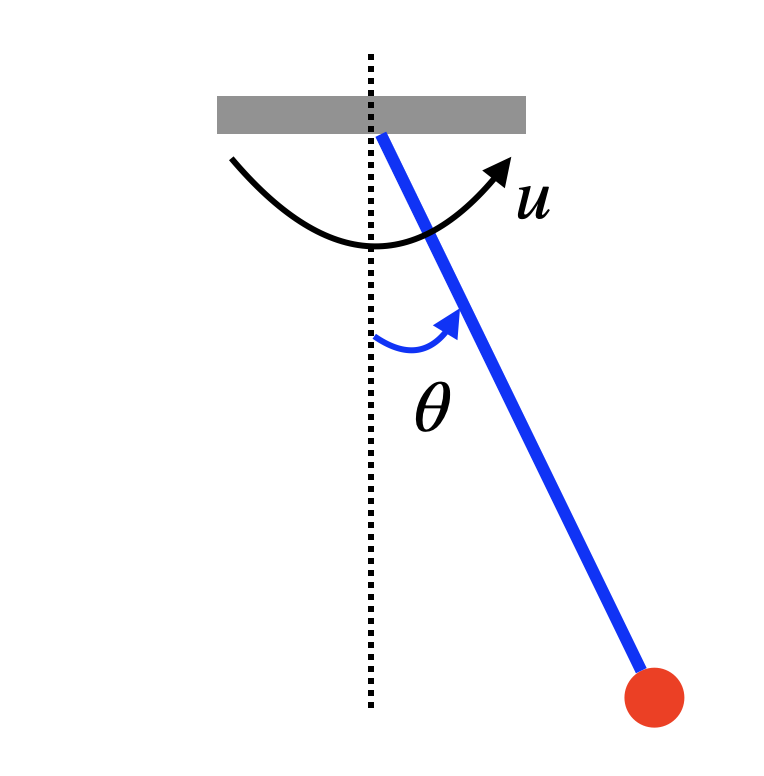
\includegraphics[width=0.4\linewidth]{images/pendulum-drawing} 

}

\caption{A Simple Pendulum.}\label{fig:pendulum-drawing}
\end{figure}

Let us first shift the dynamics so that ``\(0\)'' is the upright position. This can be done by defining a new variable \(z = x - x_d = [\theta - \pi, \dot{\theta}]^T\), which leads to
\begin{equation}
\dot{z} = \dot{x} = f(x,u) = f(z + x_d,u) = \begin{bmatrix}
z_2 \\
\frac{1}{ml^2} \left( u - b z_2 + mgl \sin z_1  \right)
\end{bmatrix} = f'(z,u).
\label{eq:pendulum-dynamics-z-coordinate}
\end{equation}
We then linearize the nonlinear dynamics \(\dot{z} = f'(z,u)\) at the point \(z^\star = 0, u^\star = 0\):
\begin{align}
\dot{z} & \approx f'(z^\star,u^\star) + \left( \frac{\partial f'}{\partial z} \right)_{z^\star,u^\star} (z - z^\star) + \left( \frac{\partial f'}{\partial u} \right)_{z^\star,u^\star} (u - u^\star) \\
& = \begin{bmatrix}
0 & 1 \\
\frac{g}{l} \cos z_1 & - \frac{b}{ml^2}
\end{bmatrix}_{z^\star, u^\star} z + 
\begin{bmatrix}
0 \\
\frac{1}{ml^2}
\end{bmatrix} u \\
& = \underbrace{\begin{bmatrix}
0 & 1 \\
\frac{g}{l} & - \frac{b}{ml^2}
\end{bmatrix}}_{A_c} z  + 
\underbrace{\begin{bmatrix}
0 \\
\frac{1}{ml^2}
\end{bmatrix}}_{B_c} u.
\end{align}
Finally, we convert the continuous-time dynamics to discrete time with a fixed discretization \(h\)
\[
z_{k+1} = \dot{z}_k \cdot h + z_k = \underbrace{(h \cdot A_c + I )}_{A} z_k + \underbrace{(h \cdot B_c)}_{B} u_k.
\]

We are now ready to implement the LQR controller. In the formulation \eqref{eq:infinite-horizon-lqr-cost}, we choose \(Q = I\), \(R = I\), and solve the gain matrix \(K\) using the Matlab \texttt{dlqr} function.

Fig. \ref{fig:pendulum-stabilization-sim} shows the simulation result for \(m=1,l=1,b=0.1\), \(g = 9.8\), and \(h = 0.01\), with an initial condition \(z^0 = [0.1,0.1]^T\). We can see that the LQR controller successfully stabilizes the pendulum at \(z^\star\), the upright position.

You can play with the Matlab code \href{https://github.com/ComputationalRobotics/OptimalControlEstimation-Examples/blob/main/pendulum_stabilization_lqr.m}{here}.

\begin{figure}

{\centering 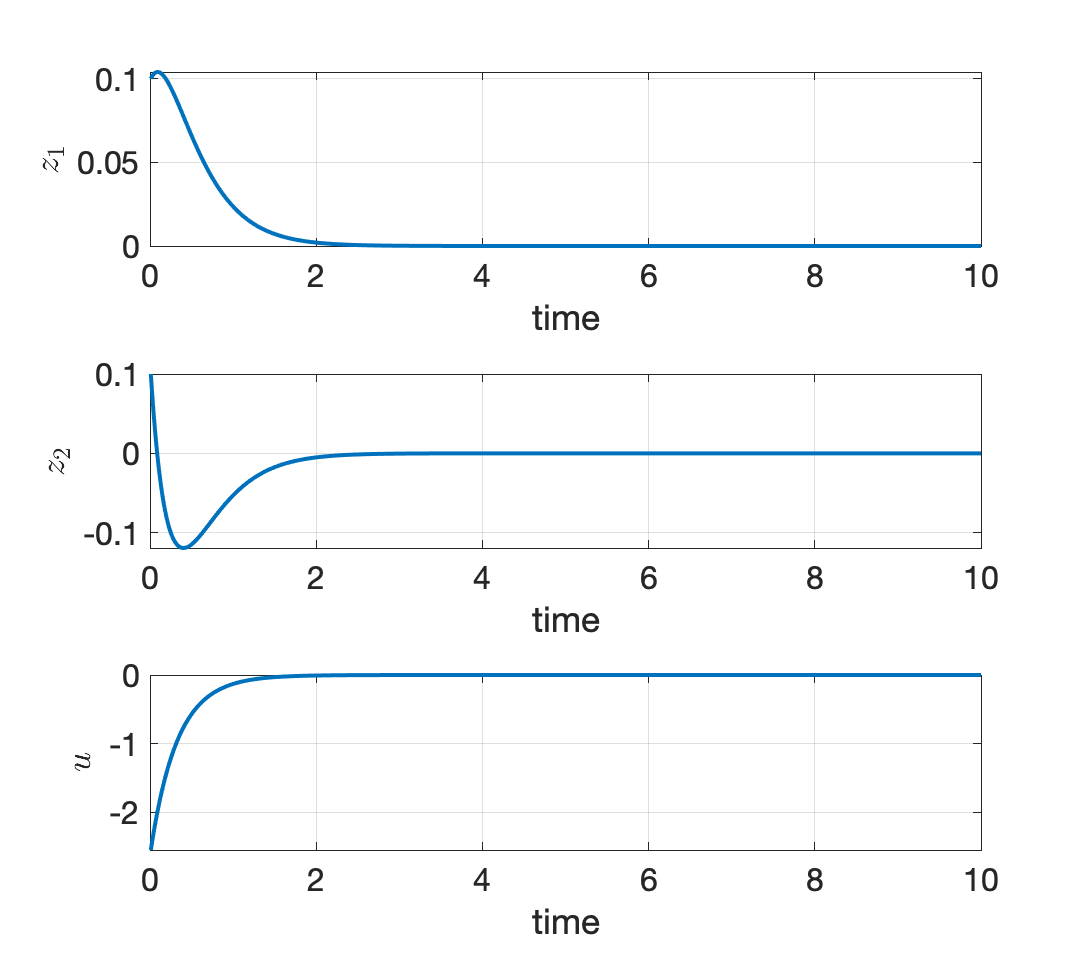
\includegraphics[width=0.6\linewidth]{images/pendulum-stabilization-lqr} 

}

\caption{LQR stabilization of a simple pendulum.}\label{fig:pendulum-stabilization-sim}
\end{figure}

\end{example}

\hypertarget{lqr-with-constraints}{%
\subsection{LQR with Constraints}\label{lqr-with-constraints}}

Let's explore LQR with constraints in Exercise \ref{exr:lqrconstraints}

\hypertarget{mdp-exact-dp}{%
\section{Markov Decision Process}\label{mdp-exact-dp}}

In Section \ref{lqr}, we see that linear dynamics and quadratic costs leads to exact dynamic programming. We now introduce another setup where the number of states and controls is finite (as opposed to the LQR case where \(x_k\) and \(u_k\) live in continuous spaces). We will see that we can execute DP exactly in this setup as well.

Optimal control in the case of finite states and controls is typically introduced in the framework of a \emph{Markov Decision Process} (MDP, which is common in Reinforcement Learning).
There are many variations of a MDP, and here we only focus on the discounted infinite-horizon MDP. For a more complete treatment of MDPs, I suggest checking out \href{https://shamulent.github.io/CS_Stat184_Fall23.html}{this course at Harvard}.

Formally, a discounted infinite-horizon MDP \(\mathcal{M} = (\mathbb{X},\mathbb{U},P,g,\gamma,\sigma)\) is specified by

\begin{itemize}
\item
  a state space \(\mathbb{X}\) that is finite with size \(|\mathbb{X}|\)
\item
  a control space \(\mathbb{U}\) that is finite with size \(|\mathbb{U}|\)
\item
  a transition function \(P: \mathbb{X} \times \mathbb{U} \rightarrow \Delta(\mathbb{X})\), where \(\Delta(\mathbb{X})\) is the space of probability distributions over \(\mathbb{X}\); specifically, \(P(x' \mid x, u)\) is the probability of transitioning into state \(x'\) from state \(x\) using control \(u\). If the system is deterministic, then \(P(x' \mid x, u)\) is nonzero only for a single next state \(x'\)
\item
  a cost function \(g: \mathbb{X} \times \mathbb{U} \rightarrow [0,1]\); \(g(x,u)\) is the cost of taking the control \(u\) at state \(x\)
\item
  a discount factor \(\gamma \in [0,1)\)
\item
  an initial state distribution \(\sigma \in \Delta(\mathbb{X})\) that specifies how the initial state \(x_0\) is generated; in many cases we will assume \(x_0\) is fixed and \(\sigma\) is a distribution supported only on \(x_0\).
\end{itemize}

In an MDP, the system starts at some state \(x_0 \sim \sigma\). At each step \(k = 0,1,2,\dots\), the system decides a control \(u_k \in \mathbb{U}\) and incurs a cost \(g(s_k,u_k)\). The control \(u_k\) brings the system into a new state \(x_{k+1} \sim P(\cdot \mid x_k, u_k)\), at which the controller decides a new control \(u_{k+1}\). This process continues forever.

\textbf{Controller (policy)}. In general, a time-varying controller \(\pi = (\pi_0,\dots,\pi_k,\dots)\) is a mapping from all previous states and controls to a distribution over current controls. The mapping \(\pi_k\) at timestep \(k\) is
\[
\pi_k: (x_0,u_0,x_1,u_1,\dots,x_k) \mapsto u_k \sim q_k \in \Delta(\mathbb{U}).
\]
Note that \(u_k\) can be randomized and it is drawn from a distribution \(q_k\) supported on the set of controls \(\mathbb{U}\).
A \emph{stationary} controller (policy) \(\pi: \mathbb{X} \rightarrow \Delta(\mathbb{U})\) specifies a decison-making strategy that is purely based on the current state \(x_k\). A \emph{deterministic} and stationary controller \(\pi: \mathbb{X} \rightarrow \mathbb{U}\) excutes a deterministic control \(u_k\) at each step.

\textbf{Cost-to-go and \(Q\)-value}. Given a controller \(\pi\) and an initial state \(x_0\), we associate with it the following discounted infinite-horizon cost
\begin{equation}
J_\pi(x_0) = \mathbb{E} \left\{ \sum_{k=0}^{\infty} \gamma^k g(x_k, u_k^{\pi}) \right\},
\label{eq:mdp-cost-policy}
\end{equation}
where the expectation is taken over the randomness of the transition \(P\) and the controller \(\pi\). Note that we have used \(u^{\pi}_k\) to denote the control at step \(k\) by following the controller \(\pi\). Similarly, we define the \(Q\)-value function as
\begin{equation}
Q_\pi(x_0,u_0) = \mathbb{E} \left\{  g(x_0,u_0) + \sum_{k=1}^{\infty} \gamma^k g(x_k,u_k^{\pi}) \right\}.
\label{eq:mdp-Q-value}
\end{equation}
The difference between \(Q_\pi(x_0,u_0)\) and \(J_\pi(x_0)\) is that at step zero, \(J_\pi(x_0)\) follows the controller \(\pi\) while \(Q_\pi(x_0,u_0)\) assumes the control \(u_0\) is given. By the assumption that \(g(x_k,u_k) \in [0,1]\), we have
\[
0 \leq J_\pi(x_0), Q_\pi(x_0,u_0) \leq \sum_{k=0}^{\infty} \gamma^k = \frac{1}{1-\gamma}, \quad \forall \pi.
\]

Our goal is to find the best controller that minimizes the cost function
\begin{equation}
\pi^\star \in \arg\min_{\pi \in \Pi} J_\pi(x_0)
\label{eq:mdp-objective}
\end{equation}
for a given initial state \(x_0\), where \(\Pi\) is the space of all non-stationary and randomized controllers.

A remarkable property of MDPs is that there exists an optimal controller that is stationary and deterministic.

\begin{theorem}[Deterministic and Stationary Optimal Policy]
\protect\hypertarget{thm:optimalmdppolicystationary}{}\label{thm:optimalmdppolicystationary}Let \(\Pi\) be the space of all non-stationary and randomized policies. Define
\[
J^\star_\pi(x) = \min_{\pi \in \Pi} J_\pi(x), \quad Q^\star_\pi(x,u) = \min_{\pi \in \Pi } Q_\pi(x,u).
\]
There exists a deterministic and stationary policy \(\pi^\star\) such that for all \(x \in \mathbb{X}\) and \(u \in \mathbb{U}\),
\[
J_{\pi^\star}(x) = J^\star(x), \quad Q_{\pi^\star}(x,u) = Q^\star(x,u).
\]
We call such a policy \(\pi\) an optimal policy.
\end{theorem}

\begin{proof}
See Theorem 1.7 in \citep{agarwal22book-reinforcement}.
\end{proof}

This Theorem shows that we can restrict ourselves to stationary and deterministic policies without losing performance.

In the next, we show how to characterize the optimal policy and value function.

\hypertarget{bellman-optimality-equations}{%
\subsection{Bellman Optimality Equations}\label{bellman-optimality-equations}}

We now restrict ourselves to stationary policies. We first introduce the Bellman Consistency Equations for stationary policies.

\begin{lemma}[Bellman Consistency Equations]
\protect\hypertarget{lem:mdpbellmanconsistency}{}\label{lem:mdpbellmanconsistency}Let \(\pi\) be a stationary policy. Then \(J_\pi\) and \(Q_\pi\) satisfy the following Bellman consistency equations
\begin{align}
J_\pi(x) &= \mathbb{E}_{u \sim \pi(\cdot \mid x)} Q_\pi(x,u), \label{eq:bellman-consistency-1} \\
Q_\pi(x,u) &=g(x,u) + \gamma \mathbb{E}_{x' \sim P(\cdot \mid x,u)} J_\pi(x'). \label{eq:bellman-consistency-2}
\end{align}
\end{lemma}

\begin{proof}
By the definition of the cost-to-go function in \eqref{eq:mdp-cost-policy}, we have
\[
J_\pi(x_0) = \mathbb{E}\left\{ \sum_{k=0}^{\infty} \gamma^k g(x_k, \pi(x_k))  \right\} = \mathbb{E}_{u_0 \sim \pi(\cdot \mid x_0)} \underbrace{\mathbb{E} \left\{ g(x_0,u_0) + \sum_{k=1}^{\infty} \gamma^k g(x_k,\pi(x_k)) \right\}}_{Q_\pi(x_0,u_0)}.
\]
The above equation holds for any \(x_0\), proving \eqref{eq:bellman-consistency-1}.

To show \eqref{eq:bellman-consistency-2}, we recall the definition of the \(Q\)-value function \eqref{eq:mdp-Q-value}
\begin{align}
Q_\pi(x_0,u_0) & = \mathbb{E} \left\{ g(x_0,u_0) + \sum_{k=1}^{\infty} \gamma^k g(x_k,\pi(x_k)) \right\}  \\
&=  g(x_0,u_0) + \gamma \mathbb{E} \left\{ \sum_{k=1}^{\infty} \gamma^{k-1} g(x_k,\pi(x_k)) \right\} \label{eq:bellman-constency-proof-1}
\end{align}
Now observe that the expectation of the second term in \eqref{eq:bellman-constency-proof-1} is taken over both the randomness of \(x_1\) and the randomness of the policy after \(x_1\) is reached. Therefore,
\[
\mathbb{E} \left\{ \sum_{k=1}^{\infty} \gamma^{k-1} g(x_k,\pi(x_k)) \right\} = \mathbb{E}_{x_1 \sim P(\cdot \mid x_0,u_0)} \underbrace{\left\{ \mathbb{E} \left\{ \sum_{k=1}^{\infty} \gamma^{k-1} g(x_1,\pi(x_1)) \right\} \right\}}_{J_\pi(x_1)}.
\]
Plugging the above equation back to \eqref{eq:bellman-constency-proof-1}, we obtain the desired result in \eqref{eq:bellman-consistency-2}.
\end{proof}

\textbf{Matrix Representation}. It is useful to think of \(P,g,J_\pi,Q_\pi\) as matrices. In particular, the transition function \(P\) can be considered as a matrix of dimension \(|\mathbb{X}||\mathbb{U}| \times \mathbb{X}\), where
\[
P_{(x,u),x'} = P(x' \mid x,u)
\]
is the entry of \(P\) at the row \((x,u)\) (there are \(|\mathbb{X}||\mathbb{U}|\) such rows) and column \(x'\) (there are \(|\mathbb{X}|\) such columns). The running cost \(g\) is vector of \(|\mathbb{X}||\mathbb{U}|\) entries. The cost-to-go \(J_\pi(x)\) is a vector of \(|\mathbb{X}|\) entries. The \(Q\)-value function \(Q_\pi(x,u)\) is a vector of \(|\mathbb{X}||\mathbb{U}|\) entries. We also introduce \(P^{\pi}\) with dimension \(|\mathbb{X}||\mathbb{U}| \times |\mathbb{X}||\mathbb{U}|\) as the transition matrix induced by a stationary policy \(\pi\). In particular,
\[
P^\pi_{(x,u),(x',u')} = P(x' \mid x,u) \pi(u'\mid x').
\]
In words, \(P^\pi_{(x,u),(x',u')}\) is the probability that \((x',u')\) follows \((x,u)\).

With the matrix representation, we can compactly write the Bellman consistency equation \eqref{eq:bellman-consistency-2} as
\begin{equation}
Q_\pi = g + \gamma P J_\pi.
\label{eq:bellman-consistency-2-matrix}
\end{equation}
We can also combine \eqref{eq:bellman-consistency-1} and \eqref{eq:bellman-consistency-2} together and write
\[
Q_\pi(x,u) = g(x,u) + \gamma \mathbb{E}_{x' \sim P(\cdot \mid x,u)} \left\{ \mathbb{E}_{u' \sim \pi(\cdot \mid x')} Q_\pi(x',u') \right\} = g(x,u) + \gamma \mathbb{E}_{(x',u') \sim P^\pi(\cdot \mid (x,u))} Q_\pi(x',u'),
\]
which, using matrix representation, becomes
\begin{equation}
Q_\pi = g + \gamma P^\pi Q_\pi.
\label{eq:bellman-consistency-2-matrix-2}
\end{equation}
Equation \eqref{eq:bellman-consistency-2-matrix-2} immediately yields
\begin{equation}
Q_\pi = (I - \gamma P^\pi)^{-1} g,
\label{eq:bellman-consistency-Qpi-linearsystem}
\end{equation}
that is, the \(Q\)-value function associated with a stationary policy \(\pi\) can be simply computed from solving a linear system as in \eqref{eq:bellman-consistency-Qpi-linearsystem}.\footnote{One can show that the matrix \(I - \gamma P^\pi\) is indeed invertible, see Corollary 1.5 in \citep{agarwal22book-reinforcement}.}

Lemma \ref{lem:mdpbellmanconsistency}, together with the equivalent matrix equations \eqref{eq:bellman-consistency-2-matrix} and \eqref{eq:bellman-consistency-2-matrix-2}, provide the conditions that \(J_\pi\) and \(Q_\pi\), induced by any stationary policy \(\pi\), need to satisfy. In the next, we describe the conditions that characterize the optimal policy.

\begin{theorem}[Bellman Optimality Equations]
\protect\hypertarget{thm:mdpbellmanoptimality}{}\label{thm:mdpbellmanoptimality}A vector \(Q \in \mathbb{R}^{|\mathbb{X}||\mathbb{U}|}\) is said to satisfy the Bellman optimality equation if
\begin{equation}
Q(x,u) = g(x,u) + \gamma \mathbb{E}_{x' \sim P(\cdot \mid x,u)} \left\{ \min_{u' \in \mathbb{U}} Q(x',u') \right\}, \quad \forall (x,u) \in \mathbb{X} \times \mathbb{U}.
\label{eq:bellman-optimality-equation}
\end{equation}

A vector \(Q^\star\) is the optimal \(Q\)-value function if and only if it satisfies \eqref{eq:bellman-optimality-equation}. Moreover, the deterministic policy defined by
\[
\pi^\star(x) \in \arg\min_{u \in \mathbb{U}} Q^\star(x,u)
\]
with ties broken arbitrarily is an optimal policy.
\end{theorem}

\begin{proof}
See Theorem 1.8 in \citep{agarwal22book-reinforcement}.
\end{proof}

We now make a few definitions to interpret Theorem \ref{thm:mdpbellmanoptimality}. For any vector \(Q \in \mathbb{R}^{|\mathbb{X}||\mathbb{U}|}\), define the greedy policy as
\begin{equation}
\pi_{Q}(x) \in \arg\min_{u \in \mathbb{U}} Q(x,u)
\label{eq:def-pi-Q}
\end{equation}
with ties broken arbitrarily. With this notation, by Theorem \ref{thm:mdpbellmanoptimality}, the optimal policy is
\[
\pi^\star = \pi_{Q^\star},
\]
where \(Q^\star\) is the optimal \(Q\)-value function. Similarly, let us define
\[
J_Q(x) = \min_{u \in \mathbb{U}} Q(x,u).
\]
Note that \(J_Q\) has dimension \(|\mathbb{X}|\). With these notations, the \emph{Bellman optimality operator} is defined as
\begin{equation}
\mathcal{T}Q = g + \gamma P J_Q,
\label{eq:bellman-optimality-operator}
\end{equation}
which is nothing but a matrix representation of the right-hand side of \eqref{eq:bellman-optimality-equation}. This allows us to concisely write the Bellman optimality equation \eqref{eq:bellman-optimality-equation} as
\begin{equation}
Q = \mathcal{T}Q.
\label{eq:mdp-fixed-point}
\end{equation}
Therefore, an equivalent way to interpret Theorem \ref{thm:mdpbellmanoptimality} is that \(Q = Q^\star\) if and only if \(Q\) is a fixed point to the Bellman optimality operator \(\mathcal{T}\).

\hypertarget{value-iteration}{%
\subsection{Value Iteration}\label{value-iteration}}

Intepreting the optimal \(Q\)-value function as the fixed point to the Bellman optimality operator \eqref{eq:mdp-fixed-point} leads us to a natural algorithm for solving the optimal control problem.

We start with \(Q^{(0)}\) being an all-zero vector and then at iteration \(t\), we perform
\[
Q^{(t+1)} \leftarrow \mathcal{T} Q^{(t)},
\]
with \(\mathcal{T}\) defined in \eqref{eq:bellman-optimality-operator}. Let us observe the simplicity of this algorithm: at each iteration, one only needs to perform \(\min_{u \in \mathbb{U}} Q^{(t)}(x,u)\), which is very efficient when \(|\mathbb{U}|\) is not too large.

The next theorem states this simple algorithm converges to the optimal value function.

\begin{theorem}[Value Iteration]
\protect\hypertarget{thm:valueiteration}{}\label{thm:valueiteration}Set \(Q^{(0)} = 0\). For \(t=0,\dots\), perform
\[
Q^{(t+1)} \leftarrow \mathcal{T} Q^{(t)}.
\]
Let \(\pi^{(k)} = \pi_{Q^{(k)}}\) (see the definition in \eqref{eq:def-pi-Q}). For \(t \geq \frac{\log \frac{2}{(1-\gamma)^2 \epsilon}}{1-\gamma}\), we have
\[
J^{\pi^{(t)}} \leq J^\star + \epsilon \mathbb{1},
\]
where \(\mathbb{1}\) is the all-ones vector.
\end{theorem}

Essentially, the value function obtained from value iteration converges to the optimal cost-to-go.

Let us use an example to appreciate this algorithm.

\begin{example}[Shortest Path in Grid World]
\protect\hypertarget{exm:gridworld}{}\label{exm:gridworld}

Consider the following \(10 \times 10\) grid world, where the top-right cell is the goal location, and the dark blue colored cells are obstacles.

\begin{figure}

{\centering 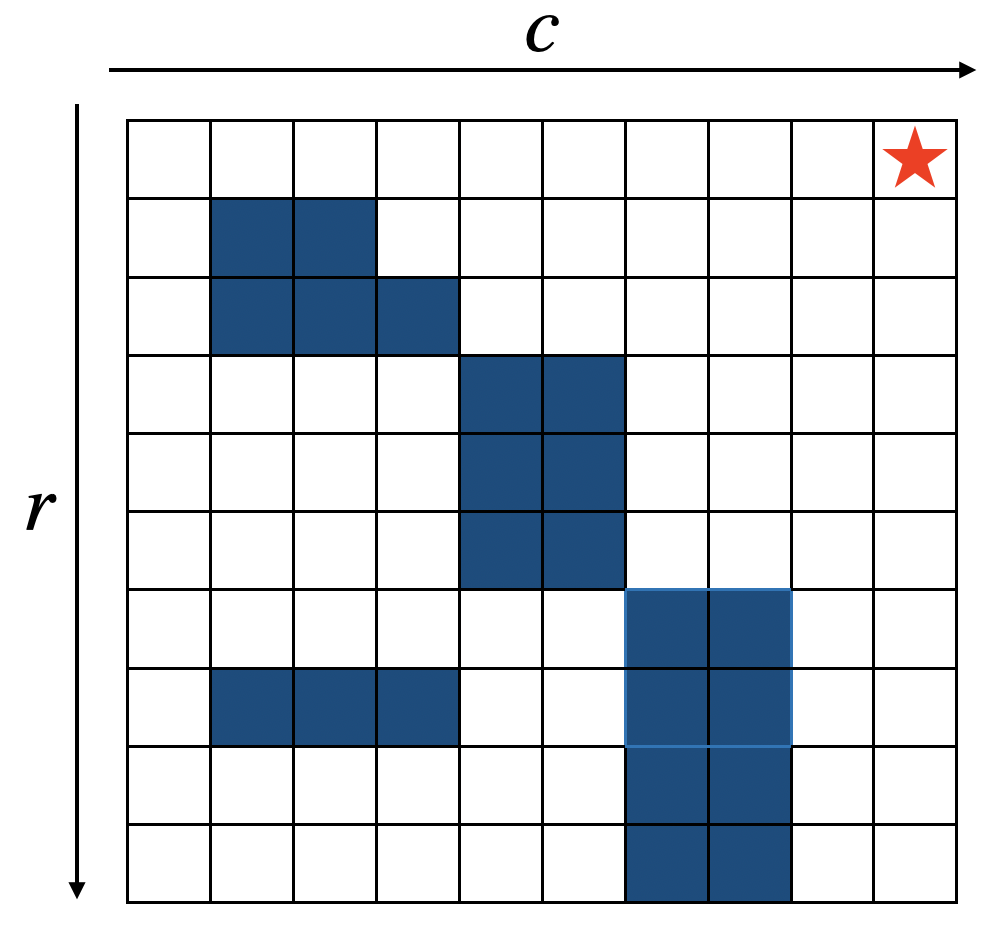
\includegraphics[width=0.5\linewidth]{images/grid-world-obstacle} 

}

\caption{Grid World with Obstacles.}\label{fig:grid-world}
\end{figure}

We want to find the shortest path from a given cell to the target cell, while not hitting obstacles.

To do so, we set the state space of the system as
\[
\mathbb{X} = \left\{ \begin{bmatrix} r \\ c \end{bmatrix} \middle\vert r,c \in \{ 1,\dots,10 \} \right\}
\]
where \(r\) is the row index (from top to bottom) and \(c\) is the column index (from left to right). The control space is moving left, right, up, down, or do nothing:
\[
\mathbb{U} = \left\{ 
    \begin{bmatrix} 1 \\ 0 \end{bmatrix},
    \begin{bmatrix} -1 \\ 0 \end{bmatrix},
    \begin{bmatrix} 0 \\ 1 \end{bmatrix},
    \begin{bmatrix} 0 \\ -1 \end{bmatrix},
    \begin{bmatrix} 0 \\ 0 \end{bmatrix}
    \right\}.
\]
The system dynamics is deterministic
\[
x' = \begin{cases}
x + u & \text{if } x + u \text{ is inside the grid} \\
x & \text{otherwise}
\end{cases}.
\]
We then design the following running cost function \(g\)
\[
g(x,u) = \begin{cases}
0 & \text{if } x = [1,10]^T \text{ is the target} \\
20 & \text{if } x \text{ is an obstacle} \\
1 & \text{otherwise}
\end{cases}.
\]
Note that \(g(x,u)\) defined above does not even satisfy \(g \in [0,1]\). We then use value iteration to solve the optimal control problem with \(\gamma = 1\)
\[
J(x_0) = \min_{\pi} \sum_{k=0}^{\infty} g(x_k,\pi(x_k)).
\]

The \href{https://github.com/ComputationalRobotics/OptimalControlEstimation-Examples/blob/main/grid_world_value_iteration.m}{Matlab script} of value iteration converges in \(27\) iterations, and we obtain the optimal cost-to-go in Fig. \ref{fig:grid-world-solution}.

Starting from the cell \([8,5]^T\), the red line in Fig. \ref{fig:grid-world-solution} plots the optimal trajectory that clearly avoids the obstacles.

Feel free to play with the size of the grid and the number of obstacles.

\begin{figure}

{\centering 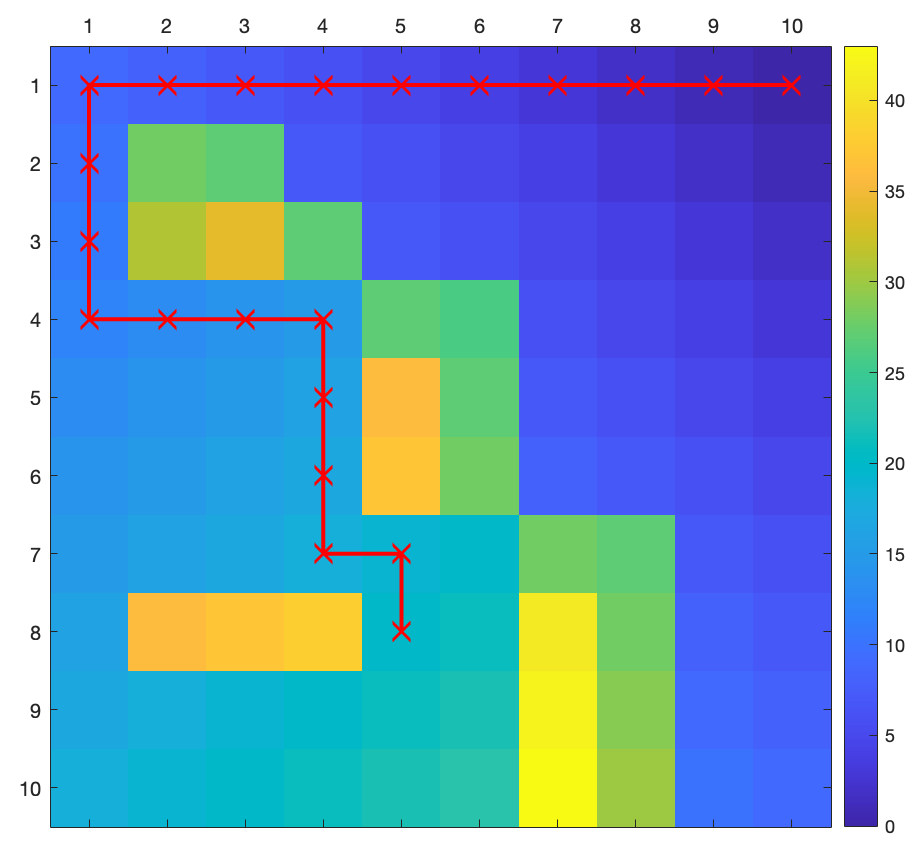
\includegraphics[width=0.5\linewidth]{images/grid-world-solution} 

}

\caption{Optimal cost-to-go and an optimal trajectory.}\label{fig:grid-world-solution}
\end{figure}

\end{example}

Example \ref{exm:gridworld} shows the simplicity and power of value iteration. However, the states and controls in the grid world are naturally discrete and finite. Is it possible to apply value iteration to optimal control problems where the states and controls live in continuous spaces?

\hypertarget{value-iteration-with-barycentric-interpolation}{%
\subsection{Value Iteration with Barycentric Interpolation}\label{value-iteration-with-barycentric-interpolation}}

Let us consider the discrete-time dynamics
\[
x_{k+1} = f(x_k, u_k)
\]
where both \(x_k\) and \(u_k\) live in a continuous space, say \(\mathbb{R}^{n}\) and \(\mathbb{R}^m\), respectively.

A natural idea to apply value iteration is to discretize the state space and control space. For example, suppose \(x \in \mathbb{R}^2\) and we have discretized \(\mathbb{R}^2\) using \(N\) points
\[
\mathcal{S} = \{s_1,\dots,s_N\}
\]
that lie on a 2D grid, as shown in Fig. \ref{fig:barycentric-interpolation}. Assume \(x_k \in \mathcal{S}\) lies on the mesh grid, the next state \(x_{k+1} = f(x_k,u_k)\) will, however, most likely not lie exactly on one of the grid points.

\begin{figure}

{\centering 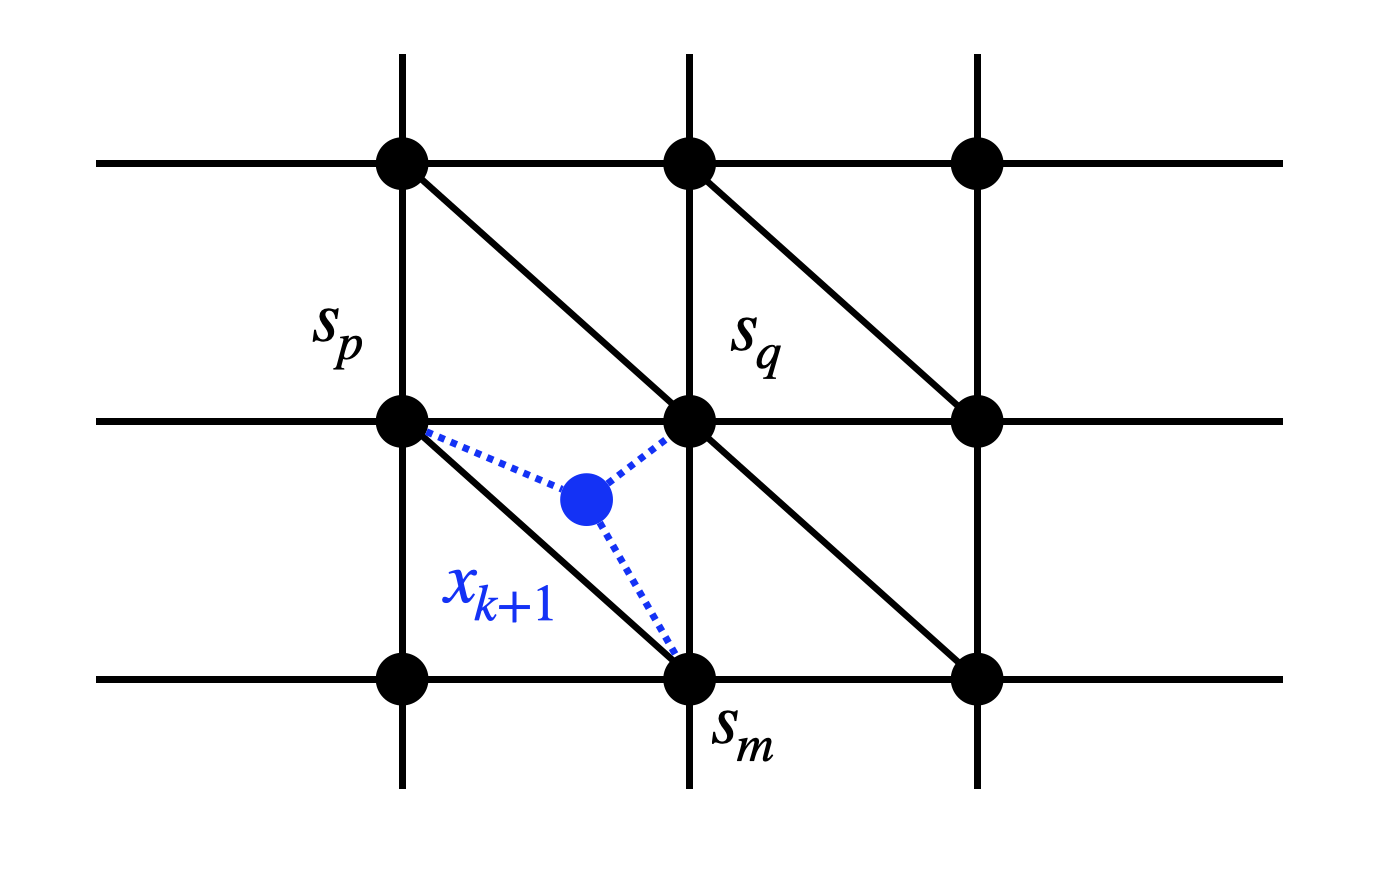
\includegraphics[width=0.5\linewidth]{images/barycentric-coordinate} 

}

\caption{Barycentric Interpolation.}\label{fig:barycentric-interpolation}
\end{figure}

Nevertheless, \(x_{k+1}\) will lie inside a triangle with vertices \(s_p, s_q, s_m\). We will now try to write \(x_{k+1}\) using the vertices, that is, to find three numbers \(\lambda_p, \lambda_q, \lambda_m\) such that
\[
\lambda_p, \lambda_q, \lambda_m \geq 0, \quad \lambda_p + \lambda_q + \lambda_m = 1, \quad x_{k+1} = \lambda_p s_p + \lambda_q s_q + \lambda_m s_m.
\]
\(\lambda_p,\lambda_q,\lambda_m\) are called the barycentric coordinates of \(x_{k+1}\) in the triangle formed by \(s_p,s_q,s_m\). With the barycentric coordinates, we will assign the transition matrix
\[
P(x_{k+1}=s_p \mid x_k,u_k) = \lambda_p, \quad P(x_{k+1}=s_q \mid x_k,u_k) = \lambda_q, \quad P(x_{k+1}=s_m \mid x_k,u_k) = \lambda_m.
\]

Let us apply value iteration with barycentric interpolation to the simple pendulum.

\begin{example}[Value Iteration with Barycentric Interpolation on A Simple Pendulum]
\protect\hypertarget{exm:pendulumvalueiterationbarycentric}{}\label{exm:pendulumvalueiterationbarycentric}Consider the continuous-time pendulum dynamics in \eqref{eq:pendulum-dynamics-z-coordinate} that is already shifted such that \(z=0\) corresponds to the upright position. With time discretization \(h\), we can write the discrete-time dynamics as
\[
z_{k+1} = \dot{z}_k \cdot h + z_k = f'(z_k,u_k) \cdot h + z_k.
\]
We are interested in solving the optimal control problem
\[
J(z_0) = \min_{u_k} \left\{ \sum_{k=0}^{\infty} \gamma^k g(x_k,u_k) \right\},
\]
where the running cost is simply
\[
g(x_k,u_k) = x_k^T x_k + u_k^2.
\]

We will use the parameters \(m=1,g=9.8,l=1,b=0.1\), and assume the control is bounded in \([-4.9,4.9]\).

We want to compute the optimal cost-to-go in the range \(z_1 \in [-\pi,\pi]\) and \(z_2 \in [-\pi,\pi]\). We discretize both \(z_1\) and \(z_2\) using \(N\) points, leading to \(N^2\) points in the state space. We also discretize \(u\) using \(N\) points.

Applying value iteration with \(\gamma=0.9\) and \(N=50\), we obtain the optimal cost-to-go in Fig. \ref{fig:pendulum-VI-J-9}. The value iteration converges in \(277\) iterations.

\begin{figure}

{\centering 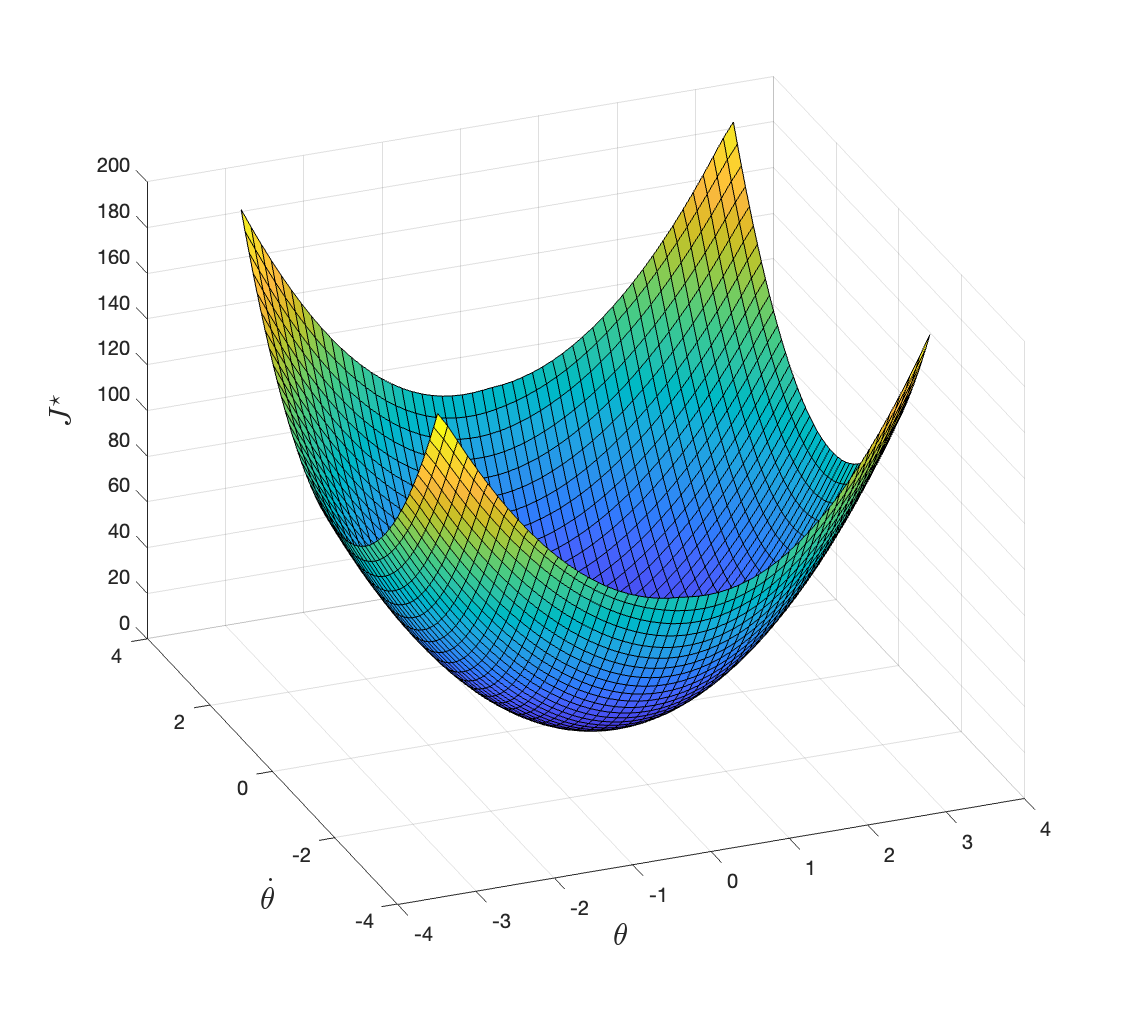
\includegraphics[width=0.5\linewidth]{images/pendulum-VI-J-0.9-1} 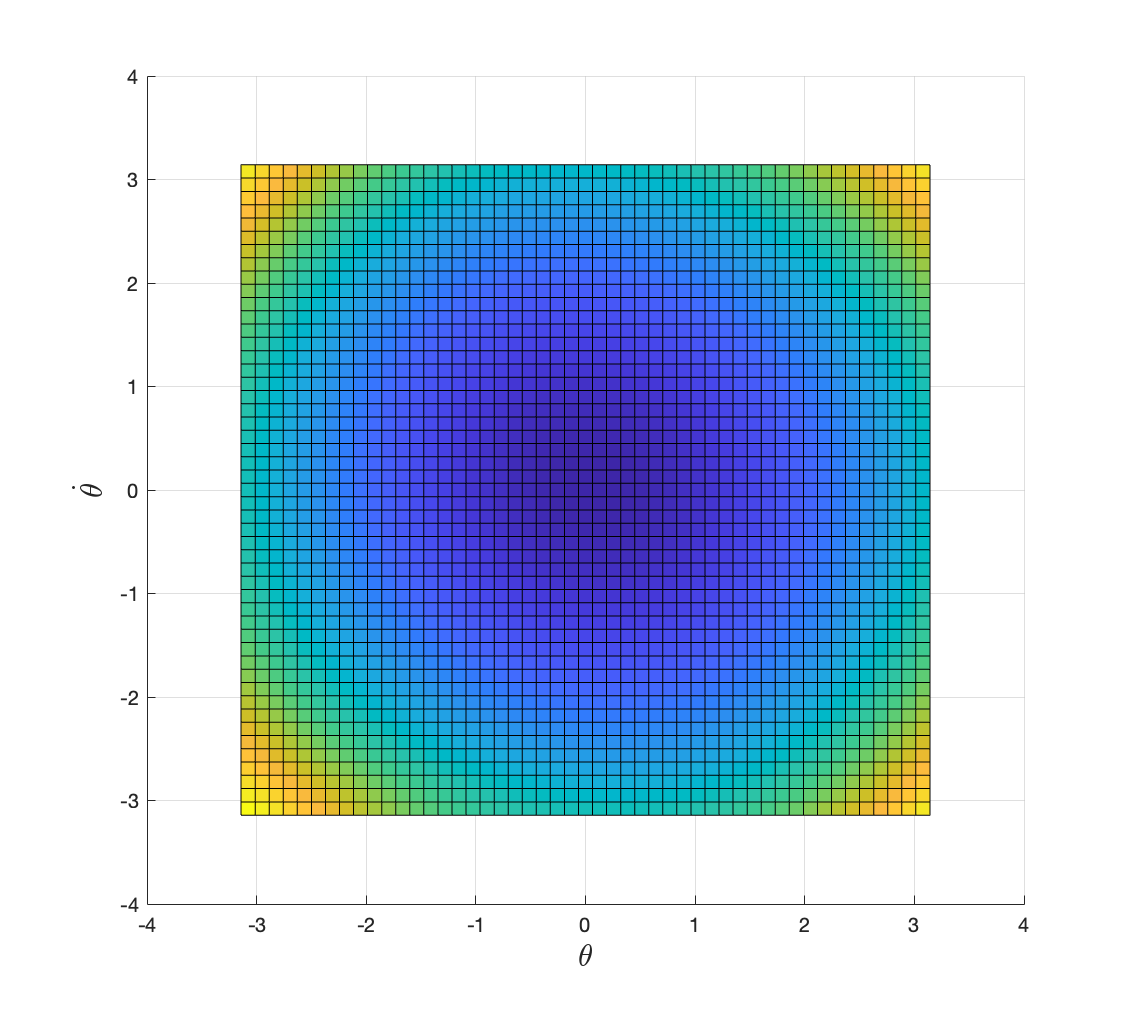
\includegraphics[width=0.5\linewidth]{images/pendulum-VI-J-0.9-2} 

}

\caption{Optimal cost-to-go with discount factor 0.9.}\label{fig:pendulum-VI-J-9}
\end{figure}

Applying value iteration with \(\gamma=0.99\) and \(N=50\), we obtain the optimal cost-to-go in Fig. \ref{fig:pendulum-VI-J-99}. The value iteration converges in \(2910\) iterations.

\begin{figure}

{\centering 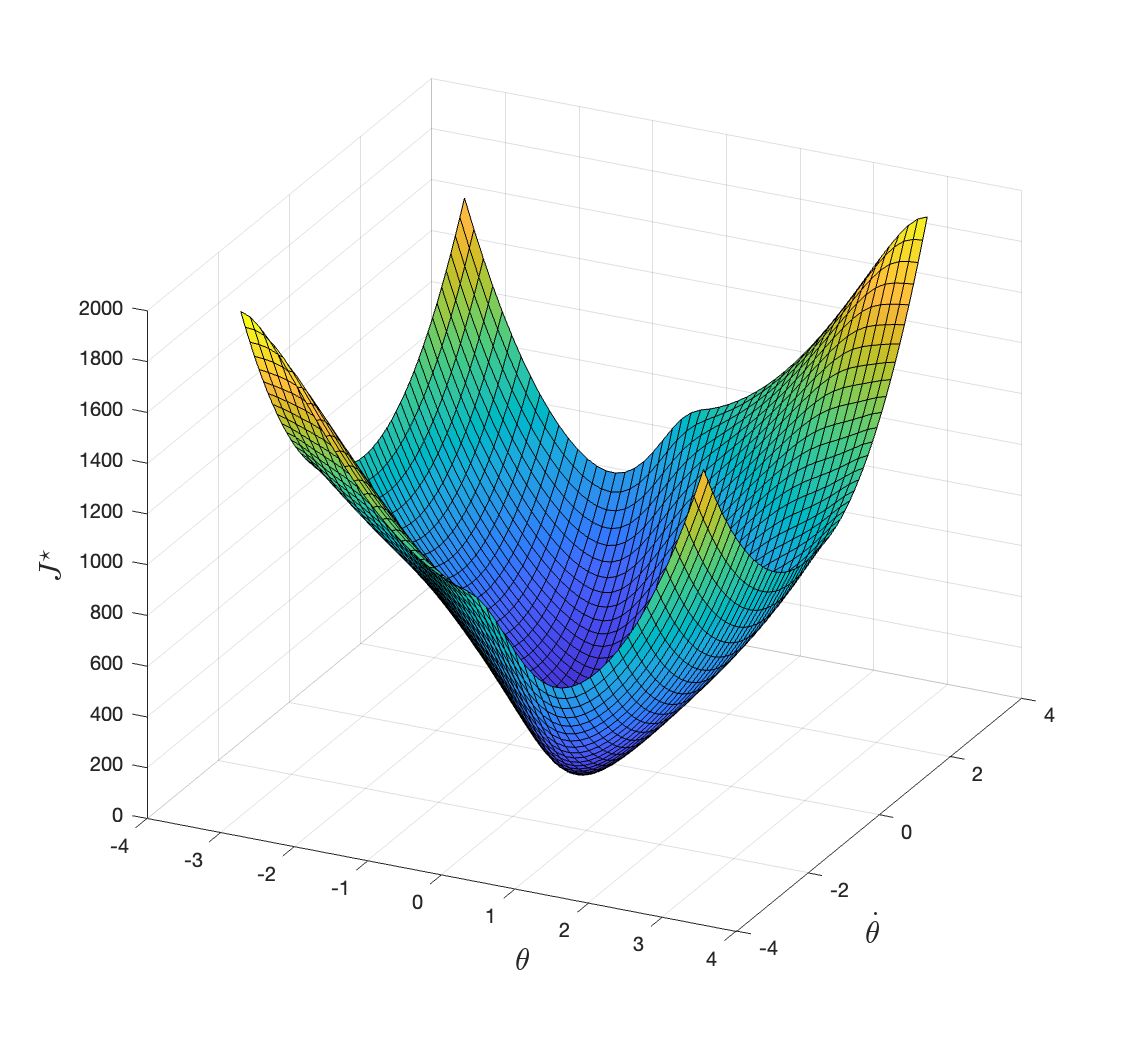
\includegraphics[width=0.5\linewidth]{images/pendulum-VI-J-0.99-1} 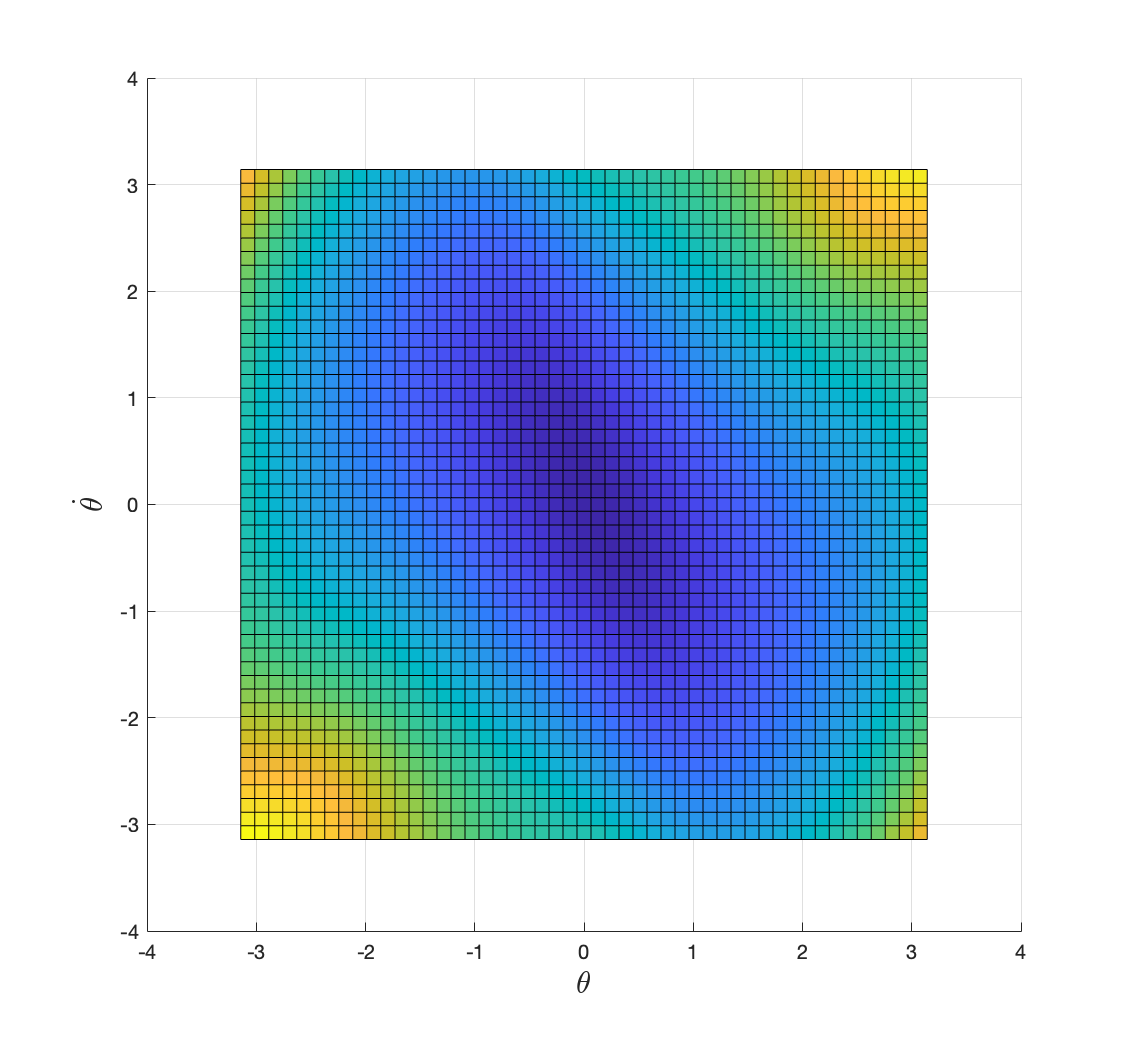
\includegraphics[width=0.5\linewidth]{images/pendulum-VI-J-0.99-2} 

}

\caption{Optimal cost-to-go with discount factor 0.99.}\label{fig:pendulum-VI-J-99}
\end{figure}

Applying value iteration with \(\gamma=0.999\) and \(N=50\), we obtain the optimal cost-to-go in Fig. \ref{fig:pendulum-VI-J-999}. The value iteration converges in \(28850\) iterations.

\begin{figure}

{\centering 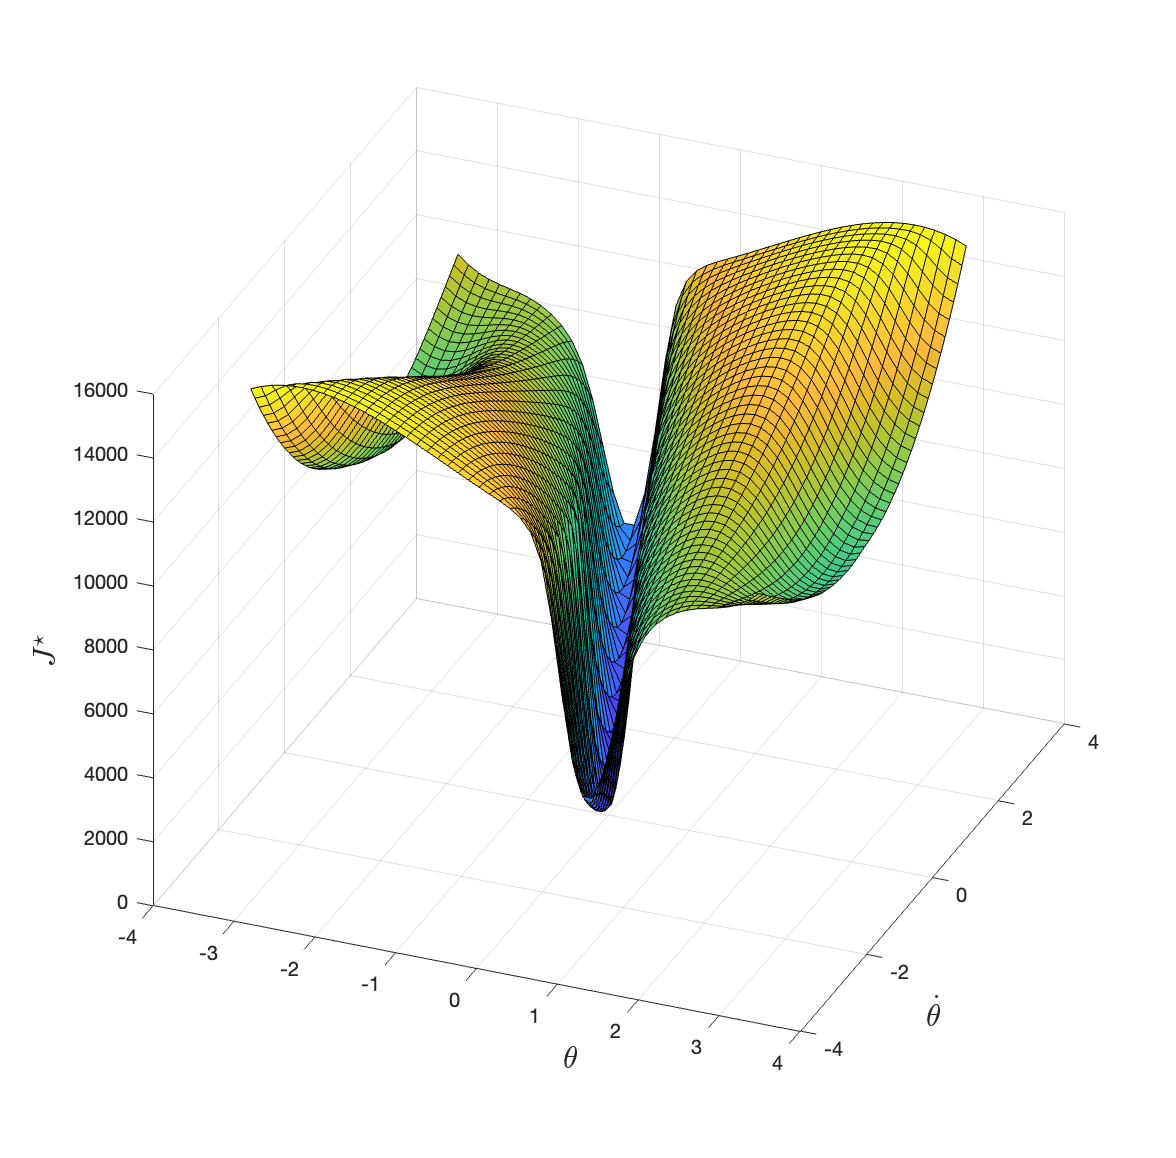
\includegraphics[width=0.5\linewidth]{images/pendulum-VI-J-0.999-1} 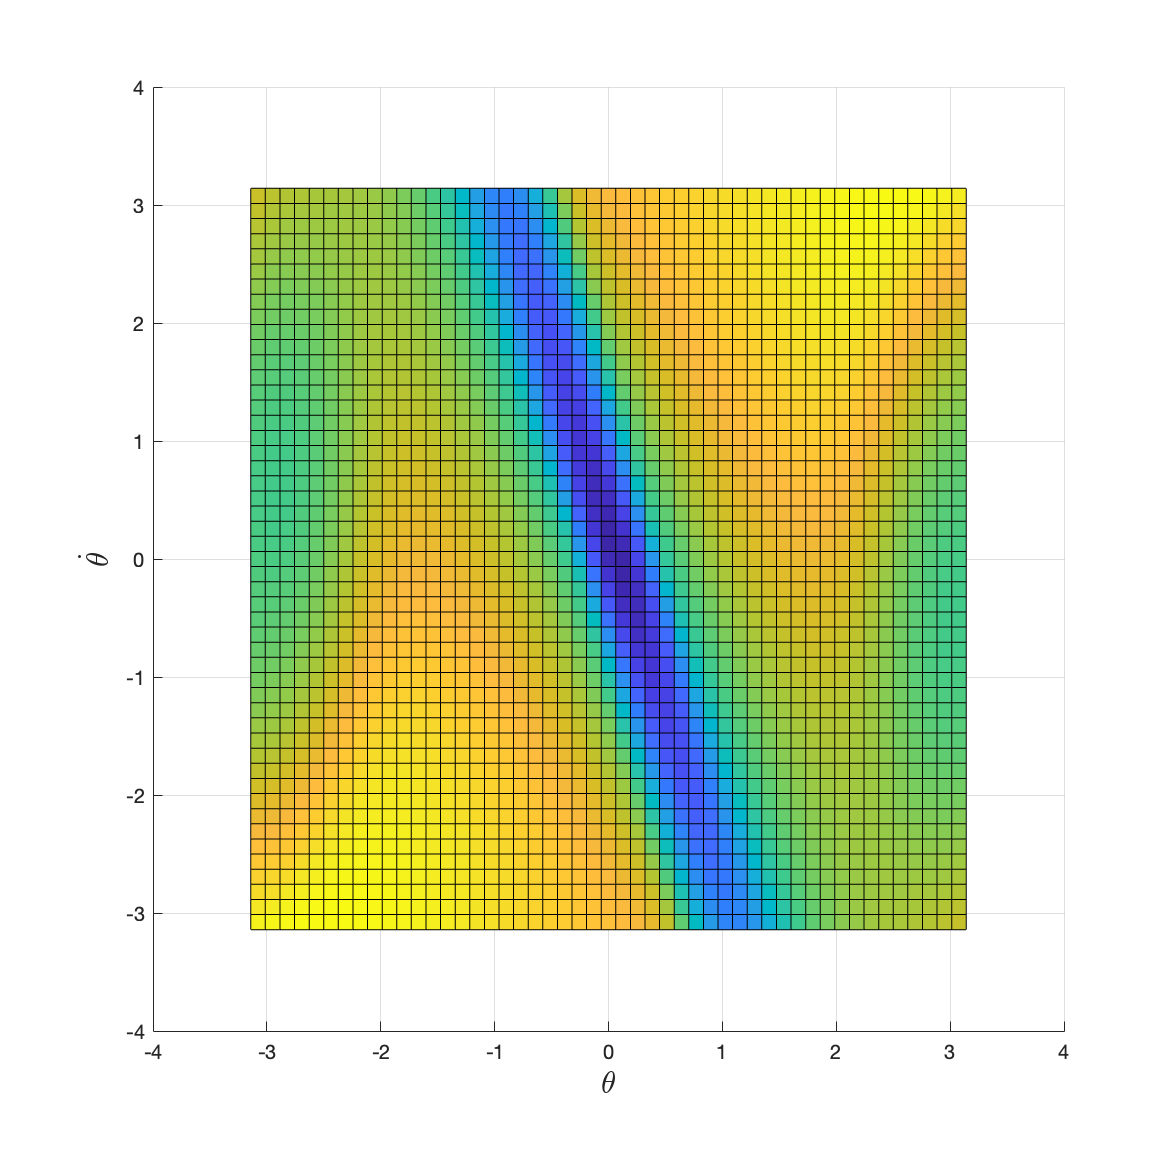
\includegraphics[width=0.5\linewidth]{images/pendulum-VI-J-0.999-2} 

}

\caption{Optimal cost-to-go with discount factor 0.999.}\label{fig:pendulum-VI-J-999}
\end{figure}

You can find the Matlab code \href{https://github.com/ComputationalRobotics/OptimalControlEstimation-Examples/blob/main/pendulum_value_iteration_barycentric.m}{here}.
\end{example}

\hypertarget{approximatedp}{%
\chapter{Approximate Optimal Control}\label{approximatedp}}

\emph{Thanks to \href{https://jrli.org/}{Jiarui Li} for contributing to this Chapter.}

In Chapter \ref{exactdp}, we have studied two cases where dynamic programming (DP) can be executed exactly. Both cases are interesting yet limiting.

In the linear quadratic regulator (LQR) case, the optimal controller is a linear controller and it does not require discretization of the state and control space. However, LQR only handles systems with linear dynamics.

In the Markov Decision Process (MDP) case, value iteration can obtain the optimal cost-to-go (or the optimal \(Q\)-value function) usually in a finite number of iterations. With barycentric interpolation, value iteration also leads to a practical controller for swinging up the pendulum (see Example \ref{exm:pendulumvalueiterationbarycentric}), at least starting from some initial states. However, value iteration suffers from the \emph{curse of dimensionality}, i.e., the amount of memory and computation needed to compute the optimal cost-to-go grows exponentially with the number of grids used to discretize the state space and control space.

In this Chapter, we will study approximate dynamic programming, which aims to not find the optimal controller (simply because it is too demanding), but only a suboptimal controller that is perhaps good enough. It is worth noting that there exists a large amount of algorithms and literature for approximate DP, most of which are closely related to reinforcement learning, and studying all of them is beyond the scope of this course. In the following we will only go through several algorithmic frameworks that are representative.

\hypertarget{fitted-value-iteration}{%
\section{Fitted Value Iteration}\label{fitted-value-iteration}}

Let us consider the infinite-horizon optimal control problem introduced in Chapter \ref{infinite-horizon}
\[
\min_{\pi} \mathbb{E} \left\{ \sum_{k=0}^\infty g(x_k, \pi(x_k)) \right\}.
\]
Under some technical conditions, we know that the optimal policy is a deterministic and stationary policy and the optimal cost-to-go satisfies the following Bellman Optimality Equation
\begin{equation}
J^\star(x) = \min_{u \in \mathbb{U}} \mathbb{E}_w \left\{ g(x,u) + J^\star(f(x,u,w)) \right\}, \quad \forall x \in \mathbb{X}.
\label{eq:bellmanoptimality-fvi}
\end{equation}
From the plots in Example \ref{exm:pendulumvalueiterationbarycentric}, we observe that even for a ``simple'' problem like pendulum swing-up, the optimal cost-to-go \(J^\star(x)\) does not look simple at all.

So here comes a very natural idea. What if we parametrize a cost-to-go function \(\tilde{J}(x,r)\) by a vector of unknown coefficients \(r \in \mathbb{R}^{d}\) and ask \(\tilde{J}(x,r)\) to satisfy \eqref{eq:bellmanoptimality-fvi} as closely as possible?

This indeed leads to a valid algoithm called fitted value iteration (FVI).

In FVI, we initialize the parameters \(r\) as \(r_0\) in the first step. Then, at the \(k\)-th iteration, we perform two subroutines.

\textbf{Value update}. Firstly, we sample a large amount of points in the state space \(\{x_k^s \}_{s=1}^q\), and for each \(x_k^s\), we solve the minimization problem on the right-hand side of \eqref{eq:bellmanoptimality-fvi} using \(J(x,r^{(k)})\) as the cost-to-go. Formally, this is
\begin{equation}
\beta_k^s \leftarrow \min_{u \in \mathbb{U}} \mathbb{E}_w \left\{ g(x_k^s, u) + \tilde{J}(f(x_k^s,u,w),r^{(k)}) \right\}, \quad \forall x_k^s, s= 1,\dots,q.
\label{eq:fvi-step-one}
\end{equation}
This step gives us a list of scalars \(\{ \beta_k^s \}_{s=1}^q\). If \(\tilde{J}(x,r)\) indeed satisfies the Bellman optimality equation, then we should have
\[
\tilde{J}(x_k^s,r^{(k)}) = \beta_k^s, \quad \forall s = 1,\dots,q.
\]
This is certainly not true when the parameter \(r\) is imperfect.

\textbf{Parameter update}. Therefore, we will see the best parameter that minimizes the violation of the above equation
\begin{equation}
r^{(k+1)} \leftarrow \arg\min_{r \in \mathbb{R}^d} \sum_{s=1}^q \left(\tilde{J}(x_k^s,r) -  \beta_k^s\right)^2.
\label{eq:fvi-step-two}
\end{equation}
FVI essentially carries out \eqref{eq:fvi-step-one} and \eqref{eq:fvi-step-two} until some convergence metric is met.

Two challenges immediately show up:

\begin{itemize}
\item
  How to perform the minimization over \(u\) in the first step \eqref{eq:fvi-step-one}?
\item
  How to find the best parameter update in the second step \eqref{eq:fvi-step-two}?
\end{itemize}

To solve the first challenge, we will assume that \(\mathbb{U}\) is a finite set so that minimization over \(u\) can be solved exactly. Note that this assumption is not strictly necessary. In fact, as long as \(\mathbb{U}\) is a convex set and the objective in \eqref{eq:fvi-step-one} is also convex, then the minimization can also be solved exactly \citep{yang23arxiv-value}. However, we assume \(\mathbb{U}\) is finite to simplify our presentation.

To solve the second challenge, we will assume \(\tilde{J}(x,r)\) is \emph{linear} in the parameters \(r\), as we will study further in the following.

\hypertarget{linear-features}{%
\subsection{Linear Features}\label{linear-features}}

We parameterize \(\tilde{J}(x,r)\) as follows:
\begin{equation}
\tilde{J}(x,r) = \sum_{i=1}^d r_i \cdot \phi_i(x) = \begin{bmatrix} \phi_1(x) & \cdots & \phi_d(x) \end{bmatrix} r = \phi(x)^T r,
\end{equation}
where \(\phi_1(x),\dots,\phi_d(x)\) are a set of known basis functions, or \emph{features}. Common examples of features include polynomials and radial basis functions.
With this parametrization, the optimization in \eqref{eq:fvi-step-two} becomes
\begin{equation}
\min_{r \in \mathbb{R}^d} \sum_{s=1}^q \left( \phi(x_k^s)^T r - \beta_k^s \right)^2,
\label{eq:fvi-step-two-least-squares}
\end{equation}
which is a least-squares problem that can be solved in closed form. In particular, we can compute the gradient of its objective with respect to \(r\) and set it to zero, leading to
\begin{align}
0 = \sum_{s=1}^q 2(\phi(x_k^s)^T r - \beta_k^s ) \phi(x_k^s)  \Longrightarrow \\
r = \left( \sum_{s=1}^q \phi(x_k^s) \phi(x_k^s)^T \right)^{-1} \left( \sum_{s=1}^q \beta_k^s \phi(x_k^s) \right).
\end{align}

Let us apply FVI with linear features to a linear system for which we know the optimal cost-to-go.

\begin{example}[Fitted Value Iteration for Double Integrator]
\protect\hypertarget{exm:feature-double-integrator}{}\label{exm:feature-double-integrator}

Consider the double integrator
\[
\ddot{q} = u.
\]
Take \(x = [q;\dot{q}]\), we can write the dynamics in state-space form
\begin{equation}
    \dot{x} = \begin{bmatrix}
    \dot{q} \\
    u
    \end{bmatrix} = 
    \begin{bmatrix}
        0 & 1 \\
        0 & 0 
    \end{bmatrix} x + \begin{bmatrix}
        0 \\
        1 \end{bmatrix} u
    \label{eq:double-integrator-dynamics}
\end{equation}
We use a constant time \(h=0.01\) differentiation to convert the continuous-time dynamics into discrete-time:
\[
x_{k+1} = h \cdot \dot{x}_k + x_k = \begin{bmatrix} 1 & h \\ 0 & 1 \end{bmatrix} x_k + \begin{bmatrix} 0 \\ h \end{bmatrix} u_k.
\]

The goal is to regulate the system at \((0,0)\). To do so, we use a quadratic cost
\[
J(x) = \min \sum_{k=0}^{\infty} x_k^T Q x_k + u_k^T R u_k, \quad x_0 = x.
\]
with \(Q = 0.1I_2\) and \(R = 1\).

In Chapter \ref{exactdp}, we learned how to use LQR to precisely calculate the cost-to-go function of these systems using the \emph{Algebraic Recatti Equation}. Solving the ARE, we obtain
\[
S_{\mathrm{LQR}} = \begin{bmatrix} 27.1640 & 31.7584 \\ 31.7584 & 85.9510 \end{bmatrix}.
\]

Now we want to investigate if FVI can find the same matrix \(S\). To do so, we parametrize
\[
\tilde{J}(x) = x^T S x = x^T \begin{bmatrix} S_1 & S_2 \\ S_2 & S_3 \end{bmatrix} x = \begin{bmatrix} x_1^2 & 2 x_1 x_2 & x_2^2 \end{bmatrix} \begin{bmatrix} S_1 \\ S_2 \\ S_3 \end{bmatrix}, 
\]
where \(S\) only has three independent variables due to being symmetric. Do note that \(\tilde{J}(x)\) is \emph{linear} in \(S\), so the parameter update step can be solved in closed form.

We now show that the value update step can also be solved in closed form. Suppose we choose \(x_k\) as a sample, then the right-hand side of \eqref{eq:fvi-step-one} reads:
\[
\min_{u} x_k^T Q x_k + u^2 + (A x_k + B u)^T S^{(k)} (A x_k + B u),
\]
where \(S^{(k)}\) is the value of \(S\) at the \(k\)-th iteration. Clearly, the optimization problem above is a convex quadratic optimization and can be solved in closed form:
\[
u = - (1 + B^T S^{(k)} B) ^{-1} B^T S^{(k)} A x_k.
\]

Applying fitted value iteration on randomly sampled points mentioned above, we obtain the fitted \(S\)
\[
S_{\mathrm{FVI}} = \begin{bmatrix} 27.1640 & 31.7583 \\ 31.7584 & 85.9509 \end{bmatrix}.
\]

We can see that \(S_{\mathrm{FVI}}\) almost exactly matches the groundtruth LQR solution \(S_{\mathrm{LQR}}\).

You can play with the code \href{https://github.com/ComputationalRobotics/OptimalControlEstimation-Examples/blob/main/LQR_FVI_Example.m}{here}.

\end{example}

\hypertarget{neural-network-features}{%
\subsection{Neural Network Features}\label{neural-network-features}}

We have seen that simple quadratic features work for the LQR problem. For more complicated problems, we will need more powerful function approximators like neural networks.

When we parameterize \(\tilde{J}(x,r)\) as a neural network, \(r\) will be the weights of the neural network. We may still be able to solve the value update step if \(u\) lives in a finite space. However, the parameter update step usually cannot be solved exactly and will need to rely on numerical algoithms such as gradient descent.

Let us try neural FVI on the same double integrator problem.

\begin{example}[Neural Fitted Value Iteration for the Double Integrator]
\protect\hypertarget{exm:NNbased-double-tegrator}{}\label{exm:NNbased-double-tegrator}In this example, we will use neural network as the approximation of the cost-to-go function and conduct neural FVI on a double integrator. The dynamics of the double integrator has been introduced in example \ref{exm:feature-double-integrator}. We use a positive definite network to model the cost-to-go function
\begin{equation}
    J(x) = N(x)^T N(x),
\end{equation}
where \(N(x)\) is a 3-layer Multi-Layer-Perceptron with ReLU activation.

Using mini-batch learning plus Adam optimizer, we obtain the cost-to-go in Fig. \ref{fig:double-integrator-NN-example} after 300 epochs of training.

\begin{figure}

{\centering 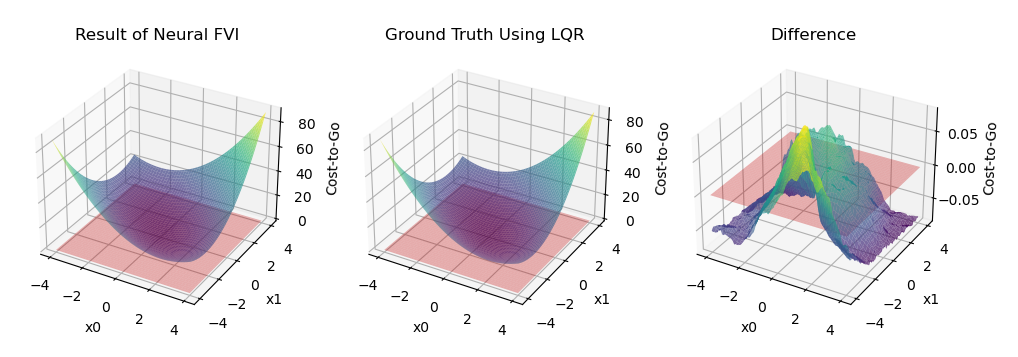
\includegraphics[width=0.9\linewidth]{images/approxdp-NN-FVI} 

}

\caption{Comparison between the result of NN-based FVI and ground truth}\label{fig:double-integrator-NN-example}
\end{figure}

The figure shows that the approximation performance of NN is pretty good. Simulation experiments also shows that the corresponding controller could successfully regulate the system at \((0,0)\).

You can see the code \href{https://github.com/ComputationalRobotics/OptimalControlEstimation-Examples/tree/main/Neural-FVI}{here}.
\end{example}

\hypertarget{fitted-q-value-iteration}{%
\subsection{Fitted Q-value Iteration}\label{fitted-q-value-iteration}}

From the MDP Chapter we know there is an equivalent representation of the Bellman Optimality Equation by replacing the \(J\) value function in \eqref{eq:bellmanoptimality-fvi} with the \(Q\)-value function \(Q(x,u)\). In particular, with
\[
J^\star(x) = \min_{u \in \mathbb{U}} Q^\star(x,u)
\]
substituted into \eqref{eq:bellmanoptimality-fvi}, we obtain the Bellman Optimality Equation in \(Q^\star(x,u)\):
\begin{equation}
Q^\star(x,u) =  g(x,u) + \mathbb{E}_w \left\{ \min_{u' \in \mathbb{U}} Q^\star(f(x,u,w),u') \right\}.
\label{eq:bellmanoptimality-fqi}
\end{equation}
We can then use the same idea to approximate \(Q^\star(x,u)\) as
\[
\tilde{Q}(x,u,r)
\]
with \(r \in \mathbb{R}^d\) a parameter vector. By iteratively evaluating the right-hand side of \eqref{eq:bellmanoptimality-fqi}, we obtain the algoithm known as \emph{fitted \(Q\)-value iteration} (FQI).

For example, we can similarly adopt the linear feature parameterization and set
\[
\tilde{Q}(x,u,r) = \phi(x,u)^T r,
\]
where \(\phi(x,u)\) is a known pre-selected feature vector. Then at the \(k\)-th iteration of FQI, we perform two subroutines.

\textbf{Value update}. We sample a number of state-control pairs \(\{(x_k^s,u_k^s) \}_{s=1}^q\) and evaluate the right-hand side of the Bellman optimality equation \eqref{eq:bellmanoptimality-fqi}:
\begin{equation}
\beta_k^s \leftarrow g(x_k^s,u_k^s) + \mathbb{E}_w \left\{ \min_{u' \in \mathbb{U}} \tilde{Q}(f(x_k^s,u_k^s,w),u',r^{(k)}) \right\}, \quad \forall s = 1,\dots,q.
\label{eq:fqi-value-update}
\end{equation}
Again, if \(u\) lives in a finite space, or the minimization is convex, the above value update can be solved exactly.

\textbf{Parameter update}. We update the parameter vector using the updated values \(\{ \beta_k^s \}_{s=1}^q\):
\begin{equation}
r^{(k+1)} \leftarrow \arg\min_{r \in \mathbb{R}^d} \sum_{s=1}^q \left( \tilde{Q}(x_k^s,u_k^s,r) - \beta_k^s \right)^2,
\label{eq:fqi-parameter-update}
\end{equation}
which is a least squares problem that can be solved in closed form.

Let us apply FQI to the same double integrator example.

\begin{example}[Fitted Q-value Iteration for Double Integrator]
\protect\hypertarget{exm:fqidoubleintegrator}{}\label{exm:fqidoubleintegrator}Consider the same double integrator dynamics in Example \ref{exm:feature-double-integrator}.

From the LQR solution we know the optimal \(Q\)-value function is
\begin{align}
Q^\star(x,u) &= x^T Q x + u^T R u + (Ax + Bu)^T S (Ax + Bu) \\
&= \begin{bmatrix} x \\ u \end{bmatrix}^T 
\underbrace{\begin{bmatrix} A^T S A + Q & A^T S B \\
B^T S A & B^T S B + R \end{bmatrix}}_{M_{\mathrm{LQR}}} \begin{bmatrix} x \\ u \end{bmatrix},
\end{align}
where \(M_{\mathrm{LQR}}\) is
\[
M_{\mathrm{LQR}} = \begin{bmatrix}
27.2640 & 32.0300 & 0.3176 \\
32.0300 & 86.6889 & 0.8627 \\
0.3176 & 0.8627 & 1.0086 
\end{bmatrix}.
\]

Let us apply FQI to see if we get the same solution. We parametrize
\begin{align}
\tilde{Q}(x,u) &= \begin{bmatrix} x \\ u \end{bmatrix}^T \begin{bmatrix}
M_1 & M_2 & M_3 \\
M_2 & M_4 & M_5 \\
M_3 & M_5 & M_6 
\end{bmatrix} \begin{bmatrix} x \\ u \end{bmatrix} \\
&= \begin{bmatrix} x_1^2 & 2 x_1 x_2 & 2x_1 u & x_2^2 & 2x_2 u & u^2 \end{bmatrix} \begin{bmatrix} M_1 \\ M_2 \\ M_3 \\ M_4 \\ M_5 \\ M_6 \end{bmatrix}.
\end{align}

At the \(k\)-th FQI iteration, we are given \(M^{(k)}\). Suppose we sample \((x_k, u_k)\), then the value update step needs to solve \eqref{eq:fqi-value-update}, which reads:
\[
\beta_k = g(x_k, u_k) + \min_{u'} \underbrace{\begin{bmatrix} A x_k + B u_k \\ u' \end{bmatrix}^T M^{(k)} \begin{bmatrix} A x_k + B u_k \\ u' \end{bmatrix}}_{\psi(u')}.
\]
The objective function \(\psi(u')\) can be shown to be quadratic:
\[
\psi(u') = (Lu' + a_k)^T M^{(k)} (Lu' + a_k), \quad L = \begin{bmatrix} 0 \\ 1 \end{bmatrix}, a_k = \begin{bmatrix} A x_k + B u_k \\ 0 \end{bmatrix}.
\]
Therefore, we can solve \(u'\) in closed-form
\[
u' = - (L^T M^{(k)} L)^{-1} L^T M^{(k)} a_k.
\]

Applying FQI with the closed-form update above, we get
\[
M_{\mathrm{FQI}} = \begin{bmatrix}
27.2640 & 32.0300 & 0.3176 \\
32.0300 & 86.6889 & 0.8627 \\
0.3176 & 0.8627 & 1.0086 
\end{bmatrix},
\]
which is exactly the same as the solution obtained from LQR.

You can play with the code \href{https://github.com/ComputationalRobotics/OptimalControlEstimation-Examples/blob/main/LQR_FQI_Example.m}{here}.
\end{example}

\hypertarget{deep-q-network}{%
\subsection{Deep Q Network}\label{deep-q-network}}

Although we have only tested FVI and FQI on the simple double integrator linear system, these algoithms are really not so different from the state-of-the-art reinforcement learning algoithms. For example, the core of the seminal work Deep \(Q\)-Network (DQN) \citep{mnih15nature-dqn} is to use a deep neural network to parameterize the \(Q\)-value function. Of course the DQN work has used other clever ideas to make it work in practice, such as experience replay, but the essence is fitted \(Q\)-value iteration.

You can find a good explanation of DQN in this \href{https://www.tensorflow.org/agents/tutorials/0_intro_rl}{tutorial}, and a practical step-by-step Pytorch implementation that \href{https://pytorch.org/tutorials/intermediate/reinforcement_q_learning.html}{applies DQN on the cart-pole system}.

\hypertarget{deep-shallow}{%
\subsection{Deep + Shallow}\label{deep-shallow}}

Combine the rich features of DQN with the stable learning of FQI \citep{levine17neurips-shallow}.

\hypertarget{trajectory-optimization}{%
\section{Trajectory Optimization}\label{trajectory-optimization}}

Consider a continuous-time optimal control problem (OCP) in full generality
\begin{equation} 
\begin{split}
\min_{u(t), t \in [0,T]} & \quad  g_T(x(T)) + \int_{t = 0}^T g(x(t),u(t)) dt \\
\text{subject to} & \quad \dot{x} = f(x(t),u(t)) \\
& \quad x(0) = x_0 \\
& \quad (x(t),u(t)) \in \mathcal{X} \times \mathcal{U} \\
& \quad \phi_i (x(t),u(t)) \geq 0, i=1,\dots,q.
\end{split}
\label{eq:constrained-optimal-control}
\end{equation}
where \(g_T\) the terminal cost, \(g\) the running cost, \(x_0\) the initial condition, \(\mathcal{X}\) the state constraint set, \(\mathcal{U}\) the control constraint set, and \(\{ \phi_i \}_{i=1}^q\) are general state-control constraints. We assume that the state constraint set \(\mathcal{X}\) and control constraint set \(\mathcal{U}\) can be described by a finite set of inequalities, i.e.,
\[
\mathcal{X} = \{x \in \mathbb{R}^n \mid c^x_i(x) \geq 0, i =1,\dots,q_x\}, \quad \mathcal{U} = \{u \in \mathbb{R}^m \mid c^u_i(u) \geq 0, i = 1,\dots,q_u \}.
\]
Assume that all functions are differentiable.

Our goal is to ``transcribe'' the infinite-dimensional continuous-time optimization \eqref{eq:constrained-optimal-control} into a \emph{nonlinear programming problem} (NLP) of the following form
\begin{equation}
\begin{split}
\min_{v \in \mathbb{R}^{n_v}} & \quad c(v) \\
\text{subject to} & \quad c_{\text{eq},i}(v) = 0, i =1,\dots, n_{\text{eq}} \\
& \quad c_{\text{ineq},i}(v) \geq 0, i=1,\dots,n_{\text{ineq}},
\end{split}
\label{eq:ocp-nonlinear-programming}
\end{equation}
where \(v\) is a finite-dimensional vector variable to be optimized, \(c, c_{\text{eq},i}, c_{\text{ineq},i}\) are (continuously differentiable) objective and constraint functions. Once we have done the transcription from \eqref{eq:constrained-optimal-control} to \eqref{eq:ocp-nonlinear-programming}, then we have a good number of numerical optimization algorithms at our disposal. For example, the Matlab \href{https://www.mathworks.com/help/optim/ug/fmincon.html}{\texttt{fmincon}} provides a nice interface to many such algorithms, e.g., interior-point method and sequential quadratic programming. You have already played with a simple example of \texttt{fmincon} in Exercise \ref{exr:polygoninsidecircle}. Other well-implemented NLP algorithms include \href{https://github.com/coin-or/Ipopt}{IPOPT} and \href{http://www.sbsi-sol-optimize.com/asp/sol_product_snopt.htm}{SNOPT}. However, usually the Matlab \texttt{fmincon} gives a decent start point for trying out different algorithms before moving to commercial solvers such as SNOPT. For a more comprehensive understanding about how NLP algoithms work under the hood, I suggest reading \citep{nocedal99book-numerical}.

Before we talk about how to transcribe the OCP into an NLP, let us use a simple example to get a taste of \texttt{fmincon}.

\begin{example}[Fire a Canon with fmincon]
\protect\hypertarget{exm:fmincon-example}{}\label{exm:fmincon-example}On a 2D plane, suppose we have a canon at the origin \((0,0)\), and we want to fire the canon, with control over the initial velocity \((v_1, v_2)\), so that the canon ball hits the target location \((10,10)\).

From our basic physics knowledge, we know the trajectory of the canon ball is described by
\[
\begin{cases}
x_1(t) = v_1 t \\
x_2(t) = v_2 t - \frac{1}{2}g t^2,
\end{cases}
\]
where \(g\) is the gravity constant.

With the trajectory of the canon ball written above, we can formulate our nonlinear programming problem (NLP) as:
\begin{equation}
\begin{split}
\min_{v_1, v_2, T} & \quad \frac{1}{2} (v_1^2 + v_2^2) \\
\text{subject to} & \quad v_1, v_2, T \geq 0 \\
& \quad x_1(T) = v_1 T = 10 \\
& \quad x_2(T) = v_2 T - \frac{1}{2}g T^2 = 10 
\end{split}
\label{eq:fire-canon}
\end{equation}
where our unknown variables are the initial velocities and the time \(T\) at which the canon ball hits the target. In the NLP \eqref{eq:fire-canon}, the first constraint asks all our varaibles to be nonnegative, the second and third constraints enforce the canon ball to hit the target.

The following script formulates the NLP \eqref{eq:fire-canon} in matlab.

\begin{Shaded}
\begin{Highlighting}[]
\VariableTok{clc}\OperatorTok{;} \VariableTok{clear}\OperatorTok{;} \VariableTok{close} \VariableTok{all}\OperatorTok{;}
\VariableTok{g} \OperatorTok{=} \FloatTok{9.8}\OperatorTok{;}
\VariableTok{x0} \OperatorTok{=}\NormalTok{ [}\FloatTok{0}\OperatorTok{;}\FloatTok{0}\OperatorTok{;}\FloatTok{1}\NormalTok{]}\OperatorTok{;} \CommentTok{\% initial guess of the solution}
\CommentTok{\% define objective function}
\VariableTok{obj} \OperatorTok{=} \OperatorTok{@}\NormalTok{(}\VariableTok{x}\NormalTok{) }\VariableTok{objective}\NormalTok{(}\VariableTok{x}\NormalTok{)}\OperatorTok{;}
\CommentTok{\% define nonlinear constraints}
\VariableTok{nonlincon} \OperatorTok{=} \OperatorTok{@}\NormalTok{(}\VariableTok{x}\NormalTok{) }\VariableTok{nonlinear\_con}\NormalTok{(}\VariableTok{x}\OperatorTok{,}\VariableTok{g}\NormalTok{)}\OperatorTok{;}
\CommentTok{\% define options for fmincon}
\VariableTok{options} \OperatorTok{=} \VariableTok{optimoptions}\NormalTok{(}\SpecialStringTok{\textquotesingle{}fmincon\textquotesingle{}}\OperatorTok{,}\SpecialStringTok{\textquotesingle{}Algorithm\textquotesingle{}}\OperatorTok{,}\SpecialStringTok{\textquotesingle{}interior{-}point\textquotesingle{}}\OperatorTok{,...}
    \SpecialStringTok{\textquotesingle{}SpecifyObjectiveGradient\textquotesingle{}}\OperatorTok{,}\VariableTok{true}\OperatorTok{,}\SpecialStringTok{\textquotesingle{}SpecifyConstraintGradient\textquotesingle{}}\OperatorTok{,}\VariableTok{true}\OperatorTok{,...}
    \SpecialStringTok{\textquotesingle{}checkGradients\textquotesingle{}}\OperatorTok{,}\VariableTok{false}\NormalTok{)}\OperatorTok{;}
\CommentTok{\% call fmincon}
\NormalTok{[}\VariableTok{xopt}\OperatorTok{,}\VariableTok{fopt}\OperatorTok{,\textasciitilde{},}\VariableTok{out}\NormalTok{] }\OperatorTok{=} \VariableTok{fmincon}\NormalTok{(}\VariableTok{obj}\OperatorTok{,}\VariableTok{x0}\OperatorTok{,...} \CommentTok{\% objective and initial guess}
    \OperatorTok{{-}}\VariableTok{eye}\NormalTok{(}\FloatTok{3}\NormalTok{)}\OperatorTok{,}\VariableTok{zeros}\NormalTok{(}\FloatTok{3}\OperatorTok{,}\FloatTok{1}\NormalTok{)}\OperatorTok{,...} \CommentTok{\% linear inequality constraints}
\NormalTok{    []}\OperatorTok{,}\NormalTok{[]}\OperatorTok{,...} \CommentTok{\% no linear equality constraints}
\NormalTok{    []}\OperatorTok{,}\NormalTok{[]}\OperatorTok{,...} \CommentTok{\% no upper and lower bounds}
    \VariableTok{nonlincon}\OperatorTok{,...} \CommentTok{\% nonlinear constraints}
    \VariableTok{options}\NormalTok{)}\OperatorTok{;}
\VariableTok{fprintf}\NormalTok{(}\StringTok{"Maximum constraint violation: \%3.2f.\textbackslash{}n"}\OperatorTok{,}\VariableTok{out}\NormalTok{.}\VariableTok{constrviolation}\NormalTok{)}\OperatorTok{;}
\VariableTok{fprintf}\NormalTok{(}\StringTok{"Objective: \%3.2f.\textbackslash{}n"}\OperatorTok{,}\VariableTok{fopt}\NormalTok{)}\OperatorTok{;}
\CommentTok{\% plot the solution}
\VariableTok{T} \OperatorTok{=} \VariableTok{xopt}\NormalTok{(}\FloatTok{3}\NormalTok{)}\OperatorTok{;}
\VariableTok{t} \OperatorTok{=} \FloatTok{0}\OperatorTok{:}\FloatTok{0.01}\OperatorTok{:}\VariableTok{T}\OperatorTok{;}
\VariableTok{xt} \OperatorTok{=} \VariableTok{xopt}\NormalTok{(}\FloatTok{1}\NormalTok{)}\OperatorTok{*}\VariableTok{t}\OperatorTok{;}
\VariableTok{yt} \OperatorTok{=} \VariableTok{xopt}\NormalTok{(}\FloatTok{2}\NormalTok{)}\OperatorTok{*}\VariableTok{t} \OperatorTok{{-}} \FloatTok{0.5}\OperatorTok{*}\VariableTok{g}\OperatorTok{*}\NormalTok{(}\VariableTok{t}\OperatorTok{.\^{}}\FloatTok{2}\NormalTok{)}\OperatorTok{;}
\VariableTok{figure}\OperatorTok{;}
\VariableTok{plot}\NormalTok{(}\VariableTok{xt}\OperatorTok{,}\VariableTok{yt}\OperatorTok{,}\SpecialStringTok{\textquotesingle{}LineWidth\textquotesingle{}}\OperatorTok{,}\FloatTok{2}\NormalTok{)}\OperatorTok{;}
\VariableTok{hold} \VariableTok{on}
\VariableTok{scatter}\NormalTok{(}\FloatTok{10}\OperatorTok{,}\FloatTok{10}\OperatorTok{,}\FloatTok{100}\OperatorTok{,}\StringTok{"red"}\OperatorTok{,}\SpecialStringTok{\textquotesingle{}filled\textquotesingle{}}\OperatorTok{,}\SpecialStringTok{\textquotesingle{}diamond\textquotesingle{}}\NormalTok{)}\OperatorTok{;}
\VariableTok{axis} \VariableTok{equal}\OperatorTok{;} \VariableTok{grid} \VariableTok{on}\OperatorTok{;}
\VariableTok{xlabel}\NormalTok{(}\SpecialStringTok{\textquotesingle{}$x\_1(t)$\textquotesingle{}}\OperatorTok{,}\SpecialStringTok{\textquotesingle{}FontSize\textquotesingle{}}\OperatorTok{,}\FloatTok{24}\OperatorTok{,}\SpecialStringTok{\textquotesingle{}Interpreter\textquotesingle{}}\OperatorTok{,}\SpecialStringTok{\textquotesingle{}latex\textquotesingle{}}\NormalTok{)}\OperatorTok{;}
\VariableTok{ylabel}\NormalTok{(}\SpecialStringTok{\textquotesingle{}$x\_2(t)$\textquotesingle{}}\OperatorTok{,}\SpecialStringTok{\textquotesingle{}FontSize\textquotesingle{}}\OperatorTok{,}\FloatTok{24}\OperatorTok{,}\SpecialStringTok{\textquotesingle{}Interpreter\textquotesingle{}}\OperatorTok{,}\SpecialStringTok{\textquotesingle{}latex\textquotesingle{}}\NormalTok{)}\OperatorTok{;}
\VariableTok{ax} \OperatorTok{=} \VariableTok{gca}\OperatorTok{;} \VariableTok{ax}\NormalTok{.}\VariableTok{FontSize} \OperatorTok{=} \FloatTok{20}\OperatorTok{;}
\CommentTok{\%\% helper functions}
\KeywordTok{function}\NormalTok{ [}\VariableTok{f}\OperatorTok{,}\VariableTok{df}\NormalTok{] }\OperatorTok{=} \VariableTok{objective}\NormalTok{(}\VariableTok{x}\NormalTok{)}
\CommentTok{\% x is our decision variable: [v1, v2, T]}
\CommentTok{\% objective function}
\VariableTok{f} \OperatorTok{=} \FloatTok{0.5} \OperatorTok{*}\NormalTok{ (}\VariableTok{x}\NormalTok{(}\FloatTok{1}\NormalTok{)}\OperatorTok{\^{}}\FloatTok{2} \OperatorTok{+} \VariableTok{x}\NormalTok{(}\FloatTok{2}\NormalTok{)}\OperatorTok{\^{}}\FloatTok{2}\NormalTok{)}\OperatorTok{;}
\CommentTok{\% gradient of the objective function (optional)}
\VariableTok{df} \OperatorTok{=}\NormalTok{ [}\VariableTok{x}\NormalTok{(}\FloatTok{1}\NormalTok{)}\OperatorTok{;} \VariableTok{x}\NormalTok{(}\FloatTok{2}\NormalTok{)}\OperatorTok{;} \FloatTok{0}\NormalTok{]}\OperatorTok{;} \CommentTok{\% column vector}
\KeywordTok{end}

\KeywordTok{function}\NormalTok{ [}\VariableTok{c}\OperatorTok{,}\VariableTok{ceq}\OperatorTok{,}\VariableTok{dc}\OperatorTok{,}\VariableTok{dceq}\NormalTok{] }\OperatorTok{=} \VariableTok{nonlinear\_con}\NormalTok{(}\VariableTok{x}\OperatorTok{,}\VariableTok{g}\NormalTok{)}
\CommentTok{\% no inequality constraints}
\VariableTok{c} \OperatorTok{=}\NormalTok{ []}\OperatorTok{;} \VariableTok{dc} \OperatorTok{=}\NormalTok{ []}\OperatorTok{;}
\CommentTok{\% two equality constraints}
\VariableTok{ceq} \OperatorTok{=}\NormalTok{ [}\VariableTok{x}\NormalTok{(}\FloatTok{1}\NormalTok{)}\OperatorTok{*}\VariableTok{x}\NormalTok{(}\FloatTok{3}\NormalTok{)}\OperatorTok{{-}}\FloatTok{10}\OperatorTok{;}
       \VariableTok{x}\NormalTok{(}\FloatTok{2}\NormalTok{)}\OperatorTok{*}\VariableTok{x}\NormalTok{(}\FloatTok{3}\NormalTok{)}\OperatorTok{{-}}\FloatTok{0.5}\OperatorTok{*}\VariableTok{g}\OperatorTok{*}\VariableTok{x}\NormalTok{(}\FloatTok{3}\NormalTok{)}\OperatorTok{\^{}}\FloatTok{2}\OperatorTok{{-}}\FloatTok{10}\NormalTok{]}\OperatorTok{;}
\CommentTok{\% explicit gradient of ceq}
\VariableTok{dceq} \OperatorTok{=}\NormalTok{ [}\VariableTok{x}\NormalTok{(}\FloatTok{3}\NormalTok{)}\OperatorTok{,} \FloatTok{0}\OperatorTok{;}
        \FloatTok{0}\OperatorTok{,} \VariableTok{x}\NormalTok{(}\FloatTok{3}\NormalTok{)}\OperatorTok{;}
        \VariableTok{x}\NormalTok{(}\FloatTok{1}\NormalTok{)}\OperatorTok{,} \VariableTok{x}\NormalTok{(}\FloatTok{2}\NormalTok{)}\OperatorTok{{-}}\VariableTok{g}\OperatorTok{*}\VariableTok{x}\NormalTok{(}\FloatTok{3}\NormalTok{)]}\OperatorTok{;}
\KeywordTok{end}
\end{Highlighting}
\end{Shaded}

Running the code above, we get the following trajectory

\begin{figure}

{\centering 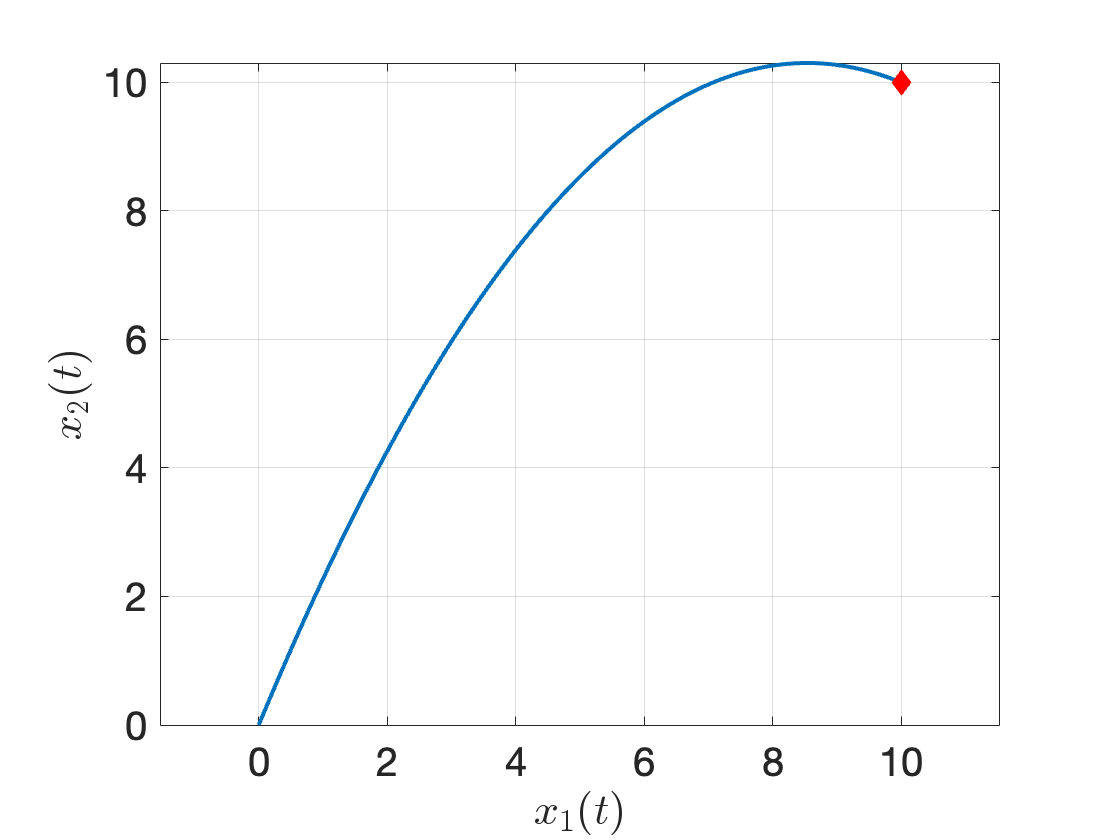
\includegraphics[width=0.7\linewidth]{images/canon_ball} 

}

\caption{Trajectory of the canon ball obtained from fmincon.}\label{fig:fire-canon-ball}
\end{figure}

What if you change the initial guess to \texttt{fmincon}, or add more constraints? Feel free to play with the code \href{https://github.com/ComputationalRobotics/OptimalControlEstimation-Examples/blob/main/fire_canon_ball_fmincon.m}{here}.
\end{example}

It turns out there are multiple different ways to transcribe the optimal control problem \eqref{eq:constrained-optimal-control} as the nonlinear programming problem \eqref{eq:ocp-nonlinear-programming}. In the following, we will introduce three different formulations, direct single shooting, direct multiple shooting, and direct collocation.

\hypertarget{direct-single-shooting}{%
\subsection{Direct Single Shooting}\label{direct-single-shooting}}

In direct single shooting, we transcribe the OCP to the NLP by only optimizing a sequence of control values, with the intuition being that the state values are functions of the controls by invoking the system dynamics. In particular, we follow the procedure below.

\textbf{Time discretization}. We first discretize the total time window \([0,T]\) into a set of \(N\) intervals:
\[
0 = t_0 \leq t_1 \leq \dots \leq t_k \leq t_{k+1} \leq \dots \leq t_N = T.
\]
We denote
\[
h_k = t_{k+1} - t_k
\]
as the length of the \(k\)-th time interval.

\textbf{Piece-wise constant control}. We will approximate the continuous-time control signal \(u(t)\) as a piece-wise constant function, i.e.,
\[
u(t) = u_k, \forall t \in [t_k, t_{k+1}).
\]
This is shown in Fig. \ref{fig:direct-single-shooting}. Let us collect all the constant control values as our decision variable to be optimized
\begin{equation}
v = \begin{bmatrix} u_0 \\ u_1 \\ \vdots \\ u_{N-1} \end{bmatrix} \in \mathbb{R}^{N m}.
\label{eq:direct-single-shooting-v}
\end{equation}
This \(v\) will be our variable in the NLP \eqref{eq:ocp-nonlinear-programming}. Note that \(v\) has dimension \(N m\).

\begin{figure}

{\centering 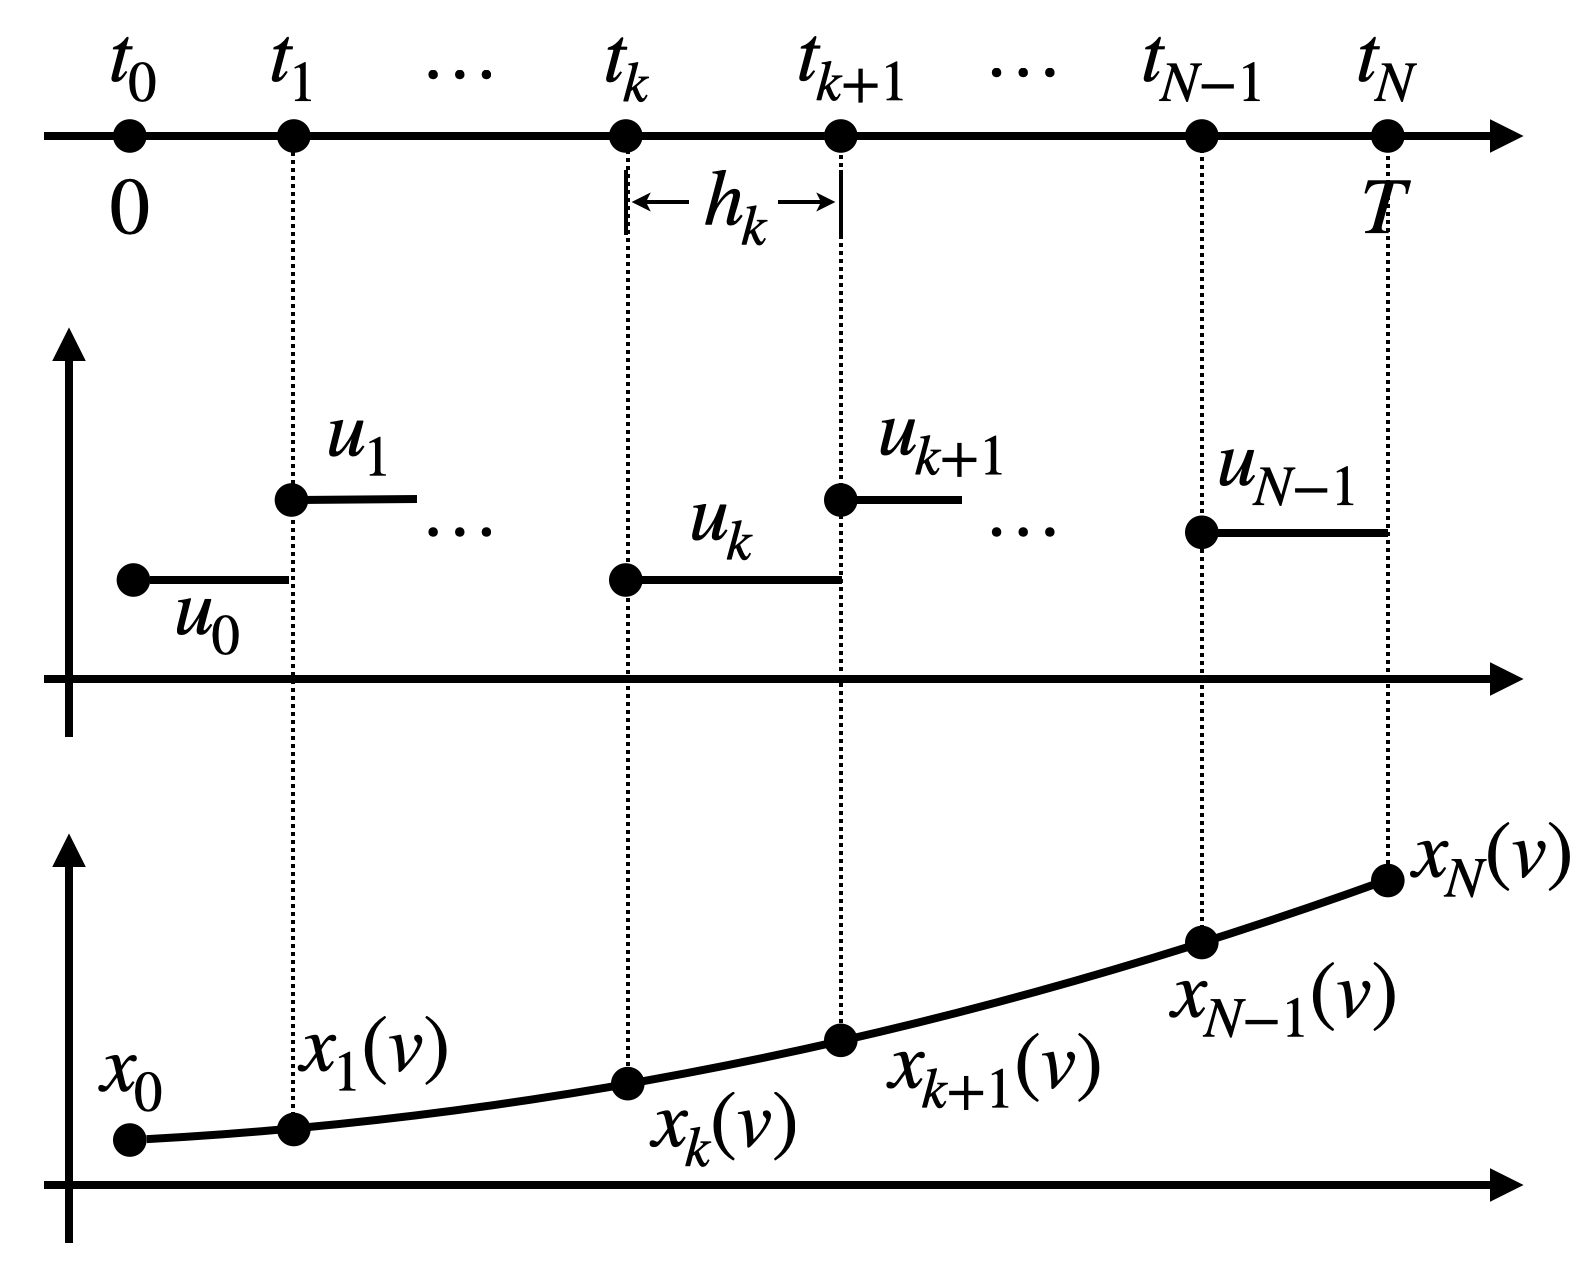
\includegraphics[width=0.6\linewidth]{images/direct_single_shooting} 

}

\caption{Direct single shooting.}\label{fig:direct-single-shooting}
\end{figure}

\textbf{Dynamics integration}. It is clear that once \(v\) in \eqref{eq:direct-single-shooting-v}, i.e., the set of controls, is determined, then the state trajectory \(x(t)\) is also uniquely determined by the initial condition \(x(0) = x_0\) and the dynamics
\[
\dot{x}(t) = f(x(t),u(t)).
\]
In order to enforce the state constraint \(x(t) \in \mathcal{X}\), we will enforce the values of \(x\) at \(t_0,t_1,\dots,t_N\), i.e., \(x_k = x(t_k)\), to lie in the constraint set \(\mathcal{X}\). To do so, we need to integrate the dynamics. When the dynamics is linear, this integration can be done in closed form:
\[
x_{k+1} = x_k + \int_{\tau=t_k}^{t_k + h_k} A x(\tau) + B u(\tau) d\tau = e^{Ah_k} x_k + A^{-1}(e^{Ah_k} - I) B u_k.
\]
By running the above equation from \(k=0\) to \(k=N-1\), we obtain the values of \(x_k,k=1,\dots,N\) as functions of the control vectors \(v\), shown in Fig. \ref{fig:direct-single-shooting}. When the dynamics is nonlinear, we will need to perform the dynamics integration using numerical integration. One of the most well known family of integrators is called \href{https://en.wikipedia.org/wiki/Runge\%E2\%80\%93Kutta_methods\#Adaptive_Runge\%E2\%80\%93Kutta_methods}{``Runge-Kutta methods''}. Among the family of methods, RK45 is perhaps the most popular one. We now briefly describe how a fourth-order RK integrator, i.e., RK4, works. Suppose we have already computed \(x_k\), and we want to integrate the dynamics to obtain \(x_{k+1}\). The RK4 integrator first computes the time derivatives at a sequence of four points:
\begin{align}
\alpha_1 &= f(x_k, u_k) \\
\alpha_2 &= f\left( x_k + \frac{1}{2} h_k \alpha_1, u_k \right) \\
\alpha_3 &= f\left( x_k + \frac{1}{2} h_k \alpha_2, u_k \right) \\
\alpha_4 &= f\left( x_k + h_k \alpha_3, u_k \right).
\end{align}
Then we can obtain \(x_{k+1}\) via a weighted sum of the \(\alpha_i\)'s
\begin{equation}
x_{k+1} = x_k + \frac{1}{6} h_k \left( \alpha_1 + 2 \alpha_2 + 2 \alpha_3 + \alpha_4 \right) = \text{RK4}(x_k, u_k).
\label{eq:RK4-integrator}
\end{equation}
Notice that a naive integrator would just perform \(x_{k+1} = x_k + h_k \alpha_1\) without querying the gradients at three other points. The nice property of RK4 is that it leads to better accuracy than the naive integration. Writing the RK4 integrator recursively, we obtain
\[
x_{k+1} = \text{RK4}(x_k, u_k) = \text{RK4}(\text{RK4}(x_{k-1},u_{k-1}),u_k) = \text{RK4}(\text{RK4}(...(x_0,u_0))...u_k),
\]
where RK4 is invoked for \(k+1\) times. Clearly, each \(x_k\) is a complicated function of the sequence of controls \(v\) and the initial state \(x_0\). We will write \(x_k(v)\) to make this explict, as shown in Fig. \ref{fig:direct-single-shooting}.

\textbf{Objective approximation}. We can approximate the objective of the OCP \eqref{eq:constrained-optimal-control} using trapezoidal integration:
\[
g_T(x(T)) + \int_{t=0}^T g(x(t),u(t)) dt \approx g_T(x_N(v)) + \sum_{k=0}^{N-1} \frac{h_k}{2}(g(x_k(v),u_k) + g(x_{k+1}(v),u_{k+1})).
\]

\textbf{Summary}. In summary, the transcribed NLP for the optimal control problem using direct single shooting would be
\begin{equation}
\begin{split}
\min_{v = (u_0,\dots,u_{N-1})} & \quad g_T(x_N(v)) + \sum_{k=0}^{N-1} \frac{g(x_k(v),u_k) + g(x_{k+1}(v), u_{k+1})}{2} h_k \\
\text{subject to} & \quad c^u_i(u_k) \geq 0, i=1,\dots,q_u, \quad k=0,\dots,N-1 \\
& \quad c^x_i(x_k(v)) \geq 0, i=1,\dots,q_x, \quad k=1,\dots,N \\
& \quad \phi_i(x_k(v),u_k) \geq 0, i=1,\dots, q, \quad k=0,\dots,N.
\end{split}
\label{eq:ocp-direct-single-shooting}
\end{equation}

\textbf{Pros and Cons}. The advantage of using direct single shooting to transcribe the OCP is clear: it leads to fewer variables because the only decision variables in \eqref{eq:ocp-direct-single-shooting} are the sequence of controls. In other transcription methods, the decision variable of the NLP typically involves the states as well. The disadvantage of direct single shooting is the complication of the function \(x_k(v)\) caused by numerical integrators such as RK4. Even though the original continuous-time dynamics \(f(x,u)\) may be simple, the RK4 function can be highly complicated due to evaluating \(\dot{x}\) at multiple other locations. Moreover, the recursion of the RK4 operator makes this complication even worse.

Let us try the RK4 simulator for a simple example.

\begin{example}[Propagation of Nonlinearities]
\protect\hypertarget{exm:RK4-simulation}{}\label{exm:RK4-simulation}

Consider the following dynamics
\[
x = \begin{bmatrix} x_1 \\ x_2 \\ x_3 \end{bmatrix}, \quad 
\dot{x} = \begin{bmatrix} 
10(x_2 - x_1) \\
x_1(u - x_3) - x_2 \\
x_1 x_2 - 3 x_3 
\end{bmatrix}
\]
where \(u\) is a single scalar control. We are interested in running the RK4 simulator for \(100\) seconds (with \(h_k = 0.01\) for all \(k\)) at \(x_0 = [1,0,0]^T\) with \(u\) varying from \(0\) to \(100\), and see how the nonlinearities propagate.

Fig. \ref{fig:RK4-simulate} plots \(x\) as a function of \(u\). We can clearly see the nonlinearities getting worse due to RK4.

You can play with the code \href{https://github.com/ComputationalRobotics/OptimalControlEstimation-Examples/blob/main/RK4_example.m}{here}.

\begin{figure}

{\centering 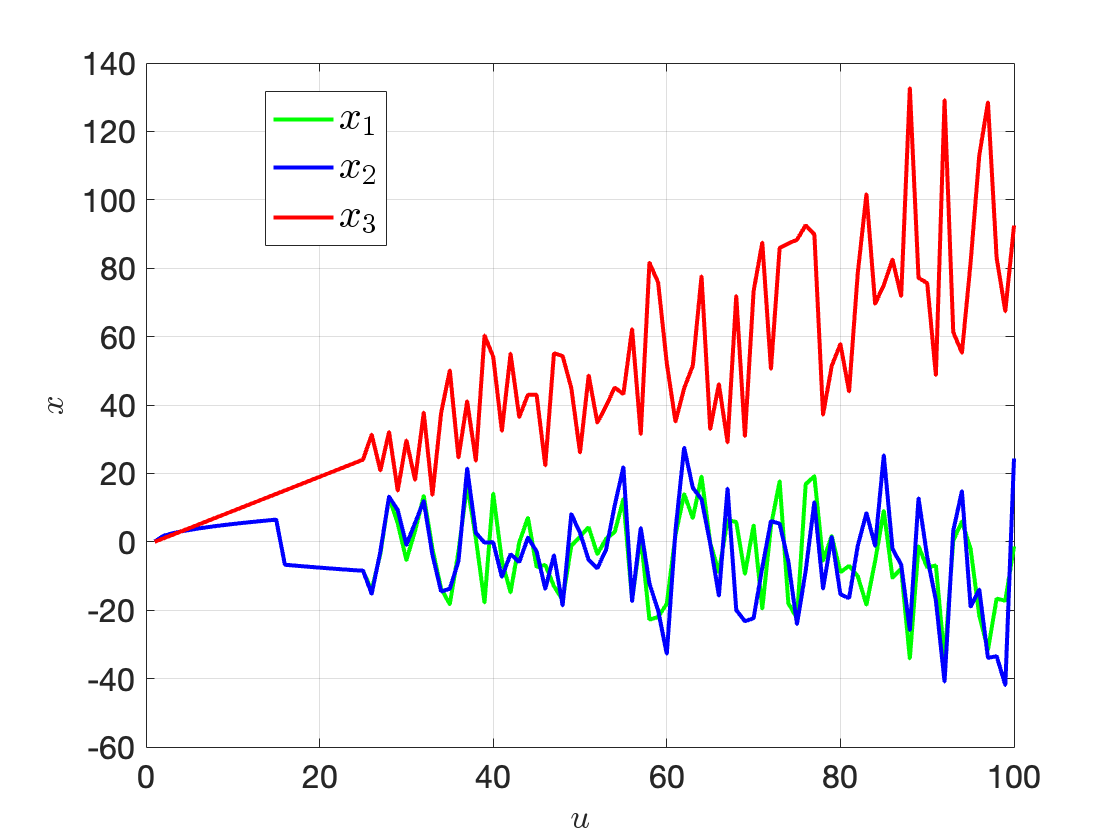
\includegraphics[width=0.6\linewidth]{images/RK4-sim} 

}

\caption{RK4 simulation.}\label{fig:RK4-simulate}
\end{figure}

\end{example}

\hypertarget{direct-multiple-shooting}{%
\subsection{Direct Multiple Shooting}\label{direct-multiple-shooting}}

\begin{figure}

{\centering 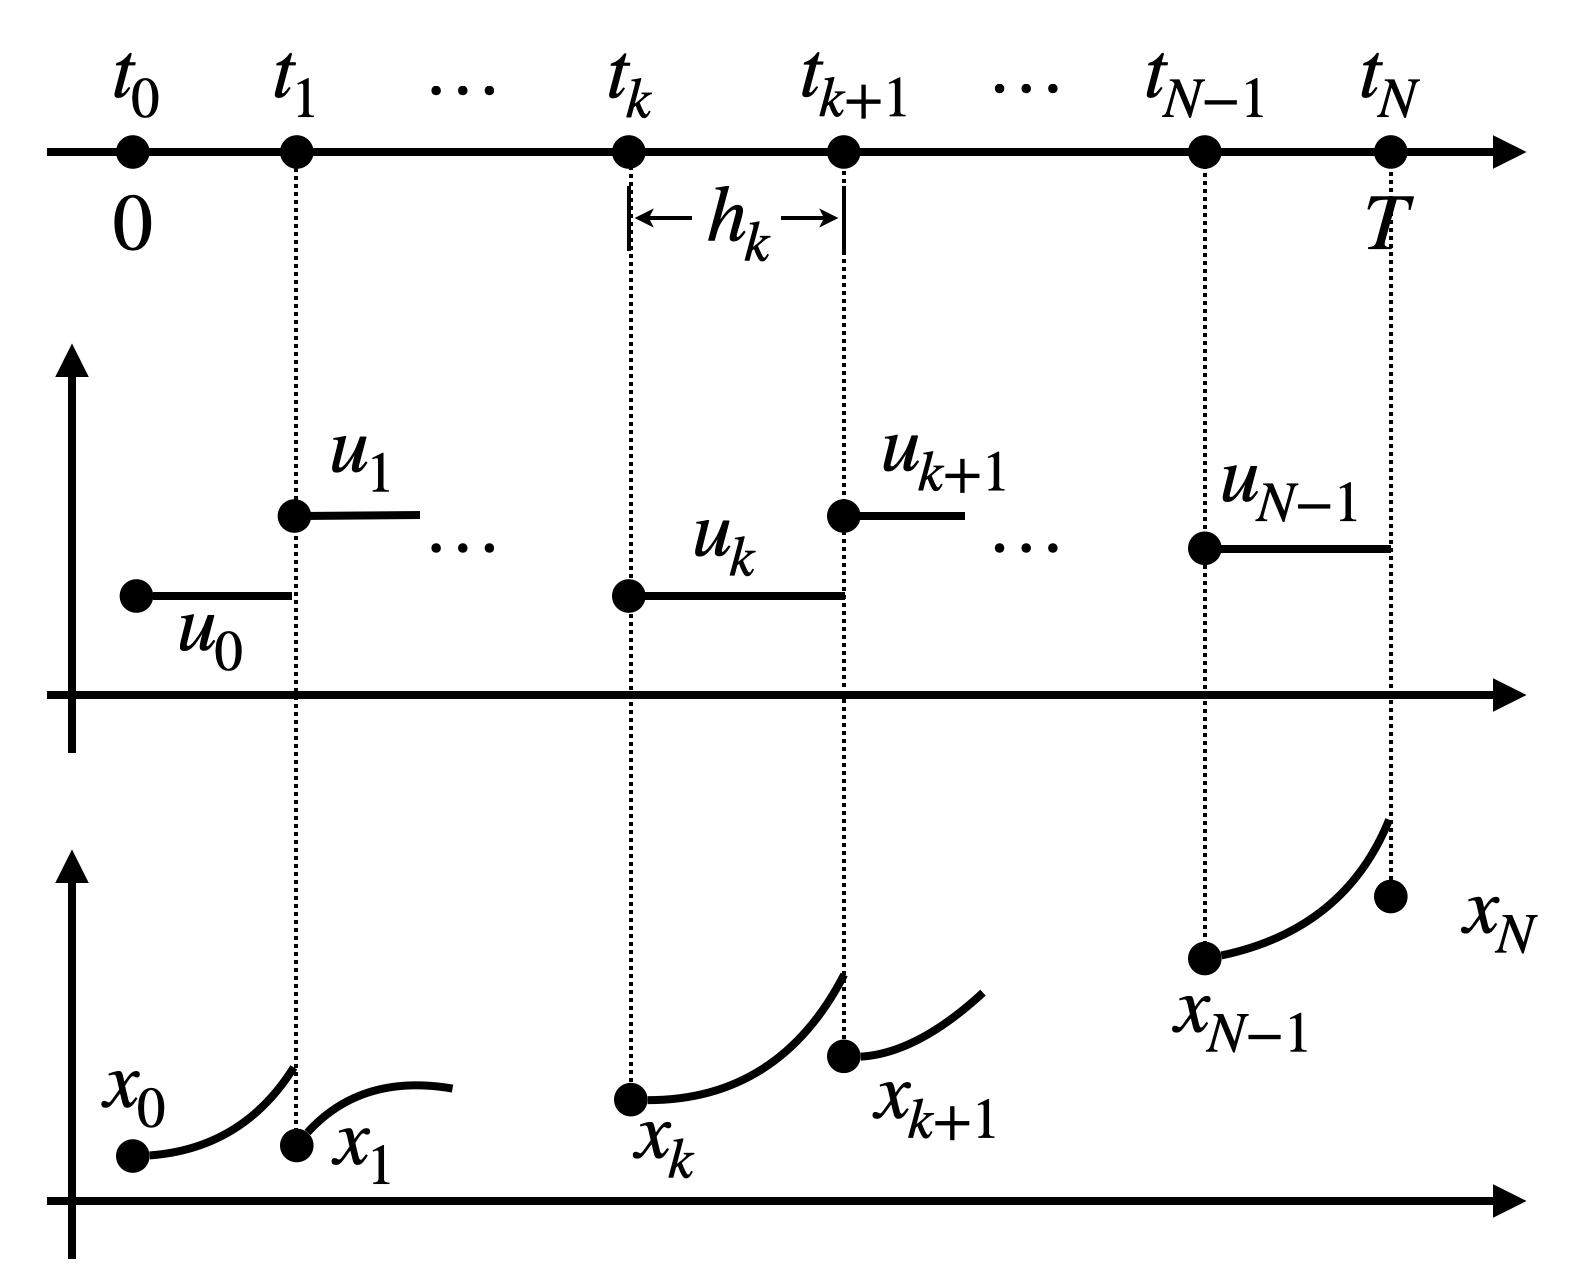
\includegraphics[width=0.6\linewidth]{images/direct_multiple_shooting} 

}

\caption{Direct multiple shooting.}\label{fig:direct-multiple-shooting}
\end{figure}

Propagation of the nonlinearities through numerical integrators motivates using \emph{direct multiple shooting} to transcribe the OCP problem into a nonlinear programming problem.

Instead of only optimizing the controls, direct multiple shooting optimizes both the controls and states. The decision variable in the NLP becomes
\[
v = \begin{bmatrix}
u_0 \\ u_1 \\ \vdots \\ u_{N-1} \\ x_1 \\ x_2 \\ \vdots \\ x_N \end{bmatrix} \in \mathbb{R}^{N(n+m)}.
\]
With the state variables also introduced in the optimization, we no longer need to recursively run the RK4 integrators. Instead, we just need to run it once and enforce
\[
x_{k+1} = \text{RK4}(x_k, u_k),
\]
i.e., the current state and the next state satisfy the dynamics constraint. This is shown in Fig. \ref{fig:direct-multiple-shooting}.

In summary, the transcribed NLP for the OCP problem using direct multiple shooting becomes
\begin{equation}
\begin{split}
\min_{v = (u_0,\dots,u_{N-1},x_1,\dots,x_N)} & \quad g_T(x_N) + \sum_{k=0}^{N-1} \frac{g(x_k,u_k) + g(x_{k+1},u_{k+1})}{2} h_k \\
\text{subject to} & \quad x_{k+1} = \text{RK4}(x_k, u_k), \quad k=0,\dots,N-1 \\
& \quad c^u_i (u_k) \geq 0, i=1,\dots,q_u, \quad k=0,\dots,N-1 \\
& \quad c^x_i(x_k) \geq 0, i=1,\dots,q_x, \quad k=1,\dots,N \\
& \quad \phi_i(x_k, u_k) \geq 0, i=1,\dots,q, \quad k=0,\dots,N.
\end{split}
\label{eq:ocp-direct-multiple-shooting}
\end{equation}

Direct multiple shooting avoids the recursion of numerical integrators such as RK4, but at the expense of introducing additional state variables in the NLP.

Let us try direct multiple shooting on the double integrator.

\begin{example}[Direct Multiple Shooting for Minimum-Time Double Integrator]
\protect\hypertarget{exm:multiple-shooting-double-integrator}{}\label{exm:multiple-shooting-double-integrator}

The double integrator has continuous-time dynamics (which you have already seen in Exercise \ref{exr:lqrconstraints}):
\[
\ddot{q} = u.
\]
In standard state-space form, the dynamics is linear
\[
x = \begin{bmatrix} q \\ \dot{q} \end{bmatrix}, \quad 
\dot{x} = \begin{bmatrix} 0 & 1 \\ 0 & 0 \end{bmatrix} x + \begin{bmatrix} 0 \\ 1 \end{bmatrix} u.
\]

Let us consider the minimum-time optimal control problem
\begin{equation}
\begin{split}
\min_{u(t),t \in [0,T]} & \quad T \\
\text{subject to} & \quad \dot{x} = A x + Bu, \quad x(0) = x_0 \\
& \quad x(T) = 0 \\
& \quad u(t) \in [-1,1], \forall t \in [0,T].
\end{split}
\end{equation}
which seeks to get from the initial condition \(x_0\) to the origin as fast as possible.

You should know from our physics intuition that the optimal controller is bang-bang, i.e., the optimal control first accelerates (deaccelerates) using the maximum control and then reverses using the opposite maximum control.

Let's see if we can obtain the optimal controller using direct multiple shooting.

In direct multiple shooting, we will optimize the control trajectory, the state trajectory, and the final time \(T\). We fix the number of intervals \(N\), and discretize \([0,T]\) evenly into \(N\) intervals, which leads to variables for the NLP as
\[
v=(T,x_0,\dots,x_{N},u_0,\dots,u_N).
\]
We can easily enforce the control constraints:
\[
u_k \in [-1,1],k=0,\dots,N,
\]
and the initial / terminal constraints
\[
x_0 = x_0, \quad x_N = 0.
\]
The only nontrivial constraint is the dynamics constraint:
\[
x_{k+1} = \text{RK4}(x_k,u_k),k=0,\dots,N-1.
\]

The following script shows how to use the Matlab integrator \texttt{ode45} to enforce the dynamics constraint.

\begin{Shaded}
\begin{Highlighting}[]
\KeywordTok{function} \VariableTok{dx} \OperatorTok{=} \VariableTok{double\_integrator}\NormalTok{(}\VariableTok{t}\OperatorTok{,}\VariableTok{states}\OperatorTok{,}\VariableTok{v}\NormalTok{)}
\CommentTok{\% return xdot at the selected times t and states, using information from v}
\CommentTok{\% assume the controls in v define piece{-}wise constant control signal}
\VariableTok{T} \OperatorTok{=} \VariableTok{v}\NormalTok{(}\FloatTok{1}\NormalTok{)}\OperatorTok{;} \CommentTok{\% final time}
\VariableTok{N} \OperatorTok{=}\NormalTok{ (}\VariableTok{length}\NormalTok{(}\VariableTok{v}\NormalTok{) }\OperatorTok{{-}} \FloatTok{1}\NormalTok{) }\OperatorTok{/} \FloatTok{3}\OperatorTok{;} \CommentTok{\% number of knot points}
\VariableTok{u\_grid} \OperatorTok{=} \VariableTok{v}\NormalTok{(}\FloatTok{2}\OperatorTok{+}\FloatTok{2}\OperatorTok{*}\VariableTok{N}\OperatorTok{:}\FloatTok{3}\OperatorTok{*}\VariableTok{N}\OperatorTok{+}\FloatTok{1}\NormalTok{)}\OperatorTok{;} \CommentTok{\% N controls}
\VariableTok{t\_grid} \OperatorTok{=} \VariableTok{linspace}\NormalTok{(}\FloatTok{0}\OperatorTok{,}\FloatTok{1}\OperatorTok{,}\VariableTok{N}\NormalTok{)}\OperatorTok{*}\VariableTok{T}\OperatorTok{;}
\VariableTok{u\_t} \OperatorTok{=} \VariableTok{interp1}\NormalTok{(}\VariableTok{t\_grid}\OperatorTok{,}\VariableTok{u\_grid}\OperatorTok{,}\VariableTok{t}\OperatorTok{,}\SpecialStringTok{\textquotesingle{}previous\textquotesingle{}}\NormalTok{)}\OperatorTok{;} \CommentTok{\% piece{-}wise constant}
\VariableTok{A} \OperatorTok{=}\NormalTok{ [}\FloatTok{0} \FloatTok{1}\OperatorTok{;} \FloatTok{0} \FloatTok{0}\NormalTok{]}\OperatorTok{;}
\VariableTok{B} \OperatorTok{=}\NormalTok{ [}\FloatTok{0}\OperatorTok{;} \FloatTok{1}\NormalTok{]}\OperatorTok{;}
\VariableTok{dx} \OperatorTok{=} \VariableTok{A} \OperatorTok{*} \VariableTok{states} \OperatorTok{+} \VariableTok{B} \OperatorTok{*} \VariableTok{u\_t}\OperatorTok{;}
\KeywordTok{end}

\KeywordTok{function}\NormalTok{ [}\VariableTok{c}\OperatorTok{,}\VariableTok{ceq}\NormalTok{] }\OperatorTok{=} \VariableTok{double\_integrator\_nonlincon}\NormalTok{(}\VariableTok{v}\OperatorTok{,}\VariableTok{initial\_state}\NormalTok{)}
\CommentTok{\% enforce x\_k+1 = RK45(x\_k, u\_k); integration done using ode45}
\VariableTok{T} \OperatorTok{=} \VariableTok{v}\NormalTok{(}\FloatTok{1}\NormalTok{)}\OperatorTok{;} \CommentTok{\% final time}
\VariableTok{N} \OperatorTok{=}\NormalTok{ (}\VariableTok{length}\NormalTok{(}\VariableTok{v}\NormalTok{) }\OperatorTok{{-}} \FloatTok{1}\NormalTok{) }\OperatorTok{/} \FloatTok{3}\OperatorTok{;} \CommentTok{\% number of knot points}
\VariableTok{t\_grid} \OperatorTok{=} \VariableTok{linspace}\NormalTok{(}\FloatTok{0}\OperatorTok{,}\FloatTok{1}\OperatorTok{,}\VariableTok{N}\NormalTok{)}\OperatorTok{*}\VariableTok{T}\OperatorTok{;}
\VariableTok{x1} \OperatorTok{=} \VariableTok{v}\NormalTok{(}\FloatTok{2}\OperatorTok{:}\VariableTok{N}\OperatorTok{+}\FloatTok{1}\NormalTok{)}\OperatorTok{;} \CommentTok{\% position }
\VariableTok{x2} \OperatorTok{=} \VariableTok{v}\NormalTok{(}\FloatTok{2}\OperatorTok{+}\VariableTok{N}\OperatorTok{:}\FloatTok{2}\OperatorTok{*}\VariableTok{N}\OperatorTok{+}\FloatTok{1}\NormalTok{)}\OperatorTok{;} \CommentTok{\% velocity}
\CommentTok{\% u = v(2+2*N:3*N+1); \% controls}
\CommentTok{\% no inequality constraints}
\VariableTok{c} \OperatorTok{=}\NormalTok{ []}\OperatorTok{;} 
\CommentTok{\% equality constraints}
\VariableTok{ceq} \OperatorTok{=}\NormalTok{ []}\OperatorTok{;}
\KeywordTok{for} \VariableTok{i} \OperatorTok{=} \FloatTok{1}\OperatorTok{:}\NormalTok{(}\VariableTok{N}\OperatorTok{{-}}\FloatTok{1}\NormalTok{)}
    \VariableTok{ti} \OperatorTok{=} \VariableTok{t\_grid}\NormalTok{(}\VariableTok{i}\NormalTok{)}\OperatorTok{;}
    \VariableTok{tip1} \OperatorTok{=} \VariableTok{t\_grid}\NormalTok{(}\VariableTok{i}\OperatorTok{+}\FloatTok{1}\NormalTok{)}\OperatorTok{;}
    \VariableTok{xi} \OperatorTok{=}\NormalTok{ [}\VariableTok{x1}\NormalTok{(}\VariableTok{i}\NormalTok{)}\OperatorTok{;}\VariableTok{x2}\NormalTok{(}\VariableTok{i}\NormalTok{)]}\OperatorTok{;}
    \VariableTok{xip1} \OperatorTok{=}\NormalTok{ [}\VariableTok{x1}\NormalTok{(}\VariableTok{i}\OperatorTok{+}\FloatTok{1}\NormalTok{)}\OperatorTok{;}\VariableTok{x2}\NormalTok{(}\VariableTok{i}\OperatorTok{+}\FloatTok{1}\NormalTok{)]}\OperatorTok{;}
    \CommentTok{\% integrate system dynamics starting from xi in [ti,tip1]}
    \VariableTok{tt} \OperatorTok{=} \VariableTok{ti}\OperatorTok{:}\NormalTok{(}\VariableTok{tip1}\OperatorTok{{-}}\VariableTok{ti}\NormalTok{)}\OperatorTok{/}\FloatTok{20}\OperatorTok{:}\VariableTok{tip1}\OperatorTok{;} \CommentTok{\% fine{-}grained time discretization}
\NormalTok{    [}\OperatorTok{\textasciitilde{},}\VariableTok{sol\_int}\NormalTok{] }\OperatorTok{=} \VariableTok{ode45}\NormalTok{(}\OperatorTok{@}\NormalTok{(}\VariableTok{t}\OperatorTok{,}\VariableTok{y}\NormalTok{) }\VariableTok{double\_integrator}\NormalTok{(}\VariableTok{t}\OperatorTok{,}\VariableTok{y}\OperatorTok{,}\VariableTok{v}\NormalTok{)}\OperatorTok{,}\VariableTok{tt}\OperatorTok{,}\VariableTok{xi}\NormalTok{)}\OperatorTok{;}
    \VariableTok{xip1\_int} \OperatorTok{=} \VariableTok{sol\_int}\NormalTok{(}\KeywordTok{end}\OperatorTok{,:}\NormalTok{)}\OperatorTok{;}
    \CommentTok{\% enforce them to be the same}
    \VariableTok{ceq} \OperatorTok{=}\NormalTok{ [}\VariableTok{ceq}\OperatorTok{;}
           \VariableTok{xip1\_int}\NormalTok{(}\FloatTok{1}\NormalTok{) }\OperatorTok{{-}} \VariableTok{xip1}\NormalTok{(}\FloatTok{1}\NormalTok{)}\OperatorTok{;}
           \VariableTok{xip1\_int}\NormalTok{(}\FloatTok{2}\NormalTok{) }\OperatorTok{{-}} \VariableTok{xip1}\NormalTok{(}\FloatTok{2}\NormalTok{)]}\OperatorTok{;}
\KeywordTok{end}
\CommentTok{\% add initial state constraint}
\VariableTok{ceq} \OperatorTok{=}\NormalTok{ [}\VariableTok{ceq}\OperatorTok{;}
       \VariableTok{x1}\NormalTok{(}\FloatTok{1}\NormalTok{) }\OperatorTok{{-}} \VariableTok{initial\_state}\NormalTok{(}\FloatTok{1}\NormalTok{)}\OperatorTok{;}
       \VariableTok{x2}\NormalTok{(}\FloatTok{1}\NormalTok{) }\OperatorTok{{-}} \VariableTok{initial\_state}\NormalTok{(}\FloatTok{2}\NormalTok{)]}\OperatorTok{;}

\CommentTok{\% add terminal state constraint: land at origin}
\VariableTok{ceq} \OperatorTok{=}\NormalTok{ [}\VariableTok{ceq}\OperatorTok{;}
       \VariableTok{x1}\NormalTok{(}\KeywordTok{end}\NormalTok{)}\OperatorTok{;}
       \VariableTok{x2}\NormalTok{(}\KeywordTok{end}\NormalTok{)]}\OperatorTok{;} 
\KeywordTok{end}
\end{Highlighting}
\end{Shaded}

I first define a function \texttt{double\_integrator} that returns the continuous-time dynaimcs, and then in the nonlinear constraints function \texttt{double\_integrator\_nonlincon} I use \texttt{ode45} to simulate the dynamics starting at \(x_k\) from \(t_k\) to \(t_{k+1}\):

\begin{Shaded}
\begin{Highlighting}[]
\NormalTok{[}\OperatorTok{\textasciitilde{},}\VariableTok{sol\_int}\NormalTok{] }\OperatorTok{=} \VariableTok{ode45}\NormalTok{(}\OperatorTok{@}\NormalTok{(}\VariableTok{t}\OperatorTok{,}\VariableTok{y}\NormalTok{) }\VariableTok{double\_integrator}\NormalTok{(}\VariableTok{t}\OperatorTok{,}\VariableTok{y}\OperatorTok{,}\VariableTok{v}\NormalTok{)}\OperatorTok{,}\VariableTok{tt}\OperatorTok{,}\VariableTok{xi}\NormalTok{)}\OperatorTok{;}
\end{Highlighting}
\end{Shaded}

The solution I got from \texttt{ode45} should be equal to my decision state variable.

Running the \href{https://github.com/ComputationalRobotics/OptimalControlEstimation-Examples/blob/main/double_integrator_multiple_shooting.m}{complete code} with \(x_0 = [-10;0]\) and \(N=51\), I obtain the control signal in Fig. \ref{fig:min-time-di-u-ms}, which is bang-bang.

\begin{figure}

{\centering 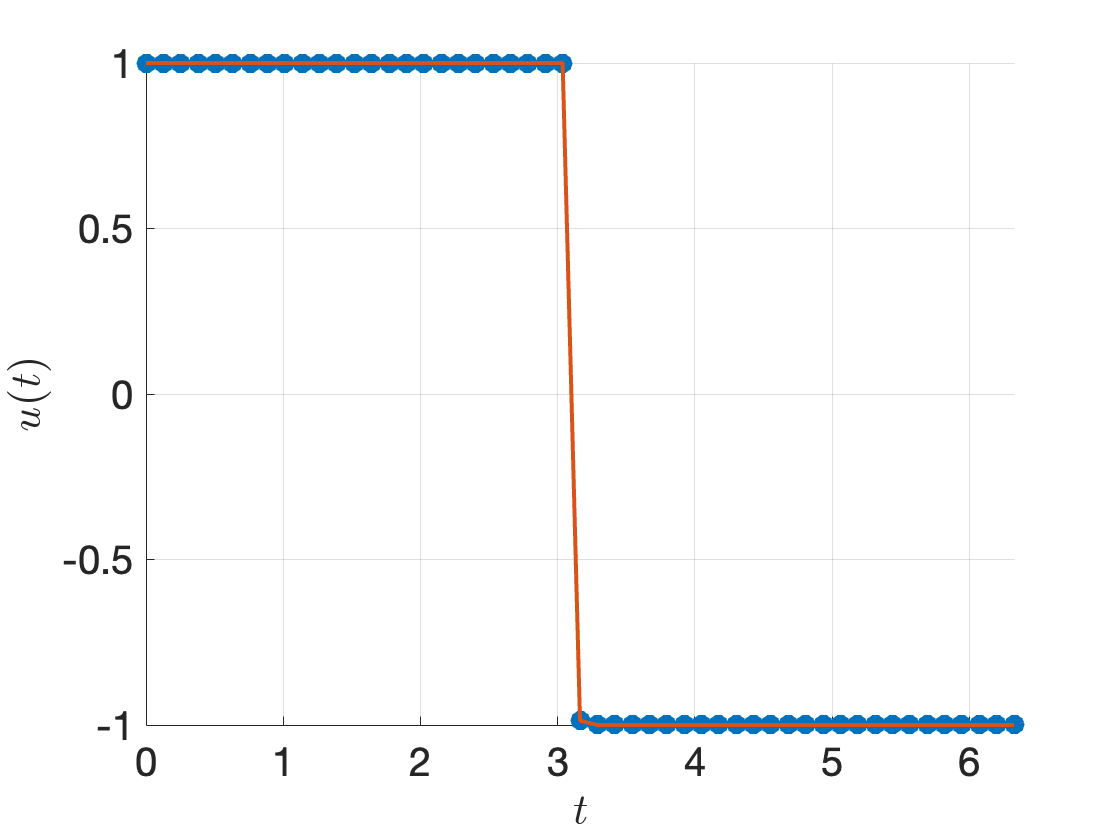
\includegraphics[width=0.7\linewidth]{images/min_time_di_u} 

}

\caption{Optimal control signal by direct multiple shooting.}\label{fig:min-time-di-u-ms}
\end{figure}

Using \texttt{ode45} to integrate the double integrator dynamics from \(x_0\) with the controller in Fig. \ref{fig:min-time-di-u-ms}, we obtain the following state trajectory. Notice that the final state does not exactly land at the origin. This is expected due to our time discretization and imperfect dynamics integration using \texttt{ode45}. Make sure you play with the code, e.g., by changing the initial state \(x_0\) and see what happens.

\begin{figure}

{\centering 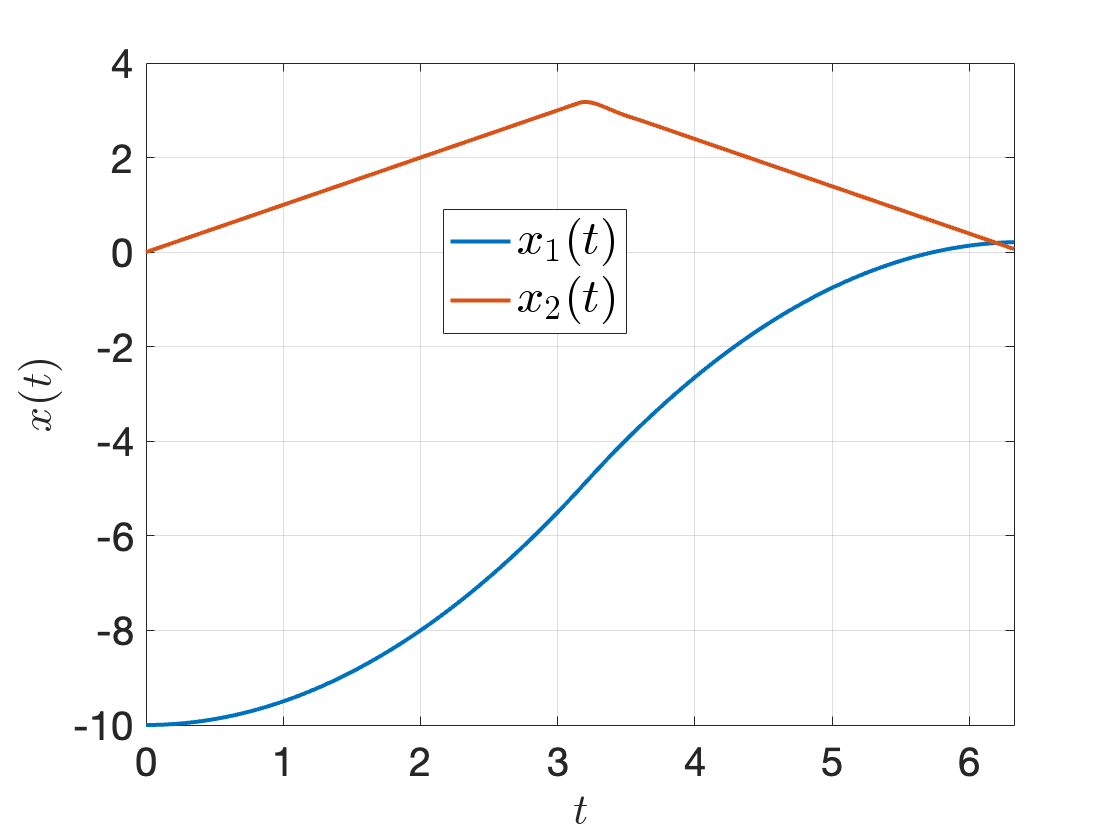
\includegraphics[width=0.7\linewidth]{images/min_time_di_x} 

}

\caption{ODE45 integration with the optimal control signal found by direct multiple shooting.}\label{fig:min-time-di-x-ms}
\end{figure}

\end{example}

\hypertarget{direct-collocation}{%
\subsection{Direct Collocation}\label{direct-collocation}}

In direct multiple shooting, we still need to rely on the numerical integrator RK4, which complicates the original nonlinear dynamics. In direct collocation, we will remove our dependency of RK4.

The key idea of direct collocation is to approximate the state trajectory \(x(t)\) and the control trajectory \(u(t)\) as piece-wise polynomial functions. In the following, we will describe the Hermite-Simpson collocation method.

\begin{figure}

{\centering 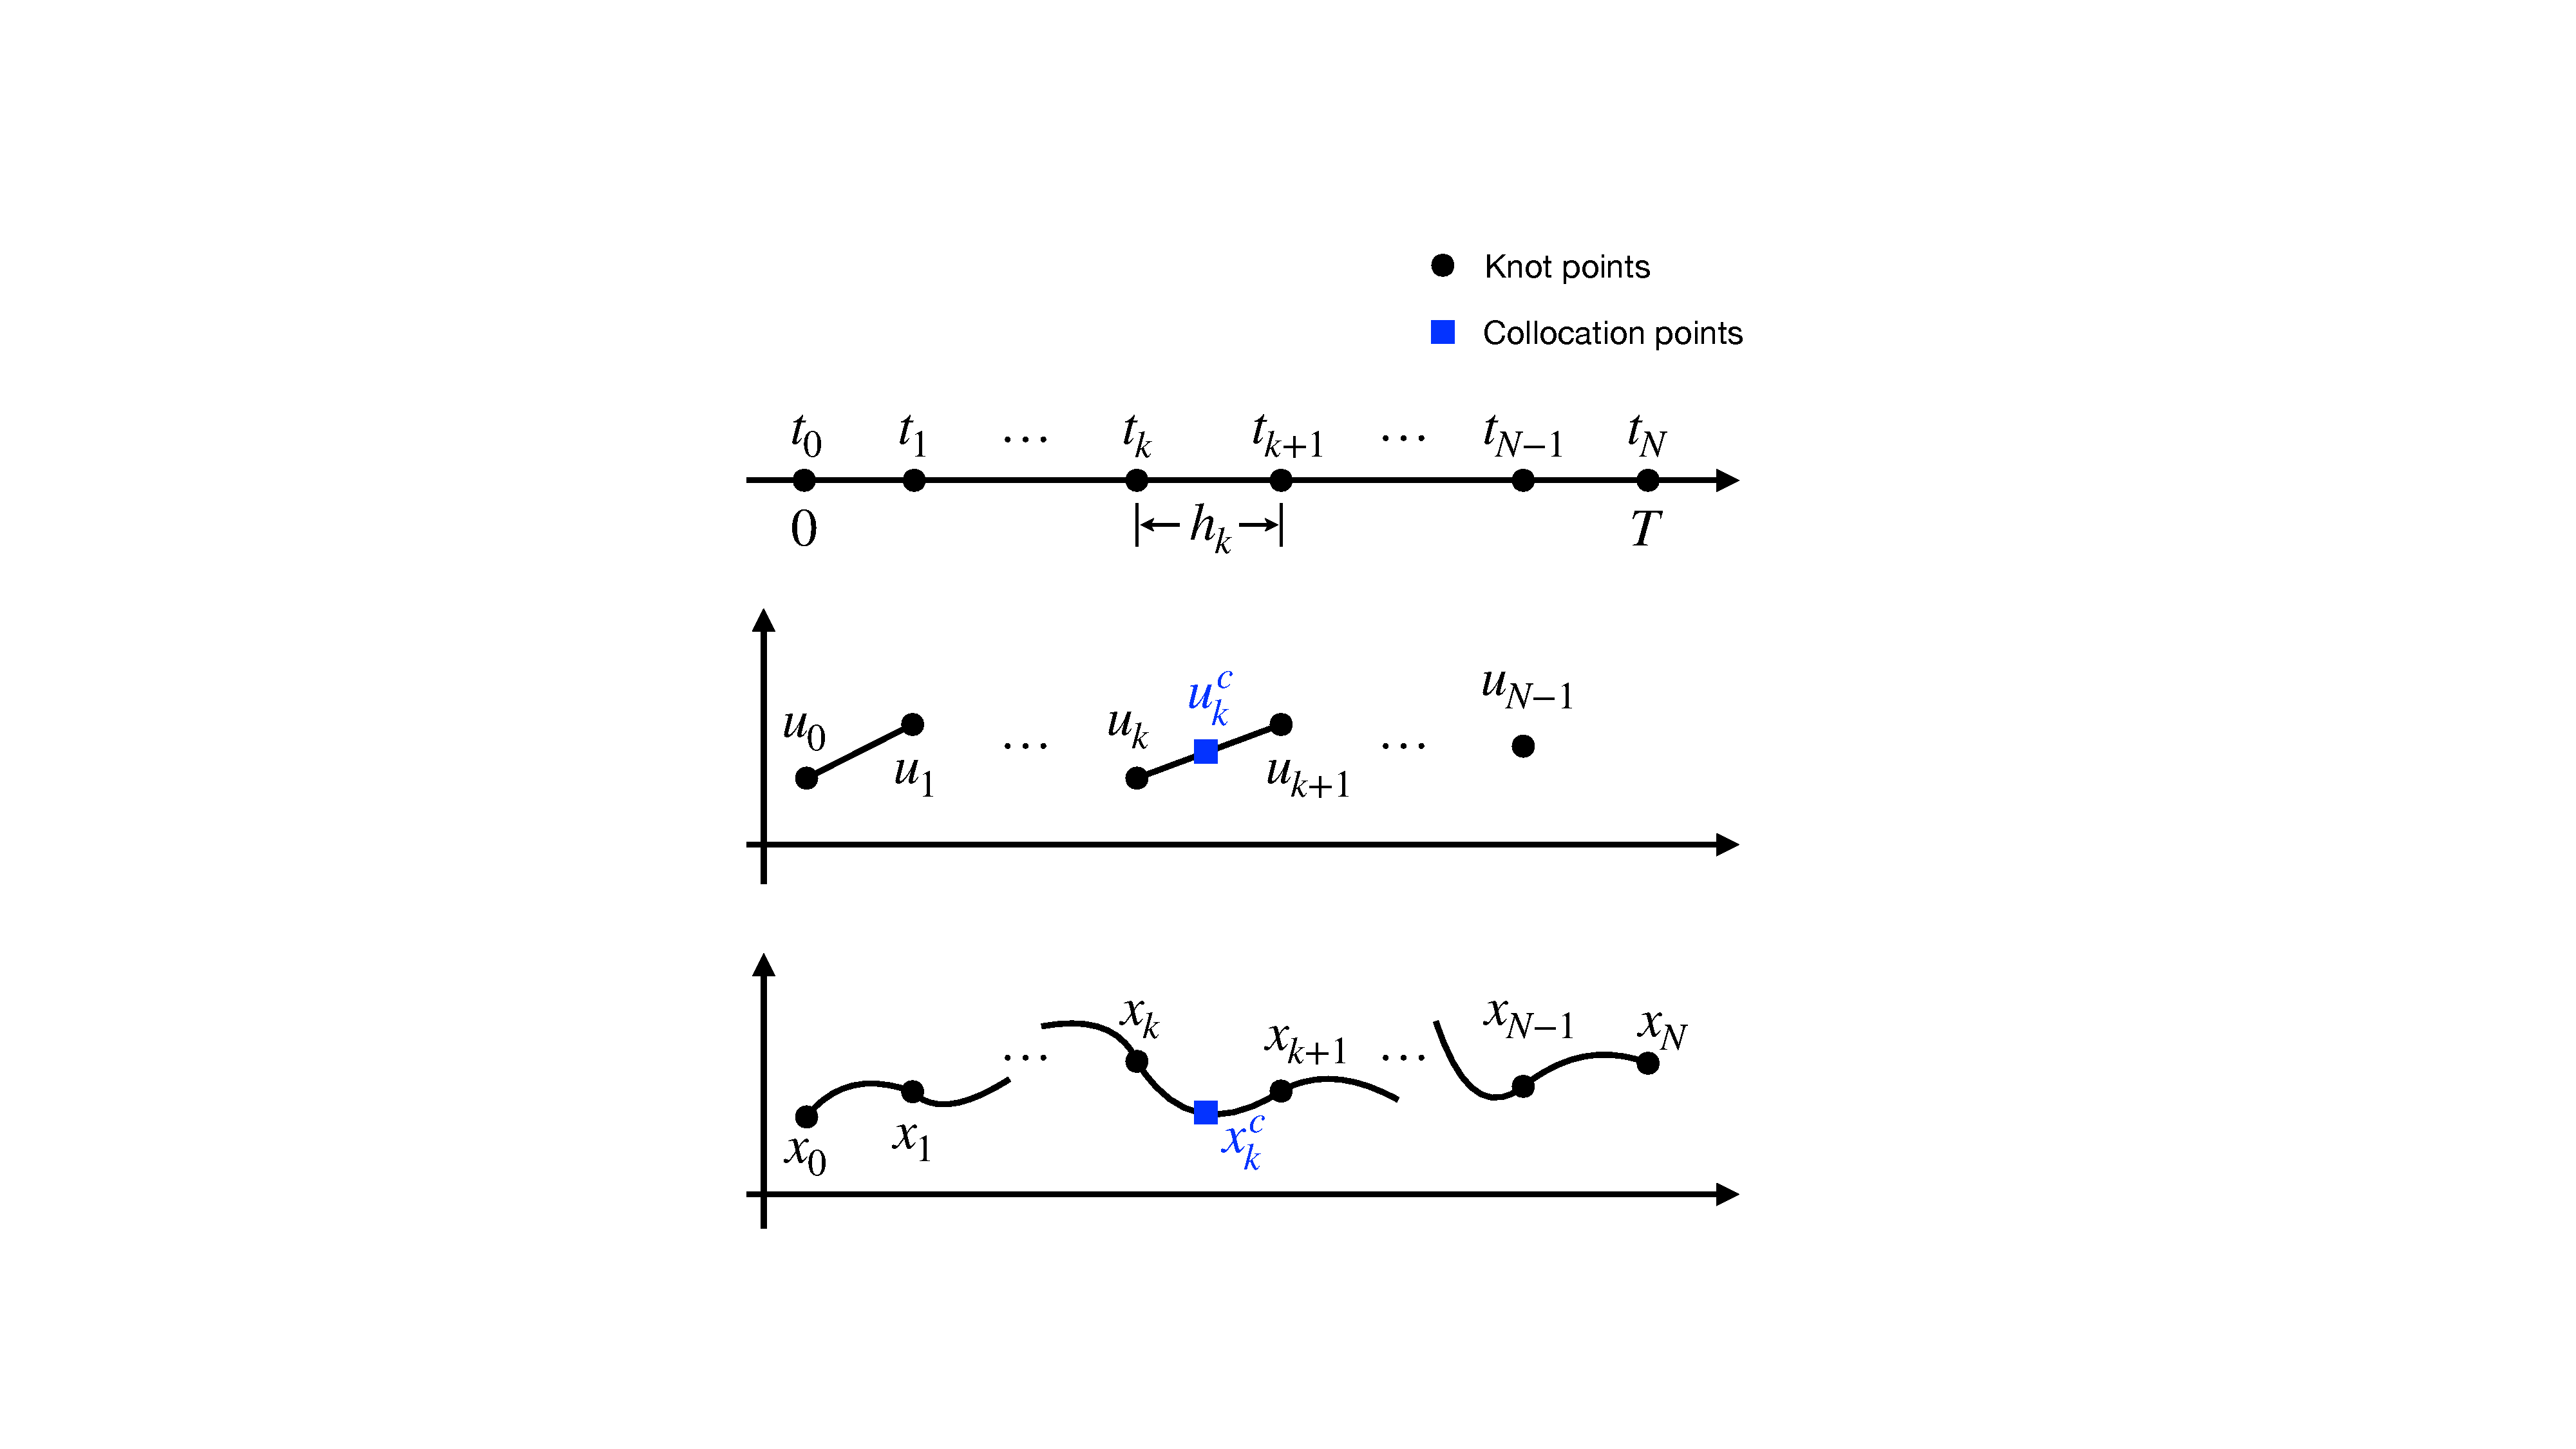
\includegraphics[width=0.6\linewidth]{images/direct_collocation} 

}

\caption{Direct collocation.}\label{fig:direct-collocation}
\end{figure}

\textbf{Time discretization}. We first discretize the total time window \([0,T]\) into a set of \(N\) intervals:
\[
0 = t_0 \leq t_1 \leq \dots \leq t_k \leq t_{k+1} \leq \dots \leq t_N = T.
\]
We denote
\[
h_k = t_{k+1} - t_k
\]
as the length of the \(k\)-th time interval. As we will see, the length of the time interval does not need to be fixed, and instead they can themselves be unknown variables to be optimized (in which case the final time \(T\) also becomes flexible).

\textbf{Knot variables}. At each of the timestamps \(t_0,\dots,t_N\), we assign \emph{knot variables}, which are unknown state and control varaibles that need to be optimized. In particular, we have state knot variables
\[
x_k = x(t_k), k=1,\dots,N,
\]
and control knot variables
\[
u_k = u(t_k),k=0,\dots,N-1.
\]
As a result, the entire set of knot varaibles to be optimized is
\begin{equation}
v = \begin{bmatrix} u_0 \\ u_1 \\ \vdots \\ u_{N-1} \\ x_1 \\ x_2 \\ \vdots \\ x_{N} \end{bmatrix}.
\label{eq:knot-variables}
\end{equation}
If the time-discretization is also optimized, then \(v\)
includes the time intervals as well.

\textbf{Transcribe dynamics}. The most important step is to transcribe the nonlinear dynamics \(\dot{x}=f(x(t),u(t))\) as constraints on the knot varaibles. In direct collocation, the way this is done is to enforce the dynamics equation at the set of \emph{collocation points} that are the mid-points between each consecutive pair of knot variables \((x_k, x_{k+1})\).

Specifically, in each subinterval \([t_k, t_{k+1}]\), we approximate the state trajectory as a cubic polynomial
\begin{equation}
x(t) = p_{k,0} + p_{k,1}(t-t_k) + p_{k,2}(t-t_k)^2 + p_{k,3}(t - t_k)^3, \quad t \in [t_k, t_{k+1}],
\label{eq:state-polynomial}
\end{equation}
where \(p_{k,0},p_{k,1},p_{k,2},p_{k,3} \in \mathbb{R}^n\) are the coefficients of the polynomial. You would think that we would need to optimize the coefficients as well, but actually we won't need to, as will be shown soon.
With this parameterization, we can obtain the time derivative of \(x(t)\) as
\begin{equation}
\dot{x}(t) = p_{k,1} + 2 p_{k,2}(t-t_k) + 3p_{k,3}(t - t_k)^2, \quad t \in [t_k, t_{k+1}].
\label{eq:state-polynomial-derivative}
\end{equation}
Now the key step is to write the coefficients \(p_{k,0},p_{k,1},p_{k,2},p_{k,3}\) using our knot variables \eqref{eq:knot-variables}. To do so, we can invoke \eqref{eq:state-polynomial} and \eqref{eq:state-polynomial-derivative} to obtain
\[
\begin{bmatrix}
x_k \\
\dot{x}_k = f(x_k,u_k) \\
x_{k+1} \\
\dot{x}_{k+1} = f(x_{k+1}, u_{k+1})
\end{bmatrix}
= \begin{bmatrix}
I & 0 & 0 & 0 \\
0 & I & 0 & 0 \\
I & h_k I & h_k^2 I & h_k^3 I \\
0 & I & 2 h_k I & 3 h_k^2 I \end{bmatrix}
\begin{bmatrix}
p_{k,0}\\
p_{k,1}\\
p_{k,2}\\
p_{k,3}
\end{bmatrix}.
\]
Solving the above equation, we get
\begin{equation}
\begin{bmatrix}
p_{k,0}\\
p_{k,1}\\
p_{k,2}\\
p_{k,3}
\end{bmatrix} = 
\begin{bmatrix}
I & 0 & 0 & 0 \\
0 & I & 0 & 0 \\
- \frac{3}{h_k^2} I & - \frac{2}{h_k} I & \frac{3}{h_k^2} I & -\frac{1}{h_k} I \\
\frac{2}{h_k^3} I & \frac{1}{h_k^2} I & -\frac{2}{h_k^3} I & \frac{1}{h_k^2} I 
\end{bmatrix}
\begin{bmatrix}
x_k \\
f(x_k,u_k) \\
x_{k+1} \\
f(x_{k+1}, u_{k+1})
\end{bmatrix}.
\label{eq:polynomial-coefficients-closed-form}
\end{equation}
Equation \eqref{eq:polynomial-coefficients-closed-form} implies, using the knot variables \(v\) in \eqref{eq:knot-variables}, we can query the value of \(x(t)\) and \(\dot{x}(t)\) at any time \(t \in [0,T]\). In particular, we will query the values of \(x(t)\) and \(\dot{x}(t)\) at the midpoints to obtain
\[
x_k^c = x\left( t_k + \frac{h_k}{2} \right) = \frac{1}{2} (x_k + x_{k+1}) + \frac{h_k}{8} (f(x_k,u_k) - f(x_{k+1},u_{k+1})),
\]
and
\[
\dot{x}_k^c = \dot{x} \left( t_k + \frac{h_k}{2} \right) = - \frac{3}{2h_k} (x_k - x_{k+1}) - \frac{1}{4} \left( f(x_k,u_k) + f(x_{k+1},u_{k+1}) \right).
\]
At the midpoint, we assume the control is
\[
u_k^c = \frac{1}{2}(u_k + u_{k+1}).
\]
Therefore, we can enforce the dynamics constraint at the midpoint as
\begin{equation}
\dot{x}^c_k = f(x_k^c, u_k^c).
\label{eq:collocation-constraint}
\end{equation}

\textbf{Transcribe other constraints}. The other constraints in the continuous-time formulation \eqref{eq:constrained-optimal-control} can be transcribed to the knot variables in a straightforward way:
\begin{align}
x_k \in \mathcal{X} \Rightarrow c_i^x(x_k)\geq 0, i=1,\dots,q_x, \quad k=1,\dots,N \\
u_k \in \mathcal{X} \Rightarrow c^u_i(u_k) \geq 0, i=1,\dots,q_u, \quad k=0,\dots,N-1\\
\phi_i(x_k, u_k) \geq 0, i=1,\dots,q, \quad k=0,\dots,N.
\end{align}

\textbf{Transcribe the objective}. We can write the objective as
\[
g_T(x_N) + \sum_{k=0}^{N-1} \frac{g(x_k,u_k) + g(x_{k+1},u_{k+1})}{2} h_k.
\]

\textbf{Summary}. In summary, the final optimization problem becomes

\begin{equation} 
\begin{split}
\min_{u_0,\dots,u_{N-1},x_1,\dots,x_N} & \quad  g_T(x_N) + \sum_{k=0}^{N-1} \frac{g(x_k,u_k) + g(x_{k+1},u_{k+1})}{2} h_k \\
\text{subject to} & \quad \dot{x}_k^c = f(x_k^c,u_k^c), \quad k=0,\dots,N-1 \\
& \quad c_i^x(x_k) \geq 0,i=1,\dots,q_x, \quad k=1,\dots,N \\
& \quad c_i^u(u_k) \geq 0,i=1,\dots,q_u, \quad k=0,\dots,N-1 \\
& \quad \phi_i (x_k,u_k) \geq 0, i=1,\dots,q, \quad k=0,\dots,N.
\end{split}
\label{eq:constrained-optimal-control-nlp}
\end{equation}

Let us apply direct collocation to the same double integrator Example \ref{exm:multiple-shooting-double-integrator}.

\begin{example}[Direct Collocation for Minimum-Time Double Integrator]
\protect\hypertarget{exm:collocation-double-integrator}{}\label{exm:collocation-double-integrator}

Consider the same minimum-time optimal control problem in Example \ref{exm:multiple-shooting-double-integrator}.

To apply direct collocation, we have our NLP variable
\[
v = (T,x_0,\dots,x_N,u_0,\dots,u_N).
\]
Similarly we can enforce the control constraints and the initial / terminal constraints.

The following script shows how to enforce the collocation constraint.

\begin{Shaded}
\begin{Highlighting}[]
\KeywordTok{function}\NormalTok{ [}\VariableTok{c}\OperatorTok{,}\VariableTok{ceq}\NormalTok{] }\OperatorTok{=} \VariableTok{collocation}\NormalTok{(}\VariableTok{v}\OperatorTok{,}\VariableTok{N}\OperatorTok{,}\VariableTok{initial\_state}\NormalTok{)}
\VariableTok{T} \OperatorTok{=} \VariableTok{v}\NormalTok{(}\FloatTok{1}\NormalTok{)}\OperatorTok{;}
\VariableTok{h} \OperatorTok{=} \VariableTok{T}\OperatorTok{/}\NormalTok{(}\VariableTok{N}\OperatorTok{{-}}\FloatTok{1}\NormalTok{)}\OperatorTok{;}
\VariableTok{x} \OperatorTok{=} \VariableTok{reshape}\NormalTok{(}\VariableTok{v}\NormalTok{(}\FloatTok{2}\OperatorTok{:}\FloatTok{2}\OperatorTok{*}\VariableTok{N}\OperatorTok{+}\FloatTok{1}\NormalTok{)}\OperatorTok{,}\FloatTok{2}\OperatorTok{,}\VariableTok{N}\NormalTok{)}\OperatorTok{;}
\VariableTok{u} \OperatorTok{=} \VariableTok{v}\NormalTok{(}\FloatTok{2}\OperatorTok{*}\VariableTok{N}\OperatorTok{+}\FloatTok{2}\OperatorTok{:}\KeywordTok{end}\NormalTok{)}\OperatorTok{;}
\VariableTok{c} \OperatorTok{=}\NormalTok{ []}\OperatorTok{;}
\VariableTok{ceq} \OperatorTok{=}\NormalTok{ []}\OperatorTok{;}
\KeywordTok{for} \VariableTok{k}\OperatorTok{=}\FloatTok{1}\OperatorTok{:}\VariableTok{N}\OperatorTok{{-}}\FloatTok{1}
    \VariableTok{uk} \OperatorTok{=} \VariableTok{u}\NormalTok{(}\VariableTok{k}\NormalTok{)}\OperatorTok{;}
    \VariableTok{ukp1} \OperatorTok{=} \VariableTok{u}\NormalTok{(}\VariableTok{k}\OperatorTok{+}\FloatTok{1}\NormalTok{)}\OperatorTok{;}
    \VariableTok{xk} \OperatorTok{=} \VariableTok{x}\NormalTok{(}\OperatorTok{:,}\VariableTok{k}\NormalTok{)}\OperatorTok{;}
    \VariableTok{xkp1} \OperatorTok{=} \VariableTok{x}\NormalTok{(}\OperatorTok{:,}\VariableTok{k}\OperatorTok{+}\FloatTok{1}\NormalTok{)}\OperatorTok{;}
    \VariableTok{fk} \OperatorTok{=} \VariableTok{double\_integrator}\NormalTok{(}\VariableTok{xk}\OperatorTok{,}\VariableTok{uk}\NormalTok{)}\OperatorTok{;}
    \VariableTok{fkp1} \OperatorTok{=} \VariableTok{double\_integrator}\NormalTok{(}\VariableTok{xkp1}\OperatorTok{,}\VariableTok{ukp1}\NormalTok{)}\OperatorTok{;}
    \CommentTok{\% collocation points}
    \VariableTok{xkc} \OperatorTok{=} \FloatTok{0.5}\OperatorTok{*}\NormalTok{(}\VariableTok{xk}\OperatorTok{+}\VariableTok{xkp1}\NormalTok{) }\OperatorTok{+} \VariableTok{h}\OperatorTok{/}\FloatTok{8} \OperatorTok{*}\NormalTok{ (}\VariableTok{fk} \OperatorTok{{-}} \VariableTok{fkp1}\NormalTok{)}\OperatorTok{;}
    \VariableTok{ukc} \OperatorTok{=} \FloatTok{0.5}\OperatorTok{*}\NormalTok{(}\VariableTok{uk} \OperatorTok{+} \VariableTok{ukp1}\NormalTok{)}\OperatorTok{;}
    \VariableTok{dxkc} \OperatorTok{=} \OperatorTok{{-}}\FloatTok{3}\OperatorTok{/}\NormalTok{(}\FloatTok{2}\OperatorTok{*}\VariableTok{h}\NormalTok{) }\OperatorTok{*}\NormalTok{ (}\VariableTok{xk}\OperatorTok{{-}}\VariableTok{xkp1}\NormalTok{) }\OperatorTok{{-}} \FloatTok{0.25}\OperatorTok{*}\NormalTok{(}\VariableTok{fk} \OperatorTok{+} \VariableTok{fkp1}\NormalTok{)}\OperatorTok{;}
    \CommentTok{\% collocation constraint}
    \VariableTok{ceq} \OperatorTok{=}\NormalTok{ [}\VariableTok{ceq}\OperatorTok{;}
           \VariableTok{dxkc} \OperatorTok{{-}} \VariableTok{double\_integrator}\NormalTok{(}\VariableTok{xkc}\OperatorTok{,}\VariableTok{ukc}\NormalTok{)]}\OperatorTok{;}
\KeywordTok{end}
\VariableTok{ceq} \OperatorTok{=}\NormalTok{ [}\VariableTok{ceq}\OperatorTok{;}
       \VariableTok{x}\NormalTok{(}\OperatorTok{:,}\FloatTok{1}\NormalTok{) }\OperatorTok{{-}} \VariableTok{initial\_state}\OperatorTok{;} \CommentTok{\% initial condition}
       \VariableTok{x}\NormalTok{(}\OperatorTok{:,}\KeywordTok{end}\NormalTok{)]}\OperatorTok{;} \CommentTok{\% land at zero}
\KeywordTok{end}
\end{Highlighting}
\end{Shaded}

As you can see, we do not need any numerical integrator such as \texttt{ode45}. The only thing we need is the continuous-time double integrator dynamics.

Running the \href{https://github.com/ComputationalRobotics/OptimalControlEstimation-Examples/blob/main/double_integrator_collocation.m}{complete code} with \(x_0 = (-10,0)\) and \(N=51\), we get the control signal in Fig. \ref{fig:min-time-di-u-collocation} that is bang-bang.

\begin{figure}

{\centering 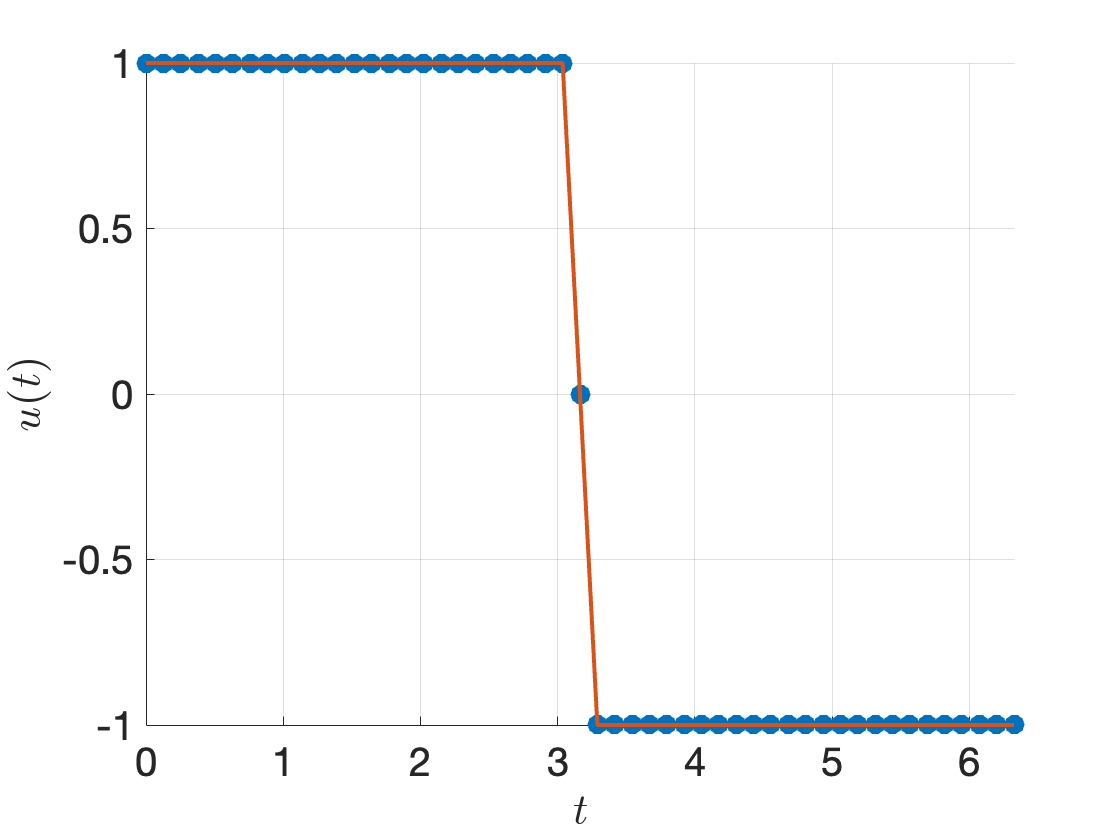
\includegraphics[width=0.7\linewidth]{images/min_time_di_u_collocation} 

}

\caption{Optimal control signal by direct collocation.}\label{fig:min-time-di-u-collocation}
\end{figure}

Using \texttt{ode45} to integrate the double integrator dynamics from \(x_0\) with the controller in Fig. \ref{fig:min-time-di-u-collocation}, we obtain the following state trajectory. Comparing Fig. \ref{fig:min-time-di-x-collocation} with Fig. \ref{fig:min-time-di-x-ms}, we can observe that the terminal state of the trajectory obtained from direct collocation is more accurate than that obtained from direct multiple shooting.

\begin{figure}

{\centering 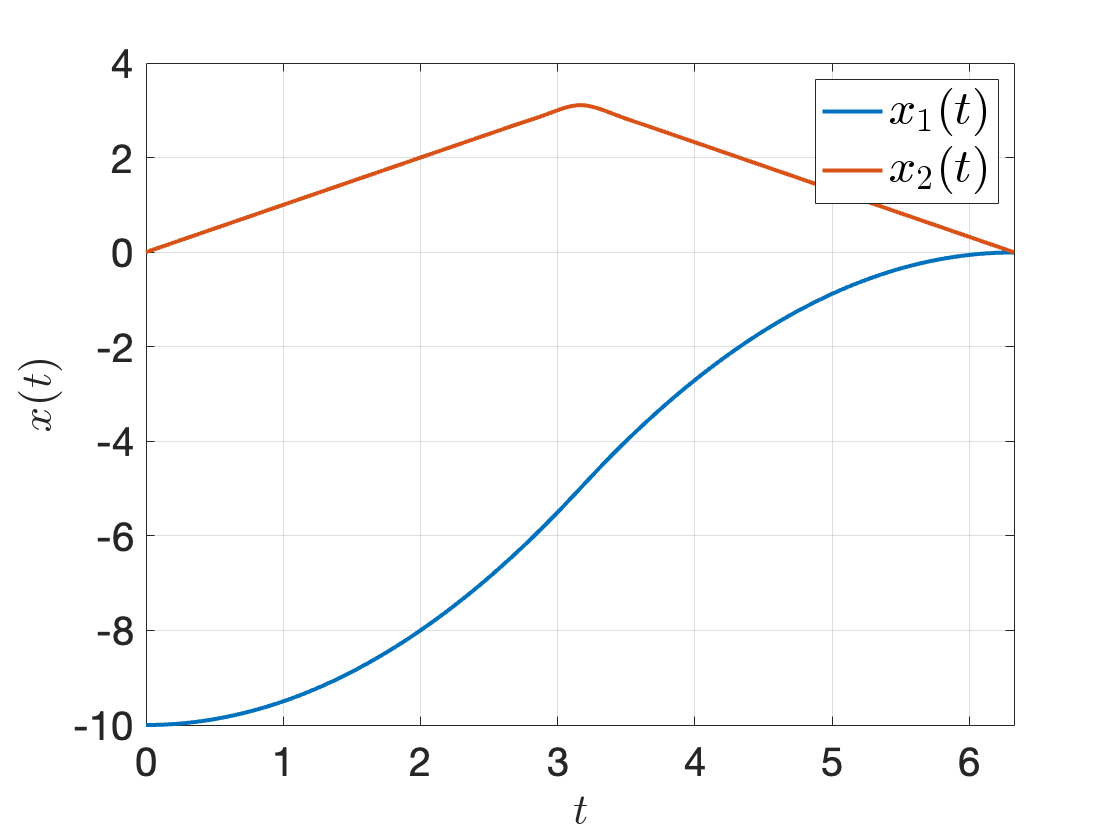
\includegraphics[width=0.7\linewidth]{images/min_time_di_x_collocation} 

}

\caption{ODE45 integration with the optimal control signal found by direct collocation.}\label{fig:min-time-di-x-collocation}
\end{figure}

Not only is direct collocation more accurate for this example, it is also faster. This is evident because in direct multiple shooting, evaluating the nonlinear constraints requires runing \texttt{ode45}, while in direct collocation, evaluating the nonlinear constraints simply requires calling the original continuous-time dynamics.

We can easily optimize with a larger \(N=101\) and get the following results.

\begin{figure}

{\centering 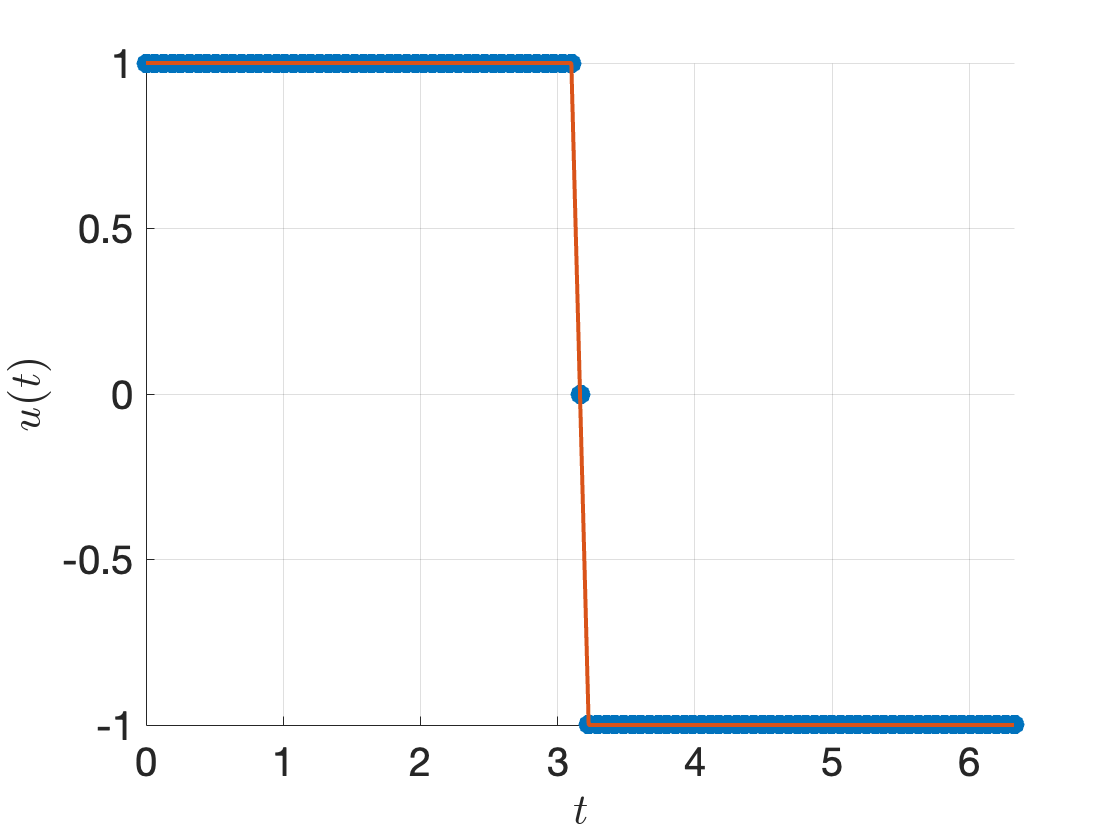
\includegraphics[width=0.45\linewidth]{images/min_time_di_u_collocation_N_100} 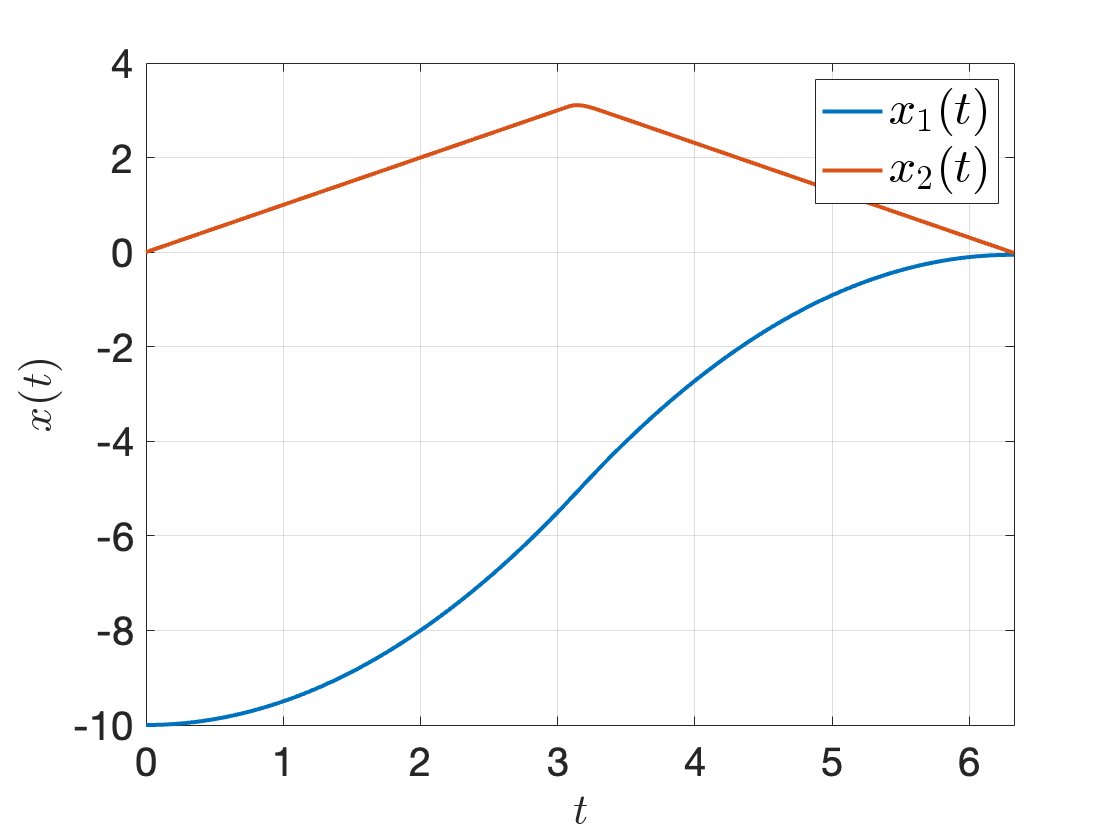
\includegraphics[width=0.45\linewidth]{images/min_time_di_x_collocation_N_100} 

}

\caption{Direct collocation with N=101.}\label{fig:min-time-di-u-x-collocation-N-100}
\end{figure}

\end{example}

If you are interested in direct collocation, there is a nice tutorial with Matlab examples in \citep{kelly17siam-trajopt}.

\hypertarget{direct-orthogonal-collocation}{%
\subsection{Direct Orthogonal Collocation}\label{direct-orthogonal-collocation}}

\hypertarget{failure-of-open-loop-control}{%
\subsection{Failure of Open-Loop Control}\label{failure-of-open-loop-control}}

Trajectory optimization produces very satisfying trajectories when the nonlinear programming algorithms work as expected, as shown by the previous Examples \ref{exm:collocation-double-integrator} and \ref{exm:multiple-shooting-double-integrator} on the double integrator system.

However, does this imply that if we simply run the planned controls on a real system, i.e., doing \emph{open-loop control}, the trajectory will behave as planned?

Unfortunately the answer is No, for two major reasons.

\begin{enumerate}
\def\labelenumi{\arabic{enumi}.}
\item
  Trajectory optimization only produces an \emph{approximate} solution to the optimal control problem (OCP) \eqref{eq:constrained-optimal-control}, regardless of what transcription method is used (such as multiple shooting and direct collocation). This means every \(u_k\) we obtained is an approximation to the true optimal controller \(u(t_k)\), and the approximation errors will accumulate as the dynamical system is evolving.
\item
  Even the OCP \eqref{eq:constrained-optimal-control} is an imperfect approximation of the true control task. This is due to we assumed we have perfect knowledge of the system dynamics
  \[
  \dot{x} = f(x(t),u(t)),
  \]
  which rarely holds in practice. For example, in the double integrator example, there is always friction between the mass and the ground. A more realistic assumption is that the system dynamics is
  \[
  \dot{x} = f(x(t),u(t)) + w_t,
  \]
  where \(w_t\) is some unknown disturbance, or modeling error.
\end{enumerate}

Let us observe the failure of open-loop control on our favorite pendulum example.

\begin{example}[Failure of Open-Loop Control on A Simple Pendulum]
\protect\hypertarget{exm:pendulum-collocation-failure}{}\label{exm:pendulum-collocation-failure}Consider an ``ideal'' pendulum dynamics model
\[
x = \begin{bmatrix} \theta \\ \dot{\theta} \end{bmatrix}, \quad \dot{x} = f(x,u) = \begin{bmatrix} \dot{\theta} \\ - \frac{1}{ml^2} (b \dot{\theta} + mgl \sin \theta) + \frac{1}{ml^2} u \end{bmatrix},
\]
with \(m=1,l=1,g=9.8,b=0.1\). We enforce control saturation
\[
u \in [-u_{\max}, u_{\max}]
\]
with \(u_{\max} = 4.9\).

\begin{figure}

{\centering 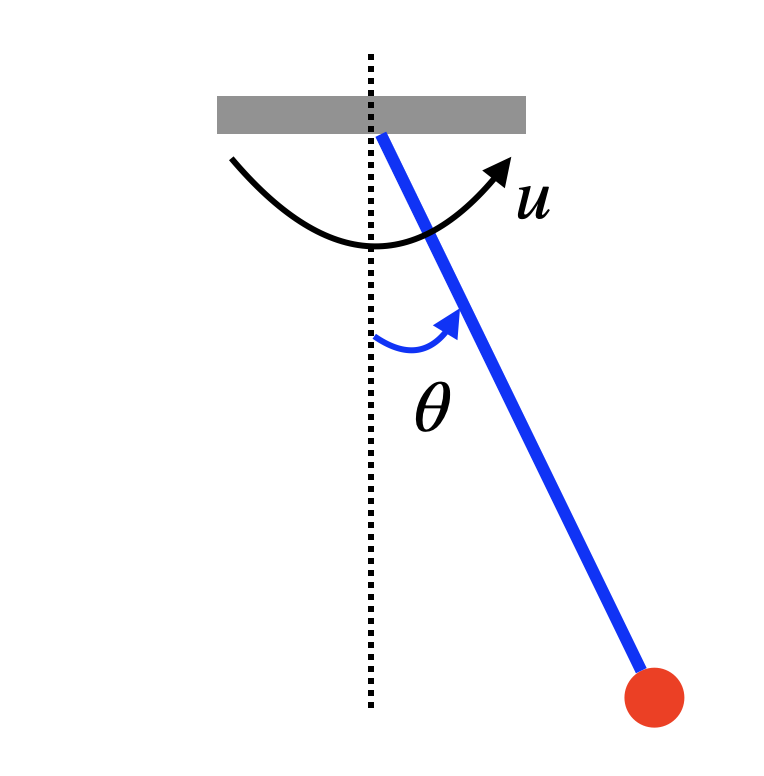
\includegraphics[width=0.4\linewidth]{images/pendulum-drawing} 

}

\caption{Simple pendulum.}\label{fig:pendulum-model-failure}
\end{figure}

Consider the optimal control problem with \(T=10\)
\begin{equation}
\begin{split} \min_{u(t), t \in [0,T]} & \quad \int_{t=0}^T (\cos \theta(t) + 1)^2 + \sin^2\theta(t) + \dot{\theta}^2(t) + u^2 dt \\
\text{subject to} & \quad \dot{x} = f(x(t),u(t)) \\
& \quad x(0) = [0,0]^T, \quad x(T) = [\pi,0]^T, \\
& \quad u(t) \in [-u_{\max},u_{\max}],
\end{split}
\label{eq:pendulum-swingup-ocp}
\end{equation}
where we start from the initial state \([0,0]^T\), i.e., the bottomright position, and we want to swing up the pendulum to the final state \([\pi,0]^T\), i.e., the upright position. The cost function in \eqref{eq:pendulum-swingup-ocp} penalizes the deviation of the state trajectory from the target state (the target state has \(\cos \theta = -1\), \(\sin \theta = 0\) and \(\dot{\theta} = 0\)), together with the magnitude of control.

\textbf{Trajectory optimization with direct collocation}. We perform trajectory optimization for the OCP \eqref{eq:pendulum-swingup-ocp} with direct collocation. We choose \(N=101\) break points with \(h=0.1\) equal interval to discretize the time.

The result of trajectory optimization is shown in Fig. \ref{fig:pendulum-swingup-trajopt-collocation}. We can see that the pendulum is perfectly swung up to \([\pi,0]^T\) and stabilized there.

\begin{figure}

{\centering 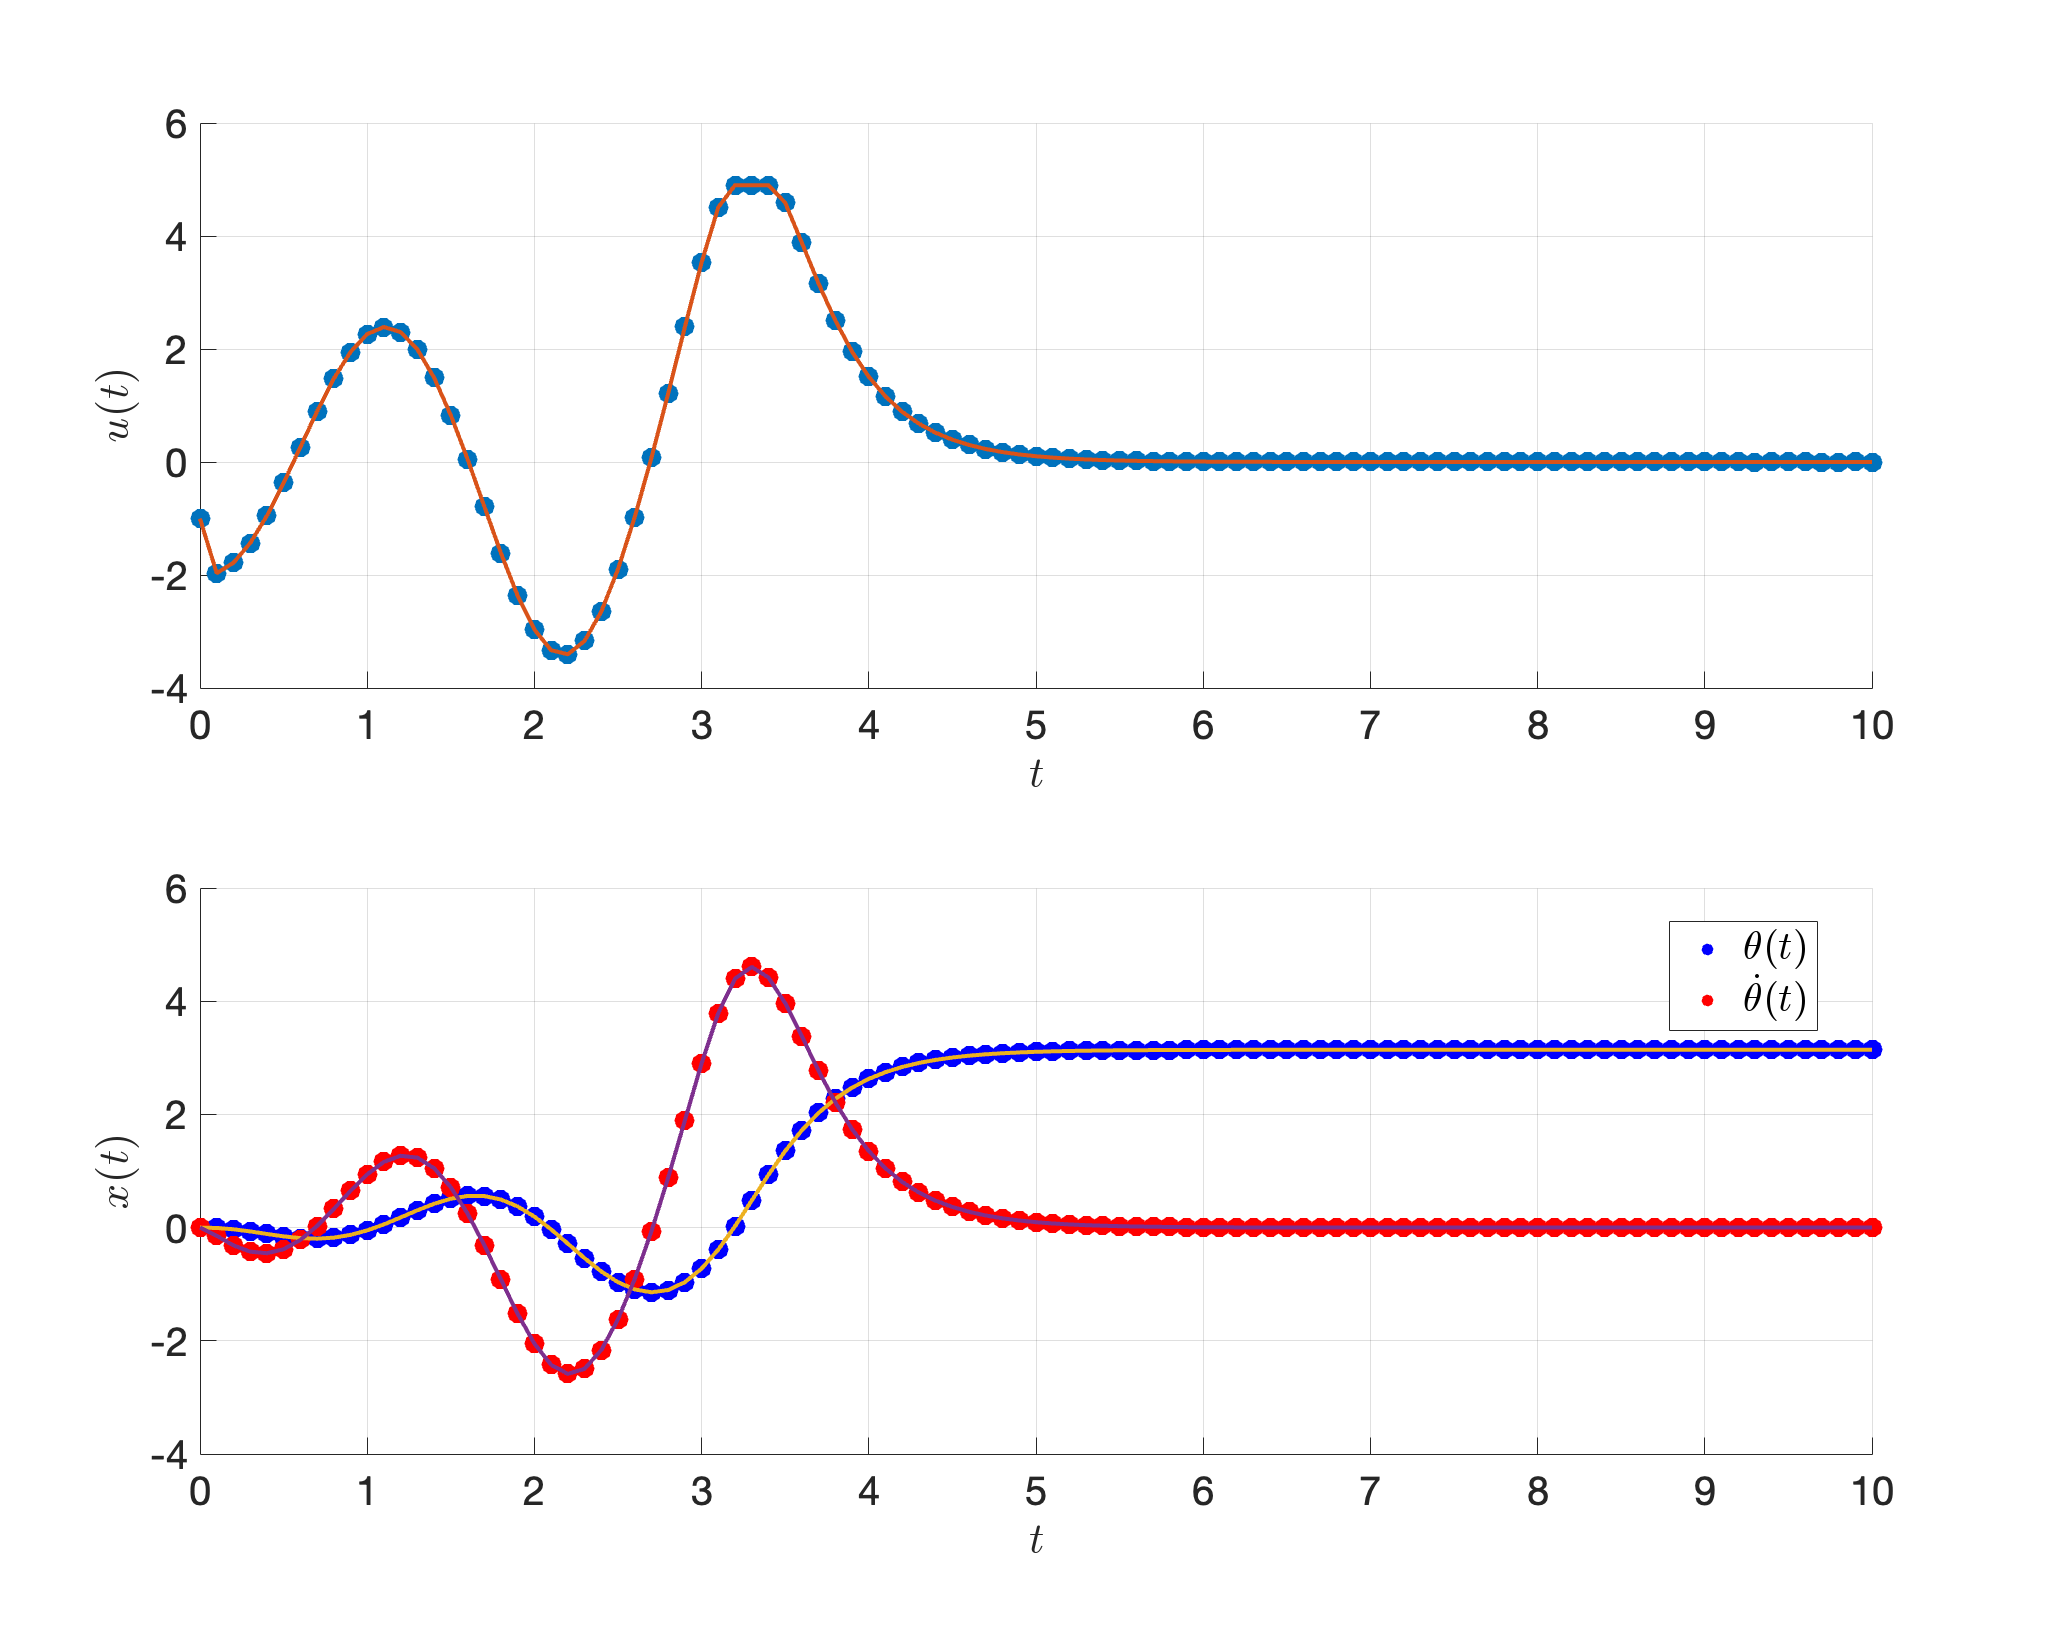
\includegraphics[width=0.8\linewidth]{images/pendulum_trajopt_result} 

}

\caption{Pendulum swing-up with direct collocation}\label{fig:pendulum-swingup-trajopt-collocation}
\end{figure}

\textbf{Deploy the optimized plan}. We then deploy the optimized controls in Fig. \ref{fig:pendulum-swingup-trajopt-collocation} on the ``ideal'' pendulum. We deploy the control every \(0.1\) seconds with zero-order hold, and use Matlab \texttt{ode89} to integrate the pendulum dynamics.

Fig. \ref{fig:pendulum-swingup-trajopt-collocation-deploy} shows the true trajectory of the pendulum. Unfortunately, the pendulum swing-up and stabilization is unsuccessful.

\begin{figure}

{\centering 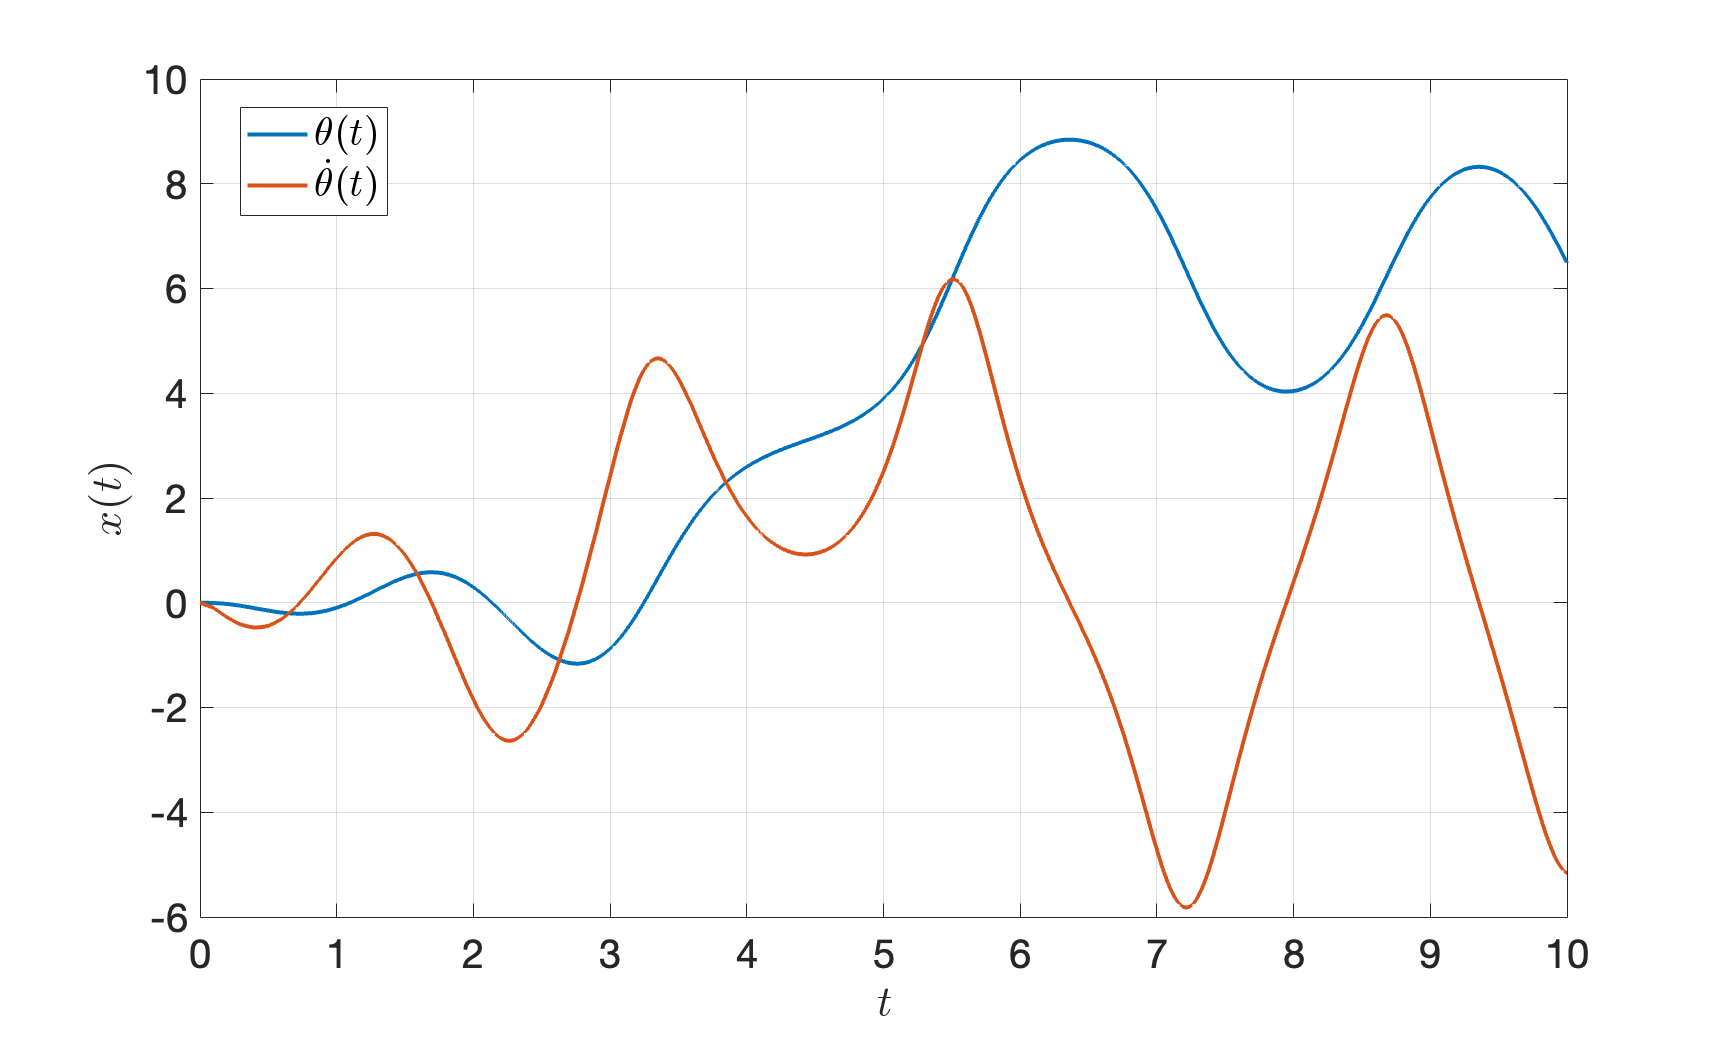
\includegraphics[width=0.8\linewidth]{images/pendulum_trajopt_deploy} 

}

\caption{Deploy optimized controls}\label{fig:pendulum-swingup-trajopt-collocation-deploy}
\end{figure}

\textbf{Adding noise}. What if the true pendulum dynamics is
\[
x = \begin{bmatrix} \theta \\ \dot{\theta} \end{bmatrix}, \quad \dot{x} = f(x,u) = \begin{bmatrix} \dot{\theta} \\ - \frac{1}{ml^2} (b \dot{\theta} + mgl \sin \theta) + \frac{1}{ml^2} u \end{bmatrix} + \begin{bmatrix} 0 \\ 1 \end{bmatrix}.
\]
That is, there is a constant unmodelled angular acceleration of \(1\), which maybe come from some unknown external force.

Fig. \ref{fig:pendulum-swingup-trajopt-collocation-deploy-noise} shows the trajectory of the pendulum with the optimized controlls. We can clearly see the unmodelled dynamics makes the performance much worse.

\begin{figure}

{\centering 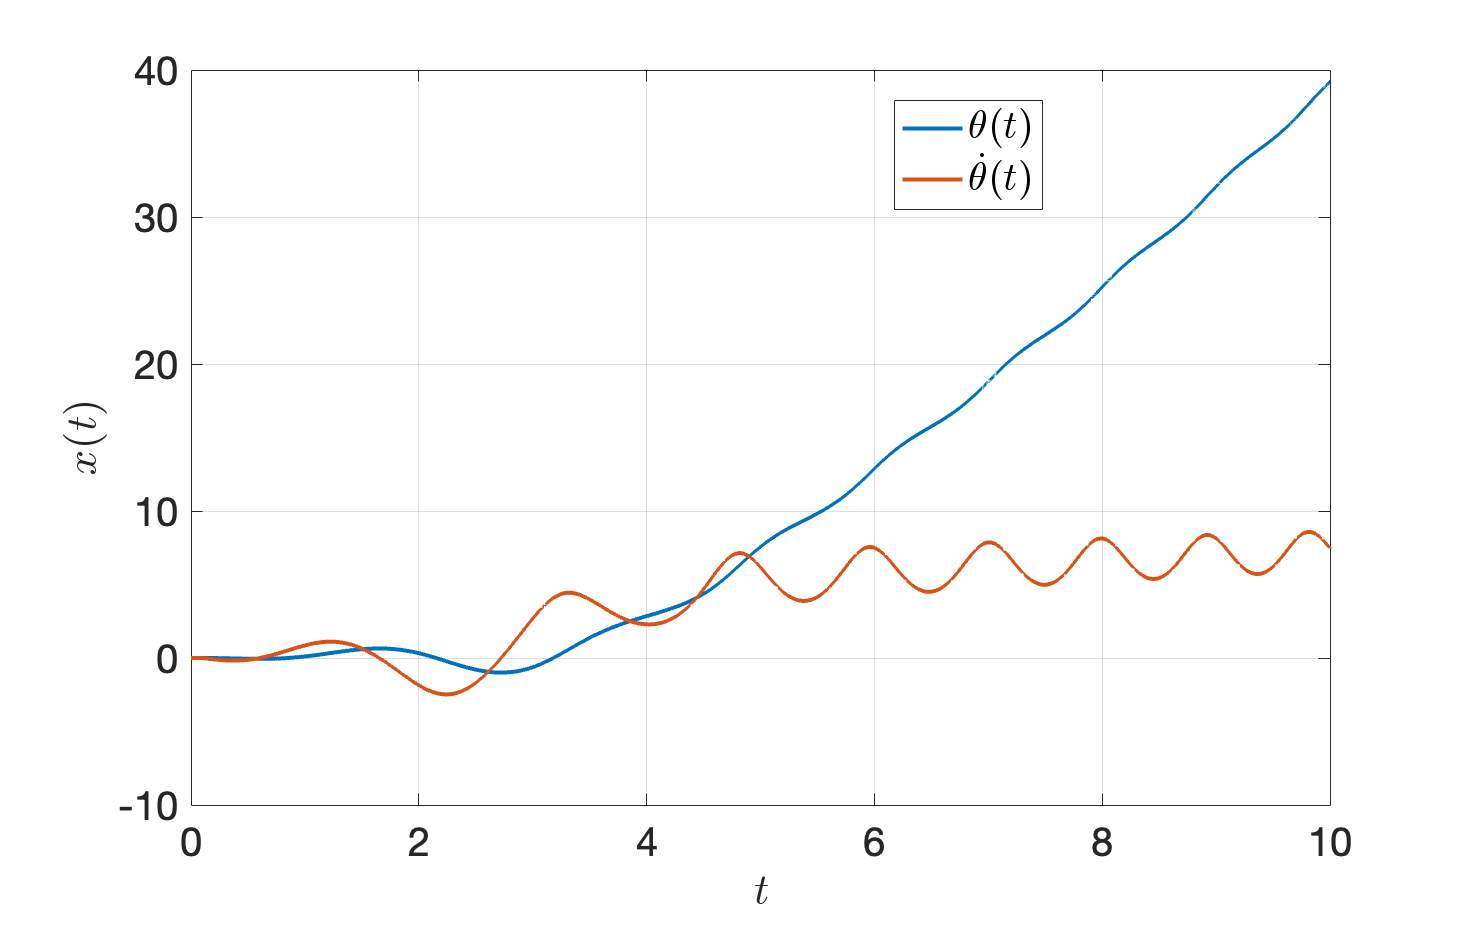
\includegraphics[width=0.8\linewidth]{images/pendulum_trajopt_deploy_noise} 

}

\caption{Deploy optimized controls on a system with disturbance}\label{fig:pendulum-swingup-trajopt-collocation-deploy-noise}
\end{figure}

You can play with the code \href{https://github.com/ComputationalRobotics/OptimalControlEstimation-Examples/blob/main/pendulum_mpc/pendulum_open_loop.m}{here}.
\end{example}

The failure of open-loop control motivates feedback control.

\hypertarget{lqr-trajectory-tracking}{%
\subsection{LQR Trajectory Tracking}\label{lqr-trajectory-tracking}}

\hypertarget{model-predictive-control}{%
\section{Model Predictive Control}\label{model-predictive-control}}

The model predictive control framework leverages the idea of \emph{receding horizon control} (RHC) to turn an open-loop controller into a closed-loop controller, i.e., a feedback controller.

For example, suppose we have an optimal control problem with horizon \(T\):
\begin{equation}
\begin{split}
\min_{u(t), t \in [0,T]} & \quad g_T(x(T)) + \int_{t=0}^T g(x(t),u(t)) dt \\
\text{subject to} & \quad \dot{x} = f(x(t),u(t)), \quad x(0) = x_0 \\
& (x(t),u(t)) \in \mathcal{X} \times \mathcal{U}, \quad x(T) \in \mathcal{X}_T 
\end{split}
\label{eq:optimal-control-problem-mpc}
\end{equation}
where \(\dot{x} = f(x(t),u(t))\) is the best ``ideal'' model we have about our system.

The idea of RHC is as follows. At time \(t\), we obtain a measurement of the current state of the system, denoted as \(x_t\), and we solve the following OCP with horizon \(H < T\):
\begin{equation}
\begin{split}
\min_{u(\tau), \tau \in [0,H]} & \quad g_t(x(H)) + \int_{\tau = 0}^H g(x(\tau),u(\tau)) d\tau \\
\text{subject to} & \quad  \dot{x} = f(x(\tau),u(\tau)), \quad x(0) = x_t \\
& \quad (x(t),u(t)) \in \mathcal{X} \times \mathcal{U}, \quad x(H) \in \mathcal{X}_{t}
\end{split}
\label{eq:optimal-control-problem-mpc-open-loop}
\end{equation}
where notice that I used a different notation for the terminal cost \(g_t\) (as supposed to \(g_T\) in \eqref{eq:optimal-control-problem-mpc}), and the terminal constraint \(\mathcal{X}_t\) (as supposed to \(\mathcal{X}_T\) in \eqref{eq:optimal-control-problem-mpc-open-loop}). Using a different terminal cost and terminal constraint is meant to make the problem \eqref{eq:optimal-control-problem-mpc-open-loop} always feasible.

Suppose we solve the open-loop control problem \eqref{eq:optimal-control-problem-mpc-open-loop} using trajectory optimization with \(N\) time intervals and obtained the following solution
\[
u_{t,0},u_{t,1},\dots,u_{t,N}.
\]
Then RHS will only take the first control \(u_{t,0}\) and apply it to the system. Therefore, the closed-loop dynamics is effectively
\begin{equation}
\dot{x} = f(x(t),u_{t,0}),
\label{eq:receding-horizon-control}
\end{equation}
where \(u_{t,0}\) is the first control solution to the OCP \eqref{eq:optimal-control-problem-mpc-open-loop}.

\begin{figure}

{\centering 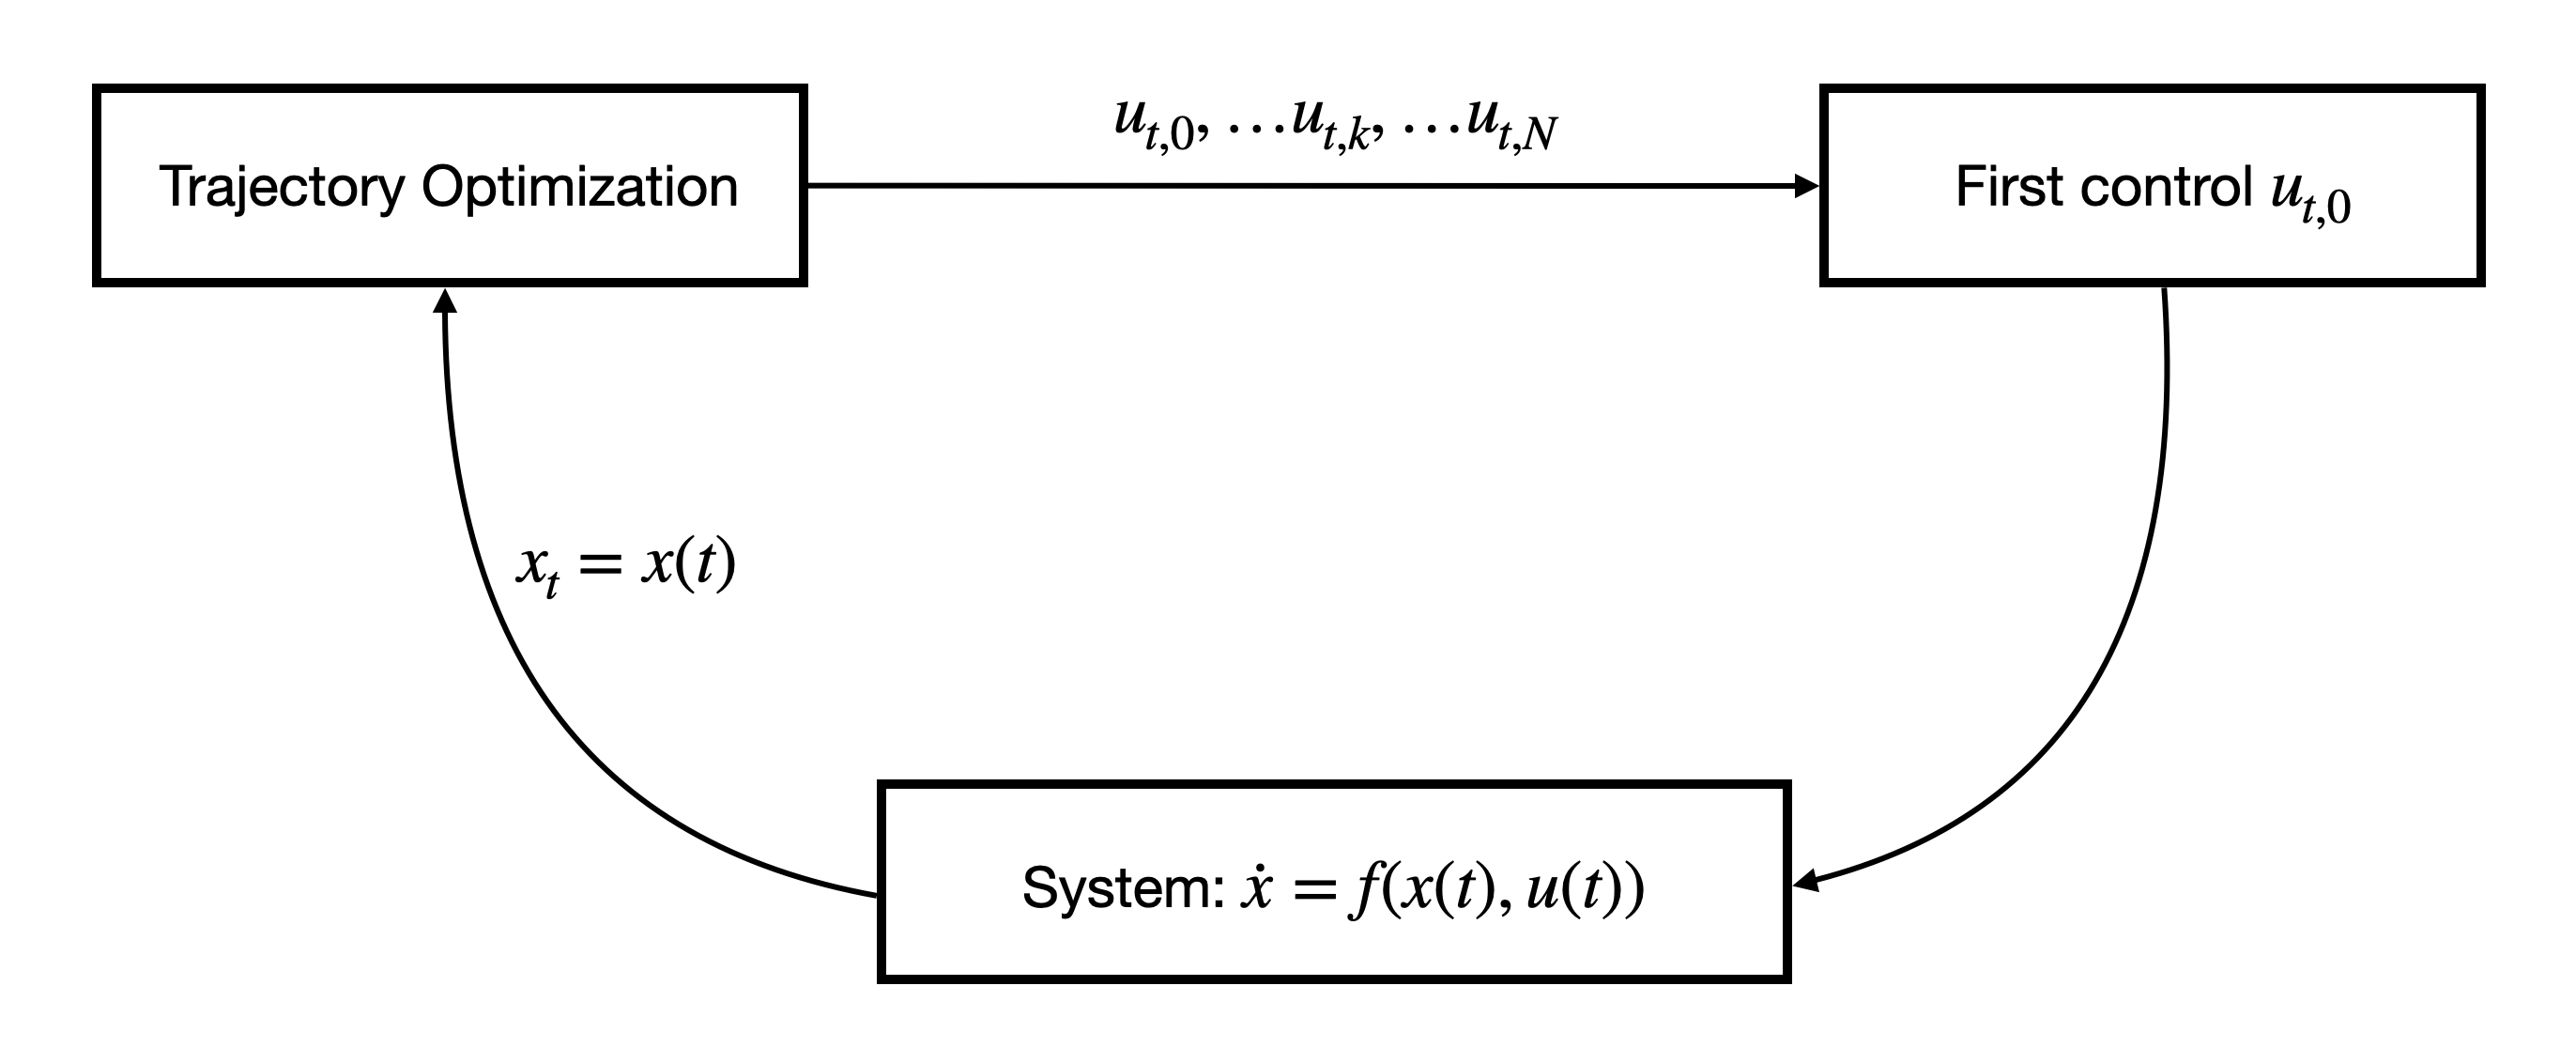
\includegraphics[width=0.8\linewidth]{images/receding_horizon_control} 

}

\caption{Receding horizon control}\label{fig:receding-horizon-control}
\end{figure}

It is worth noting that RHS effectively introduces feedback control, because the controller \(u_{t,0}\) in \eqref{eq:receding-horizon-control} depends on \(x(t)\) via the open-loop optimal control problem \eqref{eq:optimal-control-problem-mpc-open-loop}.

Trajectory optimization and model predictive control are the workhorse for control of highly dynamic robots. For example, here is a \href{https://youtu.be/EGABAx52GKI?feature=shared}{talk by Scott Kuindersma} on how trajectory optimization and model predictive control enable a diverse set of behaviors of Boston Dynamics's humanoid robot.

\hypertarget{turn-trajectory-optimization-into-feedback-control}{%
\subsection{Turn Trajectory Optimization into Feedback Control}\label{turn-trajectory-optimization-into-feedback-control}}

Let us turn our trajectory optimization algorithm in Example \ref{exm:pendulum-collocation-failure} into a feedback controller through receding horizon control.

\begin{example}[Pendulum Swingup with Model Predictive Control]
\protect\hypertarget{exm:mpc-pendulum-swingup}{}\label{exm:mpc-pendulum-swingup}Consider again the pendulum swingup task in Example \ref{exm:pendulum-collocation-failure}.

This time, we will apply MPC to this task.

Again, we discretize the time windown \([0,T]\) into \(N-1 = 100\) equal intervals with \(h = 0.1\). At each timestep \(t_k = kh\), \(k=0,\dots,N-1\), we first measure the current state of the pendulum as \(x_k\), then solve the following OCP with planning horizon \(H=5\)
\begin{equation}
\begin{split} \min_{u(t), t \in [0,H]} & \quad \int_{t=0}^H (\cos \theta(t) + 1)^2 + \sin^2\theta(t) + \dot{\theta}^2(t) + u^2 dt \\
\text{subject to} & \quad \dot{x} = f(x(t),u(t)) \\
& \quad x(0) = x_k, \quad x(H) = [\pi,0]^T, \\
& \quad u(t) \in [-u_{\max},u_{\max}].
\end{split}
\label{eq:pendulum-swingup-mpc-subroutine}
\end{equation}
We solve the OCP \eqref{eq:pendulum-swingup-mpc-subroutine} using trajectory optimization with direct collocation (using \(M\) break points), which gives us a sequence of controls
\[
u_{k,1},\dots,u_{k,M},
\]
we deploy the first control \(u_{k,1}\) to the pendulum system.

\textbf{MPC results}. Fig. \ref{fig:pendulum-swingup-mpc-noise-free} shows the control and state trajectories when using MPC to swing up the pendulum. We can see that it works very well.

\begin{figure}

{\centering 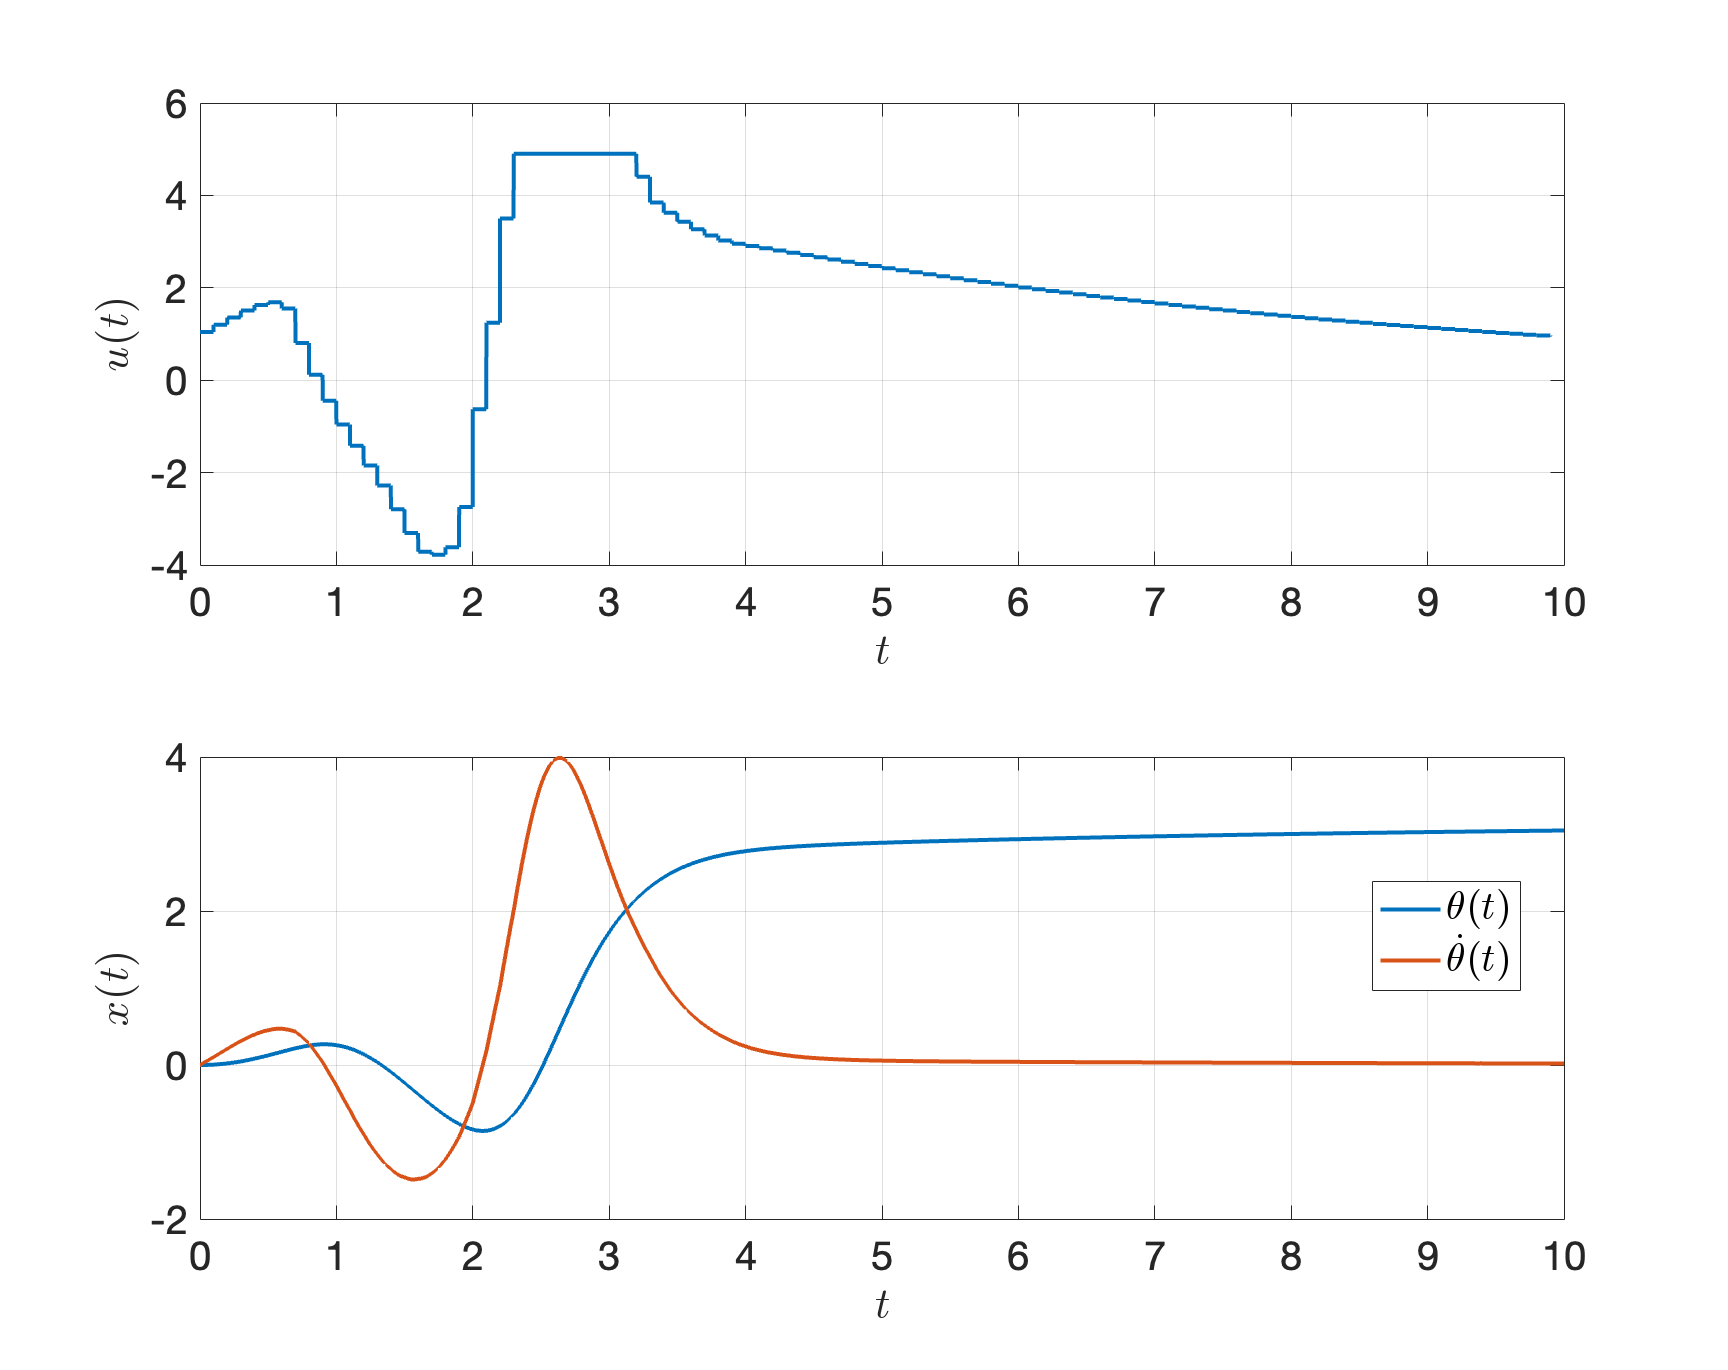
\includegraphics[width=0.8\linewidth]{images/pendulum_mpc_noise_free} 

}

\caption{MPC for pendulum swing-up}\label{fig:pendulum-swingup-mpc-noise-free}
\end{figure}

\textbf{Robustness to noise}. MPC is naturally robust to modelling errors and noises. When the true system dynamics is
\[
x = \begin{bmatrix} \theta \\ \dot{\theta} \end{bmatrix}, \quad \dot{x} = f(x,u) = \begin{bmatrix} \dot{\theta} \\ - \frac{1}{ml^2} (b \dot{\theta} + mgl \sin \theta) + \frac{1}{ml^2} u \end{bmatrix} + \begin{bmatrix} 0 \\ 1 \end{bmatrix}.
\]
The MPC controller still works very well, as shown in Fig. \ref{fig:pendulum-swingup-mpc-noise}!

\begin{figure}

{\centering 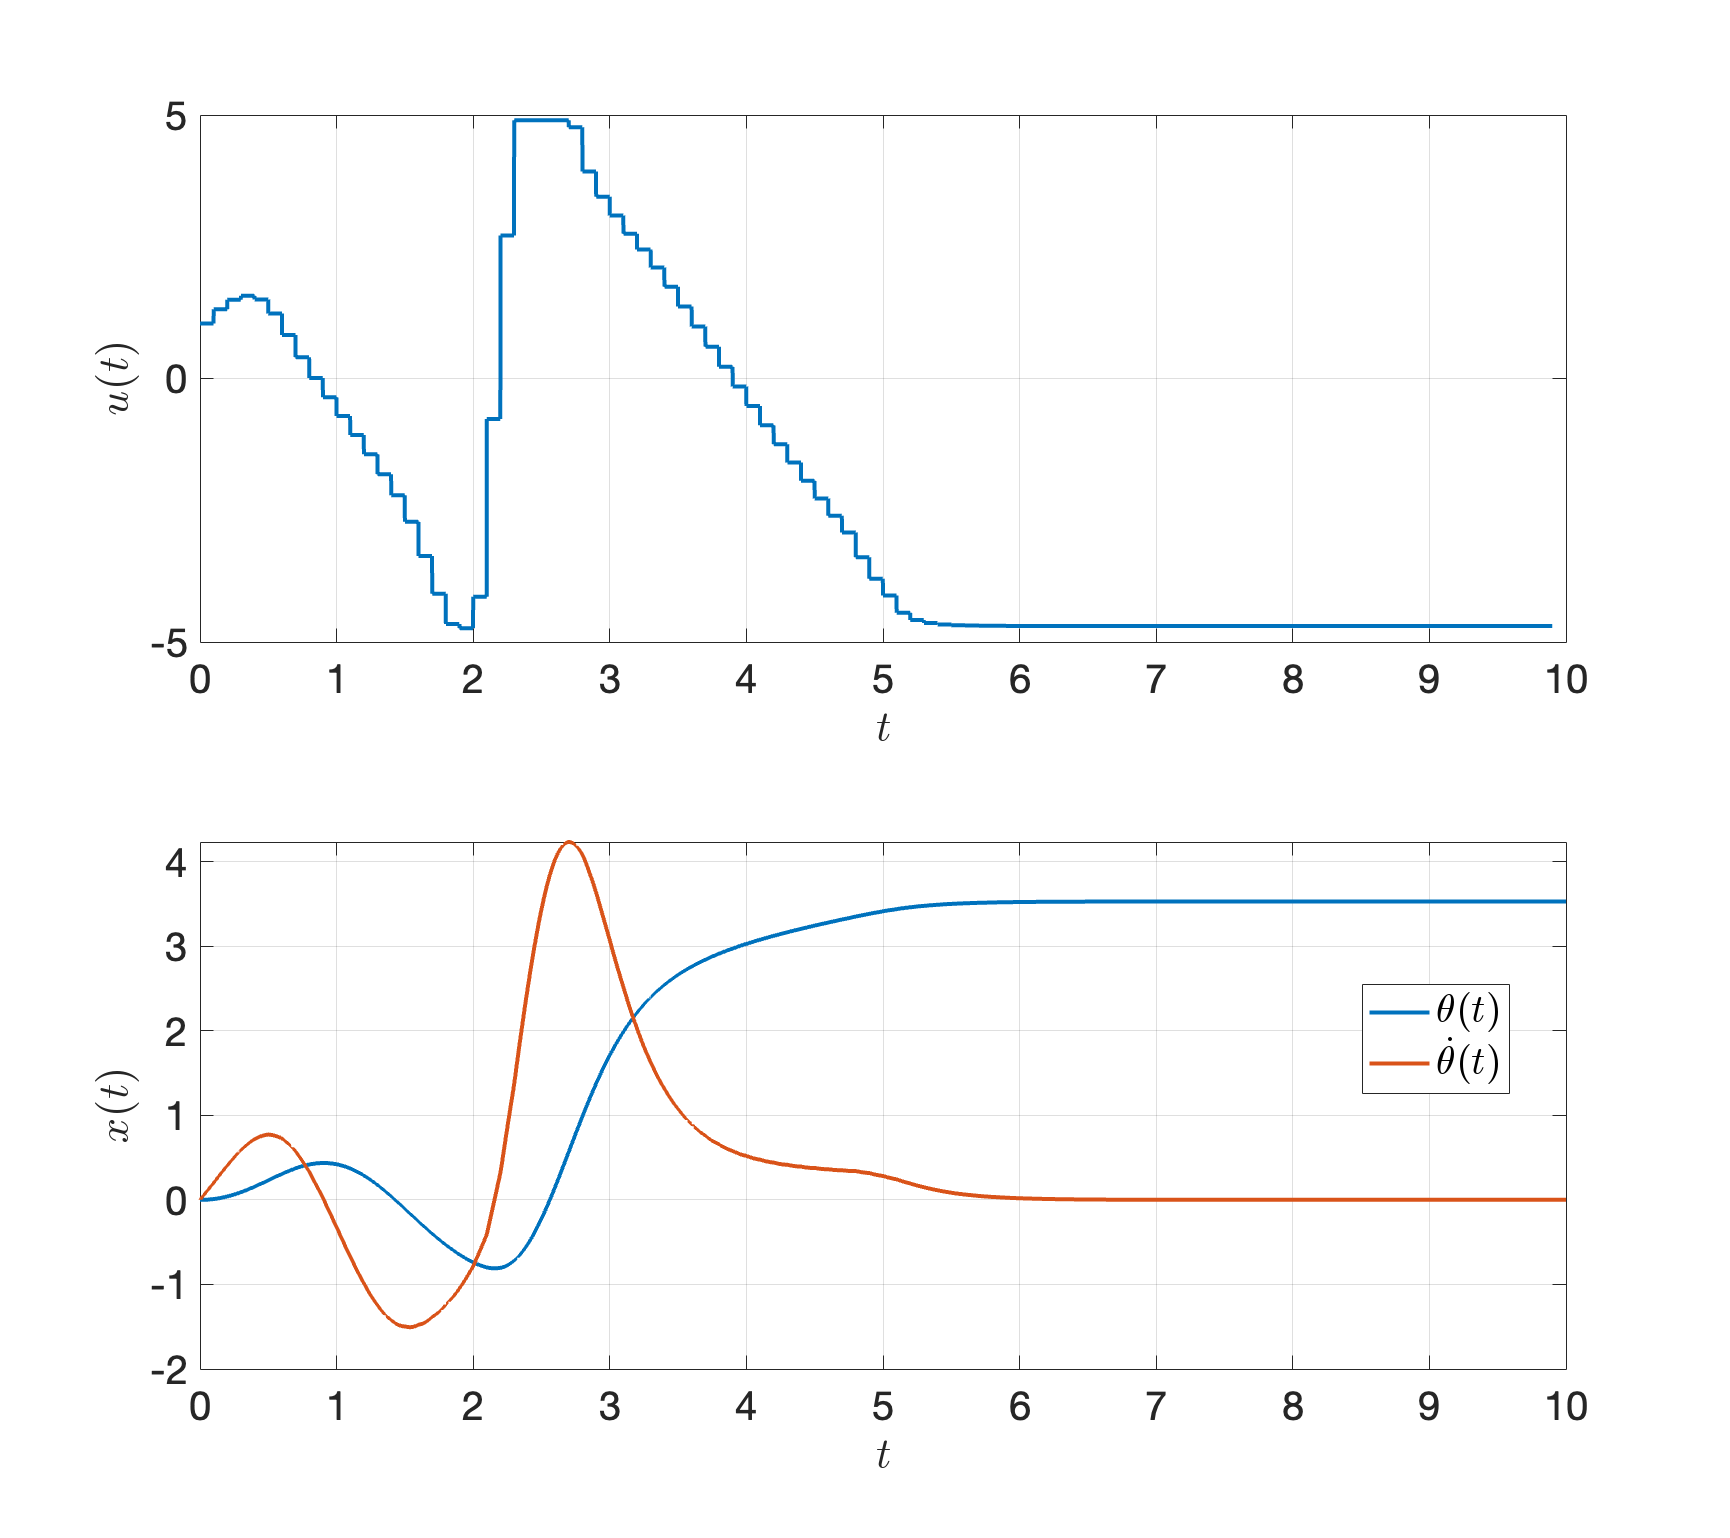
\includegraphics[width=0.8\linewidth]{images/pendulum_mpc_noise} 

}

\caption{MPC for pendulum swing-up with noise}\label{fig:pendulum-swingup-mpc-noise}
\end{figure}

Feel free to play with the code \href{https://github.com/ComputationalRobotics/OptimalControlEstimation-Examples/blob/main/pendulum_mpc/pendulum_mpc.m}{here}.
\end{example}

\textbf{Software tools}. Matlab implements a nice package for nonlinear MPC, you can refer to the \href{https://www.mathworks.com/help/mpc/ug/nonlinear-mpc.html}{documentation and examples}. In Python, the \href{https://www.do-mpc.com/en/latest/}{do-mpc package} is quite popular.

However, it is important to recognize that trajectory optimization for the nonconvex open-loop optimal control problen \eqref{eq:optimal-control-problem-mpc-open-loop} (a) only guarantees a locally optimal solution and hence can be brittle, (b) can be time-consuming when the problem is high-dimensional.

In fact, MPC was originally developed in the context of chemical plant control \citep{borrelli17book-mpc}, which has linear system dyanmics, as we will introduce soon. Before we introduce the MPC formulation and understand its theoretical properties, we need to take a detour and introduce various important notions of sets.

\hypertarget{controllability-reachability-and-invariance}{%
\subsection{Controllability, Reachability, and Invariance}\label{controllability-reachability-and-invariance}}

Consider the autonomous system
\begin{equation}
x_{t+1} = f_a(x_t)
\label{eq:mpc-autonomous-system}
\end{equation}
and the controlled system
\begin{equation}
x_{t+1} = f(x_t, u_t)
\label{eq:mpc-controlled-system}
\end{equation}
for \(t \geq 0\). Both systems are subject to state and input constraints
\begin{equation}
x_t \in \mathcal{X}, \quad u_t \in \mathcal{U}, \forall t \geq 0,
\label{eq:mpc-state-control-constraint}
\end{equation}
with \(\mathcal{X}\) and \(\mathcal{U}\) both being polyhedral sets (see Definition \ref{def:polyhedra})
\begin{equation}
\begin{split}
x_t \in \mathcal{X} = \left\{ x \in \mathbb{R}^n \mid C x \leq c \right\}, \quad C \in \mathbb{R}^{l_x \times n}, c \in \mathbb{R}^{l_x}, \\
u_t \in \mathcal{U} = \left\{ u \in \mathbb{R}^m \mid D u \leq d \right\}, \quad D \in \mathbb{R}^{l_u \times m}, d \in \mathbb{R}^{l_u}.
\end{split}
\label{eq:mpc-polyhedral-definition}
\end{equation}

We are going to make a few definitions.

\hypertarget{controllable-and-reachable-sets}{%
\subsubsection{Controllable and Reachable Sets}\label{controllable-and-reachable-sets}}

\begin{definition}[Precursor Set]
\protect\hypertarget{def:precursor-set}{}\label{def:precursor-set}For the autonomous system \eqref{eq:mpc-autonomous-system}, we define the precursor set to a set \(\mathcal{S}\) as
\[
\text{Pre}(\mathcal{S}) = \left\{ x \in \mathbb{R}^n \mid f_a(x) \in \mathcal{S} \right\}.
\]
In words, \(\text{Pre}(\mathcal{S})\) is the set of states which evolve into the target set \(\mathcal{S}\) in one time step.

For the controlled system \eqref{eq:mpc-controlled-system}, we define the precursor set to the set \(\mathcal{S}\) as
\[
\text{Pre}(\mathcal{S}) = \left\{ x \in \mathbb{R}^n : \exists u \in \mathcal{U} \text{  s.t. } f(x,u) \in \mathcal{S} \right\}.
\]
In words, \(\text{Pre}(\mathcal{S})\) is the set of states that can be driven into the target set \(\mathcal{S}\) while satisfying control and state constraints.
\end{definition}

A related concept is the successor set.

\begin{definition}[Successor Set]
\protect\hypertarget{def:successor-set}{}\label{def:successor-set}For the autonomous system \eqref{eq:mpc-autonomous-system}, we define the successor set to a set \(\mathcal{S}\) as
\[
\text{Suc}(\mathcal{S}) = \left\{ x \in \mathbb{R}^n \mid \exists x' \in \mathcal{S} \text{ s.t. } x = f_a(x')\right\}.
\]
In words, the states in \(\mathcal{S}\) get mapped into the states in \(\text{Suc}(\mathcal{S})\) after one time step.

For the controlled system \eqref{eq:mpc-controlled-system}, we define the successor set to the set \(\mathcal{S}\) as
\[
\text{Suc}(\mathcal{S}) = \left\{ x \in \mathbb{R}^n \mid \exists x' \in \mathcal{S}, \exists u' \in \mathcal{U} \text{ s.t. } x = f(x',u'). \right\}
\]
In words, the states in \(\mathcal{S}\) get mapped into the states in \(\text{Suc}(\mathcal{S})\) after one time step while satisfying the control constraints.
\end{definition}

The \(N\)-step controllable set is defined by iterating \(\text{Pre}(\cdot)\) computations.

\begin{definition}[N-Step Controllable Set]
\protect\hypertarget{def:controllable-set}{}\label{def:controllable-set}

Let \(\mathcal{S} \subseteq \mathcal{X}\) be a target set. The \(N\)-step controllable set \(\mathcal{K}_{N}(\mathcal{S})\) of the system \eqref{eq:mpc-autonomous-system} or \eqref{eq:mpc-controlled-system} subject to the constraints \eqref{eq:mpc-state-control-constraint} is defined recursively as:
\[
\mathcal{K}_0 (\mathcal{S}) = \mathcal{S}, \quad \mathcal{K}_{i}(\mathcal{S}) = \text{Pre}(\mathcal{K}_{i-1}(\mathcal{S})) \cap \mathcal{X}, i=1,\dots,N.
\]

According to this definition, given any \(x_0 \in \mathcal{K}_N(\mathcal{S})\):

\begin{itemize}
\item
  For the autonomous system \eqref{eq:mpc-autonomous-system}, its state will evolve into the target set \(\mathcal{S}\) in \(N\) steps while satisfying state constraints
\item
  For the controlled system \eqref{eq:mpc-controlled-system}, there exists a sequence of admissible controls (i.e., satisfying control constraints) such that its state will evolve into the target set \(\mathcal{S}\) in \(N\) steps while satisfying state constraints.
\end{itemize}

\end{definition}

Similarly, the \(N\)-step reachable set is defined by iterating \(\text{Suc}(\cdot)\) computations.

\begin{definition}[N-Step Reachable Set]
\protect\hypertarget{def:reachable-set}{}\label{def:reachable-set}

Let \(\mathcal{X}_0 \subseteq \mathcal{X}\) be an initial set. The \(N\)-step reachable set \(\mathcal{R}_N (\mathcal{X}_0)\) of the system \eqref{eq:mpc-autonomous-system} or \eqref{eq:mpc-controlled-system} subject to the constraints \eqref{eq:mpc-state-control-constraint} is defined recursively as:
\[
\mathcal{R}_0(\mathcal{X}_0) = \mathcal{X}_0, \quad \mathcal{R}_{i}(\mathcal{X}_0) = \text{Suc}(\mathcal{R}_{i-1}(\mathcal{X}_0)) \cap \mathcal{X}, i=1,\dots,N.
\]

According to this definition, given any \(x_0 \in \mathcal{X}_0\):

\begin{itemize}
\item
  For the autonomous system \eqref{eq:mpc-autonomous-system}, its state will evolve into \(\mathcal{R}_N(\mathcal{X}_0)\) in \(N\) steps while satisfying state constraints
\item
  For the controlled system \eqref{eq:mpc-controlled-system}, there exists a sequence of admissible controls (i.e., satisfying control constraints) such that its state will evolve into \(\mathcal{R}_N(\mathcal{X}_0)\) in \(N\) steps while satisfying state constraints.
\end{itemize}

\end{definition}

In the literature, the controllable set is often referred to as the \emph{backwards reachable set}.

\hypertarget{computation-of-controllable-and-reachable-sets}{%
\subsubsection{Computation of Controllable and Reachable Sets}\label{computation-of-controllable-and-reachable-sets}}

For a linear time-invariant system, when the state constraint set \(\mathcal{X}\), control constraint set \(\mathcal{U}\), the target set \(\mathcal{S}\), and the initial set \(\mathcal{X}_0\) are all polytopes, then the \(N\)-step controllable set \(\mathcal{K}_{N}(\mathcal{S})\) and the \(N\)-step reachable set \(\mathcal{R}_{N}(\mathcal{X}_0)\) are both polytopes and can be computed exactly and efficiently.

We will not describe the underlying algorithm for computing \(\mathcal{K}_{N}(\mathcal{S})\) and \(\mathcal{R}_{N}(\mathcal{X}_0)\) (these details can be found in \citep{borrelli17book-mpc} and they are not very difficult to understand, so I suggest you to read them), but we now show you how to use the \href{https://www.mpt3.org/}{Multi-Parametric Toolbox (MPT)} to compute them.

\begin{example}[Compute Controllable and Reachable Sets]
\protect\hypertarget{exm:compute-controllable-reachable-sets}{}\label{exm:compute-controllable-reachable-sets}

Consider a linear system
\[
x_{t+1} = \begin{bmatrix} 1.5 & 0 \\ 1 & -1.5 \end{bmatrix} x_t + \begin{bmatrix} 1 \\ 0 \end{bmatrix} u_t
\]
with state and control constraints
\[
\mathcal{X} = [-10,10]^2, \quad \mathcal{U} = [-5,5].
\]
Given \(\mathcal{S} = \mathcal{X}_0 = [-1,1]^2\), I want to compute \(\mathcal{K}_i(\mathcal{S})\) and \(\mathcal{R}_i(\mathcal{X}_0)\), for \(i=0,1,2,3,4\).

\textbf{Dynamical system}. We first define the linear time-invariant system as follows.

\begin{Shaded}
\begin{Highlighting}[]
\VariableTok{A} \OperatorTok{=}\NormalTok{ [}\FloatTok{1.5}\OperatorTok{,} \FloatTok{0}\OperatorTok{;} \FloatTok{1}\OperatorTok{,} \OperatorTok{{-}}\FloatTok{1.5}\NormalTok{]}\OperatorTok{;} \VariableTok{B} \OperatorTok{=}\NormalTok{ [}\FloatTok{1}\OperatorTok{;} \FloatTok{0}\NormalTok{]}\OperatorTok{;}
\VariableTok{sys} \OperatorTok{=} \VariableTok{LTISystem}\NormalTok{(}\SpecialStringTok{\textquotesingle{}A\textquotesingle{}}\OperatorTok{,}\VariableTok{A}\OperatorTok{,}\SpecialStringTok{\textquotesingle{}B\textquotesingle{}}\OperatorTok{,}\VariableTok{B}\NormalTok{)}\OperatorTok{;}
\end{Highlighting}
\end{Shaded}

We then define the state and control constraints.

\begin{Shaded}
\begin{Highlighting}[]
\VariableTok{calX} \OperatorTok{=} \VariableTok{Polyhedron}\NormalTok{(}\SpecialStringTok{\textquotesingle{}A\textquotesingle{}}\OperatorTok{,...}
\NormalTok{    [}\FloatTok{1}\OperatorTok{,}\FloatTok{0}\OperatorTok{;}\FloatTok{0}\OperatorTok{,}\FloatTok{1}\OperatorTok{;{-}}\FloatTok{1}\OperatorTok{,}\FloatTok{0}\OperatorTok{;}\FloatTok{0}\OperatorTok{,{-}}\FloatTok{1}\NormalTok{]}\OperatorTok{,} \OperatorTok{...}
    \SpecialStringTok{\textquotesingle{}b\textquotesingle{}}\OperatorTok{,}\NormalTok{[}\FloatTok{10}\OperatorTok{;}\FloatTok{10}\OperatorTok{;}\FloatTok{10}\OperatorTok{;}\FloatTok{10}\NormalTok{])}\OperatorTok{;}
\VariableTok{calU} \OperatorTok{=} \VariableTok{Polyhedron}\NormalTok{(}\SpecialStringTok{\textquotesingle{}A\textquotesingle{}}\OperatorTok{,}\NormalTok{[}\FloatTok{1}\OperatorTok{;{-}}\FloatTok{1}\NormalTok{]}\OperatorTok{,}\SpecialStringTok{\textquotesingle{}b\textquotesingle{}}\OperatorTok{,}\NormalTok{[}\FloatTok{5}\OperatorTok{;}\FloatTok{5}\NormalTok{])}\OperatorTok{;}
\end{Highlighting}
\end{Shaded}

Note that in the MPT toolbox, to define a polytope \(P = \{ x \in \mathbb{R}^n \mid A x \leq b \}\), we just need to call the \texttt{Polyhedron} function with inputs \texttt{A} and \texttt{b}.

\textbf{Controllable sets}. We have from Definition \ref{def:controllable-set} the recursion
\[
\mathcal{K}_0(\mathcal{S}) = \mathcal{S}, \quad \mathcal{K}_i(\mathcal{S}) = \text{Pre}(\mathcal{K}_{i-1}(\mathcal{S})) \cap \mathcal{X}.
\]
To implement the above set operation, we need two functions, one for the ``\(\cap\)'' intersection operation, and the other for the ``\(\text{Pre}(\cdot)\)'' precursor set operation. These two functions are both available through MPT.

\begin{itemize}
\item
  \texttt{intersect(P,S)} computes the intersection of two sets \texttt{P} and \texttt{S}, both defined as polytopes.
\item
  \texttt{system.reachableSet(\textquotesingle{}X\textquotesingle{},\ X,\ \textquotesingle{}U\textquotesingle{},\ U,\ \textquotesingle{}N\textquotesingle{},\ 1,\ \textquotesingle{}direction\textquotesingle{},\ \textquotesingle{}backwards\textquotesingle{})} computes the one-step backwards reachable set (which is just the precursor set) of the \texttt{system} with target set \texttt{X} and control constraints \texttt{U}.
\end{itemize}

Using these two functions, the following code snippet computes recursively the controllable sets for \(N\) steps.

\begin{Shaded}
\begin{Highlighting}[]
\CommentTok{\% target set}
\VariableTok{S} \OperatorTok{=} \VariableTok{Polyhedron}\NormalTok{(}\SpecialStringTok{\textquotesingle{}A\textquotesingle{}}\OperatorTok{,}\NormalTok{[}\FloatTok{1}\OperatorTok{,}\FloatTok{0}\OperatorTok{;}\FloatTok{0}\OperatorTok{,}\FloatTok{1}\OperatorTok{;{-}}\FloatTok{1}\OperatorTok{,}\FloatTok{0}\OperatorTok{;}\FloatTok{0}\OperatorTok{,{-}}\FloatTok{1}\NormalTok{]}\OperatorTok{,}\SpecialStringTok{\textquotesingle{}b\textquotesingle{}}\OperatorTok{,}\NormalTok{[}\FloatTok{1}\OperatorTok{;}\FloatTok{1}\OperatorTok{;}\FloatTok{1}\OperatorTok{;}\FloatTok{1}\NormalTok{])}\OperatorTok{;}
\VariableTok{K} \OperatorTok{=}\NormalTok{ [}\VariableTok{S}\NormalTok{]}\OperatorTok{;}
\VariableTok{N} \OperatorTok{=} \FloatTok{4}\OperatorTok{;}
\KeywordTok{for} \VariableTok{i} \OperatorTok{=} \FloatTok{1}\OperatorTok{:}\VariableTok{N}
    \VariableTok{Si} \OperatorTok{=} \VariableTok{sys}\NormalTok{.}\VariableTok{reachableSet}\NormalTok{(}\SpecialStringTok{\textquotesingle{}X\textquotesingle{}}\OperatorTok{,}\VariableTok{K}\NormalTok{(}\VariableTok{i}\NormalTok{)}\OperatorTok{,}\SpecialStringTok{\textquotesingle{}U\textquotesingle{}}\OperatorTok{,}\VariableTok{calU}\OperatorTok{,}\SpecialStringTok{\textquotesingle{}N\textquotesingle{}}\OperatorTok{,}\FloatTok{1}\OperatorTok{,}\SpecialStringTok{\textquotesingle{}direction\textquotesingle{}}\OperatorTok{,}\SpecialStringTok{\textquotesingle{}backwards\textquotesingle{}}\NormalTok{)}\OperatorTok{;}
    \VariableTok{K} \OperatorTok{=}\NormalTok{ [}\VariableTok{K}\OperatorTok{;} \VariableTok{intersect}\NormalTok{(}\VariableTok{Si}\OperatorTok{,}\VariableTok{calX}\NormalTok{)]}\OperatorTok{;}
\KeywordTok{end}
\end{Highlighting}
\end{Shaded}

Fig. \ref{fig:controllable-set-example} plots the controllable sets computed by running the above code.

\begin{figure}

{\centering 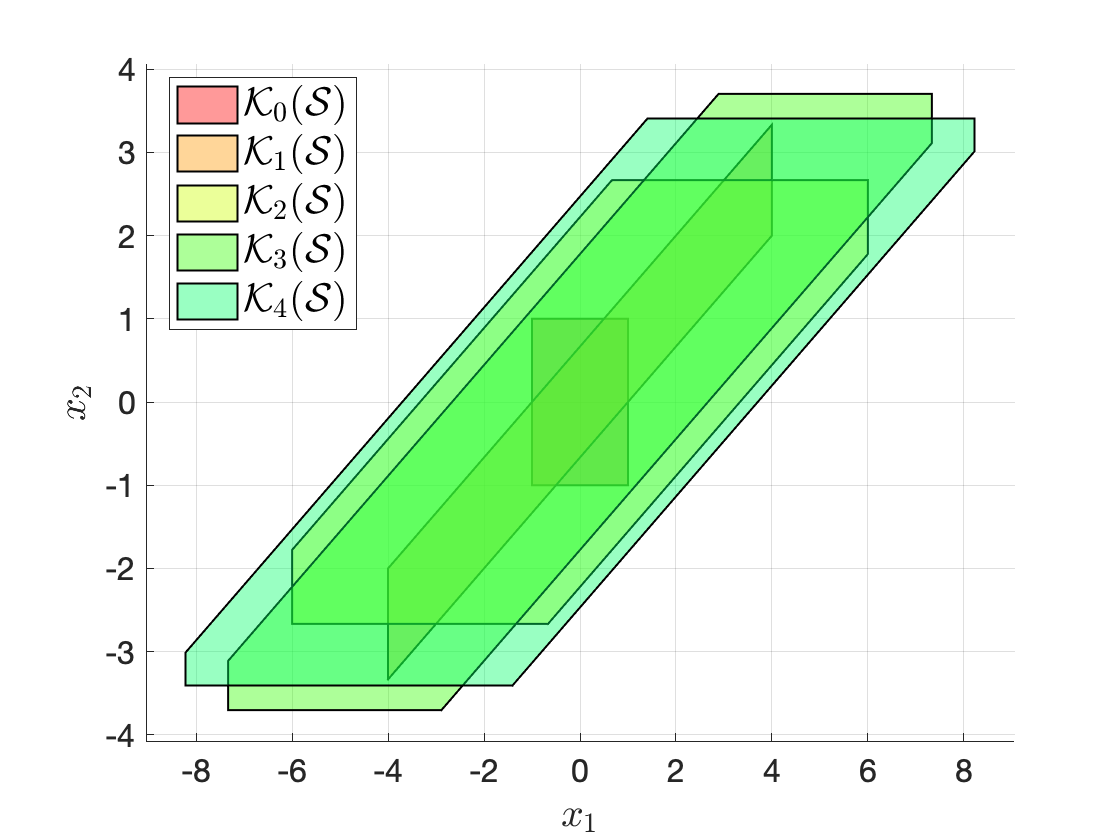
\includegraphics[width=0.6\linewidth]{images/controllable_set_overlap} 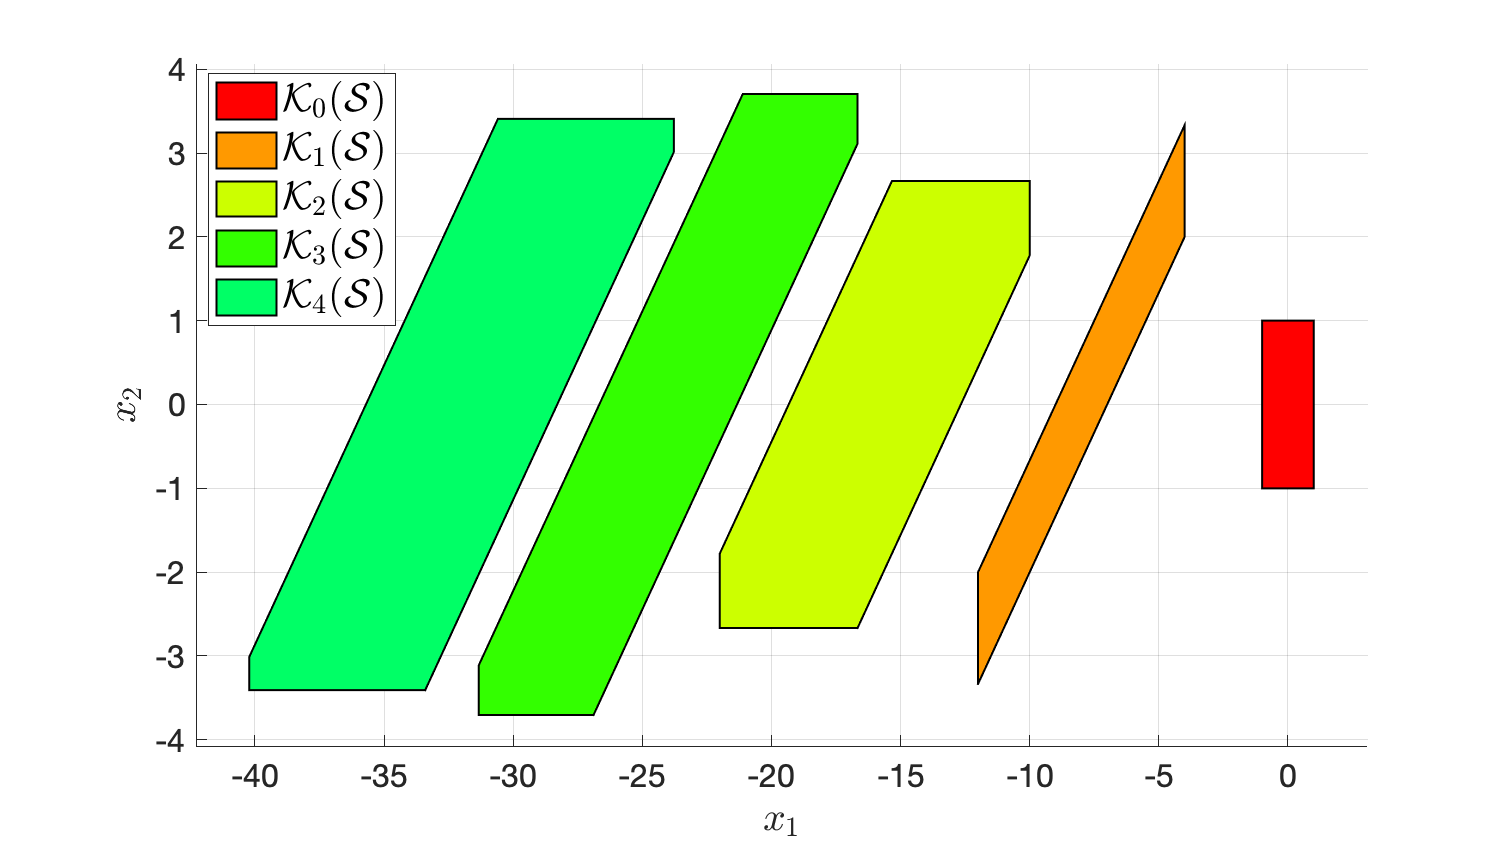
\includegraphics[width=0.6\linewidth]{images/controllable_set_shift} 

}

\caption{Computation of controllable sets using MPT. The bottom plot shifts the sets horizontally for better visualization.}\label{fig:controllable-set-example}
\end{figure}

\textbf{Reachable sets}. We have Definition \ref{def:reachable-set} the recursion
\[
\mathcal{R}_0(\mathcal{X}_0) = \mathcal{X}_0, \quad \mathcal{R}_i(\mathcal{X}_0) = \text{Suc}(\mathcal{R}_{i-1}(\mathcal{X}_0)) \cap \mathcal{X}.
\]
To implement the recursion above, we need ``\(\cap\)'' set intersection, which is available via \texttt{intersect(P,S)}, and the ``\(\text{Suc}(\cdot)\)'' successor set operation, which is available as

\begin{itemize}
\tightlist
\item
  \texttt{system.reachableSet(\textquotesingle{}X\textquotesingle{},\ X,\ \textquotesingle{}U\textquotesingle{},\ U,\ \textquotesingle{}N\textquotesingle{},\ 1,\ \textquotesingle{}direction\textquotesingle{},\ \textquotesingle{}forward\textquotesingle{})} computes the one-step forward reachable set (which is just the successor set) of the \texttt{system} with initial set \texttt{X} and control constraints \texttt{U}.
\end{itemize}

Therefore, we can compute the reachable sets recursively using the following code snippet

\begin{Shaded}
\begin{Highlighting}[]
\CommentTok{\% initial set}
\VariableTok{X0} \OperatorTok{=} \VariableTok{Polyhedron}\NormalTok{(}\SpecialStringTok{\textquotesingle{}A\textquotesingle{}}\OperatorTok{,}\NormalTok{[}\FloatTok{1}\OperatorTok{,}\FloatTok{0}\OperatorTok{;}\FloatTok{0}\OperatorTok{,}\FloatTok{1}\OperatorTok{;{-}}\FloatTok{1}\OperatorTok{,}\FloatTok{0}\OperatorTok{;}\FloatTok{0}\OperatorTok{,{-}}\FloatTok{1}\NormalTok{]}\OperatorTok{,}\SpecialStringTok{\textquotesingle{}b\textquotesingle{}}\OperatorTok{,}\NormalTok{[}\FloatTok{1}\OperatorTok{;}\FloatTok{1}\OperatorTok{;}\FloatTok{1}\OperatorTok{;}\FloatTok{1}\NormalTok{])}\OperatorTok{;}
\VariableTok{R} \OperatorTok{=}\NormalTok{ [}\VariableTok{X0}\NormalTok{]}\OperatorTok{;}
\VariableTok{N} \OperatorTok{=} \FloatTok{4}\OperatorTok{;}
\KeywordTok{for} \VariableTok{i} \OperatorTok{=} \FloatTok{1}\OperatorTok{:}\VariableTok{N}
    \VariableTok{Ri} \OperatorTok{=} \VariableTok{sys}\NormalTok{.}\VariableTok{reachableSet}\NormalTok{(}\SpecialStringTok{\textquotesingle{}X\textquotesingle{}}\OperatorTok{,}\VariableTok{R}\NormalTok{(}\VariableTok{i}\NormalTok{)}\OperatorTok{,}\SpecialStringTok{\textquotesingle{}U\textquotesingle{}}\OperatorTok{,}\VariableTok{calU}\OperatorTok{,}\SpecialStringTok{\textquotesingle{}N\textquotesingle{}}\OperatorTok{,}\FloatTok{1}\OperatorTok{,}\SpecialStringTok{\textquotesingle{}direction\textquotesingle{}}\OperatorTok{,}\SpecialStringTok{\textquotesingle{}forward\textquotesingle{}}\NormalTok{)}\OperatorTok{;}
    \VariableTok{R} \OperatorTok{=}\NormalTok{ [}\VariableTok{R}\OperatorTok{;} \VariableTok{intersect}\NormalTok{(}\VariableTok{Ri}\OperatorTok{,}\VariableTok{calX}\NormalTok{)]}\OperatorTok{;}
\KeywordTok{end}
\end{Highlighting}
\end{Shaded}

Fig. \ref{fig:reachable-set-example} plots the reachable sets computed by running the above code.

Feel free to play with the code \href{https://github.com/ComputationalRobotics/OptimalControlEstimation-Examples/blob/main/mpt_examples/controllable_reachable_sets.m}{here}. Note that you need to \href{https://www.mpt3.org/Main/Installation}{install the MPT toolbox} before running the code.

\begin{figure}

{\centering 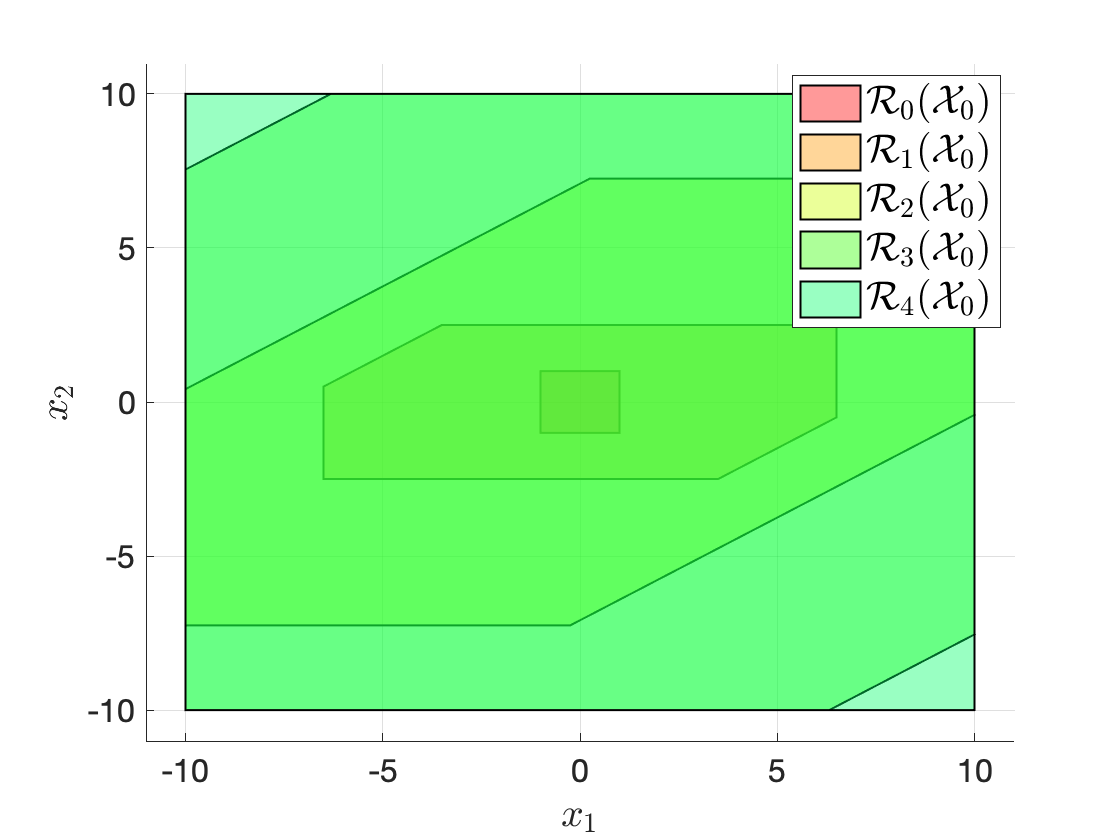
\includegraphics[width=0.6\linewidth]{images/reachable_set_overlap} 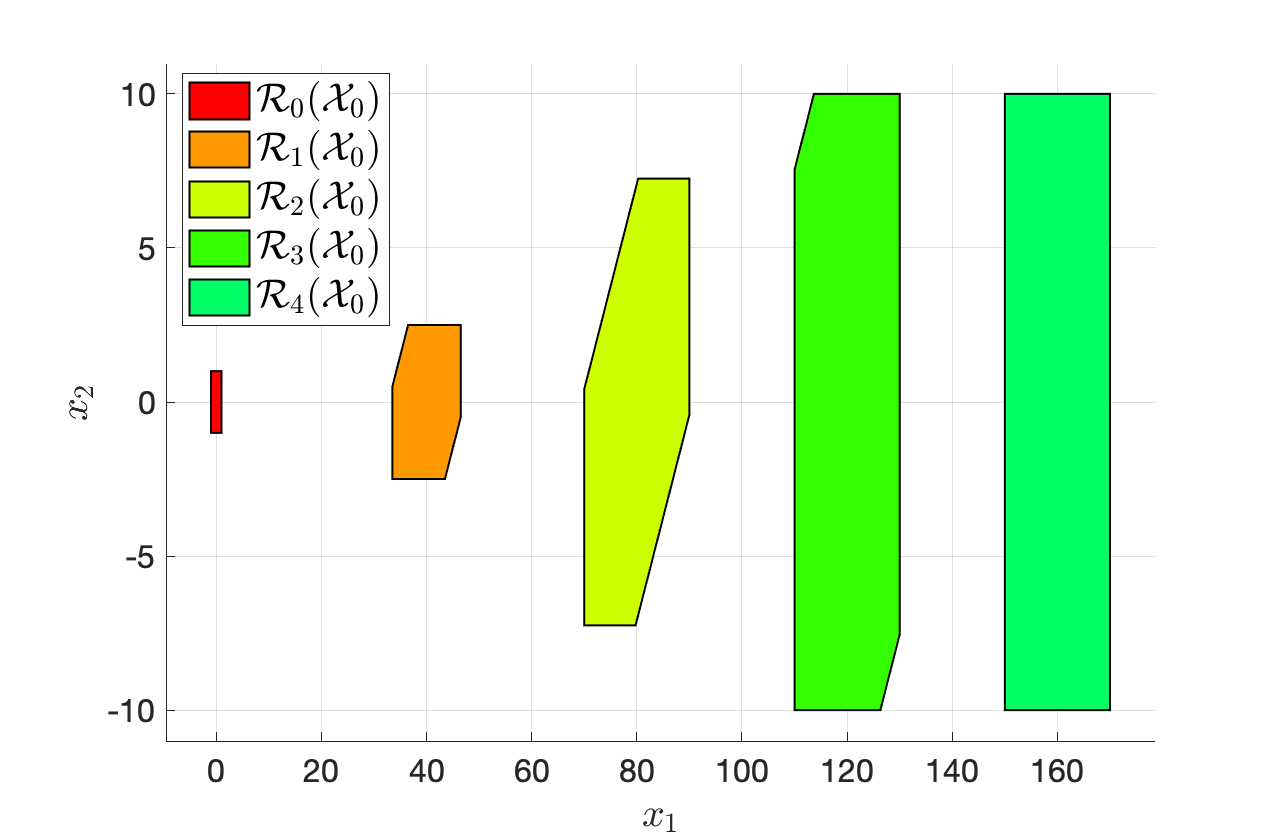
\includegraphics[width=0.6\linewidth]{images/reachable_set_shift} 

}

\caption{Computation of reachable sets using MPT. The bottom plot shifts the sets horizontally for better visualization.}\label{fig:reachable-set-example}
\end{figure}

\end{example}

\hypertarget{invariant-sets}{%
\subsubsection{Invariant Sets}\label{invariant-sets}}

\begin{definition}[Positive Invariant Set]
\protect\hypertarget{def:positive-invariant-set}{}\label{def:positive-invariant-set}A set \(\mathcal{O} \subseteq \mathcal{X}\) is said to be a positive invariant set for the autonomous system \eqref{eq:mpc-autonomous-system} subject to the constraints in \eqref{eq:mpc-state-control-constraint} if
\[
x_0 \in \mathcal{O} \Longrightarrow x_t \in \mathcal{O}, \forall t \geq 0.
\]
That is, if the system starts in \(\mathcal{O}\), it stays in \(\mathcal{O}\) for all future timesteps.
\end{definition}

The maximal positive invariant set is the largest positive invariant set.

\begin{definition}[Maximal Positive Invariant Set]
\protect\hypertarget{def:maximal-positive-invariant-set}{}\label{def:maximal-positive-invariant-set}A set \(\mathcal{O}_{\infty} \subseteq \mathcal{X}\) is said to be the maximal positive invariant set for the autonomous system \eqref{eq:mpc-autonomous-system} subject to the constraints in \eqref{eq:mpc-state-control-constraint} if (a) \(\mathcal{O}_{\infty}\) is positive invariant and (b) \(\mathcal{O}_{\infty}\) contains all the invariant sets contained in \(\mathcal{X}\).
\end{definition}

Essentially, the (maximal) positive invariant set is the set of initial conditions under which the system does not blow up.

For the controlled system \eqref{eq:mpc-controlled-system}, we have the similar notion of a control invariant set.

\begin{definition}[Control Invariant Set]
\protect\hypertarget{def:control-invariant-set}{}\label{def:control-invariant-set}A set \(\mathcal{C} \subseteq \mathcal{X}\) is said to be a control invariant set for the controlled system \eqref{eq:mpc-controlled-system} subject to the constraints in \eqref{eq:mpc-state-control-constraint} if
\[
x_0 \in \mathcal{C} \Longrightarrow \exists u_t \in \mathcal{U} \text{ s.t. } f(x_t,u_t) \in \mathcal{C}, \forall t \geq 0
\]
That is, if the system starts in \(\mathcal{C}\), it can be controlled to stay in \(\mathcal{C}\) for all future time steps.
\end{definition}

The maximal control invariant set is the largest control invariant set.

\begin{definition}[Maximal Control Invariant Set]
\protect\hypertarget{def:maximal-control-invariant-set}{}\label{def:maximal-control-invariant-set}A set \(\mathcal{C}_{\infty} \subseteq \mathcal{X}\) is said to be the maximal control invariant set for the controlled system \eqref{eq:mpc-controlled-system} subject to the constraints in \eqref{eq:mpc-state-control-constraint} if (a) \(\mathcal{C}_{\infty}\) is control invariant, and (b) \(\mathcal{C}_{\infty}\) contains all control invariant sets contained in \(\mathcal{X}\).
\end{definition}

Essentially, the (maximal) control invariant set is the set of initial conditions under which the system can be controlled to not blow up.

We now state a necessary and sufficient condition for a set to be positive invariant and control invariant.

\begin{theorem}[Geometric Condition for Invariance]
\protect\hypertarget{thm:geometric-condition-for-invariance}{}\label{thm:geometric-condition-for-invariance}For the autonomous system \eqref{eq:mpc-autonomous-system} subject to the constraint \eqref{eq:mpc-state-control-constraint}, a set \(\mathcal{O} \subseteq \mathcal{X}\) is positive invariant if and only if
\begin{equation}
\mathcal{O} \subseteq \text{Pre}(\mathcal{O}).
\label{eq:positive-invariant-geometric}
\end{equation}

Similarly, for the controlled system \eqref{eq:mpc-controlled-system} subject to the constraint \eqref{eq:mpc-state-control-constraint}, a set \(\mathcal{C}\) is control invariant if and only if
\begin{equation}
\mathcal{C} \subseteq \text{Pre}(\mathcal{C}).
\label{eq:control-invariant-geometric}
\end{equation}
\end{theorem}

\begin{proof}
We only prove \eqref{eq:positive-invariant-geometric} since \eqref{eq:control-invariant-geometric} can be proved using similar arguments.

\begin{itemize}
\item
  ``\(\Leftarrow\)'': we want to show \(\mathcal{O}\) is positive invariant if \eqref{eq:positive-invariant-geometric} holds. We prove this by contradiction. If \(\mathcal{O}\) is not positive invariant, the \(\exists \hat{x} \in \mathcal{O}\) such that \(f_a(\hat{x}) \not\in \mathcal{O}\). This implies we have found \(\hat{x} \in \mathcal{O}\) but \(\hat{x} \not\in \text{Pre}(\mathcal{O})\), contradicting \eqref{eq:positive-invariant-geometric}.
\item
  ``\(\Rightarrow\)'': we want to show \eqref{eq:positive-invariant-geometric} holds if \(\mathcal{O}\) is positive invariant. We prove this by contradiction. Suppose \eqref{eq:positive-invariant-geometric} does not hold, then \(\exists \hat{x}\) such that \(\hat{x} \in \mathcal{O}\) but \(\hat{x} \not\in \text{Pre}(\mathcal{O})\). This implies we have found \(\hat{x} \in \mathcal{O}\) that does not remain in \(\mathcal{O}\) in the next step, contradicting \(\mathcal{O}\) being positive invariant.
\end{itemize}

This shows that \eqref{eq:positive-invariant-geometric} is a sufficient and necessary condition.
\end{proof}

Theorem \ref{thm:geometric-condition-for-invariance} immediately suggests an algoithm for computing (control) invariant sets, as we will describe in the next section.

\hypertarget{mpc-compute-control-invariant-set}{%
\subsubsection{Computation of Invariant Sets}\label{mpc-compute-control-invariant-set}}

Observe that the geometric conditions \eqref{eq:positive-invariant-geometric} and \eqref{eq:control-invariant-geometric} are equivalent to the following conditions
\[
\mathcal{O} = \text{Pre}(\mathcal{O}) \cap \mathcal{O}, \quad \mathcal{C} = \text{Pre}(\mathcal{C}) \cap \mathcal{C}.
\]

Based on the equation above, we can design an algoithm that iteratively evaluates \(\text{Pre}(\mathcal{\Omega}) \cap \mathcal{\Omega}\) until it converges.

\begin{center}\rule{0.5\linewidth}{0.5pt}\end{center}

\textbf{Algorithm}: Computation of \(\mathcal{O}_{\infty}\)

\begin{center}\rule{0.5\linewidth}{0.5pt}\end{center}

\textbf{Input:} \(f_a\), \(\mathcal{X}\)

\textbf{Output:} \(\mathcal{O}_{\infty}\)

~~ \(\Omega_0 \leftarrow \mathcal{X}\), \(k=0\)

~~ \textbf{Repeat}

~~~~ \(\Omega_{k+1} \leftarrow \text{Pre}(\Omega_k) \cap \Omega_k\)

~~~~ \(k \leftarrow k+1\)

~~ \textbf{Until} \(\Omega_{k+1} = \Omega_k\).

~~ \(\mathcal{O}_{\infty} \leftarrow \Omega_k\)

\begin{center}\rule{0.5\linewidth}{0.5pt}\end{center}

The algorithm above generates a sequence of sets \(\{ \Omega_k \}\) satisfying \(\Omega_{k+1} \subseteq \Omega_k\) for any \(k\), and it terminates when \(\Omega_{k+1} = \Omega_k\). If it terminates, then \(\Omega_k\) is the maximal positive invariant set \(\mathcal{O}_{\infty}\). If \(\Omega_k = \emptyset\) for some intege \(k\) then \(\mathcal{O}_{\infty} = \emptyset\).

In general, the algoithm above may never terminate. If the algoithm does not terminate in a finite number of iterations, then it can be proven that \citep{kolmanovsky98mpe-theory}
\[
\mathcal{O}_{\infty} = \lim_{k \rightarrow \infty} \Omega_k.
\]

Conditions for finite time termination of the algoithm can be found in \citep{gilbert91tac-linear}. A simple sufficient condition requires the dynamics \(f_a\) to be linear and stable, and the constraint set \(\mathcal{X}\) to be bounded and contain the origin.

The same algoithm can be used to compute the maximal control invariant set \(\mathcal{C}_{\infty}\).

\begin{center}\rule{0.5\linewidth}{0.5pt}\end{center}

\textbf{Algorithm}: Computation of \(\mathcal{C}_{\infty}\)

\begin{center}\rule{0.5\linewidth}{0.5pt}\end{center}

\textbf{Input:} \(f\), \(\mathcal{X}\), \(\mathcal{U}\)

\textbf{Output:} \(\mathcal{C}_{\infty}\)

~~ \(\Omega_0 \leftarrow \mathcal{X}\), \(k=0\)

~~ \textbf{Repeat}

~~~~ \(\Omega_{k+1} \leftarrow \text{Pre}(\Omega_k) \cap \Omega_k\)

~~~~ \(k \leftarrow k+1\)

~~ \textbf{Until} \(\Omega_{k+1} = \Omega_k\).

~~ \(\mathcal{C}_{\infty} \leftarrow \Omega_k\)

\begin{center}\rule{0.5\linewidth}{0.5pt}\end{center}

Similarly, the above algoithm generates \(\{\Omega_k \}\) such that \(\Omega_{k+1} \subseteq \Omega_k\) for any \(k\). If the algoithm terminates, then \(\Omega_k = \mathcal{C}_{\infty}\).

In general, the algoithm may never terminate. If the algoithm does not terminate, then in general convergence is not guaranteed
\[
\mathcal{C}_{\infty} \neq \lim_{k \rightarrow \infty} \Omega_k.
\]
The work in \citep{bertsekas72tac-infinite} reports examples of nonlinear systems for which the above equation can be observed. A sufficient condition for the convergence of \(\Omega_k\) to \(\mathcal{C}_{\infty}\) as \(k \rightarrow \infty\) requires the polyhedral sets \(\mathcal{X}\) and \(\mathcal{U}\) to be bounded and the system \(f(x,u)\) to be continuous \citep{bertsekas72tac-infinite}.

Let us apply the algoithm to compute the maximal control invariant set for the linear system in Example \ref{exm:compute-controllable-reachable-sets}.

\begin{example}[Computation of the Maximal Control Invariant Set]
\protect\hypertarget{exm:compute-control-invariant-set}{}\label{exm:compute-control-invariant-set}Consider the linear system in Example \ref{exm:compute-controllable-reachable-sets} with same state constraint and control constraint.

The following code snippet shows how to apply the iterative algorithm introduced above to compute the maximal control invariant set.

\begin{Shaded}
\begin{Highlighting}[]
\VariableTok{Omega} \OperatorTok{=}\NormalTok{ [}\VariableTok{calX}\NormalTok{]}\OperatorTok{;}
\KeywordTok{while} \VariableTok{true}
    \VariableTok{last\_Omega} \OperatorTok{=} \VariableTok{Omega}\NormalTok{(}\KeywordTok{end}\NormalTok{)}\OperatorTok{;}
    \VariableTok{pre\_omega} \OperatorTok{=} \VariableTok{sys}\NormalTok{.}\VariableTok{reachableSet}\NormalTok{(}\SpecialStringTok{\textquotesingle{}X\textquotesingle{}}\OperatorTok{,}\VariableTok{last\_Omega}\OperatorTok{,}\SpecialStringTok{\textquotesingle{}U\textquotesingle{}}\OperatorTok{,}\VariableTok{calU}\OperatorTok{,}\SpecialStringTok{\textquotesingle{}N\textquotesingle{}}\OperatorTok{,}\FloatTok{1}\OperatorTok{,...}
        \SpecialStringTok{\textquotesingle{}direction\textquotesingle{}}\OperatorTok{,}\SpecialStringTok{\textquotesingle{}backwards\textquotesingle{}}\NormalTok{)}\OperatorTok{;}
    \VariableTok{new\_Omega} \OperatorTok{=} \VariableTok{intersect}\NormalTok{(}\VariableTok{pre\_omega}\OperatorTok{,}\VariableTok{last\_Omega}\NormalTok{)}\OperatorTok{;}
    \VariableTok{Omega} \OperatorTok{=}\NormalTok{ [}\VariableTok{Omega}\OperatorTok{;}\VariableTok{new\_Omega}\NormalTok{]}\OperatorTok{;}
    \KeywordTok{if} \VariableTok{new\_Omega} \OperatorTok{==} \VariableTok{last\_Omega}
        \VariableTok{fprintf}\NormalTok{(}\StringTok{"Converged to maximal control invariant set.\textbackslash{}n"}\NormalTok{)}\OperatorTok{;}
        \KeywordTok{break}\OperatorTok{;}
    \KeywordTok{end}
\KeywordTok{end}
\end{Highlighting}
\end{Shaded}

The algoithm converges in 37 iterations and Fig. \ref{fig:max-control-invariant-set} plots the sequence of sets generated by the algorithm.

\begin{figure}

{\centering 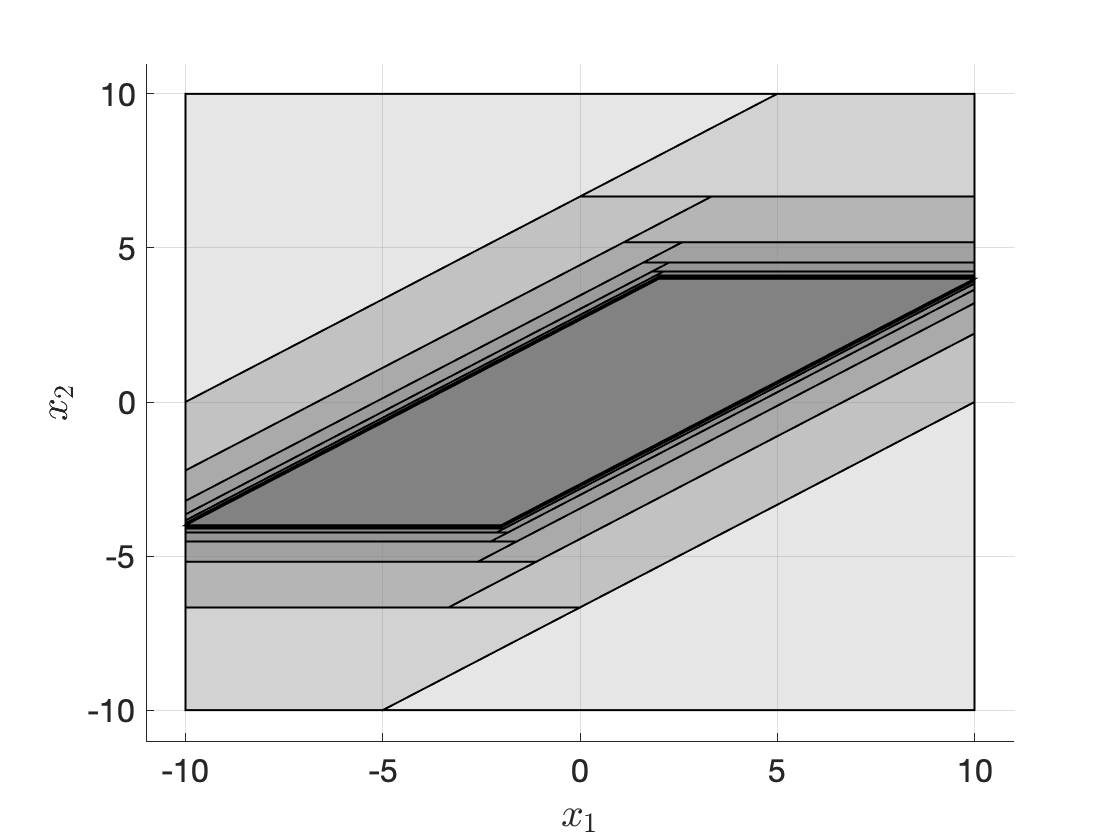
\includegraphics[width=0.6\linewidth]{images/maximal_control_invariant_set} 

}

\caption{Maximal control invariant set.}\label{fig:max-control-invariant-set}
\end{figure}

The MPT toolbox actually implements this algoithm for us to use directly. If we use

\begin{Shaded}
\begin{Highlighting}[]
\VariableTok{C} \OperatorTok{=} \VariableTok{sys}\NormalTok{.}\VariableTok{invariantSet}\NormalTok{(}\SpecialStringTok{\textquotesingle{}X\textquotesingle{}}\OperatorTok{,} \VariableTok{calX}\OperatorTok{,} \SpecialStringTok{\textquotesingle{}U\textquotesingle{}}\OperatorTok{,} \VariableTok{calU}\NormalTok{)}\OperatorTok{;}
\end{Highlighting}
\end{Shaded}

we get the same result as before.

You can play with the code \href{https://github.com/ComputationalRobotics/OptimalControlEstimation-Examples/blob/main/mpt_examples/maximal_control_invariant_set.m}{here}.
\end{example}

\hypertarget{basic-formulation-for-linear-systems}{%
\subsection{Basic Formulation for Linear Systems}\label{basic-formulation-for-linear-systems}}

We are now ready to introduce the basic formulation of MPC for linear systems and study its theoretical properties.

Consider the problem of regulating the following discrete-time linear system to the origin
\begin{equation}
x_{t+1} = A x_t + B u_t,
\label{eq:mpc-linear-system}
\end{equation}
where the state \(x_t\) and control \(u_t\) are constrained to lie in polyhedral sets \(\mathcal{X}\) and \(\mathcal{U}\), respectively.
We assume \(\mathcal{X}\) contains the origin \(0\).

We can formulate the following optimal control problem to regulate the system to the origin
\begin{equation}
\begin{split}
J^\star(x_0) = \min_{u_t,t=0,\dots} & \quad \sum_{t=0}^{\infty} x_t^T Q x_t + u_t^T R u_t \\
\text{subject to} & \quad x_{t+1} = A x_t + B u_t, \\
& \quad (u_t,x_t) \in \mathcal{U} \times \mathcal{X}, \forall t = 0,\dots
\end{split}
\label{eq:infinite-horizon-lqr-constraints}
\end{equation}
with \(Q \succeq 0, R \succ 0\).
Had we not included the constraints \((u_t,x_t) \in \mathcal{U} \times \mathcal{X}\), then problem \eqref{eq:infinite-horizon-lqr-constraints} is exactly the infinite-horizon LQR problem in Section \ref{infinite-horizon-lqr}, for which we know the optimal controller is \(u_t = - K x_t\) with \(K\) computed in closed-form as \eqref{eq:infinite-horizon-lqr-control}.

However, in the presence of constraints, problem \eqref{eq:infinite-horizon-lqr-constraints} does not admit a simple closed-form solution. In fact, problem \eqref{eq:infinite-horizon-lqr-constraints} is commonly referred to as the \emph{contrained LQR} (CLQR) problem and it is known that the optimal controller is \emph{piece-wise affine}, see Theorem 11.4 in \citep{borrelli17book-mpc}. We have asked you to numerically play with a toy example of CLQR in Exercise \ref{exr:lqrconstraints}.

\textbf{Receding horizon control}. Leveraging the receding horizon control framework, we can approach problem \eqref{eq:infinite-horizon-lqr-constraints} by online solving convex optimization problems.

At time \(t\), suppose we can measure the current state of the system \(x_t\), then we solve the following optimal control problem with a finite horizon \(N\)
\begin{equation}
\begin{split}
J_t^\star(x_t) = \min_{u(0),\dots,u(N-1)} & \quad p(x(N)) + \sum_{k=0}^{N-1} q(x(k),u(k)) \\
\text{subject to} & \quad x(k+1) = A x(k) + B u(k), k =0, \dots, N-1, \quad x(0) = x_t \\
& \quad (x(k),u(k)) \in \mathcal{X} \times \mathcal{U}, k=0,\dots,N-1 \\
& \quad x(N) \in \mathcal{X}_f,
\end{split}
\label{eq:linear-mpc-subroutine}
\end{equation}
and \(p(x)\), \(q(x,u)\) convex functions. For example, a simple choice is \(p(x) = x^T P x\) and \(q = x^T Q x + u^T R u\) with \(P,Q\succeq 0\) and \(R \succ 0\).
I hope you could pay attention to the notation in \eqref{eq:linear-mpc-subroutine}. I used \(x_t, u_t\) to denote the state and control for the original linear system \eqref{eq:mpc-linear-system} at time \(t\), as well as in the CLQR problem \eqref{eq:infinite-horizon-lqr-constraints}. However, in every subproblem \eqref{eq:linear-mpc-subroutine} of RHS at time \(t\), I used \(x(k),u(k)\), with \(k\) as the time step, to denote the state and control in the finite-horizon optimal control problem starting at \(x_t\), with \(x_t = x(0)\) (\(k\) is the shifted time horizon in RHS that always starts at zero). In addition to the difference in notation between \eqref{eq:linear-mpc-subroutine} and \eqref{eq:infinite-horizon-lqr-constraints}, problem \eqref{eq:linear-mpc-subroutine} is also different in the following two ways:

\begin{enumerate}
\def\labelenumi{\arabic{enumi}.}
\item
  Terminal cost \(p(x)\): in the objective of problem \eqref{eq:linear-mpc-subroutine}, there is an additional terminal cost \(p(x(N))\).
\item
  Terminal constraint set \(\mathcal{X}_f\): problem \eqref{eq:linear-mpc-subroutine} has an additional constraint that the final state \(x(N)\) must belong to the set \(\mathcal{X}_f\). We assume \(\mathcal{X}_f\) is also polyheral (and convex).
\end{enumerate}

\textbf{Feasible sets}. We denote as \(\mathcal{X}_0 \subseteq \mathcal{X}\) the set of initial states \(x_t\) such that the RHC subproblem \eqref{eq:linear-mpc-subroutine} is feasible, i.e.,
\begin{equation}
\hspace{-14mm}
\begin{split}
\mathcal{X}_0 = \{ x(0) \in \mathbb{R}^n \mid \exists (u(0),\dots,u(N-1)) \text{ such that } x(k) \in \mathcal{X},u(k) \in \mathcal{U},k=0,\dots,N-1, \\ x(N) \in \mathcal{X}_f \text{ with } x(k+1) = A x(k) + B u(k), k=0,\dots,N-1 \}.
\end{split}
\label{eq:definition-calX-0}
\end{equation}
Similarly, we denote as \(\mathcal{X}_i\) the set of states such that the RHC subproblem is feasible from step \(k=i\):
\begin{equation}
\hspace{-14mm}
\begin{split}
\mathcal{X}_i = \{ x(i) \in \mathbb{R}^n \mid \exists (u(i),\dots,u(N-1)) \text{ such that } x(k) \in \mathcal{X}, u(k) \in \mathcal{U}, k=i,\dots,N-1, \\ x(N) \in \mathcal{X}_f \text{ with } x(k+1) = A x(k) + B u(k), k=i,\dots,N-1 \}.
\end{split}
\label{eq:definition-calX-i}
\end{equation}
Clearly, by definition we have
\[
\mathcal{X}_N = \mathcal{X}_f,
\]
and
\[
\mathcal{X}_i = \{ x \in \mathcal{X} \mid \exists u \in \mathcal{U} \text{ such that } A x + Bu \in \mathcal{X}_{i+1} \},i=0,\dots,N-1,
\]
or written in a compact way as
\begin{equation}
\mathcal{X}_i = \text{Pre}(\mathcal{X}_{i+1}) \cap \mathcal{X}.
\label{eq:mpc-feasible-set-recursion}
\end{equation}
Note that from equation \eqref{eq:mpc-feasible-set-recursion} we have that, if we pick \(x_i \in \mathcal{X}_i\) and let \(U(x_i)\) be the set of feasible controls at \(x_i\), then pick any \((u(0),\dots,u(N-1)) \in U(x_i)\) and apply \(u(0)\) to the system to get \(x_{i+1} = A x_i + B u(0)\), we have \(x_{i+1} \in \mathcal{X}_{i+1}\).

Since the definitions \eqref{eq:definition-calX-0} and \eqref{eq:definition-calX-i} are rather abstract, let us visualize them using the double integrator example.

\begin{example}[Double Integrator RHC Feasible Sets]
\protect\hypertarget{exm:compute-calXi-double-integrator}{}\label{exm:compute-calXi-double-integrator}Consider the discrete-time double integrator dynamics
\[
x_{t+1} = \begin{bmatrix} 1 & 1 \\ 0 & 1 \end{bmatrix} x_t + \begin{bmatrix} 0 \\ 1 \end{bmatrix} u_t,
\]
subject to control constraint
\[
u \in \mathcal{U} = [-0.5,0.5],
\]
and state constraint
\[
x \in \mathcal{X} = [-5, 5] \times [-5, 5].
\]
We use \(N=3\) and visualize the feasible sets \eqref{eq:definition-calX-0} and \eqref{eq:definition-calX-i} for two choices of \(\mathcal{X}_f\).

\textbf{Choice 1}. \(\mathcal{X}_f = \mathcal{X}\) is the full state space. We use the recursion \eqref{eq:mpc-feasible-set-recursion} to compute the feasible sets \(\mathcal{X}_i\) for \(i=0,1,2,3\). Fig. \ref{fig:double-integrator-feasible-set-1} plots the feasible sets. Observe that in this case \(\mathcal{X}_0 \subset \mathcal{X}_1 \subset \mathcal{X}_2 \subset \mathcal{X}_3\). This creates a concern: suppose the RHC starts at \(x_0 \in \mathcal{X}_0\) that is feasible, in the next iteration we have \(x_1 \in \mathcal{X}_1\). However, since \(\mathcal{X}_1\) is larger than \(\mathcal{X}_0\), \(x_1\) is not guaranteed to be feasible.

\begin{figure}

{\centering 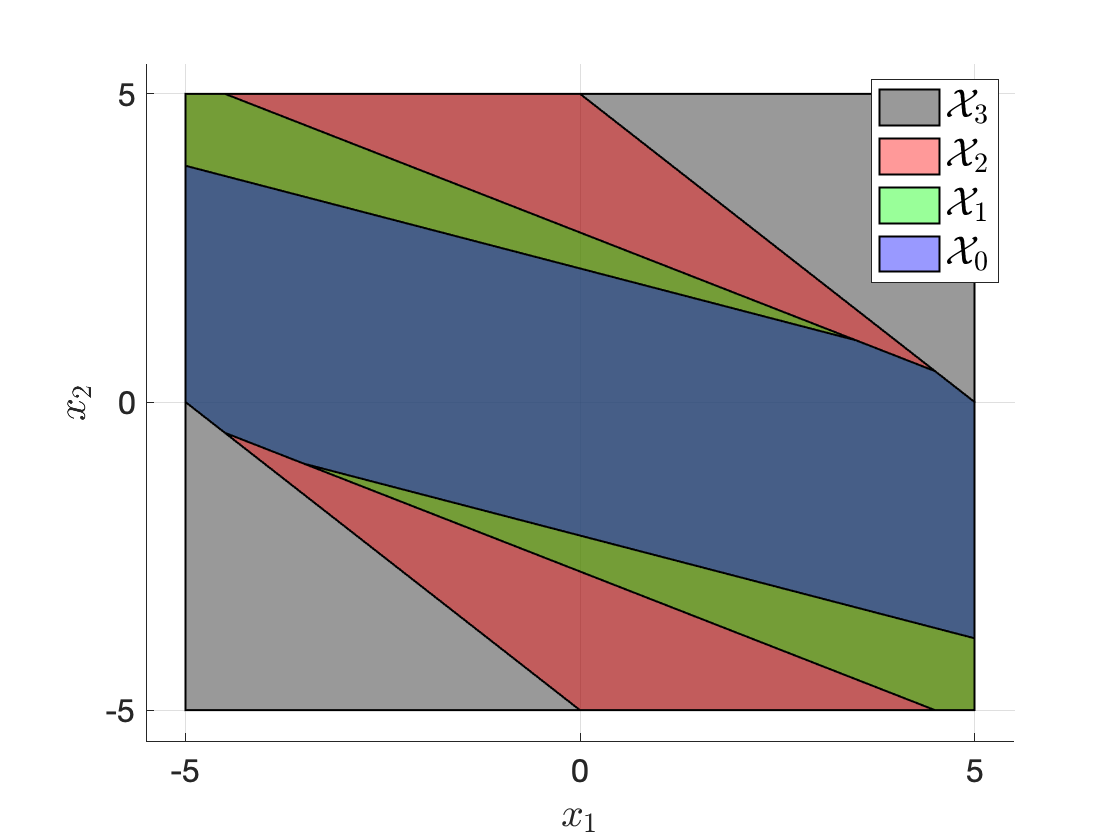
\includegraphics[width=0.6\linewidth]{images/double_integrator_feaset_1} 

}

\caption{Feasible sets of the double integrator receding horizon controller without terminal constraint.}\label{fig:double-integrator-feasible-set-1}
\end{figure}

\textbf{Choice 2}. \(\mathcal{X}_f = \{(0,0)\}\) is the origin. Fig. \ref{fig:double-integrator-feasible-set-2} plots the feasible sets. Observe that in this case \(\mathcal{X}_3 \subset \mathcal{X}_2 \subset \mathcal{X}_1 \subset \mathcal{X}_0\). This is a nice case, because if RHC starts at \(x_0 \in \mathcal{X}_0\) that is feasible, in the next iteration we have \(x_1 \in \mathcal{X}_1 \subset \mathcal{X}_0\), which implies that \(x_1\) is guaranteed to remain feasible!

In fact, as we will soon show, in the first choice the RHC does suffer from infeasibility.

\begin{figure}

{\centering 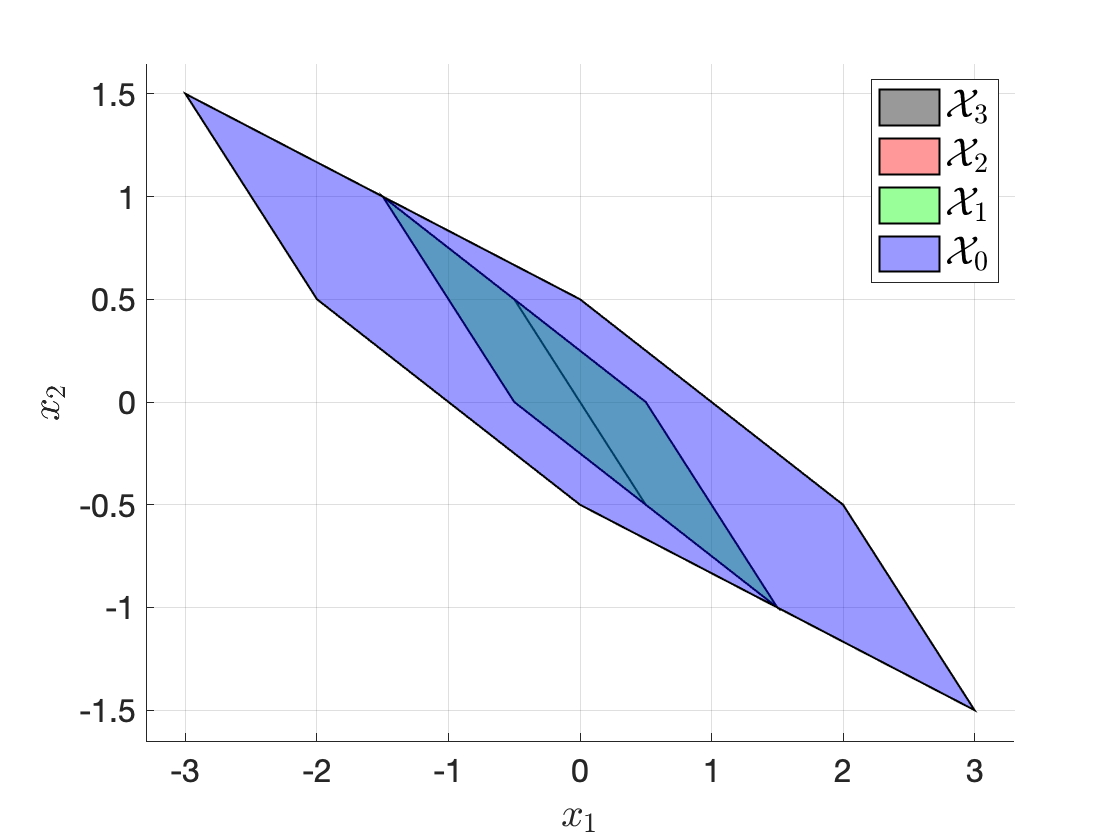
\includegraphics[width=0.6\linewidth]{images/double_integrator_feaset_2} 

}

\caption{Feasible sets of the double integrator receding horizon controller with terminal constraint.}\label{fig:double-integrator-feasible-set-2}
\end{figure}

The code for this example can be found \href{https://github.com/ComputationalRobotics/OptimalControlEstimation-Examples/blob/main/mpt_examples/double_integrator_feasible_sets.m}{here}.
\end{example}

\textbf{Algorithm}. Above all, problem \eqref{eq:linear-mpc-subroutine} is a convex optimization problem that we know how to solve efficiently (you have solved such convex optimization problems in Exercise \ref{exr:lqrconstraints}).

Let \(u^\star(0),\dots,u^\star(N-1)\) be the optimal solution of problem \eqref{eq:linear-mpc-subroutine} when it is feasible, the RHS framework will only apply the first control \(u^\star(0)\) to the system, and hence the closed-loop system is
\begin{equation}
x_{t+1} = A x_t + u^\star_{x_t}(0) = f_{\mathrm{cl}}(x_t),
\label{eq:mpc-closed-loop}
\end{equation}
where I have used \(u^\star_{x_t}(0)\) to make it explicit that the control is the first optimal control of solving \eqref{eq:linear-mpc-subroutine} with an initial state \(x_t\). The following algorithm summarizes the receding horizon control algorithm.

\begin{center}\rule{0.5\linewidth}{0.5pt}\end{center}

\textbf{Algorithm}: Online Receding Horizon Control

\begin{center}\rule{0.5\linewidth}{0.5pt}\end{center}

\textbf{Input:} State \(x_t\) at time \(t\)

\textbf{Output:} Control \(u^\star_{x_t}(0)\)

\begin{enumerate}
\def\labelenumi{\arabic{enumi}.}
\tightlist
\item
  Solve problem \eqref{eq:linear-mpc-subroutine} to get the optimal controls \(u^\star(0), \dots, u^\star(N-1)\)
\item
  \textbf{if} the problem is infeasible, \textbf{then} stop
\item
  \textbf{else} \textbf{return} \(u^\star_{x_t}(0) = u^\star(0)\)
\end{enumerate}

\begin{center}\rule{0.5\linewidth}{0.5pt}\end{center}

\textbf{RHC main questions}. Two main questions arise regarding the RHC controller.

\begin{enumerate}
\def\labelenumi{\arabic{enumi}.}
\item
  \textbf{Persistent feasibility}. If the RHC algorithm starts at a state \(x_0\) for which the convex optimization \eqref{eq:linear-mpc-subroutine} is feasible, i.e., \(x_0 \in \mathcal{X}_0\), will the convex optimization \eqref{eq:linear-mpc-subroutine} remain feasible for all future time steps?
\item
  \textbf{Stability}. Assuming the convex optimization is always feasible. Will the closed-loop system \eqref{eq:mpc-closed-loop} (induced by the RHC controller) converge to the desired origin \(x=0\)?
\end{enumerate}

Let us use a couple of examples to illustrate that, in general, the answers to the above two questions are both NO.

\begin{example}[Receding Horizon Control for Double Integrator]
\protect\hypertarget{exm:double-integrator-mpc}{}\label{exm:double-integrator-mpc}

Consider the discrete-time double integrator dynamics
\[
x_{t+1} = \begin{bmatrix} 1 & 1 \\ 0 & 1 \end{bmatrix} x_t + \begin{bmatrix} 0 \\ 1 \end{bmatrix} u_t,
\]
subject to control constraint
\[
u \in \mathcal{U} = [-0.5,0.5],
\]
and state constraint
\[
x \in \mathcal{X} = [-5, 5] \times [-5, 5].
\]
In the RHS subproblem \eqref{eq:linear-mpc-subroutine}, we use \(N = 3\), \(p(x) = x^T P x\), \(q(x,u) = x^T Q x + u^T R u\) with \(P = Q = I\), \(R=10\), and \(\mathcal{X}_f = \mathbb{R}^2\) (i.e., there is not terminal constraint). The subproblem is implemented using CVX in Matlab.

Fig. \ref{fig:double-integrator-mpc-two-initial-states} shows the state trajectory of executing RHC starting at \(x_0 = [-4.5;2]\) and \(x_0 = [-4.5;3]\), respectively.

We can see that when the initial state is \(x_0 = [-4.5;2]\), the trajectory successfully converges to the origin (the blue line). However, when the initial state is \(x_0 = [-4.5;3]\), RHC fails in the third iteration because the subproblem becomes infeasible (the red line).

You can find code for this example \href{https://github.com/ComputationalRobotics/OptimalControlEstimation-Examples/blob/main/double_integrator_mpc/double_integrator_mpc.m}{here}.

\begin{figure}

{\centering 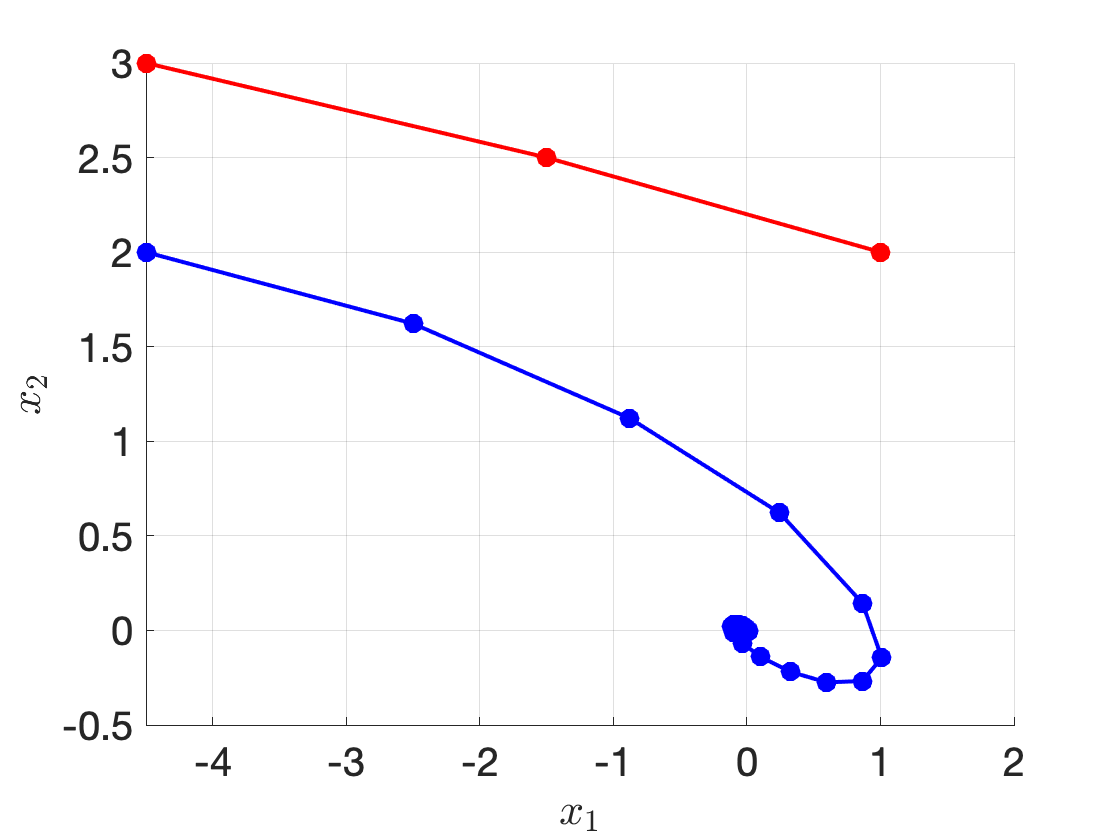
\includegraphics[width=0.7\linewidth]{images/double_integrator_mpc_two_initial_states} 

}

\caption{Receding horizon control for the double integrator with two initial states.}\label{fig:double-integrator-mpc-two-initial-states}
\end{figure}

\end{example}

We now show another example, adapted from \citep{borrelli17book-mpc} where the design of \(N\), \(p(x)\) and \(q(x,u)\) affects the closed-loop performance.

\begin{example}[RHC Performance Affected by Parameters]
\protect\hypertarget{exm:mpc-linear-design-choice}{}\label{exm:mpc-linear-design-choice}

Consider the system
\[
x_{t+1} = \begin{bmatrix}
2 & 1 \\ 0 & 0.5
\end{bmatrix} x_t + \begin{bmatrix} 1 \\ 0 \end{bmatrix} u_t,
\]
with control constraint
\[
u \in \mathcal{U} = [-1,1],
\]
and state constraint
\[
x \in \mathcal{X} = [-10,10] \times [-10,10].
\]

In the RHC problem \eqref{eq:linear-mpc-subroutine}, we choose \(p(x) = x^T P x\), \(q(x,u) = x^T Q x + u^T R u\). We fix \(P=0\), \(Q = I\), and \(\mathcal{X}_f = \mathbb{R}^2\), but vary \(N\) and \(R\):

\begin{itemize}
\item
  Setting 1: \(N=2\), \(R = 10\);
\item
  Setting 2: \(N=3\), \(R = 2\);
\item
  Setting 3: \(N=4\), \(R=1\).
\end{itemize}

Fig. \ref{fig:mpc-linear-effect-parameters} shows the closed-loop trajectories of three different settings. As we can see, the closed-loop performance depends on the parameters in a very complicated manner.

\begin{figure}

{\centering 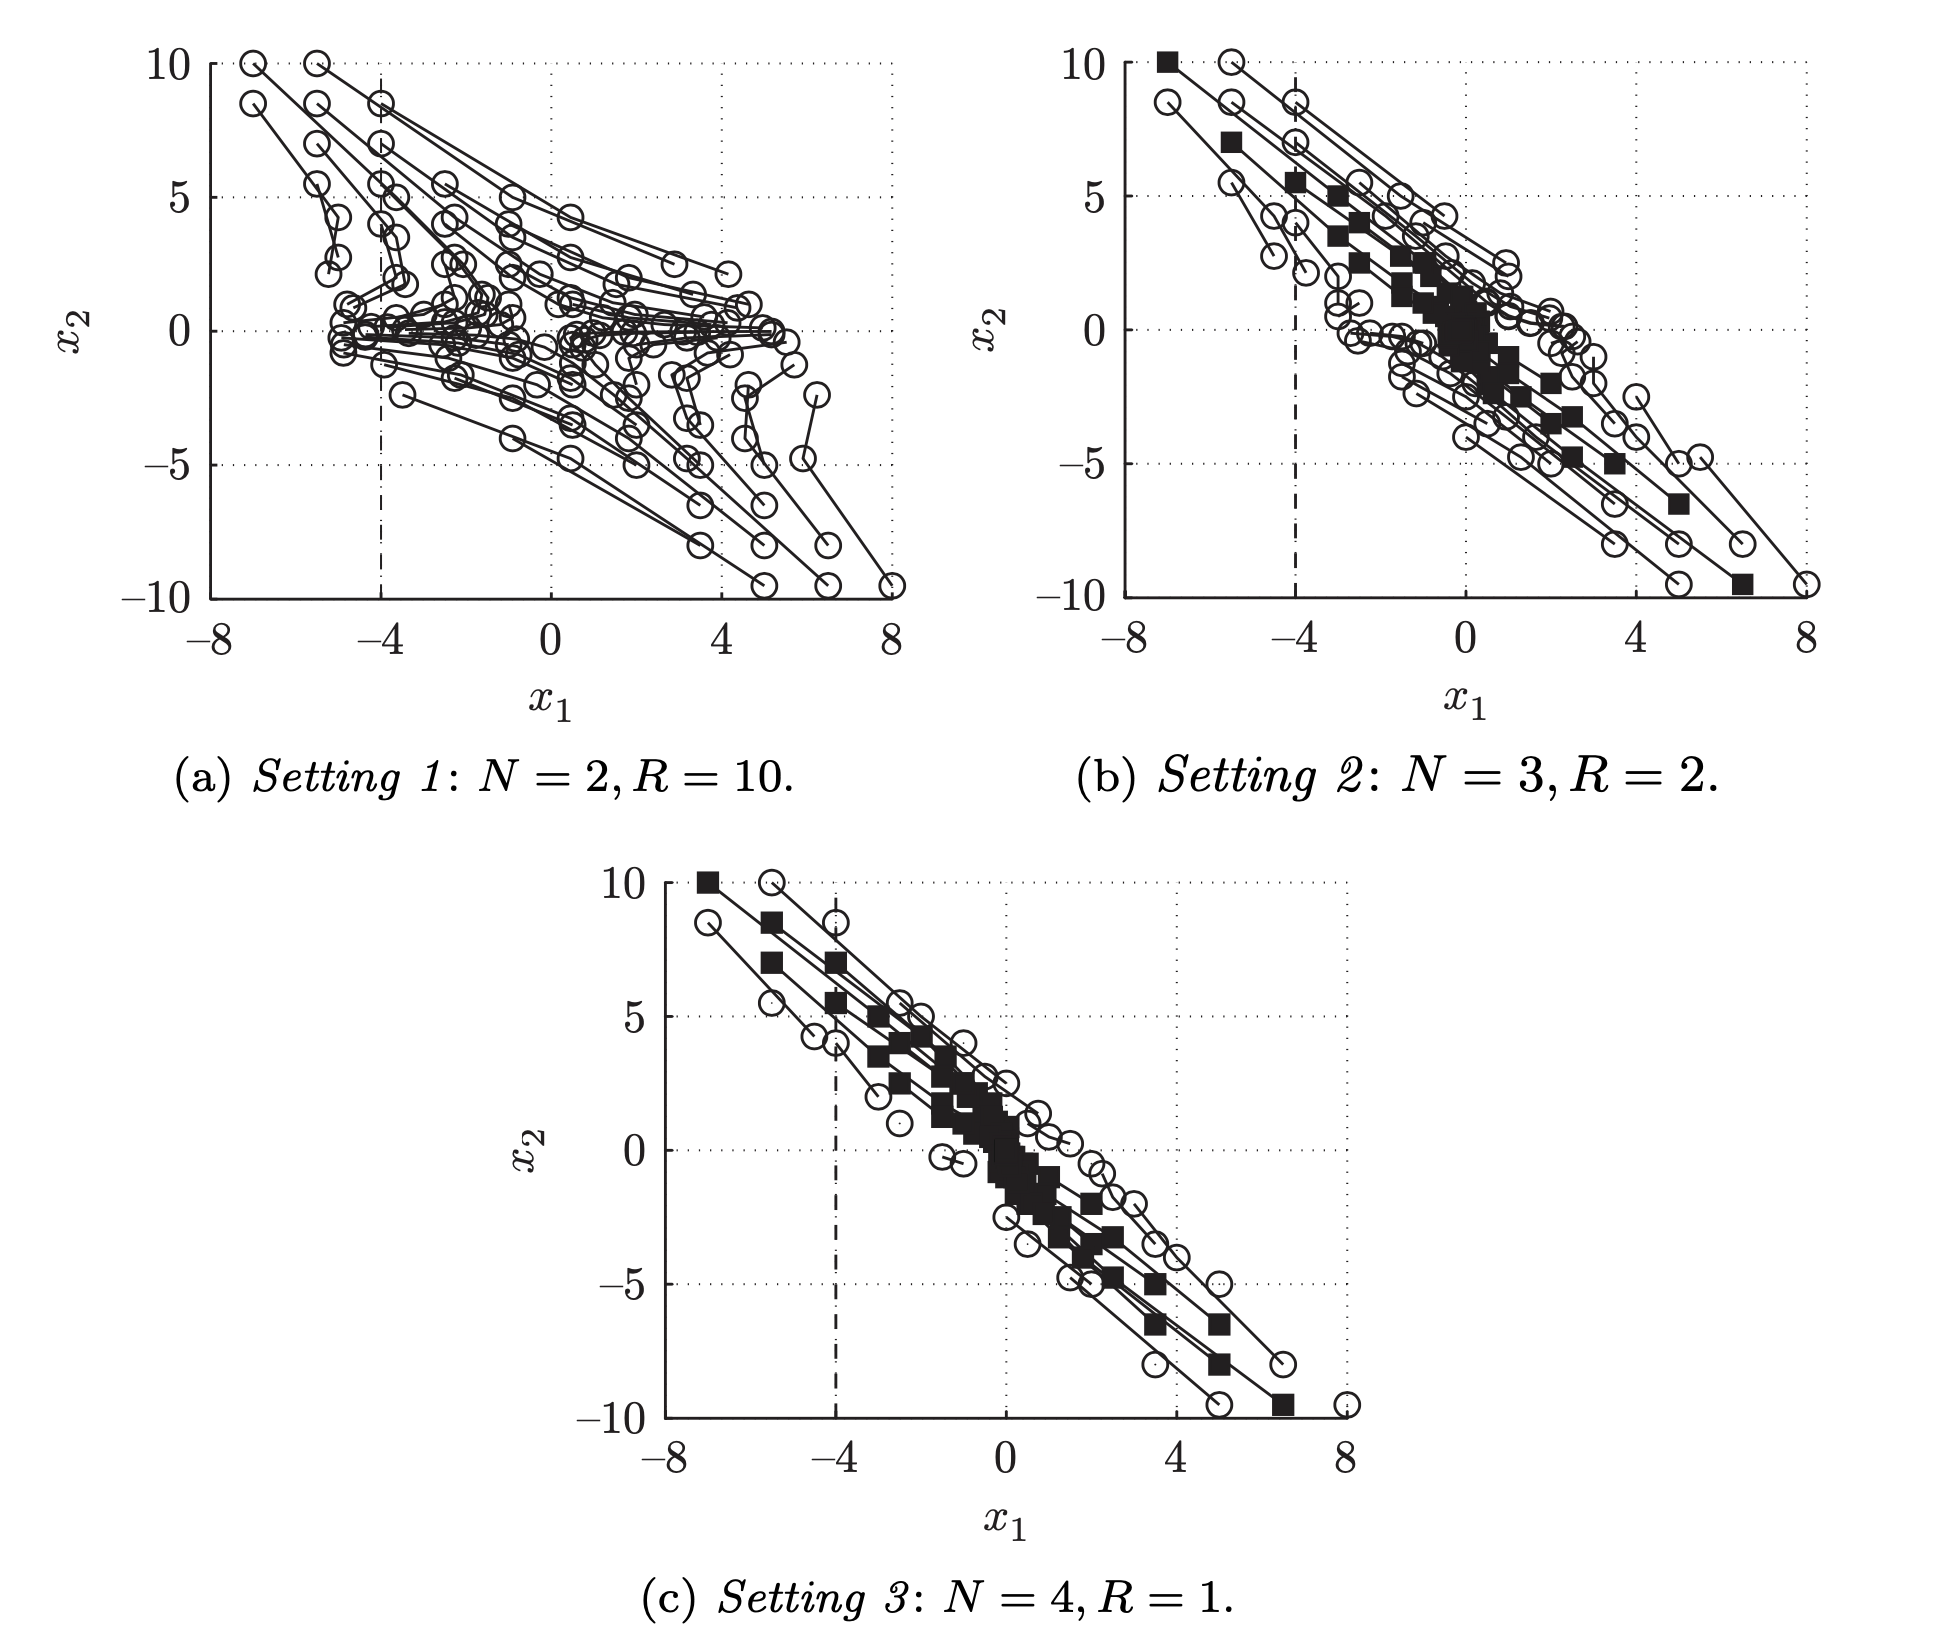
\includegraphics[width=0.8\linewidth]{images/mpc_linear_effect_parameter} 

}

\caption{Closed-loop trajectories for different settings of horizon N and weight R. Boxes (circles) are initial points leading to feasible (infeasible) closed-loop trajectories.}\label{fig:mpc-linear-effect-parameters}
\end{figure}

\end{example}

\hypertarget{persistent-feasibility}{%
\subsection{Persistent Feasibility}\label{persistent-feasibility}}

Under what conditions can we guarantee the RHC subproblem \eqref{eq:linear-mpc-subroutine} is always feasible?

Intuitively, we will show that, by designing the terminal constraint set \(\mathcal{X}_f\), we can guarantee the configuration of the feasible sets will look like choice 2 in Example \ref{exm:compute-calXi-double-integrator}.

There are various sets here of interest for answering this question.

\begin{itemize}
\item
  \(\mathcal{C}_{\infty}\): The maximal control invariant set \(\mathcal{C}_{\infty}\) is only affected by the system dynamics \eqref{eq:mpc-linear-system} and the constraint sets \(\mathcal{X} \times \mathcal{U}\). It is the largest set over which we can expect \emph{any} controller to work, because otherwise the system trajectory will blow up.
\item
  \(\mathcal{X}_0\): The set of states at which the RHC subproblem \eqref{eq:linear-mpc-subroutine} is feasible. The set \(\mathcal{X}_0\) depends on the system dynamics, the constraint sets \(\mathcal{X} \times \mathcal{U}\), as well as the RHC horizon \(N\) and the terminal constraint set \(\mathcal{X}_f\). It is worth noting that it does not depend on the objective function in \eqref{eq:linear-mpc-subroutine} (i.e., \(P,Q,R\)).
\item
  \(\mathcal{O}_{\infty}\): The maximal positive invariant set for the closed-loop system \eqref{eq:mpc-closed-loop} induced by the RHC control law. This depends on the RHC controller and hence it depends on the system dynamics, the constraint set \(\mathcal{X} \times \mathcal{U}\), \(N\), \(\mathcal{X}_f\) and the objective function of \eqref{eq:linear-mpc-subroutine} \(P,Q,R\).
\end{itemize}

A few relationships between these sets are easy to observe.

\begin{itemize}
\item
  \(\mathcal{O}_{\infty} \subseteq \mathcal{X}_0\). Any state \(x \in \mathcal{O}_{\infty}\) needs to stay in \(\mathcal{O}_{\infty}\) for all future time steps. Thus, the subproblem \eqref{eq:linear-mpc-subroutine} must be feasible for any \(x \in \mathcal{O}_{\infty}\), otherwise the closed-loop system \eqref{eq:mpc-closed-loop} is not even well defined.
\item
  \(\mathcal{O}_{\infty} \subseteq \mathcal{C}_{\infty}\). The set \(\mathcal{O}_{\infty}\) is control invariant because there exists a controller (specifically, the RHC controller) that makes it positive invariant. Therefore, \(\mathcal{O}_{\infty}\) must belong to the maximal control invariant set \(\mathcal{C}_{\infty}\).
\end{itemize}

We can now state necessary and sufficient conditions guaranteeing persistent feasibility.

\begin{lemma}[Sufficient and Necessary Condition for Persistent Feasibility]
\protect\hypertarget{lem:sufficient-necessary-feasibility}{}\label{lem:sufficient-necessary-feasibility}The RHC subproblem \eqref{eq:linear-mpc-subroutine} is persistently feasible if and only if \(\mathcal{X}_0 = \mathcal{O}_{\infty}\).
\end{lemma}

\begin{proof}
We have already argued that \(\mathcal{O}_{\infty} \subseteq \mathcal{X}_0\). It remains to show \(\mathcal{X}_0 \subseteq \mathcal{O}_{\infty}\). By definition, \(\mathcal{X}_0\) is persistently feasible implies that
\[
x \in \mathcal{X}_0 \Longrightarrow f_{\mathrm{cl}}^t(x) \in \mathcal{X}_0, \forall t
\]
where \(f_{\mathrm{cl}}^t\) means applying the closed-loop dynamics \(f_{\mathrm{cl}}\) in \eqref{eq:mpc-closed-loop} \(t\) times. This shows that \(\mathcal{X}_0\) is a positive invariant set for the closed-loop system, and hence \(\mathcal{X}_0 \subseteq \mathcal{O}_{\infty}\).
\end{proof}

We argued that \(\mathcal{X}_0\) does not depend on the RHC parameters \(P,Q,R\) but \(\mathcal{O}_{\infty}\) does. Therefore, in general only some \(P,Q,R\) are allowed for persistent feasibility to hold. Due to the complicated relationship between \(P,Q,R\) and \(\mathcal{O}_{\infty}\), it is generally difficult to design \(P,Q,R\) such that RHC has persistent feasibility.

We now state a sufficient condition for persistent feasibility to hold.

\begin{lemma}[Sufficient Condition for Persistent Feasibility]
\protect\hypertarget{lem:sufficient-feasibility}{}\label{lem:sufficient-feasibility}Consider the RHC subproblem \eqref{eq:linear-mpc-subroutine} with \(N \geq 1\). If \(\mathcal{X}_1\) is a control invariant set for the linear system \eqref{eq:mpc-linear-system}, then the RHC controller is persistently feasible.
\end{lemma}

\begin{proof}
If \(\mathcal{X}_1\) is control invariant, then by definition \(\mathcal{X}_1 \subseteq \text{Pre}(\mathcal{X}_1)\). Since \(\mathcal{X}_1 \subseteq \mathcal{X}\), we have
\[
\mathcal{X}_1 \subseteq \text{Pre}(\mathcal{X}_1) \cap \mathcal{X} = \mathcal{X}_0.
\]
where the last equality in the equation above is due to \eqref{eq:mpc-feasible-set-recursion}.
Now pick any \(x_0 \in \mathcal{X}_0\), the set of controls that make \(x_0\) feasible is denoted as
\[
U = \{ u(0),\dots,u(N-1) \mid x(0)=x_0, x(k) \in \mathcal{X},k=0,\dots,N-1,x(N) \in \mathcal{X}_f \}.
\]
The RHC will pick some control sequence from \(U\), say \(\hat{u}(0),\dots,\hat{u}(N-1)\) and apply the first control \(\hat{u}(0)\) to the system, which will bring the system to a new state
\[
x_1 = A x_0 + B \hat{u}(0).
\]
Observe that \(x_1 \in \mathcal{X}_1\) by definition. Since \(\mathcal{X}_1 \subseteq \mathcal{X}_0\), we have \(x_1 \in \mathcal{X}_0\). This proves that the RHC is persistently feasible, i.e., starting with any \(x_0 \in \mathcal{X}_0\), the RHC subproblem \eqref{eq:linear-mpc-subroutine} is always feasible.
\end{proof}

Lemma \ref{lem:sufficient-feasibility} states that if \(\mathcal{X}_1\) is control invariant, then the RHC subproblem is persistently feasible. An immediate result of this Lemma is that when \(N=1\), then \(\mathcal{X}_1 = \mathcal{X}_f\). Therefore, if we choose the terminal constraint set \(\mathcal{X}_f\) to be control invariant, then RHC is has persistent feasibility.

The next theorem states that when \(N \geq 1\), as long as we choose the terminal constraint set \(\mathcal{X}_f\) to be control invariant, then persistent feasibility also holds.

\begin{theorem}[Control Invariant Terminal Constraint Set Guarantees Persistent Feasibility]
\protect\hypertarget{thm:sufficient-feasibility-terminal}{}\label{thm:sufficient-feasibility-terminal}Consider the RHC subproblem \eqref{eq:linear-mpc-subroutine} with \(N \geq 1\). If \(\mathcal{X}_f\) is a control invariant set for the linear system \eqref{eq:mpc-linear-system}, then the RHC controller is persistently feasible.
\end{theorem}

\begin{proof}
We will prove that \(\mathcal{X}_f\) being control invariant implies
\[
\mathcal{X}_{N-1}, \mathcal{X}_{N-2},\dots,\mathcal{X}_1
\]
are all control invariant, and then by Lemma \ref{lem:sufficient-feasibility}, we can guarantee persistent feasibility. Fig. \ref{fig:mpc-nested-control-invariant-set} shows the nested control invariant sets when \(\mathcal{X}_f\) is control invariant.

\begin{figure}

{\centering 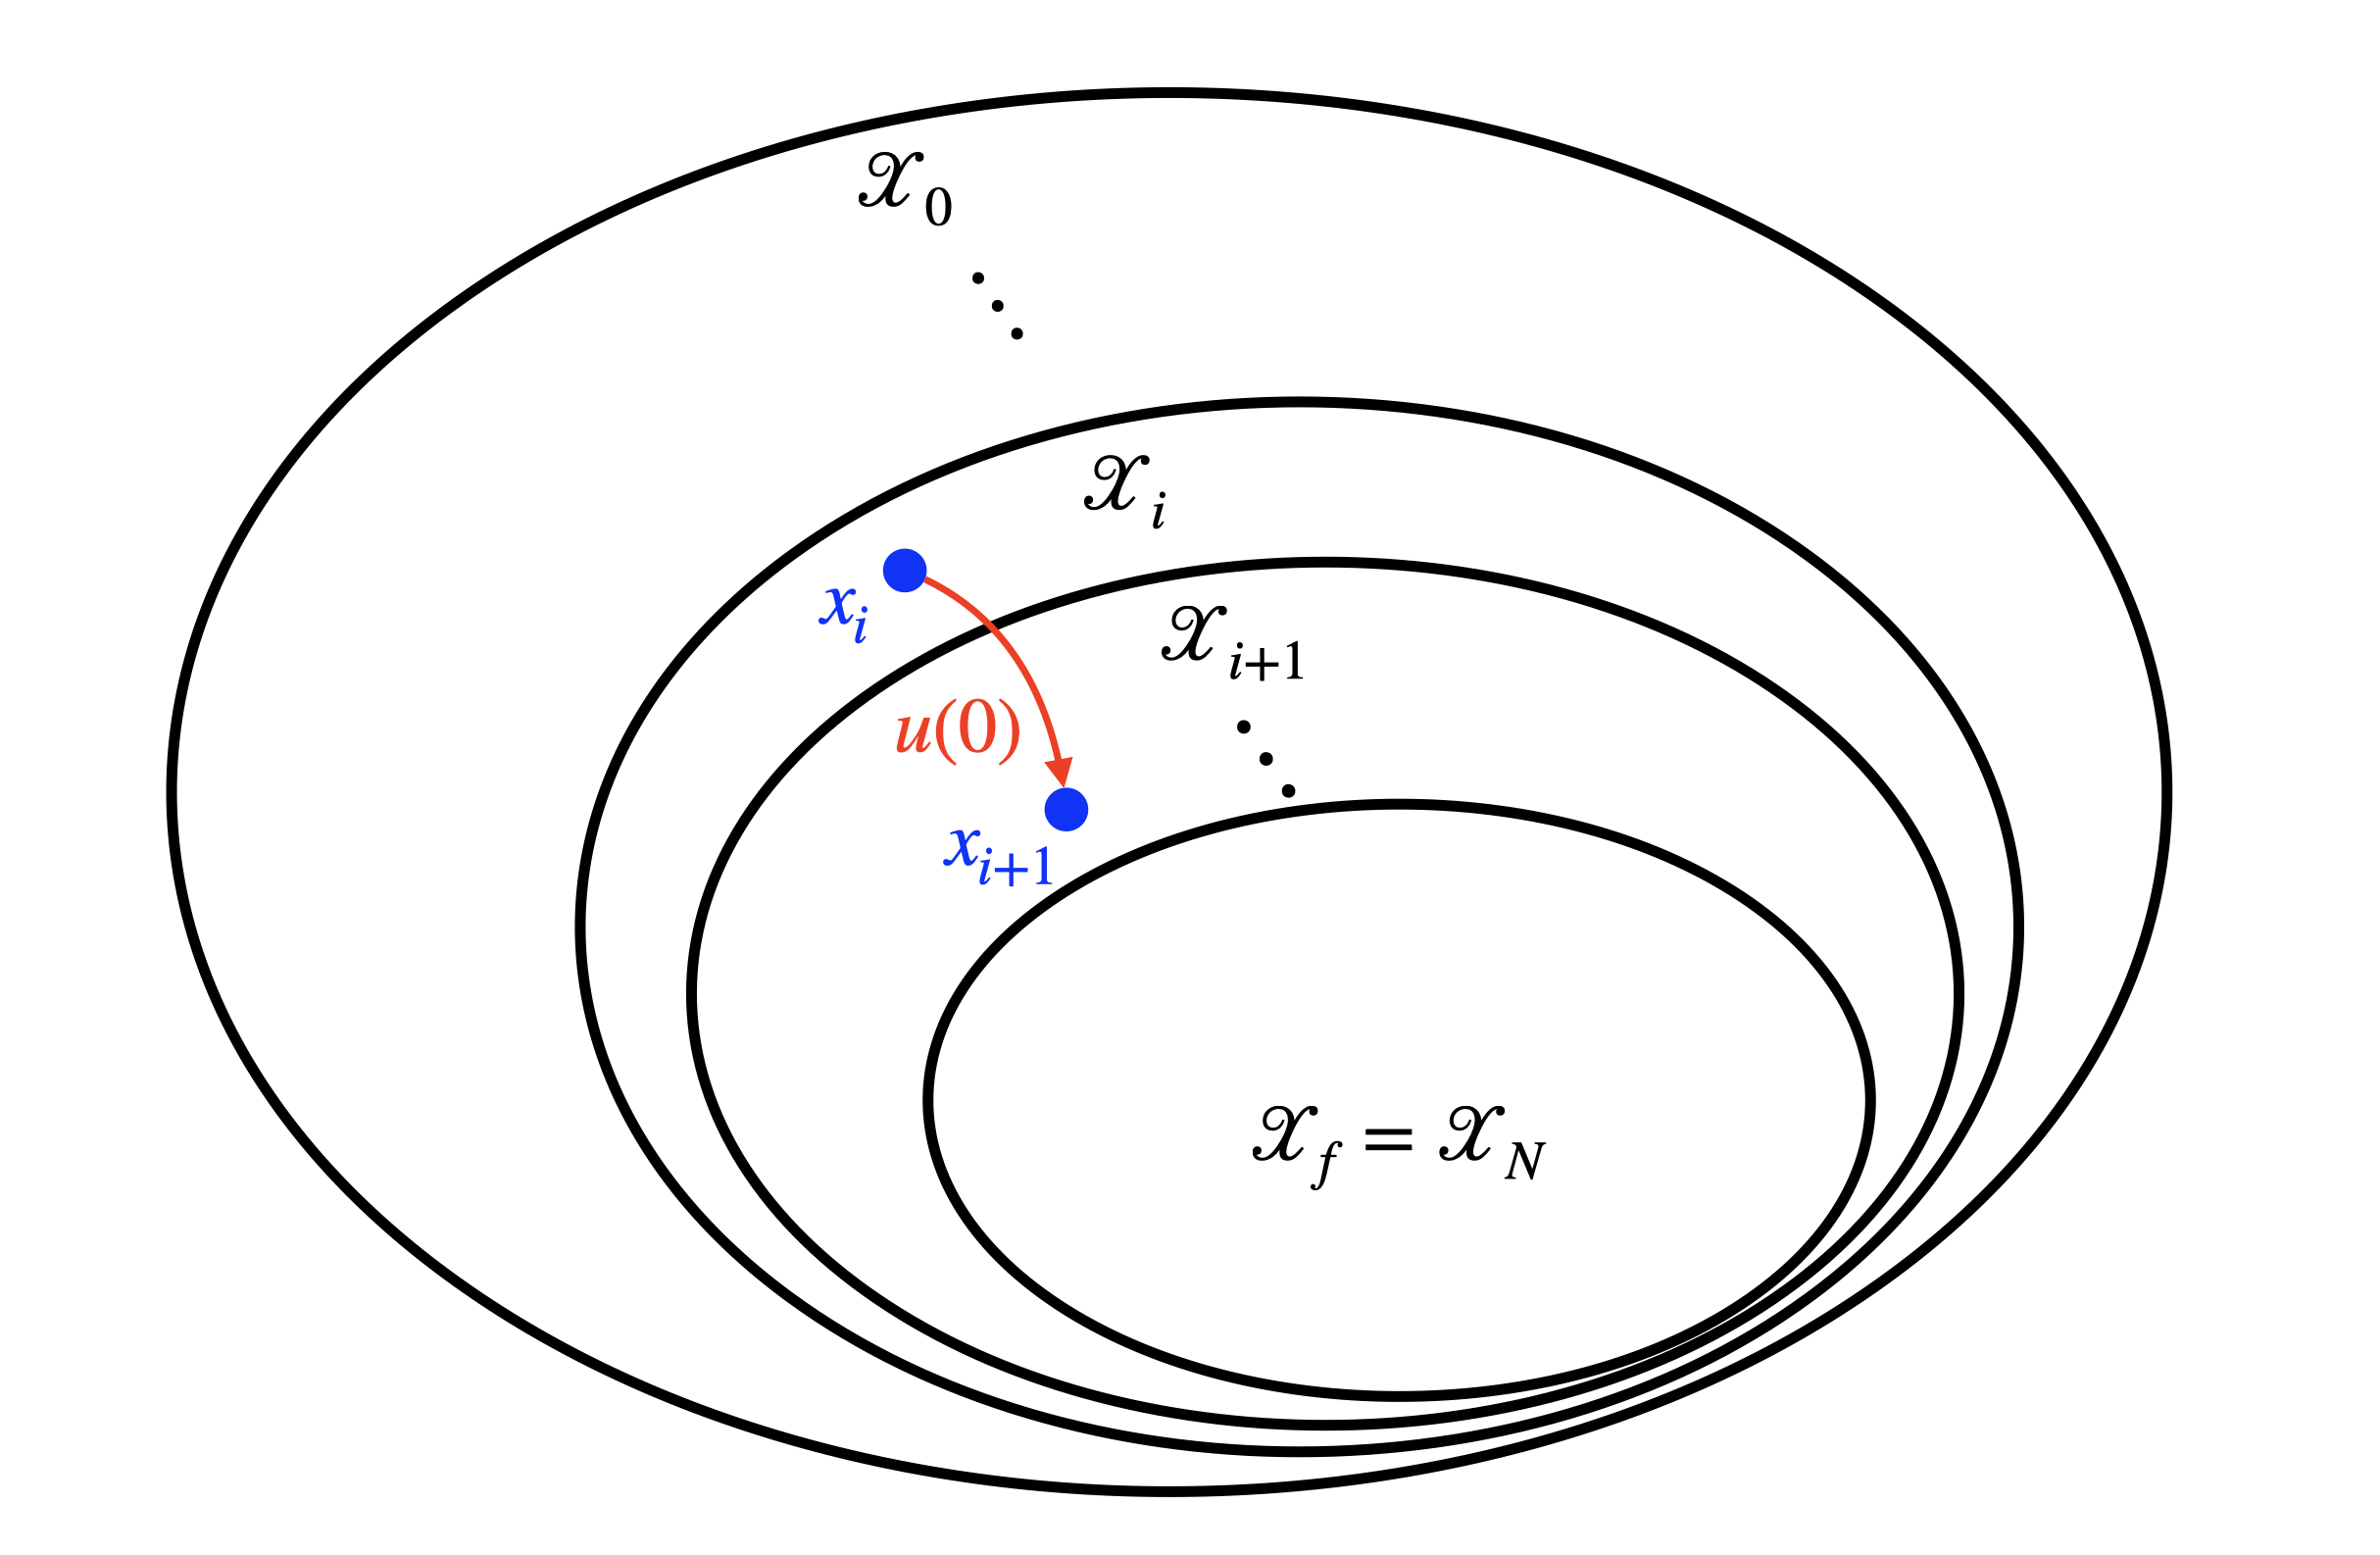
\includegraphics[width=0.8\linewidth]{images/mpc_nested_control_invariant_set} 

}

\caption{Nested control invariant sets.}\label{fig:mpc-nested-control-invariant-set}
\end{figure}

It suffices to show \(\mathcal{X}_{i+1}\) being control invariant leads to \(\mathcal{X}_i\) being control invariant. First, by \(\mathcal{X}_{i+1}\) control invariant, we have \(\mathcal{X}_{i+1} \subseteq \text{Pre}(\mathcal{X}_i) \cap \mathcal{X} = \mathcal{X}_i\). Now pick any \(x_{i} \in \mathcal{X}_{i}\), for any feasible \(\hat{u}(0),\dots,\hat{u}(N-1)\), applying the first control \(\hat{u}(0)\) brings the system to a new state
\[
x_{i+1} = A x_i + B \hat{u}(0) \in \mathcal{X}_{i+1} \subseteq \mathcal{X}_i.
\]
This shows \(\mathcal{X}_i\) is control invariant.
\end{proof}

Persistent feasibility does not guarantee the closed-loop system will converge to the origin. In fact, from Theorem \ref{thm:sufficient-feasibility-terminal}, it is clear that if the system starts at \(x_0 \in \mathcal{X}_0\), then we can only guarantee \(x_t \in \mathcal{X}_1\) for all \(t \geq 0\).

\hypertarget{mpc-stability}{%
\subsection{Stability}\label{mpc-stability}}

We now answer the question of how can we guarantee the RHC controller will drive the system to the desired origin.

\begin{theorem}[Sufficient Condition for Stability]
\protect\hypertarget{thm:mpc-stability}{}\label{thm:mpc-stability}Consider the linear system \eqref{eq:mpc-linear-system}, and the RHC algorithm \eqref{eq:linear-mpc-subroutine}. Assume that

\begin{enumerate}
\def\labelenumi{\arabic{enumi}.}
\item
  The stage cost \(q(x,u)\) and terminal cost \(p(x)\) are continuous and positive definite functions.
\item
  The sets \(\mathcal{X}\), \(\mathcal{X}_f\) and \(\mathcal{U}\) contain the origin in their interior and are closed.
\item
  \(\mathcal{X}_f \subseteq \mathcal{X}\) is control invariant.
\item
  For any \(x \in \mathcal{X}_f\), the following inequality holds
  \begin{equation}
  \min_{u \in \mathcal{U}, A x + Bu \in \mathcal{X}_f} \left( - p(x) + q(x,u) + p(Ax + Bu) \right) \leq 0.
  \label{eq:mpc-stability-lyapunov}
  \end{equation}
\end{enumerate}

Then, the origin of the closed-loop system \eqref{eq:mpc-closed-loop} is asymptotically stable with domain of attraction \(\mathcal{X}_0\). In words, for any \(x_0 \in \mathcal{X}_0\), if the closed-loop system \eqref{eq:mpc-closed-loop} starts at \(x_0\), then the system trajectory converges to the origin as \(t\) tends to infinity.
\end{theorem}

Let us interpret Theorem \ref{thm:mpc-stability} before proving it. It should be clear that the first three assumptions are easy to satisfy. For example, if we choose \(p(x) = x^T P x\) and \(q(x,u) = x^T Q x + u^T R u\) with \(P, Q, R \succ 0\), then assumption 1 is satisfied. Usually \(\mathcal{X}\) and \(\mathcal{U}\) are both polyhedral sets containing the origin in the interior, so assumption 2 also holds naturally. Finding a control invariant set \(\mathcal{X}_f\) is not a trivial task but there exists numerical algorithms for this task (e.g., using the algorithms introduced in Section \ref{mpc-compute-control-invariant-set}). After we find a control invariant \(\mathcal{X}_f\), by Theorem \ref{thm:sufficient-feasibility-terminal}, we know persistent feasibility will hold.

We now prove the theorem by showing that Assumption 4 guarantees stability. Before we show the proof, we need the concept of a \emph{Lyapunov function}. Below we introduce Lyapunov function for a discrete-time dynamical system, but we will study more details of Lyapunov function for continuous-time dynamical systems in Chapter \ref{stability}.

\begin{lemma}[Discrete-time Lyapunov Function]
\protect\hypertarget{lem:lyapunov-stability-discrete-time}{}\label{lem:lyapunov-stability-discrete-time}Consider the discrete-time autonomous system \eqref{eq:mpc-autonomous-system}, restated below for convenience:
\[
x_{t+1} = f_a(x_t),
\]
and assume \(x=0\) is an equilibrium point of the system, i.e., \(0 = f_a (0)\) (if the system starts at the origin, it stays at the origin). Let \(\Omega \subset \mathbb{R}^n\) be a closed and bounded set containing the origin.
If there exists a function \(V: \mathbb{R}^n \rightarrow \mathbb{R}\) that is (a) continuous at the origin, (b) finite for every \(x \in \Omega\), and (c) satisfies

\begin{enumerate}
\def\labelenumi{\arabic{enumi}.}
\item
  \(V\) is positive definite: \(V(0) = 0\) and \(V(x) > 0,\forall x \in \Omega \backslash \{ 0\}\),
\item
  \(V(x_{t+1}) - V(x_t) \leq - \alpha(x_t) < 0\) for any \(x_t \in \Omega \backslash \{ 0\}\),
\end{enumerate}

where \(\alpha: \mathbb{R}^n \rightarrow \mathbb{R}\) is a continuous positive definite function. Then \(x=0\) is asymptotically stable in \(\Omega\), i.e, if the system starts within \(\Omega\), then its trajectory tends to \(0\) as \(t \rightarrow \infty\).

A function \(V\) satisfying the conditions above is called a Lyapunov function for the system.
\end{lemma}

One can think of the Lyapunov function \(V\) as an energy function for the system \eqref{eq:mpc-autonomous-system} that maps a system state to a single scalar. Condition 1 in Lemma \ref{lem:lyapunov-stability-discrete-time} states that \(V\) (the energy function) is strictly positive except at the origin. Condition 2 in Lemma \ref{lem:lyapunov-stability-discrete-time} states that, the system energy \(V\) is strictly decreasing along any system trajectory. Therefore, we conclude that \(V\) must converge to \(V=0\), and hence any state trajectory must converge to the origin.

We will now use Lemma \ref{lem:lyapunov-stability-discrete-time} to prove RHC stability under Theorem \ref{thm:mpc-stability}.

\begin{proof}
Our goal is to prove that the optimal cost of the RHC problem \eqref{eq:linear-mpc-subroutine}, \(J_t^\star(x_t)\), is a Lyapunov function for the closed-loop system \eqref{eq:mpc-closed-loop} on the domain \(\mathcal{X}_0\). Then using Lemma \ref{lem:lyapunov-stability-discrete-time} we can conclude that the closed-loop system \eqref{eq:mpc-closed-loop} will converge to the origin.

\textbf{Positive definite}. Clearly, we have \(J_t^\star(0) = 0\) by the positive definiteness of \(p\) and \(q\) and the fact that \(x=0\) is an equilibrium point of the linear system \eqref{eq:mpc-linear-system}. For \(x_t \neq 0\), it is also clear that \(J_t^\star(x) > 0\). Therefore, \(J_t^\star(x)\) is positive definite on \(\mathcal{X}_0\).

\textbf{Strictly decrease}. It suffices to show \(J_1^\star(x_1) - J_0^\star(x_0) < 0\) because the constraints of the RHC problem \eqref{eq:linear-mpc-subroutine} is time-invariant. Pick any \(x_0 \in \mathcal{X}_0\), and let
\begin{equation}
\left( u^\star(0),u^\star(1),\dots,u^\star(N-1) \right)
\label{eq:mpc-stability-proof-control-1}
\end{equation}
be an optimal control trajectory to problem \eqref{eq:linear-mpc-subroutine}. Denote
\begin{equation}
\left( x_0,x(1),\dots,x(N) \right)
\label{eq:mpc-stability-proof-state-1}
\end{equation}
as the associated optimal state trajectory for problem \eqref{eq:linear-mpc-subroutine}. The RHC controller will apply \(u^\star(0)\) to the system, leading to the next state
\[
x_1 = x(1) = A x_0 + B u^\star(0).
\]
Then we will solve problem \eqref{eq:linear-mpc-subroutine} to get \(J^\star_1(x_1)\), and we want to show \(J^\star_1(x_1) < J^\star_0(x_0)\). Towards this, we will construct a feasible solution to \eqref{eq:linear-mpc-subroutine} starting at \(x_1\), and hence an upper bound on \(J^\star_1(x_1)\). Consider the control sequence
\begin{equation}
\left( u^\star(1),\dots,u^\star(N-1),v \right)
\label{eq:mpc-stability-proof-control-2}
\end{equation}
which is different from the control sequence in \eqref{eq:mpc-stability-proof-control-1} by removing \(u^\star(0)\) and appending \(v\). The corresponding state trajectory to \eqref{eq:mpc-stability-proof-control-2} is
\begin{equation}
\left( x_1 = x(1), x(2),\dots,x(N), Ax(N) + Bv \right)
\label{eq:mpc-stability-proof-state-2}
\end{equation}
which is different from the state trajectory in \eqref{eq:mpc-stability-proof-state-1} by removing \(x_0\) and appending \(A x(N) + Bv\). Since \(x(N) \in \mathcal{X}_f\) and \(\mathcal{X}_f\) is control invariant, there exists \(v\) such that \(Ax(N) + Bv \in \mathcal{X}_f\) and the corresponding control trajectory \eqref{eq:mpc-stability-proof-control-2} is feasible. Applying the control trajectory \eqref{eq:mpc-stability-proof-control-2} to the optimization problem \eqref{eq:linear-mpc-subroutine} will lead to the total cost
\[
J_1(x_1) = J_0^\star(x_0) - q(x_0,u^\star(0)) \underbrace{- p(x(N)) + q(x(N),v) + p(Ax(N) + Bv)}_{s(x(N),v)}.
\]
Now by assumption 4 in Theorem \ref{thm:mpc-stability}, we can choose \(v\) such that the sum \(s(x(N),v) \leq 0\). Consequently, we have
\[
J_1^\star(x_1) \leq J_1(x_1) \leq J_0^\star(x_0) - q(x_0,u^\star(0)),
\]
which leads to
\[
J_1^\star(x_1) - J_0^\star(x_0) \leq - q(x_0,u^\star(0)).
\]
Because the choice of \(x_0\) was arbitrary, we conclude that \(J_t^\star(x_t)\) strictly decreases along any system trajectory that starts within \(\mathcal{X}_0\).

\textbf{Continuity at the origin}. We will show that \(J_0^\star(x) \leq p(x)\) for any \(x \in \mathcal{X}_f\). With this argument, since \(p(x)\) is positive definite and continuous, then \(J_0^\star(x)\) must be continuous at the origin. We now prove \(J_0^\star(x) \leq p(x)\) for any \(x \in \mathcal{X}_f\). Since \(\mathcal{X}_f\) is control invariant, pick any \(x \in \mathcal{X}_f\), there exists a sequence of controls \((u(0),u(1),\dots,u(N-1))\) such that the state trajectory \((x(0)=x,x(1),\dots,x(N))\) stays in \(\mathcal{X}_f\). Such a control sequence lead to an upper bound on \(J^\star_0(x)\):
\[
J^\star_0(x(0)) \leq p(x(N)) + \sum_{i=0}^{N-1} q(x(i),u(i)) = p(x(0)) + \sum_{i=0}^{N-1} \left( q(x(i),u(i)) + p(x(i+1)) - p(x(i)) \right),
\]
since each \(x(i) \in \mathcal{X}_f\), according to Assumption 4, we can choose \(u(i)\) such that
\[
J^\star_0(x(0)) \leq p(x(0))
\]
for any \(x(0) \in \mathcal{X}_f\).

In conclusion, we have shown that \(J^\star_t(x_t)\) is a Lyapunov function, and by Lemma \ref{lem:lyapunov-stability-discrete-time}, the closed-loop system is asymptotically stable.
\end{proof}

A function \(p(x)\) that satisfies Assumption 4 in Theorem \ref{thm:mpc-stability} is typicalled known as a \emph{control Lyapunov function}.

Now two natural problems arise:

\begin{enumerate}
\def\labelenumi{\arabic{enumi}.}
\item
  Given \(p(x)\), how to verify if assumption 3 holds in Theorem \ref{thm:mpc-stability}?
\item
  How to synthesize a \(p(x)\) that satisfies assumption 3 in Theorem \ref{thm:mpc-stability}?
\end{enumerate}

Unfortunately, both problems are hard. To see this, suppose we are given a candidate function \(p(x) = x^T P x\) with \(P \succ 0\) that is clearly positive definite. Assume \(q(x,u) = x^T Q x + u^T R u\) with \(Q, R \succ 0\) and \(\mathcal{U}, \mathcal{X}_f\) are given polyhedral sets. Then verifying if \(p(x)\) satisifies Assumption 4 boils down to checking if
\[
\min_{u \in \mathcal{U}, Ax + Bu \in \mathcal{X}_f} x^T Q x + u^T R u + (Ax + Bu)^T P (Ax + Bu) - x^T P x
\]
is non-positive for any possible \(x \in \mathcal{X}_f\). Although for each possible \(x\), the above problem is a convex optimization problem, there are an infinite number of points in the set \(\mathcal{X}_f\) and enumerating over all points is a daunting task. We will see in Chapter \ref{stability} that convex relaxations, in particular \href{https://hankyang.seas.harvard.edu/Semidefinite/}{semidefinite relaxations}, can help us partially solve these hard problems.

\textbf{A simple control lyapunov function}. One can solve the infinite-horizon unconstrained LQR problem
\[
\min_{u_t} \sum_{t=0}^{\infty}x_t ^T Q x_t + u_t^T R u_t,
\]
for which the optimal cost-to-go is
\[
J_{\infty}(x) = x^T S x, 
\]
with \(S\) the solution to the algebraic Riccati equation \eqref{eq:algebraic-riccati}. Denote
\[
u_t = \Pi_{\mathcal{U}} (- K x_t)
\]
as the optimal controller (\(\Pi_{\mathcal{U}}\) is the projection of the controller to the feasible set \(\mathcal{U}\)), and use \(\mathcal{X}_f\) as the maximal positive invariant set of the closed-loop system
\[
x_{t+1} = A x_t + B u_t.
\]
Then \(J_{\infty}(x) = x^T S x\) is a control Lyapunov function over the set \(\mathcal{X}_f\).

\hypertarget{explicit-mpc}{%
\subsection{Explicit MPC}\label{explicit-mpc}}

See the original paper \citep{bemporad02automatica-explicit}, and check out Matlab's \href{https://www.mathworks.com/help/mpc/explicit-mpc-design.html}{explict MPC design}.

\hypertarget{policy-gradient}{%
\section{Policy Gradient}\label{policy-gradient}}

\hypertarget{continuous-time-optimal-control}{%
\chapter{Continuous-time Optimal Control}\label{continuous-time-optimal-control}}

So far we have been focusing on stochastic and discrete-time optimal control problems. In this Chapter, we will switch gear to deterministic and continuous-time optimal control (still with continuous state and action space).

The goal of a continuous-time introduction is threefold. (1) Real-world systems are natively continuous-time. (2) We will see the continuous-time analog of the Bellman principle of optimality in discrete-time (cf.~Theorem \ref{thm:bellmanoptimality}). (3) The continuous-time setup is more natural and popular for stability analysis to be introduced in Chapter \ref{stability}.

\hypertarget{the-basic-problem-1}{%
\section{The Basic Problem}\label{the-basic-problem-1}}

Consider a continuous-time dynamical system
\begin{equation}
\dot{x}(t) = f(x(t),u(t)),\ t \in [0,T], \quad x(0) = x_0,
\label{eq:ct-optimal-control-system}
\end{equation}
where

\begin{itemize}
\item
  \(x(t) \in \mathbb{R}^n\) is the state of the system,
\item
  \(u(t) \in \mathbb{U} \subseteq \mathbb{R}^m\) is the control we wish to design,
\item
  \(f: \mathbb{R}^{n} \times \mathbb{R}^m \rightarrow \mathbb{R}^n\) models the system dynamics, and
\item
  \(x_0 \in \mathbb{R}^n\) is the initial state of the system.
\end{itemize}

We assume the admissible control functions \(\{u(t) \mid u(t) \in \mathbb{U}, t\in [0,T] \}\), also called control trajectories, must be \emph{piecewise continuous}.\footnote{Even though we write \(dx_i(t)/dt\) in the system \eqref{eq:ct-optimal-control-system}, we allow \(x(t)\) to be only directionally differentiable at a finite number of points to account for the possible discontinuity of \(u(t)\).} For any control trajectory, we assume the system \eqref{eq:ct-optimal-control-system} has a unique solution \(\{x(t)\mid t \in [0,T] \}\), called the state trajectory.

We now state the continuous-time optimal control problem.

\begin{definition}[Continuous-time, Finite-horizon Optimal Control]
\protect\hypertarget{def:continuoustimeoptimalcontrol}{}\label{def:continuoustimeoptimalcontrol}Find the best admissible control trajectory \(\{u(t) \mid t \in [0,T] \}\) that minimizes the cost function
\begin{equation}
J(0,x_0) = \min_{u(t) \in \mathbb{U}} h(x(T)) + \int_0^T g(x(t),u(t)) dt,
\label{eq:ct-optimal-control-definition}
\end{equation}
subject to \eqref{eq:ct-optimal-control-system}, where the functions \(g\) and \(h\) are continuously differentiable with respect to \(x\), and \(g\) is continuous with respect to \(u\).
\end{definition}

The function \(J\) in \eqref{eq:ct-optimal-control-definition} is called the \emph{optimal cost-to-go}, or the \emph{optimal value function}. Notice that the optimal cost-to-go is a function of both the state \(x\) and the time \(t\), just as in the discrete-time case we used \(J_k\) with a subscript \(k\) to denote the optimal cost-to-go for the tail problem starting at timestep \(k\) (cf.~Theorem \ref{thm:dynamicprogramming}). Specifically, we should interpret
\[
J(t,x_0) = \min_{u(t) \in \mathbb{U}} h(x(T)) + \int_t^T g(x(\tau),u(\tau)) d\tau, \quad x(t) = x_0,
\]
as the optimal cost-to-go of the system starting from \(x_0\) at time \(t\) (i.e., the tail problem).
We assume \(J(0,x_0)\) is finite when \(x_0\) is in some set \(\mathcal{X}_0\).

\hypertarget{the-hamilton-jacobi-bellman-equation}{%
\section{The Hamilton-Jacobi-Bellman Equation}\label{the-hamilton-jacobi-bellman-equation}}

Recall that in discrete-time, the dynamic programming (DP) algorithm in Theorem \ref{thm:dynamicprogramming} states that the optimal cost-to-go has to satisfy a recursive equation \eqref{eq:dpbackwardrecursion}, i.e., the optimal cost-to-go at time \(k\) can be calculated by choosing the best action that minimizes the stage cost at time \(k\) plus the optimal cost-to-go at time \(k+1\). In the next, we will show a result of similar flavor to \eqref{eq:dpbackwardrecursion}, but in the form of a partial differential equation (PDE), known as the Hamilton-Jacobi-Bellman (HJB) equation.

Let us informally derive the HJB equation by applying the DP algorithm to a discrete-time approximation of the continuous-time optimal control problem. We divide the time horizon \([0,T]\) into \(N\) pieces of equal length \(\delta = T/N\), and denote
\[
x_k = x(k\delta), \quad u_k = u(k \delta), \quad k = 0,1,\dots,N.
\]
We then approximate the continuous-time dynamics \eqref{eq:ct-optimal-control-system} as
\[
x_{k+1} = x_k + \dot{x}_k \cdot \delta = x_k + f(x_k,u_k) \cdot \delta,
\]
and the cost function in \eqref{eq:ct-optimal-control-definition} as
\[
h(x_N) + \sum_{k=0}^{N-1} g(x_k, u_k)\cdot \delta.
\]
This problem now is in the form of a discrete-time, finite-horizon optimal control \ref{def:basicproblem}, for which we can apply dynamic programming.

Let us use \(\tilde{J}(t,x)\) (as opposed to \(J(t,x)\)) to denote the optimal cost-to-go at time \(t\) and state \(x\) for the discrete-time approximation. According to \eqref{eq:dpbackwardrecursion}, the DP backward recursion is
\begin{align}
\tilde{J}(N\delta,x) = h(x), \\
\tilde{J}(k\delta,x) = \min_{u \in \mathbb{U}} \left[ g(x,u)\cdot \delta + \tilde{J}((k+1)\delta,x + f(x,u)\cdot \delta)  \right], \quad k = N-1,\dots,0.
\label{eq:ct-optimal-control-discrete-approx-dp}
\end{align}
Suppose \(\tilde{J}(t,x)\) is differentiable, we can perform a Taylor-series expansion of \(\tilde{J}((k+1)\delta,x+f(x,u)\delta)\) in \eqref{eq:ct-optimal-control-discrete-approx-dp} as follows
\[
\tilde{J}((k+1)\delta,x+f(x,u)\delta) = \tilde{J}(k\delta,x) + \nabla_t \tilde{J} (k\delta,x) \cdot \delta + \nabla_x \tilde{J}(k\delta,x)^T f(x,u) \cdot \delta + o(\delta),
\]
where \(o(\delta)\) includes high-order terms that approach zero when \(\delta\) tends to zero, \(\nabla_t \tilde{J}\) and \(\nabla_x \tilde{J}\) (a column vector) denote the partial derivates of \(\tilde{J}\) with respect to \(t\) and \(x\), respectively. Plugging the first-order Taylor expansion into the DP recursion \eqref{eq:ct-optimal-control-discrete-approx-dp}, we obtain
\begin{equation}
\tilde{J}(k\delta,x) = \min_{u \in \mathbb{U}} \left[ g(x,u) \cdot \delta + \tilde{J}(k \delta,x) + \nabla_t \tilde{J}(k \delta,x) \delta + \nabla_x \tilde{J}(k\delta,x)^T f(x,u) \delta + o(\delta)  \right].
\label{eq:ct-optimal-control-discrete-approx-taylor}
\end{equation}
Cancelling \(\tilde{J}(k \delta,x)\) from both sides, dividing both sides by \(\delta\), and assuming \(\tilde{J}\) converges to \(J\) uniformly in time and state, i.e.,
\[
\lim_{\delta \rightarrow 0, k\delta = t} \tilde{J}(k\delta,x) = J(t,x), \quad \forall t,x,
\]
we obtain from \eqref{eq:ct-optimal-control-discrete-approx-taylor} the following partial differential equation
\begin{equation}
0 = \min_{u \in \mathbb{U}} \left[ g(x,u) + \nabla_t J(t,x) + \nabla_x J(t,x)^T f(x,u)  \right], \quad \forall t, x,
\label{eq:hjb-informal}
\end{equation}
with the boundary condition \(J(T,x) = h(x)\). Equation \eqref{eq:hjb-informal} is called the Hamilton-Jacobi-Bellman equation.

Our derivation above is informal, let us formally state the HJB equation.

\begin{theorem}[Hamilton-Jacobi-Bellman Equation as A Sufficient Condition for Optimality]
\protect\hypertarget{thm:hjbsufficient}{}\label{thm:hjbsufficient}Consider the optimal control problem \ref{def:continuoustimeoptimalcontrol} for system \eqref{eq:ct-optimal-control-system}. Suppose \(V(t,x)\) is a solution to the Hamilton-Jacobi-Bellman equation, i.e., \(V(t,x)\) is continuously differentiable and satisfies
\begin{align}
\label{eq:hjb-eqution-formal-1}
0 = \min_{u \in \mathbb{U}} \left[ g(x,u) + \nabla_t V(t,x) + \nabla_x V(t,x)^T f(x,u)\right], \quad \forall t,x, \\
V(T,x) = h(x), \quad \forall x.
\end{align}
Suppose \(\mu^\star(t,x)\) attains the minimum in \eqref{eq:hjb-eqution-formal-1} for all \(t\) and \(x\). Let \(\{x^\star(t) \mid t \in [0,T] \}\) be the state trajectory obtained from the given initial condition \(x(0)\) when the control trajectory \(u^\star(t) = \mu^\star(t,x^\star(t))\) is applied, i.e., \(x^\star(0) = x(0)\) and for any \(t \in [0,T]\), \(\dot{x}^\star(t) = f(x^\star(t), \mu^\star(t,x^\star(t)))\) and we assume this differential equation has a unique solution starting at any \((t,x)\) and that the control trajectory \(\{ \mu^\star(t,x^\star(t)) \mid t \in [0,T] \}\) is piecewise continuous as a function of \(t\).
Then \(V(t,x)\) is equal to the optimal cost-to-go \(J(t,x)\) for all \(t\) and \(x\). Moreover, the control trajectory \(u^\star(t)\) is optimal.
\end{theorem}

\begin{proof}
Let \(\{\hat{u}(t) \mid t \in [0,T] \}\) be any admissible control trajectory and let \(\hat{x}(t)\) be the resulting state trajectory. From the ``\(\min\)'' in \eqref{eq:hjb-eqution-formal-1}, we know
\[
0 \leq g(\hat{x},\hat{u}) + \nabla_t V(t,\hat{x}) + \nabla_x V(t,\hat{x})^T f(\hat{x},\hat{u}) = g(\hat{x},\hat{u}) + \frac{d}{dt} V(t,\hat{x}).
\]
Integrating the above inequality over \(t \in [0,T]\), we obtain
\[
0 \leq \left( \int_{0}^T g(\hat{x}(t),\hat{u}(t))dt \right) + V(T,\hat{x}(T)) - V(0,\hat{x}(0)).
\]
Using the terminal constraint \(V(T,x) = h(x)\) for any \(x\) and the initial condition \(\hat{x}(0) = x(0)\), we have
\[
V(0,x(0)) \leq h(\hat{x}(T)) + \int_{0}^T g(\hat{x}(t),\hat{u}(t)) dt.
\]
This shows that \(V(0,x(0))\) is a lower bound to the optimal cost-to-go, because any admissible control trajectory \(\hat{u}(t)\) leads to a cost no smaller than \(V(0,x(0))\).

It remains to show that \(V(0,x(0))\) is attainable. This is done by plugging the optimal control trajectory \(u^\star(t)\) and state trajectory \(x^\star(t)\) to the derivation above, leading to
\[
V(0,x(0)) = h(x^\star(T)) + \int_0^T g(x^\star(t),u^\star(t)) dt.
\]
This shows that \(V(0,x(0)) = J(0,x(0))\).

The argument above is generic and holds for any initial time \(t \in [0,T]\) and initial state \(x\). Therefore, \(V(t,x) = J(t,x)\) is the optimal cost-to-go.
\end{proof}

Theorem \ref{thm:hjbsufficient} effectively turns the optimal control problem \eqref{eq:ct-optimal-control-definition} into finding a solution for the partial differential equation \eqref{eq:hjb-eqution-formal-1}. Let us illustrate the theorem using a simple example.

\begin{example}[A Scalar System]
\protect\hypertarget{exm:hjbequationsimpleexample}{}\label{exm:hjbequationsimpleexample}Consider the following dynamical system
\[
\dot{x}(t) = u(t), \quad t \in [0,T]
\]
where \(x \in \mathbb{R}\) is the state, and \(u \in \mathbb{U} = [-1,1]\) is the control.

We are interested in the following optimal control problem
\[
\min_{u(t)} \frac{1}{2} \left( x(T) \right)^2,
\]
where the goal is to move the initial state as close as possible to the origin \(0\) at the terminal time \(T\).

There is a simple optimal controller for this scalar system. We move the state as quickly as possible to the origin \(0\), using maximum control, and then maintain the state at the origin using zero control. Formally, this is
\[
\mu^\star(t,x) = - \text{sgn}(x) = \begin{cases}
1 & \text{if } x < 0 \\
0 & \text{if } x = 0 \\
-1 & \text{if } x > 0
\end{cases}.
\]
With this controller, we know that if the system starts at \(x\) at time \(t\), the terminal state will satisfy
\[
\vert x(T) \vert = \begin{cases}
|x| - (T - t) & \text{if } T-t < |x|  \\
0 & \text{otherwise} 
\end{cases}.
\]
As a result, the optimal cost-to-go is
\begin{equation}
J(t,x) = \frac{1}{2} \left( \max\{0,  |x| - (T - t)\} \right)^2.
\label{eq:scalar-system-optimal-value}
\end{equation}

Let us verify if this function satisfies the HJB equation.

\textbf{Boundary condition}. Clearly,
\[
J(T,x) = \frac{1}{2}x^2
\]
satisfies the boundary condition.

\textbf{Differentiability}. When viewed as a function of \(t\), \(J(t,x)\) in \eqref{eq:scalar-system-optimal-value} can be plotted as in Fig. \ref{fig:scalar-system-optimal-J-t}. We can see that \(J(t,x)\) is differentiable in \(t\) and
\begin{equation}
\nabla_t J(t,x) = \max\{ 0, |x| - (T-t) \}.
\label{eq:scalar-system-partial-J-partial-t}
\end{equation}

\begin{figure}

{\centering 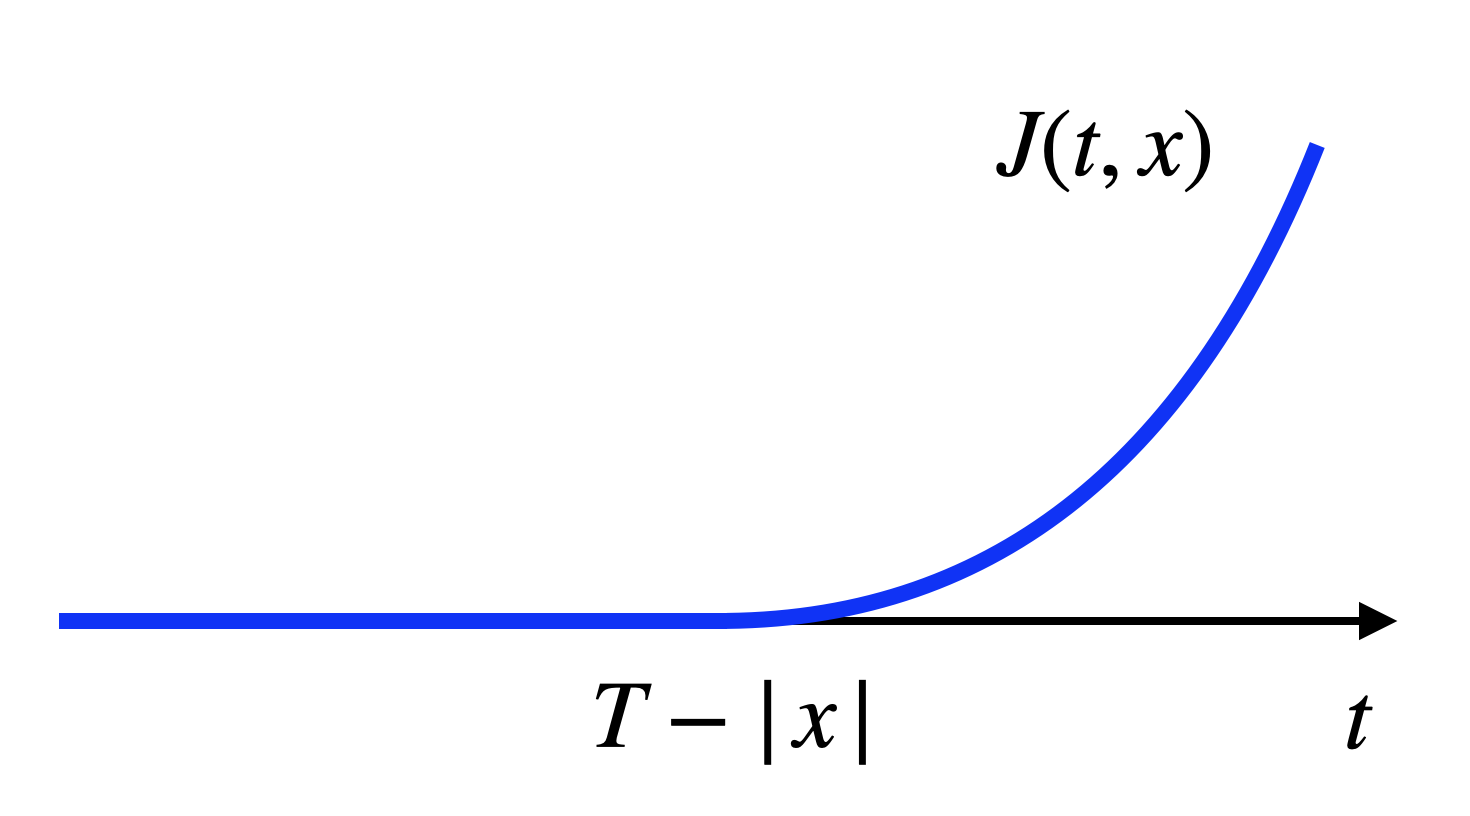
\includegraphics[width=0.5\linewidth]{images/scalar-system-optimal-J-t} 

}

\caption{Optimal cost-to-go as a function of time.}\label{fig:scalar-system-optimal-J-t}
\end{figure}

When viewed as a function of \(x\), \(J(t,x)\) can be plotted as in Fig. \ref{fig:scalar-system-optimal-J-x}. We can see \(J(t,x)\) is differentiable in \(x\) and
\begin{equation}
\nabla_x J(t,x) = \text{sgn}(x) \cdot \max\{ 0,|x| - (T-t) \}.
\label{eq:scalar-system-partial-J-partial-x}
\end{equation}

\begin{figure}

{\centering 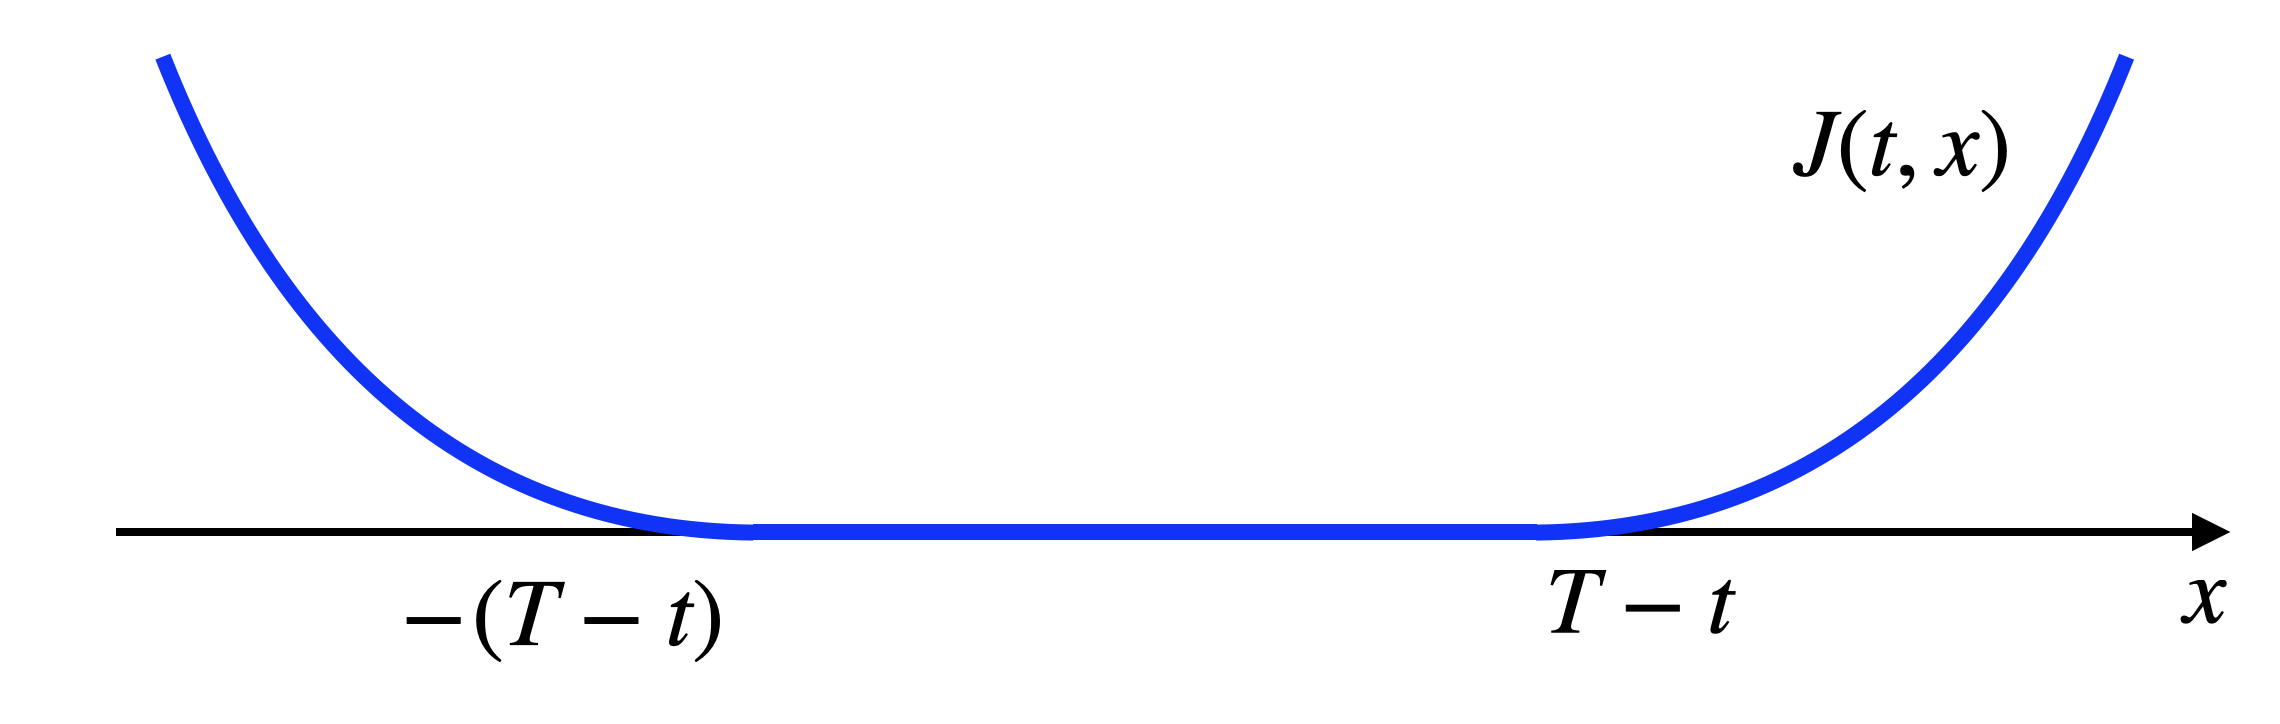
\includegraphics[width=0.6\linewidth]{images/scalar-system-optimal-J-x} 

}

\caption{Optimal cost-to-go as a function of state.}\label{fig:scalar-system-optimal-J-x}
\end{figure}

\textbf{PDE}. Substituting \eqref{eq:scalar-system-partial-J-partial-t} and \eqref{eq:scalar-system-partial-J-partial-x} into the HJB equation \eqref{eq:hjb-eqution-formal-1}, we need to verify that the followng equation holds for all \(t\) and \(x\)
\begin{equation}
0 = \min_{u \in \mathbb{U}} (1 + \text{sgn}(x) \cdot u) \max\{0, |x| - (T-t) \}.
\label{eq:scalar-system-hjb}
\end{equation}
This is easy to verify as \(u = - \text{sgn}(x)\) attains the minimum and sets the right-hand side equal to zero for any \((t,x)\).

However, we can observe that the optimal controller need not be unique. For example, when \(|x| \leq T-t\), we have
\[
\max\{0, |x| - (T-t) \} = 0,
\]
and any \(u \in \mathbb{U}\) would attain the minimum in \eqref{eq:scalar-system-hjb} and hence be optimal.
\end{example}

For simple systems, the HJB equation can be solved numerically.

\begin{example}[Numerical HJB Solution of A Scalar System]
\protect\hypertarget{exm:solve-scalar-system-numerically}{}\label{exm:solve-scalar-system-numerically}Consider a scalar linear system
\[
\dot{x} = x + u,
\]
and the optimal control problem with quadratic costs and \(T=0.5\)
\[
\min_{u(t),t\in[0,T]} x(T)^T P x(T) + \int_{t=0}^T (x^T Q x + u^T R u ) dt
\]
with \(P=Q=R=1\). Solve the HJB equation on a mesh \(x \in [-8,8]\), we obtain the optimal cost-to-go in Fig. \ref{fig:scalar-system-numerical-V}.

\begin{figure}

{\centering 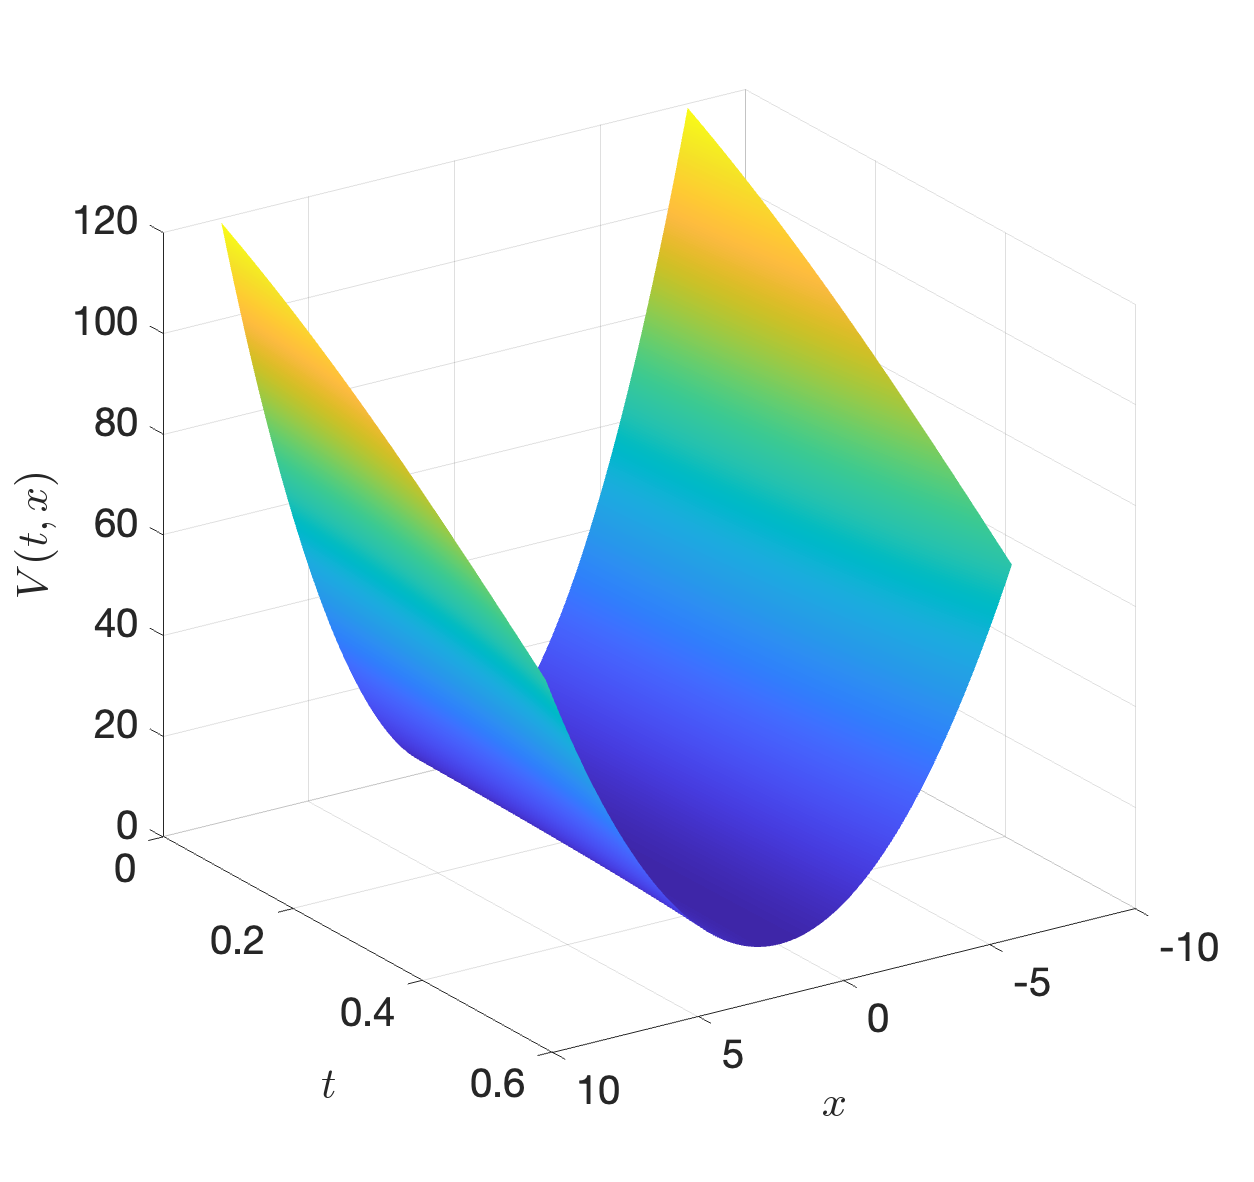
\includegraphics[width=0.6\linewidth]{images/finite_HJB_numerical_solution} 

}

\caption{Numerical solution of the HJB equation.}\label{fig:scalar-system-numerical-V}
\end{figure}

You can find code for this problem \href{https://github.com/ComputationalRobotics/OptimalControlEstimation-Examples/blob/main/finite_HJ.m}{here}.
\end{example}

\hypertarget{linear-quadratic-regulator}{%
\section{Linear Quadratic Regulator}\label{linear-quadratic-regulator}}

Let us apply the HJB sufficiency Theorem \ref{thm:hjbsufficient} to the continuous-time linear quadratic regulator (LQR).

Consider the linear system
\[
\dot{x}(t) = A x(t) + B u(t),
\]
with \(x \in \mathbb{R}^n\), \(u \in \mathbb{R}^m\), and the optimal control problem
\[
\min_{u(t),t\in [0,T]} x(T)^T P x(T) + \int_{t=0}^T (x(t)^T Q x(t) + u(t)^T R u(t)) dt 
\]
where \(P,Q\succeq 0\) and \(R \succ 0\).

According to Theorem \ref{thm:hjbsufficient}, the HJB equation for this problem is
\begin{equation}
\begin{split}
0 = \min_{u \in \mathbb{R}^m } \left[ x^T Q x + u^T R u + \nabla_t V(t,x) + \nabla_x V(t,x)^T f(x,u) \right], \quad \forall t,x, \\
V(T,x) = x^T P x, \quad \forall x.
\end{split}
\label{eq:hjb-finite-horizon-lqr}
\end{equation}

Let us guess a solution of the following form,
\[
V(t,x) = x^T S(t) x, \quad S(t) \in \mathbb{S}^n,
\]
where \(\mathbb{S}^n\) is the set of \(n \times n\) symmetric matrices.

The second equation in the HJB \eqref{eq:hjb-finite-horizon-lqr} implies
\begin{equation}
S(T) = P.
\label{eq:finite-horizon-lqr-optimal-value-terminal}
\end{equation}
The first equation in the HJB \eqref{eq:hjb-finite-horizon-lqr} requires
\begin{equation}
0 = \min_{u \in \mathbb{R}^m} \left[ x^T Q x + u^T R u + x^T \dot{S}(t) x + 2x^T S(t) (A x + Bu)  \right].
\label{eq:hjb-finite-horizon-lqr-simplify}
\end{equation}
The objective function to be minimized in \eqref{eq:hjb-finite-horizon-lqr-simplify} is a convex quadratic function of \(u\), hence the optimal solution satisfies
\[
2 R u^\star + 2B^T S(t) x = 0,
\]
solving which yields
\begin{equation}
u^\star = - R^{-1} B^T S(t) x.
\label{eq:finite-horizon-lqr-optimal-u}
\end{equation}
Now plugging the solution \eqref{eq:finite-horizon-lqr-optimal-u} back into \eqref{eq:hjb-finite-horizon-lqr-simplify}, we obtain
\[
0 = x^T \left[ \dot{S}(t) + S(t) A + A^T S(t) - S(t)B R^{-1} B^T S(t) + Q \right] x, \quad \forall (t,x),
\]
which implies that \(\dot{S}(t)\) must satisfy
\begin{equation}
\dot{S}(t) = - S(t) A - A^T S(t) + S(t) B R^{-1} B^T S(t) - Q.
\label{eq:finite-horizon-lqr-optimal-value}
\end{equation}
This is known as the \emph{continuous-time differential Riccati equation}, with the terminal condition given in \eqref{eq:finite-horizon-lqr-optimal-value-terminal}. You should compare \eqref{eq:finite-horizon-lqr-optimal-value} with its discrete-time counterpart \eqref{eq:finite-discrete-lqr-riccati} and observable their similarities.

\hypertarget{lqr-trajectory-tracking-1}{%
\subsection{LQR Trajectory Tracking}\label{lqr-trajectory-tracking-1}}

So far we have been talking about LQR in the context of regulating the system to a desired equilibrium point (usually the origin), you can in fact also use LQR for tracking a reference trajectory.

Consider again the linear system
\[
\dot{x}(t) = A x (t) + B u(t), \quad x \in \mathbb{R}^n, u \in \mathbb{R}^m.
\]
Given a reference state-control trajectory \((x_r(t),u_r(t))_{t \in [0,T]}\), we consider the following optimal control problem to track the reference trajectory
\[
\min_{u(t),t \in [0,T]} \Vert x(T) - x_r(T) \Vert_P^2 + \int_{t=0}^T \left( \Vert x(t) - x_r(t) \Vert_Q^2 + \Vert u(t) - u_r(t) \Vert_R^2  \right) dt
\]
where \(\Vert v \Vert_A^2 := v^T A v\), \(P,Q\succeq 0\) and \(R \succ 0\).

Let us guess a solution to the HJB of the following form
\[
V(t,x) = x^T S_{xx}(t) x + 2 x^T s_x(t) + s_0(t) = \begin{bmatrix} x \\ 1 \end{bmatrix}^T \underbrace{\begin{bmatrix} S_{xx}(t) & s_x(t) \\ s_x^T(t) & s_0(t) \end{bmatrix}}_{=: S(t)} \begin{bmatrix} x \\ 1 \end{bmatrix}, \quad S(t) \succ 0.
\]
Differentiating \(V(t,x)\) with respect to \(t\) and \(x\) we obtain
\begin{equation}
\begin{split}
\nabla_t V(t,x) = x^T \dot{S}_{xx}(t) x + 2 x^T \dot{s}_x(t) + \dot{s}_0(t), \\
\nabla_x V(t,x) = 2 S_{xx}(t) x + 2 s_x(t).
\end{split}
\end{equation}
Plugging the partial derivates into the HJB \eqref{eq:hjb-eqution-formal-1}, we have
\[
0 = \min_{u} \left[ \Vert x - x_r \Vert_Q^2 + \Vert u - u_r \Vert_R^2 +  \nabla_x V(t,x)^T (A x + Bu) + \nabla_t V(t,x) \right].
\]
The objective to be minimized is convex in \(u\), leading to a closed-form solution
\begin{equation}
u^{\star}(t) = u_r(t) - R^{-1}B^T \left[ S_{xx}(t)x + s_x(t) \right].
\label{eq:lqr-trajectory-tracking-solution-u}
\end{equation}
With the solution of \(u\) \eqref{eq:lqr-trajectory-tracking-solution-u} plugged back into the HJB, we can find the differential equations that \(S_{xx}(t)\), \(s_x(t)\) and \(s_0(t)\) need to satisfy
\begin{equation}
\begin{split}
-\dot{S}_{xx}(t) = Q - S_{xx}(t) B R^{-1} B^T S_{xx}(t) + S_{xx}(t)A + A^T S_{xx}(t) \\
- \dot{s}_x(t) = -Q x_r(t) + [A^T - S_{xx}(t)B R^{-1} B^T]s_x(t) + S_{xx}(t) B u_r(t) \\
- \dot{s}_0(t) = x_r(t)^T Q x_r(t) - s_x^T(t) B R^{-1} B^T s_x(t) + 2 s_x(t)^T B u_r(t),
\end{split}
\label{eq:lqr-trajectory-tracking-solution-value}
\end{equation}
with the terminal conditions
\begin{equation}
\begin{split}
S_{xx}(T) = P \\
s_x(T) = - P x_r(T) \\
s_0(T) = x_r^T(T) P x_r(T).
\end{split}
\end{equation}
Notice that the differential equation of \(S_{xx}(t)\) in \eqref{eq:lqr-trajectory-tracking-solution-value} is the same as the differential equation in \eqref{eq:finite-horizon-lqr-optimal-value}. Also notice the value of \(s_0(t)\) does not affect the optimal control \eqref{eq:lqr-trajectory-tracking-solution-u} and hence can often be ignored.

\hypertarget{lqr-trajectory-stabilization}{%
\subsection{LQR Trajectory Stabilization}\label{lqr-trajectory-stabilization}}

Recall that in Example \ref{exm:pendulum-collocation-failure}, we have seen the failure of directly applying open-loop control obtained from trajectory optimization. We then used receding horizon control to turn open-loop trajectory optimization into a close-loop controller.

Another way to stabilize the open-loop trajectory is to perform local LQR stabilization.

Given the nonlinear system
\[
\dot{x} = f(x,u),
\]
suppose we have computed a nominal state-control reference trajectory \((x_r(t),u_r(t))_{t \in [0,T]}\) (e.g., using trajectory optimization), then we can define a local coordinate system relative to the reference trajectory
\[
\bar{x}(t) = x(t) - x_r(t), \quad \bar{u}(t) = u(t) - u_r(t).
\]
The \(\bar{x}\) coordinate satisfies the following dynamics
\begin{equation}
\dot{\bar{x}} = \dot{x} - \dot{x}_r = f(x,u) - f(x_r, u_r).
\label{eq:lqr-traj-stabilization-error-dynamics}
\end{equation}
We can perform a Taylor expansion of the dynamics in \eqref{eq:lqr-traj-stabilization-error-dynamics}
\begin{equation}
\hspace{-10mm} \dot{\bar{x}} \approx f(x_r, u_r) + \frac{\partial f(x_r,u_r)}{\partial x} (x - x_r) + \frac{\partial f(x_r,u_r)}{\partial u} (u - u_r) - f(x_r, u_r) = A(t) \bar{x} + B(t) \bar{u},
\label{eq:lqr-traj-stabilization-error-dynamics-linear}
\end{equation}
where
\[
A(t) = \frac{\partial f(x_r(t),u_r(t))}{\partial x}, \quad B(t) = \frac{\partial f(x_r(t),u_r(t))}{\partial u},
\]
are time-varying linear matrices.

We then formulate the LQR problem for the approximate linear time-varying system \eqref{eq:lqr-traj-stabilization-error-dynamics-linear}
\begin{equation}
\min_{\bar{u}(t), t \in [0,T]} \bar{x}(T)^T P \bar{x}(T) + \int_{t=0}^T \left( \bar{x}(t)^T Q \bar{x}(t) + \bar{u}(t)^T R \bar{u}(t)  \right) dt
\label{eq:lqr-traj-stabilization-ocp}
\end{equation}
with \(P \succeq 0, Q \succeq 0, R \succ 0\). The solution to \eqref{eq:lqr-traj-stabilization-ocp}, according to \eqref{eq:finite-horizon-lqr-optimal-u} is
\[
\bar{u}(t) = - R^{-1} B^T S(t) \bar{x},
\]
which implies
\begin{equation}
u(t) = u_r(t) - R^{-1} B^T S(t) (x(t) - x_r(t))
\label{eq:lqr-traj-stabilization-ocp-solution-u-abs}
\end{equation}
in the original coordinates. Note that the controller in \eqref{eq:lqr-traj-stabilization-ocp-solution-u-abs} is a feedback controller that ``finetunes'' the open-loop control.

\hypertarget{the-pontryagin-minimum-principle}{%
\section{The Pontryagin Minimum Principle}\label{the-pontryagin-minimum-principle}}

The HJB equation in Theorem \ref{thm:hjbsufficient} provides a \emph{sufficient} condition for the optimal cost-to-go. However, since the HJB equation is a sufficient condition, there do exist cases where the optimal cost-to-go does not satisfy the HJB equation but is still optimal (e.g., when the optimal cost-to-go is not continuously differentiable).

We now introduce a \emph{necessary} condition that any optimal control trajectory and state trajectory must satisfy. This condition is the celebrated Pontryagin minimum principle.

A rigorous derivation of the Pontryagin minimum principle can be mathematically involving and is beyond the scope of this lecture notes (see Section 7.3.2 in \citep{bertsekas12book-dpocI} for a more rigorous treatment). In the following, we provide an informal derivation of the Pontryagin minimum principle.

Recall the HJB equation in Theorem \ref{thm:hjbsufficient} states that, if a control trajectory \(u^\star(t)\) and the associated state trajectory \(x^\star(t)\) is optimal, then for all \(t \in [0,T]\), the following condition must hold
\begin{equation}
u^\star(t) = \arg\min_{u \in \mathbb{U}} \left[ g(x^\star(t),u) + \nabla_x J(t,x^\star(t))^T f(x^\star(t),u)  \right] 
\label{eq:pmp-intro-from-hjb}.
\end{equation}
The above equation says, in order to compute the optimal control, we do not need to know the value of \(\nabla_x J\) at \emph{all} possible values of \(x\) and \(t\) (which is what the HJB equation tries to do), and we only need to know the value of \(\nabla_x J\) along the \emph{optimal} trajectory, i.e., to know only \(\nabla_x J(t,x^\star(t))\).

The Pontryagin minimum principle builds upon this key observation, and it points out that \(\nabla_x J(t,x^\star(t))\) (but not \(\nabla_x J(t,x)\) for any \(x\)) satisfies a certain differential equation called the \emph{adjoint equation}.

We now provide an informal derivation of the adjoint equation that is based on differentiating the HJB equation. Towards this goal, we first present the following lemma which is itself quite useful.

\begin{lemma}[Differentiating Functions Involving Minimization]
\protect\hypertarget{lem:gradientofminimumfunctions}{}\label{lem:gradientofminimumfunctions}Let \(F(t,x,u)\) be a continuously differentiable function of \(t \in \mathbb{R}\), \(x \in \mathbb{R}^n\), \(u \in \mathbb{R}^m\), and let \(\mathbb{U}\) be a convex subset of \(\mathbb{R}^m\). Suppose \(\mu^\star(t,x)\) is a continuously differentiable function such that
\[
\mu^\star(t,x) = \arg\min_{u \in \mathbb{U}} F(t,x,u), \quad \forall t,x.
\]
Then
\begin{align}
\nabla_t \left\{ \min_{u \in \mathbb{U}} F(t,x,u) \right\} = \nabla_t F(t,x,\mu^\star(t,x)), \quad \forall t,x, \\
\nabla_x \left\{ \min_{u \in \mathbb{U}} F(t,x,u) \right\} = \nabla_x F(t,x,\mu^\star(t,x)), \quad \forall t,x.
\end{align}
In words, the partial derivates (with respect to \(t\) and \(x\)) of ``the minimum of \(F(t,x,u)\) over \(u\)'' (commonly known in optimization as the value function \(\psi(t,x)\) of \(F(t,x,u)\)) are equal to the partial derivates of \(F(t,x,u)\) (with respect to \(t\) and \(x\)) after plugging in the optimizer \(\mu^\star(t,x)\).
\end{lemma}

We now start with the HJB equation in \eqref{eq:hjb-eqution-formal-1}, restated below with \(V(t,x)\) replaced by the optimal \(J(t,x)\) for the reader's convenience
\begin{equation}
0 = \min_{u \in \mathbb{U}} \left[ g(x,u) + \nabla_t J(t,x) + \nabla_x J(t,x)^Tf(x,u)  \right].
\label{eq:hjb-equation-restate-for-pmp}
\end{equation}
Assume that \(\mu^\star(t,x)\) attains the minimum in the equation above and it is also continuously differentiable. Note that we have made the restrictive assumption that \(\mathbb{U}\) is convex and \(\mu^\star(t,x)\) is continuously differentiable, which are not necessary in a more rigorous derivation of Pontryagin's principle (cf.~Section 7.3.2 in \citep{bertsekas12book-dpocI}).

We differentiate both sides of \eqref{eq:hjb-equation-restate-for-pmp} with respect to \(t\) and \(x\). In particular, let
\[
F(t,x,u) = g(x,u) + \nabla_t J(t,x) + \nabla_x J(t,x)^T f(x,u)
\]
and invoke Lemma \ref{lem:gradientofminimumfunctions}, we can write
\begin{align}
\label{eq:hjb-equation-differentiation-x}
\hspace{-12mm}
0 = \nabla_x g(x, \mu^\star(t,x)) + \nabla^2_{xt} J(t,x) + \nabla^2_{xx} J(t,x)f(x,\mu^\star(t,x)) + \nabla_x f(x,\mu^\star(t,x)) \nabla_x J(t,x).\\
\hspace{-12mm} 0 = \nabla^2_{tt}J(t,x) + \nabla_{xt}^2 J(t,x)^T f(x,\mu^\star(t,x)) 
\label{eq:hjb-equation-differentiation-t}
\end{align}
where the first equation results from differentiation of \eqref{eq:hjb-equation-restate-for-pmp} with respect to \(x\), and the second equation results from differentiation of \eqref{eq:hjb-equation-restate-for-pmp} with respect to \(t\). In \eqref{eq:hjb-equation-differentiation-x}, \(\nabla_x f(x,\mu^\star(t,x))\) is
\[
\nabla_f = \begin{bmatrix}
\frac{\partial f_1}{\partial x_1} & \cdots & \frac{\partial f_n}{x_1} \\
\vdots & \ddots & \vdots \\
\frac{\partial f_1}{\partial x_n} & \cdots & \frac{\partial f_n}{\partial x_n}
\end{bmatrix}
\]
evaluated at \((x,\mu^\star(t,x))\).
Equations \eqref{eq:hjb-equation-differentiation-x} and \eqref{eq:hjb-equation-differentiation-t} hold for any \((t,x)\) (under the restrictive assumptions we have made).

We then evaluate the equations \eqref{eq:hjb-equation-differentiation-x} and \eqref{eq:hjb-equation-differentiation-t} only along the optimal control and state trajectory \((u^\star(t),x^\star(t))\) that satisfies
\begin{equation}
\dot{x}^\star(t) = f(x^\star(t),u^\star(t)), \quad u^\star(t) = \mu^\star(t,x^\star(t)), \quad t \in [0,T].
\label{eq:pmp-optimal-system-dynamics}
\end{equation}
Specifically, along the optimal trajectory, we have
\[
\frac{d}{dt} \left( \nabla_x J(t,x^\star(t)) \right) = \nabla^2_{xt} J(t,x^\star(t)) + \nabla^2_{xx} J(t,x^\star(t))f(x^\star(t),u^\star(t)),
\]
where the right-hand side contains terms in the right-hand side of \eqref{eq:hjb-equation-differentiation-x} (when evaluted along the optimal trajectory). Similarly,
\[
\frac{d}{dt} \left( \nabla_t J(t,x^\star(t)) \right) = \nabla^2_{tt} J(t,x^\star(t)) + \nabla^2_{xt} J(t,x^\star(t))^T f(x^\star(t),u^\star(t)),
\]
where the right-hand side is exactly the right-hand side of \eqref{eq:hjb-equation-differentiation-t} (when evaluted along the optimal trajectory). As a result, equations \eqref{eq:hjb-equation-differentiation-x} and \eqref{eq:hjb-equation-differentiation-t}, when evaluated along the optimal trajectory, are equivalent to
\begin{align}
\label{eq:hjb-equation-differentiation-along-optimal-x}
0 = \nabla_x g(x^\star(t), u^\star(t)) + \frac{d}{dt}\left( \nabla_x J(t,x^\star(t)) \right) + \nabla_x f(x^\star(t),u^\star(t)) \nabla_x J(t,x^\star(t)).\\
0 = \frac{d}{dt}\left( \nabla_t J(t,x^\star(t)) \right).
\label{eq:hjb-equation-differentiation-along-optimal-t}
\end{align}
Therefore, if we denote
\[
p(t) = \nabla_x J(t,x^\star(t)), \quad p_0(t) = \nabla_t J(t,x^\star(t)),
\]
then equations \eqref{eq:hjb-equation-differentiation-along-optimal-x} and \eqref{eq:hjb-equation-differentiation-along-optimal-t} become
\begin{align}
\label{eq:adjoint-equation-p}
\dot{p}(t) = - \nabla_x f(x^\star(t),u^\star(t)) p(t) - \nabla_x g(x^\star(t),u^\star(t)), \\
\dot{p}_0(t) = 0.
\label{eq:adjoint-equation-p0}
\end{align}
Equation \eqref{eq:adjoint-equation-p}, which is a system of \(n\) first-order differential equations, is known as the adjoint equation and it describes the evolution of \(p(t)\), known as the \emph{costate}, along the optimal trajectory. To obtain a boundary condition for the adjoint equation \eqref{eq:adjoint-equation-p}, we note that the boundary condition of the HJB equation
\[
J(T,x) = h(x),\quad \forall x
\]
implies
\[
p(T) = \nabla h(x^\star(T)).
\]

This is basically the Pontryagin Minimum Principle.

\textbf{The Hamiltonian formulation}. It is usually more convenient to state the Pontryagin Principle using the concept of a \emph{Hamiltonian}. Formally, we define the Hamiltonian function that maps the triplet \((x,u,p) \in \mathbb{R}^n \times \mathbb{R}^m \times \mathbb{R}^n\) to real numbers given by
\[
H(x,u,p) = g(x,u) + p^T f(x,u).
\]
Note that the dynamics along the optimal trajectory \eqref{eq:pmp-optimal-system-dynamics} can be conveniently written as
\[
\dot{x}^\star(t) = \nabla_p H(x^\star(t),u^\star(t),p(t)),
\]
and the adjoint equation \eqref{eq:adjoint-equation-p} can be written as
\[
\dot{p}(t) = - \nabla_x H(x^\star(t), u^\star(t), p(t)).
\]
We are now ready to state the Pontryagin Minimum Principle.

\begin{theorem}[Pontryagin Minimum Principle as A Necessary Condition for Optimality]
\protect\hypertarget{thm:pontryaginminimum}{}\label{thm:pontryaginminimum}Let \((u^\star(t), x^\star(t)), t \in [0,T]\) be a pair of optimal control and state trajectories satisfying
\[
\dot{x}^\star(t) = f(x^\star(t),u^\star(t)), \quad x^\star(0) = x_0 \text{ given}.
\]
Let \(p(t)\) be the solution of the adjoint equation
\[
\dot{p}(t) = - \nabla_x H(x^\star(t),u^\star(t),p(t)),
\]
with the boundary condition
\[
p(T) = \nabla h(x^\star(T)),
\]
where \(h\) is the terminal cost function. Then, for all \(t \in [0,T]\), we have
\[
u^\star(t) = \arg\min_{u \in \mathbb{U}} H(x^\star(t),u,p(t)).
\]
Moreover, there is a constant \(C\) such that
\[
H(x^\star(t),u^\star(t),p(t)) = C, \quad \forall t \in [0,T].
\]
\end{theorem}

To see why \(H(x^\star(t),u^\star(t),p(t))\) is a constant along the optimal trajectory, we observe that from the HJB equation \eqref{eq:hjb-equation-restate-for-pmp}, we obtain
\begin{align}
g(x^\star,u^\star) + \nabla_t J(t,x^\star) + \nabla_x J(t,x^\star)^T f(x^\star, u^\star) = 0 \\
\Longrightarrow \underbrace{g(x^\star,u^\star) + \nabla_x J(t,x^\star)^T f(x^\star, u^\star)}_{H(x^\star(t),u^\star(t),p(t))} = - \underbrace{\nabla_t J(t,x^\star)}_{p_0(t)}.
\end{align}
From \eqref{eq:adjoint-equation-p0}, we know \(p_0(t)\) is a constant.

\textbf{A necessary condition}. It is important to recognize that the Pontryagin Minimum Principle in Theorem \ref{thm:pontryaginminimum} is a necessary condition for optimality, i.e., all optimal control and state trajectories must satisfy this condition, but \emph{not all} trajectories satisfying the condition are optimal. Extra arguments are needed to guarantee optimality. One common strategy is to show that an optimal control trajectory exists, and then verify that there is only one control trajectory satisfying the conditions of the Minimum Principle (or that all trajectories verifying the Minimum Principle have equal costs). A setup where the Minimum Principle is both necessary is sufficient is when \(f(x,u)\) is linear in \((x,u)\), the the constraint set \(U\) is convex, and the cost functions \(h\) and \(g\) are convex.

\textbf{Two-point boundary value problem} (TPBVP). The Pontryagin Minimum Principle is particularly useful when
\begin{equation}
u^\star = \arg\min_{u \in \mathbb{U}} H(x^\star,u,p) = \arg\min_{u \in \mathbb{U}} g(x^\star,u) + p^T f(x^\star,u)
\label{eq:pmp-solve-u-from-H}
\end{equation}
can be solved analytically so that \(u^\star\) becomes a function of \(x^\star\) and \(p\). For example, this is possible when problem \eqref{eq:pmp-solve-u-from-H} is a convex problem, for which one can invoke the KKT optimality conditions (cf.~Appendix \ref{appconvex-theory-kkt}). Once \(u^\star(t)\) is expressed as a function of \(x^\star(t)\) and \(p(t)\), we can merge the system equation \eqref{eq:pmp-optimal-system-dynamics} and the adjoint equation \eqref{eq:adjoint-equation-p} together and arrive at
\begin{equation}
\begin{cases}
\dot{x}^\star(t) = f(x^\star(t), u^\star(t)) \\
\dot{p}(t) = - \nabla_x f(x^\star(t),u^\star(t)) p(t) - \nabla_x g(x^\star(t),u^\star(t))
\end{cases},
\label{eq:two-point-boundary-problem}
\end{equation}
which is a set of \(2n\) first-order differential equations in \(x^\star(t)\) and \(p(t)\). The boundary conditions are
\begin{equation}
x^\star(0) = x_0, \quad p(T) = \nabla h(x^\star(T)).
\label{eq:two-point-boundary-problem-boundary}
\end{equation}
The number of boundary conditions is also \(2n\), so generally we expect to be able to solve these differential equations numerically.

\begin{example}[Shortest Curve]
\protect\hypertarget{exm:shortest-line}{}\label{exm:shortest-line}In Fig. \ref{fig:shortest-curve}, consider any curve that starts at the point \((0,\alpha)\) and lands on the vertical line that passes through \((T,0)\). What is the curve with minimum length?

We all know the answer is a straight line.

\begin{figure}

{\centering 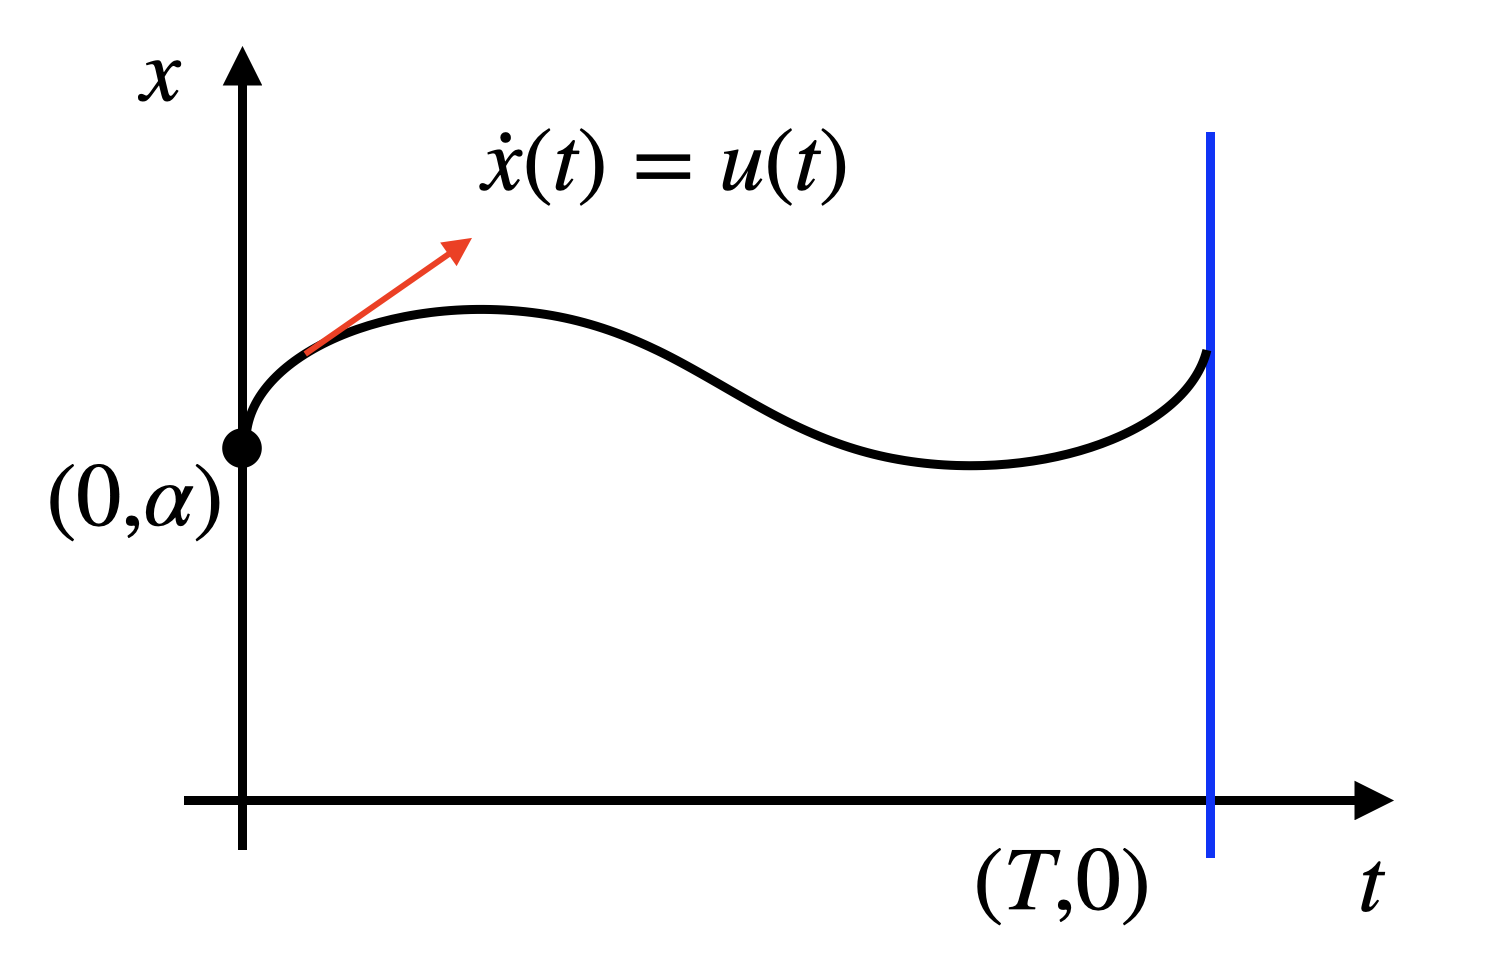
\includegraphics[width=0.6\linewidth]{images/shortest_path} 

}

\caption{Shortest curve between a point and a line.}\label{fig:shortest-curve}
\end{figure}

Let us use Pontryagin's minimum principle to prove this. The length of any curve satisfying our condition is
\[
\int_{0}^{T} \sqrt{1 + (\dot{x}(t))^2} dt, \quad x(0) = \alpha.
\]
To find the curve with minimum length, we can formulate an optimal control problem
\[
\min_{u(t)} \int_{t=0}^T \sqrt{ 1 + u^2(t)} dt, \quad \text{subject to} \quad \dot{x}(t) = u(t), x(0) = \alpha.
\]

To apply Pontryagin's minimum principle, we first formulate the Hamiltonian
\[
H(x,u,p) = g(x,u) + p^T f(x,u) = \sqrt{1 + u^2} + pu.
\]
The adjoint equation says
\[
\dot{p}(t) = - \nabla_x H(x^\star(t),u^\star(t),p),
\]
which simplifies, for our problem, to
\[
\dot{p}(t) = 0.
\]
The boundary condition of the adjoint equation is
\[
p(T) = \nabla h(x^\star(T)) = 0.
\]
We conclude that
\[
p(t) = 0, \forall t \in [0,T].
\]
The optimal controller thus becomes
\[
u^\star(t) = \arg\min_u H(x^\star(t),u,p(t)) = \arg\min_u \sqrt{1 + u^2} = 0, \quad \forall t \in [0,T].
\]
Therefore, we have \(\dot{x}^\star(t) = u^\star(t) = 0\) for all \(t \in [0,T]\), and \(x^\star(t) = \alpha\) for all time, which is a straight line.
\end{example}

\hypertarget{numerical-solution-of-the-tpbvp}{%
\subsection{Numerical Solution of the TPBVP}\label{numerical-solution-of-the-tpbvp}}

When the optimal control can be solved analytically, we obtain the two-point boundary value problem (TPBVP)
\begin{equation}
\begin{cases}
x^\star(0) = x_0 \\
p(T) = \nabla h(x^\star(T)) \\
\dot{x}^\star(t) = f(x^\star(t), u^\star(t)) \\
\dot{p}(t) = - \nabla_x f(x^\star(t),u^\star(t))p(t) - \nabla_x g(x^\star(t),u^\star(t))
\end{cases},
\label{eq:two-point-boundary-value-problem}
\end{equation}
where \(u^\star(t)\) is a function of \(x^\star(t)\) and \(p(t)\). Calling
\[
z(t) = \begin{bmatrix} x^\star(t) \\ p(t) \end{bmatrix},
\]
we can compactly write \eqref{eq:two-point-boundary-value-problem} as
\begin{equation}
\begin{cases}
b(z(0),z(T),x_0) = 0 \\
\dot{z}(t) - \phi(z(t)) = 0
\end{cases},
\label{eq:two-point-boundary-value-problem-simple}
\end{equation}
which has \(2n\) differential equations and \(2n\) boundary conditions and usually well defined.

\hypertarget{single-shooting}{%
\subsubsection{Single Shooting}\label{single-shooting}}

The idea of single shooting is straightforward: if \(p(0)\) is known in \eqref{eq:two-point-boundary-value-problem}, then (i) the entire trajectory of \(z\) can be simulated forward in time, and (ii) we only need to enforce the terminal constraint of \(p(T) = \nabla h(x^\star(T))\).

Therefore, in single shooting, we denote the terminal residual
\[
r_T = p(T) - \nabla h(x^\star(T)) = r_T(p_0),
\]
as a function of \(p(0) = p_0\) (note that evaluating this function requires simulating \(\dot{z}(t) = \phi(z(t))\)). Then we use \href{https://en.wikipedia.org/wiki/Newton\%27s_method}{Newton's method} to iteratively update \(p_0\) via
\[
p_0^{(k+1)} = p_0^{(k)} - \eta_k \left( \frac{\partial r_T}{\partial p_0}(p_0^{(k)}) \right)^{-1} r_T(p_0^{(k)}),
\]
where \(\eta_k\) is a chosen step size.

In some cases, the forward simulation of the combined ODE might be an ill-conditioned problem so that single shooting cannot be employed. Even if the forward simulation problem is well-defined, the region of attraction of the Newton iteration can be very small, such that a good guess for \(p_0\) is often required.

\hypertarget{multiple-shooting}{%
\subsubsection{Multiple Shooting}\label{multiple-shooting}}

The single shooting method also suffers from the nonlinearity and inaccuracy brought by simulating the ODE for a long time duration \(T\).

In multiple shooting, we break the time windown \([0,T]\) into \(N\) pieces such that
\[
0 = t_0 \leq \dots \leq t_k \leq t_{k+1} \leq \dots \leq t_N = T.
\]
We then assign values
\[
z_k = z(t_k), k = 0,\dots,N,
\]
as the values of \(z(t)\) at those breakpoints. The values \(z_k\) should satisfy the ODE
\[
z_{k+1} = \Phi(z_k),
\]
where \(\Phi(\cdot)\) integrates the ODE from time \(t_k\) to \(t_{k+1}\) with initial condition \(z_k\).

We can then form a system of equations on \(z=(z_0,\dots,z_N)\) as
\begin{equation}
\begin{cases}
b(z_0,z_N,x_0) = 0 \\
z_{k+1} - \Phi(s_k) = 0 
\end{cases}.
\end{equation}
Denoting the vector of residuals as
\[
R(z,x_0) = \begin{bmatrix} b(z_0,z_N,x_0) \\ z_{k+1} - \Phi(s_k) \end{bmatrix},
\]
we can use Newton's method to iteratively solve \(z\):
\begin{equation}
z^{(k+1)} = z^{(k)} - \eta_k \left( \frac{\partial R}{\partial z}(z^{(k)}) \right)^{-1} R(z^{(k)}).
\end{equation}

\hypertarget{collocation}{%
\subsubsection{Collocation}\label{collocation}}

\hypertarget{infinite-horizon-problems}{%
\section{Infinite-Horizon Problems}\label{infinite-horizon-problems}}

\hypertarget{continuous-time-infinite-horizon-lqr}{%
\subsection{Infinite-Horizon LQR}\label{continuous-time-infinite-horizon-lqr}}

Consider a linear time-invariant system
\[
\dot{x} = Ax + Bu,
\]
and the infinite-horizon optimal control problem
\[
\min \int_{t=0}^{\infty} (x(t)^T Q x(t) + u(t)^T R u(t)) dt, \quad x(0) = x_0.
\]
with \(Q \succeq 0, R \succ 0\).
The optimal controller takes the following linear feedback form
\[
u = - R^{-1}B^T S x,
\]
with \(S\) the solution to the continuous-time algebraic Riccati equation
\[
0 = SA + A^T S - SBR^{-1} B^T S + Q.
\]
In Matlab, given \(A,B,Q,R\), you can use \href{https://www.mathworks.com/help/control/ref/lti.lqr.html}{\texttt{lqr}} to compute \(K\) and \(S\).

\hypertarget{viscosity-solution}{%
\section{Viscosity Solution}\label{viscosity-solution}}

\hypertarget{stability}{%
\chapter{Stability Analysis}\label{stability}}

Optimal control formulates a control problem via the language of mathematical optimization. However, there are control problems, and sometimes even the very basic control problems, that cannot be easily stated in the optimal control formulation.

For example, suppose our goal is to \emph{swing up a pendulum to the upright position and stabilize it there}. You may want to formalize the problem as
\begin{equation}
\min_{u(t) \in \mathbb{U}} \int_{0}^{\infty} \Vert x(t) - x_d \Vert^2 dt, \quad \text{subject to} \quad \dot{x} = f(x,u), x(0) = x_0,
\label{eq:pendulum-swingup-stability-test-1}
\end{equation}
where \(x_d\) is the desired upright position for the pendulum. However, does the solution of problem \eqref{eq:pendulum-swingup-stability-test-1}, if exists, guarantee the stabilization of the pendulum at the upright position? The answer is unclear without a rigorous proof.

However, after a slight change of perspective, the optimal control problem may be formulated to better match the goal. Suppose there exists a region, \(\Omega\), in the state space such that as long as the pendulum enters \(\Omega\), there always exists a sequence of control to bring the pendulum to the goal state \(x_d\), then we can simply formulate a different optimal control problem
\begin{equation}
\min_{u(t) \in \mathbb{U}} \int_{0}^{T} \Vert u(t) \Vert^2 dt, \quad \text{subject to} \quad x(0)=x_0, x(T) \in \Omega, \dot{x} = f(x,u),
\label{eq:pendulum-swingup-stability-test}
\end{equation}
where now it is very clear, if a solution exists to problem \eqref{eq:pendulum-swingup-stability-test}, then we will definitely achieve our goal. This is because the constraint \(x(T) \in \Omega\) guarantees that we will be able to stabilize the pendulum, and the cost function of \eqref{eq:pendulum-swingup-stability-test} simply encourages minimum control effort along the way.

This highlights that, sometimes the formulation of a problem may deserve more thoughts than the actual solution. Of course the formulation \eqref{eq:pendulum-swingup-stability-test} may be much more difficult to solve. In fact, does the set \(\Omega\) exist, and if so, how to describe it?

This is the main focus of this chapter: to introduce tools that can help us analyze the \emph{stability} of uncontrolled and controlled nonlinear systems. Specifically, we will introduce the notion of \emph{stability certificates}, which are conditions that, if hold, certify the stability of the system (e.g., in the set \(\Omega\)). Interestingly, you will see that the notion of stability certificates is intuitive and easy, but what is really challenging is to \emph{find} and \emph{compute} the stability certificates. We will highlight the power and also limitation of computational tools, especially those that are based on convex optimization (see Appendix \ref{appconvex} for a review of convex optimization).

\hypertarget{autonomous-systems}{%
\section{Autonomous Systems}\label{autonomous-systems}}

Let us first focus on autonomous systems, i.e., systems whose dynamics do not depent on time (and control). We introduce different concepts of stability and ways to certify them.

\hypertarget{concepts-of-stability}{%
\subsection{Concepts of Stability}\label{concepts-of-stability}}

Consider the autonomous system
\begin{equation}
\dot{x} = f(x)
\label{eq:autonomous-system}
\end{equation}
where \(x \in \mathbb{X} \subseteq \mathbb{R}^n\) is the state and \(f: \mathbb{R}^n \rightarrow \mathbb{R}^n\) is the (potentially nonlinear) dynamics.

Before talking about concepts of stability, we need to define an \emph{equilibrium point}.

\begin{definition}[Equilibrium Point]
\protect\hypertarget{def:equilibriumpoint}{}\label{def:equilibriumpoint}A state \(x^\star\) is called an equilibrium point of system \eqref{eq:autonomous-system} if \(f(x^\star) = 0\), i.e., once the system reaches \(x^\star\), it stays at \(x^\star\).
\end{definition}

For example, a linear system
\[
\dot{x} = A x
\]
has a single equilibrium point \(x^\star = 0\) when \(A\) is nonsingular, and an infinite number of equilibrium points when \(A\) is singular (those equilibrium points lie in the kernel of matrix \(A\)).

When analyzing the behavior of a dynamical system around the equilibrium point, it is often helpful to ``shift'' the dynamics equation so that \(0\) is the equilibrium point. For example, if we are interested in the behavior of system \eqref{eq:autonomous-system} near the equilibrium point \(x^\star\), we can create a new variable
\[
z = x - x^\star,
\]
so that
\begin{equation}
\dot{z} = \dot{x} = f(x) = f(z + x^\star).
\label{eq:shifted-system-by-equilibrium}
\end{equation}
Clearly, \(z^\star = 0\) is an equilibrium point for the shifted system \eqref{eq:shifted-system-by-equilibrium}.

Let us find the equilibrium points of a simple pendulum.

\begin{example}[Equilibrium Points of A Simple Pendulum]
\protect\hypertarget{exm:pendulumequilibriumpoint}{}\label{exm:pendulumequilibriumpoint}Consider the dynamics of an uncontrolled pendulum

\begin{equation}
\begin{cases}
\dot{\theta} = \dot{\theta} \\
\ddot{\theta} = - \frac{1}{ml^2} (b \dot{\theta} + mgl \sin \theta)
\end{cases}
\label{eq:pendulum-dynamics-for-equilibrium-point}
\end{equation}
where \(\theta\) is the angle between the pendulum and the vertical line, and \(x = [\theta,\dot{\theta}]^T\) is the state of the pendulum (\(m,g,l,b\) denote the mass, gravity constant, length, and damping constant, respectively).

To find the equilibrium points of the pendulum, we need the right hand sides of \eqref{eq:pendulum-dynamics-for-equilibrium-point} to be equal to zero:
\[
\dot{\theta} = 0, \quad - \frac{1}{ml^2} (b \dot{\theta} + mgl \sin \theta) = 0.
\]
The solutions are easy to find
\[
x^\star = \begin{bmatrix} 0 \\ 0 \end{bmatrix} \quad \text{or} \quad \begin{bmatrix} \pi \\ 0 \end{bmatrix},
\]
corresponding to the bottomright and upright positions of the pendulum, respectively.
\end{example}

The pendulum dynamics has two equilibrium points, but our physics intuition tells us these two equilibrium points are dramatically different. Specifically, the bottomright equilibrium \(x^\star = [0,0]^T\) is such that if you perturb the pendulum around the equilibrium, the pendulum will go back to that equilibrium; the upright equilibrium \(x^\star = [\pi,0]^T\) is such that if you perturb the pendulum (even just a little bit) around the equilibrium, it will diverge from that equilibrium.

This physical intuition is exactly what we want to formalize as the concepts of stability.

In the following, we focus on the nonlinear autonomous system \eqref{eq:autonomous-system} with \(f(0) = 0\), i.e., \(x^\star = 0\) is an equilibrium point. We now formally define the different concepts of stability.

\begin{definition}[Lyapunov Stability]
\protect\hypertarget{def:lyapunovstability}{}\label{def:lyapunovstability}The equilibrium point \(x=0\) is said to be \emph{stable in the sense of Lyapunov} if, for any \(R > 0\), there exists \(r >0\) such that if \(\Vert x(0) \Vert < r\), then \(\Vert x(t) \Vert < R\) for all \(t \geq 0\). Otherwise, the equilibrium point is unstable.
\end{definition}

For a system that is Lyapunov stable around \(x=0\), the definition says that, if we want to constrain the trajectory of the system to be within the ball \(B_R = \{ x \mid \Vert x \Vert < R \}\), then we can always find a smaller ball \(B_r = \{ x \mid \Vert x \Vert < r \}\) such that if the system starts within \(B_r\), it will remain in the larger ball \(B_R\).

On the other hand, if the system is not Lyapunov stable at \(x=0\), then there exists at least one ball \(B_R\), such that no matter how close the system's initial condition is to the origin, it will eventually exit the ball \(B_R\). The following exercise is left for you to verify the instability of the Van der Pol oscillator.

\begin{exercise}[Instability of the Van der Pol oscillator]
\protect\hypertarget{exr:instabilityvanderpol}{}\label{exr:instabilityvanderpol}Show that the Van der Pol oscillator
\[
\begin{cases}
\dot{x}_1 = x_2 \\
\dot{x}_2 = - x_1 + (1-x_1^2) x_2
\end{cases}
\]
is unstable at the equilibrium point \(x = 0\).
\end{exercise}

Lyapunov stability does not guarantee the system trajectory will actually converge to \(x =0\). Instead, asymptotic stability will ask the system trajectory to converge to \(x=0\).

\begin{definition}[Asymptotic Stability and Domain of Attraction]
\protect\hypertarget{def:asymptoticstability}{}\label{def:asymptoticstability}The equilibrium point \(x = 0\) is said to be \emph{asymptotically stable} if (i) it is Lyapunov stable, and (ii) there exists some \(r > 0\) such that \(x(0) \in B_r\) implies \(x(t) \rightarrow 0\) as \(t \rightarrow \infty\).

\emph{The} domain of attraction (for the equilibrium \(x=0\)) is the largest set of points in the state space such that trajectories initiated at those points will converge to the equilibrium point. That is,
\[
\Omega(x^\star) = \{ x \in \mathbb{X} \mid x(0) = x \Longrightarrow \lim_{t \rightarrow \infty} x(t) = x^\star \}.
\]
The ball \(B_r\) is \emph{a} domain of attraction for the equilibrium point \(x=0\), but not necessarily the largest domain of attraction.
\end{definition}

You may immediately realize that in the definition of asymptotic stability, we require Lyapunov stability to hold first. Is this necessary? i.e., does there exist a system where trajectories eventually converge to zero, but is not stable in the sense of Lyapunov? You should work out the following exercise.

\begin{exercise}[Vinograd System]
\protect\hypertarget{exr:vinogradequation}{}\label{exr:vinogradequation}

Show that for the Vinograd dynamical system \citep{vinograd57-inapplicability}
\[
\begin{cases}
\dot{x} = \frac{x^2(y-x) + y^5}{(x^2+y^2)(1 + (x^2+y^2)^2)} \\
\dot{y} = \frac{y^2 (y - 2x)}{(x^2+y^2)(1 + (x^2+y^2)^2)}
\end{cases},
\]
all system trajectories converge to the equilibrium point \((x,y) = 0\), but the equilibrium point is not stable in the sense of Lyapunov.

(Hint: the system trajectories will behave like the following plot.)

\begin{figure}

{\centering 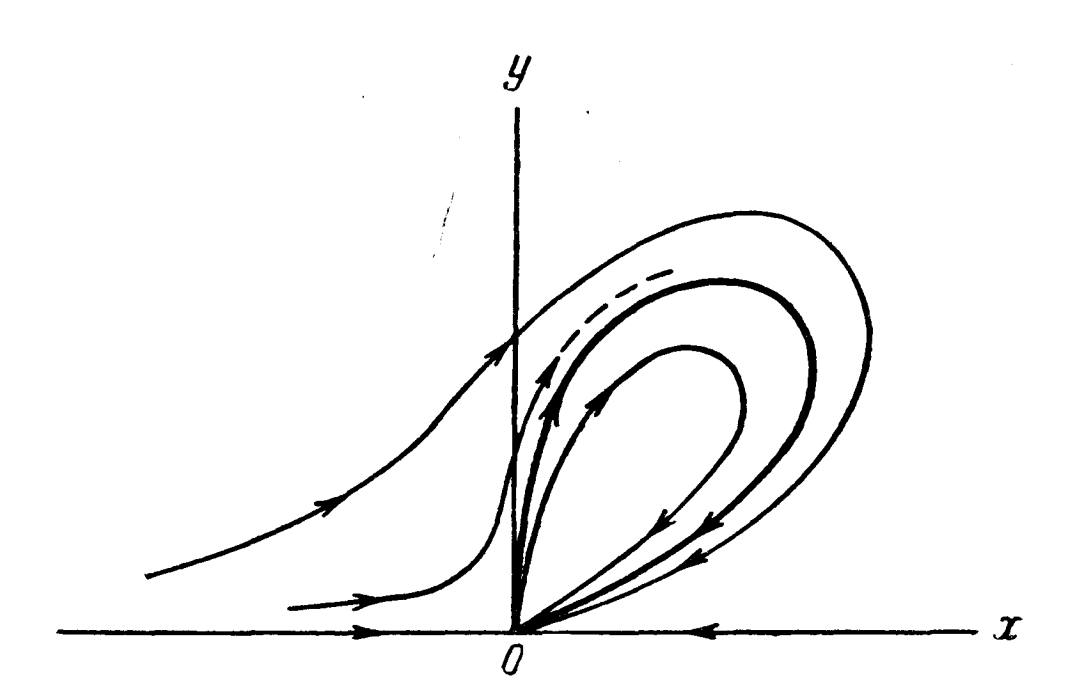
\includegraphics[width=0.6\linewidth]{images/vinograd} 

}

\caption{Trajectories of the Vinograd system. Copied from the original article of Vinograd.}\label{fig:vinograd-system}
\end{figure}

\end{exercise}

In many cases, we want the convergence of the system trajectory towards \(x=0\) to be fast, thus bringing in the notion of exponential stability.

\begin{definition}[Exponential Stability]
\protect\hypertarget{def:exponentialstability}{}\label{def:exponentialstability}An equilibrium point \(x=0\) is said to be exponentially stable, if there exists a ball \(B_r\) such that as long as as \(x(0) \in B_r\), then
\[
\Vert x(t) \Vert \leq \alpha \Vert x(0) \Vert e^{-\lambda t}, \quad \forall t,
\]
for some \(\alpha > 0\) and \(\lambda > 0\) (\(\lambda\) is called the rate of exponential convergence).
\end{definition}

Exponential stability implies asymptotic stability (and certainly also Lyapunov stability). What is nice about exponential stability is that we can quantify the distance of the system trajectory to the equilibrium point as a function of time (as long as we know the constants \(\alpha, \Vert x(0) \Vert, \lambda\)). In many safety-critical applications, we need such performance guarantees. For example, in Chapter \ref{state-observer}, we will see the application of exponential stability in observer-feedback control.

All the concepts of stability we have mentioned so far only talk about the stability of the system \emph{locally} around the equilibrium point \(x=0\) (via arguments like \(B_r\) and \(B_R\)). It would be much nicer if we can guarantee stability of the system \emph{globally}, i.e., no matter where the system starts in the state space \(\mathbb{X}\), its trajectoy will converge to \(x=0\).

\begin{definition}[Global Asymptotic and Exponential Stability]
\protect\hypertarget{def:globalstability}{}\label{def:globalstability}The equilibrium point \(x = 0\) is said to be globally asymptotically (exponentially) stable if asymptotic (exponential) stability holds for any initial states. That is,
\[
\forall x \in \mathbb{X}, \quad x(0) = x \Longrightarrow \begin{cases}
\lim_{t \rightarrow \infty} x(t) = 0  & \text{global asymptotic stability} \\
\exists \alpha, \lambda > 0, \text{ s.t. } \Vert x(t) \Vert \leq \alpha \Vert x(0) \Vert e^{-\lambda t} & \text{global exponential stability}
\end{cases}
\]
\end{definition}

This concludes our definitions of stability for nonlinear systems (Definition \ref{def:lyapunovstability}-\ref{def:globalstability}). It is worth mentioning that the concepts of stability are complicated (refined) here due to our focus on nonlinear systems. For linear systems, the concepts of stability are simpler. Specifically, all local stability properties of linear systems are also global and asymptotic stability is equal to exponential stability. In fact, for a linear time-invariant system \(\dot{x} = Ax\), it is either asymptotically (exponentially) stable, or marginally stable, or unstable. Moreover, we can fully characterize the stability property by inspecting the eigenvalues of \(A\) (you can find a refreshment of this in Appendix \ref{app-lti-stability}).

How do we characterize the stability property of a nonlinear system? If someone gave me a nonlinear system \eqref{eq:autonomous-system}, how can I provide a certificate to her that the system is stable or unstable (I cannot use eigenvalues anymore in this case)? Let us describe some of these certificates below.

\hypertarget{stability-by-linearization}{%
\subsection{Stability by Linearization}\label{stability-by-linearization}}

A natural idea is to linearize, if possible, the nonlinear system \eqref{eq:autonomous-system} at a given equilibrium point \(x^\star\) and inspect the stability of the linearized system (for which we can compute eigenvalues). Therefore, the key question here is how does the stability and instability of the linearized system relate to the stability and instability of the original nonlinear system.

\begin{theorem}[Stability by Linearization]
\protect\hypertarget{thm:stabilitybylinearization}{}\label{thm:stabilitybylinearization}

Assume \(x=0\) is an equilibrium point of system \eqref{eq:autonomous-system} and \(f\) is continuously differentiable. Let
\begin{equation}
\dot{x} = Ax, \quad A = \frac{\partial f}{\partial x} \Big\vert_{x=0}
\label{eq:linearized-system}
\end{equation}
be the linearized system at \(x=0\). The following statements are true about the stability relationship between \eqref{eq:autonomous-system} and \eqref{eq:linearized-system}.

\begin{itemize}
\item
  If the linearized system \eqref{eq:linearized-system} is strictly stable (i.e., all eigenvalues of \(A\) have strictly negative real parts), then the original system \eqref{eq:autonomous-system} is asymptotically stable at \(x=0\).
\item
  If the linearized system \eqref{eq:linearized-system} is unstable (i.e., at least one eigenvalue of \(A\) has strictly positive real part), then the original system \eqref{eq:autonomous-system} is unstable at \(x=0\).
\item
  If the linearized system \eqref{eq:linearized-system} is marginally stable (i.e., all eigenvalues of \(A\) have nonpositive real parts, and at least one eigenvalue has zero real part), then the stability of the original system \eqref{eq:autonomous-system} at \(x=0\) is indeterminate.
\end{itemize}

\end{theorem}

Theorem \ref{thm:stabilitybylinearization} is actually quite useful when we want to quickly examine the local stability of a nonlinear system around a given equilibrium point, as we will show in the next example.

\begin{example}[Stability of A Simple Pendulum by Linearization]
\protect\hypertarget{exm:pendulumstabilitybylinearization}{}\label{exm:pendulumstabilitybylinearization}Consider the simple pendulum dynamics \eqref{eq:pendulum-dynamics-for-equilibrium-point} in Example \ref{exm:pendulumequilibriumpoint}. Without loss of generality, let \(m=1,l=1,b=0.1\). The Jacobian of the nonlinear dynamics reads
\[
A = \frac{\partial f}{\partial x} = 
\begin{bmatrix}
0 & 1 \\
-\frac{g}{l} \cos \theta & -\frac{b}{ml^2}
\end{bmatrix}.
\]

At the bottomright equilibrium point \(\theta =0, \dot{\theta} = 0\), the matrix \(A\) has two eigenvalues
\[
-0.0500 \pm 3.13i,
\]
and hence the pendulum is asymptotically stable at the bottomright equilibrium point.

At the upright equilibrium point \(\theta =\pi, \dot{\theta} = 0\), the matrix \(A\) has two eigenvalues
\[
3.08, \quad -3.18,
\]
and hence the pendulum is unstable at the upright equilibrium point.
\end{example}

The linearization method is easy to carry out. However, it tells us nothing about global stability or exponential stability. Moreover, when the linearized system is marginally stable, the stability of the orignal system is inconclusive. In the next, we will introduce a more general, and perhaps the most popular framework for analyzing the stability of nonliear systems.

\hypertarget{lyapunov-analysis}{%
\subsection{Lyapunov Analysis}\label{lyapunov-analysis}}

The basic idea of Lyapunov analysis is quite intuitive: if can find an ``energy-like'' scalar function for a system such that the scalar function is zero at an equilibrium point and positive everywhere else, and the time-derivative of the scalar function is zero at the equilibrium point but negative otherwise, then we know that the energy of the system will eventually converge to zero, and hence the state trajectory will converge to the equilibrium point. Lyapunov analysis was originally inspired by the energy function of a mechanical system: the total energy of a mechanical system (potental energy plus kinetic energy) will settle down to its minimum value if it is constantly dissipated (e.g., due to damping). However, the concept of a Lyapunov function is much broader than the energy function, i.e., it can be an arbitrary abstract function without any physical meaning.

Let us now introduce the concept of a Lyapunov function.

\begin{definition}[Positive Definite Function]
\protect\hypertarget{def:positivedefinitefunction}{}\label{def:positivedefinitefunction}A scalar function \(V(x)\) is said to be locally positive definite in a ball \(B_R\) if
\[
V(0) = 0 \quad \text{and} \quad V(x) > 0, \forall x \in B_R \backslash \{0\},
\]
and globally positive definite if
\[
V(0) = 0 \quad \text{and} \quad V(x) > 0, \forall x \in \mathbb{X} \backslash \{0\},
\]
where \(\mathbb{X}\) is the entire state space.

A function \(V(x)\) is said to be negative definite if \(-V(x)\) is positive definite.

A function \(V(x)\) is said to be positive semidefinite if the ``\(>\)'' sign is replaced by the ``\(\geq\)'' sign in the above equations.

A function \(V(x)\) is said to be negative semidefinite if \(-V(x)\) is positive semidefinite.
\end{definition}

For example, when \(\mathbb{X} = \mathbb{R}^2\), the function \(V(x) = x_1^2 + x_2^2\) is positive definite, but the function \(V(x) = x_1^2\) is only positive semidefinite.

\begin{definition}[Lyapunov Function]
\protect\hypertarget{def:lyapunovfunction}{}\label{def:lyapunovfunction}In the ball \(B_R\), if a function \(V(x)\) is positive definite, and its time derivative along any system trajectory
\[
\dot{V}(x) = \frac{\partial V}{\partial x} f(x)
\]
is negative semidefinite (we assume the partial derivative \(\frac{\partial f}{\partial x}\) exists and is continuous), then \(V(x)\) is said to be a Lyapunov function for system \eqref{eq:autonomous-system}. Note that \(\dot{V}(x^\star) = 0\) at any equilibrium point \(x^\star\) by definition.
\end{definition}

With the introduction of positive definite and Lyapunov functions, we are now ready to use them to certify different concepts of stability.

\begin{theorem}[Lyapunov Local Stability]
\protect\hypertarget{thm:lyapunovlocalstability}{}\label{thm:lyapunovlocalstability}

Consider the nonlinear system \eqref{eq:autonomous-system} in a ball \(B_R\) with equilibrium point \(x=0\), if there exists a scalar function \(V(x)\) (with continuous partial derivatives) such that

\begin{itemize}
\item
  \(V(x)\) is positive definite (in \(B_R\))
\item
  \(\dot{V}(x)\) is negative semidefinite (in \(B_R\))
\end{itemize}

then the equilibrium point \(x=0\) is stable in the sense of Lyapunov (cf.~Definition \ref{def:lyapunovstability}).

Moreover,

\begin{itemize}
\item
  if \(\dot{V}(x)\) is negative definite in \(B_R\), then the equilibrium point is asymptotically stable (cf.~Definition \ref{def:asymptoticstability}).
\item
  if \(\dot{V}(x) \leq - \alpha V(x)\) for any \(x \in B_R\), then the equilibrium point is exponentially stable (cf.~Definition \ref{def:exponentialstability}).
\end{itemize}

\end{theorem}

Let us apply Theorem \ref{thm:lyapunovlocalstability} to the simple pendulum.

\begin{example}[Lyapunov Local Stability for A Simple Pendulum]
\protect\hypertarget{exm:lyapunovlocalstabilitypendulum}{}\label{exm:lyapunovlocalstabilitypendulum}Consider the pendulum dynamics \eqref{eq:pendulum-dynamics-for-equilibrium-point}. The total energy of a pendulum is
\begin{equation}
V(x) = \frac{1}{2} ml^2 \dot{\theta}^2 + mgl (1 - \cos \theta).
\label{eq:pendulum-lyapunov-1}
\end{equation}
Clearly, \(V(x)\) is positive definite on the entire state space, and the only point where \(V(x) = 0\) is the equilibrium point \(\theta = 0, \dot{\theta} = 0\).

Let us compute the time derivative of \(V(x)\):
\[
\dot{V}(x) = ml^2 \dot{\theta} \ddot{\theta} + mgl \sin \theta \dot{\theta} = ml^2 \dot{\theta} \left( -\frac{1}{ml^2}(b \dot{\theta} + mgl \sin\theta)  \right) + mgl \sin \theta \dot{\theta} = -b \dot{\theta}^2 ,
\]
which is clearly negative semidefinite. In fact, \(\dot{V}(x)\) is precisely the energy dissipation rate due to damping. By Theorem \ref{thm:lyapunovlocalstability} we conclude that the equilibrium point is stable in the sense of Lyapunov.

Note that with this choice of \(V(x)\) as in \eqref{eq:pendulum-lyapunov-1}, we actually cannot certify asymptotic local stability of the bottomright equilibrium point. So a natural question is, can we find a better Lyapunov function that indeed certifies asymptotic stability?

The answer is yes. Consider a different Lyapunov function
\begin{equation}
\tilde{V}(x) = \frac{1}{2} ml^2 \dot{\theta}^2 + \frac{1}{2} ml^2 \left( \frac{b}{ml^2}\theta + \dot{\theta} \right)^2 + 2mgl (1 - \cos \theta),
\label{eq:pendulum-lyapunov-2}
\end{equation}
which is positive definite and admits a single zero-value point \(\theta = 0, \dot{\theta} = 0\) that is also the bottomright equilibrium point. Simplifying \(\tilde{V}(x)\) we can get
\begin{align}
\tilde{V}(x) &= ml^2 \dot{\theta}^2 + 2mgl(1-\cos \theta) + \frac{1}{2} ml^2 \left( \frac{b^2}{m^2 l^4} \theta^2 + \frac{2b}{ml^2} \theta \dot{\theta} \right) \\
&= 2V(x) + \frac{1}{2} ml^2 \left( \frac{b^2}{m^2 l^4} \theta^2 + \frac{2b}{ml^2} \theta \dot{\theta} \right).
\end{align}

The time derivative of the new function \(\tilde{V}(x)\) is
\begin{align}
\dot{\tilde{V}}(x) &= 2 \dot{V}(x) + \frac{ml^2}{2} \left( \frac{2b^2}{m^2 l^4} \theta \dot{\theta} + \frac{2b}{ml^2} (\dot{\theta}^2 + \theta \ddot{\theta})  \right) \\
& = 2\dot{V}(x) + b\dot{\theta}^2 + \left( \frac{b^2}{ml^2} \theta\dot{\theta} + b \theta \left( -\frac{1}{ml^2} (b\dot{\theta} + mgl \sin \theta) \right) \right) \\
& = -b \left( \dot{\theta}^2 + \frac{g}{l} \theta \sin \theta \right).
\end{align}
\(\dot{\tilde{V}}(x)\) is negative definite locally around the equilibrium point (locally \(\sin\theta \approx \theta\)). Therefore, with the new Lyapunov function \(\tilde{V}(x)\) we can certify asymptotic stability.

Interestingly, \(V(x)\) is intuitive (the total energy of the pendulum system), but it fails to certify asymptotic local stability (as least by just using Theorem \ref{thm:lyapunovlocalstability}). \(\tilde{V}(x)\) does not have any physical intuition, but it successfully certifies local asymptotic stability.

In Section \ref{invariant-set-theorem}, we will see that when using \(V(x)\) with the invariant set theorem, we can actually still certify the asymptotic stability of the pendulum around the bottomright equilibrium.
\end{example}

In many applications, we desire to certify the global stability of an equilibrium point. The following theorem states that if in addition the scalar function \(V(x)\) is \emph{radially unbounded}, then global stability can be certified.

\begin{theorem}[Lyapunov Global Stability]
\protect\hypertarget{thm:lyapunovglobalstability}{}\label{thm:lyapunovglobalstability}

For the autonomous system \eqref{eq:autonomous-system}, suppose there exists a scalar function \(V(x)\) with (continuous partial derivatives) such that

\begin{itemize}
\item
  \(V(x)\) is positive definite;
\item
  \(\dot{V}(x)\) is negative definite;
\item
  \(V(x) \rightarrow \infty\) as \(\Vert x \Vert \rightarrow \infty\),
\end{itemize}

then the equilibrium point \(x = 0\) is globally asymptotically stable (cf.~Definition \ref{def:globalstability}).

Moreover, if in addition to the three conditions above

\begin{itemize}
\tightlist
\item
  \(\dot{V}(x) \leq - \alpha V(x)\) for some \(\alpha > 0\), then the equilibrium point is globally exponentially stable.
\end{itemize}

\end{theorem}

\hypertarget{invariant-set-theorem}{%
\subsection{Invariant Set Theorem}\label{invariant-set-theorem}}

Through Theorem \ref{thm:lyapunovlocalstability}, Theorem \ref{thm:lyapunovglobalstability}, and Example \ref{exm:lyapunovlocalstabilitypendulum}, we see that in order to certify asymptotic stability, the time derivative \(\dot{V}(x)\) is required to be positive definite. However, in many cases, with Example \ref{exm:lyapunovlocalstabilitypendulum} being a typical one, \(\dot{V}(x)\) is only negative semidefinite, which makes it difficult to certify asymptotic stability.

In this section, we will introduce the invariant set theorem that can help us reason about asymptotic stability even when \(\dot{V}(x)\) is only negative semidefinite.

Let us first introduce the notion of an invariant set.

\begin{definition}[Invariant Set]
\protect\hypertarget{def:invariantset}{}\label{def:invariantset}A set \(G\) is an invariant set for a dynamical system \eqref{eq:autonomous-system} if every system trajectory that starts within \(G\) remains in \(G\) for all future time. Formally,
\[
x(0) \in G \Longrightarrow x(t) \in G,\forall t.
\]
\end{definition}

A trivial invariant set is the entire state space \(\mathbb{X}\). Another example of an invariant set is the singleton \(\{x^\star \}\) with \(x^\star\) being an equilibrium point. A nontrivial invariant set is the domain of attraction of an equilibrium point (cf.~Definition \ref{def:asymptoticstability}).

We now state the local invariant set theorem.

\begin{theorem}[Local Invariant Set]
\protect\hypertarget{thm:localinvariantsettheorm}{}\label{thm:localinvariantsettheorm}Consider the autonomous system \eqref{eq:autonomous-system}, and let \(V(x)\) be a scalar function with continuous partial derivatives. Assume that

\begin{itemize}
\item
  the sublevel set \(\Omega_{\rho} = \{ x \in \mathbb{X} \mid V(x) < \rho \}\) is bounded for some \(\rho > 0\), and
\item
  \(\dot{V}(x) \leq 0\) for all \(x \in \Omega_{\rho}\).
\end{itemize}

Let \(\mathcal{R}\) be the set of all points within \(\Omega_{\rho}\) such that \(\dot{V}(x) = 0\), and \(\mathcal{M}\) be the largest invariant set in \(\mathcal{R}\). Then, every trajectory that starts in \(\Omega_{\rho}\) will converge to \(\mathcal{M}\) as \(t \rightarrow \infty\).
\end{theorem}

With this theorem, we can now revisit the pendulum example \ref{exm:lyapunovlocalstabilitypendulum}.

\begin{example}[Revisiting the Local Stability of A Simple Pendulum]
\protect\hypertarget{exm:pendulumlocalstabilitybyinvariantset}{}\label{exm:pendulumlocalstabilitybyinvariantset}In Example \ref{exm:lyapunovlocalstabilitypendulum}, using the Lyapunov function
\[
V(x) = \frac{1}{2} ml^2 \dot{\theta}^2 + mgl(1 - \cos\theta),
\]
with time derivative
\[
\dot{V}(x) = -b\dot{\theta}^2,
\]
we were only able to verify the stability of the bottomright equilibrium point in the sense of Lyapunov.

Now let us use the invariant set theorem \ref{thm:localinvariantsettheorm} to show the asymptotic stability of the bottomright equilibrium point.

First it is easy to see that the sublevel set of \(V(x)\) is bounded. For example, with \(\rho = \frac{1}{4} mgl\),
\begin{align}
V(x) < \frac{1}{4} mgl \Rightarrow \frac{1}{2} ml^2 \dot{\theta}^2 < \frac{1}{4} mgl \Rightarrow \dot{\theta}^2 < \frac{1}{2} \frac{g}{l} \\
V(x) < \frac{1}{4} mgl \Rightarrow mgl(1-\cos\theta) < \frac{1}{4} mgl \Rightarrow \cos\theta > \frac{3}{4} \Rightarrow \theta \in (-\arccos \frac{3}{4}, \arccos \frac{3}{4}).
\end{align}

The set \(\mathcal{R}\), including all the points in \(\Omega_{\rho}\) such that \(\dot{V}(x) = 0\) is
\[
\mathcal{R} = \{ x \in \Omega_{\rho} \mid \dot{\theta} = 0 \}.
\]
We now claim that the largest invariant set \(\mathcal{M}\) in \(\mathcal{R}\) is just the single equilibrium point \(x = [0,0]^T\). We can prove this by contradiction. Suppose there is a different point \(x' = [\theta,0]^T\) with \(\theta \neq 0\) also belonging to the invariant set \(\mathcal{M}\), then
\[
\ddot{\theta} = -\frac{1}{ml^2} (b \dot{\theta} + mgl \sin \theta) = - \frac{g}{l} \sin\theta \neq 0,
\]
which means \(\dot{\theta}\) will immediately become nonzero, and hence the trajectory will exit \(\mathcal{R}\) and also \(\mathcal{M}\). So that point cannot belong to the invariant set.

Now by Theorem \ref{thm:localinvariantsettheorm}, we conclude the bottomright equilibrium point is asymptotically stable.

Note that through this analysis we also obtain \(\Omega_{\rho}\) as a domain of attraction for the bottomright equilibrium point.
\end{example}

Similarly, with the addition of the radial unboundedness of \(V(x)\), we have a global version of the invariant set theorem.

\begin{theorem}[Global Invariant Set]
\protect\hypertarget{thm:globalinvariantsettheorem}{}\label{thm:globalinvariantsettheorem}For the autonomous system \eqref{eq:autonomous-system}, let \(V(x)\) be a scalar function with continuous partial derivatives that satisfies

\begin{itemize}
\item
  \(V(x) \rightarrow \infty\) as \(\Vert x \Vert \rightarrow \infty\), and
\item
  \(\dot{V}(x) \leq 0\) over the entire state space.
\end{itemize}

Let \(\mathcal{R} = \{ x\in \mathbb{X} \mid \dot{V}(x)= 0 \}\), and \(\mathcal{M}\) be the largest invariant set in \(\mathcal{R}\). Then all system trajectories asymptotically converge to \(\mathcal{M}\) as \(t \rightarrow \infty\).
\end{theorem}

\hypertarget{computing-lyapunov-certificates}{%
\subsection{Computing Lyapunov Certificates}\label{computing-lyapunov-certificates}}

All the Theorems we have stated so far (Theorems \ref{thm:lyapunovlocalstability}, \ref{thm:lyapunovglobalstability}, \ref{thm:localinvariantsettheorm}, and \ref{thm:globalinvariantsettheorem}) are very general and powerful tools for certifying stability of nonlinear systems. However, the key requirement for applying the results is a Lyapunov function \(V(x)\) that verifies different types of nonnegativity constraints.

How to find these functions?

In Example \ref{exm:lyapunovlocalstabilitypendulum}, we have seen that physical intuition can help us find a good Lyapunov function \eqref{eq:pendulum-lyapunov-1}. Nevertheless, it did not quite give us what we want in terms of asymptotic stability. Instead, a hand-crafted function \eqref{eq:pendulum-lyapunov-2} helped us certify local asymptotic stability.

Wouldn't it be cool that we can design an algorithm to find the Lyapunov certificates for us?

A closer look at the Theorems \ref{thm:lyapunovlocalstability}, \ref{thm:lyapunovglobalstability}, \ref{thm:localinvariantsettheorm}, and \ref{thm:globalinvariantsettheorem} tells us the key property of a Lyapunov certificate is that it needs to satisfy the positivity (or negativity) constraint for all states inside a set. This is a nontrivial and difficult requirement, because even if we were given a function \(V(x)\), naively evaluting if \(V(x)\) is nonnegative inside a set requires enumeration over all the states in the set, which is impractical given that the set is continuous and has infinite number of states.\footnote{In fact, many of the recent works verify ``neural'' Lyapunov certificates (and other types of certificates) using this idea, see for example \citep{dawson23tro-safe}.} When the dynamics \eqref{eq:autonomous-system} is linear, searching for Lyapunov functions is well understood and presented in Appendix \ref{app-lti-stability}. However, when the dynamics is nonlinear, things can get very complicated.

In the next, I want to introduce a general framework for searching Lyapunov certificates for nonlinear systems that is based on convex optimization.

This framework, although having deep connections with many other disciplines such as algebraic geometry, theoretical computer science, and mathematical optimization, is based on a very simple intution that we all have since high school.

\begin{example}[A Simple Example for Certifying Nonnegativity]
\protect\hypertarget{exm:simpleexamplesos}{}\label{exm:simpleexamplesos}Suppose I give you a polynomial of a single variable \(x \in \mathbb{R}\)
\[
p(x) = x^2 + 2x + 1
\]
and ask you if \(p(x) \geq 0\) for all \(x\). You would not hesitate to answer ``yes'', because you know
\[
p(x) = (x+1)^2 
\]
is the square of \(x+1\) and hence must be nonnegative.

Let me make it more challenging. Suppose I give you a different polynomial
\[
p(x) = -x^4 + 2 x^2 + x + 1
\]
and ask you if \(p(x)\) is nonnegative for any \(x \in [-1,1]\) (instead of any \(x \in \mathbb{R}\)). At first glance, it seems much harder to answer this question because (i) we have a constraint set \(x \in [-1,1]\), and (ii) the polynomial \(p(x)\) has a higher degree and it is not a polynomial that we are very famliar with (compared to \(p(x) = x^2 + 2x +1\)).

However, if I show you that \(p(x)\) can be written as
\begin{equation}
p(x) = -x^4 + 2 x^2 + 2x + 1 = (x+1)^2 + x^2 (1 - x^2),
\label{eq:sos-simple-intuition-multiplier}
\end{equation}
it becomes easy again to certify that \(p(x)\) is nonnegative for any \(x \in [-1,1]\). Why?

\begin{enumerate}
\def\labelenumi{\arabic{enumi}.}
\item
  First notice that \((x+1)^2 \geq 0\) for any \(x \in \mathbb{R}\),
\item
  Then notice that \(1 - x^2 \geq 0\) for any \(x \in [-1,1]\), and \(x^2 \geq 0\) for any \(x\). Therefore, \(x^2 (1-x^2) \geq 0\) for any \(x \in [-1,1]\).
\end{enumerate}

Combining the above two reasonings, it becomes clear \(p(x)\) is nonnegative for any \(x \in [-1,1]\).
\end{example}

What we have learned from this simple example is that

\begin{quote}
Given a polynomial \(p(x)\) and a constraint set \(x \in \mathcal{X} \subseteq \mathbb{R}^n\), if we can write \(p(x)\) as a sum of a finite number of products
\[
p(x) = \sum_{i=1}^K \sigma_i(x) g_i(x)
\]
where \(\sigma_i(x)\) is a polynomial that we know is always nonnegative for any \(x \in \mathbb{R}^n\) (just like \((x+1)^2\) and \(x^2\) in \eqref{eq:sos-simple-intuition-multiplier}), and \(g_i(x)\) is a polynomial that we know is always nonnegative for any \(x\) in the constraint set \(\mathcal{X}\) (just like \(1-x^2\) for the set \([-1,1]\) in \eqref{eq:sos-simple-intuition-multiplier}), then we have a certificate that \(p(x) \geq 0\) for any \(x \in \mathcal{X}\).
\end{quote}

With this simple intuition, let me now formalize the framework of sum of squares (SOS) certificates for proving nonnegativity (also known as \emph{positivstellensatz}, or in short P-satz).

Positivstellensatz, Sum of Squares, and Convex Optimization

\textbf{Basic Semialgebraic Set}. Let \(x = [x_1,\dots,x_n] \in \mathbb{R}^n\) be a list of variables, we define a \emph{basic semialgebraic set} as
\begin{equation}
\mathcal{X} = \{ x \in \mathbb{R}^{n} \mid p_i(x) = 0, i = 1,\dots,l_{\mathrm{eq}}; p_i(x) \geq 0, i=l_{\mathrm{eq}}+1,\dots,l_{\mathrm{eq}} + l_{\mathrm{ineq}} \}
\label{eq:basic-semialgebraic-set}
\end{equation}
where \(p_i(x),i=1,\dots,l_{\mathrm{eq}}+l_{\mathrm{ineq}}\) are polynomial functions in \(x\). In other words, the set \(\mathcal{X}\) is a subset of \(\mathbb{R}^n\) that is defined by \(l_{\mathrm{eq}}\) equality constraints and \(l_{\mathrm{ineq}}\) inequality constraints.

Observe that a basic semialgebraic set can capture a lot of the common constraint sets, such as a unit sphere, a unit ball, and a box (try this for yourself).

\textbf{Positivstellensatz}. We are now given the same question as in Example \ref{exm:simpleexamplesos}. Suppose I give you another polynomial function \(p_0(x)\), how can you tell me if \(p_0(x)\) is nonnegative for any \(x\) in the basic semialgebraic set \(\mathcal{X}\)? That is, to verify if
\[
p_0(x) \geq 0, \quad \forall x \in \mathcal{X}.
\]

Formalizing the intution obtained from Example \ref{exm:simpleexamplesos}, you will say if someone can produce a decomposition of \(p_0(x)\) as
\begin{equation}
p_0(x) = \sigma_0(x) + \sum_{i=1}^{l_{\mathrm{ineq}}} \sigma_i(x) p_{i + l_{\mathrm{eq}}}(x) + \sum_{i=1}^{l_{\mathrm{eq}}} \lambda_i(x) p_{i}(x),
\label{eq:p-satz-putinar}
\end{equation}
where \(\sigma_0,\sigma_1,\dots,\sigma_{l_{\mathrm{ineq}}}\) are ``some type of'' polynomials that we know are always nonnegative (for any \(x \in \mathbb{R}^n\)), and \(\lambda_1,\dots,\lambda_{l_{\mathrm{eq}}}\) are arbitrary polynomials. Then I have a ``certificate'' that \(p_0(x) \geq 0\) for any \(x \in \mathcal{X}\).

Why? The reasoning is exactly the same as before.

\begin{enumerate}
\def\labelenumi{\arabic{enumi}.}
\item
  \(\sigma_0(x) \geq 0\) for any \(x\),
\item
  \(\sigma_i(x) p_{i+l_{\mathrm{eq}}}(x) \geq 0, i=1,\dots,l_{\mathrm{ineq}}\) for any \(x \in \mathcal{X}\), because (a) \(\sigma_i(x) \geq 0\) for any \(x\), and (b) \(p_{i+l_{\mathrm{eq}}}(x) \geq 0\) for any \(x \in \mathcal{X}\) by definition of the basic semialgebraic set \eqref{eq:basic-semialgebraic-set},
\item
  \(\lambda_i(x) p_i (x) = 0, i=1,\dots,l_{\mathrm{eq}}\) for any \(x \in \mathcal{X}\) by definition of the basic semialgebraic set \eqref{eq:basic-semialgebraic-set}.
\end{enumerate}

We call \(\sigma_i\)'s ``nonnegative polynomial multipliers'', and \(\lambda_i\)'s ``polynomial multipliers''.

\textbf{Sum-of-Squares}. Now it comes the key question: what type of polynomials should we choose as the nonnegative polynomial multipliers? Ideally, this type of polynomials should

\begin{enumerate}
\def\labelenumi{\alph{enumi}.}
\item
  be always (trivially) nonnegative, and
\item
  have a nice representation for its unknown parameters (coefficients).
\end{enumerate}

Looking back at our choice of multipliers, i.e., \((x+1)^2\) and \(x^2\) in Example \ref{exm:simpleexamplesos}, it is natural to come up with the choice of a ``sum-of-squares'' (SOS) polynomial.

\begin{definition}[Sum-of-Squares Polynomial]
\protect\hypertarget{def:sumofsquarespolynomial}{}\label{def:sumofsquarespolynomial}A polynomial \(\sigma(x)\) is called an SOS polynomial if
\[
\sigma(x) = \sum_{i=1}^k q_i^2(x),
\]
i.e., \(\sigma(x)\) can be written as a sum of \(k\) squared polynomials.
\end{definition}

OK, an SOS polynomial is trivially nonnegative (satisfying requirement (a) above), but does it have a nice representation for its parameters? The following Lemma gives us an affirmative answer.

\begin{lemma}[SOS Polynomial and Positive Semidefinite Matrix]
\protect\hypertarget{lem:psdrepresentationsospolynomial}{}\label{lem:psdrepresentationsospolynomial}A polynomial \(\sigma(x)\) is SOS if and only if
\[
\sigma(x) = [x]_d^T Q [x]_d
\]
for some \(Q \succeq 0\), where \([x]_d\) is the vector of monomials in \(x\) of degree up to \(d\). For example, if \(x \in \mathbb{R}^2\) and \(d = 2\), then
\[
[x]_2 = [1,x_1,x_2,x_1^2,x_1x_2,x_2^2]^T.
\]
\end{lemma}

With the choice of \(\sigma(x)\) as SOS polynomials, we are now ready to explicitly search for a nonnegativity certificate in the form of \eqref{eq:p-satz-putinar}:
\begin{equation}
\begin{split}
\text{find} &  \quad \{\sigma_i \}_{i=0}^{l_{\mathrm{ineq}}}, \{ \lambda_i \}_{i=1}^{l_{\mathrm{eq}}} \\
\text{subject to} & \quad 
p_0(x) = \sigma_0(x) + \sum_{i=1}^{l_{\mathrm{ineq}}} \sigma_i(x) p_{i + l_{\mathrm{eq}}}(x) + \sum_{i=1}^{l_{\mathrm{eq}}} \lambda_i(x) p_{i}(x), \\
& \quad \sigma_i \text{ is SOS}, i=0,\dots,l_{\mathrm{ineq}}, \\
& \quad \lambda_i \text{ is polynomial}, i=1,\dots,l_{\mathrm{eq}} \\
& \quad \mathrm{deg}(\sigma_0) \leq 2 \kappa, \mathrm{deg}(\sigma_i p_{i+l_{\mathrm{eq}}}) \leq 2 \kappa, i=1,\dots,l_{\mathrm{ineq}}, \\
& \quad \mathrm{deg}(\lambda_i p_i) \leq 2 \kappa, i=1,\dots,l_{\mathrm{eq}}.
\end{split}
\label{eq:sos-tutorial-search-certificate}
\end{equation}

\textbf{Bounding the Degree}. The careful reader realizes that in \eqref{eq:sos-tutorial-search-certificate} we have added constraints on the degrees of the polynomial multipliers \(\sigma_i\)'s and \(\lambda_i\)'s.\footnote{The degree of a monomial is the sum of its exponents. For example, \(\mathrm{deg}(x_1 x_2^4 x_3^2) = 1 + 4 + 2 = 7\). The degree of a polynomial is the maximum degree of its monomials. For example, the polynomial \(p(x) = 1 + x_2 + x_1^2 x_2^3\) has three monomials with degrees \(0\), \(1\), and \(5\), respectively. Therefore, \(\mathrm{deg}(p) = 5\).} Precisely, we choose an integer \(\kappa\), which we call the relaxation order, such that
\[
2 \kappa \geq \max \{ \mathrm{deg}(p_i(x)) \}_{i=0}^{l_{\mathrm{eq}} + l_{\mathrm{ineq}}},
\]
and restrict the products \(\sigma_i p_{i+l_{\mathrm{eq}}}\)'s and \(\lambda_i p_i\)'s to have degrees at most \(2\kappa\). With this, we are explicitly limiting the degrees of the multipliers \(\sigma_i\)'s and \(\lambda_i\)'s, and hence asking the formulation \eqref{eq:sos-tutorial-search-certificate} to search for a finite number of parameters (otherwise, if the degree of the multipliers is unbounded, then the number of parameters to be searched is infinite).

\textbf{Convex Optimization}. The last crucial (and surprising) observation is that the problem \eqref{eq:sos-tutorial-search-certificate} is a convex optimization! This is due to the following three reasons

\begin{enumerate}
\def\labelenumi{\alph{enumi}.}
\item
  The polynomial multipliers \(\lambda_i\)'s can be fully parametrized by their coefficients, and these coefficients can be arbitrary vectors. Precisely, if \(\lambda(x)\) is a polynomial with degree up to \(d\), then
  \[
  \lambda(x) = c^T [x]_d,
  \]
  where \([x]_d\) is the vector of monomials in \(x\) of degree up to \(d\), and \(c\) is the vector of coefficients.
\item
  The SOS multipliers \(\sigma_i\)'s can be fully parametrized by their coefficients, and these coefficients are positive semidefinite matrices, according to Lemma \ref{lem:psdrepresentationsospolynomial}.
\item
  The equality constraint of decomposing \(p_0(x)\) as a sum of products in \eqref{eq:sos-tutorial-search-certificate} therefore becomes a set of affine equality constraints on the parameters of \(\lambda_i\)'s and \(\sigma_i\)'s, by matching coefficients of the monomials on the left-hand size and the right-hand side.
\end{enumerate}

Therefore, the problem \eqref{eq:sos-tutorial-search-certificate} is a convex semidefinite program (SDP). There are multiple software packages, e.g., \href{https://github.com/oxfordcontrol/SOSTOOLS}{SOSTOOLS}, \href{https://yalmip.github.io/}{YALMIP}, \href{https://github.com/yuanchenyang/SumOfSquares.py}{SumOfSquares.py}, that allow us to model our problem in the form of \eqref{eq:sos-tutorial-search-certificate}, convert the formulation into SDPs, and pass them to SDP solvers (such as \href{https://www.mosek.com/}{MOSEK}). We will see an example of this soon.

\textbf{Extensions}. I want to congratulate, and welcome you to enter the world of SOS relaxations! Like I said before, this is an active area of research and the framework I just introduced is just a tip of the iceberg. Therefore, before I end this tutorial, I want to point out several extensions of the SOS framework.

\begin{itemize}
\item
  \textbf{Necessary Condition}. We have seen that a decomposition in the form of \eqref{eq:sos-tutorial-search-certificate} is a \emph{sufficient} condition to prove the nonnegativity of \(p_0(x)\). Is it also a \emph{necessary} condition? That is, for any \(p_0(x)\) that is nonnegative on the set \(\mathcal{X}\), does it admit a decomposition in the form of \eqref{eq:sos-tutorial-search-certificate}? In general, the answer is no, and there exist nonnegative polynomials that cannot be written in the form of SOS decompositions (e.g., the \href{https://en.wikipedia.org/wiki/Theodore_Motzkin}{Motzkin's polynomial}). However, with certain assumptions on the set \(\mathcal{X}\), the decomposition \eqref{eq:sos-tutorial-search-certificate} is also necessary for nonnegativity! A well-known assumption is called the Archimedean condition (which, roughly speaking, requires the set \(\mathcal{X}\) to be compact)). I suggest you to read \citep{blekherman12book-semidefinite} for more details.
\item
  \textbf{Global Polynomial Optimization}. The SOS framework can be used for global optimization of polynomials in a straightforward way. Consider the polynomial optimization problem (POP)
  \[
  \min_{x \in \mathcal{X}} p_0(x),
  \]
  where one seeks the global minimum of the polynomial \(p_0(x)\) on the set \(\mathcal{X}\).
  A POP is generally a nonconvex optimization problem, and it is difficult to obtain a globally optimal solution. However, with a slight change of perspective, we can write the problem above equivalently as
  \begin{equation}
  \begin{split}
  \max & \quad \gamma \\
  \text{subject to} & \quad p_0(x) - \gamma \geq 0, \quad \forall x \in \mathcal{X}.
  \end{split}
  \label{eq:polynomial-optimization-dual}
  \end{equation}
  Basically I want to push the lower bound \(\gamma\) as high as possible. The constraint in \eqref{eq:polynomial-optimization-dual} asks \(p_0(x) -\gamma\) to be nonnegative on \(\mathcal{X}\). With the SOS framework introduced above, we can naturally relax it to
  \begin{equation}
  \begin{split}
  \max & \quad \gamma \\
  \text{subject to} & \quad p_0(x) - \gamma \quad \text{is SOS on} \quad \mathcal{X},
  \end{split}
  \label{eq:polynomial-optimization-dual-sos}
  \end{equation}
  where the ``SOS on \(\mathcal{X}\)'' constraint is exactly the problem \eqref{eq:sos-tutorial-search-certificate}. Therefore, we have relaxed the nonconvex optimization \eqref{eq:polynomial-optimization-dual} into a convex problem \eqref{eq:polynomial-optimization-dual-sos}! Moreover, by increasing the relaxation order \(\kappa\), we obtain a sequence of lower bounds that asymptotically converge to the true global optimum of the nonconvex problem \eqref{eq:polynomial-optimization-dual}. This is called Lasserre's hierarchy of moment-SOS relaxations, originally proposed by Lasserre in the seminal work \citep{lasserre01siopt-global}. As this name suggests, the dual problem to the SOS relaxation \eqref{eq:polynomial-optimization-dual-sos} is called the moment relaxation. Lasserre's hierarchy has recently gained a lot of attention due to the empirical observation in many engineering disciplines that the convergence to global optimum is finite, i.e., by solving the convex problem \eqref{eq:polynomial-optimization-dual-sos} at a finite relaxation order \(\kappa\), an exact global optimizer of the original nonconvex problem \eqref{eq:polynomial-optimization-dual} can be extracted. For a pragmatic introduction to the moment relaxation, I suggest to read Section 2.2 of \citep{yang22pami-certifiably}. For more applications of Lasserre's hierarchy, please refer to \citep{lasserre09book-moments}.
\item
  \textbf{Scalability}. I have to warn you that there is no free lunch. The fact that so many challenging problems can be relaxed or restated as convex optimization problems should send you an alert. Does this mean that we can use convex optimization to solve all the challenging problems? Well, although we hope this is the case, in practice we are limited by the computational resources. The caveat is that the problem \eqref{eq:sos-tutorial-search-certificate} and \eqref{eq:polynomial-optimization-dual-sos}, despite being convex, grows very large as the dimension \(n\) and relaxation order \(\kappa\) increases. Another way of saying this is that, we seek to solve small-to-medium scale nonconvex problems with large-scale convex problems. Unfortunately, today's SDP solver cannot solve all the problems we formulate, and hence a major research direction in the mathematical optimization community is to develop SDP solvers that are more scalable. You can read \citep{yang22mp-inexact} and references therein for more details.
\item
  \textbf{Non-SOS Certificates}. Nobody is preventing us to use a different choice of nonnegative polynomial multipliers (other than SOS multipliers) in \eqref{eq:p-satz-putinar}. For example, one can use a decomposition as the sum of nonnegative circuit polynomials \citep{wang22-nonnegative} or signomials \citep{murray21mpc-signomial}. However, to the best of my knowledge, non-SOS certificates are far less popular than SOS certificates.
\end{itemize}

There are many other extensions to the SOS framework, and a complete enumeration is beyond the scope of this lecture notes. For the connection between SOS and theoretical computer science, you can see the \href{https://www.sumofsquares.org/public/index.html}{lecture notes by Boaz Barak and David Steurer}. There are also more recent monographs about SOS, for example \citep{magron23book-sparse} and \citep{nie23book-moment}. I plan to introduce these in more details in an upcoming graduate-level class at Harvard.

That was a long detour from Lyapunov analysis! The SOS machinery will come back later when we study multiple other topics in optimal control and estimation. But now let us show how to tackle the problem of computing Lyapunov certificates using the SOS machinery.

According to Theorem \ref{thm:lyapunovlocalstability}, given a set \(\mathcal{X}\) that contains an equilibrium point \(x^\star\), if we can find a Lyapunov function \(V(x)\) such that \(V(x)\) is positive definite on \(\mathcal{X}\) and \(\dot{V}(x)\) is negative definite on \(\mathcal{X}\), then the equilibrium point \(x^\star\) is locally asymptotically stable. With the SOS machinery, we can search for a \(V(x)\) that is a polynomial as
\begin{align}
\text{find} & \quad V(x) \\
\text{subject to} & \quad V(x) - \epsilon_1 \Vert x - x^\star \Vert^2 \quad \text{is SOS on} \quad \mathcal{X} \\
& \quad - \epsilon_2 \Vert x - x^\star \Vert^2 - \frac{\partial V(x)}{\partial x} f(x) \quad \text{is SOS on} \quad \mathcal{X} \\
& \quad V(x^\star) = 0,
\end{align}
where \(\epsilon_1, \epsilon_2 > 0\) are (small) positive constants. This is a convex optimization problem, just like \eqref{eq:sos-tutorial-search-certificate} (try to convince yourself my claim is true). Similarly, we can choose a relaxation order \(\kappa\) and solve the above problem. If a solution exists, then we find a valid Lyapunov certificate.

Let us apply it to the simple pendulum to synthesize local stability certificates.

\begin{example}[Computing Lyapunov Local Stability Certificate for the Simple Pendulum with Convex Optimization]
\protect\hypertarget{exm:lyapunovlocalstabilitypendulumsos}{}\label{exm:lyapunovlocalstabilitypendulumsos}The SOS framework works with polynomials, so let us first write the pendulum dynamics in polynomial form via a change of coordinate \(x = [\mathfrak{s}, \mathfrak{c}, \dot{\theta}]^T\) with \(\mathfrak{s} = \sin \theta\), \(\mathfrak{c} = \cos\theta\):
\[
\begin{cases}
\dot{\mathfrak{s}} = \mathfrak{c} \dot{\theta} \\
\dot{\mathfrak{c}} = -\mathfrak{s} \dot{\theta} \\
\ddot{\theta} = - \frac{1}{ml^2}(b \dot{\theta} + mgl \mathfrak{s})
\end{cases}.
\]
We will use \(m = 1, l = 1, b=0.1\) for our numerical experiment.

We want to find a local Lyapunov certificate in the compact set
\begin{equation}
\theta \in \left[-\arccos \frac{3}{4}, \arccos \frac{3}{4} \right], \quad \dot{\theta} \in \left[- \frac{\pi}{2}, \frac{\pi}{2} \right].
\label{eq:lyapunovlocalstabilitypendulumsos-constraintset}
\end{equation}

In the new coordinates \(x\), this is equivalent to the semialgebraic set
\[
\mathcal{X} = \left\{ x \in \mathbb{R}^{3} \mid \mathfrak{s}^2 + \mathfrak{c}^2 = 1, \dot{\theta}^2 \leq \frac{\pi^2}{4}, \mathfrak{c} \geq \frac{3}{4}  \right\}.
\]

Denoting the bottomright equilibrium point as \(x_e = [0,1,0]^T\), and with \(\epsilon_1,\epsilon_2 > 0\) two positive constants, we can seek a Lyapunov function \(V(x)\) that satisfies the following conditions
\begin{align}
V(x) \geq \epsilon_1 (x - x_e)^T (x - x_e), \quad \forall x \in \mathcal{X} \label{eq:lyapunovlocalstabilitypendulumsos-1}\\
\dot{V}(x) = \frac{\partial V}{\partial x} \dot{x} \leq - \epsilon_2 (x - x_e)^T (x - x_e), \quad \forall x \in \mathcal{X} \label{eq:lyapunovlocalstabilitypendulumsos-2}\\
V(x_e) = 0, \quad \dot{V}(x_e) = 0 \label{eq:lyapunovlocalstabilitypendulumsos-3}
\end{align}
where \eqref{eq:lyapunovlocalstabilitypendulumsos-1} ensures \(V(x)\) is positive definite, \eqref{eq:lyapunovlocalstabilitypendulumsos-2} ensures \(\dot{V}(x)\) is negative definite, and \eqref{eq:lyapunovlocalstabilitypendulumsos-3} ensures \(V(x),\dot{V}(x)\) vanish at the equilibrium point.

To leverage the power of convex optimization, we can relax the positivity constraints as SOS constraints
\begin{align}
V(x) - \epsilon_1 (x - x_e)^T (x - x_e) \quad \text{is SOS on} \quad \mathcal{X} \\
- \epsilon_2 (x - x_e)^T (x - x_e) - \frac{\partial V}{\partial x} \dot{x}\quad \text{is SOS on} \quad \mathcal{X} \\
V(x_e) = 0, \quad \dot{V}(x_e) = 0.
\end{align}

If we limit the degree of \(V\) to \(2\), choose the relaxation order \(\kappa = 2\), and \(\epsilon_1 = \epsilon_2 = 0.01\), we obtain a solution
\[
V(x) = 2.7982 \mathfrak{s}^2 + 0.086248 \mathfrak{s} \dot{\theta} + 2.4548\mathfrak{c}^2 + 0.88117 \dot{\theta}^2 - 16.6277 \mathfrak{c} + 14.1728
\]
with the time derivative
\[
\dot{V}(x) = 0.68675 \mathfrak{s} \mathfrak{c} \dot{\theta} + 0.086248* \mathfrak{c} \dot{\theta}^2 - 0.84523 \mathfrak{s}^2 - 0.65191 \mathfrak{s} \dot{\theta} - 0.17623 \dot{\theta}^2.
\]

Plotting \(V(x)\) in the constraint set \eqref{eq:lyapunovlocalstabilitypendulumsos-constraintset} using \((\theta, \dot{\theta})\) coordinates, we get

\begin{figure}

{\centering 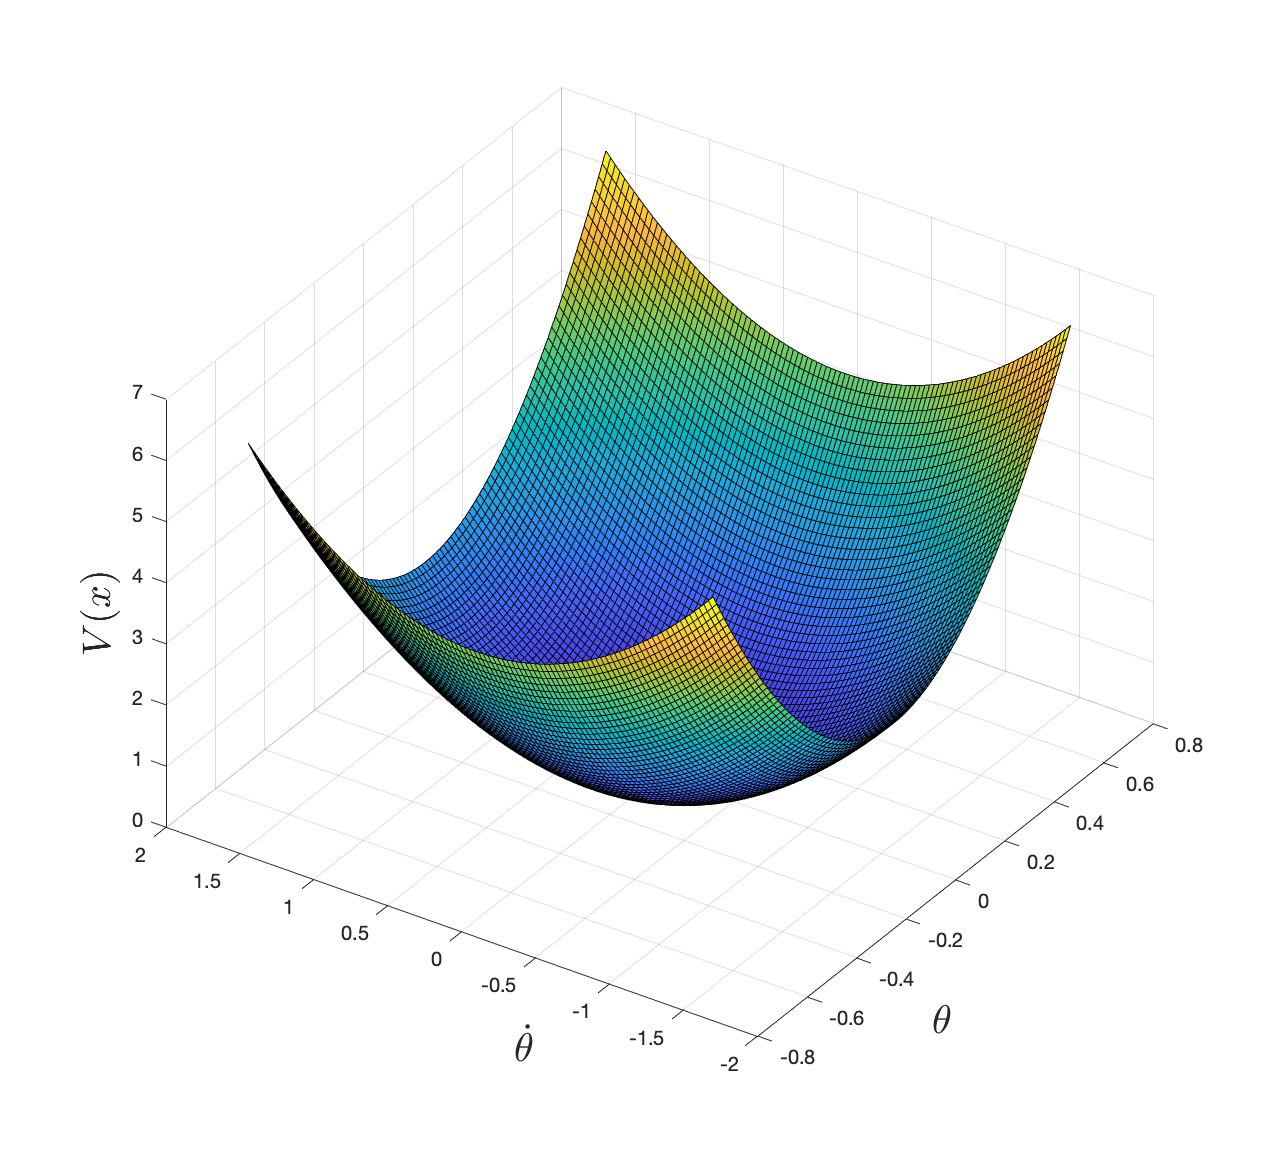
\includegraphics[width=0.6\linewidth]{images/pendulum-local-lyapunov-certificate-V} 

}

\caption{Lyapunov local stability certificate computed via convex optimization.}\label{fig:lyapunov-local-certificate-pendulum-V}
\end{figure}

and verify that \(V(x)\) is locally positive definite.

Plotting \(\dot{V}(x)\) in the constraint set \eqref{eq:lyapunovlocalstabilitypendulumsos-constraintset} using \((\theta, \dot{\theta})\) coordinates, we get

\begin{figure}

{\centering 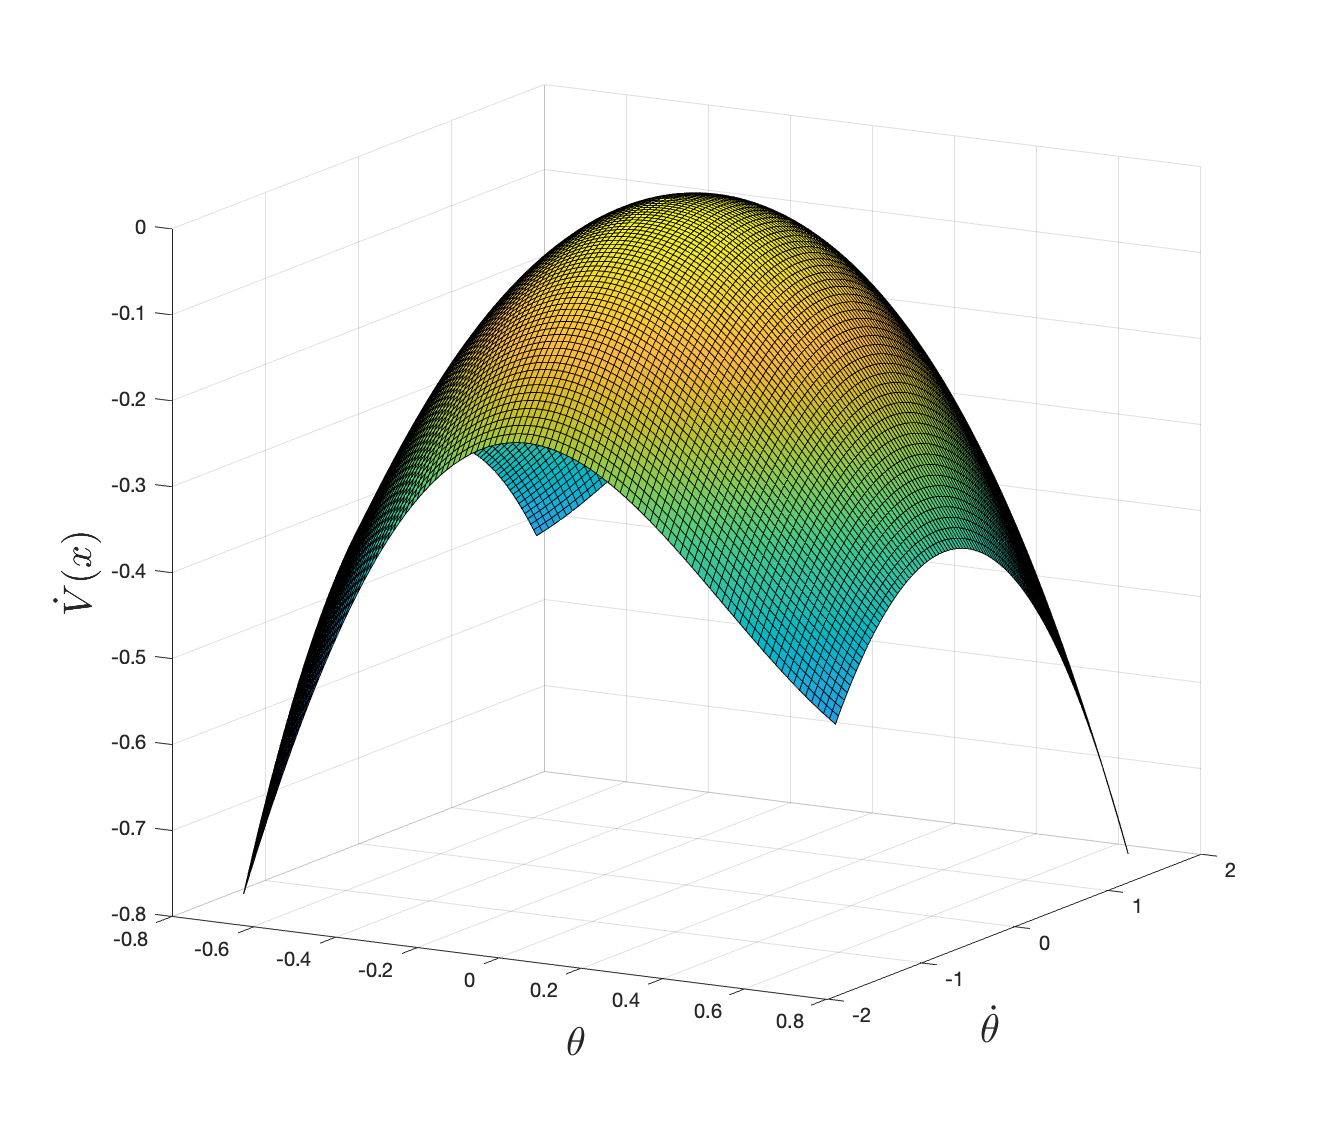
\includegraphics[width=0.6\linewidth]{images/pendulum-local-lyapunov-certificate-Vdot} 

}

\caption{Derivative of the Lyapunov local stability certificate computed via convex optimization.}\label{fig:lyapunov-local-certificate-pendulum-Vdot}
\end{figure}

and verify that \(\dot{V}(x)\) is locally negative definite.

You should try the code for this example \href{https://github.com/ComputationalRobotics/OptimalControlEstimation-Examples/blob/main/pendulum_local_lyapunov_certificate.m}{here}.
\end{example}

\hypertarget{controlled-systems}{%
\section{Controlled Systems}\label{controlled-systems}}

We can generalize the notion of a Lyapunov function for an autonomous system to the notion of a \emph{Control Lyapunov Function} (CLF) for a controlled system \citep{sontag83sicopt-clf}.

Consider a controlled system
\begin{equation}
\dot{x} = f(x,u)
\label{eq:clf-controlled-system}
\end{equation}
where \(x \in \mathbb{X} \subseteq \mathbb{R}^n\) the state, \(u \in \mathbb{U} \subseteq \mathbb{R}^m\) the control, and \(f\) is continuously differentiable. Let \(x = 0, u=0\) be an equilibrium point, i.e., \(f(0,0) = 0\). The existence of a CLF guarantees that we can design a controller to stabilize the equilibrium point.

\begin{theorem}[Control Lyapunov Function]
\protect\hypertarget{thm:control-lyapunov}{}\label{thm:control-lyapunov}Let \(V(x): \mathbb{X} \rightarrow \mathbb{R}\) be a continuously differentiable positive definite function, i.e., \(V(0) = 0\) and \(V(x) > 0, \forall x \in \mathbb{X} \backslash \{ 0 \}\). If there exists \(\rho > 0\) such that \(\Omega := \{ x \in \mathbb{X} \mid V(x) \leq \rho \}\) is bounded and
\begin{equation}
\min_{u \in \mathbb{U}} \dot{V}(x) = \frac{\partial V}{\partial x} f(x,u) < 0, \quad \forall x \in \Omega \backslash \{ 0 \},
\label{eq:clf-derivative-condition}
\end{equation}
then \(V(x)\) is called a control Lyapunov function.

In this case, if the system starts within the set \(\Omega\), then there exists a controller \(u(t)\) that drives the system towards the equilibrium point \(0\).
\end{theorem}

In Theorem \ref{thm:control-lyapunov}, it is clear that \(Omega\) is a control invariant set. In fact, \(Omega\) is an inner approximation of the \emph{region of attraction} to the equilibrium point \(0\).

\textbf{Deploying a CLF}. Now we observe that, when a CLF \(V(x)\) is given, it can help us design an asymptotically stablizing controller. Consider a special instance of the controlled system \eqref{eq:clf-controlled-system} that is \emph{control-affine}
\begin{equation}
\dot{x} = f_1(x) + f_2(x)u.
\label{eq:control-affine-system-clf}
\end{equation}
Clearly, the dynamics \eqref{eq:control-affine-system-clf} is affine in the control \(u\). Almost all robotics systems are control affine, so \eqref{eq:control-affine-system-clf} is quite general. Suppose we are given an arbitrary controller \(u_d(t)\), which may or may not stabilize the system towards the equilibrium point (e.g., \(u_d(t)\) may be obtained from neural networks). We can use the CLF \(V(x)\) to correct \(u_d(t)\) so that we always obtain a stabilizing feedback controller
\begin{equation}
\begin{split}
u(x(t)) = \arg\min_{u \in \mathbb{U}} & \quad \Vert u - u_d(t) \Vert^2 \\
\text{subject to} & \quad \dot{V}(x) = \frac{\partial V}{\partial x} (f_1(x) + f_2(x) u) < 0.
\end{split}
\label{eq:deploy-clf}
\end{equation}
Note that the optimization \eqref{eq:deploy-clf} is actually a convex optimization problem! Since we are minimizing over \(u\) (the state \(x(t)\) is given), the objective in \eqref{eq:deploy-clf} is quadratic in \(u\) and the constraint in \eqref{eq:deploy-clf} is linear in \(u\), implying \eqref{eq:deploy-clf} is a quadratic optimization problem. The CLF condition \eqref{eq:clf-derivative-condition} ensures that \eqref{eq:deploy-clf} is always feasible. Intuitively, optimization \eqref{eq:deploy-clf} seeks to find the feedback controller that (a) minimally modifies the given arbitrary controller \(u_d(t)\), and (b) guarantees stabilization towards the equilibrium.

\textbf{Verification and Synthesis of a CLF}. When a CLF is given, deploying it to compute a stablizing controller is easy. However, verifying if a candidate function is indeed a control Lyapunov function is a highly nontrivial task. In fact, it is an active area of research. The interested reader can refer to \citep{kang23cdc-verification} and \citep{dai23acc-convex}.

\hypertarget{non-autonomous-systems}{%
\section{Non-autonomous Systems}\label{non-autonomous-systems}}

\begin{lemma}[Barbalat's Lemma]
\protect\hypertarget{lem:Barbalat}{}\label{lem:Barbalat}Let \(f(t)\) be differentiable, if

\begin{itemize}
\item
  \(\lim_{t \rightarrow \infty} f(t)\) is finite, and
\item
  \(\dot{f}(t)\) is uniformly continuous,\footnote{A sufficient condition for this to hold is that \(\ddot{f}\) exists and is bounded.}
\end{itemize}

then
\[
\lim_{t \rightarrow \infty} \dot{f}(t) = 0.
\]
\end{lemma}

\begin{theorem}[Barbalat's Stability Certificate]
\protect\hypertarget{thm:BarbalatStability}{}\label{thm:BarbalatStability}If a scalar function \(V(x,t)\) satisfies

\begin{itemize}
\item
  \(V(x,t)\) is lower bounded,
\item
  \(\dot{V}(x,t)\) is negative semidefinite
\item
  \(\dot{V}(x,t)\) is uniformly continuous
\end{itemize}

then \(\dot{V}(x,t) \rightarrow 0\) as \(t \rightarrow \infty\).
\end{theorem}

\begin{proof}
\(V(x,t)\) is lower bounded and \(\dot{V}\) is negative semidefinite implies the limit of \(V\) as \(t \rightarrow \infty\) is finite (note that \(V(x,t) \leq V(x(0),0)\)). Then the theorem clearly follows from Barbalat's Lemma \ref{lem:Barbalat}.
\end{proof}

\hypertarget{output-feedback}{%
\chapter{Output Feedback}\label{output-feedback}}

We have presented many algorithms for optimal control of dynamical systems. These algorithms, however, have a strict assumption, i.e., the state of the system is directly available. These controllers are called \emph{state-feedback} controllers.

In many applications, the state of the system is not readily available but measured via sensors. Therefore, a more realistic model of the dynamical system is
\begin{equation}
\begin{split}
\dot{x} &= f(x,u) + w  \\
y &= h(x,u) + v
\end{split} 
\label{eq:output-feedback-system}
\end{equation}
where \(x(t) \in \mathbb{X} \subseteq \mathbb{R}^n\) the state of the system, \(u(t) \in \mathbb{U} \subseteq \mathbb{R}^m\) the control (or input), \(y(t) \in \mathbb{Y} \subseteq \mathbb{R}^{d}\) the output (i.e., measurement) of the state and control, and \(f,g\) the evolution and measurement functions (which are sufficiently smooth). \(w(t)\) and \(v(t)\) denote disturbance and measurement noise, respectively. The discrete-time analog of \eqref{eq:output-feedback-system} is
\begin{equation}
\begin{split}
x_{k+1} &= f(x_k,u_k) + w_k  \\
y_k &= h(x_k,u_k) + v_k
\end{split},
\label{eq:output-feedback-system-discrete-time}
\end{equation}
with \(k\) denoting the discrete timestep. When faced with systems like \eqref{eq:output-feedback-system} and \eqref{eq:output-feedback-system-discrete-time}, the controller typically needs to use the history of all measurements, also known as \emph{output feedback}
\[
u(t) = \pi(\{y(\tau)\}_{\tau=0}^t), \quad u_k = \pi (\{y_0,\dots,y_k\}).
\]

\hypertarget{least-squares-estimation}{%
\section{Least-Squares Estimation}\label{least-squares-estimation}}

Suppose we are given two random variables \(x \in \mathbb{R}^n\) and \(y \in \mathbb{R}^m\), where \(y\) is a measurement that provides some information about the model \(x\). We are interested in finding an \emph{estimator}, i.e., a function \(x(y)\), that minimizes
\[
\mathbb{E}_{x,y} \left\{ \Vert x - x(y) \Vert^2 \right\}.
\]
The optimal estimator, \(x^\star(y)\), is called a \emph{least-squares estimator}:
\[
x^\star(y) = \arg\min_{x(\cdot)} \mathbb{E}_{x,y} \left\{ \Vert x - x(y) \Vert^2 \right\}.
\]
Note that \(x^\star(y)\) is a function with input \(y\).
Since
\begin{equation}
\mathbb{E}_{x,y}\left\{ \Vert x - x(y) \Vert^2 \right\} = \mathbb{E}_y \left\{ \mathbb{E}_x \left\{ \Vert x - x(y) \Vert^2 \mid y\right\} \right\},
\label{eq:expand-conditional-expectation}
\end{equation}
it is clear that \(x^\star(y)\) is a least-squares estimator if \(x^\star(y)\) minimizes the conditional expectation in \eqref{eq:expand-conditional-expectation} for every \(y \in \mathbb{R}^m\), that is,
\begin{equation}
x^\star(y) = \arg\min_{z \in \mathbb{R}^n} \mathbb{E}_x \left\{ \Vert x - z \Vert^2 \mid y \right\}, \quad \forall y \in \mathbb{R}^m.
\label{eq:rewrite-least-squares-conditional}
\end{equation}
With this observation, we have the following proposition.

\begin{proposition}[Least Squares Estimator]
\protect\hypertarget{prp:least-squares-estimator}{}\label{prp:least-squares-estimator}The least squares estimator \(x^\star(y)\) is given by
\begin{equation}
x^\star(y) = \mathbb{E}_x \left\{ x \mid y \right\}, \quad \forall y \in \mathbb{R}^m,
\label{eq:conditional-mean}
\end{equation}
i.e., \(x^\star(y)\) returns the conditional mean of \(x\) given \(y\).
\end{proposition}

\begin{proof}
We expand the objective in \eqref{eq:rewrite-least-squares-conditional}
\[
\mathbb{E}_x \left\{ \Vert x - z \Vert^2 \mid y \right\} = \mathbb{E}_x \left\{ \Vert x \Vert^2 \mid y \right\} - 2 z^T \mathbb{E}_x \left\{x \mid y \right\} + \Vert z \Vert^2.
\]
Observe that problem \eqref{eq:rewrite-least-squares-conditional} is an unconstrained quadratic optimization, whose optimal solution can be obtained by setting the gradient of objective (w.r.t. \(z\)) to zero:
\[
z = \mathbb{E}_x \left\{ x \mid y \right\},
\]
concluding the proof.
\end{proof}

Depending on the joint distribution of \((x,y)\), the least-squares estimator can be very complicated (due to \(\mathbb{E}_x\left\{ x \mid y\right\}\) being complicated) and in general does not admit a clean solution. We now turn to the family of linear estimators.

\hypertarget{linear-least-squares-estimation}{%
\subsection{Linear Least-Squares Estimation}\label{linear-least-squares-estimation}}

A linear estimator \(x(y)\) takes the following form
\[
x(y) = Ay + b, \quad A \in \mathbb{R}^{n \times m}, b \in \mathbb{R}^n.
\]
The optimal linear estimator
\begin{equation}
(A^\star, b^\star) = \arg\min_{A,b} \mathbb{E}_{x,y} \left\{ \Vert x - Ay - b \Vert^2 \right\}
\label{eq:linear-least-squares-estimator}
\end{equation}
is called a \emph{linear least-squares estimator}.

In the special case where \(x\) and \(y\) are jointly Gaussian random variables, the conditional expectation \(\mathbb{E}_{x} \{x \mid y \}\) is indeed linear, and hence a linear least-squares estimator is also the true least-squares estimator.

\begin{proposition}[Linear Least-Squares Estimator]
\protect\hypertarget{prp:linear-least-squares-estimator}{}\label{prp:linear-least-squares-estimator}If the random variables \((x,y)\) are jointly Gaussian, then the conditional expectation \(\mathbb{E}_x \{x \mid y \}\) is linear in \(y\). Therefore, the linear least-squares estimator \eqref{eq:linear-least-squares-estimator} is also the least-squares estimator.
\end{proposition}

Now let us turn to characterize the linear least-squares estimator.

\begin{proposition}[Solution of Linear Least-Squares Estimator]
\protect\hypertarget{prp:linear-least-squares-solution}{}\label{prp:linear-least-squares-solution}Let \(x,y\) be random variables in \(\mathbb{R}^n\) and \(\mathbb{R}^m\) drawn from some underlying distribution. The means and covariances of \(x\) and \(y\) are given by
\begin{equation}
\begin{split}
\mathbb{E}\{ x\} = \bar{x}, \quad \mathbb{E} \{ y \} = \bar{y}. \\
\mathbb{E}\{ (x - \bar{x})(x - \bar{x})^T \} = \Sigma_{xx}, \quad \mathbb{E}\{ (y - \bar{y})(y-\bar{y})^T \} = \Sigma_{yy}, \\
\mathbb{E}\{ (x - \bar{x})(y - \bar{y})^T \} = \Sigma_{xy}, \quad \mathbb{E}\{ (y - \bar{y})(x - \bar{x})^T \} = \Sigma^T_{xy},
\end{split}
\end{equation}
and assume \(\Sigma_{yy}\) is invertible (positive definite). Then the linear least-squares estimator \(x^\star(y)\), i.e., solution of \eqref{eq:linear-least-squares-estimator}, is given by
\begin{equation}
x^\star(y) = \bar{x} + \Sigma_{xy} \Sigma^{-1}_{yy} (y - \bar{y}).
\label{eq:linear-least-squares-solution}
\end{equation}
The corresponding error covariance matrix is given by
\begin{equation}
\mathbb{E}_{x,y} \left\{ (x - x^\star(y))(x - x^\star(y))^T \right\} = \Sigma_{xx} - \Sigma_{xy} \Sigma^{-1}_{yy} \Sigma^T_{xy}.
\label{eq:linear-least-squares-solution-covariance}
\end{equation}
\end{proposition}

\begin{proof}
Problem \eqref{eq:linear-least-squares-estimator} is an unconstrained quadratic optimization in \((A,b)\). Therefore, its optimal solution can be computed by taking the derivative of the objective, i.e., \(f(A,b) = \mathbb{E}_{x,y} \{ \Vert x - Ay - b \Vert^2 \}\) , w.r.t. \((A,b)\) and setting them to zero
\begin{equation}
\begin{split}
0 = \frac{\partial f}{\partial A} = 2 \mathbb{E}_{x,y} \{ (b + Ay -x) y^T \}, \\
0 = \frac{\partial f}{\partial b} = 2 \mathbb{E}_{x,y} \{ b + Ay - x \}.
\end{split}
\label{eq:linear-least-squares-derivative-zero}
\end{equation}
The second equation gives us the solution of \(b^\star\)
\begin{equation}
b^\star = \bar{x} - A \bar{y}.
\label{eq:linear-least-squares-proof-solution-b}
\end{equation}
Plug the solution \eqref{eq:linear-least-squares-proof-solution-b} back into the first equation in \eqref{eq:linear-least-squares-derivative-zero}, we obtain
\begin{equation}
\mathbb{E}_{x,y} \{ (A(y - \bar{y}) - (x - \bar{x})) y^T\} = 0.
\label{eq:linear-least-squares-proof-simplify-first-equation}
\end{equation}
On the other hand, we have
\begin{equation}
\left( \mathbb{E}_{x,y} \{ A (y - \bar{y}) - (x - \bar{x})\} \right) \bar{y}^T = 0.
\label{eq:linear-least-squares-proof-simplify-first-equation-other}
\end{equation}
Subtracting \eqref{eq:linear-least-squares-proof-simplify-first-equation-other} from \eqref{eq:linear-least-squares-proof-simplify-first-equation}, we have
\[
\mathbb{E}_{x,y} \left\{ (A(y-\bar{y}) - (x - \bar{x})) (y - \bar{y})^T \right\} = 0,
\]
which is exactly
\[
A \Sigma_{yy} - \Sigma_{xy} = 0.
\]
Therefore, we obtain the optimal \(A\)
\begin{equation}
A^\star = \Sigma_{xy} \Sigma^{-1}_{yy}.
\label{eq:linear-least-squares-proof-solution-A}
\end{equation}
Combining \eqref{eq:linear-least-squares-proof-solution-A} and \eqref{eq:linear-least-squares-proof-solution-b}, we get the optimal linear least-squares estimator
\[
x^\star(y) = \Sigma_{xy} \Sigma^{-1}_{yy} y + \left( \bar{x} -  \Sigma_{xy} \Sigma^{-1}_{yy} \bar{y} \right) = \bar{x} + \Sigma_{xy} \Sigma^{-1}_{yy} (y - \bar{y}).
\]
The error covariance \eqref{eq:linear-least-squares-solution-covariance} follows by direct computation.
\end{proof}

We next list a few useful properties of the linear least-squares estimator.

\begin{corollary}[Properties of the Linear Least-Squares Estimator]
\protect\hypertarget{cor:properties-linear-least-squares-estimator}{}\label{cor:properties-linear-least-squares-estimator}The linear least-squares estimator \(x^\star(y)\) in \eqref{eq:linear-least-squares-solution} is unbiased, i.e.,
\[
\mathbb{E}_y \{ x^\star(y) \} = \bar{x}.
\]

The estimation error \(x - x^\star(y)\) is uncorrelated with both \(y\) and \(x^\star(y)\), i.e.,
\begin{equation}
\begin{split}
\mathbb{E}_{x,y} \{  (x - x^\star(y))y^T \} = 0. \\
\mathbb{E}_{x,y} \{  (x - x^\star(y)) (x^\star(y))^T \} = 0.
\end{split}
\label{eq:linear-least-squares-orthogonal-projection}
\end{equation}
\end{corollary}

Equation \eqref{eq:linear-least-squares-orthogonal-projection} is known as the \emph{orthogonal projection principle}.

The next corollary considers the linear least-squares estimator of a new variable \(z\) that is a linear function of \(x\).

\begin{corollary}
\protect\hypertarget{cor:linear-least-squares-z}{}\label{cor:linear-least-squares-z}Consider in addition to \(x\) and \(y\), the random vector \(z\) defined by
\[
z = Cx,
\]
where \(C \in \mathbb{R}^{p \times n}\) is given. Then the linear least-squares estimator of \(z\) given \(y\) is
\[
z^\star(y) = C x^\star(y),
\]
and the corresponding error covariance matrix is
\[
\mathbb{E}_{z,y}\left\{ (z - z^\star(y))(z - z^\star(y))^T \right\} = C \mathbb{E}_{x,y} \left\{ (x - x^\star(y))(x - x^\star(y))^T \right\} C^T,
\]
where \(\mathbb{E}_{x,y} \left\{ (x - x^\star(y))(x - x^\star(y))^T \right\}\) is given in \eqref{eq:linear-least-squares-solution-covariance}.
\end{corollary}

\begin{proof}
Since \(z = Cx\), we have \(\mathbb{E} \{ z \} = C \bar{x} = \bar{z}\), and
\[
\Sigma_{zz} = \mathbb{E} \{ (z - \bar{z})(z - \bar{z})^T \} = C \Sigma_{xx} C^T, \\
\Sigma_{zy} = \mathbb{E} \{ (z - \bar{z})(y - \bar{y})^T \} = C \Sigma_{xy}, \\
\Sigma_{yz} = \mathbb{E} \{ (y - \bar{y}) (z - \bar{z})^T \} = \Sigma^T_{xy} C^T.
\]
The result then follows by applying Proposition \ref{prp:linear-least-squares-solution} to \(z\) and \(y\).
\end{proof}

The next corollary considers the linear least-squares estimator of \(x\) given \(z\), a random vector that is a linear function of \(y\).

\begin{corollary}
\protect\hypertarget{cor:linear-least-squares-x-z}{}\label{cor:linear-least-squares-x-z}Consider in addition to \(x\) and \(y\), an additional random variable \(z\)
\[
z = C y + u,
\]
where \(C \in \mathbb{R}^{p \times m}\), with rank \(p\), and \(u \in \mathbb{R}^p\) are given. Then the linear least-squares estimator of \(x\) given \(z\) is
\[
x^\star(z) = \bar{x} + \Sigma_{xy} C^T (C \Sigma_{yy} C^T)^{-1} (z - C \bar{y} - u),
\]
and the corresponding error covariance matrix is
\[
\mathbb{E}_{x,z}\left\{ (x - x^\star(z))(x - x^\star(z))^T \right\} = \Sigma_{xx} - \Sigma_{xy} C^T (C \Sigma_{yy} C^T)^{-1} C \Sigma_{xy}^T.
\]
\end{corollary}

\begin{proof}
Since \(z = Cy + u\), we have \(\bar{z} = \mathbb{E}\{ z \} = C \bar{y} + u\), and
\[
\Sigma_{zz} = \mathbb{E}\{ (z - \bar{z})(z - \bar{z})^T \} = C \Sigma_{yy} C^T, \\
\Sigma_{zx} = \mathbb{E}\{ (z - \bar{z})(x - \bar{x})^T \} = C \Sigma_{xy}^T, \\
\Sigma_{xz} = \mathbb{E}\{ (x - \bar{x})(z - \bar{z})^T \} = \Sigma_{xy}C^T.
\]
The result then follows by applying Proposition \ref{prp:linear-least-squares-solution}.
\end{proof}

Frequently, we want to estimate a vector of parameters \(x \in \mathbb{R}^n\) given a measurement vector \(z \in \mathbb{R}^m\) of the form \(z = C x + v\) with \(C \in \mathbb{R}^{m \times n}\) a given matrix and \(v \in \mathbb{R}^m\) a noise vector. The following corollary gives the linear least squares estimator \(x^\star(z)\) and its error covariance.

\begin{corollary}[Linear Least-Squares Estimator with Noise]
\protect\hypertarget{cor:linear-least-squares-noise}{}\label{cor:linear-least-squares-noise}Let
\[
z = C x + v,
\]
where \(C \in \mathbb{R}^{m \times n}\) is a given matrix, and the random variable \(x\) and \(v\) are uncorrelated. Denote
\[
\mathbb{E}\{x \} = \bar{x}, \quad \mathbb{E}\{ (x - \bar{x})(x - \bar{x})^T \} = \Sigma_{xx}, \\
\mathbb{E}\{ v\} = \bar{v}, \quad \mathbb{E}\{ (v - \bar{v})(v - \bar{v})^T \} = \Sigma_{vv},
\]
and assume \(\Sigma_{vv}\) is positive definite. Then the linear least-squares estimator of \(x\) given \(z\) is
\[
x^\star(z) = \bar{x} + \Sigma_{xx} C^T (C \Sigma_{xx} C^T + \Sigma_{vv})^{-1} (z - C \bar{x} - \bar{v}),
\]
and the corresponding error covariance is
\[
\mathbb{E}_{x,v} \{ (x - x^\star(z))(x - x^\star(z))^T \} = \Sigma_{xx} - \Sigma_{xx}C^T (C \Sigma_{xx} C^T + \Sigma_{vv})^{-1} C \Sigma_{xx}.
\]
\end{corollary}

\begin{proof}
Denote
\[
y = \begin{bmatrix} x \\ v \end{bmatrix}, \quad \bar{y} = \begin{bmatrix} \bar{x} \\ \bar{v} \end{bmatrix},
\]
then clearly we have
\[
x = \underbrace{ \begin{bmatrix} I & 0 \end{bmatrix}}_{C_x} y,
\]
and
\[
z = \underbrace{\begin{bmatrix} C & I \end{bmatrix}}_{\tilde{C}} y.
\]
Using Corollary \ref{cor:linear-least-squares-z}, we have
\[
x^\star(z) = C_x y^\star(z) \\
\mathbb{E}\{ (x - x^\star(z))(x - x^\star(z))^T \} = C_x \mathbb{E}\{(y - y^\star(z))(y - y^\star(z))^T \} C_x^T,
\]
where \(y^\star(z)\) is the linear least-sqaures estimator of \(y\) given \(z\).

To obtain \(y^\star(z)\), we can apply Corollary \ref{cor:linear-least-squares-x-z} with \(u=0\) and \(x=y\), leading to
\[
y^\star(z) = \bar{y} + \Sigma_{yy} \tilde{C}^T (\tilde{C} \Sigma_{yy} \tilde{C}^T)^{-1} (z - \tilde{C}\bar{y}),
\]
and the error covariance
\[
\mathbb{E}\{(y - y^\star(z))(y - y^\star(z))^T \} = \Sigma_{yy} - \Sigma_{yy} \tilde{C}^T (\tilde{C}\Sigma_{yy}\tilde{C}^T)^{-1} \tilde{C} \Sigma_{yy}.
\]
The result then follows by noting
\[
\Sigma_{yy} = \begin{bmatrix} \Sigma_{xx} & 0 \\ 0 & \Sigma_{vv} \end{bmatrix}
\]
because \(x\) and \(v\) are uncorrelated.
\end{proof}

The next two corollaries deal with least-squares estimators involving multiple measurements arriving sequentially. In particular, the corollaries show how to modify an existing least-squares estimate \(x^\star(y)\) to obtain \(x^\star(y,z)\) once an additional measurement \(z\) becomes available. This is a central operation in Kalman filtering.

\begin{corollary}[Linear Least-Squares Estimator of Uncorrelated Measurements]
\protect\hypertarget{cor:linear-least-squares-correction-uncorrelated}{}\label{cor:linear-least-squares-correction-uncorrelated}Consider in addition to \(x\) and \(y\), an additional random vector \(z \in \mathbb{R}^p\) that is uncorrelated with \(y\). Then the linear least-squares estimator \(x^\star(y,z)\) of \(x\) given both \(y\) and \(z\) has the form
\[
x^\star(y,z) = x^\star(y) + x^\star(z) - \bar{x},
\]
where \(x^\star(y)\) and \(x^\star(z)\) are the linear least-squares estimates of \(x\) given \(y\) and given \(z\), respectively. Furthermore, the error covariance matrix is
\[
\mathbb{E}_{x,y,z} \{ (x - x^\star(y,z))(x - x^\star(y,z))^T \} = \Sigma_{xx} - \Sigma_{xy} \Sigma^{-1}_{yy} \Sigma^T_{xy} - \Sigma_{xz} \Sigma^{-1}_{zz} \Sigma_{xz}^T,
\]
where
\[
\Sigma_{xz} = \mathbb{E}_{x,z}\{ (x - \bar{x})(z - \bar{z})^T \}, \quad \Sigma_{zz} = \mathbb{E}_{z} \{ (z - \bar{z})(z - \bar{z})^T \}, \quad \bar{z} = \mathbb{E}_z \{ z \},
\]
and it is assumed that \(\Sigma_{zz}\) and \(\Sigma_{yy}\) are both invertible.
\end{corollary}

\begin{proof}
Let
\[
w = \begin{bmatrix} y \\ z \end{bmatrix}, \quad \bar{w} = \begin{bmatrix} \bar{y} \\ \bar{z} \end{bmatrix}.
\]
Then we can apply Proposition \ref{prp:linear-least-squares-solution} to compute the linear least-squares estimator of \(x\) given \(w\)
\[
x^\star(w) = \bar{x} + \Sigma_{xw} \Sigma^{-1}_{ww} (w - \bar{w}).
\]
On the other hand, we have
\[
\Sigma_{xw} = \mathbb{E}\{ (x - \bar{x}) \begin{bmatrix} (y - \bar{y})^T & ( z - \bar{z} )^T \end{bmatrix} \} = \begin{bmatrix} \Sigma_{xy} & \Sigma_{xz} \end{bmatrix},
\]
and since \(y\) and \(z\) are uncorrelated, we have
\[
\Sigma_{ww} = \begin{bmatrix} \Sigma_{yy} & 0 \\ 0 & \Sigma_{zz} \end{bmatrix}.
\]
The result then follows by direct computation.
\end{proof}

The next corollary generalizes the previous result to the case where \(y\) and \(z\) are correlated.

\begin{corollary}[Linear Least-Squares Estimator of Correlated Measurements]
\protect\hypertarget{cor:linear-least-squares-correction-correlated}{}\label{cor:linear-least-squares-correction-correlated}Consider the situation in Corollary \ref{cor:linear-least-squares-correction-uncorrelated}, but with \(z\) and \(y\) being correlated
\[
\Sigma_{yz} = \mathbb{E}_{y,z} \{ (y - \bar{y})(z - \bar{z})^T \} \neq 0.
\]
Then \(x^\star(y,z)\) has the following form
\[
x^\star(y,z) = x^\star(y) + x^\star(z - z^\star(y)) - \bar{x},
\]
where \(x^\star(z - z^\star(y))\) denotes the linear least-squares estimate of \(x\) given the random vector \(z - z^\star(y)\) and \(z^\star(y)\) is the linear least-squares estimate of \(z\) given \(y\). Furthermore, the error covariance matrix is
\[
\mathbb{E}_{x,y,z} \{ (x - x^\star(y,z))(x - x^\star(y,z))^T \} = \Sigma_{xx} - \Sigma_{xy} \Sigma^{-1}_{yy} \Sigma^T_{xy} - \hat{\Sigma}_{xz} \hat{\Sigma}^{-1}_{zz} \hat{\Sigma}^T_{xz},
\]
where
\[
\hat{\Sigma}_{xz} = \mathbb{E}_{x,y,z} \{ (x - \bar{x})(z - z^\star(y))^T \}, \quad \hat{\Sigma}_{zz} = \mathbb{E}_{y,z} \{ (z - z^\star(y))(z - z^\star(y))^T \}.
\]
\end{corollary}

\begin{proof}
By Proposition \ref{prp:linear-least-squares-solution}, we know \(z^\star(y)\) is linear in \(y\) as
\[
z^\star(y) = \bar{z} + \Sigma_{zy} \Sigma^{-1}_{yy} (y - \bar{y}) := B y + c,
\]
where \(B = \Sigma_{zy} \Sigma^{-1}_{yy}\) and \(c = \bar{z} - \Sigma_{zy} \Sigma^{-1}_{yy} \bar{y}\). The linear least-squares estimate of \(x\) given \((y,z)\) has the form
\begin{equation}
x = \begin{bmatrix} A_y^\star & A_z^\star \end{bmatrix} \begin{bmatrix} y \\ z \end{bmatrix} + b^\star,
\label{eq:linear-least-squares-solution-A-b}
\end{equation}
where \((A_y^\star, A_z^\star, b^\star)\) is solution to
\begin{equation}
(A_y^\star, A_z^\star, b^\star) = \arg\min_{A_y,A_z,b} \mathbb{E}_{x,y,z} \left\{ \Vert x - A_y y - A_z z - b  \Vert^2 \right\}.
\label{eq:correlated-A-b}
\end{equation}
The linear least-squares estimate of \(x\) given \((y, z - z^\star(y))\) has the form
\begin{equation}
x = \begin{bmatrix} G_y^\star & G_z^\star \end{bmatrix} \begin{bmatrix} y \\ z - By - c \end{bmatrix} + h^\star,
\label{eq:linear-least-squares-solution-G-h}
\end{equation}
where \((G_y^\star,G_z^\star,h^\star)\) is solution to
\begin{equation}
(G_y^\star,G_z^\star,h^\star) = \arg\min_{G_y,G_z,h} \mathbb{E}_{x,y,z} \left\{ \Vert x - G_y y - G_z (z - By - c) - h \Vert^2 \right\}.
\label{eq:correlated-G-h}
\end{equation}
Observe that the objective in \eqref{eq:correlated-G-h} can be rewritten as
\[
\mathbb{E}_{x,y,z} \left\{ \Vert x - (G_y - G_z B) y - G_z z - (h - G_z c) \Vert^2 \right\},
\]
when matched with the objective of \eqref{eq:correlated-A-b} we have
\[
A_y^\star = G_y^\star - G_z^\star B, \quad  A_z^\star = G_z^\star, \quad b^\star = h^\star - G_z^\star c.
\]
As a result, the linear least-squares estimator in \eqref{eq:linear-least-squares-solution-G-h} becomes
\[
x = (A_y^\star + A_z^\star B) y + A_z^\star (z - By - c) + b^\star + A_z^\star c = A^\star_y y + A^\star_z z + b^\star,
\]
which is the same as \eqref{eq:linear-least-squares-solution-A-b}. Therefore, we have
\[
x^\star(y,z) = x^\star(y, z - z^\star(y)).
\]

From Corollary \ref{cor:properties-linear-least-squares-estimator}, we know \(y\) and \(z - z^\star(y)\) is uncorrelated. Consequently, we reduce to the uncorrelated setup in Corollary \ref{cor:linear-least-squares-correction-uncorrelated} and the result follows.
\end{proof}

\hypertarget{kalman-filter}{%
\section{Kalman Filter}\label{kalman-filter}}

Consider now a linear dynamical system without control
\begin{equation}
\begin{cases}
x_{k+1} = A_k x_k + w_k \\
y_k = C_k x_k + v_k
\end{cases}, k=0,1,\dots,N-1,
\label{eq:kalman-filter-linear-system-discrete}
\end{equation}
where \(x_k \in \mathbb{R}^n\) the state, \(w_k \in \mathbb{R}^n\) the random disturbance, \(y_k \in \mathbb{R}^d\) the measurement (output), and \(v_k \in \mathbb{R}^d\) the measurement noise.

We assume \(x_0,w_0,\dots,w_{N-1},v_0,\dots,v_{N-1}\) are independent random vectors with means
\[
\mathbb{E}\{ w_k \} = \mathbb{E} \{ v_k \} = 0, \quad k=0,\dots,N-1,
\]
and covariances
\[
\mathbb{E} \{ w_k w_k^T \} = M_k, \quad \mathbb{E} \{ v_k v_k^T \} = N_k, \quad k=0,\dots,N-1,
\]
with \(N_k\) positive definite for all \(k\). We assume the initial state \(x_0\) has mean \(\mathbb{E}\{ x_0 \}\) and covariance
\[
S = \mathbb{E} \{ (x_0 - \mathbb{E}\{x_0 \} ) (x_0 - \mathbb{E}\{x_0 \} )^T \}.
\]
Let
\[
Y_k = (y_0,\dots,y_k)
\]
be the set of measurements up to time \(k\), our goal is to obtain the linear least-squares estimate of \(x_k\) given \(Y_k\), denoted as
\[
x^\star_{k \mid k} := x^\star_k (Y_k),
\]
and its error covariance matrix
\[
\Sigma_{k \mid k} := \mathbb{E} \{ (x_k - x^\star_{k \mid k}) (x_k - x^\star_{k \mid k})^T\}.
\]
By definition, we have
\begin{equation}
x^\star_{0 \mid -1} = \mathbb{E}\{ x_0 \}, \quad \Sigma_{0 \mid -1} = S.
\label{eq:kalman-filter-initial-condition}
\end{equation}

The Kalman filter \citep{kalman60new} will derive a recursion to update \(x^\star_{k \mid k}\) and \(\Sigma_{k \mid k}\).

\textbf{Road map}. Towards this, let us assume we have computed \(x^\star_{k \mid k-1}\) and its error covariance \(\Sigma_{k \mid k-1}\) (the initial condition is given by \eqref{eq:kalman-filter-initial-condition}). Our goal is to compute \(x^\star_{k+1 \mid k}\) and its error covariance \(\Sigma_{k+1\mid k}\). We will see that, to compute \(x^\star_{k+1 \mid k}\), we compute \(x^\star_{k \mid k}\) first, and to compute \(\Sigma_{k+1 \mid k}\), we compute \(\Sigma_{k\mid k}\) first, as illustrated below.
\begin{equation}
\begin{split}
\text{Update estimate:}\quad x^\star_{k \mid k-1} \longrightarrow x^\star_{k \mid k} \longrightarrow x^\star_{k+1 \mid k}. \\
\text{Update covariance:}\quad \Sigma_{k \mid k-1} \longrightarrow \Sigma_{k \mid k} \longrightarrow \Sigma_{k+1 \mid k}.
\end{split}
\end{equation}

\textbf{Using the measurement}. At time \(k\), we receive a new measurement
\[
y_k = C_k x_k + v_k.
\]
We have
\[
x^\star_{k\mid k} = x^\star_k (Y_k) = x^\star_k(Y_{k-1},y_k),
\]
by Corollary \ref{cor:linear-least-squares-correction-correlated}, we have
\begin{equation}
x^\star_{k \mid k} = x^\star_{k \mid k-1} + x^\star_k (y_k - y_k^\star(Y_{k-1})) - \mathbb{E}\{ x_k \},
\label{eq:kalman-filter-derivation-1}
\end{equation}
where \(y_k^\star(Y_{k-1})\) is the linear least-squares estimate of \(y_k\) given \(Y_{k-1}\).

\textbf{Simplify \eqref{eq:kalman-filter-derivation-1}}. First note that by Corollary \ref{cor:linear-least-squares-z} and independence of \(v_k\), we have
\[
y_k^\star(Y_{k-1}) = C_k x^\star_{k \mid k-1}.
\]
We now need to compute \(x_k^\star(y_k - y_k^\star(Y_{k-1}))\). We do so by Proposition \ref{prp:linear-least-squares-solution}. The covariance matrix of \(y_k - y_k^\star(Y_{k-1})\) is, by Corollary \ref{cor:linear-least-squares-z},
\[
\mathbb{E} \{ (y_k - y_k^\star(Y_{k-1}))(y_k - y_k^\star(Y_{k-1}))^T \} = C_k \Sigma_{k \mid k-1} C_k^T + N_k.
\]
The correlation between \(x_k\) and \(y_k - y_k^\star(Y_{k-1})\) is
\begin{equation}
\begin{split}
\mathbb{E}\{ x_k (y_k - y_k^\star(Y_{k-1}))^T \} = \mathbb{E} \{ x_k(C_k (x_k - x^\star_{k\mid k-1}))^T \} + \underbrace{ \mathbb{E}\{ x_k v_k^T \} }_{=0 \text{ by independence of } v_k} \\
= \mathbb{E}\{(x_k - x^\star_{k \mid k-1}) (x_k - x^\star_{k \mid k-1})^T \}C_k^T + \underbrace{\mathbb{E}\{ x^\star_{k \mid k-1}(x_k - x^\star_{k \mid k-1})^T \}}_{=0 \text{ by the orthogonal projection principle}}C_k^T \\
= \Sigma_{k \mid k-1} C_k^T.
\end{split}
\end{equation}
As a result, by Proposition \ref{prp:linear-least-squares-solution}, we have
\[
x_k^\star(y_k - y_k^\star(Y_{k-1})) = \mathbb{E}\{x_k \} + \Sigma_{k \mid k-1} C_k^T (C_k \Sigma_{k \mid k-1} C_k^T + N_k)^{-1} (y_k - C_k x^\star_{k \mid k-1}).
\]

\textbf{Update the estimate}. Thus, \eqref{eq:kalman-filter-derivation-1} is simplified as
\begin{equation}
x^\star_{k\mid k} = x^\star_{k \mid k-1} + \Sigma_{k \mid k-1} C_k^T (C_k \Sigma_{k \mid k-1} C_k^T + N_k)^{-1} (y_k - C_k x^\star_{k \mid k-1}),
\label{eq:kalman-filter-update-1}
\end{equation}
which describes the update from \(x^\star_{k \mid k-1}\) to \(x^\star_{k \mid k}\).

To update \(x^\star_{k+1 \mid k}\) from \(x^\star_{k \mid k}\), by Corollary \ref{cor:linear-least-squares-z}, we have
\begin{equation}
x^\star_{k+1 \mid k} = A_k x^\star_{k \mid k}.
\label{eq:kalman-filter-update-2}
\end{equation}

\textbf{Update the covariance}. The error covariance \(\Sigma_{k \mid k}\), by Corollary \ref{cor:linear-least-squares-correction-correlated}, can be written as
\begin{equation}
\Sigma_{k \mid k} = \Sigma_{k \mid k-1} - \Sigma_{k\mid k-1} C_k^T (C_k \Sigma_{k \mid k-1} C_k^T + N_k)^{-1} C_k \Sigma_{k \mid k-1}.
\label{eq:kalman-filter-update-3}
\end{equation}
(This requires just a little bit thinking.) To update \(\Sigma_{k+1 \mid k}\) from \(\Sigma_{k \mid k}\), we can use Corollary \ref{cor:linear-least-squares-z} and the independence of \(w_k\) to obtain
\begin{equation}
\Sigma_{k+1 \mid k} = A_k \Sigma_{k \mid k} A_k^T + M_k.
\label{eq:kalman-filter-update-4}
\end{equation}

Equations \eqref{eq:kalman-filter-update-1}-\eqref{eq:kalman-filter-update-4} forms the Kalman Filter.

\textbf{Including controls}. When the dynamics includes control
\[
x_{k+1} = A_k x_k + B_k u_k + w_k,
\]
the only change that needs to be made to the Kalman Filter is that \eqref{eq:kalman-filter-update-2} should be replaced by
\begin{equation}
x^\star_{k+1 \mid k} = A_k x^\star_{k \mid k} + B_k u_k.
\label{eq:kalman-filter-update-5}
\end{equation}

\hypertarget{steady-state-kalman-filter}{%
\subsection{Steady-State Kalman Filter}\label{steady-state-kalman-filter}}

Combining the two updates on covariance matrices \eqref{eq:kalman-filter-update-3} and \eqref{eq:kalman-filter-update-4}, we obtain
\begin{equation}
\Sigma_{k+1 \mid k} = A_k (\Sigma_{k \mid k-1} - \Sigma_{k \mid k-1} C_k^T (C_k \Sigma_{k \mid k-1} C_k^T + N_k)^{-1} C_k \Sigma_{k \mid k-1}  ) A_k^T + M_k,
\label{eq:kalman-filter-covariance-recursion}
\end{equation}
which is the same as the discrete-time Riccati equation \eqref{eq:finite-discrete-lqr-riccati} when we study the solution of the finite-horizon LQR problem in Proposition \ref{prp:discretetimefinitehorizonlqrsolution}.

When \(A_k, C_k, M_k, N_k\) are constant matrices
\[
A_k = A, \quad C_k = C, \quad, M_k = M, \quad N_k = N,
\]
the recursion \eqref{eq:kalman-filter-covariance-recursion} tends to the algebraic Riccati equation
\begin{equation}
\Sigma = A(\Sigma - \Sigma C^T(C \Sigma C^T + N)^{-1}C \Sigma)A^T + M,
\label{eq:kalman-filter-algebraic-riccati-equation}
\end{equation}
for which a unique positive definite solution \(\Sigma\) exists if \((A,C)\) is observable and \((A,D)\) is controllable with \(M = D D^T\). Then, using equation \eqref{eq:kalman-filter-update-3}, we have that \(\Sigma_{k \mid k}\) tends to
\[
\bar{\Sigma} = \Sigma - \Sigma C^T (C \Sigma C^T + N)^{-1} C \Sigma.
\]
This leads to the simple steady-state Kalman filter
\begin{equation}
x^\star_{k \mid k} = \underbrace{A x^\star_{k-1 \mid k-1}}_{\text{prediction}} + \underbrace{\Sigma C^T(C \Sigma C^T + N)^{-1} (y_k - CA x_{k-1 \mid k-1})}_{\text{feedback correction}}.
\label{eq:steady-state-kalman-filter}
\end{equation}

\hypertarget{continuous-time-kalman-filter}{%
\subsection{Continuous-time Kalman Filter}\label{continuous-time-kalman-filter}}

Consider the continuous-time analog of the linear system in \eqref{eq:kalman-filter-linear-system-discrete}
\begin{equation}
\begin{cases}
\dot{x} = A x + Bu + w \\
y = C x + v
\end{cases}
\label{eq:kalman-filter-linear-system-continuous}
\end{equation}
where \(x \in \mathbb{R}^n\) the state, \(u \in \mathbb{R}^m\) the control, \(y \in \mathbb{R}^d\) the measurement, and \(w,v\) are white noises with
\[
\mathbb{E}\{w\}=0, \quad \mathbb{E}\{ w w^T \} = M, \quad \mathbb{E}\{v\} = 0, \quad  \mathbb{E}\{ v v^T\} = N.
\]

Suppose the initial state \(x(0)\) satisfies
\[
\mathbb{E}\{ x(0) \} = \hat{x}_0, \quad \mathbb{E}\{ (x(0) - \hat{x}_0) (x(0) - \hat{x}_0)^T \} = \Sigma_0.
\]
Then the continuous-time Kalman Filter updates the state estimate as
\begin{equation}
\dot{\hat{x}} = \underbrace{A \hat{x} + Bu}_{\text{prediction}} + \underbrace{K (y - C \hat{x})}_{\text{feedback correction}},
\label{eq:continuous-time-kalman-filter-state}
\end{equation}
where \(K\) is a feedback gain computed by
\[
K = \Sigma C^T N^{-1},
\]
with \(\Sigma\) satisfying the following differential equation
\begin{equation}
\dot{\Sigma} = A \Sigma + \Sigma A^T + M - \Sigma C^T N^{-1} C \Sigma.
\label{eq:continuous-time-kalman-filter-covariance}
\end{equation}
Similarly, at steady state, the differential equation \eqref{eq:continuous-time-kalman-filter-covariance} tends to the continuous-time algebraic Riccati equation
\[
0 = A \Sigma + \Sigma A^T + M - \Sigma C^T N^{-1} C \Sigma.
\]

\hypertarget{linear-quadratic-gaussian-control}{%
\section{Linear Quadratic Gaussian Control}\label{linear-quadratic-gaussian-control}}

With our knowledge about the Kalman filter, we are ready to solve a particular instance of output-feedback control, known as the Linear Quadratic Gaussian (LQG) control.

Consider the discrete-time linear dynamical system:
\begin{equation}
\begin{cases}
x_{k+1} = A_k x_k + B_k u_k + w_k \\
y_k = C_k x_k + v_k
\end{cases}, \quad k=0,\dots,N-1,
\label{eq:lqg-linear-dynamical-system}
\end{equation}
where \(w_k\) and \(v_k\) are white noises with
\[
\mathbb{E}\{ w_k \} = 0, \mathbb{E}\{ v_k \} = 0, \quad k=0,\dots,N-1, \\
\mathbb{E} \{ w_k w_k^T \} = M_k, \mathbb{E} \{ v_k v_k^T \} = N_k, \quad k=0,\dots,N-1.
\]
Assume the initial state \(x_0\) follows a Gaussian distribution \(x_0 \sim \mathcal{N}(\bar{x}_0, S)\). This is the same setup as Section \ref{kalman-filter} Kalman filter.

The goal of the LQG control is
\begin{equation}
\min_{u_k,k=0,\dots,N-1} \mathbb{E} \left\{ x_N^T Q_N x_N + \sum_{k=0}^{N-1} (x_k^T Q_k x_k + u_k^T R_k u_k)  \right\},
\label{eq:lqg-cost-to-go}
\end{equation}
where the expectation is taken over the randomness of both \(w_k\) and \(v_k\). The LQG cost function \eqref{eq:lqg-cost-to-go} reads exactly the same as the LQR problem in \eqref{eq:lqr-formulation}. However, the key difference between the LQG problem \eqref{eq:lqg-cost-to-go} and the LQR problem \eqref{eq:lqr-formulation} is that in LQR the controller has full access to the state \(x_k\) of the system, while in LQG the controller only has access to a sequence of measurements
\[
Y_k = \{y_0,\dots,y_k \}.
\]

We will now show that the Kalman filter brings us back to the setup of LQR.

Let us rewrite the cost
\[
\mathbb{E}\{x_k^T Q_k x_k \} = \mathbb{E} \left\{ \mathbb{E} \{ x_k^T Q_k x_k \mid Y_k \} \right\} = \mathbb{E} \left\{ \mathbb{E} \{ (x_k - x^\star_{k \mid k} + x^\star_{k \mid k})^T Q_k (x_k - x^\star_{k \mid k} + x^\star_{k \mid k}) \mid Y_k \}  \right\} \\
= \mathbb{E}\left\{ \mathbb{E}\{ (x_k - x^\star_{k \mid k})^T Q_k (x_k - x^\star_{k \mid k}) + 2 (x^\star_{k \mid k})^T Q_k (x_k - x^\star_{k \mid k}) + (x^\star_{k \mid k})^T Q_k  x^\star_{k \mid k}  \mid Y_k\} \right\} \\
= \mathbb{E}\{ (x^\star_{k \mid k})^T Q_k  x^\star_{k \mid k} \} + 
\underbrace{\mathbb{E}\{ \mathbb{E}\{ 2 (x^\star_{k \mid k})^T Q_k (x_k - x^\star_{k \mid k}) \mid Y_k \} \}}_{=0 \text{ due to orthogonal projection principle}} 
+ \underbrace{\mathbb{E}\{ (x_k - x^\star_{k \mid k})^T Q_k (x_k - x^\star_{k \mid k}) \}}_{=\text{tr}(Q_k \Sigma_{k \mid k})},
\]
where \(x^\star_{k\mid k}\) is the Kalman filter estimate of the state (i.e., the linear least squares estimate, or the conditional expectation). Note that from the Kalman filter we know the error covariance \(\Sigma_{k \mid k}\) (and hence \(\text{tr}(Q_k \Sigma_{k \mid k})\)) is independent from the control. Therefore, the LQG problem \eqref{eq:lqg-cost-to-go} is equivalent to the following LQR problem
\begin{equation}
\min_{u_k, k=0,\dots,N-1} \mathbb{E} \left\{ (x^\star_{N\mid N})^T Q_N x^\star_{N\mid N} + \sum_{k=0}^{N-1} (x^\star_{k \mid k})^T Q_k x^\star_{k \mid k} + u_k^T R_k u_k \right\},
\label{eq:lqg-to-lqr}
\end{equation}
for which we know the optimal control is (according to Proposition \ref{prp:discretetimefinitehorizonlqrsolution})
\begin{equation}
u_k^\star = - \underbrace{(R_k + B_k^T S_{k+1} B_k)^{-1} B_k^T S_{k+1} A_k}_{K_k} x^\star_{k \mid k},
\label{eq:lqg-lqr-solution-u}
\end{equation}
with \(S_k\) computed backwards as \(S_N = Q_N\),
\begin{equation}
S_k = Q_k + A_k^T \left[ S_{k+1} - S_{k+1} B_k (R_k + B_k^T S_{k+1} B_k)^{-1} B_k^T S_{k+1}  \right] A_k.
\label{eq:lqg-lqr-solution-S}
\end{equation}

In summary, to implement the optimal controller for LQR problem, we need to

\begin{itemize}
\item
  Compute \(S_k\) backwards in time according to \eqref{eq:lqg-lqr-solution-S}
\item
  Run the Kalman filter \eqref{eq:kalman-filter-update-1} and \eqref{eq:kalman-filter-update-2} to obtain \(x^\star_{k \mid k}\)
\item
  Compute control according to \eqref{eq:lqg-lqr-solution-u}
\end{itemize}

\textbf{Separation theorem}. Our derivation above shows that the optimal output-feedback control for LQG consists of (i) an optimal estimator, the Kalman filter, and (ii) an optimal state-feedback controller, the LQR controller.

\hypertarget{steady-state-lqg}{%
\subsection{Steady-state LQG}\label{steady-state-lqg}}

In steady-state LQG, we consider the dynamical system
\begin{equation}
\begin{cases}
x_{k+1} = A x_k + B u_k + w_k \\
y_k = C x_k + v_k
\end{cases}, \quad k=0,\dots
\end{equation}
where \(\mathbb{E}\{ w_k\} =0, \mathbb{E}\{ v_k\} = 0\), and
\[
\mathbb{E}\{w_k w_k^T \} = M, \quad \mathbb{E}\{v_k v_k^T \} = N.
\]
The LQG control problem is
\begin{equation}
\min \mathbb{E} \left\{ \sum_{k=0}^{\infty} (x_k^T Q_k x_k + u_k^T R_k u_k) \right\}.
\end{equation}
The optimal controller is
\[
u^\star_k = - \left[ (R + B^T S B)^{-1} B^T S A \right]x^\star_{k \mid k},
\]
where \(S\) is the solution to the discrete-time algebraic Riccati equation
\[
S = Q + A^T \left[  S - SB (R + B^T S B)^{-1} B^T S \right]A,
\]
and \(x^\star_{k\mid k}\) comes from the steady-state Kalman filter
\[
x_{k \mid k}^\star = A x^\star_{k-1\mid k-1} + B u_{k-1} + \Sigma C^T (C \Sigma C^T + N)^{-1} (y_k - C(A x^\star_{k-1\mid k-1} + B u_{k-1})),
\]
with \(\Sigma\) the solution to another discrete-time algebraic Riccati equation
\[
\Sigma = M + A\left[ \Sigma - \Sigma C^T (N + C \Sigma C^T)^{-1} C \Sigma \right]A^T.
\]

\begin{example}[LQG Stabilization of Simple Pendulum]
\protect\hypertarget{exm:lqg-control-pendulum}{}\label{exm:lqg-control-pendulum}Consider the pendulm dynamics that has already been shifted such that \(x=[\theta,\dot{\theta}]=0\) represents the upright position that we want to stabilize (cf.~Example \ref{exm:lqr-pendulum-stabilization})
\[
\dot{x} = \begin{bmatrix}
x_2 \\
\frac{1}{ml^2} (u - b x_2 + mgl \sin x_1)
\end{bmatrix} + \begin{bmatrix} 0 \\ w \end{bmatrix},
\]
where \(w\) is a random white noise.

Linearizing the dynamics around \(x=0\) we have
\[
\dot{x} \approx \underbrace{\begin{bmatrix} 0 & 1 \\ \frac{g}{l} & - \frac{b}{ml^2} \end{bmatrix}}_{A_c} x + \underbrace{\begin{bmatrix} 0 \\ \frac{1}{ml^2} \end{bmatrix}}_{B_c} u + \begin{bmatrix} 0 \\ w \end{bmatrix}.
\]

We convert the continuous-time dynamics to discrete time with a fixed discretization \(h\)
\[
x_{k+1} = \dot{x}_k \cdot h + x_k = (h \cdot A_c + I) x_k + (h\cdot B_c) u_k + h \begin{bmatrix} 0 \\ w \end{bmatrix}  \\
= A x_k + B u_k + w_k.
\]

We assume we can only observe the angular position of the pendulum
\[
y_k = \underbrace{\begin{bmatrix} 1 & 0 \end{bmatrix}}_{C} x_k + v_k,
\]
with \(v_k\) some white noise.

We start with the true initial state \(x_0 = [2;-2]\), but with a noisy estimate \(x^\star_{0 \mid 0} = [0;0]\). Implementing the steady-state LQG controller produces the following result.

\begin{figure}

{\centering 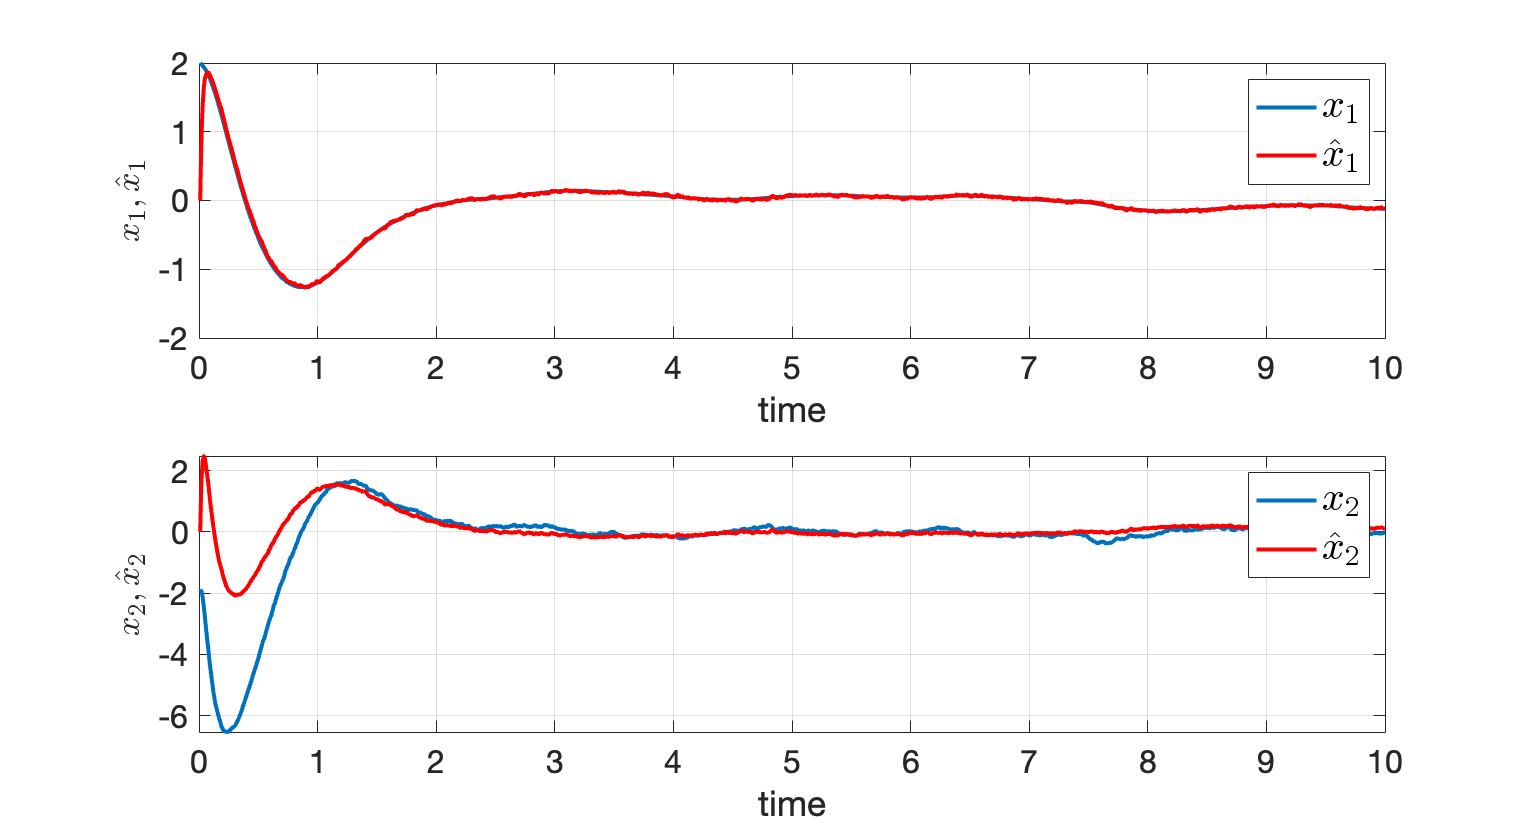
\includegraphics[width=0.8\linewidth]{images/pendulum_lqg} 

}

\caption{LQG Stabilization of Simple Pendulum.}\label{fig:pendulum-lqg}
\end{figure}

You can find code for this example \href{https://github.com/ComputationalRobotics/OptimalControlEstimation-Examples/blob/main/pendulum_stabilization_lqg.m}{here}.
\end{example}

\textbf{Closed-loop analysis}. Now that we have the Kalman filter and LQR controller implemented, let us take a look at the closed-loop response of the system. To ease our notation, let us denote \(\hat{x}_k := x^\star_{k \mid k}\) as the Kalman estimate of state. Then we can write the LQG controller as
\begin{equation}
\begin{cases}
\hat{x}_{k+1} = A \hat{x}_k + B u_k + L (y_{k+1} - C(A \hat{x}_k + B u_k) ) & \text{Kalman filter}\\
x_{k+1} = A x_k + B u_k + w_k & \text{Original dynamics}
\end{cases},
\label{eq:lqg-closed-loop-1}
\end{equation}
where \(L\) is the Kalman gain. The first equation can be simplified as
\[
\hat{x}_{k+1} = A \hat{x}_k  + Bu_k + L( C\underbrace{(A x_k + B u_k + w_k)}_{x_{k+1}} + v_{k+1} - CA\hat{x}_k - CB u_k   )\\
= A \hat{x}_k + Bu_k + L (CA x_k - CA \hat{x}_k + C w_k + v_{k+1})
\]
Let us denote the estimation error as \(e_k = x_k - \hat{x}_k\), the above equation becomes
\[
\hat{x}_{k+1} = A \hat{x}_k + B u_k + LCA e_k + LC w_k + L v_{k+1}
\]
Subtracting the equation above from the second equation of \eqref{eq:lqg-closed-loop-1}, we have
\begin{equation}
e_{k+1} = (A - LCA) e_k + (I - LC) w_k - L v_{k+1},
\label{eq:lqg-closed-loop-2}
\end{equation}
which describes the evolution of the error dynamics. Now with
\[
u_k = - K \hat{x}_k = -K (x_k - e_k) = K e_k - K x_k
\]
inserted into the second equation of \eqref{eq:lqg-closed-loop-1}, we have
\begin{equation}
x_{k+1} = (A - BK) x_k + BK e_k + w_k,
\label{eq:lqg-closed-loop-3}
\end{equation}
which describes the evolution of the true state dynamics.
Combining \eqref{eq:lqg-closed-loop-2} and \eqref{eq:lqg-closed-loop-3}, we have the closed-loop system
\begin{equation}
\begin{bmatrix} x_{k+1} \\ e_{k+1} \end{bmatrix} = \underbrace{\begin{bmatrix}
A - BK & BK \\
0 & A - LCA \end{bmatrix}}_{A_{\mathrm{cl}}} \begin{bmatrix} x_k \\ e_k \end{bmatrix} + \begin{bmatrix} w_k \\ (I - LC) w_k - L v_{k+1} \end{bmatrix}.
\label{eq:lqg-closed-loop-4}
\end{equation}
Now observe that if the Kalman gain \(L\) is stable, then \(e_{k}\) tends to zero with some noise. In this case, if the LQR gain \(K\) is stable, then the state \(x_k\) also tends to zero with some noise. In fact, since \(A_{\mathrm{cl}}\) is block-diagonal, we know the eigenvalues of \(A_{\mathrm{cl}}\) contains those of \(A - BK\) and those of \(A - LC A\).

\hypertarget{continuous-time-lqg}{%
\subsection{Continuous-time LQG}\label{continuous-time-lqg}}

\hypertarget{state-observer}{%
\section{State Observer}\label{state-observer}}

For the system \eqref{eq:output-feedback-system}, let us denote

\begin{itemize}
\item
  \(X(x_0,t_0;t;u)\) the solution at time \(t\) with input \(u\) and initial condition \(x_0\) at time \(t_0\); when \(t_0 = 0\), we write \(X(x_0;t;u)\)
\item
  \(Y(x_0,t_0;t;u)\) the output at time \(t\) with input \(u\) and initial condition \(x_0\) at time \(t_0\), i.e., \(Y(x_0,t_0;t;u) = h(X(x_0,t_0;t;u), u(t))\); when \(t_0 = 0\), we write \(y_{x_0,u}(t)\);
\item
  \(\mathcal{X}_0\) a subset of \(\mathbb{X}\) containing the initial conditions we consider; for any \(x_0 \in \mathcal{X}_0\), we write \(\sigma^+_{\mathcal{X}}(x_0;u)\) the maximal time of existence of \(X(x_0,\cdot;t;u)\) in a set \(\mathcal{X}\)
\item
  \(\mathcal{U}\) the set of all sufficiently many times differentiable inputs \(u: [0,+\infty) \rightarrow \mathbb{U}\).
\end{itemize}

The problem of state observation is to produce an estimated state \(\hat{x}(t)\) of the true state \(X(x_0,t_0;t;u)\) based on knowledge about the system \eqref{eq:output-feedback-system} and information about the history of inputs \(u_{[0,t]}\) and outputs \(y_{[0,t]}\), so that \(\hat{x}(t)\) asymptotically converges to \(X(x_0,t_0;t;u)\), for any initial condition \(x_0 \in \mathcal{X}_0\) and any input \(u \in \mathcal{U}\).

There are multiple ways for solving the problem of state observation (see e.g., \citep{bernard19book-observer}, \citep{bernard22arc-observer}). Here we are particularly interested in the approach using a \emph{state observer}, i.e., a dynamical system whose \emph{internal state} evolves according to the history of inputs and outputs, from which a state estimation can be reconstructed that guarantees asymptotic convergence to the true state. We formalize this concept below.

\begin{definition}[State Observer]
\protect\hypertarget{def:stateobserver}{}\label{def:stateobserver}A state observer for system \eqref{eq:output-feedback-system} is a couple \((\mathcal{F},\mathcal{T})\) such that

\begin{enumerate}
\def\labelenumi{\arabic{enumi}.}
\item
  \(\mathcal{F}: \mathbb{R}^{l} \times \mathbb{R}^{m} \times \mathbb{R}^d \rightarrow \mathbb{R}^l\) is continuous
\item
  \(\mathcal{T}\) is a family of continuous functions indexed by \(u \in \mathcal{U}\) where each \(\mathcal{T}_u: \mathbb{R}^l \times [0,+\infty) \rightarrow \mathbb{R}^n\) respects the causality condition
  \[
  \forall \tilde{u}: [0,+\infty) \rightarrow \mathbb{R}^m,\forall t \in [0,+\infty), u_{[0,t]} = \tilde{u}_{[0,t]} \Rightarrow  \mathcal{F}_u (\cdot,t) = \mathcal{F}_{\tilde{u}}(\cdot,t).
  \]
\item
  For any \(u \in \mathcal{U}\), any \(z_0 \in \mathbb{R}^l\), and any \(x_0 \in \mathcal{X}_0\) such that \(\sigma^+_{\mathbb{X}}(x_0;u) = +\infty\), any solution \(Z(z_0;t;u,y_{x_0,u})\)\footnote{We say ``any solution'' because there may be several solutions to the observer \eqref{eq:observer-definition-1} due to \(\mathcal{F}\) only being continuous. This is not a problem as long as any such solution satisfies the required convergence property.} to
  \begin{equation}
  \dot{z} = \mathcal{F}(z,u,y_{x_0,u})
  \label{eq:observer-definition-1}
  \end{equation}
  initialized at \(z_0\) at time \(0\) with input \(u\) and \(y_{x_0,u}\) exists on \([0,+\infty)\) and satisfies
  \begin{equation}
  \lim_{t \rightarrow \infty} \Vert \hat{X}(x_0,z_0;t;u) - X(x_0;t;u) \Vert = 0,
  \label{eq:observer-definition-2}
  \end{equation}
  with
  \begin{equation}
  \hat{X}(x_0,z_0;t;u) = \mathcal{T}_u(Z(z_0;t;u,y_{x_0,u}),t).
  \label{eq:observer-definition-3}
  \end{equation}
  In words, (i) the state observer maintains an internal state (or latent state) \(z \in \mathbb{R}^l\) that evolves according to the latent dynamics \(\mathcal{F}\) in \eqref{eq:observer-definition-1}, where \(u\) and \(y_{x_0,u}\) are inputs; (ii) an estimated state can be reconstructed from the internal state using \(\mathcal{T}_u\) as in \eqref{eq:observer-definition-3}; and (iii) the error between the estimated state and the true state (defined by a proper distance function \(\Vert \cdot \Vert\) on \(\mathbb{X}\)) converges to zero.
\end{enumerate}

If \(\mathcal{T}_u\) is the same for any \(u \in \mathcal{U}\) and is also time independent, then we say \(\mathcal{T}\) is \emph{stationary}.\footnote{The time dependence of \(\mathcal{T}_u\) enables us to cover the case where the knowledge of the \(u\) and \(y_{x_0,u}\) is used to construct the estimate from the observer state. In particular, using the output sometimes can reduce the dimension of the observer state (and thus alleviate the computations), thus obtaining a reduced-order observer. For example, see \citep{karagiannis05cdc-nonlinear} and \citep{astolfi03tac-immersion}.} In this case, we can simply write the observer \eqref{eq:observer-definition-1} and \eqref{eq:observer-definition-3} as
\begin{equation}
\begin{split}
\dot{z} &= \mathcal{F}(z,u,y) \\
\hat{x} &= \mathcal{T}(z).
\end{split}
\label{eq:observer-definition-simple}
\end{equation}

If \(\hat{x}\) can be read off directly from \(z\), then we say the observer \eqref{eq:observer-definition-simple} is \emph{in the given coordinates}. A special case of this is when \(\hat{x} = z\), i.e., the internal state of the observer is the same as the system state.
\end{definition}

\hypertarget{general-design-strategy}{%
\subsection{General Design Strategy}\label{general-design-strategy}}

\begin{theorem}[Meta Observer]
\protect\hypertarget{thm:observerdesignmeta}{}\label{thm:observerdesignmeta}Let \(F: \mathbb{R}^p \times \mathbb{R}^m \times \mathbb{R}^d \rightarrow \mathbb{R}^p\), \(H: \mathbb{R}^p \times \mathbb{R}^m \rightarrow \mathbb{R}^d\) and \(\mathcal{F}: \mathbb{R}^p \times \mathbb{R}^m \times \mathbb{R}^d \rightarrow \mathbb{R}^p\) be continuous functions such that
\begin{equation}
\dot{\hat{\xi}} = \mathcal{F}(\hat{\xi}, u, \tilde{y})
\label{eq:meta-observer-zeta-hat}
\end{equation}
is an observer for
\begin{equation}
\dot{\xi} = F(\xi,u,H(\xi,u)), \quad \tilde{y} = H(\xi,u),
\label{eq:meta-observer-zeta}
\end{equation}
i.e., for any \(\xi_0,\hat{\xi}_0 \in \mathbb{R}^p\) and any \(u \in \mathcal{U}\), the solution of the observer \eqref{eq:meta-observer-zeta-hat},
denoted by \(\hat{\Xi}(\hat{\xi}_0;t;u;\tilde{y}_{\xi_0,u})\), and the solution of the true system \eqref{eq:meta-observer-zeta}, denoted by \(\Xi(\xi_0;t;u)\), satisfy
\begin{equation}
\lim_{t \rightarrow \infty} \Vert \hat{\Xi}(\hat{\xi}_0;t;u;\tilde{y}_{\xi_0,u}) - \Xi(\xi_0;t;u) \Vert = 0.
\label{eq:meta-observer-zeta-converge}
\end{equation}
Note that the observer \eqref{eq:meta-observer-zeta-hat} is stationary and in the given coordinates for system \eqref{eq:meta-observer-zeta}. Indeed the internal state of the observer is the same as the system state.

Now suppose for any \(u \in \mathcal{U}\), there exists a continuous function (i.e., coordinate transformation) \(T_u: \mathbb{R}^n \times \mathbb{R} \rightarrow \mathbb{R}^p\) and a subset \(\mathcal{X}\) of \(\mathbb{X}\) such that

\begin{enumerate}
\def\labelenumi{\arabic{enumi}.}
\item
  For any \(x_0 \in \mathcal{X}_0\) such that \(\sigma^+_{\mathbb{X}}(x_0;u) = + \infty\), \(X(x_0;\cdot;u)\) remains in \(\mathcal{X}\)
\item
  There exists a concave \(\mathcal{K}\)\footnote{A function \(\rho: \mathbb{R}_+ \rightarrow \mathbb{R}_+\) is a \(\mathcal{K}\) function if \(\rho(0) = 0\), \(\rho\) is continuous, and \(\rho\) is increasing.} function \(\rho\) and a positive number \(\bar{t}\) such that
  \[
  \Vert x_a - x_b \Vert \leq \rho (| T_u(x_a,t) - T_u(x_b,t) |), \quad \forall x_a,x_b \in \mathcal{X}, t \geq \bar{t},
  \]
  i.e., \(x \mapsto T_u(x,t)\) becomes injective on \(\mathcal{X}\),\footnote{An injective function is a function \(f\) that maps distinct elements of its domain to distinct elements. That is, \(f(x_a) = f(x_b)\) implies \(x_a = x_b\), or equivalently, \(x_a \neq x_b\) implies \(f(x_a) \neq f(x_b)\).} uniformly in time and space, after a certain time \(\bar{t}\).
\item
  \(T_u\) transforms the system \eqref{eq:output-feedback-system} into the system \eqref{eq:meta-observer-zeta}, i.e., for all \(x \in \mathcal{X}\) and all \(t \geq 0\), we have
  \begin{equation}
  L_{(f,1)} T_u(x,t) = F(T_u(x,t),u,h(x,u)), \quad h(x,u) = H(T_u(x,t),u),
  \label{eq:meta-observer-transform}
  \end{equation}
  where \(L_{(f,1)} T_u(x,t)\) is the Lie derivative of \(T_u\) along the vector field \((f,1)\)
  \[
  L_{(f,1)} T_u(x,t) = \lim_{\tau \rightarrow 0} \frac{ T_u (X(x,t;t+\tau;u),t+\tau) - T_u(x,t) }{\tau}.
  \]
\item
  \(T_u\) respects the causality condition
  \[
  \forall \tilde{u}: [0,+\infty) \rightarrow \mathbb{R}^m, \forall t \in [0,+\infty), u_{[0,t]} = \tilde{u}_{[0,t]} \Rightarrow T_u(\cdot,t) = T_{\tilde{u}}(\cdot,t).
  \]
\end{enumerate}

Then, for any \(u \in \mathcal{U}\), there exists a function \(\mathcal{T}_u: \mathbb{R}^p \times [0,+\infty) \rightarrow \mathcal{X}\) (satisfying the causality condition) such that for any \(t \geq \bar{t}\), \(\xi \mapsto \mathcal{T}_u (\xi, t)\) is uniformly continuous on \(\mathbb{R}^p\) and satisfies
\[
\mathcal{T}_u \left( T_u(x,t),t \right) = x, \forall x \in \mathcal{X}.
\]
Moreover, denoting \(\mathcal{T}\) the family of functions \(\mathcal{T}_u\) for \(u \in \mathcal{U}\), the couple \((\mathcal{F}, \mathcal{T})\) is an observer for the system \eqref{eq:output-feedback-system} initialized in \(\mathcal{X}_0\).
\end{theorem}

\begin{proof}
See Theorem 1.1 in \citep{bernard19book-observer}.
\end{proof}

A simpler version of Theorem \ref{thm:observerdesignmeta} where the coordinate transformation \(T_u\) is stationary and fixed for all \(u\) is stated below as a corollary.

\begin{corollary}[Meta Observer with Fixed Transformation]
\protect\hypertarget{cor:observerdesignmetafixedT}{}\label{cor:observerdesignmetafixedT}Let \(F: \mathbb{R}^p \times \mathbb{R}^m \times \mathbb{R}^d \rightarrow \mathbb{R}^p\), \(H: \mathbb{R}^p \times \mathbb{R}^m \rightarrow \mathbb{R}^d\) and \(\mathcal{F}: \mathbb{R}^p \times \mathbb{R}^m \times \mathbb{R}^d \rightarrow \mathbb{R}^p\) be continuous functions such that \eqref{eq:meta-observer-zeta-hat} is an observer for \eqref{eq:meta-observer-zeta}.

Suppose there exists a continuous coordinate transformation \(T: \mathbb{R}^p \rightarrow \mathbb{R}^n\) and a compact subset \(\Omega\) of \(\mathbb{R}^n\) such that

\begin{enumerate}
\def\labelenumi{\arabic{enumi}.}
\item
  For any \(x_0 \in \mathcal{X}_0\) such that \(\sigma^+_{\mathbb{X}}(x_0;u) = + \infty\), \(X(x_0;\cdot;u)\) remains in \(\Omega\)
\item
  \(x \mapsto T(x)\) is injective on \(\Omega\)
\item
  \(T\) transforms the system \eqref{eq:output-feedback-system} into system \eqref{eq:meta-observer-zeta}
  \[
  L_f T(x) = F(T(x),u,h(x,u)), \quad h(x,u) = H(T(x),u),
  \]
  where \(L_f T(x)\) is the Lie derivative of \(T(x)\) along \(f\)
  \[
  L_f T(x) = \lim_{\tau \rightarrow 0} \frac{ T(X(x,t;t+\tau;u))  - T(x)}{\tau}.
  \]
\end{enumerate}

Then, there exists a uniformly continuous function \(\mathcal{T}:\mathbb{R}^p \rightarrow \mathbb{R}^{n}\) such that
\[
\mathcal{T}(T(x)) = x, \quad \forall x \in \Omega,
\]
and \((\mathcal{F},\mathcal{T})\) is an observer for system \eqref{eq:output-feedback-system} initialized in \(\mathcal{X}_0\).
\end{corollary}

Theorem \ref{thm:observerdesignmeta} and Corollary \ref{cor:observerdesignmetafixedT} suggest the following general observer design strategy:

\begin{enumerate}
\def\labelenumi{\arabic{enumi}.}
\item
  Find an injective coordinate transformation \(T_u\) (that may be time-varying and also dependent on \(u\)) that transforms the original system \eqref{eq:output-feedback-system} with coordinate \(x\) into a new system \eqref{eq:meta-observer-zeta} with coordinate \(\xi\)
\item
  Design an observer \eqref{eq:meta-observer-zeta-hat}, \(\hat{\xi}\), for the new system
\item
  Compute a left inverse, \(\mathcal{T}_u\), of the transformation \(T_u\) to recover a state estimation \(\hat{x}\) of the original system.
\end{enumerate}

The transformed systems \eqref{eq:meta-observer-zeta} are typically referred to as \emph{normal forms}, or in my opinion, \emph{templates}.

Of course, the general design strategy is rather conceptual, and in order for it to be practical, we have to answer three questions.

\begin{itemize}
\item
  What templates do we have, what are their associated observers, and what are the conditions for the observers to be asymptotically converging?
\item
  What kinds of (nonlinear) systems can be transformed into the templates, and how to perform the transformation?
\item
  How to invert the coordinate transformation? Is it analytical or does it require numerical approximation?
\end{itemize}

In the following sections, we will study several representative normal forms and answer the above questions. Before presenting the results, let us first introduce several notions of observability.

\begin{definition}[Observability]
\protect\hypertarget{def:observability}{}\label{def:observability}

Consider an open subset \(\mathcal{L}\) of the state space \(\mathbb{X} \subseteq \mathbb{R}^n\) of system \eqref{eq:output-feedback-system}. The system \eqref{eq:output-feedback-system} is said to be

\begin{itemize}
\item
  \textbf{Distinguishable} on \(\mathcal{L}\) for some input \(u(t)\), if for all \((x_a,x_b) \in \mathcal{L} \times \mathcal{L}\),
  \[
  y_{x_a,u}(t) = y_{x_b,u}(t), \forall t \in [0,\min\left\{\sigma^+_{\mathbb{X}}(x_a;u), \sigma^+_{\mathbb{X}}(x_b;u) \right\}] \Longrightarrow x_a = x_b
  \]
\item
  \textbf{Instantaneously distinguishable} on \(\mathcal{L}\) for some input \(u(t)\), if for all \((x_a,x_b) \in \mathcal{L} \times \mathcal{L}\), and for all \(\bar{t} \in (0, \min\left\{\sigma^+_{\mathbb{X}}(x_a;u), \sigma^+_{\mathbb{X}}(x_b;u) \right\})\),
  \[
  y_{x_a,u}(t) = y_{x_b,u}(t), \forall t \in [0,\bar{t}) \Longrightarrow x_a = x_b
  \]
\item
  \textbf{Uniformly observable} on \(\mathcal{L}\) if it is distinguishable on \(\mathcal{L}\) for any input \(u(t)\) (not only for \(u \in \mathcal{U}\))
\item
  \textbf{Uniformly instantaneously observable} on \(\mathcal{L}\) if it is instantaneously observable on \(\mathcal{L}\) for any input \(u(t)\) (not only for \(u \in \mathcal{U}\)).
\end{itemize}

Moreover, let \(\mathcal{X}\) be a subset of \(\mathbb{X}\) such that \(\mathrm{cl}(\mathcal{X})\), i.e., the closure of \(\mathcal{X}\), is contained in \(\mathcal{L}\). Then the system \eqref{eq:output-feedback-system} is said to be

\begin{itemize}
\tightlist
\item
  \textbf{Backward \(\mathcal{L}\)-distinguishable on \(\mathcal{X}\)} for some input \(u(t)\), if for any \((x_a,x_b) \in \mathcal{X} \times \mathcal{X}\) such that \(x_a \neq x_b\), there exists \(t \in (\max\left\{ \sigma^{-}_{\mathcal{L}}(x_a;u), \sigma^{-}_{\mathcal{L}}(x_b;u) \right\},0]\) such that \(y_{x_a,u}(t) \neq y_{x_b,u}(t)\), or in words similar to the definition of distinguishable on \(\mathcal{L}\), for all \((x_a,x_b) \in \mathcal{X} \times \mathcal{X}\)
  \[
  y_{x_a,u}(t) = y_{x_b,u}(t), \forall t \in (\max\left\{\sigma^{-}_{\mathcal{L}}(x_a;u), \sigma^{-}_{\mathcal{L}}(x_b;u) \right\},0] \Longrightarrow x_a = x_b.
  \]
\end{itemize}

\end{definition}

\hypertarget{luenberger-template}{%
\subsection{Luenberger Template}\label{luenberger-template}}

Consider an instance of the normal form \eqref{eq:meta-observer-zeta} as follows:
\begin{equation}
\dot{\xi} = A \xi + B(u,y), \quad y = C \xi,
\label{eq:Luenberger-linear-template}
\end{equation}
where \(A,C\) are constant matrices, and \(B(u,y)\) can depend nonlinearly on \(u\) and \(y\).

For this template, we have the well-known Luenberger observer.

\begin{theorem}[Luenberger Observer]
\protect\hypertarget{thm:LuenbergerLinear}{}\label{thm:LuenbergerLinear}If the pair \((A,C)\) is detectable (see Theorem \ref{thm:ltidetectable}), then there exists a matrix \(K\) such that \(A-KC\) is Hurwitz and the system
\begin{equation}
\dot{\hat{\xi}} = A \hat{\xi} + B(u,y) + K(y - C \hat{\xi})
\label{eq:Luenberger-Linear}
\end{equation}
is an observer for \eqref{eq:Luenberger-linear-template}.
\end{theorem}

\begin{proof}
Define \(e(t) = \xi(t) - \hat{\xi}(t)\). In that case,
\begin{equation}
    \dot{e}(t) = [A - KC] e(t)
    \label{eq:Luenberger-error}
\end{equation}

Solving \eqref{eq:Luenberger-error}, we obtain

\begin{equation}
    e(t) = \mathrm{exp}[(A - KC)t] e(0)
\end{equation}

Then, if the real components of the eigenvalues of \(A - KC\) are strictly negative (i.e., \(A - KC\) is Hurwitz), then \(e(t) \rightarrow 0\) as \(t \rightarrow \infty\), independent of the initial error \(e(0) = \xi(0) - \hat{\xi}(0)\). From Theorem \ref{thm:ltidetectable}, we know that \((A,C)\) being detectable implies the existence of \(K\) such that \(A - KC\) is Hurwitz.

If one is further interested in estimating the convergence rate of the Luenberger observer, then one can use the result from Corollary \ref{cor:bestconvergencerate}. Particularly, one can solve the Lyapunov equation
\[
(A - KC)^T P + P (A - KC) = - I
\]
to obtain \(P\). Then the convergence rate of \(\Vert e \Vert\) towards zero is \(\frac{0.5}{\lambda_{\max}(P)}\).
\end{proof}

The Luenberger observer is an elegant result in observer design (and even in control theory) that has far-reaching impact. In my opinion, the essence of observer design is twofold: (i) to simulate the dynamics when the state estimation is correct, and (ii) to correct the state estimation from observation when it is off. These two pieces of ideas are evident in \eqref{eq:Luenberger-Linear}: the observer is a copy of the original dynamics (\(A \hat{\xi} + B(u,y)\)) plus a feedback correction from the difference between the ``imagined'' observation \(C\hat{\xi}\) and the true observation \(y\).

You may think the Luenberger template is restricting because it requires the system to be linear (up to the only nonlinearly in \(B(u,y)\)). However, it turns out the Luenberger template is already quite useful, as I will show in the following pendulum example.

\begin{example}[Luenberger Observer for A Simple Pendulum]
\protect\hypertarget{exm:pendulumLuenberger}{}\label{exm:pendulumLuenberger}Consider a simple pendulum dynamics model
\begin{equation}
x = \begin{bmatrix}
\theta \\ \dot{\theta}
\end{bmatrix}, \quad 
\dot{x} = \begin{bmatrix} 
\dot{\theta} \\
- \frac{1}{ml^2} (b \dot{\theta} + mgl \sin \theta) 
\end{bmatrix} + 
\begin{bmatrix}
0 \\
\frac{1}{ml^2} 
\end{bmatrix} u, \quad y = \theta,
\label{eq:kbobserver-pendulum}
\end{equation}
where \(\theta\) the angular position of the pendulum from the vertical line, \(m > 0\) the mass of the pendulum, \(l > 0\) the length, \(g\) the gravitational constant, \(b > 0\) the dampling coefficient, and \(u\) the control input (torque).

We assume we can only observe the angular position of the pendulum in \eqref{eq:kbobserver-pendulum}, e.g., using a camera, but not the angular velocity. Our goal is to construct an observer that can provide a full state estimation.

We first note that the pendulum dynamics \eqref{eq:kbobserver-pendulum} can actually be written in the (linear) Luenberger template \eqref{eq:Luenberger-linear-template} as\footnote{I have to say I was a bit surprised when I arrived at this formulation.}
\begin{equation}
\begin{split}
\dot{x} & = \underbrace{\begin{bmatrix}
0 & 1 \\
0 & - \frac{b}{ml^2}
\end{bmatrix}}_{=:A} x + 
\underbrace{\begin{bmatrix}
0 \\
\frac{u - mgl \sin \theta }{ml^2}
\end{bmatrix}}_{=:B(u,y)} \\
y & = \underbrace{\begin{bmatrix}
1 & 0
\end{bmatrix}}_{=:C} x 
\end{split}.
\label{eq:pendulum-Luenberger-Linear}
\end{equation}

In order for us to use the Luenberger observer, we need to check if the pair \((A,C)\) is detectable. We can easily find the eigenvalues and eigenvectors of \(A\):
\[
A \begin{bmatrix}
1 \\ 0
\end{bmatrix} = 0,\quad 
A \begin{bmatrix}
- \frac{ml^2}{b} \\ 1 
\end{bmatrix} = \begin{bmatrix}
1 \\ - \frac{b}{ml^2}
\end{bmatrix}
= - \frac{b}{ml^2} \begin{bmatrix}
- \frac{ml^2}{b} \\ 1 \end{bmatrix}.
\]
The first eigenvalue has real part equal to \(0\). However,
\[
C \begin{bmatrix}
1 \\ 0
\end{bmatrix} = 1 \neq 0.
\]
According to Theorem \ref{thm:ltidetectable}, we conclude \((A,C)\) is detectable. In fact, the pair \((A,C)\) is more than just detectable, it is indeed observable (according to Theorem \ref{thm:ltiobservable}). Therefore, the poles of \(A - KC\) can be arbitrarily placed.

\textbf{Finding \(K\)}. Now we need to find \(K\). An easy choice of \(K\) is
\[
K = \begin{bmatrix} k \\ 0 \end{bmatrix}, \quad A - KC = 
\begin{bmatrix}
- k & 1 \\ 0 & - \frac{b}{ml^2}
\end{bmatrix}.
\]
With \(k > 0\), we know \(A- KC\) is guaranteed to be Hurwitz (the two eigenvalues of \(A-KC\) are \(-k\) and \(-b/ml^2\)), and we have obtained an observer!

We can also estimate the convergence rate of this observer. Let us use \(m=1,g=9.8,l=1,b=0.1\) as parameters of the pendulm dynamics. According to Theorem \ref{thm:LuenbergerLinear}, we solve the Lyapunov equation
\[
(A - KC)^T P + P(A - KC) = -I
\]
and \(\gamma = \frac{0.5}{\lambda_{\max}(P)}\) will be our best estimate of the convergence rate (of \(\Vert e \Vert = \Vert \hat{x} - x \Vert\) towards zero).

Table \ref{tab:pendulumLuenbergerRate} below shows the convergence rates computed for different values of \(k\). We can see that as \(k\) is increased, the convergence rate estimation is also increased. However, it appears that \(0.1\) is the best convergence rate we can achieve, regardless of how large \(k\) is.

\begin{longtable}[]{@{}
  >{\centering\arraybackslash}p{(\columnwidth - 12\tabcolsep) * \real{0.1512}}
  >{\centering\arraybackslash}p{(\columnwidth - 12\tabcolsep) * \real{0.1395}}
  >{\centering\arraybackslash}p{(\columnwidth - 12\tabcolsep) * \real{0.1512}}
  >{\centering\arraybackslash}p{(\columnwidth - 12\tabcolsep) * \real{0.1395}}
  >{\centering\arraybackslash}p{(\columnwidth - 12\tabcolsep) * \real{0.1395}}
  >{\centering\arraybackslash}p{(\columnwidth - 12\tabcolsep) * \real{0.1395}}
  >{\centering\arraybackslash}p{(\columnwidth - 12\tabcolsep) * \real{0.1395}}@{}}
\caption{\label{tab:pendulumLuenbergerRate} Convergence rate estimation of the Luenberger observer for a simple pendulm.}\tabularnewline
\toprule()
\begin{minipage}[b]{\linewidth}\centering
\(k\)
\end{minipage} & \begin{minipage}[b]{\linewidth}\centering
\(0.1\)
\end{minipage} & \begin{minipage}[b]{\linewidth}\centering
\(1\)
\end{minipage} & \begin{minipage}[b]{\linewidth}\centering
\(10\)
\end{minipage} & \begin{minipage}[b]{\linewidth}\centering
\(100\)
\end{minipage} & \begin{minipage}[b]{\linewidth}\centering
\(1000\)
\end{minipage} & \begin{minipage}[b]{\linewidth}\centering
\(10000\)
\end{minipage} \\
\midrule()
\endfirsthead
\toprule()
\begin{minipage}[b]{\linewidth}\centering
\(k\)
\end{minipage} & \begin{minipage}[b]{\linewidth}\centering
\(0.1\)
\end{minipage} & \begin{minipage}[b]{\linewidth}\centering
\(1\)
\end{minipage} & \begin{minipage}[b]{\linewidth}\centering
\(10\)
\end{minipage} & \begin{minipage}[b]{\linewidth}\centering
\(100\)
\end{minipage} & \begin{minipage}[b]{\linewidth}\centering
\(1000\)
\end{minipage} & \begin{minipage}[b]{\linewidth}\centering
\(10000\)
\end{minipage} \\
\midrule()
\endhead
\(\gamma\) & \(0.0019\) & \(0.0523\) & \(0.0990\) & \(0.1000\) & \(0.1000\) & \(0.1000\) \\
\bottomrule()
\end{longtable}

\textbf{Optimal \(K\)}. Is it true that \(0.1\) is the best convergence rate, or in other words, what is the best \(K\) that maximizes the convergence rate \(\gamma\)?

A natural way (and my favorite way) to answer this question is to formulate an optimization problem.
\begin{equation}
\begin{split}
\min_{P,K} & \quad \lambda_{\max}(P) \\
\text{subject to} & \quad (A - KC)^T P + P (A - KC) = -I \\
& \quad P \succeq 0
\end{split}
\label{eq:pendulumLuenbergerMaxgammaNonCVX}
\end{equation}
The above formulation seeks the best possible \(K\) that minimizes \(\lambda_{\max}(P)\) which, according to \(\gamma = 0.5 / \lambda_{\max}(P)\), also maximizes \(\gamma\).

However, problem \eqref{eq:pendulumLuenbergerMaxgammaNonCVX} is not a convex formulation due to the bilinear term \(PK\). Nevertheless, via a simple change of variable \(H = PK\), we arrive at the following convex formulation
\begin{equation}
\begin{split}
\min_{P,H} & \quad \lambda_{\max}(P) \\
\text{subject to} & \quad A^T P - C^T H^T + PA - H C = - I \\
& \quad P \succeq 0
\end{split}
\label{eq:pendulumLuenbergerMaxgammaCVX}
\end{equation}
Problem \eqref{eq:pendulumLuenbergerMaxgammaCVX} is a semidefinite programming problem (SDP), that can be modeled and solved by off-the-shelf tools. We can recover \(K = P^{-1} H\) from \eqref{eq:pendulumLuenbergerMaxgammaCVX} after it is solved.

Interestingly, solving problem \eqref{eq:pendulumLuenbergerMaxgammaCVX} verifies that the minimum \(\lambda_{\max}(P)\) is \(5\) and the maximum converge rate is \(0.1\). An optimal solution of \eqref{eq:pendulumLuenbergerMaxgammaCVX} is
\[
P^\star = \begin{bmatrix}
2.4923 & 0 \\ 0 & 5 \end{bmatrix}, \quad 
K^\star = \begin{bmatrix}
0.2006 \\ 0.4985 \end{bmatrix}.
\]
You should check out the Matlab code of this example \href{https://github.com/ComputationalRobotics/OptimalControlEstimation-Examples/blob/main/pendulum_luenberger.m}{here}.
\end{example}

\hypertarget{state-affine-template}{%
\subsection{State-affine Template}\label{state-affine-template}}

Consider an instance of the normal form \eqref{eq:meta-observer-zeta} where the dynamics is linear in \(\xi\), but the coefficients are time-varying and dependent on the input and output
\begin{equation}
\dot{\xi} = A(u,y) \xi + B(u,y), \quad y = C(u) \xi.
\label{eq:state-affine-template}
\end{equation}
The difference between the state-affine template \eqref{eq:state-affine-template} and the Luenberger template \eqref{eq:Luenberger-linear-template} is that the linear matrices \(A,C\) are allowed to depend nonlinearly on the input \((u,y)\).

Kalman and Bucy originally proposed an observer for linear time-varying systems \citep{kalman61-new}. The result is later extened by \citep{besanccon96ejc-observer} and \citep{hammouri90cdc-observer} to deal with coefficient matrices dependent on the control. The following theorem is a direct extension of the result from \citep{besanccon96ejc-observer} and \citep{hammouri90cdc-observer} by considering \((u,y)\) as an augmented control input.

Before presenting the theorem, we need to introduce the following terminology.

\begin{definition}[Linear Time-Varying System]
\protect\hypertarget{def:lineartimevarying}{}\label{def:lineartimevarying}

For a linear time-varying system of the form
\begin{equation}
\dot{\chi} = A(\nu) \chi, \quad y = C(\nu) \chi,
\label{eq:linear-time-varying}
\end{equation}
with input \(\nu\) and output \(y\), we define

\begin{itemize}
\item
  the \emph{transition matrix} \(\Psi_\nu\) as the unique solution to
  \[
  \Psi_\nu (t,t) = I, \quad \frac{\partial \Psi_\nu}{\partial \tau}(\tau,t) = A(\nu(\tau)) \Psi_\nu (\tau, t).
  \]
  Note that the transition matrix is used to express the solution to \eqref{eq:linear-time-varying} because it satisfies
  \[
  \chi(\chi_0,t_0;t;\nu) = \Psi_\nu (t,t_0) \chi_0.
  \]
\item
  the \emph{observability grammian} as
  \[
  \Gamma_\nu (t_0,t_1) = \int_{t_0}^{t_1} \Psi_\nu (\tau,t_0)^T C(\nu(\tau))^T C(\nu(\tau)) \Psi_\nu (\tau,t_0) d\tau.
  \]
\item
  the \emph{backward observability grammian} as
  \[
  \Gamma_\nu^b (t_0,t_1) = \int_{t_0}^{t_1} \Psi_\nu (\tau,t_1)^T C(\nu(\tau))^T C(\nu(\tau)) \Psi_\nu (\tau,t_1) d\tau.
  \]
\end{itemize}

\end{definition}

We now introduce the Kalman-Bucy Observer for the state-affine template \eqref{eq:state-affine-template}.

\begin{theorem}[Kalman-Bucy Observer]
\protect\hypertarget{thm:kalmanbucystateaffine}{}\label{thm:kalmanbucystateaffine}Let \(y_{\xi_0,u}(t) = C(u(t)) \Xi (\xi_0;t;u)\) be the output of system \eqref{eq:state-affine-template} at time \(t\) with initialization \(\xi_0\) and control \(u\). Suppose the control \(u\) satisfies

\begin{itemize}
\item
  For any \(\xi_0\), \(t \mapsto A(u(t),y_{\xi_0,u}(t))\) is bounded by \(A_{\max}\)
\item
  For any \(\xi_0\), the augmented input \(\nu = (u,y_{\xi_0,u})\) is \emph{regularly persistent} for the dynamics
  \begin{equation}
  \dot{\chi} = A(\nu) \chi , \quad y = C(\nu) \chi 
  \label{eq:kbobserver-auxilarydynamics}
  \end{equation}
  uniformly with respect to \(\xi_0\). That is, there exist strictly positive numbers \(t_0,\bar{t}\), and \(\alpha\) such that for any \(\xi_0\) and any time \(t \geq t_0 \geq \bar{t}\),
  \[
  \Gamma_v^b (t-\bar{t}, t) \succeq \alpha I,
  \]
  where \(\Gamma_v^b\) is the \emph{backward observability grammian} associated with system \eqref{eq:kbobserver-auxilarydynamics}.
\end{itemize}

Then, given any positive definite matrix \(P_0\), there exist \(\alpha_1,\alpha_2 > 0\) such that for any \(\lambda \geq 2 A_{\max}\) and any \(\xi_0 \in \mathbb{R}^p\), the matrix differential equation
\begin{equation}
\dot{P} = -\lambda P - A(u,y)^T P - P A(u,y) + C(u)^T C(u)
\label{eq:kbobserver-matrixdifferential}
\end{equation}
initialized at \(P(0) = P_0\) admits a unique solution satisfying \(P(t)=P(t)^T\) and
\[
\alpha_2 I \succeq P(t) \succeq \alpha_1 I.
\]
Moreover, the system
\begin{equation}
\dot{\hat{\xi}} = A(u,y) \hat{\xi} + B(u,y) + K (y - C(u)\hat{\xi})
\label{eq:kbobserver-observer}
\end{equation}
with a time-varying gain matrix
\begin{equation}
K = P^{-1} C(u)^T 
\label{eq:kbobserver-gain}
\end{equation}
is an observer for the state-affine system \eqref{eq:state-affine-template}.
\end{theorem}

Let us work out an example of the Kalman-Bucy Observer for nonlinear systems.

\begin{example}[Kalman-Bucy Observer for A Simple Pendulum]
\protect\hypertarget{exm:pendulumkbobserver}{}\label{exm:pendulumkbobserver}

Let us reconsider the pendulum dynamics \eqref{eq:kbobserver-pendulum} but this time try to design a Kalman-Bucy observer.

We first write the pendulum dynamics in a new coordinate system so that it is in the state-affine normal form \eqref{eq:state-affine-template}. We choose \(\xi = [\mathfrak{s},\mathfrak{c},\dot{\theta}]^T\) with \(\mathfrak{s} = \sin \theta\) and \(\mathfrak{c} = \cos \theta\). Clearly, we will be able to observe \(y = [\mathfrak{s},\mathfrak{c}]^T\) in this new coordinate. The state-affine normal form of the pendulum dynamics reads
\begin{equation}
\begin{split}
\dot{\xi} = \begin{bmatrix}
\mathfrak{c} \dot{\theta} \\
- \mathfrak{s} \dot{\theta} \\
- \frac{1}{ml^2} (b \dot{\theta} + mgl \mathfrak{s} ) +  \frac{1}{ml^2} u
\end{bmatrix} & = 
\underbrace{\begin{bmatrix}
0 & 0 & \mathfrak{c} \\
0 & 0 & -\mathfrak{s} \\
0 & 0 & -\frac{b}{ml^2}
\end{bmatrix}}_{=:A(u,y)} \xi + 
\underbrace{\begin{bmatrix}
0 \\ 0 \\ \frac{u - mgl \mathfrak{s}}{ml^2}
\end{bmatrix}}_{=:B(u,y)} \\
y & = \underbrace{\begin{bmatrix}
1 & 0 & 0 \\
0 & 1 & 0
\end{bmatrix}}_{=:C(u)} \xi
\end{split}.
\label{eq:pendulum-state-affine}
\end{equation}
Note that \(C(u)\) is in fact time-invariant, and \(B(u,y)\) only depends on \(u\); but we adopt the same notation as the general state-affine template \eqref{eq:state-affine-template}.

In order to use the Kalman-Bucy observer in Theorem \ref{thm:kalmanbucystateaffine}, we need to verify the boundedness of \(A(u,y)\), and the regular persistence of \eqref{eq:kbobserver-auxilarydynamics}.

\textbf{Boundedness of \(A(u,y)\)}. We can easily show the boundedness of \(A(u,y)\) by writing
\[
\Vert A(u,y) \xi \Vert = \Vert \xi_3 (\mathfrak{c} - \mathfrak{s} - b/ml^2) \Vert  \leq |\xi_3| \sqrt{3} \sqrt{\mathfrak{c}^2 + \mathfrak{s}^2 + b^2 / m^2 l^4} \leq \Vert \xi \Vert \sqrt{3 + 3b^2 / m^2 l^4}. 
\]
Therefore, we can take \(A_{\max} = \sqrt{3 + 3b^2 / m^2 l^4}\).

\textbf{Regular persistence}. We write the backward observability grammian of system \eqref{eq:kbobserver-auxilarydynamics}
\[
\Gamma_\nu^b(t - \bar{t},t) = \int_{t - \bar{t}}^t \Psi_\nu(\tau,t)^T C^T C \Psi_\nu (\tau, t) d \tau = \int_{t - \bar{t}}^t \Psi_\nu(\tau,t)^T \underbrace{\begin{bmatrix} 
1 & 0 & 0 \\
0 & 1 & 0 \\
0 & 0 & 0
\end{bmatrix}}_{=:\tilde{C}}
\Psi_\nu (\tau, t) d \tau.
\]
\(\Gamma_\nu^b(t - \bar{t},t) \succeq \alpha I\) if and only if
\[
w^T \Gamma_\nu^b(t - \bar{t},t) w \geq \alpha, \quad \forall w \in \mathbb{R}^3, \Vert w \Vert = 1.
\]
With this, we develop \(w^T \Gamma_\nu^b(t - \bar{t},t) w\)
\begin{equation}
\begin{split}
w^T \Gamma_\nu^b(t - \bar{t},t) w &= \int_{t - \bar{t}}^t s^T \tilde{C} s d\tau, \\
& = \int_{t - \bar{t}}^t \left( s_1^2 + s_2^2 \right) d\tau, \quad s = \Psi_\nu (\tau, t) w
\end{split}
\label{eq:pendulm-regular-persistence-1}
\end{equation}
and observe that \(s = \Psi_\nu (\tau,t) w\) is equivalent to
\[
w = (\Psi_\nu (\tau,t))^{-1} s = \Psi_\nu (t,\tau) s,
\]
that is, \(w\) is the solution of \(\dot{\xi} = A(\nu) \xi\) at time \(t\) with initial condition \(s\) at time \(\tau \leq t\). Equivalently, this is saying \(s\) is the initial condition of \(\dot{\xi} = A(\nu) \xi\) at time \(\tau \leq t\) such that its solution at time \(t\) is \(w\). Note that from \eqref{eq:pendulm-regular-persistence-1} it is clearly that \(\int_{t - \bar{t}}^t \left( s_1^2 + s_2^2 \right) d\tau \geq 0\), and \(\int_{t - \bar{t}}^t \left( s_1^2 + s_2^2 \right) d\tau = 0\) if and only if \(s_1^2 + s_2^2 = 0\), or equivalently \(s_1 = s_2 = 0\) for any \(\tau \in [t - \bar{t}, t]\).

We then take a closer look at the system \(\dot{\xi} = A(\nu) \xi\):
\begin{equation}
\begin{split}
\dot{\xi}_1 &= \mathfrak{c} \xi_3 \\
\dot{\xi}_2 &= -\mathfrak{s} \xi_3 \\
\dot{\xi}_3 &= - \frac{b}{ml^2} \xi_3.
\end{split}
\label{eq:pendulm-state-affine-auxiliarysystem}
\end{equation}

If the solution of \(\xi_3\) at time \(t\) is \(w_3\), then
\[
\xi_3(\tau) = w_3 e^{\frac{b}{ml^2}(t - \tau)}, \quad \tau \leq t.
\]
We can now claim it is impossible that \(s_1 = s_2 = 0\) at any time \(\tau \in [t - \bar{t}, t]\).

We can show this by contradiction. First of all, \(s_1 = s_2 = 0\) at \(\tau = t\) implies \(w_1 = w_2 = 0\) and hence \(w_3 = \pm 1\). This implies \(\xi_3 \neq 0\) for any \(\tau \in [t - \bar{t}, t]\). Then, \(s_1 = 0, \forall \tau \in [t - \bar{t}, t]\) implies \(\dot{\xi}_1 = 0\) which, due to \(\xi_3 \neq 0\), implies \(\mathfrak{c} = 0\) for all \(\tau\). Similarly, \(s_2 = 0, \forall \tau \in [t - \bar{t}, t]\) implies \(\dot{\xi}_2 = 0\) and \(\mathfrak{s} = 0\). This creates a contradiction because \(\mathfrak{c}^2 + \mathfrak{s}^2 = 1\) and \(\mathfrak{c}, \mathfrak{s}\) cannot be simultaneously zero.

The above reasoning proves that the backward observability Grammian is positive definite, which is, however, still insufficient for the Kalman-Bucy observer. We need a stronger uniformly positive definite condition on \(\Gamma_\nu^b\), i.e., to find \(t_0, \bar{t}\) and \(\alpha>0\) so that \(\Gamma_\nu^b(t-\bar{t},t) \succeq \alpha I\) for all \(t \geq t_0\).

If the control \(u\) is unbounded, then sadly, one can show that the uniform positive definite condition fails to hold, as left by you to show in the following exercise.

\begin{exercise}[Counterexample for Kalman-Bucy Observer]
\protect\hypertarget{exr:kbobserverpendulumcounterexample}{}\label{exr:kbobserverpendulumcounterexample}Show that, if the control \(u\) is unbounded, then for any \(\alpha > 0\), \(t_0 \geq \bar{t} > 0\), there exists \(t \geq t_0\) such that \(\Gamma_\nu^b(t - \bar{t},t) \prec \alpha I\). (Hint: consider a controller that spins the pendulum faster and faster such that in time \(\bar{t}\) it has rotated \(2k\pi\), in this case the angular velocity becomes unobservable because we are not sure how many rounds the pendulum has rotated.)
\end{exercise}

Fortunately, if the control \(u\) is bounded, then we can prove the uniform positive define condition holds for \(\Gamma_\nu^b(t - \bar{t},t)\). The following proof is given by \href{https://scholar.harvard.edu/weiyuli/home}{Weiyu Li}.

Without loss of generality, let \(\frac{b}{ml^2} = 1\). Assume \(u\) is bounded such that the third entry of \(B(u,y)\) in \eqref{eq:pendulum-state-affine} is bounded by \(\beta > 0\)
\[
\left| \frac{u - mgl \mathfrak{s}}{ml^2} \right| \leq \beta.
\]
Assuming the initial velocity of the pendulum is \(\dot{\theta}(0) = \dot{\theta}_0\), we know \(\dot{\theta}(t)\) is bounded by
\[
\dot{\theta}(t) \in \left[ c_1(1-\beta)e^{-t} - \beta  , c_2(1-\beta)e^{-t} + \beta \right],
\]
where \(c_1,c_2\) are constants chosen to satisfy the initial condition. Clearly, for all \(t > 0\), we see \(\dot{\theta}(t)\) is bounded, and hence we know \(\dot{\mathfrak{c}}\) and \(\dot{\mathfrak{s}}\) are bounded (due to \(\mathfrak{c}\) and \(\mathfrak{s}\) are bounded). Intuitively, what we have just shown says that when the control is bounded, the measurements \(\mathfrak{c}\) and \(\mathfrak{s}\) will have bounded time derivatives. (This will help us analyze the auxiliary system \eqref{eq:pendulm-state-affine-auxiliarysystem}.)

Now back to checking regular persistence of the auxilary system \eqref{eq:pendulm-state-affine-auxiliarysystem}. We will discuss two cases: (1) \(w_3^2 > 1 - \delta\), and (2) \(w_3^2 \leq 1 - \delta\), for some constant \(\delta < 0.5\) determined later.

\begin{enumerate}
\def\labelenumi{\arabic{enumi}.}
\item
  \(w_3^2 > 1 - \delta > 0.5\). In this case we have \(w_1^2 + w_2^2 = 1 - w_3^2 < \delta\), and hence \(w_1^2 < \delta\), \(w_2^2 < \delta\). On the other hand, from \eqref{eq:pendulm-state-affine-auxiliarysystem} we have
  \[
  \dot{\xi}_1^2(\tau) + \dot{\xi}_2^2(\tau) = \xi_3^2 = w_3^2 e^{2 (t - \tau)} > w_3^2 > 1 - \delta, \quad \forall \tau < t.
  \]
  Without loss of generality assume \(\dot{\xi}_1(t)^2 > (1-\delta)/2\). As \(\dot{\xi}_1 = \mathfrak{c} \xi_3\) and both \(\mathfrak{c}\) and \(\xi_3\) have bounded derivatives, we know \(\dot{\xi}_1\) will not change sign for some duration \(T\) that is independent from the choice of \(\delta\) (because the time derivatives of \(\mathfrak{c}\) and \(\xi_3\) do not depend on \(\delta\)). That is \(|\dot{\xi}_1| > \sqrt{(1-\delta)/2} > 1/2\) for \(\tau \in [t - T,t]\). Consequently,
  \[
  |\xi_1(t - \tau)| > \frac{1}{2} \tau - |w_1| > \frac{1}{2} \tau - \sqrt{\delta}, \quad \tau \in [0,T].
  \]
  Choosing \(\delta\) small enough, we have \(|\xi_1(t - \tau)| > 0.25 \tau\) for \(\tau \in [0.5T,T]\). Then we have
  \[
  \Gamma_\nu^b(t - T, t) \succ [(0.25 \times 0.5 T)^2 \times 0.5T]I.
  \]
\item
  \(w_3^2 \leq 1-\delta\). In this case \(w_1^2 + w_2^2 = 1 - w_3^2 \geq \delta\), and at least one of \(w_1\) and \(w_2\) has absolute value larger than \(\sqrt{\delta/2}\). Because the derivatives of \(\xi_1\) and \(\xi_2\) are both bounded, we know \(\xi_1\) and \(\xi_2\) will remain large for some constant time. Thus there is a uniform lower bound.
\end{enumerate}

The intuition of the above proof is simple: when \(\xi_1\) and/or \(\xi_2\) already have large absolute value (case 2), we can find a time window such that \(\xi_1\) and/or \(\xi_2\) remain large in that time window; when \(\xi_1\) and/or \(\xi_2\) are small (case 1), using the observation that their time derivatives are large (because \(w_3\) is large), together with the fact that these derivatives remain large (because the derivative of these derivatives are bounded), we can also find a time window that \(\xi_1\) and/or \(\xi_2\) are large (back in time). Therefore, the backward observability Grammian is uniformly positive definite.

\end{example}

\hypertarget{kazantzis-kravaris-luenberger-kkl-template}{%
\subsection{Kazantzis-Kravaris-Luenberger (KKL) Template}\label{kazantzis-kravaris-luenberger-kkl-template}}

In Luenberger's original paper about observer design for linear systems \citep{luenberger64-observer}, the goal was to transform a linear system
\[
\dot{x} = F x, \quad y = C x
\]
into a Hurwitz form
\begin{equation}
\dot{\xi} = A \xi + B y
\label{eq:kkl-history-dynamics}
\end{equation}
with \(A\) a Hurwitz (stable) matrix. If such a transformation is available, then the following system
\[
\dot{\hat{\xi}} = A \hat{\xi} + B y,
\]
which is nothing but a copy of the dynamics \eqref{eq:kkl-history-dynamics}, is in fact an observer. This is because the error \(e = \hat{\xi} - \xi\) evolves as
\[
\dot{e} = A e,
\]
which implies that \(e\) tends to zero regardless of the initial error \(e(0)\). Luenberger proved that when \((F,C)\) is observable, a stationary transformation \(\xi = T x\) with \(p = n\), i.e., \(T \in \mathbb{R}^{n\times n}\), always exists and is unique, for any matrix \(A\) that is Hurwitz and \((A,B)\) that is controllable. This is based on the fact that
\begin{align}
(A T + B C) x =A \xi + B y =\dot{\xi} = T \dot{x} = TF x, \forall x \\
\Longleftrightarrow AT + BC = TF,
\end{align}
known as the Sylvester equation, admits a unique and invertible solution \(T\).

A natural extension of Luenberger's original idea is to find a transformation that converts the nonlinear system \eqref{eq:output-feedback-system} into the following form
\begin{equation}
\dot{\xi} = A \xi + B(u,y), \quad y = H(\xi,u),
\label{eq:kkl-template}
\end{equation}
with \(A\) a Hurwitz matrix (but \(H\) can be nonlinear, as opposed to the Luenberger template in Theorem \ref{thm:LuenbergerLinear}). If such a transformation can be found, then we can design a similar observer that copies the dynamics \eqref{eq:kkl-template}
\begin{equation}
\dot{\hat{\xi}} = A \hat{\xi} + B(u,y).
\label{eq:kkl-observer}
\end{equation}
We refer to such a nonlinear Luenberger template the Kazantzis-Kravaris-Luenberger (KKL) template, due to the seminal work \citep{kazantzis98scl-kkl}.

The KKL template, once found, is nice in the sense that (i) the observer \eqref{eq:kkl-observer} is a simple copy of the dynamics and also very easy to implement (as opposed to the Kalman-Bucy observer); and (ii) checking if the matrix \(A\) is Hurwitz is easy, at least when \(A\) has reasonable size, (e.g., compared to checking the regular persistence condition in the state-affine template in Theorem \ref{thm:kalmanbucystateaffine}).

However, the KKL template is difficult to realize in the sense that (i) what kind of nonlinear systems can be converted to \eqref{eq:kkl-template}, and (ii) for those systems, how do we find the coordinate transformation?

Recent works have leveraged deep learning to learn the coordinate transformation, for example in \citep{janny21cdc-deepkkl}, \citep{niazi23lacc-earning}, \citep{miao23ll4dc-earning}. Before hammering the problem with deep learning, let us look at the fundamentals of the KKL observer.

\hypertarget{autonomous-systems-1}{%
\subsubsection{Autonomous Systems}\label{autonomous-systems-1}}

Consider the autonomous version of system \eqref{eq:output-feedback-system} without control
\begin{equation}
\dot{x} = f(x), \quad y = h(x),
\label{eq:kkl-autonomous-system}
\end{equation}
where \(x \in \mathbb{X} \subseteq \mathbb{R}^n, y \in \mathbb{Y} \subseteq \mathbb{R}^d\).

The following result, established by \citep{andrieu06sicopt-kkl}, states that the KKL observer exists under mild conditions.

\begin{theorem}[KKL Observer for Autonomous Systems]
\protect\hypertarget{thm:kklautonomous}{}\label{thm:kklautonomous}Assum \(\mathcal{X}\) and \(\mathcal{L}\) are open bounded sets in \(\mathbb{X}\) (the state space) such that \(\mathrm{cl}(\mathcal{X})\) is contained in \(\mathcal{L}\) and the system \eqref{eq:kkl-autonomous-system} is backward \(\mathcal{L}\)-distinguishable on \(\mathcal{X}\) (cf.~Definition \ref{def:observability}). Then there exists a strictly positive number \(\gamma\) and a set \(\mathcal{S}\) of zero Lebesgue measure in \(\mathbb{C}^{n+1}\) such that denoting \(\Omega = \{ \lambda \in \mathbb{C} \mid \mathrm{Re}(\lambda) < - \gamma \}\), for any \((\lambda_1,\dots,\lambda_{n+1}) \in \Omega^{n+1} \backslash \mathcal{S}\), there exists a function \(T: \mathbb{R}^n \rightarrow \mathbb{R}^{(n+1)d}\) uniformly injective on \(\mathcal{X}\) satisfying
\[
L_f T(x) = A T(x) + B(h(x))
\]
with
\begin{align}
A = \tilde{A} \otimes I_d, \quad B(y) = (\tilde{B} \otimes I_d ) y \\
\tilde{A} = \begin{bmatrix}
\lambda_1 & & \\
& \ddots & \\
& & \lambda_{n+1} \end{bmatrix} 
\quad \tilde{B} = \begin{bmatrix}
1 \\ \vdots \\ 1 \end{bmatrix}.
\end{align}
Moreover, if \(\mathcal{X}\) is backward invariant, then \(T\) is unique and defined by
\begin{equation}
T(x) = \int_{-\infty}^0 e^{-A\tau} B(h(X(x,\tau))) d\tau.
\label{eq:kkl-autonomous-T}
\end{equation}
\end{theorem}

\begin{remark}
The function \(T\) in Theorem \ref{thm:kklautonomous} takes complex numbers. To simulate the observer
\[
\dot{\hat{\xi}} = A \hat{\xi} + B(y),
\]
one needs to implement in real numbers, for each \(\lambda_i\) and \(j \in [d]\)
\[
\dot{\hat{\xi}}_{\lambda_i,j} = 
\begin{bmatrix}
- \mathrm{Re}(\lambda_i) & - \mathrm{Im}(\lambda_i) \\
\mathrm{Im}(\lambda_i) & - \mathrm{Re}(\lambda_i)
\end{bmatrix} \hat{\xi}_{\lambda_i,j} + \begin{bmatrix} y_j \\ 0 \end{bmatrix}.   
\]
Therefore, the dimension of the observer is \(2 \times d (n+1)\).
\end{remark}

Theorem \ref{thm:kklautonomous} states that as long as the system \eqref{eq:kkl-autonomous-system} is backward distinguishable, then there exists a stationary transformation \(T\) that can transform the system to a new coordinate system \(\xi\) such that the dynamics in \(\xi\) is Hurwitz. A closer look at the structure of \(A\) and \(B\) reveals that the coordinate transformation needs to satisfy \(n+1\) differential equations of the form
\[
\frac{\partial T_{\lambda}}{\partial x}(x) \dot{x} = \lambda T_{\lambda} (x) + y 
\]
where each \(T_{\lambda}\) transforms the state \(x\) into a new coordinate having the same dimension of \(y\). Clearly, if \(T = (T_\lambda)\), i.e., there is a single \(\lambda\), then \(T\) is not uniformly injective (as the dimension of \(\xi\) is \(d < n\)). Consequently, by choosing
\[
T = (T_{\lambda_1},\dots,T_{\lambda_{n+1}}),
\]
the uniform injectivity of \(T\) is ensured.

However, the difficulty lies in the computation of \(T\) (and \(T_\lambda\)), let alone its inverse (that recovers \(x\) from \(\xi\)). Even though \(\mathcal{X}\) is backward invariant, the formulation \eqref{eq:kkl-autonomous-T} is difficult to compute. I tried very hard to find a coordinate transformation \(T\) that can convert the non-controlled pendulum dynamics into the KKL form but did not succeed. \textbf{You should let me know if you were able to find one!} Nevertheless, the following example shows you the flavor of how such a transformation may look like for a different system.

\begin{example}[KKL Observer for an Oscillator with Unknown Frequency]
\protect\hypertarget{exm:kklOscillator}{}\label{exm:kklOscillator}Consider a harmonic oscillator with unknown frequency
\[
\begin{cases}
\dot{x}_1 = x_2 \\
\dot{x}_2 = - x_1 x_3 \\
\dot{x}_3 = 0
\end{cases}, \quad y = x_1
\]
Consider the coordinate transformation
\[
T_{\lambda_i} (x) = \frac{\lambda_i x_1 - x_2}{\lambda_i^2 + x_3}, \quad \lambda_i > 0, i=1,\dots,p.
\]
We have
\begin{align} 
\frac{\partial T_{\lambda_i}(x)}{\partial x} \dot{x} &= \left\langle \begin{bmatrix}
\frac{\lambda_i}{\lambda_i^2 + x_3} \\
\frac{-1 }{\lambda_i^2 + x_3} \\
\frac{x_2 - \lambda_i x_1}{(\lambda_i^2 + x_3)^2}
\end{bmatrix}, \begin{bmatrix}
x_2 \\ -x_1 x_3 \\ 0 \end{bmatrix}
\right \rangle = \frac{\lambda_i x_2 + x_1 x_3}{\lambda_i^2 + x_3} \\
-\lambda_i T_{\lambda_i}(x) + y &= \frac{-\lambda_i^2 x_1 + \lambda_i x_2 + x_1 \lambda_i^2 + x_1 x_3}{\lambda_i^2 + x_3} = \frac{\lambda_i x_2 + x_1 x_3}{\lambda_i^2 + x_3}
\end{align}
Therefore, with
\[
\xi = T(x) = [T_{\lambda_1}(x), T_{\lambda_2}(x),\dots,T_{\lambda_p}(x)]^T,
\]
we have
\[
\dot{\xi} = \underbrace{\begin{bmatrix}
- \lambda_1 & & \\
& \ddots & \\
 & & -\lambda_p \end{bmatrix}}_{A} \xi + \begin{bmatrix}1 \\ \vdots \\ 1 \end{bmatrix} y
\]
with \(A\) clearly Hurwitz.

With some extra arguments (cf.~Section 8.1.1 in \citep{bernard19book-observer}), one can see that the transformation \(T\) is injective with \(p \geq 4\) distinct \(\lambda_i\)'s. Therefore, this is a valid KKL observer.

The final issue that one needs to think about is, since the observer is estimating \(\hat{\xi}\), how to recover \(\hat{x}\)? In this example, there is actually no analytical formula for recovering \(\hat{x}\) from \(\hat{\xi}\). In this case, one approach is to solve the following optimization problem
\[
\hat{x} = \arg\min_{x} \Vert \hat{\xi} - T(x) \Vert^2,
\]
which may be quite expensive.

A more general treatment is given in Section 8.2.2 in \citep{bernard19book-observer}.
\end{example}

\hypertarget{controlled-systems-1}{%
\subsubsection{Controlled Systems}\label{controlled-systems-1}}

\hypertarget{triangular-template}{%
\subsection{Triangular Template}\label{triangular-template}}

\hypertarget{design-with-convex-optimization}{%
\subsection{Design with Convex Optimization}\label{design-with-convex-optimization}}

Consider a nonlinear system
\begin{equation}
\dot{x} = f(x) + \psi(u,y), \quad y = Cx
\label{eq:observerdesignconvex}
\end{equation}
where \(x \in \mathbb{X} \subseteq \mathbb{R}^n\), \(y \in \mathbb{R}^d\), \(C\) a constant matrix, and \(\psi(u,y)\) a nonlinear function. We assume that \(f(x)\) is a polynomial vector map (i.e., each entry of \(f\) is a polynomial function in \(x\)). Certainly the formulation in \eqref{eq:observerdesignconvex} is not as general as \eqref{eq:output-feedback-system}, but it is general enough to include many examples in robotics.

Recall that I said the essence of observer design is to (i) simulate the dynamics when the state estimation is correct, and (ii) to correct the state estimation from observation when it is off. Therefore, we wish to design an observer for \eqref{eq:observerdesignconvex} in the following form
\begin{equation}
\dot{\hat{x}} = \underbrace{f(\hat{x}) + \psi(u,y)}_{\text{dynamics simulation}} + \underbrace{K(y - \hat{y},y)(C \hat{x} - y)}_{\text{feedback correction}},
\label{eq:sos-observer}
\end{equation}
where, compared to the Luenberger observer \eqref{eq:Luenberger-Linear}, we allow the gain matrix \(K\) to be nonlinear functions of the true observation \(y\) and the estimated observation \(\hat{y}\).

With the observer \eqref{eq:sos-observer}, the dynamics on the estimation error \(e = \hat{x} - x\) becomes
\[
\dot{e} = f(x + e) - f(x) + K(Ce,Cx)C e.
\]

If we can find a Lyapunov-like function \(V(e)\) so that \(V(e)\) is positive definite and \(\dot{V}(e)\) is negative definite, then Lyapunov stability theorem \ref{thm:lyapunovglobalstability} tells us that \(e=0\) is asymptotically stable. Because we do not know the gain matrix \(K\) either, we need to jointly search for \(V\) and \(K\) (that are polynomials). Mathematically, this is
\begin{equation}
\begin{split}
\text{find} & \quad V, K \\
\text{subject to} & \quad V(0) = 0, \quad V(e) > 0, \forall e \neq 0 \\
& \quad \dot{V}(e) = \frac{\partial V}{\partial e} \left( f(x + e) - f(x) + K(Ce,Cx)C e \right) < 0, \forall e \neq 0, \forall x \in \mathbb{X} \\
& \quad V(e) \geq \epsilon \Vert e \Vert^2, \forall e
\end{split}
\label{eq:sos-observer-nonconvex}
\end{equation}
where the last constraint is added to make sure \(V(e)\) is radially unbounded. Furthermore, if we replace the second constraint by \(\dot{V}(e) \leq - \lambda V(e)\), then we can guarantee \(V(e)\) converges to zero exponentially.

Problem \eqref{eq:sos-observer-nonconvex}, however, is not a convex optimization problem, due to the term \(\frac{\partial V}{\partial e} K\) being bilinear in the coefficients of \(V\) and \(K\). Nevertheless, as shown in \citep{ebenbauer05cdc-polynomial}, we can use a reparameterization trick to formulate a stronger version of \eqref{eq:sos-observer-nonconvex} as follows.
\begin{equation}
\begin{split}
\text{find} & \quad V, Q(Ce), M(Ce,Cx) \\
\text{subject to} & \quad V(0) = 0, \quad V(e) > 0, \forall e \neq 0 \\
& \quad \frac{\partial V}{\partial e} = e^T Q(Ce), \quad Q(Ce) \succ 0 \\
& \quad e^T Q(Ce) \left( f(x + e) - f(x) \right) + e^T M(Ce,Cx) C e < 0, \forall e \neq 0, \forall x \in \mathbb{X} \\
& \quad V(e) \geq \epsilon \Vert e \Vert^2, \forall e
\end{split}
\label{eq:sos-observer-convex-formulation}
\end{equation}
Clearly, if we can solve problem \eqref{eq:sos-observer-convex-formulation}, then
\[
K = Q(Ce)^{-1} M(Ce,Cx)
\]
is the right gain matrix for the formulation \eqref{eq:sos-observer-nonconvex}.

Let us bring this idea to action in our pendulum example.

\begin{example}[Pendulum Observer with Convex Optimization]
\protect\hypertarget{exm:pendulumobserverconvex}{}\label{exm:pendulumobserverconvex}

With \(x = [\mathfrak{s}, \mathfrak{c}, \dot{\theta}]^T\) (\(\mathfrak{s} = \sin \theta, \mathfrak{c} = \cos \theta\)), we can write the pendulum dynamics as
\[
\dot{x} = \underbrace{\begin{bmatrix} 
\mathfrak{c} \dot{\theta} \\
- \mathfrak{s} \dot{\theta} \\
- \frac{b}{ml^2} \dot{\theta} 
\end{bmatrix}}_{=:f(x)} + \underbrace{\begin{bmatrix} 
0 \\ 0 \\ \frac{u - mgl \mathfrak{s}}{ml^2} \end{bmatrix}}_{=: \psi(u,y)}, \quad y = 
\underbrace{\begin{bmatrix} 
1 & 0 & 0 \\ 
0 & 1 & 0 \end{bmatrix}}_{=:C} x
\]
Clearly \(f(x)\) is a polynomial. Solving the convex optimization problem \eqref{eq:sos-observer-convex-formulation}, we obtain a solution
\[
V(e) = 0.5954 e_1^2 + 0.5954 e_2^2 + 0.9431 e_3^2
\]
\[
Q(Ce) = \begin{bmatrix}
0.4603 e_2^2 + 1.1909 & -0.4603 e_1 e_2 & 0 \\
-0.4603 e_1 e_2 & 0.4603 e_1^2 + 1.1909 & 0 \\
0 & 0 & 1.8863 \end{bmatrix}
\]
\[
M(Ce,Cx) = \begin{bmatrix}
\substack{-2.0878 e_1^2 - 0.8667 e_2^2 - \\ 0.4588 (y_1^2 + y_2^2) - 0.4885} & - 0.8667 e_1 e_2 \\
- 0.8667 e_1 e_2 & \substack{-0.8667 e_1^2 - 2.0878 e_2^2 - \\ 0.4588 (y_1^2 + y_2^2) - 0.4885} \\
-1.1909 y_2 & 1.1909 y_1
\end{bmatrix}
\]

Simulating this observer, we verify that the observer is in fact exponentially converging, as shown in Fig. \ref{fig:sos-observer-pendulum-simulation}.

The Matlab code for formulating and solving the convex optimization \eqref{eq:sos-observer-convex-formulation} can be found \href{https://github.com/ComputationalRobotics/OptimalControlEstimation-Examples/blob/main/pendulum_sos_observer.m}{here}. The code for simulating the observer can be found \href{https://github.com/ComputationalRobotics/OptimalControlEstimation-Examples/blob/main/pendulum_sos_observer_simulation.m}{here}.

\begin{figure}

{\centering 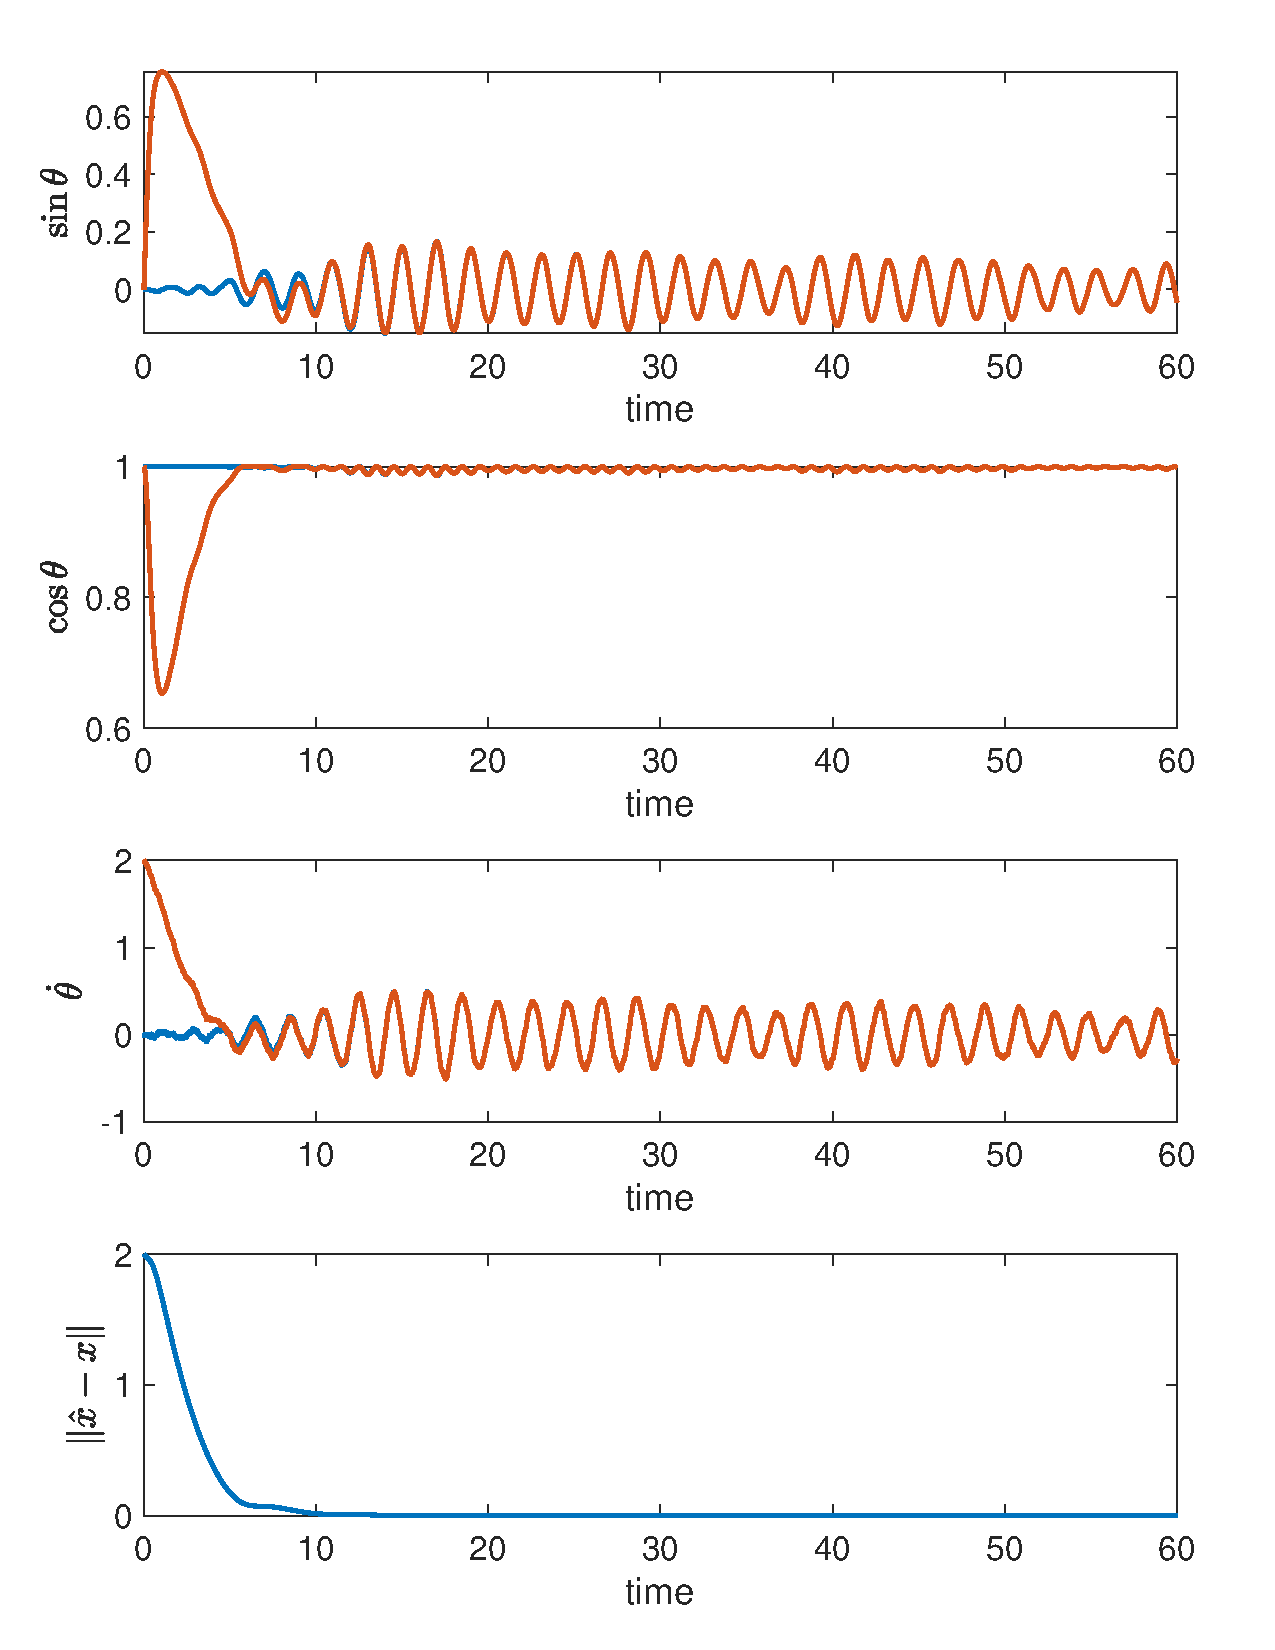
\includegraphics[width=0.8\linewidth]{images/pendulum-simulation-sos-observer} 

}

\caption{Simulation of the pendulum observer design from convex optimization}\label{fig:sos-observer-pendulum-simulation}
\end{figure}

\end{example}

\hypertarget{observer-feedback}{%
\section{Observer Feedback}\label{observer-feedback}}

Now that we have good ways to design a state observer, we will see how we can use the observer for feedback control.

\begin{example}[Pendulum Stabilization with A Luenberger Observer]
\protect\hypertarget{exm:pendulumLuenbergerFeedback}{}\label{exm:pendulumLuenbergerFeedback}

In Example \ref{exm:pendulumLuenberger}, we have written the dynamics of a pendulum, and the dynamics of a Luenberger observer as
\begin{align}
\dot{x} &= A x + B(u,y) \\
\dot{\hat{x}} &= A \hat{x} + B(u,y) + KC (x - \hat{x})
\end{align}
We wish to understand (so we can optimize) the behavior of this system under certain control input \(u\). To do so, let us denote \(e = \hat{x} - x\), and write the above dynamics as
\begin{align}
\dot{x} &= A x + B(u,Cx) \\
\dot{e} & = (A - KC) e
\end{align}
Denoting \(z = [x,e]^T\), we have the augmented dynamics
\[
\dot{z} = \underbrace{\begin{bmatrix} A & 0 \\ 0 & A - KC \end{bmatrix}}_{=:F} z + \underbrace{\begin{bmatrix} B(u,Dz) \\ 0 \end{bmatrix}}_{=:G(z,u)}
\]
We want to stabilize the system at \(z_0 = [\pi,0,0,0]^T\) (the upright position) subject to control bounds \(u \in \mathbb{U} = [-u_{\max},u_{\max}]\).

We need to find a control Lyapunov function (CLF), \(V(z)\), that satisfies the following constraints:
\[
    V(z_0) = 0
\]
\[
    V(z) > 0 \quad \forall z \in \{z: V(z) < \rho, z \neq z_0 \}
\]
\[
    \inf_{u \in \mathbb{U}} [L_F V(z) + L_G V(z)] \leq 0 \quad \forall z \in \mathcal{Z}
\]

where \(L_F V\) and \(L_G V\) are the Lie derivatives of \(V\) along \(F\) and \(G(z,u)\), respectively. \(\mathcal{Z}\) is the set of all possible augmented states. The CLF will define the set of admissible control inputs \(U\).
\[
    U = \{ u: L_f V(z) + L_g V(z)u \leq 0 \}
\]
To find the smallest-magnitude control input such that \(u \in K\), we may use a quadratic program:

\[
    \min_{u \in \mathcal{U}} ||u||^2
\]
\[
\mathrm{s.t.} \quad L_f V(z) + L_g V(z)u \leq -c V(z)
\]

where \(c\) is some positive constant. The challenge now is in choosing a suitable \(V(z)\).

\end{example}

\hypertarget{geometric-vision}{%
\chapter{Geometric Vision}\label{geometric-vision}}

In this Chapter, we introduce the fundamentals of \emph{geometric vision}, a (classical) branch of computer vision that seeks to estimate geometric models (e.g., 3D rotations, translations, and points) from sensor measurements (e.g., images and point clouds). There are two goals for introducing geometric vision.

\begin{enumerate}
\def\labelenumi{\arabic{enumi}.}
\item
  In the output feedback Chapter \ref{output-feedback}, we see that the full state \(x\) of a dynamical system is often not available, and needs to be estimated from the measurement signal \(y\) that satisfies
  \[
  y(t) = h(x(t),u(t))
  \]
  potentially plus some noise. In Chapter \ref{output-feedback}, we studied the case where \(y\) is part of the state \(x\), often the position \(q\) of a second-order system \(x=[q;\dot{q}]\). For example, in the pendulm swing-up example, we assume the angular position \(\theta\) is observed, but not the angular velocity \(\dot{\theta}\). However, in many practical applications, the measurement signal \(y\) does not directly tell us the position \(q\), and we need to estimate \(q\) from \(y\). For instance, a quadcopter needs to estimate its position from its onboard cameras. Once we obtain an estimated \(q\) from \(y\), we can use the observer synthesis methods in Chapter \ref{output-feedback} to obtain the full state estimation.
\item
  The estimation community and the control community are a bit separated (at least in my opinion), despite that they share a lot of common tools, especially \emph{optimization}. We will see that estimating \(q\) from \(y\), where \(y\) could be a high-dimensional image, is often formulated as an optimization problem that is difficult to solve. However, using the SOS tool we developed in Chapter \ref{stability}, we can actually solve the optimization problem to global optimality.
\end{enumerate}

\hypertarget{d-rotations-and-poses}{%
\section{3D Rotations and Poses}\label{d-rotations-and-poses}}

\hypertarget{rotation-matrices}{%
\subsection{Rotation matrices}\label{rotation-matrices}}

The first part is a quick recap of the basics in linear algebra.

\begin{definition}[Orthogonal Matrix]
\protect\hypertarget{def:orthogonalmatrix}{}\label{def:orthogonalmatrix}We call a \(n\times n\) square matrix \(A\) orthogonal if the column of \(A\) is orthogonal to each other and all the column vectors have unit length. The set of all \(n\times n\) orthogonal matrices is denoted as \(O(n)\).
\end{definition}

Below are some basic properties of orthogonal matrices:

\begin{proposition}[Property of Orthogonal Matrix]
\protect\hypertarget{prp:propertyoforthogonal}{}\label{prp:propertyoforthogonal}

Let \(A\) be a \(n\times n\) orthogonal matrix. Then:

\begin{enumerate}
\def\labelenumi{\arabic{enumi}.}
\item
  \(A^T = A^{-1}\) and \(A^T\) is also a orthogonal matrix.
\item
  For every orthogonal matrices \(A,B\), \(AB\) is also a orthogonal matrix.
\item
  \(\det(A) = \pm 1\).
\item
  \(A\) preserves dot product, i.e.~\(<x,y> = <Ax,Ay>\), thus preserves the length of a vector, i.e.~\(\|Ax\|_2 = \|x\|_2\).
\item
  All the eigenvalues of \(A\) have modulus one.
\end{enumerate}

\end{proposition}

\begin{proof}
We only offer the proof of the last property. Consider any eigenvalue \(\lambda\) of \(A\), and \(x\) be its eigenvector.
We have \(<x,x> = <A^TAx,x>=<Ax,Ax> = |\lambda|^2<x,x>\), thus \(|\lambda|=1\).
\end{proof}

There are two types of orthogonal matrices, categorized by determinant \(1\) and \(-1\). Those with determinant \(1\) are called rotation matrices. The set of rotation matrices is denoted as \(SO(n)\) (Special Orthogonal). In the world of robotics and most engineering fields, we care about \(SO(3)\) the most. Below are some basic properties of \(3\times 3\) rotation matrices:

\begin{proposition}[Property of Rotation Matrix]
\protect\hypertarget{prp:propertyofrotation}{}\label{prp:propertyofrotation}

Let \(A\) be a \(3\times 3\) orthogonal matrix. Then:

\begin{enumerate}
\def\labelenumi{\arabic{enumi}.}
\item
  \(\det(A) = \pm 1\)
\item
  For every rotation matrices \(A,B\), \(A^T\),\(AB\) are also rotation matrices.
\item
  \(A\) always has an eigenvalue \(1\). If \(A\) is not identity, \(A\) either has two conjugate complex eigenvalues not equal to 1, or has two eigenvalues -1.
\end{enumerate}

\end{proposition}

\begin{proof}
We can only prove the last property.

From the property of orthogonal matrix, we know that all eigenvalues have modulus one. First, note that there must exist at least one real eigenvalue. Because eigenvalues with nonzero imaginary parts always come in pair and 3 is an odd number.

Then there are two possible cases: (1) All the eigenvalues are real; (2) There is only one eigenvalue.

For case one, note that the determinant of a matrix is the product of all eigenvalues, then rotation matrix can't have all the eigenvalues -1.

For case two. The product of the pairing complex eigenvalues is the square of the modulus of the eigenvalue, which is 1. So the real eigenlvalue left must be 1.

Finally if all the eigenvalues of \(A\) are 1, then \(A\) must be identity.
\end{proof}

\hypertarget{coordinate-frame}{%
\subsection{Coordinate Frame}\label{coordinate-frame}}

\emph{Coordinate frames} are a set of orthogonal basis (containing three axes) attached to a certain body at a point. It serves as the tool to describe the position of points relative to that body. Conventionally, coordinate frames are right-handed. We will encounter different frames in applications, including: (1) Robot (robot frame ``\(r\)''), (2) Sensor on the robot (e.g.~camera frame `\(c\)'), (3) A fixed location in the world (world frame ``\(w\)'')

It's worth metion that, denote \(\vec{x},\vec{y},\vec{z}\) as the three axes of the coordinate frame, then the right-handed property can be expressed as: \(\vec{x}\cdot(\vec{y}\times \vec{z}) = 1\), which is the same as \(\det ([\vec{x},\vec{y},\vec{z}]) = 1\). So the matrix \([\vec{x},\vec{y},\vec{z}]\) is a rotation matrix.

It's natural for us to ask three questions: (1) How to express a point in a given frame? (2) How to represent a frame \(r\) with respect to a frame \(w\)? (3) How to translate the coordinate of a point in different frames?

\textbf{(1) How to express a point in a given frame?}

Let's consider a reference frame \(r\) and denote the the three axes attached to it as \(\vec{x^r},\vec{y^r},\vec{z^r}\). Then for any point \(p\), we care about the vector pointing from the origin of the frame to \(p\). We slightly abuse the notation and let that vector called \(p\).(Since we will only care about the vector) Then, we can express \(p\) as the combination of the basis, i.e.~\[p = p^r_x \vec{x^r}+p^r_y\vec{y^r}+p^r_z\vec{z^r} = \begin{bmatrix} \vec{x^r},\vec{y^r},\vec{z^r}\end{bmatrix} \begin{bmatrix} p^r_x\\p^r_y\\p^r_z \end{bmatrix}\] Thus we can fully describe point \(p\) with three scalars \(p^r_x,p^r_y,p^r_z\), which is called the coordinates of \(p\) with respect to the frame \(r\).

\textbf{(2) How to represent a frame \(r\) with respect to a frame \(w\)?}

Now we consider how to describe frame \(w\) in frame \(r\). Let's focus on the simple case where the origin of the two coordinate systems coincide. Then we can express the axes \(\vec{x^w},\vec{y^w},\vec{z^w}\) in frame \(r\) directly. For example, thanks to the orthogonality, we can get:\[\vec{x^w} = <\vec{x^w},\vec{x^r}>\vec{x^r} +<\vec{x^w},\vec{y^r}>\vec{y^r} +  <\vec{x^w},\vec{z^r}>\vec{z^r} = \begin{bmatrix}
    \vec{x^r},\vec{y^r},\vec{z^r}\end{bmatrix}\begin{bmatrix} <\vec{x^w},\vec{x^r}>\\ <\vec{x^w},\vec{y^r}>\\<\vec{x^w},\vec{z^r}>
\end{bmatrix}\] So we can get:
\[\begin{bmatrix}
    \vec{x^w},\vec{y^w},\vec{z^w}
\end{bmatrix} = \begin{bmatrix}
    \vec{x^r},\vec{y^r},\vec{z^r}
\end{bmatrix}\begin{bmatrix}
    &<\vec{x^w},\vec{x^r}> &<\vec{y^w},\vec{x^r}> &<\vec{z^w},\vec{x^r}>\\
    &<\vec{x^w},\vec{y^r}> &<\vec{y^w},\vec{y^r}> &<\vec{z^w},\vec{y^r}>\\
    &<\vec{x^w},\vec{z^r}> &<\vec{y^w},\vec{z^r}> &<\vec{z^w},\vec{z^r}>
\end{bmatrix} = \begin{bmatrix}
    \vec{x^r},\vec{y^r},\vec{z^r}
\end{bmatrix}R^r_w\]

Note that \(R^r_w = (\begin{bmatrix}  \vec{x^r},\vec{y^r},\vec{z^r} \end{bmatrix})^T\begin{bmatrix}  \vec{x^w},\vec{y^w},\vec{z^w} \end{bmatrix}\) is a rotation matrix.

\begin{example}[A simple example of translation between frames]
\protect\hypertarget{exm:frametransexample}{}\label{exm:frametransexample}If we for frame \(w\) we have \[\begin{bmatrix}
    \vec{x^w},\vec{y^w},\vec{z^w}
\end{bmatrix} = I_3\]
and for frame \(r\) we have \[\begin{bmatrix}
    \vec{x^r},\vec{y^r},\vec{z^r}
\end{bmatrix} = \begin{bmatrix}
    &\cos(\theta) &-\sin(\theta) &0\\
    &\sin(\theta) &\cos(\theta)  &0\\
    &0            &0             &1
\end{bmatrix}\]

Then we can have:

\begin{align}
\begin{bmatrix}
    \vec{x^w},\vec{y^w},\vec{z^w}
\end{bmatrix} =& \begin{bmatrix}
    \vec{x^r},\vec{y^r},\vec{z^r}
\end{bmatrix}\begin{bmatrix}
    &<\vec{x^w},\vec{x^r}> &<\vec{y^w},\vec{x^r}> &<\vec{z^w},\vec{x^r}>\\
    &<\vec{x^w},\vec{y^r}> &<\vec{y^w},\vec{y^r}> &<\vec{z^w},\vec{y^r}>\\
    &<\vec{x^w},\vec{z^r}> &<\vec{y^w},\vec{z^r}> &<\vec{z^w},\vec{z^r}>
\end{bmatrix} \\
  =& \begin{bmatrix}
    \vec{x^r},\vec{y^r},\vec{z^r}
\end{bmatrix}\begin{bmatrix}
    &\cos(\theta) &\sin(\theta) &0\\
    &-\sin(\theta) &\cos(\theta) &0\\
    &0 &0 &1
\end{bmatrix}
  \end{align}

So we can get \(R_w^r = \begin{bmatrix}  &\cos(\theta) &\sin(\theta) &0\\  &-\sin(\theta) &\cos(\theta) &0\\  &0 &0 &1 \end{bmatrix}\)
\end{example}

\textbf{(3) How to translate the coordinate of a point in different frames?}

First let us consider frame \(w\) and \(r\) with the same origin. Then for any point \(\vec{p}\), we will have:

\begin{align}
    &\vec{p} = \begin{bmatrix} \vec{x^r},\vec{y^r},\vec{z^r}\end{bmatrix} \begin{bmatrix} p^r_x\\p^r_y\\p^r_z \end{bmatrix} = \begin{bmatrix} \vec{x^w},\vec{y^w},\vec{z^w}\end{bmatrix} \begin{bmatrix} p^w_x\\p^w_y\\p^w_z \end{bmatrix} \\
    \Rightarrow& \vec{p^r} = \begin{bmatrix} p^r_x\\p^r_y\\p^r_z \end{bmatrix} = \begin{bmatrix} \vec{x^r}^T\\ \vec{y^r}^T\\ \vec{z^r}^T\end{bmatrix} \begin{bmatrix} \vec{x^w},\vec{y^w},\vec{z^w}\end{bmatrix} \begin{bmatrix} p^w_x\\p^w_y\\p^w_z \end{bmatrix} = R^r_w \begin{bmatrix} p^w_x\\p^w_y\\p^w_z \end{bmatrix} = R^r_w\vec{p^w} 
\end{align}

We can find that, we only need to multiply the matrix \(R^r_w\) to translate the coordinate in \(w\) frame to \(r\) frame.

\begin{example}[A simple example of translation between frames (Cont.)]
\protect\hypertarget{exm:frametransexamplecont}{}\label{exm:frametransexamplecont}If we for frame \(w\) we have \[\begin{bmatrix}
    \vec{x^w},\vec{y^w},\vec{z^w}
\end{bmatrix} = I_3\]
and for frame \(r\) we have \[\begin{bmatrix}
    \vec{x^r},\vec{y^r},\vec{z^r}
\end{bmatrix} = \begin{bmatrix}
    &\cos(\theta) &-\sin(\theta) &0\\
    &\sin(\theta) &\cos(\theta)  &0\\
    &0            &0             &1
\end{bmatrix}\]
Assume point \(p\) has coordinates \(\vec{p^w} = \begin{bmatrix} \cos(\theta)\\\sin(\theta)\\0 \end{bmatrix}\) in frame \(w\). Then we can have:
\[\vec{p^r} = R^r_w\vec{p^w} = \begin{bmatrix}
    &\cos(\theta) &\sin(\theta) &0\\
    &-\sin(\theta) &\cos(\theta) &0\\
    &0 &0 &1
\end{bmatrix}\begin{bmatrix} \cos(\theta)\\\sin(\theta)\\0 \end{bmatrix} = \begin{bmatrix} 1\\0\\0 \end{bmatrix}\]
\end{example}

What if the origin of the two frames are not the same? We may think of two ways to do so: (1) First do the translation, then do the rotation, (2) First do the rotation, then do the translation. The most natural way is (1). Here is a quick example:

\begin{example}[A simple example with different origins]
\protect\hypertarget{exm:translationex}{}\label{exm:translationex}\leavevmode

Suppose we have two frames: Frame 1 and Frame 2 as depicted below. All the coordinates are in frame 1. \[
    R_1^2 = \begin{bmatrix}<\vec{x^1},\vec{x^2}> &<\vec{y^1},\vec{x^2}> \\
    <\vec{x^1},\vec{y^2}> &<\vec{y^1},\vec{y^2}> \end{bmatrix} = \begin{bmatrix} \frac{\sqrt{2}}{2} &\frac{\sqrt{2}}{2} \\ -\frac{\sqrt{2}}{2} &\frac{\sqrt{2}}{2}\end{bmatrix}\] and \(t_1^2 = \begin{bmatrix} 0\\-2\end{bmatrix}\).

\begin{figure}

{\centering 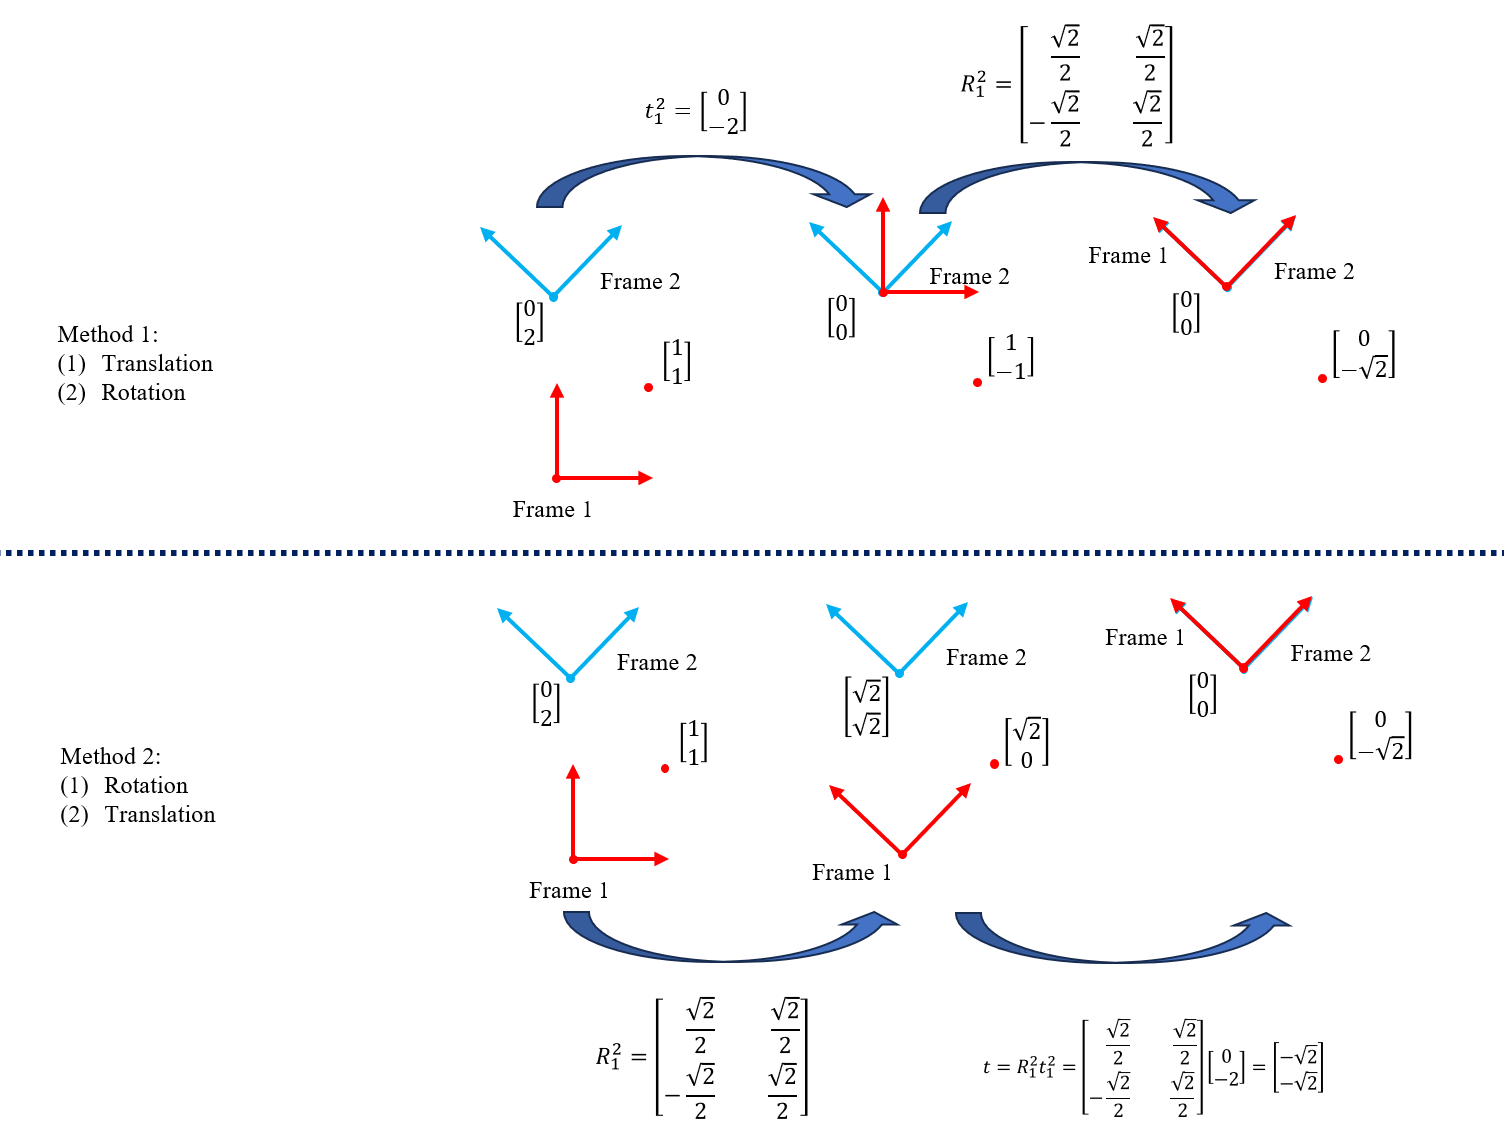
\includegraphics[width=1\linewidth]{images/translation_example} 

}

\caption{A simple example with different origins}\label{fig:translation-example}
\end{figure}

We can see that, if we want to use method 1, we can just consecutively do the translation and the rotation. However, if we want to do it reversely, we must multiply the translation by the rotation matrix. Actually it's easy to show this two methods are equivalent.

In conclusion, the formula is as follows:
\[p^2 = R^2_1(p^1+t_1^2) = R^2_1p^1+R^2_1t_1^2\]

\end{example}

\hypertarget{representations-of-the-rotations}{%
\subsection{Representations of the rotations}\label{representations-of-the-rotations}}

Although rotation matrix is enough to characterize a rotation. But it's not simple enough and not intuitive enough. For example, we can't explicitly know the rotation angles from the rotation matrix. The rotation matrix has 9 elements, but there are many constraints. So is it possible for us to find a simpler representation for rotation?

\hypertarget{euler-angles-representation}{%
\subsubsection{Euler angles representation}\label{euler-angles-representation}}

Intuitively, we can achieve any rotation by rotating along the x, y, z axes in turn. First let's introduce some basic rotations along x,y,z axes.

\begin{proposition}[Basic Rotations]
\protect\hypertarget{prp:basicrotation}{}\label{prp:basicrotation}

Below are the basic rotation matrices along the x, y, z axes, all the rotations are counterclockwise.

\begin{enumerate}
\def\labelenumi{\arabic{enumi}.}
\item
  Rotation along z axes, with angle \(\gamma\) is:
  \[\begin{bmatrix}
      &\cos(\gamma) &\sin(\gamma) &0\\
      &-\sin(\gamma) &\cos(\gamma) &0\\
      &0 &0 &1
  \end{bmatrix}\]
\item
  Rotation along y axes, with angle \(\beta\) is:
  \[\begin{bmatrix}
    &\cos(\beta) &0 &-\sin(\beta)\\
    &0 &1 &0\\
    &\sin(\beta) &0 &\cos(\beta)
  \end{bmatrix}\]
\item
  Rotation along x axes, with angle \(\alpha\) is:
  \[\begin{bmatrix}
    &1&0&0 \\
    &0 &\cos(\alpha) &\sin(\alpha)\\
    &0 &-\sin(\alpha) &\cos(\alpha)
  \end{bmatrix}\]
\end{enumerate}

\end{proposition}

Actually every rotation can be written into combination of no more than three basic rotations, with no two consecutive rotations along the same axis. A popular choice of the sequence is roll-pitch-yaw.

\begin{proposition}[Roll-pitch-yaw angle representation]
\protect\hypertarget{prp:roll-pitch-yaw}{}\label{prp:roll-pitch-yaw}Any rotation matrix \(R^w_r\) can be written into combination of basic rotations in the following order:\[R^w_r = R_z(\gamma)R_y(\beta)R_x(\alpha)\]
where \(\gamma\) is called the yaw angle, \(\beta\) is called the pitch angle, and \(\alpha\) is called the roll angle.
\end{proposition}

This representation is very intuitive, because it directly tells us the rotation angles. However, the calculation will include trigonometric functions. So it can be hard to calculate and analyze. Moreover, if you want to recover the Euler angles from
rotation matrices, there may be problems in certain point. The example below shows the singularities.

\begin{example}[Singularities for Euler angles]
\protect\hypertarget{exm:singulareuler}{}\label{exm:singulareuler}In formula \[R = R_z(\gamma)R_y(\beta)R_x(\alpha)\]
consider \(\beta = \frac{\pi}{2}\). Then we will have:
\[R = R_z(\gamma)R_y(\frac{\pi}{2})R_x(\alpha) = \begin{bmatrix}
    &0 &\sin(\alpha+\gamma) &-\cos(\alpha+\gamma)\\
    &0 &\cos(\alpha+\gamma)  &\sin(\alpha+\gamma)\\
    &1            &0             &0
\end{bmatrix}\]
So there are ambiguities in choosing \(\alpha,\gamma\) for the same rotation matrices.
\end{example}

\hypertarget{axis-angle-representation}{%
\subsubsection{Axis-angle representation}\label{axis-angle-representation}}

Another intuitive representation is the axis-angle representation. Imagine a rotation in 3D space, it seems that all the rotations are rotation with respect to an axis (not necessary to be aligned with the x,y,z axes) for some angle. How to find the axis and the corresponding angle?

Given rotation angle and axis, how can we get the rotation matrix? Next theorem will give us an explicit formula.

\begin{theorem}[Rodrigues' rotation formula]
\protect\hypertarget{thm:rodrigues}{}\label{thm:rodrigues}Given a rotation angle \(\theta\) and a rotation axis \(u\) (expressed by a unit vector). The rotation matrix \(R\) can be computed as: \[R = \cos(\theta)I_3+\sin(\theta)[u]_\times+(1-\cos(\theta))uu^T\]
where \([u]_\times = \begin{bmatrix}  &0 &-u_z &u_y\\  &u_z &0 &-u_x\\  &-u_y &u_x &0 \end{bmatrix}\)
\end{theorem}

How can we do it reversely? Intuitively, axis of the rotation is the direction that the rotation preserves. Mathematically speaking, axis of rotation is in the direction of the eigenvector with respect to the eigenvalue of 1. From the discussion above, if rotation is not equal to identity, then there is a unique direction of rotation axis. So we can solve for the rotation axis by calculating \(u\) satisfying:\[Ru = u\] To get the rotation angle, we notice that if we take trace of both of the sides of Rodrigues' rotation formula, we can get:\[\text{Tr}(R) = 2\cos(\theta) + 1\] Note that if we treat \(\theta\) as the minimal angle of the rotation, we can always restrict the \(\theta\in[0,\pi]\) and thus \(\theta = \arccos(\frac{\text{Tr}(R) - 1}{2})\). However, then we will leave the rotation direction to the sign of axis \(u\). That is to say: \(R(u,\theta)^{-1} = R(-u,\theta)\). So we need to double check the two potential solutions to make sure which rotation is the one we want.

\hypertarget{quaternion-representation}{%
\subsubsection{Quaternion representation}\label{quaternion-representation}}

W.R. Hamilton first introduced the definition of quaternion representation.

\begin{definition}[Quaternion]
\protect\hypertarget{def:quaternion}{}\label{def:quaternion}A quaternion is represented in the form \(\textbf{q} = \textbf{i}q_1 + \textbf{j}q_2 + \textbf{k}q_3 + q_4\), where \(q_1,q_2,q_3,q_4\) are real numbers and \(\bf i,j,k\) satisfying:
\begin{align}
  &\textbf{i}^2=\textbf{j}^2=\textbf{k}^2=-1\\
  &\textbf{ij} = -\textbf{ji} = \textbf{k} \quad \textbf{jk} = -\textbf{kj} = \textbf{i} \quad \textbf{ki} = -\textbf{ik} = \textbf{j}
 \end{align}
\end{definition}

We can also write the quaternion in the column vector form: \(\textbf{q} = \begin{bmatrix} q_1\\q_2\\q_3\\q_4 \end{bmatrix}\). We are particularly interested in \textbf{unit quaternions}, which means the column vector has unit length. Unit quaternions can represent rotations, actually we can get quaternions immediately from the axis-angle representation. The main idea is to use the axis-angle representation but in a more compact format. Concretely speaking, given rotation angle \(\theta\) and rotation axis \(u\)(in unit length), the corresponding unit quaternion is as follows: \[q = \begin{bmatrix}u\sin(\frac{\theta}{2}) \\ \cos(\frac{\theta}{2})\end{bmatrix}\]

The corresponding rotation matrix is:
\[R(q) = \begin{bmatrix} q_1^2 - q_2^2 - q_3^2 + q_4^2  &2(q_1q_2-q_3q_4) &2(q_1q_3 +q_2q_4)\\
2(q_1q_2+q_3q_4) & -q_1^2+q_2^2-q_3^2+q_4^2 &2(q_2q_3 - q_1q_4)\\
2(q_1q_3-q_2q_4) &2(q_2q_3+q_1q_4) &-q_1^2-q_2^2+q_3^2+q_4^2 \end{bmatrix}\]

Quaternion representation doesn't have singularities. But there is still a little ambiguity that \(q\) and \(-q\) always represent the same rotation, which means the quaternion is a double cover of the 3D rotation. Actually, quaternions also give us great convenience in calculation, because of its compact representation. For computational use, we care about: \textbf{(1)How to compose rotations? (2) How to take inverse for quaternions (3) How to rotate a 3D vector using quaternions?}

\textbf{(1)How to compose rotations? }

Consider two quaternions \(q_a = q_{a,1}i +q_{a,2}j +q_{a,3}k +q_{a,4},\  q_b = q_{b,1}i +q_{b,2}j +q_{b,3}k +q_{b,4}\). Then the composition of the corresponding rotation is just the product of two quaternions. Explicitly,
\begin{align}
q_c = q_a\otimes q_b =& (q_{a,4}q_{b,1} -q_{a,3}q_{b,2} + q_{a,2}q_{b,3} + q_{a,1}q_{b,4})i \\
+& (q_{a,3}q_{b,1} +q_{a,4}q_{b,2} - q_{a,1}q_{b,3} + q_{a,2}q_{b,4})j \\
+& (-q_{a,2}q_{b,1} +q_{a,1}q_{b,2} + q_{a,4}q_{b,3} + q_{a,3}q_{b,4})k \\
+& (-q_{a,1}q_{b,1} -q_{a,2}q_{b,2} - q_{a,3}q_{b,3} + q_{a,4}q_{b,4})
\end{align}

If we use vector to represent quaternion, we can claim the following formula:

\[ q_c = \begin{bmatrix} q_{a,4} & -q_{a,3} & q_{a,2} & q_{a,1}\\
q_{a,3} & q_{a,4} &-q_{a,1} &q_{a,2} \\
-q_{a,2} & q_{a,1} & q_{a,4} &q_{a,3} \\
-q_{a,1} & -q_{a,2} & -q_{a,3} &q_{a,4}\end{bmatrix} \begin{bmatrix} q_{b,1}\\q_{b,2}\\q_{b,3}\\q_{b,4}\end{bmatrix} \] Similar formula can be derived for \(q_a\).

\textbf{(2) How to take inverse for quaternions?}

Assume that now we have the pose of frame \(r\) with respect to a frame \(w\), i.e.~we know \(q_r^w\). How can we get the opposite, i.e.~the pose of frame \(w\) with respect to frame \(r\)? The answer is to take the inverse of the rotation. It's easy to carry out using rotation matrix, but how shall we proceed using quaternions? Let's remind ourselves that quaternion is nothing but rearranged axis-angle representation. So naturally the inverse is as follows:
\[q_w^r = \begin{bmatrix}-u_r^w\sin(\frac{\theta}{2}) \\ \cos(\frac{\theta}{2})\end{bmatrix} = (q_r^w)^{-1}\]
This process is also compatible with the quaternion product.

\textbf{(3) How to rotate a 3D vector using quaternions?}

One key question is, given coordinates in one frame, and the pose of that frame in another frame, how can we translate the coordinates? Assume there is a point \(p\), and we know its coordinates in frame \(r\), denoted as \(p^r\). Also we know the pose of frame \(r\) in frame \(w\), denoted as \(q_r^w\). For simplicity, we assume that the two frame share the same origin. How can we get the coordinates of \(p\) with respect to the frame \(w\), i.e.~\(p^w\)? We have the following formula:
\[p^w = (q^w_r)\otimes\begin{bmatrix} p^r\\1\end{bmatrix}\otimes(q^w_r)^{-1} = \begin{bmatrix} R^w_rp^r\\1\end{bmatrix}\]
i.e.~we can compute the rotation by first stack an extra entry 1 at the end of \(p^r\), then let \(q^w_r\) act `conjugately' on it.

\hypertarget{miscellaneous-topics-on-rotations}{%
\subsection{Miscellaneous topics on rotations}\label{miscellaneous-topics-on-rotations}}

\hypertarget{lie-group-structure-of-rotations}{%
\subsubsection{Lie group structure of rotations}\label{lie-group-structure-of-rotations}}

Actually, on one hand, the set of rotation matrices (\(SO(3)\)) is closed under matrix multiplication (and some other properties), which gives rise to its algebraic structure (which is called `group'). On the other hand, the set of rotation matrices has its own topological structure (which is called `manifold'). Lie group is both group and smooth manifold, but we'll not introduce Lie group formally.

Geometrically, thanks to the quaternion representation, we can treat the group \(SO(3)\) as a sphere in 4D, but due to \(R(q) = R(-q)\), we must image there are portals connecting the antipodal points. Locally we can just think it as a sphere. For a sphere, we can imagine that at each point there is a tangent space. The tangent space at the identity is called Lie algebra. Why identity? There is nothing special with identity, just because: (1) Every group has identity. (2) The tangent space at other points can be obtained from identity. Lie algebra is deeply connected with Lie group. Imagine the sphere case, the sphere itself is curved, but we can use coordinates to translate the sphere into a flat map. Lie algebra is a flat space which we can make use of to study about the complicated curved Lie group. We will have some intuition on it by examining \(SO(3)\).

\begin{figure}

{\centering \includegraphics[width=1\linewidth]{images/sphere} 

}

\caption{Sphere and tangent space}\label{fig:sphere}
\end{figure}

Lie group \(SO(3)\) is related to its Lie algebra \(\mathfrak{so}(3)\). We will state without proof that the Lie algebra \(\mathfrak{so}(3)\) is the set of \(3\times 3\) skew symmetric matrices.

\textbf{Exponential Map and Logarithm Map:}

Looking at the sphere in the picture, it seems natural for us to bridge the endpoint of the green curved line, which is still on the sphere, with the endpoint of the red line, which is in the tangent space. This retraction is called exponential map. For matrix Lie group (including \(SO(3)\)), the exponential map coinsides with the matrix exponential (See \ref{linear-algebra}.)

We will check this on the \(SO(3)\) case:

\begin{theorem}[Matrix exponential for rotations]
\protect\hypertarget{thm:matrixexprotation}{}\label{thm:matrixexprotation}The exponential map \(\text{exp:}\mathfrak{so}(3)\to SO(3)\) is well-defined.
\end{theorem}

\begin{proof}
Consider a \(3\times 3\) skew symmetric matrix \(A = \begin{bmatrix} 0 &-c &b\\c &0 &-a\\-b &a &0 \end{bmatrix}\), define \(w = \begin{bmatrix} a\\b\\c \end{bmatrix}, \hat{w} = w/\|w\|, \theta=\|w\|\). Then \(A = w_\times\). Consider \(\hat{w}_\times\), using the properties of the cross product, we have:\(\hat{w}^3_\times = -\hat{w}_\times\). Thus we can know that:
\begin{align}
    \exp(A) &= I + (1-\frac{\theta^3}{3!}+\frac{\theta^5}{5!}+\dots)\hat{w}_\times + (\frac{\theta^2}{2!}-\frac{\theta^4}{4!}+\frac{\theta^6}{6!})\hat{w}_\times^2\\
    &= I + \frac{\sin\theta}{\theta}A + \frac{1-\cos\theta}{\theta^2}A^2
  \end{align}
which actually coincide with the Rodrigues' formula. Thus \(\exp(A)\) is a rotation matrix.
\end{proof}

Actually the exponential map for \(SO(3)\) is surjective. From the derivation above, I believe we can see the similarity of this with the axis-angle representation. In order to map backwards, we want to recover the angle and the axis from the rotation matrix. There are infinitely many possible points due to the periodic property of trigonometric functions. So we may restrict the rotation angle \(\theta \in [0,\pi)\)。 Then from the derivation of the axis-angle representation, we can get:
\begin{align}
  \theta &= \arccos(\frac{\text{Tr}(R) - 1}{2})
\end{align}
Next is to recover the axis. Note that the whole space of \(n\times n\) matrices is the direct sum of \(n\times n\) symmetric matrices and \(n\times n\) skew symmetric matrices. So we can decompose the rotation matrix into symmetric and skew symmetric parts. From the formula above, we can decompose as:
\[ \exp(A) = \underbrace{\frac{\sin\theta}{\theta}A}_{\text{skew symmetric}} + \underbrace{I + \frac{1-\cos\theta}{\theta^2}A^2}_{\text{symmetric}}
\]
Thus we can recover the skew symmetric matrix \(A\) (the axis) by taking the skew symmetric part of \(\exp(A)\). Concretely, we can get: \(A = \frac{\theta}{2\sin\theta}(R - R^T)\).

Next we will give an example of how to use exponential map and logarithm map to do interpolation of rotations. Suppose we have two rotations \(R_1,R_2\), and we want to find a rotation \(R\) that is in between. We can use the following formula:
\[R = R_1\exp(\lambda\log(R_1^TR_2))\]
where \(\lambda\in[0,1]\).

\hypertarget{the-pinhole-camera-model}{%
\section{The Pinhole Camera Model}\label{the-pinhole-camera-model}}

Next let's take a look at the pinhole camera model, which is the simplest one. In this model, the picture in 2D is the projection of the corresponding 3D points with respect to the optical center.

\begin{figure}

{\centering \includegraphics[width=1\linewidth]{images/pinhole_camera} 

}

\caption{Pinhole Camera Model}\label{fig:pinhole-model}
\end{figure}

Consider point \(p\) in the camera frame. Suppose the focal length(i.e.~the distance from the optical center to the image plane) is \(f\). Then the coordinates of the projection of \(p\) is:
\[p_m^c = \begin{bmatrix} u_m^c\\v_m^c \end{bmatrix} = \begin{bmatrix} f\frac{p^c_x}{p^c_z}\\ f\frac{p^c_y}{p^c_z} \end{bmatrix}\]
The unit of these coordinates are meter. We would prefer to write the formula into a matrix form, but the barrier here is the quotient. In order to overcome this, we introduce \textbf{homogeneous coordinates}. In homogeneous coordinates system, if coordinates are multiplied by a non-zero scalar then the resulting coordinates represent the same point. We will add an extra entry to better represent this equivalence. Denote \[\tilde{p^c} = \begin{bmatrix} p_x^c\\p_y^c\\p_z^c\\1 \end{bmatrix}\]
Then the equivalence can be expressed as \[\forall k\neq0  \text{,}\quad \ \begin{bmatrix} p_x^c\\p_y^c\\p_z^c\\1 \end{bmatrix} \sim \begin{bmatrix} kp_x^c\\kp_y^c\\kp_z^c\\k \end{bmatrix}\]
With this notation, the projection equation can be written as: \[p^c_z\begin{bmatrix} u_m^c\\v_m^c\\1 \end{bmatrix} = \begin{bmatrix} f &0 &0 \\ 0 &f &0\\ 0 &0 &1\end{bmatrix} \begin{bmatrix} 1 &0 &0 &0 \\ 0 &1 &0 &0\\ 0 &0 &1 &0\end{bmatrix} \begin{bmatrix} p_x^c\\p_y^c\\p_z^c\\1 \end{bmatrix}\]

Normally when we deal with points in a 2D picture, we will prefer the unit is in pixels instead of meters. Next we will show how to convert the coordinates into pixels. In convention, the origin of the pixel coordinates is at the top-left of the image. So that we can express the coordinates in pixel as follows:
\[\begin{bmatrix} u^I\\v^I\\1 \end{bmatrix} = \begin{bmatrix} s_x &0 &o_x \\ 0 &s_y &o_y\\ 0 &0 &1\end{bmatrix} \begin{bmatrix} u_m^c\\v_m^c\\1 \end{bmatrix}\]
where \(s_x\) is the number of horizontal pixels per meter, \(s_y\) is the number of vertical pixels per meter, and \(\begin{bmatrix} o_x\\o_y\end{bmatrix}\) is the coordinates of the optical center.

Combing the previous result, we can get:
\begin{align} p_z^c\begin{bmatrix} u^I\\v^I\\1 \end{bmatrix} =& \begin{bmatrix} s_x &0 &o_x \\ 0 &s_y &o_y\\ 0 &0 &1\end{bmatrix} \begin{bmatrix} f &0 &0 \\ 0 &f &0\\ 0 &0 &1\end{bmatrix} \begin{bmatrix} 1 &0 &0 &0 \\ 0 &1 &0 &0\\ 0 &0 &1 &0\end{bmatrix} \begin{bmatrix} p_x^c\\p_y^c\\p_z^c\\1 \end{bmatrix} \\
=&  \underbrace{\begin{bmatrix} s_xf &0 &o_x \\ 0 &s_yf &o_y\\ 0 &0 &1\end{bmatrix}}_{K} \begin{bmatrix} 1 &0 &0 &0 \\ 0 &1 &0 &0\\ 0 &0 &1 &0\end{bmatrix} \begin{bmatrix} p_x^c\\p_y^c\\p_z^c\\1 \end{bmatrix}\end{align}
where \(K\) is called intrinsic matrix.

Notice that, in our derivation above, the homogeneous coordinates of \(p\) is in the camera frame. However, it's not always easy to know the coordinates in the camera frame. For example, sometimes we may have many different camera views, or the camera itself is moving. What we usually have is the coordinate of the 3D points in the world frame. Therefore we will add a procedure to transform the coordinates from world fram to the camera frame. From the previous section, we can know that we just need to do some rotations and translations. Therefore we can obtain the formula:
\begin{align} p_z^c\begin{bmatrix} u^I\\v^I\\1 \end{bmatrix} 
=&  \begin{bmatrix} s_xf &0 &o_x \\ 0 &s_yf &o_y\\ 0 &0 &1\end{bmatrix} \begin{bmatrix} 1 &0 &0 &0 \\ 0 &1 &0 &0\\ 0 &0 &1 &0\end{bmatrix} \begin{bmatrix} R_w^c &t^c_w \\ 0 &1 \end{bmatrix}\begin{bmatrix} p_x^w\\p_y^w\\p_z^w\\1 \end{bmatrix}\\
=& \begin{bmatrix} s_xf &0 &o_x \\ 0 &s_yf &o_y\\ 0 &0 &1\end{bmatrix} \begin{bmatrix} R_w^c &t^c_w\end{bmatrix}\begin{bmatrix} p_x^w\\p_y^w\\p_z^w\\1 \end{bmatrix}
\end{align}
where the matrix \(\begin{bmatrix} R_w^c &t^c_w\end{bmatrix}\) is called the extrinsic matrix.

Some pinhole cameras will introduce significant distortion to images. For cameras with wide field of view (FOV), they often suffers from radial distortion. Radial distortion makes straight lines look curved in the image. The farther points are from the center of the image, the larger the radial distortion will be. Radial distortion is primarily dominated by low-order components. An easy model of the distortion (in camera frame) is:

\[u^c = (1+K_1r^2+K_2r^4)u^c_{\text{distort}}\quad\quad v^c = (1+K_1r^2+K_2r^4)v^c_{\text{distort}}\]
where \((u^c,v^c)\) is the undistorted image point, \((u^c_{\text{distort}},v^c_{\text{distort}})\) is the distorted image point, \(r^2=(u^c_{\text{distort}})^2 +(v^c_{\text{distort}})^2\), and the \(K_n\) is the n-th distortion coefficient.

If we want to express in the image frame, we can obtain the following model:
\[u^I = (1+K_1r^2+K_2r^4)(u^I_{\text{distort}}-o_x)+o_x\quad\quad v^I = (1+K_1r^2+K_2r^4)(v^I_{\text{distort}}-o_y)+o_y\]
where \(r^2=(u^I_{\text{distort}}-o_x)^2 +(v^I_{\text{distort}}-o_y)^2\).

It's worth to mention that despite the radial distortion, there is another distortion called tangential distortion, which will not be elaborated here.

We often assume that the intrinsics of the camera and he distortion coefficients are already known from the previous camera calibration process, i.e.~we always assume that the camera is calibrated.

There are many existing codes and toolbox by hand if we want to undistort the pictures. Such as OpenCV has undistort function, and Matlab has undistortImage function. They can take in distorted images and return the undistorted ones.

\hypertarget{camera-pose-estimation}{%
\section{Camera Pose Estimation}\label{camera-pose-estimation}}

Suppose now we have a calibrated camera, but we don't know the rotation and translation, i.e.~the pose of the camera. We wish to find the extrinsics. Now what we have is a set of \(n\) 3D points and their corresponding 2D image projections. We wish to estimate the pose of the camera from these corresponding points.

\hypertarget{the-p3p-problem}{%
\subsection{The P3P Problem}\label{the-p3p-problem}}

Let's start from something simple. Consider there are three points \(P_1^w,P_2^w,P_3^w\) in the world frame, and their corresponding projection points on the image plane \(P^c_{m,1},P^c_{m,2},P^c_{m,3}\). The problem is: Can we found the coordinates of the points \(P_1,P_2,P_3\) in the camera frame? We will introduce a direct way to tackle the problem, called Grunert's method.

\begin{figure}

{\centering \includegraphics[width=1\linewidth]{images/P3P} 

}

\caption{P3P problem}\label{fig:p3p}
\end{figure}

From the coordinates of \(P^c_{m,1},P^c_{m,2},P^c_{m,3}\) in the image plane, we can calculate the angles between \(P_1,P_2,P_3\). Denote the angle between \(P_1,P_2\) as \(\gamma\), the angle between \(P_2,P_3\) as \(\beta\), and the angle between \(P_1,P_3\) as \(\alpha\). Remember that if \(P^c_{m,i} = \begin{bmatrix}u_{m,i}^c\\v^c_{m,i}\\1\end{bmatrix}\), then the camera frame coordinates \(P^c_i = \frac{s_i}{\sqrt{1+(u_{m,i}^c)^2+(v_{m,i}^c)^2}}\begin{bmatrix}u_{m,i}^c\\v_{m,i}^c\\1\end{bmatrix}\). So what we have to do is to solve for \(s_i\), which is the distance from the origin to the point \(P_i\).

Using law of cosines, we can obtain:

\begin{align}
  s_1^2 +s_2^2 - 2s_1s_2\cos\gamma = c^2\\
  s_1^2 +s_3^2 - 2s_1s_3\cos\beta = b^2\\
  s_2^2 +s_3^2 - 2s_2s_3\cos\alpha = a^2\\
\end{align}

Then if we let \(s_2 = us_1,s_3 = vs_1\), we can obtain:
\begin{align}
  s_1^2 = \frac{c^2}{1+u^2-2u\cos\gamma}\\
  s_1^2= \frac{b^2}{1+v^2-2v\cos\beta}\\
  s_1^2= \frac{a^2}{v^2+u^2-2uv\cos\alpha}\\
\end{align}
Then we can get:
\[
u^2-\frac{c^2}{b^2} v^2+2 v \frac{c^2}{b^2} \cos \beta-2 u \cos \gamma+\frac{b^2-c^2}{b^2}=0
\]
and
\[
u^2+\frac{b^2-a^2}{b^2} v^2-2 u v \cos \alpha+\frac{2 a^2}{b^2} v \cos \beta-\frac{a^2}{b^2}=0
\]
Then substituting the later equation back to the former one, we can express \(u\) in terms of \(v\). Then plug this into the latter equality, we can finally get an equation:
\[
A_4 v^4+A_3 v^3+A_2 v^2+A_1 v+A_0=0
\]
where

\begin{align}
& A_4=\left(\frac{a^2-c^2}{b^2}-1\right)^2-\frac{4 c^2}{b^2} \cos ^2 \alpha \\
& A_3=4\left[\frac{a^2-c^2}{b^2}\left(1-\frac{a^2-c^2}{b^2}\right) \cos \beta-\left(1-\frac{a^2+c^2}{b^2}\right) \cos \alpha \cos \gamma+2 \frac{c^2}{b^2} \cos ^2 \alpha \cos \beta\right] \\
& A_2=2[\left(\frac{a^2-c^2}{b^2}\right)^2-1+2\left(\frac{a^2-c^2}{b^2}\right)^2 \cos ^2 \beta+2\left(\frac{b^2-c^2}{b^2}\right) \cos ^2 \alpha \\
& -4\left(\frac{a^2+c^2}{b^2}\right) \cos \alpha \cos \beta \cos \gamma+2\left(\frac{b^2-a^2}{b^2}\right) \cos ^2 \gamma] \\
& A_1=4\left[-\left(\frac{a^2-c^2}{b^2}\right)\left(1+\frac{a^2-c^2}{b^2}\right) \cos \beta+\frac{2 a^2}{b^2} \cos ^2 \gamma \cos \beta-\left(1-\left(\frac{a^2+c^2}{b^2}\right)\right) \cos \alpha \cos \gamma\right] \\
& A_0=\left(1+\frac{a^2-c^2}{b^2}\right)^2-\frac{4 a^2}{b^2} \cos ^2 \gamma
\end{align}

From this equation, we can obtain up to four solutions. With each \(v\) we can obtain the corresponding \(u\) and thus all the other parameters. To eliminate the ambiguity, we can use a 4th point to confirm which one is the right solution.

\hypertarget{the-pnp-problem}{%
\subsection{The PnP Problem}\label{the-pnp-problem}}

\hypertarget{global-optimality}{%
\subsection{Global Optimality}\label{global-optimality}}

\hypertarget{handling-outliers}{%
\subsection{Handling Outliers}\label{handling-outliers}}

\hypertarget{point-cloud-registration}{%
\section{Point Cloud Registration}\label{point-cloud-registration}}

\hypertarget{adaptivecontrol}{%
\chapter{Adaptive Control}\label{adaptivecontrol}}

\hypertarget{model-reference-adaptive-control}{%
\section{Model-Reference Adaptive Control}\label{model-reference-adaptive-control}}

Basic flow for designing an adaptive controller

\begin{enumerate}
\def\labelenumi{\arabic{enumi}.}
\item
  Design a control law with variable parameters
\item
  Design an adaptation law for adjusting the control parameters
\item
  Analyze the convergence of the closed-loop system
\end{enumerate}

The control law design at the first step typically requires the designer to know what a good controller is if the true parameters were actually known, e.g., from feedback linearization (Appendix \ref{feedbacklinearization}), sliding control (Appendix \ref{slidingcontrol}) etc.

The design of the adaptation law typically comes from analyzing the dynamics of the tracking error, which as we will see often appears in the form of Lemma \ref{lem:adaptivecontrolbasic}.

The convergence of the closed-loop system is usually analyzed with the help of a Lyapunov-like function introduced in Chapter \ref{stability}.

\begin{lemma}[Basic Lemma]
\protect\hypertarget{lem:adaptivecontrolbasic}{}\label{lem:adaptivecontrolbasic}Let two signals \(e(t)\) and \(\phi(t)\) be related by
\begin{equation}
e(t) = H(p)[k \phi(t)^T v(t)]
\label{eq:acbasiclemmaephi}
\end{equation}
where \(e(t)\) a scalar output signal, \(H(p)\) a strictly positive real (SPR) transfer function, \(k\) an unknown real number with known sign, \(\phi(t) \in \mathbb{R}^m\) a control signal, and \(v(t) \in \mathbb{R}^m\) a measurable input signal.

If the control signal \(\phi(t)\) satisfies
\begin{equation}
\dot{\phi}(t) = - \mathrm{sgn}(k) \gamma e(t) v(t)
\label{eq:acbasiclemmaphilaw}
\end{equation}
with \(\gamma > 0\) a positive constant, then \(e(t)\) and \(\phi(t)\) are globally bounded. Moreover, if \(v(t)\) is bounded, then
\[
\lim_{t \rightarrow \infty} e(t) = 0.
\]
\end{lemma}

\begin{proof}
Let the state-space representation of \eqref{eq:acbasiclemmaephi} be
\begin{equation}
\dot{x} = A x + b [k \phi^T v], \quad e = c^T x.
\label{eq:acbasiclemmastatespace}
\end{equation}
Since \(H(p)\) is SPR, it follows from the Kalman-Yakubovich Lemma \ref{lem:KalmanYakubovich} that there exist \(P,Q \succ 0\) such that
\[
A^T P + P A = -Q, \quad Pb = c.
\]
Let
\[
V(x,\phi) = x^T P x + \frac{|k|}{\gamma} \phi^T \phi,
\]
clearly \(V\) is positive definite (i.e., \(V(0,0)=0\), and \(V(x,\phi) > 0\) for all \(x \neq 0, \phi \neq 0\)). The time derivative of \(V\) along the trajectory defined by \eqref{eq:acbasiclemmastatespace} with \(\phi\) chosen as in \eqref{eq:acbasiclemmaphilaw} is
\begin{align}
\dot{V} & = \frac{\partial V}{\partial x} \dot{x} + \frac{\partial V}{\partial \phi} \dot{\phi} \\
&= x^T (PA + A^T P) x + 2 x^T P b (k \phi^T v) + \frac{2|k|}{\gamma} \phi^T (- \mathrm{sgn}(k) \gamma e v) \\
& = - x^T Q x + 2 (x^T c)(k\phi^T v) - 2 \phi^T (e v) \\
& = - x^T Q x \leq 0.
\end{align}
As a result, we know \(x\) and \(\phi\) must be bounded (\(V(x(t),\phi(t)) \leq V(x(0),\phi(0))\) is bounded). Since \(e = c^T x\), we know \(e\) must be bounded as well.

If the input signal \(v\) is also bounded, then \(\dot{x}\) is bounded as seen from \eqref{eq:acbasiclemmastatespace}. Because \(\ddot{V} = -2x^T Q \dot{x}\) is now bounded, we know \(\dot{V}\) is uniformly continuous. Therefore, by Barbalat's stability certificate (Theorem \ref{thm:BarbalatStability}), we know \(\dot{V}\) tends to zero as \(t\) tends to infinity, which implies \(\lim_{t \rightarrow \infty} x(t) = 0\) and hence \(\lim_{t \rightarrow \infty} e(t) = 0\).
\end{proof}

\hypertarget{first-order-systems}{%
\subsection{First-Order Systems}\label{first-order-systems}}

Consider the first-order single-input single-output (SISO) system
\begin{equation}
\dot{x} = - a x + b u
\label{eq:ac-first-linear}
\end{equation}
where \(a\) and \(b\) are unknown groundtruth parameters. However, we do assume that the sign of \(b\) is known. {What if the sign of \(b\) is unknown too?}

Let \(r(t)\) be a reference trajectory, e.g., a step function or a sinusoidal function, and \(x_d(t)\) be a desired system trajectory that tracks the reference
\begin{equation}
\dot{x}_d = - a_d x_d + b_d r(t),
\label{eq:ac-first-linear-desired}
\end{equation}
where \(a_d,b_d > 0\) are user-defined constants. Note that the transfer function from \(r\) to \(x_d\) is
\[
x_d = \frac{b_d}{p + a_d} r
\]
and the system is stable. {Review basics of transfer function.}

The goal of adaptive control is to design a control law and an adaptation law such that the tracking error of the system \(x(t) - x_d(t)\) converges to zero.

\textbf{Control law}. We design the control law as
\begin{equation}
u = \hat{a}_r(t) r + \hat{a}_x(t) x 
\label{eq:ac-first-linear-control}
\end{equation}
where \(\hat{a}_r(t)\) and \(\hat{a}_x(t)\) are time-varying feedback gains that we wish to adapt. The closed-loop dynamics of system \eqref{eq:ac-first-linear} with the controller \eqref{eq:ac-first-linear-control} is
\[
\dot{x} = - a x + b (\hat{a}_r r + \hat{a}_x x) = - (a - b \hat{a}_x) x + b \hat{a}_r r. 
\]
With the equation above,
the reason for choosing the control law \eqref{eq:ac-first-linear-control} is clear: if the system parameters \((a,b)\) were known, then choosing
\begin{equation}
a_r^\star = \frac{b_d}{b}, \quad a_x^\star = \frac{a - a_d}{b}
\label{eq:ac-first-linear-optimal-gain}
\end{equation}
leads to the closed-loop dynamics \(\dot{x} = - a_d x + b_d r\) that is exactly what we want in \eqref{eq:ac-first-linear-desired}.

However, in adaptive control, since the true parameters \((a,b)\) are not revealed to the control designer, an adaptation law is needed to dynamically adjust the gains \(\hat{a}_r\) and \(\hat{a}_x\) based on the tracking error \(x(t) - x_d(t)\).

\textbf{Adaptation law}. Let \(e(t) = x(t) - x_d(t)\) be the tracking error, and we develop its time derivative
\begin{align}
\dot{e} &= \dot{x} - \dot{x}_d \\
        &= - a_d (x - x_d) + (a_d - a + b\hat{a}_x)x + (b \hat{a}_r - b_d) r \\
        & = - a_d e + b\underbrace{(\hat{a}_x - \hat{a}_x^\star)}_{=:\tilde{a}_x} x + b \underbrace{(\hat{a}_r - \hat{a}_r^\star )}_{=:\tilde{a}_r} r \\
        & = - a_d e + b (\tilde{a}_x x + \tilde{a}_r r) \label{eq:ac-first-linear-error-dynamics}
\end{align}
where \(\tilde{a}_x\) and \(\tilde{a}_r\) are the gain errors w.r.t. the optimal gains in \eqref{eq:ac-first-linear-optimal-gain} if the true parameters were known. The error dynamics \eqref{eq:ac-first-linear-error-dynamics} is equivalent to the following transfer function
\begin{equation}
e = \frac{1}{p + a_d} b(\tilde{a}_x x + \tilde{a}_r r) = \frac{1}{p + a_d} \left(b 
\begin{bmatrix} \tilde{a}_x \\ \tilde{a}_r \end{bmatrix}^T 
\begin{bmatrix} x \\ r \end{bmatrix}
\right),
\label{eq:ac-first-linear-error-dynamics-transfer}
\end{equation}
which is in the form of \eqref{eq:acbasiclemmaephi}. Therefore, we choose the adaptation law
\begin{equation}
\begin{bmatrix} \dot{\tilde{a}}_x \\ \dot{\tilde{a}}_r \end{bmatrix} = - \mathrm{sgn}(b) \gamma e \begin{bmatrix} x \\ r \end{bmatrix}.
\label{eq:ac-first-linear-adaptation-law}
\end{equation}

\textbf{Tracking convergence}. With the control law \eqref{eq:ac-first-linear-control} and the adaptation law \eqref{eq:ac-first-linear-adaptation-law}, we can prove that the tracking error converges to zero, using Lemma \ref{lem:adaptivecontrolbasic}. With \(\tilde{a}=[\tilde{a}_x, \tilde{a}_r]^T\), let
\begin{equation}
V(e,\tilde{a}) = e^2 + \frac{|b|}{\gamma} \tilde{a}^T \tilde{a}
\label{eq:ac-first-linear-lyapunov}
\end{equation}
be a positive definite Lyapunov function candidate with time derivative
\[
\dot{V} = - 2a_d e^2 \leq 0.
\]
Clearly, \(e\) and \(\tilde{a}\) are both bounded. Assuming the reference trajectory \(r\) is bounded, we know \(x_d\) is bounded (due to \eqref{eq:ac-first-linear-desired}) and hence \(x\) is bounded (due to \(e = x - x_d\) being bounded). Consequently, from the error dynamics \eqref{eq:ac-first-linear-error-dynamics} we know \(\dot{e}\) is bounded, which implies \(\ddot{V} = -4a_d e \dot{e}\) is bounded and \(\dot{V}\) is uniformly continuous. By Barbalat's stability certificate \ref{thm:BarbalatStability}, we conlude \(e(t) \rightarrow 0\) as \(t \rightarrow \infty\).

It is always better to combine mathematical analysis with intuitive understanding. Can you explain intuitively why the adaptation law \eqref{eq:ac-first-linear-adaptation-law} makes sense? (Hint: think about how the control should react to a negative/positive tracking error.)

\textbf{Parameter convergence}. We have shown the control law \eqref{eq:ac-first-linear-control} and the adaptation law \eqref{eq:ac-first-linear-adaptation-law} guarantee to track the reference trajectory. However, is it guaranteed that the gains of the controller \eqref{eq:ac-first-linear-control} also converge to the optimal gains in \eqref{eq:ac-first-linear-optimal-gain}?

We will now show that the answer is indefinite and it depends on the reference trajectory \(r(t)\). Because the tracking error \(e\) converges to zero, and \(e\) is the output of a stable filter \eqref{eq:ac-first-linear-error-dynamics-transfer}, we know the input \(b(\tilde{a}_x x + \tilde{a}_r r)\) must also converge to zero. On the other hand, the adaptation law \eqref{eq:ac-first-linear-adaptation-law} shows that both \(\dot{\tilde{a}}_x\) and \(\dot{\tilde{a}}_r\) converge to zero (due to \(e\) converging to zero and \(x\), \(r\) being bounded). As a result, we know \(\tilde{a} = [\tilde{a}_x,\tilde{a}_r]^T\) converges to a constant that satisfies
\begin{equation}
v^T \tilde{a} = 0, \quad v = \begin{bmatrix} x \\ r \end{bmatrix},
\label{eq:ac-first-linear-parameter-equation}
\end{equation}
which is a single linear equation of \(\tilde{a}\) with time-varying coeffients.

\begin{itemize}
\item
  \textbf{Constant reference: no guaranteed convergence}. Suppose \(r(t) \equiv r_0 \neq 0\) for all \(t\). From \eqref{eq:ac-first-linear-desired} we know \(x = x_d = \alpha r_0\) when \(t \rightarrow \infty\), where \(\alpha\) is the constant DC gain of the stable filter. Therefore, the linear equation \eqref{eq:ac-first-linear-parameter-equation} reduces to
  \[
  \alpha \tilde{a}_x + \tilde{a}_r  = 0. 
  \]
  This implies that \(\tilde{a}\) does not necessarily converge to zero. In fact, it converges to a straight line in the parameter space.
\item
  \textbf{Persistent excitation: guaranteed convergence}. However, when the signal \(v\) satisfies the so-called \emph{persistent excitation} condition, which states that for any \(t\), there exists \(T, \beta > 0\) such that
  \begin{equation}
  \int_{t}^{t+T} v v^T d\tau \geq \beta I,
  \label{eq:ac-first-linear-persistent-excitation}
  \end{equation}
  then \(\tilde{a}\) is guaranteed to converge to zero. To see this, we multiply \eqref{eq:ac-first-linear-parameter-equation} by \(v\) and integrate it from \(t\) to \(t+T\), which gives rise to
  \[
  \left( \int_{t}^{t+T} vv^T d\tau \right) \tilde{a} = 0.
  \]
  By the persistent excitation condition \eqref{eq:ac-first-linear-persistent-excitation}, we infer that \(\tilde{a} = 0\) is the only solution.
\end{itemize}

It remains to understand under what conditions of the reference trajectory \(r(t)\) can we guarantee the persistent excitation of \(v\). We leave it as an exercise for the reader to show, if \(r(t)\) contains at least one sinusoidal component, then the persistent excitation condition of \(v\) is guaranteed.

\begin{exercise}[Extension to Nonlinear Systems]
\protect\hypertarget{exr:adaptivecontrolfirstordernonlinearsystem}{}\label{exr:adaptivecontrolfirstordernonlinearsystem}Design a control law and an adaptation law for the following system
\[
\dot{x} = - a x - c f(x) + b u
\]
with unknown true parameters \((a,b,c)\) (assume the sign of \(b\) is known) and known nonlinearity \(f(x)\) to track a reference trajectory \(r(t)\). Analyze the convergence of tracking error and parameter estimation error.
\end{exercise}

\hypertarget{high-order-systems}{%
\subsection{High-Order Systems}\label{high-order-systems}}

Consider an \(n\)-th order nonlinear system
\begin{equation}
q^{(n)} + \sum_{i=1}^n \alpha_i f_i(x,t) = bu
\label{eq:ac-singleinput-nonlinear}
\end{equation}
where \(x=[q,\dot{q},\ddot{q},\dots,q^{(n-1)}]^T\) is the state of the system, \(f_i\)'s are known nonlinearities, \((\alpha_1,\dots,\alpha_n,b)\) are unknown parameters of the system (with \(\mathrm{sgn}(b)\) known).

The goal of adaptive control is to control the system \eqref{eq:ac-singleinput-nonlinear} trajectory to follow a desired trajectory \(q_d(t)\) despite no knowing the true parameters.

To facilitate the derivation of the adaptive controller, let us divide both sides of \eqref{eq:ac-singleinput-nonlinear} by \(b\)
\begin{equation}
h q^{(n)} + \sum_{i=1}^n a_i f_i(x,t) = u
\label{eq:ac-singleinput-nonlinear-equivalent}
\end{equation}
where \(h = 1 / b\) and \(a_i = \alpha_i / b\).

\textbf{Control law}. Recall that the choice of the control law is tyically inspired by the control design if the true system parameters were known. We will borrow ideas from sliding control (Appendix \ref{slidingcontrol}).

\begin{itemize}
\item
  \textbf{Known parameters}. Let \(e = q(t) - q_d(t)\) be the tracking error, and define the following combined error
  \[
  s = e^{(n-1)} + \lambda_{n-2} e^{(n-2)} + \dots + \lambda_0 e = \Delta(p) e 
  \]
  where \(\Delta(p) = p^{n-1} + \lambda_{n-2} p^{(n-2)} + \dots + \lambda_0\) is a stable polynomial with user-chosen coeffients \(\lambda_0,\dots,\lambda_{n-2}\). The rationale for defining the combined error \(s\) is that the convergence of \(e\) to zero can be guaranteed by the convergence of \(s\) to zero (when \(\Delta(p)\) is stable).
  Note that \(s\) can be equivalently written as
  \begin{align}
  s & = (q^{(n-1)} - q_d^{(n-1)}) + \lambda_{n-2} e^{(n-2)} + \dots + \lambda_0 e \\
  & = q^{(n-1)} - \underbrace{ \left( q_d^{(n-1)} - \lambda_{n-2} e^{(n-2)} - \dots - \lambda_0 e  \right) }_{q_r^{(n-1)}}.
  \end{align}
  Now consider the control law
  \begin{equation}
  u = h q_r^{(n)} - ks + \sum_{i=1}^n a_i f_i(x,t)
  \label{eq:ac-singleinput-nonlinear-control-law-knownparam}
  \end{equation}
  where
  \[
  q_r^{(n)} = q_d^{(n)} - \lambda_{n-2} e^{(n-1)} - \dots - \lambda_0 \dot{e}
  \]
  and \(k\) is a design constant that has the same sign as \(h\). This choice of control, plugged into the system dynamics \eqref{eq:ac-singleinput-nonlinear-equivalent}, leads to
  \begin{align}
  h q^{(n)} + \sum_{i=1}^n a_i f_i(x,t) = h q_r^{(n)} - ks + \sum_{i=1}^n a_i f_i(x,t) \Longleftrightarrow \\
  h \left( q^{(n)} - q_r^{(n)} \right) + ks = 0 \Longleftrightarrow \\
  h \dot{s} + ks = 0,
  \end{align}
  which guarantees the exponential convergence of \(s\) to zero (note that \(h\) and \(k\) have the same sign), and hence the convergence of \(e\) to zero.
\item
  \textbf{Unknown parameters}. Inspired by the control law with known parameters in \eqref{eq:ac-singleinput-nonlinear-control-law-knownparam}, we design the adapative control law as
  \begin{equation}
  u = \hat{h} q_r^{(n)} - ks + \sum_{i=1}^n \hat{a}_i f_i(x,t),
  \label{eq:ac-singleinput-nonlinear-control-law-unknownparam}
  \end{equation}
  where the time-varying gains \(\hat{h},\hat{a}_1,\dots,\hat{a}_n\) will be adjusted by an adaptation law.
\end{itemize}

\textbf{Adaptation law}. Inserting the adapative control law \eqref{eq:ac-singleinput-nonlinear-control-law-unknownparam} into the system dynamics \eqref{eq:ac-singleinput-nonlinear-equivalent}, we obtain
\begin{align}
h \dot{s} + ks = \tilde{h} q_r^{(n)} + \sum_{i=1}^n \tilde{a}_i f_i (x,t) \Longleftrightarrow \\
s = \frac{1}{p + k/h} \frac{1}{h} \underbrace{ \left( 
    \begin{bmatrix} \tilde{h} \\ \tilde{a}_1 \\ \vdots \\ \tilde{a}_n \end{bmatrix}^T
    \begin{bmatrix} q_r^{(n)} \\ f_1(x,t) \\ \vdots \\ f_n(x,t) \end{bmatrix}
    \right)}_{=:\phi^T v}
\label{eq:ac-singleinput-nonlinear-error-dynamics}
\end{align}
where \(\tilde{h} = \hat{h} - h\) and \(\tilde{a}_i = \hat{a}_i - a_i,i=1,\dots,n\). Again, \eqref{eq:ac-singleinput-nonlinear-error-dynamics} is in the familiar form of \eqref{eq:acbasiclemmaephi}, which naturally leads to the following adaptation law with \(\gamma > 0\) a chosen constant
\begin{equation}
\dot{\phi} = \begin{bmatrix} \dot{\tilde{h}} \\ \dot{\tilde{a}}_1 \\ \vdots \\ \dot{\tilde{a}}_n \end{bmatrix} = - \mathrm{sgn}(h) \gamma s \begin{bmatrix} q_r^{(n)} \\ f_1(x,t) \\ \vdots \\ f_n(x,t) \end{bmatrix}.
\label{eq:ac-singleinput-nonlinear-adaptation-law}
\end{equation}

\textbf{Tracking and parameter convergence}. With the following Lyapunov function
\begin{equation}
V(s,\phi) = |h| s^2 + \frac{1}{\gamma} \phi^T \phi, \quad \dot{V}(s,\phi) -2|k| s^2,
\label{eq:ac-singleinput-nonlinear-lyapunov}
\end{equation}
the global convergence of \(s\) to zero can be easily shown. For parameter convergence, it is easy to see that when \(v\) satisfies the persistent excitation condition, we have that \(\phi\) converges to zero. (However, the relationship between the reference trajectory \(q_d(t)\) and the persistent excitation of \(v\) becomes nontrivial due to the nonlinearities \(f_i\).)

\hypertarget{robotic-manipulator}{%
\subsection{Robotic Manipulator}\label{robotic-manipulator}}

So far our focus has been on systems with a single input (\(u \in \mathbb{R}\)). In the following, we will show that similar techniques can be applied to adapative control of systems with multiple inputs, particularly, trajectory control of a robotic manipulator.

Let \(q \in \mathbb{R}^n\) be the joint angles of a multi-link robotic arm, and \(\dot{q} \in \mathbb{R}^n\) be the joint velocities. The dynamics of a robotic manipulator reads
\begin{equation}
H(q) \ddot{q} + C(q,\dot{q})\dot{q} + g(q) = \tau,
\label{eq:ac-mrac-manipulator-dynamics}
\end{equation}
where \(H(q) \in \mathbb{S}^{n}_{++}\) is the manipulator inertia matrix (that is positive definite), \(C(q,\dot{q})\dot{q}\) is a vector of centripetal and Coriolis torques (with \(C(q,\dot{q}) \in \mathbb{R}^{n \times n}\)), and \(g(q)\) denotes gravitational torques.

\begin{figure}

{\centering \includegraphics[width=0.6\linewidth]{images/drawme} 

}

\caption{Planar two-link manipulator}\label{fig:planar-two-link}
\end{figure}

\begin{example}[Planar Two-link Manipulator]
\protect\hypertarget{exm:planartwolinkmanipulator}{}\label{exm:planartwolinkmanipulator}The dynamics of a planar two-link manipulator in Fig. \ref{fig:planar-two-link} is
\begin{equation}
\begin{bmatrix} H_{11} & H_{12} \\ H_{21} & H_{22} \end{bmatrix}
\begin{bmatrix} \ddot{q}_1 \\ \ddot{q}_2 \end{bmatrix}
+ 
\begin{bmatrix} - h \dot{q}_2 & -h (\dot{q}_1 + \dot{q}_2) \\ h \dot{q}_1 & 0 \end{bmatrix}
\begin{bmatrix} \dot{q}_1 \\ \dot{q}_2 \end{bmatrix}
=
\begin{bmatrix} \tau_1 \\ \tau_2 \end{bmatrix},
\label{eq:ac-mrac-manipulator-dynamics-planartwolink}
\end{equation}
where
\begin{align}
H_{11} & = a_1 + 2 a_3 \cos q_2 + 2 a_4 \sin q_2 \\
H_{12} & = H_{21} = a_2 + a_3 \cos q_2 + a_4 \sin q_2 \\
H_{22} &= a_2 \\
h &= a_3 \sin q_2 - a_4 \cos q_2 
\end{align}
with
\begin{align}
a_1 &= I_1 + m_1 l_{c1}^2 + I_e + m_e l_{ce}^2 + m_e l_1^2 \\
a_2 &= I_e + m_e l_{ce}^2 \\
a_3 &= m_e l_1 l_{ce} \cos \delta_e \\
a_4 &= m_e l_1 l_{ce} \sin \delta_e.
\end{align}
\end{example}

As seen from the above example, the parameters \(a\) (which are nonlinear functions of the physical parameters such as mass and length) enter linearly in \(H\) and \(C\) (\(g(q)\) is ignored because the manipulator is on a horizontal plane).

The goal of the control design is to have the manipulator track a desired trajectory \(q_d(t)\).

\textbf{Known parameters}. When the parameters are known, we follow the sliding control design framework. Let \(\tilde{q} = q(t) - q_d(t)\) be the tracking error, and define the combined error
\[
s = \dot{\tilde{q}} + \Lambda \tilde{q} = \dot{q} - \underbrace{\left( \dot{q}_d - \Lambda \tilde{q} \right)}_{\dot{q}_r}
\]
where \(\Lambda \in \mathbb{S}^n_{++}\) is a user-chosen positive definite matrix (in general we want \(-\Lambda\) to be Hurwitz). In this case, \(s \rightarrow 0\) implies \(\tilde{q} \rightarrow 0\) as \(t \rightarrow \infty\). Choosing the control law (coming from feedback linearization Appendix \ref{feedbacklinearization})
\begin{equation}
\tau = H \ddot{q}_r - K_D s + C \dot{q} + g(q)
\label{eq:ac-mrac-manipulator-controller-knownparam}
\end{equation}
with \(K_D \in \mathbb{S}^n_{++}\) positive definite leads to the closed-loop dynamics
\[
H \dot{s} + K_D s = 0 \Longleftrightarrow \dot{s} = - H^{-1} K_D s.
\]
Because the matrix \(H^{-1} K_D\) is the product of two positive definite matrices (recall \(H\) is positive definite and so is \(H^{-1}\)), it has strictly positive real eigenvalues.\footnote{Consider two positive definite matrices \(A\) and \(B\), let \(B = B^{1/2}B^{1/2}\). The product \(AB\) can be written as \(AB = A B^{1/2}B^{1/2} = B^{-1/2} (B^{1/2} A B^{1/2}) B^{1/2}\). Therefore \(AB\) is \href{https://en.wikipedia.org/wiki/Matrix_similarity}{similar} to \(B^{1/2} A B^{1/2}\) and is positive definite.} Hence, \(- H^{-1} K_D\) is \href{https://en.wikipedia.org/wiki/Hurwitz_matrix}{Hurwitz} and \(s\) is guaranteed to converge to zero.

\textbf{Control law}. A closer look at the controller \eqref{eq:ac-mrac-manipulator-controller-knownparam} allows us to write it in the following form
\begin{align}
\tau &= H \ddot{q}_r + C(s + \dot{q}_r) + g(q) - K_D s  \\
&= H \ddot{q}_r + C \dot{q}_r + g(q) + (C - K_D) s \\
&= Y (q,\dot{q},\dot{q}_r,\ddot{q}_r) a + (C - K_D) s
\end{align}
where \(a \in \mathbb{R}^m\) contains all the parameters and \(Y \in \mathbb{R}^{n \times m}\) is the matrix that collects all the coeffients of \(a\) in \(H \ddot{q}_r + C \dot{q}_r + g(q)\). As a result, we design the adapative control law to be
\begin{equation}
\tau = Y \hat{a} - K_D s,
\label{eq:ac-mrac-manipulator-controller-unknownparam}
\end{equation}
with \(\hat{a}\) the time-varying parameter that we wish to adapt. Note that here we have done something strange: the adapative control law does not exactly follow the controller \eqref{eq:ac-mrac-manipulator-controller-knownparam} in the known-parameter case.\footnote{In fact, one can show that the controller \eqref{eq:ac-mrac-manipulator-controller-unknownparam} with known parameters, i.e., \(\tau = Y a - K_D s\), also guarantees the convergence of \(s\) towards zero, though it is different from the feedback linearization controller \eqref{eq:ac-mrac-manipulator-controller-knownparam}. Try proving the convergence with a Lyapunov candidate \(V = \frac{1}{2}s^T H s\).} We first separated \(s\) from \(\dot{q}\) and wrote \(Ya = H \ddot{q}_r + C \dot{q}_r + g\) instead of \(Ya = H \ddot{q}_r + C \dot{q} + g\); then we dropped the ``\(C\)'' matrix in front of \(s\) in the adapative control law. The reason for doing this will soon become clear when we analyze the tracking convergence.

\textbf{Adaptation law and tracking convergence}.
Recall that the key of adapative control is to design a control law and an adaptation law such that global converge of the tracking error \(s\) can be guaranteed by a Lyapunov function. Looking at the previous Lyapunov functions in \eqref{eq:ac-first-linear-lyapunov} and \eqref{eq:ac-singleinput-nonlinear-lyapunov}, we see that they both contain a positive definite term in the tracking error \(s\) (or \(e\) if in first-order systems) and another positive definite term in the parameter error \(\tilde{a}\). This hints us that we may try a Lyapunov candidate function of the following form
\begin{equation}
V = \frac{1}{2} \left( s^T H s + \tilde{a} \Gamma^{-1} \tilde{a} \right),
\label{eq:ac-mrac-manipulator-controller-unknownparam-lyapunov}
\end{equation}
where \(\Gamma \in \mathbb{S}^m_{++}\) is a constant positive definite matrix, and \(\tilde{a} = \hat{a} - a\) is the parameter error.

The next step would be to derive the time derivative of \(V\), which, as we can expect, will contain a term that involves \(\dot{H}\) and complicates our analysis. Fortunately, the following lemma will help us.

\begin{lemma}
\protect\hypertarget{lem:skewsymmetricmanipulator}{}\label{lem:skewsymmetricmanipulator}For the manipulator dynamics \eqref{eq:ac-mrac-manipulator-dynamics}, there exists a way to define \(C\) such that \(\dot{H} - 2C\) is skew-symmetric.
\end{lemma}

\begin{proof}
See Section 9.1, page 399-402 in \citep{slotine91book-applied}. You should also check if this is true for the planar two-link manipulator dynamics in Example \ref{exm:planartwolinkmanipulator}.
\end{proof}

With Lemma \ref{lem:skewsymmetricmanipulator}, the time derivative of \(V\) in \eqref{eq:ac-mrac-manipulator-controller-unknownparam-lyapunov} reads
\begin{align}
\dot{V} & = s^T H \dot{s} + \frac{1}{2} s^T \dot{H} s + \tilde{a}^T \Gamma^{-1} \dot{\tilde{a}} \\
&= s^T (H \ddot{q} - H \ddot{q}_r) + \frac{1}{2} s^T \dot{H} s + \tilde{a}^T \Gamma^{-1} \dot{\tilde{a}} \\
&= 
s^T (\tau - C \dot{q} - g - H \ddot{q}_r ) + \frac{1}{2} s^T \dot{H} s + \tilde{a}^T \Gamma^{-1} \dot{\tilde{a}} \label{eq:ac-mrac-manipulator-controller-unknownparam-lyapunov-derivative-1} \\
&= s^T (\tau - H \ddot{q}_r - C (s + \dot{q}_r) - g) + \frac{1}{2} s^T \dot{H} s + \tilde{a}^T \Gamma^{-1} \dot{\tilde{a}} \\
&= s^T (\tau - H \ddot{q}_r - C \dot{q}_r - g) + \frac{1}{2} s^T (\dot{H}- 2C)s + \tilde{a}^T \Gamma^{-1} \dot{\tilde{a}} \label{eq:ac-mrac-manipulator-controller-unknownparam-lyapunov-derivative-2}\\
&= s^T (\tau - H \ddot{q}_r - C \dot{q}_r - g) + \tilde{a}^T \Gamma^{-1} \dot{\tilde{a}} \\
&=s^T(Y\hat{a} - K_D s - Ya) + \tilde{a}^T \Gamma^{-1} \dot{\tilde{a}} \label{eq:ac-mrac-manipulator-controller-unknownparam-lyapunov-derivative-3}\\
&=s^T Y \tilde{a} + \tilde{a}^T \Gamma^{-1} \dot{\tilde{a}} - s^T K_D s \label{eq:ac-mrac-manipulator-controller-unknownparam-lyapunov-derivative},
\end{align}
where we used the manipulator dynamics \eqref{eq:ac-mrac-manipulator-dynamics} to rewrite \(H\ddot{q}\) in \eqref{eq:ac-mrac-manipulator-controller-unknownparam-lyapunov-derivative-1}, used \(\dot{H} - 2C\) is skew-symmetric in \eqref{eq:ac-mrac-manipulator-controller-unknownparam-lyapunov-derivative-2}, invoked the adapative control law \eqref{eq:ac-mrac-manipulator-controller-unknownparam} and reused \(Ya = H \ddot{q}_r + C \dot{q}_r + g(q)\) in \eqref{eq:ac-mrac-manipulator-controller-unknownparam-lyapunov-derivative-3}. The derivation above explains why the choice of the control law in \eqref{eq:ac-mrac-manipulator-controller-unknownparam} did not exactly follow its counterpart when the parameters are known: we need to use \(s^T Cs\) to cancel \(\frac{1}{2} s^T \dot{H} s\) in \eqref{eq:ac-mrac-manipulator-controller-unknownparam-lyapunov-derivative-2}.

We then wonder if we can design \(\dot{\tilde{a}}\) such that \(\dot{V}\) in \eqref{eq:ac-mrac-manipulator-controller-unknownparam-lyapunov-derivative} is negative semidefinie? This turns out to be straightforward with the adaptation law
\begin{equation}
\dot{\tilde{a}} = -\Gamma Y^T s,
\label{eq:ac-mrac-manipulator-controller-unknownparam-adaptation-law}
\end{equation}
to make \(s^T Y \tilde{a} + \tilde{a}^T \Gamma^{-1} \dot{\tilde{a}}\) vanish and so
\[
\dot{V} = - s^T K_D s \leq 0.
\]

We are not done yet. To show \(s\) converges to zero (which is implied by \(\dot{V}\) converges to zero), by Barbalat's stability certificate \ref{thm:BarbalatStability}, it suffices to show
\[
\ddot{V} = -2 s^T K_D \dot{s}
\]
is bounded. We already know \(s\) and \(\tilde{a}\) are bounded, due to the fact that \(V\) in \eqref{eq:ac-mrac-manipulator-controller-unknownparam-lyapunov} is bounded. Therefore, we only need to show \(\dot{s}\) is bounded. To do so, we plug the adapative control law \eqref{eq:ac-mrac-manipulator-controller-unknownparam} into the manipulator dynamics \eqref{eq:ac-mrac-manipulator-dynamics} and obtain
\[
H \dot{s} + (C + K_D) s = Y\tilde{a},
\]
which implies the boundedness of \(\dot{s}\) (note that \(H\) is uniformly positive definite, i.e., \(H \succeq \alpha I\) for some \(\alpha > 0\)). This concludes the analysis of the tracking convergence \(s \rightarrow 0\) as \(t \rightarrow \infty\).

\hypertarget{certainty-equivalent-adaptive-control}{%
\section{Certainty-Equivalent Adaptive Control}\label{certainty-equivalent-adaptive-control}}

\hypertarget{psets}{%
\chapter{Problem Sets}\label{psets}}

\begin{exercise}[Inscribed Polygon of Maximal Perimeter]
\protect\hypertarget{exr:polygoninsidecircle}{}\label{exr:polygoninsidecircle}

In this exercise, we will use dynamic programming to solve a geometry problem, i.e., to find the \(N\)-side polygon inscribed inside a circle with maximum perimeter. We will walk you through the key steps of formulating and solving the problem, while leaving a few mathematical details for you to fill in.

Given a circle with radius \(1\), we can randomly choose \(N\) distinct points on the circle to form a polygon with \(N\) vertices and sides, as shown in Fig. \ref{fig:inscribed-polygon} with \(N=3,4,5\).

\begin{figure}

{\centering \includegraphics[width=0.8\linewidth]{images/polygon-inside-circle} 

}

\caption{Polygons inscribed inside a circle}\label{fig:inscribed-polygon}
\end{figure}

Once the \(N\) points are chosen, the \(N\)-polygon will have a perimeter, i.e., the sum of the lengths of its edges.

What is the configuration of the \(N\) points such that the resulting \(N\)-polygon has the maximum perimeter? I claim that the answer is when the \(N\)-polygon has edges of equal lengths, or in other words, when the \(N\) points are placed on the circle evenly.

Let us use dynamic programming to prove the claim.

To use dynamic programming, we need to definie a dynamical system and an objective function.

\begin{figure}

{\centering \includegraphics[width=0.5\linewidth]{images/sequential-placement-N-point} 

}

\caption{Sequential placement of N points on the circle.}\label{fig:sequential-placement-N-point}
\end{figure}

\textbf{Dynamical system}. We will use \(\{x_1,\dots,x_N \}\) to denote the angular positions of the \(N\) points to be placed on the circle (with slight abuse of notation, we will call each of those points \(x_k\) as well). In particular,
as shown in Fig. \ref{fig:sequential-placement-N-point}, let us use \(x_k\) to denote the angle between the line \(O-x_k\) and the vertical line (\(O\) is the center of the circle), with zero angle starting at \(12\) O'clock and clockwise being positive. Without loss of generality, we assume \(x_1 = 0\). (if \(x_1\) is nonzero, we can always rotate the entire circle so that \(x_1 = 0\)).

After the \(k\)-th point is placed, we can ``control'' where the next point \(x_{k+1}\) will be, by deciding the incremental angle between \(x_{k+1}\) and \(x_k\), denoted as \(u_k > 0\) in Fig. \ref{fig:sequential-placement-N-point}. This is simply saying the dynamics is
\[
x_{k+1} = x_k + u_k, \quad k=1,\dots,N-1, \quad x_1 = 0.
\]

\textbf{Cost-to-go}. The perimeter of the \(N\)-polygon is therefore
\[
g_N(x_N) + \sum_{k=1}^{N-1} g_k(x_k, u_k),
\]
with the terminal cost
\[
g_N(x_N) = 2 \sin \left(  \frac{2\pi - x_N}{2} \right)
\]
the distance between \(x_N\) and \(x_1\) (see Fig. \ref{fig:sequential-placement-N-point}), and the running cost
\[
g_k(x_k,u_k) = 2 \sin \left(  \frac{u_k}{2} \right)
\]
the distance between \(x_{k+1}\) and \(x_k\).

\textbf{Dynamic programming}. We are now ready to invoke dynamic programming.

We start by setting
\[
J_N(x_N) = g_N(x_N) = 2 \sin \left(  \frac{2\pi - x_N}{2} \right).
\]
We then compute \(J_{N-1}(x_{N-1})\) as
\begin{equation}
J_{N-1}(x_{N-1}) = \max_{0< u_{N-1} < 2\pi - x_{N-1}} \left\{ \underbrace{ 2 \sin \left(  \frac{u_{N-1}}{2} \right) + J_N(x_{N-1} + u_{N-1}) }_{Q_{N-1}(x_{N-1}, u_{N-1})} \right\},
\label{eq:polygon-circle-N-1}
\end{equation}
where \(u_{N-1} < 2\pi - x_{N-1}\) because we do not want \(x_N\) to cross \(2\pi\).

\begin{enumerate}
\def\labelenumi{\alph{enumi}.}
\item
  Show that
  \[
  Q_{N-1}(x_{N-1},u_{N-1}) = 2 \sin \left(  \frac{u_{N-1}}{2} \right) + 2 \sin \left(  \frac{2\pi - x_{N-1} - u_{N-1} }{2} \right),
  \]
  and
  \[
  \frac{\partial Q_{N-1}(x_{N-1},u_{N-1})}{\partial u_{N-1}} = \cos \left(  \frac{u_{N-1}}{2} \right) -  \cos \left(  \frac{2\pi - x_{N-1} - u_{N-1} }{2} \right).
  \]
\item
  Show that \(Q_{N-1}(x_{N-1},u_{N-1})\) is concave (i.e., \(-Q_{N-1}(x_{N-1},u_{N-1})\) is convex) in \(u_{N-1}\) for every \(x_{N-1} \in (0, \pi)\) and \(u_{N-1} \in (0, 2\pi - x_{N-1})\). (Hint: compute the second derivative of \(Q_{N-1}(x_{N-1},u_{N-1})\) with respect to \(u_{N-1}\) and use Proposition \ref{prp:decidecvx}).
\item
  With a and b, show that the optimal \(u_{N-1}\) that solves \eqref{eq:polygon-circle-N-1} is
  \[
  u_{N-1}^\star = \frac{2\pi - x_{N-1}}{2},
  \]
  and therefore
  \[
  J_{N-1}(x_{N-1}) = 4 \sin \left( \frac{2\pi - x_{N-1}}{4} \right).
  \]
  (Hint: the point at which a concave function's gradient vanishes must be the unique maximizer of that function)
\item
  Now use induction to show that the \(k\)-th step dynamic programming
  \[
  J_k(x_k) = \max_{0< u_k < 2\pi - x_k} \left\{ 2 \sin\left( \frac{u_k}{2} \right) + J_{k+1}(x_k + u_k) \right\}
  \]
  admits an optimal control
  \[
  u_k^\star = \frac{2\pi - x_k}{N-k+1},
  \]
  and optimal cost-to-go
  \[
  J_k(x_k) = 2(N-k+1)\sin\left( \frac{2\pi - x_k}{2(N-k+1)} \right).
  \]
\item
  Starting from \(x_1 = 0\), what is the optimal sequence of controls?
\end{enumerate}

Hopefully now you see why my original claim is true!

\textbf{(Bonus)} We are not yet done for this exercise. Since you have probably already spent quite some time on this exercise, I will leave the rest of the exercise a bonus. In case you found this simple geometric problem interesting, you should keep reading as we will use numerical techniques to prove the same claim.

In Fig. \ref{fig:sequential-placement-N-point}, by denoting
\[
u_N = 2\pi - x_N = 2\pi - (u_1 + \dots + u_{N-1})
\]
as the angle between the line \(O-x_{N}\) and the line \(O-x_1\), it is not hard to observe that the perimeter of the \(N\)-polygon is
\[
\sum_{k=1}^N 2 \sin \left( \frac{u_k}{2} \right).
\]
Consequently, to maximize the perimeter, we can formulate the following optimization
\begin{equation}
\begin{split}
\max_{u_1,\dots,u_N} &\quad \sum_{k=1}^N 2 \sin \left( \frac{u_k}{2} \right) \\
\text{subject to} &\quad u_k > 0, k=1,\dots,N \\
&\quad u_1 + \dots + u_N = 2 \pi
\end{split}
\label{eq:polygon-circle-convexoptmization}
\end{equation}
where \(u_k\) can be seen as the angle spanned by the line \(x_k - x_{k+1}\) with respect to the center \(O\) so that they are positive and sum up to \(2\pi\).

\begin{enumerate}
\def\labelenumi{\alph{enumi}.}
\setcounter{enumi}{5}
\tightlist
\item
  Show that the optimization \eqref{eq:polygon-circle-convexoptmization} is convex. (Hint: first show the feasible set is convex, and then show the objective function is concave over the feasible set.)
\end{enumerate}

Now that we have shown \eqref{eq:polygon-circle-convexoptmization} is a convex optimization problem, we know that pretty much any numerical algorithm will guarantee convergence to the globally optimal solution.

It is too much to ask you to implement a numerical algorithm on your own, as that can be a one-semester graduate-level course \citep{nocedal99book-numerical}. However, Matlab provides a nice interface, \href{https://www.mathworks.com/help/optim/ug/fmincon.html}{\texttt{fmincon}}, to many such numerical algorithms, and let me show you how to use \texttt{fmincon} to solve \eqref{eq:polygon-circle-convexoptmization} so we can numerically prove our claim.

\begin{enumerate}
\def\labelenumi{\alph{enumi}.}
\setcounter{enumi}{6}
\tightlist
\item
  I have provided most of the code necessary for solving \eqref{eq:polygon-circle-convexoptmization} below. Please fill in the definition of the function \texttt{perimeter(u)}, and then run the code in Matlab. Show your results for \(N=3,10,100\). Do the solutions obtained from \texttt{fmincon} verify our claim?
\end{enumerate}

\begin{Shaded}
\begin{Highlighting}[]
\VariableTok{clc}\OperatorTok{;} \VariableTok{clear}\OperatorTok{;} \VariableTok{close} \VariableTok{all}\OperatorTok{;}
\CommentTok{\% number of points to be placed}
\VariableTok{N} \OperatorTok{=} \FloatTok{10}\OperatorTok{;}
\CommentTok{\% define the objective function}
\CommentTok{\% fmincon assumes minimization}
\CommentTok{\% We minimize the negative perimeter so as to maximize the perimeter}
\VariableTok{objective} \OperatorTok{=} \OperatorTok{@}\NormalTok{(}\VariableTok{u}\NormalTok{) }\OperatorTok{{-}}\FloatTok{1}\OperatorTok{*}\VariableTok{perimeter}\NormalTok{(}\VariableTok{u}\NormalTok{)}\OperatorTok{;}
\CommentTok{\% choose which algorithm to use for solving}
\VariableTok{options} \OperatorTok{=} \VariableTok{optimoptions}\NormalTok{(}\SpecialStringTok{\textquotesingle{}fmincon\textquotesingle{}}\OperatorTok{,} \SpecialStringTok{\textquotesingle{}Algorithm\textquotesingle{}}\OperatorTok{,} \SpecialStringTok{\textquotesingle{}interior{-}point\textquotesingle{}}\NormalTok{)}\OperatorTok{;}
\CommentTok{\% supply an initial guess}
\CommentTok{\% since this is a convex problem, we can use any initial guess}
\VariableTok{u0} \OperatorTok{=} \VariableTok{rand}\NormalTok{(}\VariableTok{N}\OperatorTok{,}\FloatTok{1}\NormalTok{)}\OperatorTok{;}
\CommentTok{\% solve}
\VariableTok{uopt} \OperatorTok{=} \VariableTok{fmincon}\NormalTok{(}\VariableTok{objective}\OperatorTok{,}\VariableTok{u0}\OperatorTok{,...} \CommentTok{\% objective and initial guess}
    \OperatorTok{{-}}\VariableTok{eye}\NormalTok{(}\VariableTok{N}\NormalTok{)}\OperatorTok{,}\VariableTok{zeros}\NormalTok{(}\VariableTok{N}\OperatorTok{,}\FloatTok{1}\NormalTok{)}\OperatorTok{,...} \CommentTok{\% linear inequality constraints}
    \VariableTok{ones}\NormalTok{(}\FloatTok{1}\OperatorTok{,}\VariableTok{N}\NormalTok{)}\OperatorTok{,}\FloatTok{2}\OperatorTok{*}\VariableTok{pi}\OperatorTok{,...} \CommentTok{\% linear equality constraints}
\NormalTok{    []}\OperatorTok{,}\NormalTok{[]}\OperatorTok{,}\NormalTok{[]}\OperatorTok{,...} \CommentTok{\% we do not have lower/upper bounds and nonlinear constraints}
    \VariableTok{options}\NormalTok{)}\OperatorTok{;}

\CommentTok{\% plot the solution}
\VariableTok{x} \OperatorTok{=} \VariableTok{zeros}\NormalTok{(}\VariableTok{N}\OperatorTok{,}\FloatTok{1}\NormalTok{)}\OperatorTok{;}
\KeywordTok{for} \VariableTok{k} \OperatorTok{=} \FloatTok{2}\OperatorTok{:}\VariableTok{N}
    \VariableTok{x}\NormalTok{(}\VariableTok{k}\NormalTok{) }\OperatorTok{=} \VariableTok{x}\NormalTok{(}\VariableTok{k}\OperatorTok{{-}}\FloatTok{1}\NormalTok{) }\OperatorTok{+} \VariableTok{uopt}\NormalTok{(}\VariableTok{k}\OperatorTok{{-}}\FloatTok{1}\NormalTok{)}\OperatorTok{;}
\KeywordTok{end}
\VariableTok{figure}\OperatorTok{;}
\CommentTok{\% plot a circle}
\VariableTok{viscircles}\NormalTok{([}\FloatTok{0}\OperatorTok{,}\FloatTok{0}\NormalTok{]}\OperatorTok{,}\FloatTok{1}\NormalTok{)}\OperatorTok{;}
\VariableTok{hold} \VariableTok{on}
\CommentTok{\% scatter the placed points}
\VariableTok{scatter}\NormalTok{(}\VariableTok{cos}\NormalTok{(}\VariableTok{x}\NormalTok{)}\OperatorTok{,}\VariableTok{sin}\NormalTok{(}\VariableTok{x}\NormalTok{)}\OperatorTok{,}\SpecialStringTok{\textquotesingle{}blue\textquotesingle{}}\OperatorTok{,}\SpecialStringTok{\textquotesingle{}filled\textquotesingle{}}\NormalTok{)}\OperatorTok{;}
\VariableTok{axis} \VariableTok{equal}\OperatorTok{;}

\CommentTok{\%\% helper functions}
\CommentTok{\% The objective function}
\KeywordTok{function} \VariableTok{f} \OperatorTok{=} \VariableTok{perimeter}\NormalTok{(}\VariableTok{u}\NormalTok{)}
\CommentTok{\% }\AlertTok{TODO}\CommentTok{: define the perimeter function here.}
\KeywordTok{end}
\end{Highlighting}
\end{Shaded}

\end{exercise}

~

\begin{exercise}[LQR with Constraints]
\protect\hypertarget{exr:lqrconstraints}{}\label{exr:lqrconstraints}

In class we worked on the LQR problem where the states and controls are unbounded. This is rarely the case in real life -- you only have a limited amount of control power, and you want your states to be bounded (e.g., not entering some dangerous zones).

For linear systems with convex constraints on the control and states, the seminal paper \citep{bemporad02automatica-explicit} investigates the landscape of the optimal cost-to-go and controller.

In this exercise, let us use convex optimization to numerically study a toy problem.

Consider a variant of the LQR problem \eqref{eq:lqr-formulation} where the controls are bounded between \([-u_{\max}, u_{\max}]\), the system matrices \(A_k, B_k\) are constant, and the dynamics is deterministic:
\begin{equation}
\begin{split}
J(x_0) = \min_{u_{0},\dots,u_{N-1} \in [-u_{\max},u_{\max}]} &\quad  x_N^T Q_N x_N + \sum_{k=0}^{N-1} (x_k^T Q_k x_k + u_k^T R_k u_k) \\
\text{subject to} &\quad  x_{k+1} = A x_k + B u_k,  k=0,\dots,N-1
\end{split}
\label{eq:lqr-constraints}
\end{equation}
We assume \(Q_k\succeq 0\) for \(k=0,\dots,N\) and \(R_k \succ 0\) for all \(k=0,\dots,N-1\).

\begin{enumerate}
\def\labelenumi{\alph{enumi}.}
\item
  Show that Problem \eqref{eq:lqr-constraints}, when \(x_0\) is given, is a convex optimization problem.
\item
  Discretize the continuous-time double integrator dynamics
  \[
  \ddot{q} = u, \quad u \in [-1,1]
  \]
  in the form of \(x_{k+1} = A x_k + B u_k\) with a constant \(dt\) time discretization. (Hint: take \(x = [q,\dot{q}]\) as the state vector.)
\item
  Fix \(N=50\), \(dt=0.1\) and choose your favorite \(Q_k\) and \(R_k\). Solve the convex optimization \eqref{eq:lqr-constraints} at a dense grid of \(x_0\) (e.g., using CVX or cvxpy). Plot the optimal cost-to-go \(J(x_0)\), and the optimal controls \(u_0(x_0),\dots,u_{N-1}(x_0)\). For the optimal controls, you can just plot one of the controls such as \(u_0(x_0)\). You may want to use the Matlab function \href{https://www.mathworks.com/help/matlab/ref/surf.html}{\texttt{surf}}. (Hint: you will most likely benefit from Appendix \ref{appconvex-practice}.)
\item
  Increase \(N\) and decrease \(dt\), repeat (c). Do you get more fine-grained plots of the optimal cost-to-go and controls? (When you increase \(N\), the convex optimization has more variables to optimize, so there is a limit at which the solver takes too much time.)
\item
  \textbf{(Bonus)} We only have constraints on the control so far. What if you add constraints to the states as well? For example, you can try limiting the velocity \(\dot{q}\) to be at least \(0.1\) by adding \(\dot{q}_k \geq 0.1\) for some k. How will \(J\) and \(u\) change?
\item
  \textbf{(Bonus)} Can you write down the KKT optimality conditions of \eqref{eq:lqr-constraints} and explain what you have observed from the numerical experiments? (Hint: KKT optimality conditions can be found in Theorem \ref{thm:KKT}.)
\end{enumerate}

\end{exercise}

~

\begin{exercise}[Cart Pole System]
\protect\hypertarget{exr:cartpole}{}\label{exr:cartpole}

In this exercse, let us study the cart-pole system (we saw the video of human-controlled version in our first lecture), another interesting nonlinear control problem, and reinforce our knowledge about LQR.

Our task is to balance a pendulum on a cart by horizontally moving the cart. Fig. \ref{fig:cart-pole} gives an illustration of the system. See this \href{https://www.youtube.com/watch?v=Bzq96V1yN5k}{video} for an actual robotic implementation.

\begin{figure}

{\centering \includegraphics[width=0.6\linewidth]{images/cartpole} 

}

\caption{Illustration of cart-pole problem}\label{fig:cart-pole}
\end{figure}

With the above illustration, we parameterize the system with two scalars: \(x\) represents the current location of the cart, while \(\theta\) is the angle between current pole and the stable equilibrium. Therefore, our goal is to study the motion of the cart-pole system with a horizonal control \(f\). We assume hereafter the system is ideal such that there is no friction, and the mass of the pole concentrates at the free end point.

\begin{enumerate}
\def\labelenumi{\alph{enumi}.}
\tightlist
\item
  \textbf{(Bonus)} For those of you who have background in rigid-body dynamics, this is an opportunity for you to apply your knowledge. However, feel free to skip this subproblem and it won't affect the rest of the exercise.
  Denote the mass of cart and pole as \(m_c\) and \(m_p\), respectively. Derive the equations of motion:
  \begin{equation}
  \left(m_c+m_p\right) \ddot{x}+m_p l \ddot{\theta} \cos \theta-m_p l \dot{\theta}^2 \sin \theta=f,
  \label{eq:ex-cartpole-1}
  \end{equation}
  \begin{equation}
  m_p l \ddot{x} \cos \theta+m_p l^2 \ddot{\theta}+m_p g l \sin \theta=0.
  \label{eq:ex-cartpole-2}
  \end{equation}
  (Hints: compute the Lagrangian of the system and the corresponding Lagrangian equations. Analyzing the two objects separately also works.)
\end{enumerate}

\begin{enumerate}
\def\labelenumi{\alph{enumi}.}
\setcounter{enumi}{1}
\item
  Translate the equations in (a) into the basic state-space dynamics form
  \begin{equation}
  \dot{\mathbf{x}}=F(\mathbf{x}, \mathbf{u}).
  \label{eq:ex-cartpole-3}
  \end{equation}
  What are \(\mathbf{x},\mathbf{u},F\) here?
  (Hint: try \(\mathbf{x}=[x,\theta,\dot{x},\dot{\theta}]^\top\).)
\item
  Linearize the dynamics in (b) around the unstable equilibrium where \(\theta^*=\pi\) and \(x^*=\dot{x}^*=\dot{\theta}^*=0.\) (i.e., the pole is in the upright position and the cart stay at zero.) The result should be in the form of
  \begin{equation}
  \dot{\Delta\mathbf{x}}=A\Delta\mathbf{x}+B\Delta\mathbf{u},
  \label{eq:ex-cartpole-4}
  \end{equation}
  where \(\Delta\mathbf{x} = \mathbf{x}-\mathbf{x}^*\) and \(\Delta\mathbf{u}=\mathbf{u}-\mathbf{u}^*\).
\item
  Define the linearization error \(e(\mathbf{x}, \mathbf{u}):=\|F(\mathbf{x}, \mathbf{u}) - (A\Delta\mathbf{x}+B\Delta\mathbf{u})\|^2\). Simulate the original system \eqref{eq:ex-cartpole-3} and the linearized system \eqref{eq:ex-cartpole-4} with the same initial condition. How does the linearization error change over time? Provide at least three different initialization results.
  (Hints: (i) Sanity check: intuitively the error should not depend on the initial location \(x\), and it should have symmetry. Is that true in your simulation? (ii) In the same unstable position, how does push/pull (positive/negative) force change the results?)
\item
  Convert the continuous-time dynamics in \eqref{eq:ex-cartpole-4} to discrete-time with a fixed time-discretization. Then design an LQR controller to stabilize the cart-pole at the unstable equilibrium. Does the LQR controller succeed for all initial conditions you tested? (Hint: try several initial conditions where the end point of the pole is above or below the horizontal line.) You may want to take a look at the LQR example for the simple pendulum in Example \ref{exm:lqr-pendulum-stabilization}.
\end{enumerate}

\end{exercise}

~

\begin{exercise}[Trajectory Optimization]
\protect\hypertarget{exr:shooting-and-collocation}{}\label{exr:shooting-and-collocation}Let us use this exercise to practice your skills in implementing trajectory optimization.

Consider a dynamical system
\[
x = \begin{bmatrix}
x_1 \\ x_2
\end{bmatrix}, \quad \dot{x} = f(x,u) = \begin{bmatrix}
(1-x_2^2)x_1 - x_2 + u \\
x_1 
\end{bmatrix}, \quad x(0) = x_0 = \begin{bmatrix} 0 \\ 1 \end{bmatrix}.
\]

With \(T=10\), consider the following optimal control problem
\begin{equation}
\begin{split}
\min_{u(t),t \in [0,T]} & \quad \int_{t=0}^T \Vert x(t) \Vert^2 + u(t)^2 dt \\
\text{subject to} & \quad \dot{x} = f(x,u), \quad x(0) = x_0 \\
& \quad u(t) \in [-1,1],\forall t \in [0,T].
\end{split}
\end{equation}

\begin{enumerate}
\def\labelenumi{\alph{enumi}.}
\item
  Solve the problem using direct multiple shooting with \(N=50\) time intervals.
\item
  Solve the problem using direct collocation with \(N=50\).
\end{enumerate}

Plot the optimized control signal and resulting state trajectory for both a and b. You probably want to refer to the source codes of Example \ref{exm:multiple-shooting-double-integrator} and \ref{exm:collocation-double-integrator}.
\end{exercise}

~

\begin{exercise}[Policy Iteration of Shortest Path]
\protect\hypertarget{exr:shortest-path}{}\label{exr:shortest-path}

In Example \ref{exm:gridworld}, we used value iteration to solve the shortest path problem with obstacles. In this exercise, we will implement policy iteration. Instead of value iteration that updates the Q-function by \(Q^{(k+1)} = \mathcal{T}Q^{(k)}\) where \(\mathcal{T}\) is the Bellman optimality operator defined in \eqref{eq:bellman-optimality-operator}, we use a different update rule:

\begin{enumerate}
\def\labelenumi{\arabic{enumi}.}
\item
  Initialize the policy \(\pi_0\).
\item
  For \(k=0,1,2,\ldots\), compute \(Q_{\pi_k}\) via \eqref{eq:bellman-consistency-Qpi-linearsystem}. Then update policy by greedy method \(\pi_{k+1}=\pi_{Q^{\pi_k}}\) (see \eqref{eq:def-pi-Q} for the definition of \(\pi_Q\)).
\end{enumerate}

Now try to solve the following problems.

\begin{enumerate}
\def\labelenumi{\alph{enumi}.}
\item
  With the same obstacles in Fig. \ref{fig:grid-world}, implement the above policy iteration algorithm. Can you recover the cost-to-go and shortest path found in the example?
\item
  We designed the cost function \(g\) to be \(20\) when there is an obstacle. Is there a lower bound on this value, such that the shortest path with any starting point will still avoid obstacles? If yes, how will the lower bound change with different obstacle structures? (Bonus) With the assumption that the grids are connected, give a conjecture on the maximum of the lower bound.
\item
  If it is allowed to go diagonally (for example, from (4,4) to (3,5)), how will the results change?
\item
  (Bonus) Beyond iterative algorithms, there is another formulation of the problem in linear programming. Try to implement the following problem:
  \[\max_{J} \sum_{x}J(x),\quad s.t. J(x)\le g(x,u) + \gamma\sum_{x'}P(x'|x,u)J(x'),\ \forall x,u.\]
  What can you find? (Hint: formulate the problem as a linear programming problem.)
\end{enumerate}

\end{exercise}

~

\begin{exercise}[Verifying Control Lyapunov Function for the  Double Integrator]
\protect\hypertarget{exr:double-integrator-mpc}{}\label{exr:double-integrator-mpc}

Consider the following discrete-time double integrator dynamics
\[
x_{t+1} = \underbrace{\begin{bmatrix} 1 & 1 \\ 0 & 1 \end{bmatrix}}_{A} x_t + \underbrace{\begin{bmatrix} 0 \\ 1 \end{bmatrix}}_{B} u_t, 
\]
with control constraints
\[
u \in \mathcal{U} = [-1, 1].
\]
We do not enforce any state constraint on \(x\), that is \(\mathcal{X} = \mathbb{R}^2\).

\textbf{Receding horizon controller}. We aim to regulate the system at the origin, and design the following receding horizon controller (RHC) with horizon \(N=3\)
\begin{equation}
\begin{split}
\min_{u(0),\dots,u(N-1)} & \quad x(N)^T P x(N) + \sum_{k=0}^{N-1} x(k)^T Q x(k) + u(k)^T R u(k) \\
\text{subject to} & \quad u(k) \in \mathcal{U}, \forall k=0,\dots,N-1 \\
& \quad x(k+1) = A x(k) + B u(k), \forall k = 0,\dots,N-1 \\
& \quad x(0) = x_t,
\end{split}
\label{eq:double-integrator-rhc-exercise}
\end{equation}
where \(x_t\) is the system state at time \(t\), and \(P,Q,R\) matrices are designed as follows
\[
Q = \begin{bmatrix} 1 & 0 \\ 0 & 0 \end{bmatrix}, \quad R = 1, \quad P = \begin{bmatrix} 0.1 & 0 \\ 0 & 0.1 \end{bmatrix}.
\]

\begin{enumerate}
\def\labelenumi{\alph{enumi}.}
\item
  Implement the RHC in \eqref{eq:double-integrator-rhc-exercise}, and run the RHC with initial system state \(x_0 = [2;1]\). Plot the system trajectory on a 2D plane like Fig. \ref{fig:double-integrator-mpc-two-initial-states}.
\item
  From Theorem \ref{thm:mpc-stability}, we know that a sufficient condition for the stability of RHC is that the terminal cost, in our example is \(p(x) = x^T P x\), needs to satisfy \eqref{eq:mpc-stability-lyapunov}. When \(p(x)\) satisfies \eqref{eq:mpc-stability-lyapunov}, we say \(p(x)\) is a control Lyapunov function (CLF). Instantiating \eqref{eq:mpc-stability-lyapunov} for this exercise, it becomes (recall that we do not have terminal constraint, i.e., \(\mathcal{X}_f = \mathbb{R}^2\)):
  \begin{equation}
  \rho = \min_{u \in \mathcal{U}} \ \ (Ax + Bu)^T P (Ax + Bu) - x^T P x + x^T Q x + u^T R u \leq 0, \quad \forall x \in \mathbb{R}^2.
  \label{eq:clf-double-integrator}
  \end{equation}
  Computing \(\rho\) for all \(x\) in \(\mathbb{R}^2\) is difficult, so I will ask you to compute \(\rho\) along the state trajectory generated by RHC in (a). Compute and plot the trajectory of \(\rho\).
\item
  From Proposition \ref{prp:infinitehorizonlqrsolution}, we know the optimal cost-to-go of the unconstrained infinite-horizon LQR problem with \(x(0) = x\)
  \[
  J_{\infty}(x) = \min_{u(0),\dots} \ \ \sum_{k=0}^{\infty} u(k)^T R u(k) + x(k)^T Q x(k), \quad \text{subject to} \quad x(k+1) = A x(k) + B u(k), 
  \]
  is a quadratic function
  \[
  J_{\infty}(x) = x^T S x,
  \]
  where \(S\) can be computed by solving the algebraic Riccati equation. Now use Matlab or Python to compute \(S\) (e.g., using \texttt{dlqr} in Matlab) for the double integrator.
\item
  Redo (a) and (b) by using \(S\) in (c) as the terminal cost, i.e., setting \(P=S\). Plot the state trajectory, as well as the trajectory of \(\rho\).
\item
  Redo (a) and (b) by using \(0.1S\) and \(10S\) as the terminal cost, i.e., setting \(P=0.1S\) and \(P=10S\). Plot the state trajectory, as well as the trajectory of \(\rho\).
\end{enumerate}

\end{exercise}

~

\begin{exercise}[Polyhedral Controllable and Reachable Sets]
\protect\hypertarget{exr:polyhedral}{}\label{exr:polyhedral}In this exercise, we aim to compute controllable and reachable sets explicitly, rather than implementing MPT.

\begin{enumerate}
\def\labelenumi{\alph{enumi}.}
\item
  A bounded polyhedron in \(\mathbb{R}^n\) can be expressed as the convex hull of a finite set of points (vertices) \(V = \{V_1, \ldots, V_k\}\subset \mathbb{R}^n\). Show that a linear transform of such a polyhedron is simply tranforming its vertices, namely, \[A\text{conv}(V)+b = \text{conv}(AV)+b,\] where \(A\in\mathbb{R}^{m\times n},\ b\in\mathbb{R}^m\).
\item
  The exact definition of a (closed) polyhedron \(\mathcal{P}\) is a set defined by finite number of linear inequalities \(\mathcal{P} = \{x\in\mathbb{R}^n\mid Hx\le h \}\) where \(H\in\mathbb{R}^{m\times n},\ h\in\mathbb{R}^m\). Let \(A\in\mathbb{R}^{n\times n}\) be an invertible matrix, \(b\in\mathbb{R}^n\). Suppose the linear transformed polyhedron \(A\mathcal{P}+b\) has representation \[\{y\in\mathbb{R}^n\mid H^\prime y\le h^\prime \}.\] What are \(H^\prime\) and \(h^\prime\)?
\item
  With the same setting as Example \ref{exm:compute-controllable-reachable-sets}, consider linear system
  \[
  x_{t+1} = \begin{bmatrix} 1.5 & 0 \\ 1 & -1.5 \end{bmatrix} x_t + \begin{bmatrix} 1 \\ 0 \end{bmatrix} u_t
  \]
  with state and control constraints
  \[
  \mathcal{X} = [-10,10]^2, \quad \mathcal{U} = [-5,5].
  \]
  Compute \(\text{Pre}(\mathcal{X})\) and \(\text{Suc}(\mathcal{X})\) in the form of \(\{x\in\mathbb{R}^n\mid Hx\le h \}\). What are the vertices of two sets respectively?
  (Hints: Denote the dynamics as \(x_{t+1} = Ax_t+Bu_t\). For the successor set, \[\text{Suc}(\mathcal{X}) = \cup_{u\in\mathcal{U}}\{x:\exists x'\in\mathcal{X},\text{ s.t., }Ax'+Bu = x\} = \cup_{u\in\mathcal{U}}(A\mathcal{X} + Bu).\]
  What is \(A\mathcal{X} + Bu\) for each \(u\)? Will the shape of \(A\mathcal{X} + Bu\) change when changing \(u\)? The conclusion in (b) might help.
  Similarly, for the precursor set,
  \[\text{Pre}(\mathcal{X}) = \cup_{u\in\mathcal{U}}\{x:Ax+Bu \in \mathcal{X}\} = \cup_{u\in\mathcal{U}}A^{-1}(\mathcal{X} - Bu).\]
  Mimic the computation of the successor set.)
\item
  Continued with the results in (c), compute one-step controllable set \(\mathcal{K}_1(\mathcal{X}) = \text{Pre}(\mathcal{X}) \cap \mathcal{X}\).
  (Hints: There are 4 inequalities for each of the two sets. Any redundancy in those 8 inequalities when combining them together?)
\item
  From the above questions, we get the intuition of how the MPT compute controllable set:
\end{enumerate}

\begin{enumerate}
\def\labelenumi{(\roman{enumi})}
\tightlist
\item
  Obtain the representation of precursor set;
\item
  Intersect the precursor set with the feasible domain \(\mathcal{X}\);
\item
  Remove redundant (useless) inequalities.
\end{enumerate}

~~~~~~ Provided the following algorithm that removes redundancy of a polyhedral representation, write the codes to find \(\mathcal{K}_1(\mathcal{X})\) without using MPT. Does the outcome match your results in (d)?

\begin{center}\rule{0.5\linewidth}{0.5pt}\end{center}

\textbf{Algorithm}: Find redundacy-free representation of a polyhedron

\begin{center}\rule{0.5\linewidth}{0.5pt}\end{center}

\textbf{Input:} \(H\in\mathbb{R}^{m\times n}\) and \(h\in\mathbb{R}^m\) that represents \(\mathcal{P} = \{x\in\mathbb{R}^n\mid Hx\le h \}\)

\textbf{Output:} \(H_0\in\mathbb{R}^{m_0\times n}\) and \(h_0\in\mathbb{R}^{m_0}\) that represents \(\mathcal{P}\) without redundancy

~~ \(\mathcal{I} \leftarrow \{1,\ldots, m\}\)

~~ \textbf{For \(i=1\) to \(m\)}

~~~~ \(\mathcal{I}\leftarrow \mathcal{I}\setminus\{i\}\)

~~~~ \(f^*\leftarrow\max_x H_i x,\ s.t. H_{\mathcal{I}}x\le h_{\mathcal{I}}, H_i x\le h_i + 1\)

~~~~ \emph{\%\% \(H_i\) is the \(i\)-th row of \(H\), \(H_{\mathcal{I}}\) concatenates rows of \(H\) with index in \(\mathcal{I}\)}

~~~~ \textbf{If \(f^* > h_i\) Then }\(\mathcal{I}\leftarrow \mathcal{I}\cup \{i\}\)

~~ \(H_0\leftarrow H_{\mathcal{I}}, h_0\rightarrow h_{\mathcal{I}}\)
\end{exercise}

~

\begin{exercise}[Certified Region of Attraction of Clipped LQR Controller]
\protect\hypertarget{exr:pendulum-lqr-clipped-roa}{}\label{exr:pendulum-lqr-clipped-roa}

In this exercise, let us use the simple pendulum as an example to (i) recognize the difficulty of nonlinear control in the presence of control limits, and (ii) appreciate the power of Lyapunov analysis and Sums-of-Squares (SOS) programming.

A starting script for this exercise can be found \href{https://github.com/ComputationalRobotics/OptimalControlEstimation-Examples/blob/main/pendulum_saturated_control.m}{here}, where you need to fill out some specific details to finish this exercise.

Let us consider the continuous-time pendulum dynamics
\begin{equation}
\dot{x} = \begin{bmatrix} x_2 \\ \frac{1}{ml^2} (u - b x_2 + mgl \sin x_1) \end{bmatrix}
\label{eq:pendulum-lqr-clipped-roa-dynamics}
\end{equation}
where \(x_1\) is the angular position of the pendulum, and \(x_2\) is the angular velocity. Note that the dynamics above is written such that \(x=0\) represents the upright position.

In the case of no control saturation, i.e., \(u \in \mathbb{R}\), stabilizing the pendulum at \(x=0\) is easy, we can linearize the dynamics at \(x=0\) and obtain
\[
\dot{x} \approx \underbrace{\begin{bmatrix} 0 & 1 \\ \frac{g}{l} & - \frac{b}{ml^2} \end{bmatrix}}_{A} x + \underbrace{\begin{bmatrix} 0 \\ \frac{1}{ml^2} \end{bmatrix}}_{B} u.
\]
We then solve an infinite-horizon LQR problem
\[
\min \int_{t=0}^{\infty} x(t)^T Q x(t) + u(t)^T R u(t) dt, \quad \text{subject to} \quad x(0) = x_0.
\]
The solution to this LQR problem can be written in closed form, see Section \ref{continuous-time-infinite-horizon-lqr}.
Calling the Matlab \texttt{lqr} function (which is for continuous-time LQR), we can get a feedback controller
\begin{equation}
u(x) = - Kx,
\label{eq:pendulum-lqr-clipped-roa-lqr-control}
\end{equation}
with the optimal cost-to-go
\begin{equation}
J(x_0) = x_0^T S x_0,
\label{eq:pendulum-lqr-clipped-roa-lqr-value}
\end{equation}
with \(K\) and \(S\) constant matrices.

\textbf{Control saturation}. Assume now our control has hard bounds, i.e.,
\[
u \in [-u_{\max}, u_{\max}].
\]
We wish to keep using the LQR controller \eqref{eq:pendulum-lqr-clipped-roa-lqr-control}. Therefore, our saturated controller will be
\begin{equation}
\bar{u}(x) = \text{clip}(u(x),-u_{\max},u_{\max}) = \text{clip}(-Kx,-u_{\max},u_{\max}),
\label{eq:pendulum-lqr-clipped-roa-lqr-control-saturated}
\end{equation}
where the \(\text{clip}\) function is defined as
\[
\text{clip}(u,-u_{\max},u_{\max}) = \begin{cases}
u_{\max} &  \text{if} \quad u \geq u_{\max} \\
u & \text{if} \quad -u_{\max} \leq u \leq u_{\max} \\
-u_{\max} & \text{if} \quad u \leq - u_{\max}
\end{cases}.
\]

A natural question is: can the saturated controller \(\bar{u}(t)\) in \eqref{eq:pendulum-lqr-clipped-roa-lqr-control-saturated} still stabilize the pendulum?

Let's simulate the pendulum and the controller to investigate this. We will use the parameter \(m=1,g=9.8,l=1,b=0.1\), and \(u_{\max} = 2\). For the LQR cost matrix, let us use \(Q = I\) and \(R = 1\).

\begin{enumerate}
\def\labelenumi{\alph{enumi}.}
\tightlist
\item
  Compute the LQR gain \(K\) and implement the saturated controller \eqref{eq:pendulum-lqr-clipped-roa-lqr-control-saturated}. In a region \(\mathcal{X} = [-0.2\pi, 0.2\pi] \times [-0.2\pi, 0.2\pi]\), sample \(N=1000\) initial states, and for each initial state, simulate the system under the saturated controller using \texttt{ode45} or \texttt{ode89}. There will be some initial states from which the pendulum gets stabilized and others from which the pendulum fails to be stabilized. Plot the stabilized initial states as ``circles'', and the non-stabilized initial states as ``squares'' on a 2D plot. (Hint: you should get something like Fig. \ref{fig:pendulum-sat-control-random-samples}.)
\end{enumerate}

\begin{figure}

{\centering \includegraphics[width=0.8\linewidth]{images/pendulum_sat_random_samples} 

}

\caption{Example of stabilized and non-stabilized initial states.}\label{fig:pendulum-sat-control-random-samples}
\end{figure}

The plot in Fig. \ref{fig:pendulum-sat-control-random-samples} intuitively makes sense: when the initial state is very close to \(0\), the saturated controller can still stabilize the pendulum.

Now our goal is to use Sums-of-Squares and Lyapunov analysis to get a \textbf{certified region of stabilization}, also known as the region of attraction (ROA), under the saturated control.

\textbf{Approximate polynomial dynamics}. The SOS tool requires the system dynamics to be polynomial. The dynamics in \eqref{eq:pendulum-lqr-clipped-roa-dynamics} is polynomial except the term \(\sin x_1\). Therefore, we perform a Taylor expansion of \(\sin x_1\)
\[
\sin x_1 = x_1 - \frac{x_1^3}{3!} + \frac{x_1^5}{5!} + \dots, 
\]
leading to an approximate polynomial dynamics
\begin{equation}
\dot{x} = \bar{f}(x,u) = \begin{bmatrix} x_2 \\ \frac{1}{ml^2} \left(u - b x_2 + mgl \left(x_1 - \frac{x_1^3}{3!} + \frac{x_1^5}{5!} \right) \right) \end{bmatrix}.
\label{eq:pendulum-lqr-clipped-roa-dynamics-polynomial}
\end{equation}

\textbf{Candidate ROA}. We want to certify the following candidate ROA
\[
\Omega_\rho = \{x \in \mathbb{R}^2 \mid J(x) :=x^T S x \leq \rho \}
\]
for some \(\rho > 0\), and \(S\) is exactly the LQR cost-to-go in \eqref{eq:pendulum-lqr-clipped-roa-lqr-value}. Since \(J(x)\) is already positive definite (because \(S \succ 0\)), \(\Omega_\rho\) will look like an elliptical region around the origin. To certify all initial states inside \(\Omega_\rho\) can be stabilized, we need \(\dot{J}(x)\) to be negative definite on \(\Omega\), under the saturated LQR controller \eqref{eq:pendulum-lqr-clipped-roa-lqr-control-saturated} (according to Theorem \ref{thm:lyapunovlocalstability}), that is to say
\[
\dot{J}(x) = \frac{\partial J}{\partial x} \bar{f}(x, \bar{u}(x)) < 0, \quad \forall x \in \Omega_\rho \backslash \{ 0 \}.
\]
A sufficient condition for the above equation to hold is
\begin{equation}
- \frac{\partial J}{\partial x} \bar{f}(x, \bar{u}(x)) - \epsilon \Vert x \Vert^2 \quad \text{ is SOS on } \Omega_\rho.
\label{eq:pendulum-lqr-clipped-roa-sos-condition-1}
\end{equation}
for some \(\epsilon > 0\) (do you see this?).

The condition \eqref{eq:pendulum-lqr-clipped-roa-sos-condition-1} is almost ready for us to implement in SOSTOOLS. However, there is one last issue. The saturated controller \(\bar{u}(x)\) is not a polynomial!

\textbf{The last trick}. Fortunately, we can use a trick here to save us. A closer look at \eqref{eq:pendulum-lqr-clipped-roa-sos-condition-1} and the saturated controller \(\bar{u}(x)\) shows that it is equivalent to asking
\begin{equation}
\begin{split}
- \frac{\partial J}{\partial x} \bar{f}(x, u_{\max}) - \epsilon \Vert x \Vert^2 \quad \text{ is SOS on } \quad \Omega_\rho \cap \{ x \mid u(x) \geq u_{\max} \} \\
- \frac{\partial J}{\partial x} \bar{f}(x, u(x)) - \epsilon \Vert x \Vert^2 \quad \text{ is SOS on } \quad \Omega_\rho \cap \{ x \mid -u_{\max} \leq u(x) \leq u_{\max} \} \\
- \frac{\partial J}{\partial x} \bar{f}(x, - u_{\max}) - \epsilon \Vert x \Vert^2 \quad \text{ is SOS on } \quad \Omega_\rho \cap \{ x \mid u(x) \leq -u_{\max} \}.
\end{split}
\label{eq:pendulum-lqr-clipped-roa-sos-condition-2}
\end{equation}
Essentially, \eqref{eq:pendulum-lqr-clipped-roa-sos-condition-2} breaks the SOS condition into three cases, each corresponding to one case in the \(\text{clip}\) function. (1) If \(u(x) \geq u_{\max}\), then the first equation takes \(u_{\max}\) to be the controller, (2) If \(u(x) \leq -u_{\max}\), then the third equation takes \(-u_{\max}\) to be the controller, (3) otherwise, the second equation takes \(u(x)=-Kx\) to be the controller. Condition \eqref{eq:pendulum-lqr-clipped-roa-sos-condition-2} has three SOS constraints and can be readily implemented using SOSTOOLS. We will use \(\epsilon = 0.01\).

\begin{enumerate}
\def\labelenumi{\alph{enumi}.}
\setcounter{enumi}{1}
\tightlist
\item
  Choose \(\rho = 1\), and implement the SOS conditions in \eqref{eq:pendulum-lqr-clipped-roa-sos-condition-2} with a chosen relaxation order \(\kappa\) (in the code I choose \(\kappa=4\)). Is the SOS program feasible (i.e., does the SOS program produce a certificate)? If so, plot the boundary of \(\Omega_\rho\) on top of the samples plot in Fig. \ref{fig:pendulum-sat-control-random-samples}. Does \(\Omega_\rho\) agree with the samples? (Hint: you should see a plot similar to Fig. \ref{fig:pendulum-sat-control-random-samples-certificate}.)
\end{enumerate}

\begin{figure}

{\centering \includegraphics[width=0.8\linewidth]{images/pendulum_sat_random_samples_cert} 

}

\caption{Certified Region of Attraction.}\label{fig:pendulum-sat-control-random-samples-certificate}
\end{figure}

\begin{enumerate}
\def\labelenumi{\alph{enumi}.}
\setcounter{enumi}{2}
\tightlist
\item
  Now try \(\rho = 2,3,4,5\), for which values of \(\rho\) the SOS program is feasible, and for which values of \(\rho\) the SOS program becomes infeasible?
\end{enumerate}

\end{exercise}

~

\begin{exercise}[Energy pumping of Simple Pendulum]
\protect\hypertarget{exr:energy-pump}{}\label{exr:energy-pump}In Exercise \ref{exr:pendulum-lqr-clipped-roa}, we have studied the region of attraction of the Clipped LQR Controller. The conclusion we got there is, once we enter the region of attraction \(\Omega_\rho\) (the green elliptical region in Fig. \ref{fig:pendulum-sat-control-random-samples-certificate}), we can switch to the clipped LQR controller and it guarantees stabilization towards the upright position.

In this exercise, we are going to design a controller that can swing up the pendulum to enter the region of attraction.

The total energy of the pendulum is given by
\[ E = \frac{1}{2} m l^2 x_2^2 + mgl\cos x_1,\]
where \(x_1\) and \(x_2\) are notations in \eqref{eq:pendulum-lqr-clipped-roa-dynamics}.

\begin{enumerate}
\def\labelenumi{\alph{enumi}.}
\item
  With the dynamics in \eqref{eq:pendulum-lqr-clipped-roa-dynamics}, one can obtain the change of energy over time:
  \[ \dot E = \color{red}{h(x,u)}\cdot x_2.\]
  Find the expression of \(h(x,u)\).
\item
  Our desired energy is the one with the upright equilibruim: \(E^d = mgl.\) Define the energy of difference \[\tilde{E} = E - E^d.\] Find the expression of \(\dot{\tilde{E}}\).
\item
  Now consider the feedback controller of the form
  \[ u = -k x_2 \tilde{E} + b x_2.\] Find the expression of \(\dot{\tilde{E}}\). (Bonus) Explain heuristically why the controller works.
\item
  However, our controller has saturation as before:
  \[\bar{u}(x) = \text{clip}(u(x),-u_{\max},u_{\max}).\]
  Set the parameters the same as the previous exercise and \(k=1\). Simulate the system under the saturated controller with initial state \((x_1,x_2)=(\pi,1).\) Will the state hit the candidate ROA \(\Omega_\rho\) with \(\rho=2\)? If yes, stop the system once it hits the region, and draw the trajectory on the Figure similar to Fig. \ref{fig:pendulum-sat-control-random-samples-certificate}. Try \(k=0.01, 0.1,1,10\), which one hits the region the fastest?
\end{enumerate}

Congrats! We have designed a full nonlinear controller (energy pumping + clipped LQR) that guarantees swing-up of the pendulum from any initial state to the upright position. Try the controller for yourself.
\end{exercise}

\hypertarget{acknowledgement}{%
\chapter*{Acknowledgement}\label{acknowledgement}}
\addcontentsline{toc}{chapter}{Acknowledgement}

\hypertarget{appendix-appendix}{%
\appendix}


\hypertarget{linear-algebra-and-differential-equations}{%
\chapter{Linear Algebra and Differential Equations}\label{linear-algebra-and-differential-equations}}

In this Chapter, we provide basic concepts in linear algebra and ordinary differential equations (ODE), which can be a cheatsheet for readers.

\hypertarget{linear-algebra}{%
\section{Linear Algebra}\label{linear-algebra}}

Most of the linear algebraic concepts used in this textbook are provided in this section.

\hypertarget{matrix-exponential}{%
\subsection{Matrix Exponential}\label{matrix-exponential}}

\begin{definition}[Matrix exponential]
\protect\hypertarget{def:matrixexp}{}\label{def:matrixexp}Given a \(n\times n\) matrix \(A\), the matrix exponential of \(A\), denoted as \(e^A\), is defined as:
\[e^A = \sum_{p=0}^\infty \frac{A^p}{p!}.\]
\end{definition}

Note that the matrix exponential is well defined, and every entry converges absolutely. We show some special cases of matrix exponential.

\begin{enumerate}
\def\labelenumi{\arabic{enumi}.}
\item
  Diagonal matrix. Note that if \(A=\text{diag}(a_1,a_2,\ldots,a_n)\), then \(A^p=\text{diag}(a_1^p,a_2^p,\ldots,a_n^p)\), and \(e^A=\text{diag}(e^{a_1},e^{a_2},\ldots,e^{a_n})\).
\item
  Diagonalizable matrix:
\end{enumerate}

\begin{definition}[Diagonablizable matrix]
\protect\hypertarget{def:diagonaliable}{}\label{def:diagonaliable}A square matrix \(A\) is said to be \textbf{diagonalizable} or \textbf{non-defective}, if there exists an invertible matrix \(P\), such that \(P^{-1}AP\) is a diagonal matrix. In words, after change of coordination, the matrix becomes diagonal. If a matrix is not diagonalizable, it is \textbf{defective}.
\end{definition}

With diagonalization \(A=PDP^{-1}\) where \(D\) is a diagonal matrix (e.g.~symmetric matrix is diagonalizable), we have \(e^A=Pe^DP^{-1}.\) Specifically if \(U\) consists of eigenvectors of \(A\) and \(D\) is the spectrum, then matrix exponential is the same as taking exponents of eigenvalues of \(A\) while keeping the eigenbasis invariant.

\begin{enumerate}
\def\labelenumi{\arabic{enumi}.}
\setcounter{enumi}{2}
\item
  Exchangable matrices. If \(A_1\) and \(A_2\) are exchangeable, that is, \(A_1A_2=A_2A_1\), then \(e^{A_1+A_2}=e^{A_1}e^{A_2}\) (exercise!).
\item
  Nilpotent matrix. If \(N\) is a nilpotent matrix, which means that \(N^K=0\) for some integer \(K\), then \(e^N=I+N+\frac12N^2+\ldots+\frac1{(K-1)!}N^{K-1}.\)
\item
  Any matrix with Jordan canonical form (*This is out of scope of this textbook. We leave it for readers with interest). Any matrix \(A\) can be decomposed as \(P(D+N)P^{-1}\), where \(D\) is diagonal and exchangeable with the nilpotent matrix \(N\). Then based on the above discussions, \(e^A=P(e^De^N)P^{-1}\).
\item
  Projection matrix \(A^2=A\). Then \(e^A=I+(e-1)A\) (exercise!).
\end{enumerate}

\hypertarget{gradients}{%
\subsection{Gradients}\label{gradients}}

In matrix calculus, index may not be consistent in different references. It should be noted that in neural network literature, gradients may have a transpose on our results here.

For any function \(f(X):\mathbb{R}^{m\times n}\rightarrow \mathbb{R}\) of an \(m\)-by-\(n\) matrix \(X\) (if \(n=1\) then it is a vector), the gradient \(\nabla f(X)\) is another \(m\)-by-\(n\) matrix with the \((i,j)\)-th entry \(\frac{\partial f(X)}{\partial X_{ij}}\).

For any function \(f(x):\mathbb{R}^{m}\rightarrow \mathbb{R}^n\) that maps an \(m\)-dimensional vector \(x\) to \(n\)-dimensional space, \(\nabla f(x)\) is an \(m\)-by-\(n\) matrix with the \((i,j)\)-th entry \(\frac{\partial (f(x))_j}{\partial x_i}\).

Some important examples include:

\begin{itemize}
\item
  Vector inner-product. \(\nabla(a^\top x)=a\).
\item
  Quadratic form \(\nabla(x^\top Ax) = (A+A^\top)x\).
\item
  Composition. Suppose \(f(y):\mathbb{R}^{n}\rightarrow \mathbb{R}^k\) and \(g(x):\mathbb{R}^{m}\rightarrow \mathbb{R}^n\), then \(\nabla f(g(x))\) is an \(m\)-by-\(k\) matrix \(\nabla g(x) \nabla f(y=g(x))\).
\end{itemize}

\hypertarget{solving-an-ordinary-differential-equation}{%
\section{Solving an Ordinary Differential Equation}\label{solving-an-ordinary-differential-equation}}

A \textbf{differential equation} is an equation with a function and its derivatives. Compared to \textbf{partial differential equation (PDE)} that consists of partial derivatives, throughout this textbook we will mainly focus on \textbf{ordinary differential equations (ODEs)}, including but not limited to, the solutions, convergence and stability analysis.

An example of ODE looks like this:

\begin{equation}
x+\frac{dx}{dt}=5t,\quad t\in[0,T].
\label{eq:app-ode-example}
\end{equation}

\begin{definition}[Ordinary Differential Equation]
\protect\hypertarget{def:ode}{}\label{def:ode}In general, an ODE of \textbf{order \(k\)}, or, a \(k\)-th order ODE, is in the form of
\[ F(t, x, x^\prime, \ldots, x^{(k)})=0.\]
Further, if \(F\) is linear in \(x,x',\ldots,x^{(k)}\), we call it a \textbf{linear ODE}. If a linear ODE with \(F=x^{(k)} + \sum_{i=0}^{k-1}a_i(t)x^{(i)}\) that does not independently relate to \(t\), we call it \textbf{homogeneous}. Note that \(x(t)\equiv 0\) will always be a trivial solution for homogeneous ODE.
\end{definition}

For example, the equation \eqref{eq:app-ode-example} is a linear ODE but not homogeneous.

The solution, a function \(x=x(t)\) is not unique in general, and additional conditions are required. For example, we can have one of the following conditions for the above ODE:

\begin{itemize}
\item
  Initial condition, e.g., \(x(0)=0\) gives the constraint that the function at initial time \(t=0\) starts at zero point.
\item
  End-point condition, e.g., \(x(T)=0\) implies that the dynamics should end at zero.
\item
  (Initial) velocity condition, e.g., \(\frac{dx}{dt}|_{t=0}=0\) suggests that at the start time the ``slope''/``velocity'' of \(x\) is zero.
\end{itemize}

For higher-order ODEs, the conditions may be much more complicated to guarantee uniqueness.

\hypertarget{separation-of-variables}{%
\subsection{Separation of Variables}\label{separation-of-variables}}

\hypertarget{first-order-linear-ode}{%
\subsection{First-order Linear ODE}\label{first-order-linear-ode}}

\hypertarget{gronwall-inequality}{%
\subsection{Gronwall Inequality}\label{gronwall-inequality}}

\hypertarget{matlab}{%
\subsection{Matlab}\label{matlab}}

\hypertarget{appconvex}{%
\chapter{Convex Analysis and Optimization}\label{appconvex}}

\hypertarget{appconvex-theory}{%
\section{Theory}\label{appconvex-theory}}

\hypertarget{sets}{%
\subsection{Sets}\label{sets}}

Convex set is one of the most important concepts in convex optimization. Checking convexity of sets is crucial to determining whether a problem is a convex problem. Here we will present some definitions of some set notations in convex optimization.

\begin{definition}[Affine set]
\protect\hypertarget{def:affineset}{}\label{def:affineset}A set \(C\subset \mathbb{R}^n\) is affine if the line through any two distinct points in \(C\) lies in \(C\), i.e., if for any \(x_1,x_2 \in C\) and any \(\theta \in \mathbb{R}\), we have \(\theta x_1 + (1-\theta)x_2 \in C\).
\end{definition}

\begin{definition}[Convex set]
\protect\hypertarget{def:convexset}{}\label{def:convexset}A set \(C\subset \mathbb{R}^n\) is convex if the line segment between any two distinct points in \(C\) lies in \(C\), i.e., if for any \(x_1,x_2 \in C\) and any \(\theta \in [0,1]\), we have \(\theta x_1 + (1-\theta)x_2 \in C\).
\end{definition}

\begin{definition}[Cone]
\protect\hypertarget{def:cone}{}\label{def:cone}A set \(C\subset \mathbb{R}^n\) is a cone if for any \(x\in C\) and any \(\theta\geq 0\), we have \(\theta x \in C\).
\end{definition}

\begin{definition}[Convex Cone]
\protect\hypertarget{def:convexcone}{}\label{def:convexcone}A set \(C\subset \mathbb{R}^n\) is a convex cone if \(C\) is convex and a cone.
\end{definition}

Below are some important examples of convex sets:

\begin{definition}[Hyperplane]
\protect\hypertarget{def:hyperplane}{}\label{def:hyperplane}A hyperplane is a set of the form \[\{x|a^Tx = b\}\]
\end{definition}

\begin{definition}[Halfspaces]
\protect\hypertarget{def:halfspaces}{}\label{def:halfspaces}A (closed) halfspace is a set of the form \[\{x|a^Tx \leq b\}\]
\end{definition}

\begin{definition}[Balls]
\protect\hypertarget{def:balls}{}\label{def:balls}A ball is a set of the form \[B(x,r) = \{y|\|y-x\|_2 \leq r\} = \{x+ru|\|u\|_2\leq 1\}\]
where \(r >0\).
\end{definition}

\begin{definition}[Ellipsoids]
\protect\hypertarget{def:ellipsoids}{}\label{def:ellipsoids}A ellipsoid is a set of the form \[\mathcal{E} = \{y|(y-x)^TP^{-1}(y-x)\leq 1\}\]
where \(P\) is symmetric and positive definite.
\end{definition}

\begin{definition}[Polyhedra]
\protect\hypertarget{def:polyhedra}{}\label{def:polyhedra}A polyhedra is defined as the solution set of a finite number of linear equalities
and inequalities: \[\mathcal{P} = \{x|a_j^Tx\leq b_j, j=1,...,m, c_k^Tx=d_k,k=1,...,p\}\]
\end{definition}

\begin{definition}[Norm ball]
\protect\hypertarget{def:normball}{}\label{def:normball}A norm ball \(B\) of radius \(r\) and a center \(x_c\) associated with the norm \(\|\cdot\|\) is defined as: \[B = \{x|\|x-x_c\|\leq r\}\]
\end{definition}

\begin{definition}[Norm cone]
\protect\hypertarget{def:normcone}{}\label{def:normcone}A norm cone \(C\) associated with the norm \(\|\cdot\|\) is defined as: \[C = \{(x,t)|\|x\|\leq t\}\subset \mathbb{R}^{n+1}\]
\end{definition}

Simplexes are important family of polyhedra. Suppose the \(k+1\) points \(v_0,...,v_k\in \mathbb{R}^n\) are affinely independent, which means \(v_1-v_0,...,v_k-v_0\) are linearly independent.

\begin{definition}[Simplex]
\protect\hypertarget{def:simplex}{}\label{def:simplex}A simplex \(C\) defined by points \(v_0,...,v_k\) is: \[C = \textbf{conv}\{v_0,...,v_k\} = \{\theta_0v_0 + ... \theta_kv_k|\theta \succeq 0, \textbf{1}^T\theta = 1\}\]
\end{definition}

Extremely important examples of convex sets are positive semidefinite cones:

\begin{definition}[Symmetric,positive semidefinite,positive definite matrices]
\protect\hypertarget{def:symmetricmatrices}{}\label{def:symmetricmatrices}\leavevmode

\begin{enumerate}
\def\labelenumi{\arabic{enumi}.}
\tightlist
\item
  Symmetric matrices: \(\textbf{S}^n = \{X\in\mathbb{R}^{n\times n}| X=X^T\}\)
\item
  Symmetric Positive Semidefinite matrices: \(\textbf{S}_+^n = \{X\in\textbf{S}^n| X\succeq0\}\)
\item
  Symmetric Positive definite matrices: \(\textbf{S}_{++}^n = \{X\in\textbf{S}^n| X\succ0\}\)
\end{enumerate}

\end{definition}

In most scenarios, the set we encounter is more complicated. In general it is extermely hard to determine whether a set in convex or not. But if the set is `generated' by some convex sets, we can easily determine its convexity. So let's focus on operations that preserve convexity:

\begin{proposition}
\protect\hypertarget{prp:operationpreserveconvexity}{}\label{prp:operationpreserveconvexity}

Assume \(S\) is convex, \(S_\alpha,\alpha\in\mathcal{A}\) is a family of convex sets. Following operations on convex sets will preserve convexity:

\begin{enumerate}
\def\labelenumi{\arabic{enumi}.}
\item
  Intersection: \(\bigcap_{\alpha\in\mathcal{A}}S_\alpha\) is convex.
\item
  Image under affine function: A function \(f:\mathbb{R}^n\to\mathbb{R}^m\) is affine if it has the form \(f(x) = Ax+b\). The image of \(S\) under affine function \(f\) is convex. I.e. \(f(S) = \{f(x)|x\in S\}\) is convex
\item
  Image under perspective function: We define the perspective function \(P:\mathbb{R}^{n+1}\), with domain \(\textbf{dom}P = \mathbb{R}^n\times \mathbb{R}_{++}\)(where \(\mathbb{R}_{++}=\{x\in \mathbb{R}|x>0\}\)) as \(P(z,t) = z/t\). The image of \(S\) under perspective function is convex.
\item
  Image under linear-fractional function: We define linear fractional function \(f:\mathbb{R}^n\to\mathbb{R}^m\) as:\(f(x) = (Ax+b)/(c^Tx+d)\) with \(\textbf{dom}f = \{x|c^Tx+d>0\|\). The image of \(S\) under linear fractional functions is convex.
\end{enumerate}

\end{proposition}

In some cases, the restrictions of \textbf{interior} is too strict. For example, imagine a plane in \(\mathbb{R}^3\). The interior of the plane is \(\emptyset\). But intuitively many property should be extended to this kind of situation. Because the points in the plane also lies `inside' the convex set. Thus, we will define \textbf{relative interior}. First we will define \textbf{affine hull}.

\begin{definition}[Affine hull]
\protect\hypertarget{def:affinehull}{}\label{def:affinehull}The affine hull of a set \(S\) is the smallest affine set that contains \(S\), which can be written as:
\[\text{aff}(S) = \{\sum_{i=1}^k\alpha_ix_i|k>0,x_i\in S,\alpha_i\in\mathbb{R},\sum_{i=1}^k\alpha_i=1\}\]
\end{definition}

\begin{definition}[Relative Interior]
\protect\hypertarget{def:relint}{}\label{def:relint}The relative interior of a set \(S\) (denoted \(\text{relint}(S)\)) is defined as its interior within the affine hull of \(S\). I.e.
\[\text{relint}(S):=\{x\in S: \text{there exists } \epsilon>0 \text{ such that }N_\epsilon \cap \text{aff}(S)\subset S\}\]
where \(N_\epsilon(x)\) is a ball of radius \(\epsilon\) centered on \(x\).
\end{definition}

\hypertarget{appconvex-theory-convexfunction}{%
\subsection{Convex function}\label{appconvex-theory-convexfunction}}

In this section, let's define convex functions:

\begin{definition}[Convex function]
\protect\hypertarget{def:defcvxfunc}{}\label{def:defcvxfunc}A function \(f:\mathbb{R}^n\to\mathbb{R}\) is \textbf{convex} if \(\textbf{dom}\ f\) is convex and \(\forall x,y\in \textbf{dom}\ f\) and with \(\theta \in [0,1]\), we have:\[f(\theta x +(1-\theta)y)\leq \theta f(x) + (1-\theta)f(y)\]
The function is \textbf{strictly convex} if the inequality holds whenever \(x\neq y\) and \(\theta\in (0,1)\).
\end{definition}

If a function is differentiable, it will be easier for us to check its convexity:

\begin{proposition}[Conditions for Convex function]
\protect\hypertarget{prp:decidecvx}{}\label{prp:decidecvx}1.(First order condition) Suppose \(f\) is differentiable, then \(f\) is convex if and only if \(\textbf{dom} f\) is convex and \(\forall x,y\in \textbf{dom} f\), \[f(y)\geq f(x) +\nabla f(x)^T(y-x)\]
2.(Second order conditions) Suppose \(f\) is twice differentiable, then \(f\) is convex if and only if \(\textbf{dom} f\) is convex and \(\forall x\in \textbf{dom} f\), \[\nabla^2 f(x) \succeq \textbf{0}\]
\end{proposition}

For the same purpose, some operations that preserve the convexity of the convex functions are presented here:

\begin{proposition}[Operations that preserve convexity]
\protect\hypertarget{prp:preservecvx}{}\label{prp:preservecvx}Let \(f:\mathbb{R}^n\to\mathbb{R}\) be a convex function and \(g_1,...,g_n\) be convex functions. The following operations will preserve convexity of the function:

1.(Nonnegative weighted sum): A nonnegative weighted sum of convex functions: \[f = \omega_1f_1 + ... +\omega_mf_m\]

2.(Composition with an affine mapping) Suppose \(A\in \mathbb{R}^{n\times m}\) and \(b\in \mathbb{R}^n\), then \(g(x) = f(Ax+b)\) is convex.

3.(Pointwise maximum and supremum) \(g(x) = \max\{g_1(x),...,g_n(x)\}\) is convex. If \(h(x,y)\) is convex in \(x\) for each \(y\in\mathcal{A}\), then \(\sup_{y\in\mathcal{A}} h(x,y)\) is also convex in \(x\).

4.(Minimization) If \(h(x,y)\) is convex in \((x,y)\), and \(C\) is a convex nonempty set, then \(\inf_{x\in C} h(x,y)\) is convex in \(x\).

5.(Perspective of a function) The perspective of \(f\) is the function \(h:\mathbb{R}^{n+1}\to\mathbb{R}\) defined by: \(h(x,t) = tf(x/t)\) with domain \(\textbf{dom}\ h=\{(x,t)|x/t\in\textbf{dom} f,t>0\}\). And \(h\) is convex.
\end{proposition}

\hypertarget{lagrange-dual}{%
\subsection{Lagrange dual}\label{lagrange-dual}}

We consider an optimization problem in the standard form (without assuming convexity of anything):
\begin{equation}
\begin{aligned}
p^* = \quad \min_{x} \quad & f_0(x)\\
\textrm{s.t.} \quad & f_i(x)\leq 0\quad i=1...,m\\
  & h_i(x) = 0\quad i=1,...,p   \\
\end{aligned}
\end{equation}

\begin{definition}[Lagrange dual function]
\protect\hypertarget{def:defdualfunc}{}\label{def:defdualfunc}The Lagrangian related to the problem above is defined as: \[L(x,\lambda,\nu)=f_0(x)+\sum_{i=1}^m\lambda_if_i(x)+\sum_{i=1}^p\nu_ih_i(x)\]
The Lagrange dual function is defined as: \[g(\lambda,\nu) = \inf_{x\in\mathcal{D}}L(x,\lambda,\nu)\]
\end{definition}

When the Lagrangian is unbounded below in \(x\), the dual function takes on the value \(-\infty\). Note that since the Lagrange dual function is a pointwise infimum of a family of affine functions of \((\lambda,\nu)\), so it's concave. The Lagrange dual function will give us lower bounds of the optimal value of the original problem: \[g(\lambda,\nu)\leq p^*\]. We can see that, the dual function can give a nontrivial lower bound only when \(\lambda\succeq 0\). Thus we can solve the following dual problem to get the best lower bound.

\begin{definition}[Lagrange dual problem]
\protect\hypertarget{def:defdualprob}{}\label{def:defdualprob}The lagrangian dual problem is defined as follows:
\begin{equation}
  \begin{aligned}
  d^* = \quad \max_{\lambda,\nu} \quad & g(\lambda,\nu)\\
  \textrm{s.t.} \quad & \lambda\succeq 0
  \end{aligned}
  \end{equation}
This is a convex optimization problem.
\end{definition}

We can easily see that \[d^*\leq p^*\] always hold. This property is called \textbf{weak duality}. If \[d^*=p^*\], it's called \textbf{strong duality}. Strong duality does not hold in general, but it usually holfs for convex problems. We can find conditions that guarantee strong duality in convex problems, which are called constrained qualifications. Slater's constraint qualification is a useful one.

\begin{theorem}[Slater's constraint qualification]
\protect\hypertarget{thm:slater}{}\label{thm:slater}Strong duality holds for a convex problem
\begin{equation}
  \begin{aligned}
  p^* = \quad \min_{x} \quad & f_0(x)\\
  \textrm{s.t.} \quad & f_i(x)\leq 0\quad i=1...,m\\
    & Ax=b   \\
  \end{aligned}
 \end{equation}
if it is strictly feasible, i.e.
\[\exists x\in\textbf{relint}\mathcal{D}:\quad f_i(x)<0,\quad i=1...m,\quad Ax=b\]
And the linear inequalities do not need to hold with strict inequality.
\end{theorem}

\hypertarget{appconvex-theory-kkt}{%
\subsection{KKT condition}\label{appconvex-theory-kkt}}

Note that if strong duality holds, denote \(x^*\) to be primal optimal, and \((\lambda^*,\nu^*)\) to be dual optimal. Then:

\begin{equation}
  \begin{aligned}
  f_0(x^*) = g(\lambda^*,\nu^*) = & \inf_x(f_0(x)+\sum_{i=1}^m\lambda_i^*f_i(x)+\sum_{i=1}^p\nu_i^*h_i(x))\\
 \leq & f_0(x^*)+\sum_{i=1}^m\lambda_i^*f_i(x)+\sum_{i=1}^p\nu_i^*h_i(x)\\
 \leq & f_0(x^*)\\
  \end{aligned}
  \end{equation}

from this, combining \(\lambda^*\geq 0\) and \(f_i(x^*)\leq 0\), we can know that: \(\lambda_i^*f_i(x^*)=0\quad i=1\cdots m\). This means for \(\lambda_i^*\) and \(f_i(x^*)\), one of them must be zero, which is known as complementary slackness).

Thus we arrived at the following four conditions, which are called KKT conditions.

\begin{theorem}[Karush-Kuhn-Tucker(KKT) Conditions]
\protect\hypertarget{thm:KKT}{}\label{thm:KKT}

The following four conditions are called KKT conditions (for a problem with differentiable \(f_i,h_i\))

\begin{enumerate}
\def\labelenumi{\arabic{enumi}.}
\tightlist
\item
  Primal feasible: \(f_i(x) \leq 0,i,\cdots ,m,\ h_i(x) = 0,i=1,\cdots ,p\)
\item
  Dual feasible: \(\lambda\succeq0\)
\item
  Complementary slackness: \(\lambda_if_i(x)=0,i=1,\cdots,m\)
\item
  Gradient of Lagrangian with respect to \(x\) vanishes:\(\nabla f_0(x)+\sum_{i=1}^m\lambda_i\nabla f_i(x)+\sum_{i=1}^p\nu_i\nabla h_i(x) = 0\)
\end{enumerate}

\end{theorem}

From the discussion above, we know that if strong duality holds and \(x,\lambda,\nu\) are optimal, then they must satisfy the KKT conditions.

Also if \(x,\lambda,\nu\) satisfy KKT for a convex problem, then they are optimal. However, the converse is not generally true, since KKT condition implies strong duality. If Slater's condition is satisfied, then \(x\) is optimal if and only if there exist \(\lambda,\nu\) that satisfy KKT conditions. Sometimes, by solving the KKT system, we can derive the closed-form solution of a optimization directly. Also, sometimes we will use the residual of the KKT system as the termination condition.

In general, \(f_i,h_i\) may not be differentiable. There are also KKT conditions for them, which will include knowledge of subdifferential and will not be included here.

\hypertarget{appconvex-practice}{%
\section{Practice}\label{appconvex-practice}}

\hypertarget{cvx-introduction}{%
\subsection{CVX Introduction}\label{cvx-introduction}}

In the last section, we have learned basic concepts and theorems in convex optimization. In this section, on the other hand, we will introduce you how to model basic convex optimization problems with CVX, an easy-to-use MATLAB package. To install CVX, please refer to this \href{http://cvxr.com/cvx/doc/install.html}{page}. Note that every time you what to use the CVX package, you should add it to your MATLAB path. For example, if I install CVX package in the parent directory of my current directory with default directory name \texttt{cvx}, the following line should be added before your CVX codes:

\begin{Shaded}
\begin{Highlighting}[]
\VariableTok{addpath}\NormalTok{(}\VariableTok{genpath}\NormalTok{(}\StringTok{"../cvx/"}\NormalTok{))}\OperatorTok{;}
\end{Highlighting}
\end{Shaded}

With CVX, it is incredibly easy for us to define and solve a convex optimization problem. You just need to:

\begin{enumerate}
\def\labelenumi{\arabic{enumi}.}
\item
  define the variables.
\item
  define the objective function you want to minimize or maximize.
\item
  define the constraints.
\end{enumerate}

After running your codes, the optimal objective value is stored in the variable \texttt{cvx\_optval}, and the problem status is stored in the variable \texttt{cvx\_status} (when your problem is well-defined, this variable's value will be \texttt{Solved}). The optimal solutions will be stored in the variables you define.

Throughout this section, we will study five types of convex optimization problems: linear programming (LP), quadratic programming (QP), (convex) quadratically constrained quadratic programming (QCQP), second-order cone programming (SOCP), and semidefinite programming (SDP). Given two types of optimization problems \(A\) and \(B\), we say \(A < B\) if \(A\) can always be converted to \(B\) while the inverse is not true. Under this notation, we have
\begin{equation*}
   \text{LP} < \text{QP} < \text{QCQP} < \text{SOCP} < \text{SDP}
\end{equation*}

\hypertarget{linear-programming-lp}{%
\subsection{Linear Programming (LP)}\label{linear-programming-lp}}

\textbf{Definition.} An LP has the following form:
\begin{equation}
   \label{eq:app-lpdef}
   \begin{aligned}
      \min_{x \in \mathbb{R}^n} & \ c^T x \\
      \text{subject to } & A x \le b  
   \end{aligned}
\end{equation}
where \(x\) is the variable, \(A \in \mathbb{R}^{m\times n}, b \in \mathbb{R}^m\), and \(c \in \mathbb{R}^n\) are the parameters. Note that the constraint \(A x \le b\) already incorporates linear equality constraints. To see this, consider the constraint \(A' x = b'\), we can reformulate it as \(A x \le b\) by
\begin{equation*}
   \begin{bmatrix}
      A' \\ -A'
   \end{bmatrix} x \le \begin{bmatrix}
      b' \\ -b'
   \end{bmatrix}
\end{equation*}

\textbf{Example.} Consider the problem of minimizing a linear function \(c_1 x_1 + c_2 x_2\) over a rectangle \([-l_1, l_1] \times [-l_2, l_2]\). We can convert it to the standard LP form in \eqref{eq:app-lpdef} by simply setting \(c\) as \([c_1, \ c_2]^T\) and the linear inequality constraint as
\begin{equation*}
   \begin{bmatrix}
      1 & 0 \\ -1 & 0 \\ 0 & 1 \\ 0 & -1
   \end{bmatrix} \begin{bmatrix}
      x_1 \\ x_2
   \end{bmatrix} \le \begin{bmatrix}
      l_1 \\ l_1 \\ l_2 \\ l_2
   \end{bmatrix}
\end{equation*}

Corresponding CVX codes are shown below:

\begin{Shaded}
\begin{Highlighting}[]
\CommentTok{\%\% Define the LP example setting}
\VariableTok{c1} \OperatorTok{=} \FloatTok{2}\OperatorTok{;}
\VariableTok{c2} \OperatorTok{=} \OperatorTok{{-}}\FloatTok{5}\OperatorTok{;}
\VariableTok{l1} \OperatorTok{=} \FloatTok{3}\OperatorTok{;}
\VariableTok{l2} \OperatorTok{=} \FloatTok{7}\OperatorTok{;}
\CommentTok{\% parameters: c, A, b}
\VariableTok{c} \OperatorTok{=}\NormalTok{ [}\VariableTok{c1}\OperatorTok{;} \VariableTok{c2}\NormalTok{]}\OperatorTok{;}
\VariableTok{A} \OperatorTok{=}\NormalTok{ [}\FloatTok{1}\OperatorTok{,} \FloatTok{0}\OperatorTok{;} \OperatorTok{{-}}\FloatTok{1}\OperatorTok{,} \FloatTok{0}\OperatorTok{;} \FloatTok{0}\OperatorTok{,} \FloatTok{1}\OperatorTok{;} \FloatTok{0}\OperatorTok{,} \OperatorTok{{-}}\FloatTok{1}\NormalTok{]}\OperatorTok{;}
\VariableTok{b} \OperatorTok{=}\NormalTok{ [}\VariableTok{l1}\OperatorTok{;} \VariableTok{l1}\OperatorTok{;} \VariableTok{l2}\OperatorTok{;} \VariableTok{l2}\NormalTok{]}\OperatorTok{;}

\CommentTok{\%\% solve LP}
\VariableTok{cvx\_begin}
    \VariableTok{variable} \VariableTok{x}\NormalTok{(}\FloatTok{2}\NormalTok{)}\OperatorTok{;} \CommentTok{\% define variables [x1, x2]}
    \VariableTok{minimize}\NormalTok{(}\VariableTok{c}\OperatorTok{\textquotesingle{}} \OperatorTok{*} \VariableTok{x}\NormalTok{)}\OperatorTok{;} \CommentTok{\% define the objective}
    \VariableTok{subject} \VariableTok{to}
        \VariableTok{A} \OperatorTok{*} \VariableTok{x} \OperatorTok{\textless{}=} \VariableTok{b}\OperatorTok{;} \CommentTok{\% define the linear constraint}
\VariableTok{cvx\_end}
\end{Highlighting}
\end{Shaded}

\hypertarget{quadratic-programming-qp}{%
\subsection{Quadratic Programming (QP)}\label{quadratic-programming-qp}}

\textbf{Definition.} A QP has the following form:
\begin{align}
   \label{eq:app-qpdef}
   \min_{x \in \mathbb{R}^n} \ & \frac{1}{2} x^T P x + q^T x \\
   \text{subject to } & Gx \le h \\
   & Ax = b
\end{align}
where \(P \in \mathcal{S}_+^n, q\in \mathbb{R}^n, G \in \mathbb{R}^{m \times n}, h\in \mathbb{R}^m, A \in \mathbb{R}^{p \times n}, b \in \mathbb{R}^p\). Here \(\mathcal{S}_+^n\) denotes the set of positive semidefinite matrices of size \(n\times n\). Obviously, if we set \(P\) as zero, QP will degenerate to LP.

\textbf{Example.} Consider the problem of minimizing a quadratic function
\begin{equation*}
   f(x_1, x_2) = p_1 x_1^2 + 2p_2 x_1 x_2 + p_3 x_2^2 + q_1 x_1 + q_2 x_2
\end{equation*}
over a rectangle \([-l_1, l_1] \times [-l_2, l_2]\). Since \(P = 2 \begin{bmatrix}  p_1 & p_2 \\ p_2 & p_3 \end{bmatrix} \succeq 0\), the following two conditions must hold:
\begin{equation*}
   \begin{cases}
      p_1 \ge 0 \\
      p_1 p_3 - 4 p_2^2 \ge 0
   \end{cases}
\end{equation*}
Same as in the LP example, \(G\) and \(h\) can be expressed as:
\begin{equation*}
   \begin{bmatrix}
      1 & 0 \\ -1 & 0 \\ 0 & 1 \\ 0 & -1
   \end{bmatrix} \begin{bmatrix}
      x_1 \\ x_2
   \end{bmatrix} \le \begin{bmatrix}
      l_1 \\ l_1 \\ l_2 \\ l_2
   \end{bmatrix}
\end{equation*}

Corresponding CVX codes are shown below:

\begin{Shaded}
\begin{Highlighting}[]
\CommentTok{\%\% Define the QP example setting}
\VariableTok{p1} \OperatorTok{=} \FloatTok{2}\OperatorTok{;}
\VariableTok{p2} \OperatorTok{=} \FloatTok{0.5}\OperatorTok{;}
\VariableTok{p3} \OperatorTok{=} \FloatTok{4}\OperatorTok{;}
\VariableTok{q1} \OperatorTok{=} \OperatorTok{{-}}\FloatTok{3}\OperatorTok{;}
\VariableTok{q2} \OperatorTok{=} \OperatorTok{{-}}\FloatTok{6.5}\OperatorTok{;}
\VariableTok{l1} \OperatorTok{=} \FloatTok{2}\OperatorTok{;}
\VariableTok{l2} \OperatorTok{=} \FloatTok{2.5}\OperatorTok{;}
\CommentTok{\% check if the generated P is positive semidefinite}
\VariableTok{tmp1} \OperatorTok{=}\NormalTok{ (}\VariableTok{p1} \OperatorTok{\textgreater{}=} \FloatTok{0}\NormalTok{)}\OperatorTok{;}
\VariableTok{tmp2} \OperatorTok{=}\NormalTok{ (}\VariableTok{p1}\OperatorTok{*}\VariableTok{p3} \OperatorTok{{-}} \FloatTok{4}\OperatorTok{*}\VariableTok{p2}\OperatorTok{\^{}}\FloatTok{2} \OperatorTok{\textgreater{}=} \FloatTok{0}\NormalTok{)}\OperatorTok{;}
\KeywordTok{if} \OperatorTok{\textasciitilde{}}\NormalTok{(}\VariableTok{tmp1} \OperatorTok{\&\&} \VariableTok{tmp2}\NormalTok{)}
    \VariableTok{error}\NormalTok{(}\StringTok{"P is not positve semidefinite!"}\NormalTok{)}\OperatorTok{;}
\KeywordTok{end}
\CommentTok{\% parameters: P, q, G, h}
\VariableTok{P} \OperatorTok{=} \FloatTok{2} \OperatorTok{*}\NormalTok{ [}\VariableTok{p1}\OperatorTok{,} \VariableTok{p2}\OperatorTok{;} \VariableTok{p2}\OperatorTok{,} \VariableTok{p3}\NormalTok{]}\OperatorTok{;}
\VariableTok{q} \OperatorTok{=}\NormalTok{ [}\VariableTok{q1}\OperatorTok{;} \VariableTok{q2}\NormalTok{]}\OperatorTok{;}
\VariableTok{G} \OperatorTok{=}\NormalTok{ [}\FloatTok{1}\OperatorTok{,} \FloatTok{0}\OperatorTok{;} \OperatorTok{{-}}\FloatTok{1}\OperatorTok{,} \FloatTok{0}\OperatorTok{;} \FloatTok{0}\OperatorTok{,} \FloatTok{1}\OperatorTok{;} \FloatTok{0}\OperatorTok{,} \OperatorTok{{-}}\FloatTok{1}\NormalTok{]}\OperatorTok{;}
\VariableTok{h} \OperatorTok{=}\NormalTok{ [}\VariableTok{l1}\OperatorTok{;} \VariableTok{l1}\OperatorTok{;} \VariableTok{l2}\OperatorTok{;} \VariableTok{l2}\NormalTok{]}\OperatorTok{;}

\CommentTok{\%\% Solve the QP problem}
\VariableTok{cvx\_begin}
    \VariableTok{variable} \VariableTok{x}\NormalTok{(}\FloatTok{2}\NormalTok{)}\OperatorTok{;} \CommentTok{\% define variables [x1; x2]}
    \CommentTok{\% define the objective, where quad\_form(x, P) = x\textquotesingle{}*P*x}
    \VariableTok{obj} \OperatorTok{=} \FloatTok{0.5} \OperatorTok{*} \VariableTok{quad\_form}\NormalTok{(}\VariableTok{x}\OperatorTok{,} \VariableTok{P}\NormalTok{) }\OperatorTok{+} \VariableTok{q}\OperatorTok{\textquotesingle{}} \OperatorTok{*} \VariableTok{x}\OperatorTok{;} 
    \VariableTok{minimize}\NormalTok{(}\VariableTok{obj}\NormalTok{)}\OperatorTok{;} 
    \VariableTok{subject} \VariableTok{to}
        \VariableTok{G} \OperatorTok{*} \VariableTok{x} \OperatorTok{\textless{}=} \VariableTok{h}\OperatorTok{;} \CommentTok{\% define the linear constraint}
\VariableTok{cvx\_end}
\end{Highlighting}
\end{Shaded}

\hypertarget{quadratically-constrained-quadratic-programming-qcqp}{%
\subsection{Quadratically Constrained Quadratic Programming (QCQP)}\label{quadratically-constrained-quadratic-programming-qcqp}}

\textbf{Definition.} An (convex) QCQP has the following form:
\begin{align}
   \label{eq:app-qcqpdef}
   \min_{x \in \mathbb{R}^n} \ & \frac{1}{2} x^T P_0 x + q_0^T x \\
   \text{subject to } & \frac{1}{2} x^T P_i x + q_i^T x + r_i \le 0, \ i = 1 \dots m \\
   & Ax = b
\end{align}
where \(P_i \in \mathcal{S}_+^n, i = 0 \dots m\), \(q_i \in \mathbb{R}^n, i = 0 \dots m\), \(A \in \mathbb{R}^{p \times n}\), and \(b \in \mathbb{R}^p\). Note that in other literature, you may find a more general form of QCQP: they don't require \(P_i\)'s to be positive semidefinite. Yet in this case, the problem is non-convex and beyond our scope.

\textbf{Example.} We study the problem of getting the minimum distance between two ellipses. By convention, when the ellipses overlap, we set the minimum distance as \(0\). This problem can be exactly solved by (convex) QCQP.
Consider two ellipses of the following form:
\begin{equation*}
   \begin{cases}
      \frac{1}{2} \begin{bmatrix} y_1 \\ z_1 \end{bmatrix}^T K_1 \begin{bmatrix} y_1 \\ z_1 \end{bmatrix}
      + k_1^T \begin{bmatrix} y_1 \\ z_1 \end{bmatrix} + c_1 \le 0 \\ 
      \frac{1}{2} \begin{bmatrix} y_2 \\ z_2 \end{bmatrix}^T K_2 \begin{bmatrix} y_2 \\ z_2 \end{bmatrix}
      + k_2^T \begin{bmatrix} y_2 \\ z_2 \end{bmatrix} + c_2 \le 0 \\ 
   \end{cases}
\end{equation*}
where \([y_1, z_1]^T\) and \([y_2, z_2]^T\) are arbitrary points inside the two ellipses respectively. Also, two ensure the ellipses are well defined, we should enforce the following properties in \((K_i, k_i, c_i), i = 1, 2\): (1) \(K_i \succ 0\); (2) Let \(K_i = L_i L_i^T\) be the Cholesky decomposition of \(K_i\). Then, ellipse \(i\) can be rewritten as:
\begin{equation*}
   \frac{1}{2} \parallel L_i^T \begin{bmatrix} y_i \\ z_i \end{bmatrix} - L_i^{-1} k_i \parallel^2 \le 
   \frac{1}{2} \parallel L_i^{-1} k_i \parallel^2 - c_i
\end{equation*}
Thus,
\begin{equation*}
   \frac{1}{2} \parallel L_i^{-1} k_i \parallel^2 - c_i > 0
\end{equation*}
With these two assumptions, we want to minimize:
\begin{equation*}
   \frac{1}{2} (y_1 - y_2)^2 + (z_1 - z_2)^2
\end{equation*}

Now, we construct \(P, q, r\)'s in QCQP with the above parameters. Define the variable \(x\) as \([y_1, z_1, y_2, z_2]\).

\begin{enumerate}
\def\labelenumi{(\arabic{enumi})}
\item
  \(P_0\) can be obtained from:
  \begin{equation*}
     \frac{1}{2} (y_1 - y_2)^2 + (z_1 - z_2)^2 = \frac{1}{2} \begin{bmatrix}
    y_1 \\ z_1 \\ y_2 \\ z_2
     \end{bmatrix}^T \begin{bmatrix}
    1 & 0 & -1 & 0 \\ 0 & 1 & 0 & -1 \\ -1 & 0 & 1 & 0 \\ 0 & -1 & 0 & 1
     \end{bmatrix} \begin{bmatrix}
    y_1 \\ z_1 \\ y_2 \\ z_2
     \end{bmatrix}
  \end{equation*}
\item
  \(P_1, q_1, r_1\) can be obtained from:
  \begin{equation*}
     \frac{1}{2} \begin{bmatrix} y_1 \\ z_1 \end{bmatrix}^T K_1 \begin{bmatrix} y_1 \\ z_1 \end{bmatrix}
    + k_1^T \begin{bmatrix} y_1 \\ z_1 \end{bmatrix} + c_1 
     = \frac{1}{2} x^T \begin{bmatrix}
    K_1 & O \\ O & O
     \end{bmatrix} + \begin{bmatrix}
    k_1 \\ O 
     \end{bmatrix}^T x + c_1 \le 0
  \end{equation*}
\item
  \(P_2, q_2, r_2\) can be obtained from:
  \begin{equation*}
     \frac{1}{2} \begin{bmatrix} y_2 \\ z_2 \end{bmatrix}^T K_2 \begin{bmatrix} y_2 \\ z_2 \end{bmatrix}
    + k_2^T \begin{bmatrix} y_2 \\ z_2 \end{bmatrix} + c_2
     = \frac{1}{2} x^T \begin{bmatrix}
    O & O \\ O & K_2
     \end{bmatrix} + \begin{bmatrix}
    O \\ k_2
     \end{bmatrix}^T x + c_2 \le 0
  \end{equation*}
\end{enumerate}

The corresponding codes are shown below. In this example, we test the minimum distance between a circle \(y_1^2 + z_1^2 \le 1\) and another circle \((y_2 - 2)^2 + (z_2 - 2)^2 \le 1\). You can check whether the result from QCQP aligns with your manual calculation.

\begin{Shaded}
\begin{Highlighting}[]
\CommentTok{\%\% Define the QCQP example setting}
\VariableTok{K1} \OperatorTok{=} \VariableTok{eye}\NormalTok{(}\FloatTok{2}\NormalTok{)}\OperatorTok{;}
\VariableTok{k1} \OperatorTok{=} \VariableTok{zeros}\NormalTok{(}\FloatTok{2}\OperatorTok{,} \FloatTok{1}\NormalTok{)}\OperatorTok{;}
\VariableTok{c1} \OperatorTok{=} \OperatorTok{{-}}\FloatTok{0.5}\OperatorTok{;}
\VariableTok{K2} \OperatorTok{=} \VariableTok{eye}\NormalTok{(}\FloatTok{2}\NormalTok{)}\OperatorTok{;}
\VariableTok{k2} \OperatorTok{=}\NormalTok{ [}\FloatTok{2}\OperatorTok{;} \FloatTok{2}\NormalTok{]}\OperatorTok{;}
\VariableTok{c2} \OperatorTok{=} \FloatTok{3.5}\OperatorTok{;}
\KeywordTok{if} \OperatorTok{\textasciitilde{}}\NormalTok{(}\VariableTok{if\_ellipse}\NormalTok{(}\VariableTok{K1}\OperatorTok{,} \VariableTok{k1}\OperatorTok{,} \VariableTok{c1}\NormalTok{) }\OperatorTok{\&\&} \VariableTok{if\_ellipse}\NormalTok{(}\VariableTok{K2}\OperatorTok{,} \VariableTok{k2}\OperatorTok{,} \VariableTok{c2}\NormalTok{))}
    \VariableTok{error}\NormalTok{(}\StringTok{"The example setting is not correct"}\NormalTok{)}\OperatorTok{;}
\KeywordTok{end}
\CommentTok{\% define parameters P0, P1, P2, q1, q2, r1, r2}
\VariableTok{P0} \OperatorTok{=}\NormalTok{ [}\FloatTok{1}\OperatorTok{,}\FloatTok{0}\OperatorTok{,{-}}\FloatTok{1}\OperatorTok{,}\FloatTok{0}\OperatorTok{;} \FloatTok{0}\OperatorTok{,}\FloatTok{1}\OperatorTok{,}\FloatTok{0}\OperatorTok{,{-}}\FloatTok{1}\OperatorTok{;} \OperatorTok{{-}}\FloatTok{1}\OperatorTok{,}\FloatTok{0}\OperatorTok{,}\FloatTok{1}\OperatorTok{,}\FloatTok{0}\OperatorTok{;} \FloatTok{0}\OperatorTok{,{-}}\FloatTok{1}\OperatorTok{,}\FloatTok{0}\OperatorTok{,}\FloatTok{1}\NormalTok{]}\OperatorTok{;}
\VariableTok{P1} \OperatorTok{=} \VariableTok{zeros}\NormalTok{(}\FloatTok{4}\OperatorTok{,} \FloatTok{4}\NormalTok{)}\OperatorTok{;}
\VariableTok{P1}\NormalTok{(}\FloatTok{1}\OperatorTok{:}\FloatTok{2}\OperatorTok{,} \FloatTok{1}\OperatorTok{:}\FloatTok{2}\NormalTok{) }\OperatorTok{=} \VariableTok{K1}\OperatorTok{;}
\VariableTok{P2} \OperatorTok{=} \VariableTok{zeros}\NormalTok{(}\FloatTok{4}\OperatorTok{,} \FloatTok{4}\NormalTok{)}\OperatorTok{;}
\VariableTok{P2}\NormalTok{(}\FloatTok{3}\OperatorTok{:}\FloatTok{4}\OperatorTok{,} \FloatTok{3}\OperatorTok{:}\FloatTok{4}\NormalTok{) }\OperatorTok{=} \VariableTok{K2}\OperatorTok{;}
\VariableTok{q1} \OperatorTok{=}\NormalTok{ [}\VariableTok{k1}\OperatorTok{;} \VariableTok{zeros}\NormalTok{(}\FloatTok{2}\OperatorTok{,} \FloatTok{1}\NormalTok{)]}\OperatorTok{;}
\VariableTok{q2} \OperatorTok{=}\NormalTok{ [}\VariableTok{zeros}\NormalTok{(}\FloatTok{2}\OperatorTok{,} \FloatTok{1}\NormalTok{)}\OperatorTok{;} \VariableTok{k2}\NormalTok{]}\OperatorTok{;}
\VariableTok{r1} \OperatorTok{=} \VariableTok{c1}\OperatorTok{;}
\VariableTok{r2} \OperatorTok{=} \VariableTok{c2}\OperatorTok{;}

\CommentTok{\%\% Solve the QCQP problem}
\VariableTok{cvx\_begin}
    \VariableTok{variable} \VariableTok{x}\NormalTok{(}\FloatTok{4}\NormalTok{)}\OperatorTok{;} \CommentTok{\% define variables [y1; z1; y2; z2]}
    \CommentTok{\% define the objective, where quad\_form(x, P) = x\textquotesingle{}*P*x}
    \VariableTok{obj} \OperatorTok{=} \FloatTok{0.5} \OperatorTok{*} \VariableTok{quad\_form}\NormalTok{(}\VariableTok{x}\OperatorTok{,} \VariableTok{P0}\NormalTok{)}\OperatorTok{;} 
    \VariableTok{minimize}\NormalTok{(}\VariableTok{obj}\NormalTok{)}\OperatorTok{;} 
    \VariableTok{subject} \VariableTok{to}
        \FloatTok{0.5} \OperatorTok{*} \VariableTok{quad\_form}\NormalTok{(}\VariableTok{x}\OperatorTok{,} \VariableTok{P1}\NormalTok{) }\OperatorTok{+} \VariableTok{q1}\OperatorTok{\textquotesingle{}} \OperatorTok{*} \VariableTok{x} \OperatorTok{+} \VariableTok{r1} \OperatorTok{\textless{}=} \FloatTok{0}\OperatorTok{;}
        \FloatTok{0.5} \OperatorTok{*} \VariableTok{quad\_form}\NormalTok{(}\VariableTok{x}\OperatorTok{,} \VariableTok{P2}\NormalTok{) }\OperatorTok{+} \VariableTok{q2}\OperatorTok{\textquotesingle{}} \OperatorTok{*} \VariableTok{x} \OperatorTok{+} \VariableTok{r2} \OperatorTok{\textless{}=} \FloatTok{0}\OperatorTok{;}
\VariableTok{cvx\_end}

\CommentTok{\%\% detect whether (K, k, c) generates a ellipse}
\KeywordTok{function} \VariableTok{flag} \OperatorTok{=} \VariableTok{if\_ellipse}\NormalTok{(}\VariableTok{K}\OperatorTok{,} \VariableTok{k}\OperatorTok{,} \VariableTok{c}\NormalTok{)}
    \VariableTok{L} \OperatorTok{=} \VariableTok{chol}\NormalTok{(}\VariableTok{K}\NormalTok{)}\OperatorTok{;}
    \VariableTok{radius\_square} \OperatorTok{=} \FloatTok{0.5} \OperatorTok{*} \VariableTok{norm}\NormalTok{(}\VariableTok{L} \OperatorTok{\textbackslash{}} \VariableTok{k}\NormalTok{)}\OperatorTok{\^{}}\FloatTok{2} \OperatorTok{{-}} \VariableTok{c}\OperatorTok{;} \CommentTok{\% L \textbackslash{} k = inv(L) * k}
    \VariableTok{flag} \OperatorTok{=}\NormalTok{ (}\VariableTok{radius\_square} \OperatorTok{\textgreater{}} \FloatTok{0}\NormalTok{)}\OperatorTok{;}
\KeywordTok{end}
\end{Highlighting}
\end{Shaded}

\hypertarget{second-order-cone-programming-socp}{%
\subsection{Second-Order Cone Programming (SOCP)}\label{second-order-cone-programming-socp}}

\textbf{Definition.} An SOCP has the following form:
\begin{align}
   \label{eq:app-socpdef}
   \min_{x \in \mathbb{R}^n} \ & f^T x \\
   \text{subject to } & || A_i x + b_i ||_2 \le c_i^T x + d_i, \ i = 1 \dots m \\
   & Fx = g
\end{align}
where \(f \in \mathbb{R}^n, A_i \in \mathbb{R}^{n_i \times n}, b_i \in \mathbb{R}^{n_i}, c_i \in \mathbb{R}^n, d_i \in \mathbb{R}, F \in \mathbb{R}^{p \times n}\), and \(g \in \mathbb{R}^p\).

\textbf{Example.} We consider the problem of stochastic linear programming:
\begin{align}
   \min_x \ & c^T x \\
   \text{subject to } & \mathbb{P}(a_i^T x \le b_i) \ge p, \ i = 1 \dots m \\
   & a_i \sim \mathcal{N}(\bar{a}_i, \Sigma_i), \ i = 1 \dots m
\end{align}
Here \(p\) should be more than \(0.5\). We show that this problem can be converted to a SOCP:

Since \(a_i \sim \mathcal{N}(\bar{a}_i, \Sigma_i)\), then \((a_i^T x - b_i) \sim \mathcal{N}(\bar{a}_i^T x - b_i, x^T \Sigma_i x)\). Standardize it:
\begin{equation*}
   t := ||\Sigma_i^{\frac{1}{2}} x||_2^{-1} \left\{ (a_i^T x - b_i) - (\bar{a}_i^T x - b_i) \right\} \sim \mathcal{N}(0, 1)
\end{equation*}
Then,
\begin{align}
   \mathbb{P}(a_i^T x \le b_i) & = \mathbb{P}(a_i^T x - b_i \le 0) \\
   & = \mathbb{P}(t \le -||\Sigma_i^{\frac{1}{2}} x||_2^{-1}(\bar{a}_i^T x - b_i)) \\
   & = \Phi(-||\Sigma_i^{\frac{1}{2}} x||_2^{-1}(\bar{a}_i^T x - b_i))
\end{align}
Here \(\Phi(\cdot)\) is the cumulative distribution function of the standard normal distribution:
\begin{equation*}
   \Phi(\xi) = \int_{-\infty}^{\xi} e^{-\frac{1}{2} t^2} \ dt
\end{equation*}
Thus,
\begin{align}
   & \mathbb{P}(a_i^T x \le b_i) \ge p \\
   \Longleftrightarrow & \Phi(-||\Sigma_i^{\frac{1}{2}} x||_2^{-1}(\bar{a}_i^T x - b_i)) \ge p \\
   \Longleftrightarrow & -||\Sigma_i^{\frac{1}{2}} x||_2^{-1}(\bar{a}_i^T x - b_i) \ge \Phi^{-1}(p) \\
   \Longleftrightarrow & \Phi^{-1}(p) ||\Sigma_i^{\frac{1}{2}} x||_2 \le b_i - \bar{a}_i^T x
\end{align}
which is exactly the same as inequality constraints in SOCP formulation. (You can see why we enforce \(p > 0.5\) here: otherwise \(\Phi^{-1}(p)\) will be negative and the constraint with not be an second-order cone.)

In the following code example, we set up four inequality constraints and let \(\bar{a}_i^T x \le b_i, \ i = 1 \dots 4\) form an square located at the origin of size \(2\). Then, for convenience, we set \(\Sigma_i \equiv \sigma^2 I\).

\begin{Shaded}
\begin{Highlighting}[]
\CommentTok{\%\% Define the SOCP example setting}
\VariableTok{bar\_a1} \OperatorTok{=}\NormalTok{ [}\FloatTok{1}\OperatorTok{;} \FloatTok{0}\NormalTok{]}\OperatorTok{;}
\VariableTok{b1} \OperatorTok{=} \FloatTok{1}\OperatorTok{;}
\VariableTok{bar\_a2} \OperatorTok{=}\NormalTok{ [}\FloatTok{0}\OperatorTok{;} \FloatTok{1}\NormalTok{]}\OperatorTok{;}
\VariableTok{b2} \OperatorTok{=} \FloatTok{1}\OperatorTok{;}
\VariableTok{bar\_a3} \OperatorTok{=}\NormalTok{ [}\OperatorTok{{-}}\FloatTok{1}\OperatorTok{;} \FloatTok{0}\NormalTok{]}\OperatorTok{;}
\VariableTok{b3} \OperatorTok{=} \FloatTok{1}\OperatorTok{;}
\VariableTok{bar\_a4} \OperatorTok{=}\NormalTok{ [}\FloatTok{0}\OperatorTok{;} \OperatorTok{{-}}\FloatTok{1}\NormalTok{]}\OperatorTok{;}
\VariableTok{b4} \OperatorTok{=} \FloatTok{1}\OperatorTok{;}
\VariableTok{sigma} \OperatorTok{=} \FloatTok{0.1}\OperatorTok{;} 
\VariableTok{c} \OperatorTok{=}\NormalTok{ [}\FloatTok{2}\OperatorTok{;} \FloatTok{3}\NormalTok{]}\OperatorTok{;}
\VariableTok{p} \OperatorTok{=} \FloatTok{0.9}\OperatorTok{;} \CommentTok{\% p should be more than 0.5}
\VariableTok{Phi\_inv} \OperatorTok{=} \VariableTok{norminv}\NormalTok{(}\VariableTok{p}\NormalTok{)}\OperatorTok{;} \CommentTok{\% get Phi\^{}\{{-}1\}(p)}

\CommentTok{\%\% Solve the SOCP problem}
\VariableTok{cvx\_begin}
    \VariableTok{variable} \VariableTok{x}\NormalTok{(}\FloatTok{2}\NormalTok{)}\OperatorTok{;} \CommentTok{\% define variables [x1; x2]}
    \VariableTok{minimize}\NormalTok{(}\VariableTok{c}\OperatorTok{\textquotesingle{}} \OperatorTok{*} \VariableTok{x}\NormalTok{)}\OperatorTok{;} 
    \VariableTok{subject} \VariableTok{to}
        \VariableTok{sigma}\OperatorTok{*}\VariableTok{Phi\_inv} \OperatorTok{*} \VariableTok{norm}\NormalTok{(}\VariableTok{x}\NormalTok{) }\OperatorTok{\textless{}=} \VariableTok{b1} \OperatorTok{{-}} \VariableTok{bar\_a1}\OperatorTok{\textquotesingle{}} \OperatorTok{*} \VariableTok{x}\OperatorTok{;}
        \VariableTok{sigma}\OperatorTok{*}\VariableTok{Phi\_inv} \OperatorTok{*} \VariableTok{norm}\NormalTok{(}\VariableTok{x}\NormalTok{) }\OperatorTok{\textless{}=} \VariableTok{b2} \OperatorTok{{-}} \VariableTok{bar\_a2}\OperatorTok{\textquotesingle{}} \OperatorTok{*} \VariableTok{x}\OperatorTok{;}
        \VariableTok{sigma}\OperatorTok{*}\VariableTok{Phi\_inv} \OperatorTok{*} \VariableTok{norm}\NormalTok{(}\VariableTok{x}\NormalTok{) }\OperatorTok{\textless{}=} \VariableTok{b3} \OperatorTok{{-}} \VariableTok{bar\_a3}\OperatorTok{\textquotesingle{}} \OperatorTok{*} \VariableTok{x}\OperatorTok{;}
        \VariableTok{sigma}\OperatorTok{*}\VariableTok{Phi\_inv} \OperatorTok{*} \VariableTok{norm}\NormalTok{(}\VariableTok{x}\NormalTok{) }\OperatorTok{\textless{}=} \VariableTok{b4} \OperatorTok{{-}} \VariableTok{bar\_a4}\OperatorTok{\textquotesingle{}} \OperatorTok{*} \VariableTok{x}\OperatorTok{;}
\VariableTok{cvx\_end}
\end{Highlighting}
\end{Shaded}

\hypertarget{semidefinite-programming-sdp}{%
\subsection{Semidefinite Programming (SDP)}\label{semidefinite-programming-sdp}}

\textbf{Definition.} An SDP has the following form:
\begin{align}
   \label{eq:app-sdpdef}
   \min_{X_i, x_i} \ & \sum_{i=1}^{n_s} C_i \cdot X_i + \sum_{i=1}^{n_u} c_i \cdot x_i \\
   \text{subject to } & \sum_{i=1}^{n_s} A_{i,j} \cdot X_i + \sum_{i=1}^{n_u} a_{i,j} \cdot x_i = b_j, \quad j = 1 \dots m \\
   & X_i \in \mathcal{S}_+^{D_i}, \quad i = 1 \dots n_s \\
   & x_i \in \mathbb{R}^{d_i}, \quad i = 1 \dots n_u  
\end{align}
where \(C_i, A_{i, j} \in \mathbb{R}^{D_i \times D_i}\), \(c_i, a_{i, j} \in \mathbb{R}^{d_i}\), and \(\cdot\) means element-wise product. For two square matrices \(A, B\), the dot product \(A \cdot B\) is equal to \(\text{tr}(A B)\); for two vectors \(a, b\), the dot product \(a \cdot b\) is the same as inner product \(a^T b\).

Note that actually there are many ``standard'' forms of SDP. For example, in the convex optimization theory part, you may find an SDP that looks like:
\begin{align}
   \min_X \ & C \cdot X \\
   \text{subject to } & A \cdot X = b \\
   & X \succeq 0
\end{align}
It is convenient for us to analyze the theoretical properties of SDP with this form. Also, in SDP solvers' User Guide, you may see more complex SDP forms which involve more general convex cones. For example, see \href{https://docs.mosek.com/10.0/toolbox/tutorial-sdo-shared.html\#doc-tutorial-sdo}{MOSEK's MATLAB API docs}. Here we turn to use the form of \eqref{eq:app-sdpdef} for two reasons: (1) it is general enough: our SDP example below can be converted to this form (also, SDPs from sum-of-squares programming in this book are exactly of the form \eqref{eq:app-sdpdef}); (2) it is more readable than more complex forms.

\textbf{Example.} We consider the problem of finding the minimum eigenvalue for a positive semidefinite matrix \(S\). We will show that this problem can be converted to \eqref{eq:app-sdpdef}. Since \(S\) is positive semidefinite, the finding procedure can be cast as
\begin{align}
    \max_\lambda & \ \lambda \\
    \text{subject to } & S - \lambda I \succeq 0
\end{align}
Now define an auxiliary matrix \(X := S - \lambda I\). We have
\begin{align}
    \min_{\lambda, X} & \ -\lambda \\
   \text{subject to } &  X + \lambda I = S \\
   & X \succeq 0
\end{align}
It is obvious that the linear matrix equality constraint \(X + \lambda I = S\) can be divided into several linear scalar equality constraints in \eqref{eq:app-sdpdef}. For example, we consider \(S \in \mathbb{S}_+^3\). Thereby \(X + \lambda I = S\) will lead to \(6\) linear equality constraints (We don't consider \(X\) is a symmetric matrix here, since most solvers will implicitly consider this. Thus, only the upper-triangular part of \(X\) and \(S\) are actually used in the equality construction.):
\begin{align}
   &  \begin{bmatrix}
      1 & 0 & 0 \\ 0 & 0 & 0 \\ 0 & 0 & 0
   \end{bmatrix} \cdot X  + \lambda = S[0, 0],  
    \begin{bmatrix}
      0 & 1 & 0 \\ 0 & 0 & 0 \\ 0 & 0 & 0
   \end{bmatrix} \cdot X  = S[0, 1],
    \begin{bmatrix}
      0 & 0 & 1 \\ 0 & 0 & 0 \\ 0 & 0 & 0
   \end{bmatrix} \cdot X  = S[0, 2] \\
   &  \begin{bmatrix}
      0 & 0 & 0 \\ 0 & 1 & 0 \\ 0 & 0 & 0
   \end{bmatrix} \cdot X  + \lambda = S[1, 1],
    \begin{bmatrix}
      0 & 0 & 0 \\ 0 & 0 & 1 \\ 0 & 0 & 0
   \end{bmatrix} \cdot X  = S[1, 2], 
    \begin{bmatrix}
      0 & 0 & 0 \\ 0 & 0 & 0 \\ 0 & 0 & 1
   \end{bmatrix} \cdot X  + \lambda = S[2, 2] 
\end{align}
Seems tedious? Fortunately, CVX provides a high-level API to handle these linear equality constraints: you just need to write down

\begin{Shaded}
\begin{Highlighting}[]
\VariableTok{X} \OperatorTok{+} \VariableTok{lam} \OperatorTok{*} \VariableTok{eye}\NormalTok{(}\FloatTok{3}\NormalTok{) }\OperatorTok{==} \VariableTok{S}\OperatorTok{;} \CommentTok{\% linear equality constraints: X + lam *I = S}
\end{Highlighting}
\end{Shaded}

CVX will autometically convert this high-level constraint to \eqref{eq:app-sdpdef} and pass them to the underlying solver.

To generate a ramdom \(S \in \mathcal{S}_+^3\), you just need to assign three nonnegative eigenvalues to the program. After that, an random \(S\) will be generated by \(S = Q \ \text{diag}(\lambda_1, \lambda_2, \lambda_3) \ Q^T\), where \(Q\) is random orthonormal matrix.

\begin{Shaded}
\begin{Highlighting}[]
\CommentTok{\%\% Define the SDP example setting}
\VariableTok{lam\_list} \OperatorTok{=}\NormalTok{ [}\FloatTok{0.7}\OperatorTok{;} \FloatTok{2.4}\OperatorTok{;} \FloatTok{3.7}\NormalTok{]}\OperatorTok{;}
\VariableTok{S} \OperatorTok{=} \VariableTok{generate\_random\_PD\_matrix}\NormalTok{(}\VariableTok{lam\_list}\NormalTok{)}\OperatorTok{;} \CommentTok{\% get a PD matrix S}

\CommentTok{\%\% Solve the SDP problem}
\VariableTok{cvx\_begin}
    \VariableTok{variable} \VariableTok{X}\NormalTok{(}\FloatTok{3}\OperatorTok{,} \FloatTok{3}\NormalTok{) }\VariableTok{symmetric}\OperatorTok{;}
    \VariableTok{variable} \VariableTok{lam}\OperatorTok{;} 
    \VariableTok{maximize}\NormalTok{(}\VariableTok{lam}\NormalTok{)}\OperatorTok{;} 
    \VariableTok{subject} \VariableTok{to}
        \CommentTok{\% here "==" should be read as "is in"}
        \VariableTok{X} \OperatorTok{==} \VariableTok{semidefinite}\NormalTok{(}\FloatTok{3}\NormalTok{)}\OperatorTok{;} 
        \VariableTok{X} \OperatorTok{+} \VariableTok{lam} \OperatorTok{*} \VariableTok{eye}\NormalTok{(}\FloatTok{3}\NormalTok{) }\OperatorTok{==} \VariableTok{S}\OperatorTok{;}
\VariableTok{cvx\_end}

\CommentTok{\% this function help to generate PD matrix of size 3*3 }
\CommentTok{\% if you provide the eigenvalues [lam\_1, lam\_2, lam\_3]}
\KeywordTok{function} \VariableTok{S} \OperatorTok{=} \VariableTok{generate\_random\_PD\_matrix}\NormalTok{(}\VariableTok{lam\_list}\NormalTok{)}
    \KeywordTok{if} \OperatorTok{\textasciitilde{}}\VariableTok{all}\NormalTok{(}\VariableTok{lam\_list} \OperatorTok{\textgreater{}=} \FloatTok{0}\NormalTok{) }\CommentTok{\% all eigenvalues \textgreater{}= 0}
        \VariableTok{error}\NormalTok{(}\StringTok{"All eigenvalues must be nonnegative."}\NormalTok{)}\OperatorTok{;}
    \KeywordTok{end}
    \VariableTok{D} \OperatorTok{=} \VariableTok{diag}\NormalTok{(}\VariableTok{lam\_list}\NormalTok{)}\OperatorTok{;}
    \CommentTok{\% use QR factorization to generate a random orthonormal matrix Q}
\NormalTok{    [}\VariableTok{Q}\OperatorTok{,} \OperatorTok{\textasciitilde{}}\NormalTok{] }\OperatorTok{=} \VariableTok{qr}\NormalTok{(}\VariableTok{rand}\NormalTok{(}\FloatTok{3}\OperatorTok{,} \FloatTok{3}\NormalTok{))}\OperatorTok{;}
    \VariableTok{S} \OperatorTok{=}  \VariableTok{Q} \OperatorTok{*} \VariableTok{D} \OperatorTok{*} \VariableTok{Q}\OperatorTok{\textquotesingle{};}
\KeywordTok{end}
\end{Highlighting}
\end{Shaded}

\hypertarget{cvxpy-introduction-and-examples}{%
\subsection{CVXPY Introduction and Examples}\label{cvxpy-introduction-and-examples}}

Apart from CVX MATLAB, we also have a Python package called CVXPY, which functions almost the same as CVX MATLAB. To define and solve a convex optimization problem CVXPY, basically, there are three steps (apart from importing necessary packages):

\begin{itemize}
\item
  Step 1: Define parameters and variables in a certain type of convex problem. Here variables are what you are trying to optimize or ``learn''. Parameters are the ``coefficients'' of variables in the objective and constraints.
\item
  Step 2: Define the objective function and constraints.
\item
  Step 3: Solve the problem and get the results.
\end{itemize}

Here we provide the CVXPY codes for the above five convex optimization examples.

\hypertarget{lp}{%
\subsubsection{LP}\label{lp}}

\begin{Shaded}
\begin{Highlighting}[]
\ImportTok{import}\NormalTok{ cvxpy }\ImportTok{as}\NormalTok{ cp}
\ImportTok{import}\NormalTok{ numpy }\ImportTok{as}\NormalTok{ np}

\CommentTok{\#\# Define the LP example setting}
\NormalTok{c1 }\OperatorTok{=} \DecValTok{2}
\NormalTok{c2 }\OperatorTok{=} \OperatorTok{{-}}\DecValTok{5}
\NormalTok{l1 }\OperatorTok{=} \DecValTok{3}
\NormalTok{l2 }\OperatorTok{=} \DecValTok{7}

\CommentTok{\#\# Step 1: define variables and parameters}
\NormalTok{x }\OperatorTok{=}\NormalTok{ cp.Variable(}\DecValTok{2}\NormalTok{) }\CommentTok{\# variable: x = [x1, x2]\^{}T}
\CommentTok{\# parameters: c, A, b}
\NormalTok{c }\OperatorTok{=}\NormalTok{ np.array([c1, c2]) }
\NormalTok{A }\OperatorTok{=}\NormalTok{ np.array([[}\DecValTok{1}\NormalTok{, }\DecValTok{0}\NormalTok{], [}\OperatorTok{{-}}\DecValTok{1}\NormalTok{, }\DecValTok{0}\NormalTok{], [}\DecValTok{0}\NormalTok{, }\DecValTok{1}\NormalTok{], [}\DecValTok{0}\NormalTok{, }\OperatorTok{{-}}\DecValTok{1}\NormalTok{]])}
\NormalTok{b }\OperatorTok{=}\NormalTok{ np.array([l1, l1, l2, l2])}

\CommentTok{\#\# Step 2: define objective and constraints}
\NormalTok{obj }\OperatorTok{=}\NormalTok{ cp.Minimize(c.T }\OperatorTok{@}\NormalTok{ x)}
\NormalTok{constraints }\OperatorTok{=}\NormalTok{ [A }\OperatorTok{@}\NormalTok{ x }\OperatorTok{\textless{}=}\NormalTok{ b]}
\NormalTok{prob }\OperatorTok{=}\NormalTok{ cp.Problem(obj, constraints) }\CommentTok{\# form the problem}

\CommentTok{\#\# Step 3: solve problem and get results}
\NormalTok{prob.solve()  }
\BuiltInTok{print}\NormalTok{(}\StringTok{"status: "}\NormalTok{, prob.status) }\CommentTok{\# check whether the status is "optimal"}
\BuiltInTok{print}\NormalTok{(}\StringTok{"optimal value: "}\NormalTok{, prob.value) }\CommentTok{\# optimal objective}
\BuiltInTok{print}\NormalTok{(}\StringTok{"optimal solution: "}\NormalTok{, x.value) }\CommentTok{\# optimal x}
\end{Highlighting}
\end{Shaded}

\hypertarget{qp}{%
\subsubsection{QP}\label{qp}}

\begin{Shaded}
\begin{Highlighting}[]
\ImportTok{import}\NormalTok{ cvxpy }\ImportTok{as}\NormalTok{ cp}
\ImportTok{import}\NormalTok{ numpy }\ImportTok{as}\NormalTok{ np}

\CommentTok{\#\# Define the LP example setting}
\NormalTok{p1 }\OperatorTok{=} \DecValTok{2}
\NormalTok{p2 }\OperatorTok{=} \FloatTok{0.5}
\NormalTok{p3 }\OperatorTok{=} \DecValTok{4}
\NormalTok{q1 }\OperatorTok{=} \OperatorTok{{-}}\DecValTok{3}
\NormalTok{q2 }\OperatorTok{=} \OperatorTok{{-}}\FloatTok{6.5}
\NormalTok{l1 }\OperatorTok{=} \DecValTok{2}
\NormalTok{l2 }\OperatorTok{=} \FloatTok{2.5}
\CommentTok{\# check if the generated P is positive semidefinite}
\NormalTok{tmp1 }\OperatorTok{=}\NormalTok{ (p1 }\OperatorTok{\textgreater{}=} \DecValTok{0}\NormalTok{)}
\NormalTok{tmp2 }\OperatorTok{=}\NormalTok{ (p1}\OperatorTok{*}\NormalTok{p3 }\OperatorTok{{-}} \DecValTok{4}\OperatorTok{*}\NormalTok{p2}\OperatorTok{**}\DecValTok{2} \OperatorTok{\textgreater{}=} \DecValTok{0}\NormalTok{)}
\ControlFlowTok{assert}\NormalTok{(tmp1 }\KeywordTok{and}\NormalTok{ tmp2, }\StringTok{"P is not positve semidefinite!"}\NormalTok{)}

\CommentTok{\#\# Step 1: define variables and parameters}
\NormalTok{x }\OperatorTok{=}\NormalTok{ cp.Variable(}\DecValTok{2}\NormalTok{) }\CommentTok{\# variable: x = [x1, x2]\^{}T}
\CommentTok{\# parameters: P, q, G, h}
\NormalTok{P }\OperatorTok{=} \DecValTok{2}\OperatorTok{*}\NormalTok{np.array([[p1, p2], [p2, p3]])}
\NormalTok{q }\OperatorTok{=}\NormalTok{ np.array([q1, q2]) }
\NormalTok{G }\OperatorTok{=}\NormalTok{ np.array([[}\DecValTok{1}\NormalTok{, }\DecValTok{0}\NormalTok{], [}\OperatorTok{{-}}\DecValTok{1}\NormalTok{, }\DecValTok{0}\NormalTok{], [}\DecValTok{0}\NormalTok{, }\DecValTok{1}\NormalTok{], [}\DecValTok{0}\NormalTok{, }\OperatorTok{{-}}\DecValTok{1}\NormalTok{]])}
\NormalTok{h }\OperatorTok{=}\NormalTok{ np.array([l1, l1, l2, l2])}

\CommentTok{\#\# Step 2: define the objective and constraints}
\NormalTok{fx }\OperatorTok{=} \FloatTok{0.5} \OperatorTok{*}\NormalTok{ cp.quad\_form(x, P) }\OperatorTok{+}\NormalTok{ q.T }\OperatorTok{@}\NormalTok{ x}
\NormalTok{obj }\OperatorTok{=}\NormalTok{ cp.Minimize(fx)}
\NormalTok{constraints }\OperatorTok{=}\NormalTok{ [G }\OperatorTok{@}\NormalTok{ x }\OperatorTok{\textless{}=}\NormalTok{ h]}
\NormalTok{prob }\OperatorTok{=}\NormalTok{ cp.Problem(obj, constraints) }\CommentTok{\# form the problem}

\CommentTok{\#\# Step 3: solve the problem and get results}
\NormalTok{prob.solve()  }
\BuiltInTok{print}\NormalTok{(}\StringTok{"status: "}\NormalTok{, prob.status) }\CommentTok{\# check whether the status is "optimal"}
\BuiltInTok{print}\NormalTok{(}\StringTok{"optimal value: "}\NormalTok{, prob.value) }\CommentTok{\# optimal objective}
\BuiltInTok{print}\NormalTok{(}\StringTok{"optimal solution: "}\NormalTok{, x.value) }\CommentTok{\# optimal x}
\end{Highlighting}
\end{Shaded}

\hypertarget{qcqp}{%
\subsubsection{QCQP}\label{qcqp}}

\begin{Shaded}
\begin{Highlighting}[]
\ImportTok{import}\NormalTok{ cvxpy }\ImportTok{as}\NormalTok{ cp}
\ImportTok{import}\NormalTok{ numpy }\ImportTok{as}\NormalTok{ np}
\ImportTok{from}\NormalTok{ numpy.linalg }\ImportTok{import}\NormalTok{ cholesky, inv, norm}

\CommentTok{\#\# Define the QCQP example setting}
\KeywordTok{def}\NormalTok{ if\_ellipse(K, k, c):}
    \CommentTok{\# examine whether 0.5*x\^{}T K x + k\^{}T x + c \textless{}= 0 is a ellipse}
    \CommentTok{\# if K is not positive semidefinite, Cholesky will raise an error}
\NormalTok{    L }\OperatorTok{=}\NormalTok{ cholesky(K) }
\NormalTok{    radius\_square }\OperatorTok{=} \FloatTok{0.5} \OperatorTok{*}\NormalTok{ norm(inv(L) }\OperatorTok{@}\NormalTok{ k)}\OperatorTok{**}\DecValTok{2} \OperatorTok{{-}}\NormalTok{ c}
    \ControlFlowTok{return}\NormalTok{ radius\_square }\OperatorTok{\textgreater{}} \DecValTok{0}
\NormalTok{K1 }\OperatorTok{=}\NormalTok{ np.eye(}\DecValTok{2}\NormalTok{)}
\NormalTok{k1 }\OperatorTok{=}\NormalTok{ np.zeros(}\DecValTok{2}\NormalTok{)}
\NormalTok{c1 }\OperatorTok{=} \OperatorTok{{-}}\FloatTok{0.5}
\NormalTok{K2 }\OperatorTok{=}\NormalTok{ np.array([[}\DecValTok{1}\NormalTok{, }\DecValTok{0}\NormalTok{], [}\DecValTok{0}\NormalTok{, }\DecValTok{1}\NormalTok{]])}
\NormalTok{k2 }\OperatorTok{=}\NormalTok{ np.array([}\DecValTok{2}\NormalTok{, }\DecValTok{2}\NormalTok{])}
\NormalTok{c2 }\OperatorTok{=} \FloatTok{3.5}
\ControlFlowTok{if} \KeywordTok{not}\NormalTok{ (if\_ellipse(K1, k1, c1) }\KeywordTok{and}\NormalTok{ if\_ellipse(K2, k2, c2)):}
    \ControlFlowTok{raise} \PreprocessorTok{ValueError}\NormalTok{(}\StringTok{"The example setting is not correct"}\NormalTok{)}

\CommentTok{\#\# Step 1: define variables and parameters}
\NormalTok{P0 }\OperatorTok{=}\NormalTok{ np.array([[}\DecValTok{1}\NormalTok{,}\DecValTok{0}\NormalTok{,}\OperatorTok{{-}}\DecValTok{1}\NormalTok{,}\DecValTok{0}\NormalTok{], [}\DecValTok{0}\NormalTok{,}\DecValTok{1}\NormalTok{,}\DecValTok{0}\NormalTok{,}\OperatorTok{{-}}\DecValTok{1}\NormalTok{], [}\OperatorTok{{-}}\DecValTok{1}\NormalTok{,}\DecValTok{0}\NormalTok{,}\DecValTok{1}\NormalTok{,}\DecValTok{0}\NormalTok{], [}\DecValTok{0}\NormalTok{,}\OperatorTok{{-}}\DecValTok{1}\NormalTok{,}\DecValTok{0}\NormalTok{,}\DecValTok{1}\NormalTok{]])}
\NormalTok{P1 }\OperatorTok{=}\NormalTok{ np.zeros((}\DecValTok{4}\NormalTok{,}\DecValTok{4}\NormalTok{))}
\NormalTok{P1[:}\DecValTok{2}\NormalTok{, :}\DecValTok{2}\NormalTok{] }\OperatorTok{=}\NormalTok{ K1}
\NormalTok{P2 }\OperatorTok{=}\NormalTok{ np.zeros((}\DecValTok{4}\NormalTok{,}\DecValTok{4}\NormalTok{))}
\NormalTok{P2[}\DecValTok{2}\NormalTok{:, }\DecValTok{2}\NormalTok{:] }\OperatorTok{=}\NormalTok{ K2}
\NormalTok{q1 }\OperatorTok{=}\NormalTok{ np.concatenate([k1, np.zeros(}\DecValTok{2}\NormalTok{)])}
\NormalTok{q2 }\OperatorTok{=}\NormalTok{ np.concatenate([np.zeros(}\DecValTok{2}\NormalTok{), k2])}
\NormalTok{r1 }\OperatorTok{=}\NormalTok{ c1}
\NormalTok{r2 }\OperatorTok{=}\NormalTok{ c2}

\CommentTok{\#\# Step 2: define objective and constraints}
\NormalTok{x }\OperatorTok{=}\NormalTok{ cp.Variable(}\DecValTok{4}\NormalTok{) }\CommentTok{\# variable: x = [y1, z1, y2, z2]\^{}T}
\NormalTok{fx }\OperatorTok{=} \FloatTok{0.5} \OperatorTok{*}\NormalTok{ cp.quad\_form(x, P0)}
\NormalTok{obj }\OperatorTok{=}\NormalTok{ cp.Minimize(fx)}
\NormalTok{con1 }\OperatorTok{=}\NormalTok{ (}\FloatTok{0.5} \OperatorTok{*}\NormalTok{ cp.quad\_form(x, P1) }\OperatorTok{+}\NormalTok{ q1.T }\OperatorTok{@}\NormalTok{ x }\OperatorTok{+}\NormalTok{ r1 }\OperatorTok{\textless{}=} \DecValTok{0}\NormalTok{) }\CommentTok{\# ellipse 1}
\NormalTok{con2 }\OperatorTok{=}\NormalTok{ (}\FloatTok{0.5} \OperatorTok{*}\NormalTok{ cp.quad\_form(x, P2) }\OperatorTok{+}\NormalTok{ q2.T }\OperatorTok{@}\NormalTok{ x }\OperatorTok{+}\NormalTok{ r2 }\OperatorTok{\textless{}=} \DecValTok{0}\NormalTok{) }\CommentTok{\# ellipse 2}
\NormalTok{constraints }\OperatorTok{=}\NormalTok{ [con1, con2]}
\NormalTok{prob }\OperatorTok{=}\NormalTok{ cp.Problem(obj, constraints) }\CommentTok{\# form the problem}

\CommentTok{\#\# Step 3: solve problem and get results}
\NormalTok{prob.solve()  }
\BuiltInTok{print}\NormalTok{(}\StringTok{"status: "}\NormalTok{, prob.status) }\CommentTok{\# check whether the status is "optimal"}
\BuiltInTok{print}\NormalTok{(}\StringTok{"optimal value: "}\NormalTok{, prob.value) }\CommentTok{\# optimal objective}
\BuiltInTok{print}\NormalTok{(}\StringTok{"optimal solution: "}\NormalTok{, x.value) }\CommentTok{\# optimal x}
\end{Highlighting}
\end{Shaded}

\hypertarget{socp}{%
\subsubsection{SOCP}\label{socp}}

\begin{Shaded}
\begin{Highlighting}[]
\ImportTok{import}\NormalTok{ cvxpy }\ImportTok{as}\NormalTok{ cp}
\ImportTok{import}\NormalTok{ numpy }\ImportTok{as}\NormalTok{ np}
\ImportTok{from}\NormalTok{ scipy.stats }\ImportTok{import}\NormalTok{ norm}

\CommentTok{\#\# Define the SOCP example setting}
\CommentTok{\# define bar\_ai, bi (i = 1, 2, 3, 4)}
\NormalTok{bar\_a1 }\OperatorTok{=}\NormalTok{ np.array([}\DecValTok{1}\NormalTok{, }\DecValTok{0}\NormalTok{])}
\NormalTok{b1 }\OperatorTok{=} \DecValTok{1}
\NormalTok{bar\_a2 }\OperatorTok{=}\NormalTok{ np.array([}\DecValTok{0}\NormalTok{, }\DecValTok{1}\NormalTok{])}
\NormalTok{b2 }\OperatorTok{=} \DecValTok{1}
\NormalTok{bar\_a3 }\OperatorTok{=}\NormalTok{ np.array([}\OperatorTok{{-}}\DecValTok{1}\NormalTok{, }\DecValTok{0}\NormalTok{])}
\NormalTok{b3 }\OperatorTok{=} \DecValTok{1}
\NormalTok{bar\_a4 }\OperatorTok{=}\NormalTok{ np.array([}\DecValTok{0}\NormalTok{, }\OperatorTok{{-}}\DecValTok{1}\NormalTok{])}
\NormalTok{b4 }\OperatorTok{=} \DecValTok{1}
\NormalTok{sigma }\OperatorTok{=} \FloatTok{0.1} 
\NormalTok{c }\OperatorTok{=}\NormalTok{ np.array([}\DecValTok{2}\NormalTok{, }\DecValTok{3}\NormalTok{])}
\NormalTok{p }\OperatorTok{=} \FloatTok{0.9} \CommentTok{\# p should be more than 0.5}

\CommentTok{\#\# Step 1: define variables and parameters}
\NormalTok{Phi\_inv }\OperatorTok{=}\NormalTok{ norm.ppf(p) }\CommentTok{\# get Phi\^{}\{{-}1\}(p)}

\CommentTok{\#\# Step 2: define objective and constraints}
\NormalTok{x }\OperatorTok{=}\NormalTok{ cp.Variable(}\DecValTok{2}\NormalTok{) }\CommentTok{\# variable: x = [x1, x2]\^{}T}
\NormalTok{obj }\OperatorTok{=}\NormalTok{ cp.Minimize(c.T }\OperatorTok{@}\NormalTok{ x)}
\CommentTok{\# use cp.SOC(t, x) to create the SOC constraint ||x||\_2 \textless{}= t}
\NormalTok{constraints }\OperatorTok{=}\NormalTok{ [}
\NormalTok{    cp.SOC(b1 }\OperatorTok{{-}}\NormalTok{ bar\_a1.T }\OperatorTok{@}\NormalTok{ x, sigma}\OperatorTok{*}\NormalTok{Phi\_inv}\OperatorTok{*}\NormalTok{x),}
\NormalTok{    cp.SOC(b2 }\OperatorTok{{-}}\NormalTok{ bar\_a2.T }\OperatorTok{@}\NormalTok{ x, sigma}\OperatorTok{*}\NormalTok{Phi\_inv}\OperatorTok{*}\NormalTok{x),}
\NormalTok{    cp.SOC(b3 }\OperatorTok{{-}}\NormalTok{ bar\_a3.T }\OperatorTok{@}\NormalTok{ x, sigma}\OperatorTok{*}\NormalTok{Phi\_inv}\OperatorTok{*}\NormalTok{x),}
\NormalTok{    cp.SOC(b4 }\OperatorTok{{-}}\NormalTok{ bar\_a4.T }\OperatorTok{@}\NormalTok{ x, sigma}\OperatorTok{*}\NormalTok{Phi\_inv}\OperatorTok{*}\NormalTok{x),}
\NormalTok{]}
\NormalTok{prob }\OperatorTok{=}\NormalTok{ cp.Problem(obj, constraints) }\CommentTok{\# form the problem}

\CommentTok{\#\# Step 3: solve problem and get results}
\NormalTok{prob.solve()  }
\BuiltInTok{print}\NormalTok{(}\StringTok{"status: "}\NormalTok{, prob.status) }\CommentTok{\# check whether the status is "optimal"}
\BuiltInTok{print}\NormalTok{(}\StringTok{"optimal value: "}\NormalTok{, prob.value) }\CommentTok{\# optimal objective}
\BuiltInTok{print}\NormalTok{(}\StringTok{"optimal solution: "}\NormalTok{, x.value) }\CommentTok{\# optimal x}
\end{Highlighting}
\end{Shaded}

\hypertarget{sdp}{%
\subsubsection{SDP}\label{sdp}}

\begin{Shaded}
\begin{Highlighting}[]
\ImportTok{import}\NormalTok{ cvxpy }\ImportTok{as}\NormalTok{ cp}
\ImportTok{import}\NormalTok{ numpy }\ImportTok{as}\NormalTok{ np}
\ImportTok{from}\NormalTok{ scipy.stats }\ImportTok{import}\NormalTok{ ortho\_group}

\CommentTok{\#\# Define the SDP example setting}
\CommentTok{\# this function help to generate PD matrix of size 3*3 }
\CommentTok{\# if you provide the eigenvalues [lam\_1, lam\_2, lam\_3]}
\KeywordTok{def}\NormalTok{ generate\_random\_PD\_matrix(lam\_list):}
    \ControlFlowTok{assert}\NormalTok{ np.}\BuiltInTok{all}\NormalTok{(lam\_list }\OperatorTok{\textgreater{}=} \DecValTok{0}\NormalTok{) }\CommentTok{\# all eigenvalues \textgreater{}= 0}
    \CommentTok{\# S = Q @ D @ Q.T}
\NormalTok{    D }\OperatorTok{=}\NormalTok{ np.diag(lam\_list)}
\NormalTok{    Q }\OperatorTok{=}\NormalTok{ ortho\_group.rvs(}\DecValTok{3}\NormalTok{)}
    \ControlFlowTok{return}\NormalTok{ Q }\OperatorTok{@}\NormalTok{ D }\OperatorTok{@}\NormalTok{ Q.T}
\NormalTok{lam\_list }\OperatorTok{=}\NormalTok{ np.array([}\FloatTok{0.5}\NormalTok{, }\FloatTok{2.4}\NormalTok{, }\FloatTok{3.7}\NormalTok{])}
\NormalTok{S }\OperatorTok{=}\NormalTok{ generate\_random\_PD\_matrix(lam\_list) }\CommentTok{\# get a PD matrix S}

\CommentTok{\#\# Step 1: define variables and parameters}
\CommentTok{\# get coefficients for equality constraints}
\NormalTok{A\_00 }\OperatorTok{=}\NormalTok{ np.array([[}\DecValTok{1}\NormalTok{, }\DecValTok{0}\NormalTok{, }\DecValTok{0}\NormalTok{], [}\DecValTok{0}\NormalTok{, }\DecValTok{0}\NormalTok{, }\DecValTok{0}\NormalTok{], [}\DecValTok{0}\NormalTok{, }\DecValTok{0}\NormalTok{, }\DecValTok{0}\NormalTok{]]) }\CommentTok{\# tr(A\_00 @ X) + lam = S\_00}
\NormalTok{A\_01 }\OperatorTok{=}\NormalTok{ np.array([[}\DecValTok{0}\NormalTok{, }\DecValTok{1}\NormalTok{, }\DecValTok{0}\NormalTok{], [}\DecValTok{0}\NormalTok{, }\DecValTok{0}\NormalTok{, }\DecValTok{0}\NormalTok{], [}\DecValTok{0}\NormalTok{, }\DecValTok{0}\NormalTok{, }\DecValTok{0}\NormalTok{]]) }\CommentTok{\# tr(A\_01 @ X) = S\_01}
\NormalTok{A\_02 }\OperatorTok{=}\NormalTok{ np.array([[}\DecValTok{0}\NormalTok{, }\DecValTok{0}\NormalTok{, }\DecValTok{1}\NormalTok{], [}\DecValTok{0}\NormalTok{, }\DecValTok{0}\NormalTok{, }\DecValTok{0}\NormalTok{], [}\DecValTok{0}\NormalTok{, }\DecValTok{0}\NormalTok{, }\DecValTok{0}\NormalTok{]]) }\CommentTok{\# tr(A\_02 @ X) = S\_02}
\NormalTok{A\_11 }\OperatorTok{=}\NormalTok{ np.array([[}\DecValTok{0}\NormalTok{, }\DecValTok{0}\NormalTok{, }\DecValTok{0}\NormalTok{], [}\DecValTok{0}\NormalTok{, }\DecValTok{1}\NormalTok{, }\DecValTok{0}\NormalTok{], [}\DecValTok{0}\NormalTok{, }\DecValTok{0}\NormalTok{, }\DecValTok{0}\NormalTok{]]) }\CommentTok{\# tr(A\_11 @ X) + lam = S\_11}
\NormalTok{A\_12 }\OperatorTok{=}\NormalTok{ np.array([[}\DecValTok{0}\NormalTok{, }\DecValTok{0}\NormalTok{, }\DecValTok{0}\NormalTok{], [}\DecValTok{0}\NormalTok{, }\DecValTok{0}\NormalTok{, }\DecValTok{1}\NormalTok{], [}\DecValTok{0}\NormalTok{, }\DecValTok{0}\NormalTok{, }\DecValTok{0}\NormalTok{]]) }\CommentTok{\# tr(A\_12 @ X) = S\_12}
\NormalTok{A\_22 }\OperatorTok{=}\NormalTok{ np.array([[}\DecValTok{0}\NormalTok{, }\DecValTok{0}\NormalTok{, }\DecValTok{0}\NormalTok{], [}\DecValTok{0}\NormalTok{, }\DecValTok{0}\NormalTok{, }\DecValTok{0}\NormalTok{], [}\DecValTok{0}\NormalTok{, }\DecValTok{0}\NormalTok{, }\DecValTok{1}\NormalTok{]]) }\CommentTok{\# tr(A\_22 @ X) + lam = S\_22}

\CommentTok{\#\# Step 2: define objective and constraints}
\CommentTok{\# define a PD matrix variable X of size 3*3}
\NormalTok{X }\OperatorTok{=}\NormalTok{ cp.Variable((}\DecValTok{3}\NormalTok{, }\DecValTok{3}\NormalTok{), symmetric}\OperatorTok{=}\VariableTok{True}\NormalTok{)}
\NormalTok{constraints }\OperatorTok{=}\NormalTok{ [X }\OperatorTok{\textgreater{}\textgreater{}} \DecValTok{0}\NormalTok{] }\CommentTok{\# the operator \textgreater{}\textgreater{} denotes matrix inequality}
\NormalTok{lam }\OperatorTok{=}\NormalTok{ cp.Variable(}\DecValTok{1}\NormalTok{)}
\NormalTok{constraints }\OperatorTok{+=}\NormalTok{ [}
\NormalTok{    cp.trace(A\_00 }\OperatorTok{@}\NormalTok{ X) }\OperatorTok{+}\NormalTok{ lam }\OperatorTok{==}\NormalTok{ S[}\DecValTok{0}\NormalTok{,}\DecValTok{0}\NormalTok{],}
\NormalTok{    cp.trace(A\_01 }\OperatorTok{@}\NormalTok{ X) }\OperatorTok{==}\NormalTok{ S[}\DecValTok{0}\NormalTok{,}\DecValTok{1}\NormalTok{],}
\NormalTok{    cp.trace(A\_02 }\OperatorTok{@}\NormalTok{ X) }\OperatorTok{==}\NormalTok{ S[}\DecValTok{0}\NormalTok{,}\DecValTok{2}\NormalTok{],}
\NormalTok{    cp.trace(A\_11 }\OperatorTok{@}\NormalTok{ X) }\OperatorTok{+}\NormalTok{ lam }\OperatorTok{==}\NormalTok{ S[}\DecValTok{1}\NormalTok{,}\DecValTok{1}\NormalTok{],}
\NormalTok{    cp.trace(A\_12 }\OperatorTok{@}\NormalTok{ X) }\OperatorTok{==}\NormalTok{ S[}\DecValTok{1}\NormalTok{,}\DecValTok{2}\NormalTok{],}
\NormalTok{    cp.trace(A\_22 }\OperatorTok{@}\NormalTok{ X) }\OperatorTok{+}\NormalTok{ lam }\OperatorTok{==}\NormalTok{ S[}\DecValTok{2}\NormalTok{,}\DecValTok{2}\NormalTok{],}
\NormalTok{]}
\NormalTok{obj }\OperatorTok{=}\NormalTok{ cp.Minimize(}\OperatorTok{{-}}\NormalTok{lam)}
\NormalTok{prob }\OperatorTok{=}\NormalTok{ cp.Problem(obj, constraints) }\CommentTok{\# form the problem}

\CommentTok{\#\# Step 3: solve problem and get results}
\NormalTok{prob.solve()  }
\BuiltInTok{print}\NormalTok{(}\StringTok{"status: "}\NormalTok{, prob.status) }\CommentTok{\# check whether the status is "optimal"}
\BuiltInTok{print}\NormalTok{(}\StringTok{"optimal value: "}\NormalTok{, prob.value) }\CommentTok{\# optimal objective}
\BuiltInTok{print}\NormalTok{(}\StringTok{"optimal solution: "}\NormalTok{, lam.value) }\CommentTok{\# optimal lam}
\end{Highlighting}
\end{Shaded}

\hypertarget{app-lti-system-theory}{%
\chapter{Linear System Theory}\label{app-lti-system-theory}}

\emph{Thanks to Shucheng Kang for writing this Appendix.}

\hypertarget{app-lti-stability}{%
\section{Stability}\label{app-lti-stability}}

\hypertarget{app-lti-stability-ct}{%
\subsection{Continuous-Time Stability}\label{app-lti-stability-ct}}

Consider the continuous-time linear time-invariant (LTI) system
\begin{equation}
\dot{x} = A x.
\label{eq:app-stability-ct-linear-system}
\end{equation}
the system is said to be ``diagonalizable'' if \(A\) is diagonalizable.

\begin{definition}[Asymptotic and Marginal Stability]
\protect\hypertarget{def:ltistable}{}\label{def:ltistable}

The diagonalizable, LTI system \eqref{eq:app-stability-ct-linear-system} is

\begin{enumerate}
\def\labelenumi{\arabic{enumi}.}
\item
  ``asymptotically stable'' if \(x(t) \rightarrow 0\) as \(t \rightarrow \infty\) for every initial condition \(x_0\)
\item
  ``marginally stable'' if \(x(t) \nrightarrow 0\) but remains bounded as \(t \rightarrow \infty\) for every initial condition \(x_0\)
\item
  ``stable'' if it is either asymptotically or marginally stable
\item
  ``unstable'' if it is not stable
\end{enumerate}

\end{definition}

One can show that \(A\)'s eigenvalues determine the LTI system's stability, as the following Theorem states:

\begin{theorem}[Stability of Continuous-Time LTI System]
\protect\hypertarget{thm:ltistable}{}\label{thm:ltistable}

The diagonalizable\footnote{when \(A\) is not diagonalizable, similar results can be derived via Jordan decomposition.}, LTI system \eqref{eq:app-stability-ct-linear-system} is

\begin{enumerate}
\def\labelenumi{\arabic{enumi}.}
\item
  asymptotically stable if \(\text{Re} (\lambda_i) < 0\) for all \(i\)
\item
  marginally stable if \(\text{Re} (\lambda_i) \le 0\) for all \(i\) and there exists at least one \(i\) for which \(\text{Re} (\lambda_i) = 0\)
\item
  stable if \(\text{Re} (\lambda_i) \le 0\) for all \(i\)
\item
  unstable if \(\text{Re} (\lambda_i) > 0\) for at least one \(i\)
\end{enumerate}

\end{theorem}

\begin{proof}

Here we only represent the proof of (1). Similar procedure can be adopted for the proof of (2) - (4).

Since \(A\) is diagonalizable, there exists an similarity transformation matrix \(T\), s.t. \(A = T \Lambda T^{-1}\), where \(\Lambda = \text{diag}(\lambda_1, \dots, \lambda_n)\). Then, under the coordinate transformation \(z = T^{-1} x\), \(\dot{x} = Ax\) can be restated as \(\dot{z} = \Lambda z\). Consider the \(i\)'s component of \(z\):
\begin{equation*}
   \dot{z}_i = \lambda_i z_i \Longrightarrow z_i(t) = e^{\lambda_i t} z_i(0)
\end{equation*}
Since \(\text{Re}(\lambda_i) < 0\), \(z_i(t)\) will go to \(0\) as \(t \rightarrow 0\) regardless how we choose \(z_i(0)\).

\end{proof}

\hypertarget{app-lti-stability-dt}{%
\subsection{Discrete-Time Stability}\label{app-lti-stability-dt}}

Now consider the diagonalizable, discrete-time linear time-invariant (LTI) system
\begin{equation}
x_{t+1} = A x_t.
\label{eq:app-stability-dt-linear-system}
\end{equation}

\begin{theorem}[Stability of Discrete-Time LTI System]
\protect\hypertarget{thm:dtltisystemstability}{}\label{thm:dtltisystemstability}The diagonalizable, discrete-time LTI system \eqref{eq:app-stability-dt-linear-system} is

\begin{enumerate}
\def\labelenumi{\arabic{enumi}.}
\item
  asymptotically stable if \(|\lambda_i| < 1\) for all \(i\)
\item
  marginally stable if \(|\lambda_i| \leq 1\) for all \(i\) and there exists at least one \(i\) for which \(|\lambda_i| = 1\)
\item
  stable if \(|\lambda_i| \leq 1\) for all \(i\)
\item
  unstable if \(|\lambda_i| > 1\) for at least one \(i\).
\end{enumerate}

Note that \(|\lambda_i| < 1\) means the eigenvalue lies strictly inside the unit circle in the complex plane.
\end{theorem}

\begin{proof}
Here we only represent the proof of (1). Similar procedure can be adopted for the proof of (2) - (4).

Since \(A\) is diagonalizable, there exists an similarity transformation matrix \(T\), s.t. \(A = T \Lambda T^{-1}\), where \(\Lambda = \text{diag}(\lambda_1, \dots, \lambda_n)\). Then, under the coordinate transformation \(z = T^{-1} x\), \(x_{t+1} = Ax\) can be restated as \(z_{t+1} = \Lambda z_t\). Expanding the recursion, we have
\begin{equation*}
   z_{t} = \Lambda^{t-1} z_0 \Longrightarrow
   z_{t,i} = \lambda_i^{t-1} z_{0,i}
\end{equation*}
Since \(|\lambda_i| < 1\), \(z_{t,i}\) will go to \(0\) as \(t \rightarrow 0\) regardless how we choose \(z_{0,i}\).
\end{proof}

\hypertarget{lyapunov-analysis-1}{%
\subsection{Lyapunov Analysis}\label{lyapunov-analysis-1}}

\begin{theorem}[Lyapunov Equation]
\protect\hypertarget{thm:lyapunovequation}{}\label{thm:lyapunovequation}

The following is equivalent for a linear time-invariant system \(\dot{x} = A x\)

\begin{enumerate}
\def\labelenumi{\arabic{enumi}.}
\item
  The system is globally asymptotically stable, i.e., \(A\) is Hurwitz and \(\lim_{t \rightarrow \infty} x(t) = 0\) regardless of the initial condition;
\item
  For any positive definite matrix \(Q\), the unique solution \(P\) to the Lyapunov equation
  \begin{equation}
  A^T P + P A = -Q
  \label{eq:lyapunov-equation}
  \end{equation}
  is positive definite.
\end{enumerate}

\end{theorem}

\begin{proof}
(a): \(2 \Rightarrow 1\). Suppose we are given two positive definite matrices \(P, Q \succ 0\) that satisfies the Lyapunov equation \eqref{eq:lyapunov-equation}. Define a scalar function
\[
V(x) = x^T P x.
\]
It is clear that \(V > 0\) for any \(x \neq 0\) and \(V(x) = 0\) (i.e., \(V(x)\) is positive definite). We also see \(V(x)\) is radially unbounded because:
\[
V(x) \geq \lambda_{\min}(P) \Vert x \Vert^2 \Rightarrow \lim_{x \rightarrow \infty} V(x) \rightarrow \infty.
\]
The time derivative of \(V\) reads
\[
\dot{V} = 2 x^T P \dot{x} = x^T (A^T P + P A) x = - x^T Q x. 
\]
Clearly, \(\dot{V} < 0\) for any \(x \neq 0\) and \(\dot{V}(0) = 0\). According to Lyapunov's global stability theorem \ref{thm:lyapunovglobalstability}, we conclude the linear system \(\dot{x} = Ax\) is globally asymptotically stable at \(x = 0\).

(b): \(1 \Rightarrow 2\). Suppose \(A\) is Hurwitz, we want to show that, for any \(Q \succ 0\), there exists a unique \(P \succ 0\) satisfying the Lyapunov equation \eqref{eq:lyapunov-equation}. In fact, consider the matrix
\[
P = \int_{t=0}^{\infty} e^{A^T t} Q e^{At} dt.
\]
Because \(A\) is Hurwitz, the integral exists, and clearly \(P \succ 0\) due to \(Q \succ 0\). To show this choice of \(P\) satisfies the Lyapunov equation, we write
\begin{align}
A^T P + P A &= \int_{t=0}^{\infty} \left( A^T e^{A^T t} Q e^{At} + e^{A^T t} Q e^{At} A  \right) dt \\
&=\int_{t=0}^{\infty} d \left( e^{A^T t} Q e^{At} \right) \\ 
& = e^{A^T t} Q e^{At}\vert_{t = \infty} - e^{A^T t} Q e^{At}\vert_{t = 0} = - Q,
\end{align}
where the last equality holds because \(e^{A \infty} = 0\) (recall \(A\) is Hurwitz).

To show the uniqueness of \(P\), we assume that there exists another matrix \(P'\) that also satisfies the Lyapunov equation. Therefore,
\begin{align}
P' &= e^{A^T t} P' e^{At} \vert_{t=0} - e^{A^T t} P' e^{At} \vert_{t=\infty} \\
 &= - \int_{t=0}^{\infty} d \left( e^{A^T t} P' e^{At} \right) \\
 &= - \int_{t=0}^{\infty} e^{A^T t} \left( A^T P' + P' A \right) e^{At} dt \\
 & = \int_{t=0}^{\infty} e^{A^T t} Q e^{At} dt = P,
\end{align}
leading to \(P' = P\). Hence, the solution is unique.
\end{proof}

\textbf{Convergence rate estimation}. We now show that Theorem \ref{thm:lyapunovequation} can allow us to quantify the convergence rate of a (stable) linear system towards zero.

For a Hurwitz linear system \(\dot{x} = Ax\), let us pick a positive definite matrix \(Q\). Theorem \ref{thm:lyapunovequation} tells us we can find a unique \(P \succ 0\) satisfying the Lyapunov equation \eqref{eq:lyapunov-equation}. In this case, we can upper bound the scalar function \(V = x^T P x\) as
\[
V \leq \lambda_{\max}(P) \Vert x \Vert^2.
\]
The time derivative of \(V\) is \(\dot{V} = - x^T Q x\), which can be upper bounded by
\begin{align}
\dot{V} & \leq - \lambda_{\min} (Q) \Vert x \Vert^2 \\
& = - \frac{\lambda_{\min} (Q)}{\lambda_{\max} (P)} \underbrace{ \left( \lambda_{\max} (P) \Vert x \Vert^2 \right)}_{\geq V} \\
& \leq - \frac{\lambda_{\min} (Q)}{\lambda_{\max} (P)} V.
\end{align}
Denoting \(\gamma(Q) = \frac{\lambda_{\min} (Q)}{\lambda_{\max}(P)}\), the above inequality implies
\[
V(0) e^{-\gamma(Q) t} \geq V(t) = x^T P x \geq \lambda_{\min}(P) \Vert x \Vert^2.
\]
As a result, \(\Vert x \Vert^2\) converges to zero exponentially with a rate at least \(\gamma(Q)\), and \(\Vert x \Vert\) converges to zero exponentially with a rate at least \(\gamma(Q) / 2\).

\textbf{Best convergence rate estimation}. I have used \(\gamma (Q)\) to make it explict that the rate \(\gamma\) depends on the choice of \(Q\), because \(P\) is computed from the Lyapunov equation as an implicit function of \(Q\). Naturally, choosing different \(Q\) will lead to different \(\gamma (Q)\). So what is the choice of \(Q\) that maximizes the convergence rate estimation?

\begin{corollary}[Maximum Convergence Rate Estimation]
\protect\hypertarget{cor:bestconvergencerate}{}\label{cor:bestconvergencerate}\(Q = I\) maximizes the convergence rate estimation.
\end{corollary}

\begin{proof}
let us denote \(P_0\) as the solution to the Lyapunov equation with \(Q = I\)
\[
A^T P_0 + P_0 A = - I.
\]
Let \(P\) be the solution corresponding to a different choice of \(Q\)
\[
A^T P + P A = - Q.
\]
Without loss of generality, we can assume \(\lambda_{\min}(Q) = 1\), because rescaling \(Q\) will recale \(P\) by the same factor, which does not affect \(\gamma(Q)\). Subtracting the two Lyapunov equations above we get
\[
A^T (P - P_0) + (P - P_0) A = - (Q - I).
\]
Since \(Q - I \succeq 0\) (due to \(\lambda_{\min}(Q) = 1\)), we know \(P - P_0 \succeq 0\) and \(\lambda_{\max} (P) \geq \lambda_{\max} (P_0)\). As a result,
\[
\gamma(Q) = \frac{\lambda_{\min}(Q)}{\lambda_{\max}(P)} =  \frac{\lambda_{\min}(I)}{\lambda_{\max}(P)} \leq \frac{\lambda_{\min}(I)}{\lambda_{\max}(P_0)} = \gamma(I),
\]
and \(Q = I\) maximizes the convergence rate estimation.
\end{proof}

\begin{center}\rule{0.5\linewidth}{0.5pt}\end{center}

\hypertarget{app-lti-controllable-observable}{%
\section{Controllability and Observability}\label{app-lti-controllable-observable}}

Consider the following linear time-invariant (LTI) system
\begin{equation}
    \label{eq:app-linear-system}
   \begin{split}
      \dot{x} = A x + B u \\ 
      y = C x + D u
   \end{split}
\end{equation}
where \(x \in \mathbb{R}^n\) the state, \(u \in \mathbb{R}^m\) the control input, \(y \in \mathbb{R}^p\) the output, and \(A,B,C,D\) are constant matrices with proper sizes. If we know the initial state \(x(0)\) and the control inputs \(u(t)\) over a period of time \(t \in [0, t_1]\), the system trajectory \((x(t), y(t))\) can be determined as
\begin{equation}
    \label{eq:app-lti-xy}
   \begin{split}
      x(t) & = e^{At} x(0) + \int_{0}^{t} e^{A(t-\tau)} B u(\tau) d\tau \\ 
      y(t) & = C x(t) + D u(t)
   \end{split}
\end{equation}

To study the internal structure of linear systems, two important properties should be considered: controllability and observability. In the following analysis, we will see that they are actually dual concepts. Their definitions \citep{chen1984book-linear} are given below.

\begin{definition}[Controllability]
\protect\hypertarget{def:lticontrollable}{}\label{def:lticontrollable}The LTI system \eqref{eq:app-linear-system}, or the pair \((A, B)\), is controllable, if for any initial state \(x(0) = x_0\) and final state \(x_f\), there exists a sequence of control inputs that transfer the system from \(x_0\) to \(x_f\) in finite time.
\end{definition}

\begin{definition}[Observability]
\protect\hypertarget{def:ltiobservable}{}\label{def:ltiobservable}The LTI system \eqref{eq:app-linear-system}, or the pair \((C, A)\), is observable, if for any unknown initial state \(x(0)\), there exists a finite time \(t_1 > 0\), such that knowing \(y\) and \(u\) over \([0, t_1]\) suffices to determine \(x(0)\).
\end{definition}

Sometimes it will become more convenient for us to analyze the system \eqref{eq:app-linear-system} under another coordinate basis, i.e., \(z = T x\), where the coordinate transformation \(T\) is nonsingular (i.e., full-rank). Define \(A' = TAT^{-1}, B' = PB, C' = CT^{-1}, D' = D\), we get
\begin{equation*}
   \begin{split}
      \dot{z} = A' z + B' u \\ 
      y = C' z + D' u
   \end{split}
\end{equation*}
Since the coordinate transformation only changes the system's coordinate basis, physical properties like controllability and observability will not change.

\hypertarget{cayley-hamilton-theorem}{%
\subsection{Cayley-Hamilton Theorem}\label{cayley-hamilton-theorem}}

In the analysis of controllability and observability, Cayley Hamilton Theorem lays the foundation. The statement of the theory and its (elegant) proof are given blow. Some useful corollaries are also presented.

\begin{theorem}[Cayley-Hamilton]
\protect\hypertarget{thm:cayham}{}\label{thm:cayham}Let \(A \in \mathbb{C}^{n \times n}\) and denote the characteristic polynomial of \(A\) as
\[
   \text{det}(\lambda I - A) = \lambda^n + a_1 \lambda^{n-1} + \dots + a_n \in \mathbb{C}[\lambda],
\]
which is a polynomial in a single variable \(\lambda\) with coefficients \(a_1,\dots,a_n\).
Then
\[
   A^n + a_1 A^{n-1} + \dots + a_n I = 0
\]
\end{theorem}

\begin{proof}
Define the \href{https://en.wikipedia.org/wiki/Adjugate_matrix}{adjugate} of \(\lambda I - A\) as
\[
   B = \text{adj}(\lambda I - A)
\]
From \(B\)'s definition, we have
\begin{equation}
(\lambda I - A) B  = \text{det}(\lambda I - A) I = (\lambda^n + a_1 \lambda^{n-1} + \dots + a_n) I
\label{eq:adjugate-1}
\end{equation}
Also, \(B\) is a polynomial matrix over \(\lambda\), whose maximum degree is no more than \(n - 1\). Therefore, we write \(B\) as follows:
\[
   B = \sum_{i=0}^{n-1} \lambda^i B_i
\]
where \(B_i\)'s are constant matrices. In this way, we unfold \((\lambda I - A)B\):
\begin{equation}
\label{eq:adjugate-2}
   \begin{split}
      (\lambda I - A) B & = (\lambda I - A) \sum_{i=0}^{n-1} \lambda^i B_i \\
      & = \lambda^n B_{n-1} + \sum_{i=1}^{n-1} \lambda^i (-A B_i + B_{i-1}) - A B_0
   \end{split}
\end{equation}

Since \(\lambda\) can be arbitrarily set, matching the coefficients of \eqref{eq:adjugate-1} and \eqref{eq:adjugate-2}, we have
\begin{equation*}
   \begin{split}
      B_{n-1} & = I \\
      -A B_i + B_{i-1} & = a_{n-i} I, \quad i = 1 \dots n - 1 \\
      -A B_0 & = a_n I
   \end{split}
\end{equation*}
Thus, we have
\begin{equation*}
   \begin{split}
      & B_{n-1} \cdot A^n + \sum_{i=1}^{n-1} (-A B_i + B_{i-1}) \cdot A^i + (-A B_0) \cdot I \\
      = & I \cdot A^n + \sum_{i=1}^{n-1} (a_{n-i} I) \cdot A^i + (a_n I) \cdot I \\
      = & A^n + a_1 A^{n-1} + a_2 A^{n-2} + \dots + a_n I 
   \end{split}
\end{equation*}
On the other hand, one can easily check that
\[
   B_{n-1} \cdot A^n + \sum_{i=1}^{n-1} (-A B_i + B_{i-1}) \cdot A^i + (-A B_0) \cdot I = 0
\]
since each term offsets completely. Therefore,
\[
   A^n + a_1 A^{n-1} + a_2 A^{n-2} + \dots + a_n I = 0,
\]
concluding the proof.
\end{proof}

Here are some corollaries of the Cayley-Hamilton Theorem.

\begin{corollary}
\protect\hypertarget{cor:cayham-1}{}\label{cor:cayham-1}For any \(A \in \mathbb{C}^{n \times n}, B \in \mathbb{C}^{n \times m}, k \ge n\), \(A^k B\) is a linear combination of \(B, AB, A^2B, \dots, A^{n-1}B\).
\end{corollary}

\begin{proof}
Directly from Cayley Hamilton Theorem, \(A^n\) can be expressed as a linear combination of \(I, A, A^2, \dots, A^{n-1}\). By recursion, it is easy to show that for all \(m > n\), \(A^m\) is also a linear combination of \(I, A, A^2, \dots, A^{n-1}\). Post-multiply both sides with \(B\), we get what we want.
\end{proof}

\begin{corollary}
\protect\hypertarget{cor:cayham-2}{}\label{cor:cayham-2}For any \(A \in \mathbb{C}^{n \times n}, B \in \mathbb{C}^{n \times m}, k > n\), the following equality always holds:
\[
   \text{rank}(\begin{bmatrix} B & AB & \dots & A^{n-1} B \end{bmatrix}) = 
   \text{rank}(\begin{bmatrix} B & AB & \dots & A^{k-1} B \end{bmatrix})
\]
\end{corollary}

\begin{proof}
First prove LHS \(\le\) RHS. \(\forall v \in \mathbb{C}^n\) such that
\[
   v^* \begin{bmatrix} B & AB & \dots & A^{k-1} B \end{bmatrix} = v^* \begin{bmatrix} B & AB & \dots & A^{n-1}B & \dots A^{k-1}B \end{bmatrix} = 0
\]
\(v^* \begin{bmatrix} B & AB & \dots & A^{n-1} B \end{bmatrix} = 0\) must hold.

Second prove LHS \(\ge\) RHS. For any \(v \in \mathbb{C}^n\) such that \(v^* \begin{bmatrix} B & AB & \dots & A^{n-1} B \end{bmatrix} = 0\) and any \(k > n\), by Corollary \ref{cor:cayham-1}, there exists a sequence \(c_i, i = 0 \dots n-1\) satisfy the following:
\[
   v^* A^k B = v^* \sum_{i=0}^{n-1} c_i A^i B = 0
\]
Therefore, \(v^* \begin{bmatrix} B & AB & \dots & A^{k-1} B \end{bmatrix} = 0\).
\end{proof}

\begin{corollary}
\protect\hypertarget{cor:cayham-3}{}\label{cor:cayham-3}For any \(A \in \mathbb{C}^{n \times n}, B \in \mathbb{C}^{n \times m}\), define
\[
   \mathcal{C} = \begin{bmatrix} B & AB & \dots & A^{n-1} B \end{bmatrix}
\]
If \(\text{rank}(\mathcal{C}) = k_1 < n\), there exist a similarity transformation \(T\) such that
\[
   T A T^{-1} = \begin{bmatrix}
      \bar{A}_c & \bar{A}_{12} \\
      0 & \bar{A}_{\bar{c}} 
   \end{bmatrix}, T B = \begin{bmatrix}
      \bar{B}_c \\ 0
   \end{bmatrix}
\]
where \(\bar{A}_c \in \mathbb{C}^{k_1 \times k_1}, \bar{B}_c \in \mathbb{C}^{k_1 \times m}\). Moreover, the matrix
\begin{equation*}
   \bar{\mathcal{C}} := \begin{bmatrix}
      \bar{B}_c & \bar{A}_c \bar{B}_c & \bar{A}_c^2 \bar{B}_c & \dots & \bar{A}_c^{k_1 - 1} \bar{B}_c
   \end{bmatrix}
\end{equation*}
has full row rank.
\end{corollary}

\begin{proof}
Since \(\mathcal{C}\) is not full row rank, we pick \(k_1\) linearly independent columns from \(\mathcal{C}\). Denote them as \(q_1\dots q_{k_1}\), \(q_i \in \mathbb{C}^n\). Then, we arbitrarily set other \(n-k_1\) vectors \(q_{k_1+1} \dots q_{n}\) as long as
\[
Q = \begin{bmatrix}
   q_1 & \dots & q_{k_1} & q_{k_1+1} & \dots & q_{n} 
\end{bmatrix}
\]
is invertible. Define the similarity transformation matrix by \(T = Q^{-1}\). Note that \(A q_i\) can be seen as a column picked from \(A^{k} B, k \in \left\{1 \dots n\right\}\), which is guaranteed to be a linear combination of \(B, AB, \dots, A^{n-1}B\) from Cayley Hamilton Theorem. Thus, \(A q_i\) is bound to be a linear transformation of columns from \(\begin{bmatrix} B & AB & \dots & A^{n-1} B \end{bmatrix} = \mathcal{C}\). Since \(q_1\dots q_{k_1}\) is the largest linearly independent column vector set from \(\mathcal{C}\), this implies \(A q_i\) can be expressed as a linear combination of \(q_1\dots q_{k_1}\):
\begin{equation*}
   \begin{split}
      A Q & = A T^{-1} = A \begin{bmatrix}
         q_1 & \dots & q_{k_1} & q_{k_1+1} & \dots & q_{n} 
      \end{bmatrix} \\
      & = \begin{bmatrix}
         q_1 & \dots & q_{k_1} & q_{k_1+1} & \dots & q_{n} 
      \end{bmatrix} \begin{bmatrix}
         \bar{A}_c & \bar{A}_{12} \\
         0 & \bar{A}_{\bar{c}} 
      \end{bmatrix} = T^{-1} \begin{bmatrix}
         \bar{A}_c & \bar{A}_{12} \\
         0 & \bar{A}_{\bar{c}} 
      \end{bmatrix}
   \end{split} 
\end{equation*}
Similarly, \(B\) itself is part of \(\mathcal{C}\). Therefore, each column of \(B\) is naturally a linear combination of \(q_1 \dots q_{k_1}\):
\begin{equation*}
   \begin{split}
      B = \begin{bmatrix}
         q_1 & \dots & q_{k_1} & q_{k_1+1} & \dots & q_{n} 
      \end{bmatrix} \begin{bmatrix}
         \bar{B}_c \\ 0
      \end{bmatrix}
   \end{split} = T^{-1} \begin{bmatrix}
      \bar{B}_c \\ 0
   \end{bmatrix}
\end{equation*}
To see \(\bar{\mathcal{C}}\) has full row rank, note that \(\text{rank} \mathcal{C} = k_1\) and
\begin{equation*}
   \mathcal{C} = T^{-1} \begin{bmatrix}
      \bar{B}_c & \bar{A}_c \bar{B}_c & \bar{A}_c^2 \bar{B}_c & \dots & \bar{A}_c^{k_1 - 1} \bar{B}_c & \dots & \bar{A}_c^{n - 1} \bar{B}_c \\
      0 & 0 & 0 & \dots & 0 & \dots & 0
   \end{bmatrix}
\end{equation*}
Thus,
\[\text{rank}\begin{bmatrix}
   \bar{B}_c & \bar{A}_c \bar{B}_c & \bar{A}_c^2 \bar{B}_c & \dots & \bar{A}_c^{k_1 - 1} \bar{B}_c & \dots & \bar{A}_c^{n - 1} \bar{B}_c
\end{bmatrix} = k_1.
\]
By Corollary \ref{cor:cayham-2}, \(\text{rank}\bar{\mathcal{C}} = k_1\).
\end{proof}

The following Corollary is especially useful in the study of pole assignment in the single-input-multiple-output (SIMO) LTI system.

\begin{corollary}
\protect\hypertarget{cor:cayham-4}{}\label{cor:cayham-4}For any \(A \in \mathbb{C}^{n \times n}, b \in \mathbb{C}^{n}\), if
\begin{equation*}
   \mathcal{C} = \begin{bmatrix}
      b & Ab & \dots & A^{n-1}b
   \end{bmatrix} \in \mathbb{C}^{n \times n}
\end{equation*}
has full rank, then there exists a similarity transformation \(T\) such that
\begin{equation*}
      T A T^{-1} = A_1 := \begin{bmatrix}
         -a_1 & -a_2 & \dots & -a_{n-1} & -a_n \\
         1 & 0 & \dots & 0 & 0 \\
         0 & 1 & \dots & 0 & 0 \\
         \vdots & \vdots &  & \vdots & \vdots \\
         0 & 0 & \dots & 1 & 0
      \end{bmatrix}, \quad
      T b = b_1 := \begin{bmatrix}
         1 \\ 0 \\ 0 \\ \vdots \\ 0
      \end{bmatrix}
\end{equation*}
where \(a_1, \dots, a_n\) are the coefficients of \(A\)'s characteristic polynomial:
\begin{equation*}
   \det(A - \lambda I) = \lambda^{n} + a_1 \lambda^{n-1} + \dots + a_n \lambda  
\end{equation*}
\end{corollary}

\begin{proof}
Since \(\mathcal{C}\) is invertible, define its inverse
\begin{equation*}
   \mathcal{C}^{-1} = \begin{bmatrix}
      M_1 \\ M_2 \\ \dots \\ M_n
   \end{bmatrix}
\end{equation*}
where \(M_i \in \mathbb{C}^{1 \times n}\). Then,
\begin{equation*}
   I = \mathcal{C}^{-1} \mathcal{C} = \begin{bmatrix}
      M_1 b & M_1 Ab & \dots & M_1 A^{n-1}b \\
      M_2 b & M_2 Ab & \dots & M_2 A^{n-1}b \\
      \vdots & \vdots &  & \vdots \\
      M_n b & M_n Ab & \dots & M_n A^{n-1}b
   \end{bmatrix} \Longrightarrow \begin{cases}
      M_n A^{n-1}b = 1 \\
      M_n A^ib = 0, \ i = 0,\dots, n-2
   \end{cases}
\end{equation*}
Now we claim that the transformation matrix \(T\) can be constructed as follows:
\begin{equation*}
   T = \begin{bmatrix}
      M_n A^{n-1} \\ M_n A^{n-2} \\ \dots \\ M_n
   \end{bmatrix}
\end{equation*}
We first show \(T\) is invertible by calculating \(T \mathcal{C}\):
\begin{equation*}
   T \mathcal{C} = \begin{bmatrix}
      M_n A^{n-1}b & \star & \dots & \star \\
      M_n A^{n-2}b & M_n A^{n-1}b & \dots & \star \\
      \vdots & \vdots &  & \vdots \\
      M_n b & M_n Ab & \dots & M_n A^{n-1}b
   \end{bmatrix} = \begin{bmatrix}
      1 & \star & \dots & \star \\
      0 & 1 & \dots & \star \\
      \vdots & \vdots &  & \vdots \\
      0 & 0 & \dots & 1
   \end{bmatrix}
\end{equation*}
Then we calculate \(Tb\) and \(TA\):
\begin{equation*}
   \begin{split}
      Tb & = \begin{bmatrix}
         M_n A^{n-1}b \\ M_n A^{n-2}b \\ \vdots \\ M_n b
      \end{bmatrix} = \begin{bmatrix}
         1 \\ 0 \\ \vdots \\ 0
      \end{bmatrix} \\
      T A & = \begin{bmatrix}
         M_n A^n \\ M_n A^{n-1} \\ \vdots \\ M_n A
      \end{bmatrix} = \begin{bmatrix}
         -M_n \cdot \sum_{i=0}^{n-1} a_{n-i} A^i \\ M_n A^{n-1} \\ \vdots \\ M_n A
      \end{bmatrix} \\
      & = \begin{bmatrix}
            -a_1 & -a_2 & \dots & -a_{n-1} & -a_n \\
            1 & 0 & \dots & 0 & 0 \\
            0 & 1 & \dots & 0 & 0 \\
            \vdots & \vdots &  & \vdots & \vdots \\
            0 & 0 & \dots & 1 & 0
      \end{bmatrix} \begin{bmatrix}
         M_n A^{n-1} \\ M_n A^{n-2} \\ \vdots \\ M_n A \\ M_n
      \end{bmatrix} = A_1 T
   \end{split}
\end{equation*}
where the penultimate equality uses Cayley Hamilton Theorem.
\end{proof}

\hypertarget{equivalent-statements-for-controllability}{%
\subsection{Equivalent Statements for Controllability}\label{equivalent-statements-for-controllability}}

There are a few equivalent statements to express an LTI system's controllability that one should be familiar with:

\begin{theorem}[Equivalent Statements for Controllability]
\protect\hypertarget{thm:lticontrollable}{}\label{thm:lticontrollable}

The following statements are equivalent \citep{chen1984book-linear}, \citep{zhou1996book-robust}:

\begin{enumerate}
\def\labelenumi{\arabic{enumi}.}
\item
  \((A, B)\) is controllable.
\item
  The matrix
  \[
  W_c(t) := \int_{0}^{t} e^{A\tau} B B^* e^{A^* \tau} d\tau
  \]
  is positive definite for any \(t > 0\).
\item
  The controllability matrix
  \[
  \mathcal{C} = \begin{bmatrix}
     B & AB & A^2 B & \dots & A^{n-1} B 
  \end{bmatrix}
  \]
  has full row rank.
\item
  The matrix \([A - \lambda I, B]\) has full row rank for all \(\lambda \in \mathbb{C}\).
\item
  Let \(\lambda\) and \(x\) be any eigenvalue and any corresponding left eigenvector \(A\), i.e., \(x^* A = x^* \lambda\), then \(x^* B \ne 0\).
\item
  The eigenvalues of \(A+BF\) can be freely assigned (with the restriction that complex eigenvalues are in conjugate pairs) by a suitable choice of \(F\).
\item
  If, in addition, all eigenvalues of \(A\) have negative real parts, then the unique solution of
  \[ 
  A W_c + W_c A^* = -B B^* 
  \]
  is positive definite. The solution is called the \emph{controllability Gramian} and can be expressed as
  \[
  W_c = \int_{0}^{\infty} e^{A \tau} B B^* e^{A^* \tau} d\tau
  \]
\end{enumerate}

\end{theorem}

\begin{proof}
(\(1. \Rightarrow 2.\)) Prove by contradiction. Assume that \((A, B)\) is controllable but \(W_c(t_1)\) is singular for some \(t_1 > 0\). This implies there exists a real vector \(v \ne 0 \in \mathbb{R}^n\), s.t.
\[
   v^* W_c(t_1) v = v^* (\int_{0}^{t_1} e^{At} B B^* e^{A^*t} dt) v = \int_{0}^{t_1} v^* (e^{At} B B^* e^{A^*t}) v \ dt = 0
\]
Since \(e^{At} BB^* e^{A^*t} \succeq 0\) for all \(t\), we must have
\begin{equation*}
   \begin{split}
      & v^* (e^{At} B B^* e^{A^*t}) v = \parallel v^* B e^{At} \parallel^2 = 0, \quad \forall t \in [0, t_1] \\
      \Longrightarrow & v^* B e^{At} = 0, \quad \forall t \in [0, t_1]
   \end{split}
\end{equation*}
Setting \(x(t_1) = 0\), from \eqref{eq:app-lti-xy}, we have
\[
   0 = e^{A t_1} x(0) + \int_{0}^{t_1} e^{A (t_1 - \tau)} B u(\tau) d\tau = 0
\]
Pre-multiply the above equation by \(v^*\), then
\[
   0 = v^* e^{A t_1} x(0)
\]
Since \(x(0)\) can be chosen arbitrarily, we set \(x(0) = v e^{-A t_1}\), which results in \(v = 0\). Contradiction!

(\(2. \Rightarrow 1.\)) For any \(x(0) = x_0, t_1 > 0, x(t_1) = x_1\), since \(W_c(t_1) \succ 0\), we set the control inputs as
\[
   u(t) = -B^* e^{A^*(t_1 - t)} W_c^{-1}(t_1) [e^{At_1} x_0 - x_1]
\]
We claim that the picked \(u(t)\) satisfies \eqref{eq:app-lti-xy} by
\begin{equation*}
   \begin{split}
      & e^{At} x_0 + \int_{0}^{t_1} e^{A(t_1-t)} B u(t) dt \\
      & = e^{At} x_0 - \int_{0}^{t_1} e^{A(t_1-t)} B B^* e^{A^*(t_1-t)} dt \cdot W_c^{-1}(t_1) [e^{At_1} x_0 - x_1] \\
      & \overset{\tau = t_1-t}{=} e^{At} x_0 - \underbrace{\int_{0}^{t_1} e^{A\tau} BB^* e^{A^*\tau} d\tau}_{W_c(t_1)} \cdot W_c^{-1}(t_1) [e^{At_1} x_0 - x_1] \\
      & = e^{At} x_0 - [e^{At_1} x_0 - x_1] = x_1
   \end{split}
\end{equation*}

(\(2. \Rightarrow 3.\)) Prove by contradiction. Suppose \(W_c(t) \succ 0, \forall t > 0\) but \(\mathcal{C}\) is not of full row rank. Then there exists \(v \ne 0 \in \mathbb{C}^n\), s.t.
\[
   v^* A^k B = 0, \quad k = 0 \dots n - 1
\]
By Corollary \ref{cor:cayham-1}, we have
\[
   v^* A^k B = 0, \ \forall k \in \mathbb{N} \Longrightarrow v^* e^{At} B = 0, \ \forall t > 0
\]
which implies
\[
   v^* W_c(t) v = v^* (\int_{0}^{t} e^{A\tau} B B^* e^{A^*\tau} d\tau) v = 0, \quad \forall t > 0
\]
Contradiction!

(\(3. \Rightarrow 2.\)) Prove by contradiction. Suppose \(\mathcal{C}\) has full row rank but \(W_c(t_1)\) is singular at some \(t_1 > 0\). Then, similar to the proof in (\(1. \Rightarrow 2.\)), there exists \(v \ne 0 \in \mathbb{C}^n\), s.t. \(F(t) := v^* e^{At} B \equiv 0, \forall t \in [0, t_1]\). Since \(F(t)\) is infinitely differentiable, we get its \(i\)'s derivative at \(t=0\), where \(i = 0, 1, \dots n-1\). This results in
\begin{equation*}
   \left. \frac{d^i F}{dt^i} \right|_{t=0} = \left. v^* A^{i} e^{At} B \right|_{t=0} = v^* A^i B = 0, \quad i = 0 \dots n-1
\end{equation*}
Thus, \(v^* \begin{bmatrix}  B & AB & \dots & A^{n-1} B \end{bmatrix} = 0\). Contradiction!

(\(3. \Rightarrow 4.\)) Proof by contradiction. Suppose \([A - \lambda I, B]\) does not have full row rank for some \(\lambda \in \mathbb{C}\). Then, there exists \(v \ne 0 \in \mathbb{C}^n\), s.t. \(v^* [A - \lambda I, B] = 0\). This implies \(v^* A = v^* \lambda\) and \(v^* B = 0\). On the other hand,
\begin{equation*}
   v^* \begin{bmatrix}
      B & AB & \dots & A^{n-1}B
   \end{bmatrix} = v^* \begin{bmatrix}
      B & \lambda B & \dots & \lambda^{n-1} B
   \end{bmatrix} = 0
\end{equation*}
Contradiction!

(\(4. \Rightarrow 5.\)) Proof by contradiction. If there exists a left eigenvector and eigenvalue pair \((x, \lambda)\), s.t. \(x^* A = \lambda x^*\) while \(x^*B = 0\), then \(x^* [A - \lambda I, B] = 0\). Contradiction!

(\(5. \Rightarrow 3.\)) Proof by contradiction. If the controllability matrix \(\mathcal{C}\) does not have full row rank, i.e., \(\text{rank}(\mathcal{C}) = k < n\). Then, from Corollary \ref{cor:cayham-3}, there exists a similarity transformation \(T\), s.t.
\begin{equation*}
   TAT^{-1} = \begin{bmatrix}
      \bar{A}_{c} & \bar{A}_{12} \\
      0 & \bar{A}_{\bar{c}}
   \end{bmatrix}, \quad TB = \begin{bmatrix}
      \bar{B}_c \\ 0
   \end{bmatrix}
\end{equation*}
where \(\bar{A}_c \in \mathbb{R}^{k \times k}, \bar{A}_{\bar{c}} \in \mathbb{R}^{(n-k) \times (n-k)}\). Now arbitrarily pick one of \(\bar{A}_{\bar{c}}\)'s left eigenvector \(x_{\bar{c}}\) and its corresponding eigenvalue \(\lambda_1\). Define the vector \(x = \begin{bmatrix}  0 \\ x_{\bar{c}} \end{bmatrix}\). Then,
\begin{equation*}
   \begin{split}
      x^* (TAT^{-1}) = \begin{bmatrix}
         0 & x_{\bar{c}}^*
      \end{bmatrix} \begin{bmatrix}
         \bar{A}_{c} & \bar{A}_{12} \\
         0 & \bar{A}_{\bar{c}}
      \end{bmatrix} & = \begin{bmatrix}
         0 & x_{\bar{c}}^* \bar{A}_{\bar{c}}
      \end{bmatrix} = \begin{bmatrix}
         0 & \lambda_1 x_{\bar{c}}^*
      \end{bmatrix} = \lambda_1 x^* \\
      x^* (TB) & = \begin{bmatrix}
         0 & x_{\bar{x}}
      \end{bmatrix} \begin{bmatrix}
         B_{\bar{c}} \\ 0
      \end{bmatrix} = 0
   \end{split}
\end{equation*}
which implies \((TAT^{-1}, TB)\) is not controllable. However, similarity transformation does not change controllability. Contradiction!

(\(6. \Rightarrow 1.\)) Prove by contradiction. If \((A, B)\) is not controllable, i.e., \(\text{rank}(\mathcal{C}) = k < n\). Then from Corollary \ref{cor:cayham-3}, there exists a similarity transformation \(T\) s.t.
\begin{equation*}
   TAT^{-1} = \begin{bmatrix}
      \bar{A}_c & \bar{A}_{12} \\
      0 & \bar{A}_{\bar{c}}
   \end{bmatrix}, \quad TB = \begin{bmatrix}
      \bar{B}_c \\
      0
   \end{bmatrix}
\end{equation*}
Now arbitrarily pick \(F \in \mathbb{R}^{m\times n}\) and define \(FT^{-1} = [F_1, F_2]\), where \(F_1 \in \mathbb{R}^{m\times k}, F_2 \in \mathbb{R}^{m\times (n-k)}\). Thus,
\begin{equation*}
   \begin{split}
      \text{det}(A+BF-\lambda I) & = \text{det}\left(
         T^{-1} \begin{bmatrix}
            \bar{A}_c & \bar{A}_{12} \\
            0 & \bar{A}_{\bar{c}}
         \end{bmatrix} T + T^{-1} \begin{bmatrix}
            \bar{B}_c \\ 0
         \end{bmatrix} F - \lambda \begin{bmatrix}
            I_1 & 0 \\
            0 & I_2
         \end{bmatrix}
      \right) \\
      & = \text{det}\left(
         T^{-1} \left\{
            \begin{bmatrix}
               \bar{A}_c & \bar{A}_{12} \\
               0 & \bar{A}_{\bar{c}}
            \end{bmatrix} + \begin{bmatrix}
               \bar{B}_c \\ 0
            \end{bmatrix} FT^{-1} - \lambda \begin{bmatrix}
               I_1 & 0 \\
               0 & I_2
            \end{bmatrix}
         \right\} T
      \right) \\
      & = \text{det}\left(
         \begin{bmatrix}
            \bar{A}_c & \bar{A}_{12} \\ 0 & \bar{A}_{\bar{c}}
         \end{bmatrix} + \begin{bmatrix}
            \bar{B}_c \\ 0
         \end{bmatrix} \begin{bmatrix}
            F_1 & F_2
         \end{bmatrix} - \lambda \begin{bmatrix}
            I_1 & 0 \\
            0 & I_2
         \end{bmatrix}
      \right) \\
      & = \text{det} \begin{bmatrix}
            \bar{A}_c + \bar{B}_c F_1 - \lambda I_1 & \bar{A}_{12} + \bar{B}_c F_2 \\ 0 & \bar{A}_{\bar{c}} - \lambda I_2
         \end{bmatrix} \\
      & = \text{det}(\bar{A}_c + \bar{B}_c F_1 - \lambda I_1) \cdot \text{det}(\bar{A}_{\bar{c}} - \lambda I_2)
   \end{split}
\end{equation*}
where \(I_1\) is the identity matrix of size \(k\). Similarly, \(I_2\) of size \(n-k\). Thus, at least \(n-k\) eigenvalues of \(A+BF\) cannot be freely assigned by choosing \(F\). Contradiction!

(\(1. \Rightarrow 6.\)) Here we only represent the SIMO case. For the MIMO case, the proof is far more complex. Interesting readers can refer to \citep{davison1968tac-poleassign} (the shortest proof I can find). Since there is only one input, the matrix \(B\) degenerate to vector \(b\). From Corollary \ref{cor:cayham-4}, there exist a similarity transformation matrix \(T\), s.t.
\begin{equation*}
   T A T^{-1} = A_1 := \begin{bmatrix}
      -a_1 & -a_2 & \dots & -a_{n-1} & -a_n \\
      1 & 0 & \dots & 0 & 0 \\
      0 & 1 & \dots & 0 & 0 \\
      \vdots & \vdots &  & \vdots & \vdots \\
      0 & 0 & \dots & 1 & 0
   \end{bmatrix}, \quad
   T b = b_1 := \begin{bmatrix}
      1 \\ 0 \\ 0 \\ \vdots \\ 0
   \end{bmatrix}
\end{equation*}
For any \(F \in \mathbb{C}^{1 \times n}\), denote \(FT^{-1}\) as \([f_1, f_2, \dots, f_n]\). Calculating the characteristic polynomial of \(A + bF\):
\begin{equation*}
   \begin{split}
      \text{det}(\lambda I - A - bF) & = \text{det}(\lambda I - T^{-1}A_1 T - T^{-1} b_1 F) \\
      & = \text{det}(\lambda I - A_1 - b_1 F T^{-1}) \\
      & = \text{det} \begin{bmatrix}
         \lambda + a_1 - f_1 & \lambda + a_2 - f_2 & \dots & \lambda + a_{n-1} - f_{n-1} & \lambda + a_n - f_n \\
         -1 & \lambda & \dots & 0 & 0 \\
         0 & -1 & \dots & 0 & 0 \\
         \vdots & \vdots &  & \vdots & \vdots \\
         0 & 0 & \dots & -1 & \lambda
      \end{bmatrix} \\
      & = \lambda^n + (a_1 - f_1) \lambda^{n-1} + \dots + (a_n - f_n)
   \end{split}
\end{equation*}
By choosing \([f_1, f_2, \dots, f_n]\), \(A+bF\)'s eigenvalues can be arbitrarily set.

(\(7. \Rightarrow 1.\)) Prove by contradiction. Assume that \((A, B)\) is not controllable. Then from 2., there exists \(v \ne 0 \in \mathbb{C}^n\) and \(t_1 > 0\),
\begin{equation*}
   F(t) = v^* e^{At} B = 0, \quad \forall t \in [0, t_1]
\end{equation*}
Now consider \(F(z) = v^* e^{Az} B, z\in \mathcal{C}\), which is a vector of analytic function in complex analysis. For a arbitrary \(t_2 \in (0, t_1)\), we have \(F^{(i)}(t_2) = 0, \forall i \in \mathbb{N}\). Then, by invoking the fact from complex analysis: ``Let \(G\) a connected open set and \(f: G \rightarrow \mathbb{C}\) be analytic, then \(f \equiv 0\) on \(G\), if and only if there is a point \(a \in G\) such that \(f^{(i)}(a) = 0, \forall n \in \mathbb{N}\)'', we have \(f(z) \equiv 0, \forall z \in \mathbb{C}\).

On the other hand, however, \(W_c \succ 0\) implies there exists \(t_3 > 0\), such that for the above \(v\), we have \(v^* e^{At_3} B \ne 0\). Contradiction!

(\(1. \Rightarrow 7.\)) Since \((A, B)\) is controllable, from 2., \(W_c(t) \succ 0, \forall t\). Therefore, \(W_c \succ 0\). The existence and uniqueness of the solution for \(AW_c + W_cA^* = -BB^*\) can be obtained directly from the proof of Theorem \ref{thm:lyapunovequation}, by setting \(Q\) there to be positive semidefinite.
\end{proof}

\hypertarget{duality}{%
\subsection{Duality}\label{duality}}

Although controllability and observability seemingly have no direct connections from their definitions \ref{def:lticontrollable} and \ref{def:ltiobservable}, the following theorem \citep{chen1984book-linear} states their tight relations.

\begin{theorem}[Theorem of Duality]
\protect\hypertarget{thm:lti-dual-conobs}{}\label{thm:lti-dual-conobs}The pair \((C,A)\) is observable if and only if \((A^*,C^*)\) is controllable.
\end{theorem}

\begin{proof}
\leavevmode

\begin{enumerate}
\def\labelenumi{(\arabic{enumi})}
\tightlist
\item
  We first show that \((C,A)\) is observable if and only if the \(n \times n\) matrix \(W_o(t) = \int_{0}^{t} e^{A^*\tau} C^*C e^{A\tau}\) is positive definite (nonsingular) for any \(t>0\):
\end{enumerate}

``\(\Longleftarrow\)'': From \eqref{eq:app-lti-xy}, given initial state \(x(0)\) and the inputs \(u(t)\), \(y(t)\) can be expressed as
\begin{equation*}
   y(t) = Ce^{At} x(0) + C \int_{0}^{t} e^{A(t-\tau)} Bu(\tau) d\tau + Du(t) 
\end{equation*}
Define a known function \(\bar{y}(t)\) as \(y(t) - C \int_{0}^{t} e^{A(t-\tau)} Bu(\tau) d\tau - Du(t)\) and we will get
\begin{equation*}
   Ce^{At} x(0) = \bar{y}(t)
\end{equation*}
Pre-multiply the above equation by \(e^{A^*t}C^*\) and integrate it over \([0,t_1]\) to yield
\begin{equation*}
   (\int_{0}^{t_1} e^{A^*t} C^*C e^{At} dt) x(0) = W_o(t_1) x(0) = \int_{0}^{t_1} e^{A^*t} C^* \bar{y}(t) dt 
\end{equation*}
Since \(W_o(t_1) \succ 0\),
\begin{equation*}
   x(0) = W_o(t_1)^{-1} \int_{0}^{t_1} e^{A^*t} C^* \bar{y}(t) dt
\end{equation*}
can be observed.

``\(\Longrightarrow\)'': Prove by contradiction. Suppose \((C,A)\) is observable but there exists \(t_1 >0\), s.t. \(W_o(t_1)\) is singular. This implies there exists \(v \ne 0 \in \mathbb{C}^n\), s.t.
\begin{equation*}
   v^* W_o(t_1) v = 0 \Longrightarrow Ce^{At} v \equiv 0, \ \forall t \in [0,t_1]
\end{equation*}
Similar to the proof of Theorem \ref{thm:lticontrollable} (\(7. \Rightarrow 1.\)), we can use conclusions from complex analysis to claim that \(Ce^{At} v \equiv 0, \forall t >0\).
On the other hand, we set \(u(t) \equiv 0\), which results in \(y(t) = Ce^{At}x(0)\). In this case \(x(0) = 0\) and \(x(0) = v \ne 0\) will lead to the same output responses \(y(t)\) over \(t>0\), which implies \((C,A)\) is not observable. Contradiction!

\begin{enumerate}
\def\labelenumi{(\arabic{enumi})}
\setcounter{enumi}{1}
\tightlist
\item
  Next we show the duality of controllability and observability:
\end{enumerate}

From (1) we know \((C,A)\) is controllable if and only of
\begin{equation*}
   \int_{0}^{t} e^{A^*\tau} C^*C e^{A\tau} d\tau = \int_{0}^{t} e^{(A^*)\tau} (C^*)^* (C^*) e^{(A^*)^*\tau} d\tau
\end{equation*}
is nonsingular for all \(t >0\). The latter is exactly the definition of \((A^*, C^*)\)'s controllability Gramian \(W_c(t)\).

\end{proof}

\hypertarget{equivalent-statements-for-observability}{%
\subsection{Equivalent Statements for Observability}\label{equivalent-statements-for-observability}}

With the Theorem of Duality \ref{thm:lti-dual-conobs}, we can directly write down the equivalent statements of observability without any additional proofs:

\begin{theorem}[Equivalent Statements for Observability]
\protect\hypertarget{thm:ltiobservable}{}\label{thm:ltiobservable}

The following statements are equivalent \citep{chen1984book-linear}, \citep{zhou1996book-robust}:

\begin{enumerate}
\def\labelenumi{\arabic{enumi}.}
\item
  \((C, A)\) is observable.
\item
  The matrix
  \begin{equation*}
  W_o(t) := \int_{0}^{t} e^{A^*\tau} C^* C e^{A\tau} d\tau
  \end{equation*}
  is positive definite for any \(t>0\).
\item
  The observability matrix
  \begin{equation*}
  \mathcal{O} = \begin{bmatrix}
     C \\ CA \\ CA^2 \\ \dots \\ CA^{n-1}
  \end{bmatrix}
  \end{equation*}
  has full column rank.
\item
  The matrix \(\begin{bmatrix} A - \lambda I \\ C \end{bmatrix}\) has full column rank for all \(\lambda \in \mathbb{C}\).
\item
  Let \(\lambda\) and \(y\) be any eigenvalue and any corresponding right eigenvector of \(A\), i.e., \(Ay = \lambda y\), then \(Cy \ne 0\).
\item
  The eigenvalues of \(A+LC\) can be freely assigned (with the restriction that complex eigenvalues are in conjugate pairs) by a suitable choice of \(L\).
\item
  \((A^*, C^*)\) is controllable.
\item
  If, in addition, all eigenvalues of \(A\) have negative parts, then the unique solution of
  \begin{equation*} 
  A^* W_o + W_o A = -C^* C 
  \end{equation*}
  is positive definite. The solution is called the \emph{observability Gramian} and can be expressed as
  \begin{equation*}
  W_o = \int_{0}^{\infty} e^{A^*\tau} C^* C e^{A\tau} d\tau
  \end{equation*}
\end{enumerate}

\end{theorem}

\begin{center}\rule{0.5\linewidth}{0.5pt}\end{center}

\hypertarget{stabilizability-and-detectability}{%
\section{Stabilizability And Detectability}\label{stabilizability-and-detectability}}

To define stabilizability and detectability of an LTI system, we first introduce the concept of \emph{system mode}, which can be naturally derived from the fifth definition of controllability \ref{thm:lticontrollable} (observability \ref{thm:ltiobservable}).

\begin{definition}[System Mode]
\protect\hypertarget{def:ltisystemmode}{}\label{def:ltisystemmode}\(\lambda\) is a mode of an LTI system, if it is an eigenvalue of \(A\). The mode \(\lambda\) is said to be:

\begin{itemize}
\tightlist
\item
  stable, if \(\text{Re}\lambda < 0\),
\item
  controllable, if \(x^* B \ne 0\) for all left eigenvectors of \(A\) associated with \(\lambda\),
\item
  observable, if \(C x \ne 0\) for all right eigenvectors of \(A\) associated with \(\lambda\).
\end{itemize}

Otherwise, the mode is said to be uncontrollable (unobservable).
\end{definition}

With the concept of system mode, the fifth definition of controllability \ref{thm:lticontrollable} (observability \ref{thm:ltiobservable}) can be restated as

\begin{quote}
An LTI system is controllable (observable) if and only if all modes are controllable (observable).
\end{quote}

Stabilizability (detectability) is defined similarly via loosening part of controllability (observability) conditions.

\begin{definition}[Stabilizability]
\protect\hypertarget{def:ltistabilizable}{}\label{def:ltistabilizable}An LTI system is said to be stabilizable if all of its unstable modes are controllable.
\end{definition}

\begin{definition}[Detectability]
\protect\hypertarget{def:ltidetectable}{}\label{def:ltidetectable}An LTI system is said to be detectable if all of its unstable modes are observable.
\end{definition}

Like in the case of controllability and observability, duality also holds in stabilizability and detectability. Moreover, similarity transformation will not influence an LTI system's stabilizability and detectability.

\hypertarget{equivalent-statements-for-stabilizability}{%
\subsection{Equivalent Statements for Stabilizability}\label{equivalent-statements-for-stabilizability}}

\begin{theorem}[Equivalent Statements for Stabilizability]
\protect\hypertarget{thm:ltistabilizable}{}\label{thm:ltistabilizable}

The following statements are equivalent \citep{zhou1996book-robust}:

\begin{enumerate}
\def\labelenumi{\arabic{enumi}.}
\item
  \((A,B)\) is stabilizable.
\item
  For all \(\lambda\) and \(x\) such that \(x^* A = \lambda x^*\) and \(\text{Re} \lambda \ge 0\), \(x^* B \ne 0\).
\item
  The matrix \([A-\lambda I, B]\) has full rank for all \(\text{Re} \lambda \ge 0\).
\item
  There exists a matrix \(F\) such that \(A+BF\) are Hurwitz.
\end{enumerate}

\end{theorem}

\begin{proof}
(\(1. \Leftrightarrow 2.\)) Directly from stabilizability's definition.

(\(2. \Leftrightarrow 3.\)) If 2. holds but 3. not hold, then there exists \(v \ne 0 \in \mathbb{C}^n\), s.t.
\begin{equation*}
   v^* [A-\lambda I, B] = 0 \Leftrightarrow v^* A = \lambda v^*, v^* B = 0, \text{Re} \lambda \ge 0
\end{equation*}
Contradiction! Vice versa.

(\(4. \Rightarrow 2.\)) Prove by contradiction. Suppose there \(x \ne 0 \in \mathbb{C}^n\), s.t.
\begin{equation*}
   x^* [A-\lambda I, B] = 0 \Leftrightarrow x^* A = \lambda x^*, x^* B = 0, \text{Re} \lambda \ge 0
\end{equation*}
Thus, for any \(F\),
\begin{equation*}
   x^* (A+BF) = \lambda x^*, \text{Re} \lambda \ge 0
\end{equation*}
On the other hand, suppose \(A+BF\) has \(I\) Jordon blocks, with each equipped with an eigenvalue \(\eta_i, i = 1\dots I\) (note that \(\eta_\alpha\) may be equal to \(\eta_\beta\), i.e., they are equivalent eigenvalues with different Jordon blocks). Since \(A+BF\)'s eigenvalues all have negative real parts, \(\text{Re} (\eta_i) < 0, i = 1\dots I\). For each \(\eta_i,i \in \left\{1\dots i\right\}\), denote its \(K_i\) generalized left eigenvectors as \(v_{i,1}, v_{i,2}, \dots v_{i,K_i}\). By definition, \(\sum_{i=1}^{I} K_i = n\) and\\
\begin{equation*}
   \begin{split}
      v_{i,1}^* (A+BF) & = v_{i,1}^* \cdot \eta_i \\
      v_{i,2}^* (A+BF) & = v_{i,1}^* + v_{i,2}^* \cdot \eta_i \\
      & \vdots \\
      v_{i,K_i}^* (A+BF) & = v_{i,K_i-1}^* + v_{i,K_i}^* \cdot \eta_i
   \end{split}
\end{equation*}
for all \(i \in \left\{1\dots i\right\}\). Also, \(v_{i,k},i=1\dots I, k=1\dots K_i\) are linearly independent and spans \(\mathbb{C}^n\). Therefore,
\begin{equation*}
   x^* = \sum_{i=1}^{I} \sum_{k=1}^{K_i} \xi_{i,k} \cdot v_{i,k}^*
\end{equation*}
which leads to
\begin{equation*}
   \sum_{i=1}^{I} \sum_{k=1}^{K_i} \xi_{i,k} \cdot v_{i,k}^* (A+BF) 
   = \sum_{i=1}^{I} \sum_{k=1}^{K_i} \xi_{i,k} \cdot \lambda \cdot v_{i,k}^* 
\end{equation*}
Since \(v_{i,k}\)'s are \(A+BF\)'s generalized eigenvectors, we have
\begin{equation*}
   \begin{split}
      & \sum_{i=1}^{I} \sum_{k=1}^{K_i} \xi_{i,k} \cdot v_{i,k}^* \cdot (A+BF) \\
      = & \sum_{i=1}^{I} \left\{
         \xi_{i,1} \cdot \eta_i \cdot v_{i,1}^*  + \sum_{k=2}^{K_i} \xi_{i,k} (v_{i,k-1}^* + \eta_i \cdot v_{i,k}^* )
      \right\} \\
      = & \sum_{i=1}^{I} \left\{
         \sum_{k=1}^{K_i - 1} (\xi_{i,k}\cdot \eta_i + \xi_{i,k+1}) v_{i,k}^* + \xi_{i,K_i} \cdot \eta_i \cdot v_{i,K_i}^*
      \right\}
   \end{split}
\end{equation*}
Combining the above two equations:
\begin{equation*}
   \sum_{i=1}^{I} \left\{
      \sum_{k=1}^{K_i - 1} \left[ \xi_{i,k}\cdot (\eta_i - \lambda) + \xi_{i,k+1} \right] v_{i,k}^* 
      + \xi_{i,K_i} \cdot (\eta_i - \lambda) \cdot v_{i,K_i}^* = 0
   \right\}
\end{equation*}
Since \(v_{i,k}\)'s are linearly independent, for any \(i \in \left\{i\dots I\right\}\):
\begin{equation*}
   \begin{split}
      \xi_{i,1} \cdot (\eta_i - \lambda) + \xi_{i,2} & = 0 \Rightarrow \xi_{i,2} = (-1) \cdot \xi_{i,1} \cdot (\eta_i - \lambda) \\
      \xi_{i,2} \cdot (\eta_i - \lambda) + \xi_{i,3} & = 0 \Rightarrow \xi_{i,3} = (-1)^2 \cdot \xi_{i,1} \cdot (\eta_i - \lambda)^2 \\
      & \vdots \\
      \xi_{i,K_i-1} \cdot (\eta_i - \lambda) + \xi_{i,K_i} & = 0 \Rightarrow \xi_{i,K_i} = (-1)^{K_i-1} \cdot \xi_{i,1} \cdot (\eta_i - \lambda)^{K_i-1} \\
      \xi_{i,K_i} \cdot (\eta_i - \lambda) & = 0
   \end{split}
\end{equation*}
Thus,
\begin{equation*}
   (-1)^{K_i-1} \cdot \xi_{i,1} \cdot (\eta_i - \lambda)^{K_i} = 0
\end{equation*}
Denote \(\xi_{i,1}\) as \(r_1 e^{\theta_1}\), \((\eta_i - \lambda)\) as \(r_2 e^{\theta_2}\). Since \(\text{Re} \lambda \ge 0, \text{Re}(\eta_i) < 0\), \(r_2 > 0\). On the other hand, the following equation suggests
\begin{equation*}
   r_1 r_2^{K_i-1} e^{j[\theta_1 + \theta_2 (K_i-1)]} = 0 
\end{equation*}
Thus, \(r_1\) has to be \(0\), which implies \(\xi_{i,1} = 0\). By recursion, \(\xi_{i,k} = 0, \forall k = 1\dots K_i\). Contradiction!

(\(1. \Rightarrow 4.\)) If \((A,B)\) is controllable, then from Theorem \ref@(thm:lticontrollable)'s sixth definition, we can freely assign the poles of \(A+BF\) via choosing \(F\) properly.

Otherwise, if \((A,B)\) is uncontrollable, then from Corollary \ref{cor:cayham-3} and proof of Theorem \ref{thm:lticontrollable} (\(6. \Rightarrow 1.\)), there exists a similarity transformation \(T\), s.t.
\begin{equation*}
   TAT^{-1} = \begin{bmatrix}
      \bar{A}_c & \bar{A}_{12} \\
      0 & \bar{A}_{\bar{c}}
   \end{bmatrix}, \quad TB = \begin{bmatrix}
      \bar{B}_c \\
      0
   \end{bmatrix}
\end{equation*}
and
\begin{equation*}
   \text{det}(A+BF-\lambda I) = \underbrace{\text{det}(\bar{A}_c + \bar{B}_c F_1 - \lambda I_1)}_{\chi_c(\lambda)} \cdot 
   \underbrace{\text{det}(\bar{A}_{\bar{c}} - \lambda I_2)}_{\chi_{\bar{c}}(\lambda)}
\end{equation*}
where \(\bar{A}_c \in \mathbb{C}^{k_1 \times k_1}\), \(I_1\) identity matrix of size \(k_1\), \([F_1,F_2] = FT^{-1}\), and \(k_1 = \text{rank} \mathcal{C}\). Additionally, \((\bar{A}_c, \bar{B}_c)\) is controllable. Thus, \(\chi_c(\lambda)\)'s zeros can be freely assigned by choosing proper \(F\), i.e., system modes with \(\chi_c(\lambda)\) is controllable, regardless of its stability. On the other hand, system modes with \(\chi_{\bar{c}}(\lambda)\) must be stable. Otherwise, we cannot affect it by assigning \(F\), which is a contradiction to statement (1). Therefore, \((TAT^{-1}, TB)\) is stabilizable. Since similarity transformation does not change stabilizability, \((A,B)\) is stabilizable.
\end{proof}

\hypertarget{equivalent-statements-for-detectability}{%
\subsection{Equivalent Statements for Detectability}\label{equivalent-statements-for-detectability}}

Thanks to duality, we can directly write down the equivalent statements of observability without any additional proofs:

\begin{theorem}[Equivalent Statements for Detectability]
\protect\hypertarget{thm:ltidetectable}{}\label{thm:ltidetectable}

The following statements are equivalent \citep{zhou1996book-robust}:

\begin{enumerate}
\def\labelenumi{\arabic{enumi}.}
\item
  \((C,A)\) is detectable.
\item
  For all \(\lambda\) and \(x\) such that \(A x = \lambda x\) and \(\text{Re} \lambda \ge 0\), \(C x \ne 0\).
\item
  The matrix \(\begin{bmatrix} A - \lambda I \\ C \end{bmatrix}\) has full rank for all \(\text{Re} \lambda \ge 0\).
\item
  There exists a matrix \(L\) such that \(A+LC\) are Hurwitz.
\item
  \((A^*, C^*)\) is stabilizable.
\end{enumerate}

\end{theorem}

\begin{center}\rule{0.5\linewidth}{0.5pt}\end{center}

\hypertarget{algebraic-techniques-and-sum-of-squares}{%
\chapter{Algebraic Techniques and Sum-of-Squares}\label{algebraic-techniques-and-sum-of-squares}}

\hypertarget{algebra}{%
\section{Algebra}\label{algebra}}

\hypertarget{polynomials}{%
\subsection{Polynomials}\label{polynomials}}

\begin{definition}[Monomial,Polynomial]
\protect\hypertarget{def:monomial}{}\label{def:monomial}A \textbf{monomial} in \(x_1,\cdots,x_n\) is a product of the form \(x_1^{\alpha_1}\cdot x_2^{\alpha_2}\cdots x_n^{\alpha_n}\). The \textbf{total degree} of the monomial is \(\alpha_1+\cdots+\alpha_n\).

A \textbf{polynomial} \(f\) in \(x_1,\cdots,x_n\) with coefficients in \(\mathbb{R}\) is a finite linear combination (with coefficients in \(\mathbb{R}\)) of monomials. We will write a polynomial \(f\) in the form: \(\Sigma_\alpha a_\alpha x^\alpha\). where the sum is over a finite number of n-tuples \(\alpha = (\alpha_1,\cdots,\alpha_n)\). The set of all polynomials in \(x_1,\cdots,x_n\) with coefficients in \(\mathbb{R}\) is denoted \(\mathbb{R}[x_1,\cdots,x_n]\)
\end{definition}

\begin{definition}[Affine Variety]
\protect\hypertarget{def:affinevariety}{}\label{def:affinevariety}Let \(f_1,\cdots,f_s\in\mathbb{R}[x_1,\cdots,x_n]\), we set \[V(f_1,\cdots,f_s) = \{(a_1,\cdots,a_n)\in\mathbb{R}^n|f_i(a_1,\cdots a_n)=0 \quad \forall i\leq i\leq s\}\] We call \(V(f_1,\cdots,f_s)\) the \textbf{affine variety} defined bt \(f_1,\cdots,f_s\)
\end{definition}

\begin{definition}[Ideal]
\protect\hypertarget{def:ideal}{}\label{def:ideal}A subset \(I\subset \mathbb{R}[x_1,\cdots,x_n]\) is an ideal if it satisfies:
(i) Contains additive identity: \(0\in I\)
(ii) Closed under addition: For all \(f,g\in I\), \(f+g\in I\)
(iii) Absorption of multiplication: If \(f\in I\) and \(h\in \mathbb{R}[x_1,\cdots,x_n]\), then \(hf\in I\)
\end{definition}

\begin{definition}[Sum of squares,Quadratic Module and Preordering]
\protect\hypertarget{def:sosquadpreorder}{}\label{def:sosquadpreorder}\leavevmode

\begin{verbatim}
Sum of squares
\end{verbatim}

\end{definition}

\hypertarget{representation-of-nonnegative-polynomial-univariate-case}{%
\subsection{Representation of nonnegative polynomial: Univariate case}\label{representation-of-nonnegative-polynomial-univariate-case}}

\begin{theorem}[Global version]
\protect\hypertarget{thm:uniglobal}{}\label{thm:uniglobal}A polynomial \(p\in\mathbb{R}[x]\) of even degree is nonnegative if and only if it can be written as a sum of squares of other polynomials, i.e., \(p(x) = \Sigma^k_{i=1}[h_i(x)]^2\), with \(h_i\in R[x], i = 1,\cdots, k\).
\end{theorem}

\begin{theorem}[Compact interval version]
\protect\hypertarget{thm:unifiniteinterval}{}\label{thm:unifiniteinterval}A polynomial \(p\in\mathbb{R}[x]\) of even degree is nonnegative if and only if it can be written as a sum of squares of other polynomials, i.e., \(p(x) = \Sigma^k_{i=1}[h_i(x)]^2\), with \(h_i\in R[x], i = 1,\cdots, k\).
\end{theorem}

\hypertarget{the-kalman-yakubovich-lemma}{%
\chapter{The Kalman-Yakubovich Lemma}\label{the-kalman-yakubovich-lemma}}

\begin{lemma}[Kalman-Yakubovich]
\protect\hypertarget{lem:KalmanYakubovich}{}\label{lem:KalmanYakubovich}Consider a controllable linear time-invariant system
\[
\dot{x} = A x + b u \\
y = c^T x.
\]
The transfer function
\[
h(p) = c^T (p I - A)^{-1} b 
\]
is strictly positive real (SPR) if and only if there exist positive definite matrices \(P\) and \(Q\) such that
\[
A^T P + P A = - Q \\
Pb = c.
\]
\end{lemma}

\hypertarget{feedbacklinearization}{%
\chapter{Feedback Linearization}\label{feedbacklinearization}}

\hypertarget{slidingcontrol}{%
\chapter{Sliding Control}\label{slidingcontrol}}

  \bibliography{book.bib,packages.bib}

\end{document}
